\documentclass[]{ctexbook}
\usepackage{lmodern}
\usepackage{amssymb,amsmath}
\usepackage{ifxetex,ifluatex}
\usepackage{fixltx2e} % provides \textsubscript
\ifnum 0\ifxetex 1\fi\ifluatex 1\fi=0 % if pdftex
  \usepackage[T1]{fontenc}
  \usepackage[utf8]{inputenc}
\else % if luatex or xelatex
  \ifxetex
    \usepackage{xltxtra,xunicode}
  \else
    \usepackage{fontspec}
  \fi
  \defaultfontfeatures{Ligatures=TeX,Scale=MatchLowercase}
\fi
% use upquote if available, for straight quotes in verbatim environments
\IfFileExists{upquote.sty}{\usepackage{upquote}}{}
% use microtype if available
\IfFileExists{microtype.sty}{%
\usepackage{microtype}
\UseMicrotypeSet[protrusion]{basicmath} % disable protrusion for tt fonts
}{}
\usepackage[a4paper,tmargin=2cm,bmargin=2cm,lmargin=2.5cm,rmargin=2cm]{geometry}
\usepackage[unicode=true]{hyperref}
\PassOptionsToPackage{usenames,dvipsnames}{color} % color is loaded by hyperref
\hypersetup{
            pdftitle={周深9.29Hz十周年巡回演唱会Talking合集},
            pdfauthor={我和老婆是生米},
            colorlinks=true,
            linkcolor=Maroon,
            citecolor=Blue,
            urlcolor=Blue,
            breaklinks=true}
\urlstyle{same}  % don't use monospace font for urls
\usepackage{natbib}
\bibliographystyle{apalike}
\usepackage{longtable,booktabs}
% Fix footnotes in tables (requires footnote package)
\IfFileExists{footnote.sty}{\usepackage{footnote}\makesavenoteenv{long table}}{}
\usepackage{graphicx,grffile}
\makeatletter
\def\maxwidth{\ifdim\Gin@nat@width>\linewidth\linewidth\else\Gin@nat@width\fi}
\def\maxheight{\ifdim\Gin@nat@height>\textheight\textheight\else\Gin@nat@height\fi}
\makeatother
% Scale images if necessary, so that they will not overflow the page
% margins by default, and it is still possible to overwrite the defaults
% using explicit options in \includegraphics[width, height, ...]{}
\setkeys{Gin}{width=\maxwidth,height=\maxheight,keepaspectratio}
\IfFileExists{parskip.sty}{%
\usepackage{parskip}
}{% else
\setlength{\parindent}{0pt}
\setlength{\parskip}{6pt plus 2pt minus 1pt}
}
\setlength{\emergencystretch}{3em}  % prevent overfull lines
\providecommand{\tightlist}{%
  \setlength{\itemsep}{0pt}\setlength{\parskip}{0pt}}
\setcounter{secnumdepth}{5}
% Redefines (sub)paragraphs to behave more like sections
\ifx\paragraph\undefined\else
\let\oldparagraph\paragraph
\renewcommand{\paragraph}[1]{\oldparagraph{#1}\mbox{}}
\fi
\ifx\subparagraph\undefined\else
\let\oldsubparagraph\subparagraph
\renewcommand{\subparagraph}[1]{\oldsubparagraph{#1}\mbox{}}
\fi

% set default figure placement to htbp
\makeatletter
\def\fps@figure{htbp}
\makeatother

\usepackage{booktabs}
\usepackage{longtable}

\usepackage{framed,color}
\definecolor{shadecolor}{RGB}{248,248,248}

\renewcommand{\textfraction}{0.05}
\renewcommand{\topfraction}{0.8}
\renewcommand{\bottomfraction}{0.8}
\renewcommand{\floatpagefraction}{0.75}

\let\oldhref\href
\renewcommand{\href}[2]{#2\footnote{\url{#1}}}

\makeatletter
\newenvironment{kframe}{%
\medskip{}
\setlength{\fboxsep}{.8em}
 \def\at@end@of@kframe{}%
 \ifinner\ifhmode%
  \def\at@end@of@kframe{\end{minipage}}%
  \begin{minipage}{\columnwidth}%
 \fi\fi%
 \def\FrameCommand##1{\hskip\@totalleftmargin \hskip-\fboxsep
 \colorbox{shadecolor}{##1}\hskip-\fboxsep
     % There is no \\@totalrightmargin, so:
     \hskip-\linewidth \hskip-\@totalleftmargin \hskip\columnwidth}%
 \MakeFramed {\advance\hsize-\width
   \@totalleftmargin\z@ \linewidth\hsize
   \@setminipage}}%
 {\par\unskip\endMakeFramed%
 \at@end@of@kframe}
\makeatother

\makeatletter
\@ifundefined{Shaded}{
}{\renewenvironment{Shaded}{\begin{kframe}}{\end{kframe}}}
\@ifpackageloaded{fancyvrb}{%
  % https://github.com/CTeX-org/ctex-kit/issues/331
  \RecustomVerbatimEnvironment{Highlighting}{Verbatim}{commandchars=\\\{\},formatcom=\xeCJKVerbAddon}%
}{}
\makeatother

\usepackage{makeidx}
\makeindex

\urlstyle{tt}

\usepackage{amsthm}
\makeatletter
\def\thm@space@setup{%
  \thm@preskip=8pt plus 2pt minus 4pt
  \thm@postskip=\thm@preskip
}
\makeatother

\frontmatter

\title{周深9.29Hz十周年巡回演唱会Talking合集}
\author{我和老婆是生米}
\date{2025-02-11}

\begin{document}
\maketitle


\thispagestyle{empty}

\begin{center}
献给所有生米及
          周深
\end{center}

\setlength{\abovedisplayskip}{-5pt}
\setlength{\abovedisplayshortskip}{-5pt}

\mainmatter

{
\setcounter{tocdepth}{2}
\tableofcontents
}
\listoftables
\listoffigures
\chapter*{前言}\label{ux524dux8a00}


  \href{https://929hz.com/}{本书}记录了\textbf{周深9.29Hz十周年巡回演唱会}所有场次的现场talking,希望通过阅读这些文字,能唤起你9.29Hz演唱会现场的美好记忆。深深说过的话,也能成为我们的时光胶囊,承载我们快乐的记忆,能让我们记住很久很久!哪怕过了很多年,我们也会记得9.29Hz巡演带给我们的感动!

\begin{center}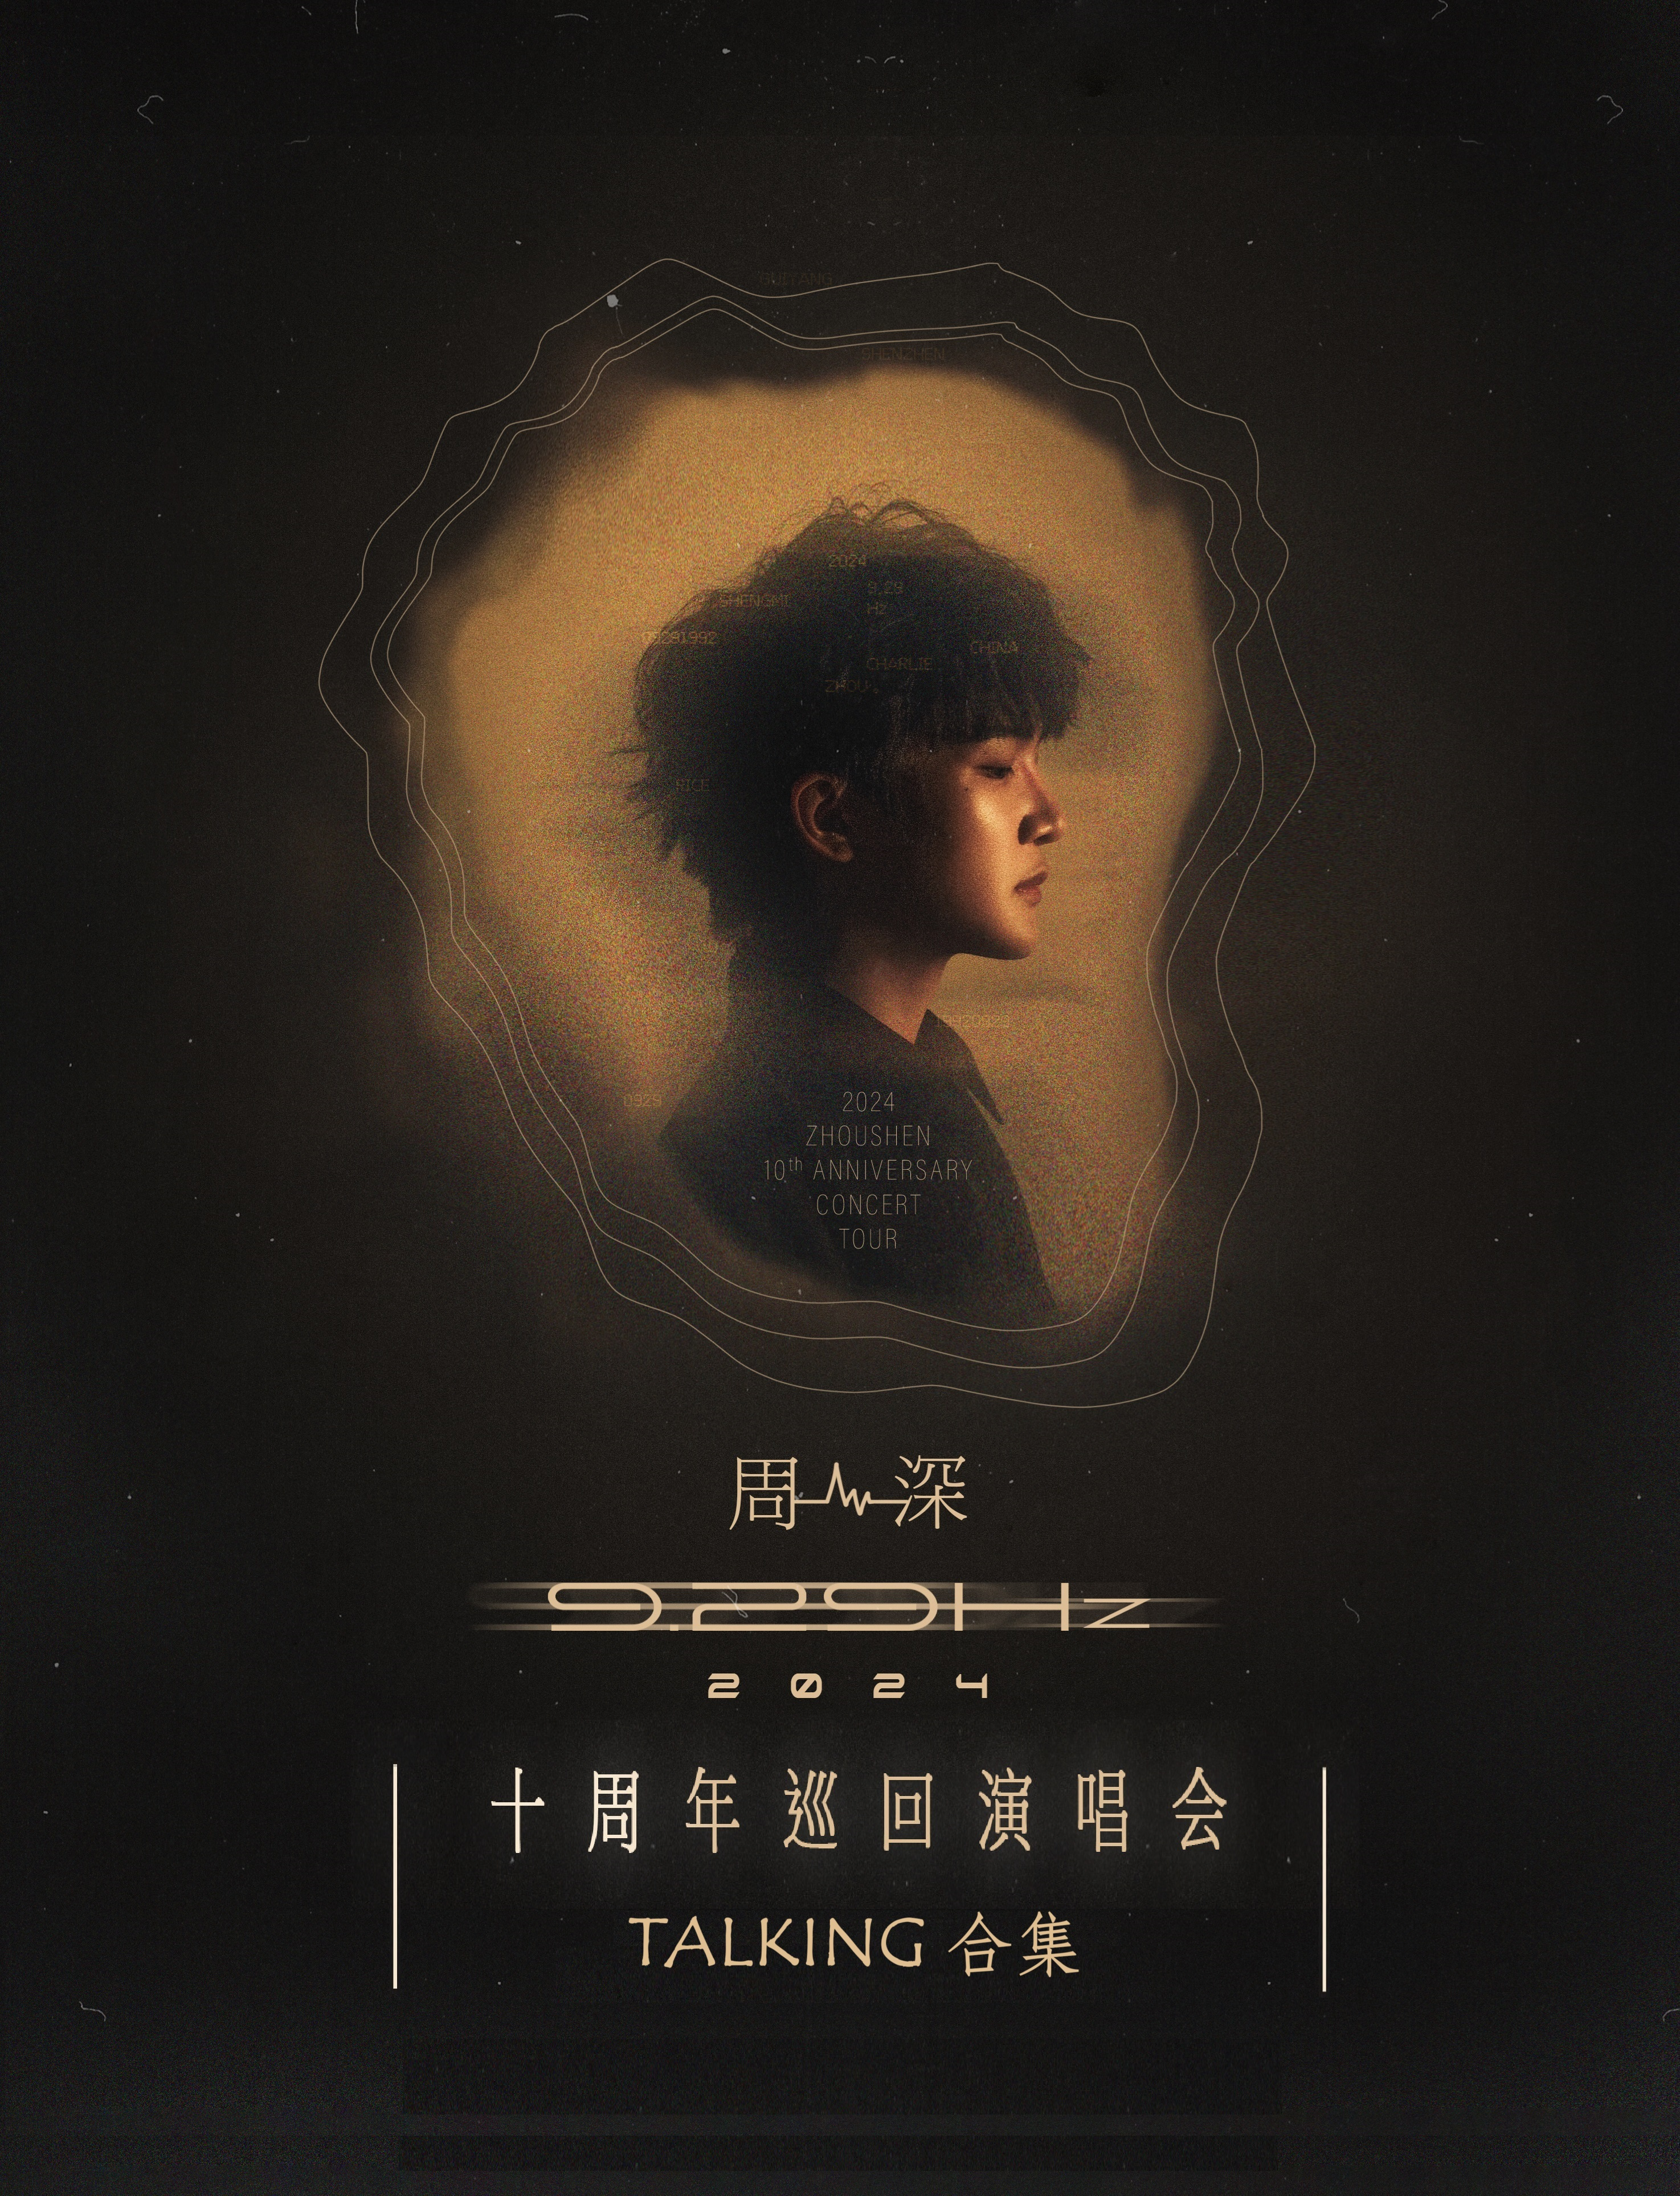
\includegraphics[width=350pt]{img/book-cover} \end{center}

\section*{关于本书}\label{about-book}


\begin{quote}
\textbf{\emph{只要你们想我的时候就可以打开那个文档。------周深}}
\end{quote}

\subsection*{1. 整理本书初衷}\label{motivation}


  在9.29Hz巡演现场,深深唱了近30首歌,同时,也讲了很多的话,其中,不仅有一些他首次透露的过往经历,也有他现场感人肺腑的情感表达,还有一些与生米的欢乐互动,而这一切的美好都值得被文字记录,在以后的岁月想起来的时候就翻开看一看,相信在这自带BGM的文字中,一定也有独属于你的美好回忆!你不必一口气读完此书,``\textbf{只要你们想我的时候就可以打开那个文档}''。

\subsection*{2. 本书结构}\label{book-structure}


  本书结构分为四部分,第一部分前言包括关于本书、推荐语、郑重声明和致谢。第二部分主体内容为每一场9.29Hz巡回演唱会深深的talking记录,每一场分为五部分,分别对应演唱会的五个部分,并附有歌单。\textbf{因为根据现场talking整理,本合集尽可能的保留原口语化说法,但部分可能有歧义的表述进行了书面化的修改,请知悉}。第三部分为巡演相关的附录,包含\hyperref[playlists]{9.29Hz巡演歌单汇总}、\hyperref[appendix-gift]{9.29Hz巡演彩带和伴手礼汇总}、\hyperref[appendix-letter]{十年来信}、\hyperref[appendix-vcr]{9.29Hz巡回演唱会VCR文字版}、\hyperref[related-929hz]{9.29Hz巡回演唱会其他相关视频、音频资源}、\hyperref[acknowledgements-list]{9.29Hz巡回演唱会致谢名单}、\hyperref[appendix-song-lyric]{9.29Hz巡回演唱会歌曲歌词}。第四部分为书中引用的相关资源原始出处,也就是学术界称为参考文献的reference。

\subsection*{3. 阅读在线版提示}\label{tips}


  本书在线版本地址为\url{https://929hz.com}。在线版可获得更好的阅读体验------对talking重要部分进行着色区分;添加链接引用,可直接跳转。如歌曲点击歌曲名字可直接跳转至附录对应歌词,每部分结束后有深深发表的微博及工作室发布的回顾视频链接;可以发表评论并支持markdown格式;支持关键字全文搜索。

\subsection*{4. 如何为本书做贡献}\label{how-to-contribute}


  本书主体部分依据现场录音转为文字,其中可能存在一些纰漏和不足之处,欢迎大家批评指正。关于本书,如果您有任何意见或建议,欢迎在页面底下评论区评论(评论需要注册\href{https://github.com/}{github}账号,可直接点击评论框下方按钮进行注册,\href{https://docs.github.com/zh/get-started/start-your-journey/creating-an-account-on-github}{如有问题,点击查看注册教程},github为最大代码托管平台,\href{https://baike.baidu.com/item/Github}{点击查看github百度百科}),也可移步小红书搜索``shenshen\_929''私信我。另外,如果你擅长画画,愿意为此书配一些图片,也欢迎联系我。

\newpage

\section*{推荐语}\label{recommendation}


  相比视频和图片,文字同样能承载关于9.29的记忆,而整理的现场talking文字合集,可以说是使用最少的容量,承载关于9.29Hz巡演最多的记忆。我能想到最浪漫的事,是多年以后,耳背的我戴着老花眼镜坐在阳光底下,翻看着这本9.29Hz巡演talking合集,记忆拉回到2024年8月11日南京场,深深唱Wala li longla时说的那句``感受这一份快乐吧,我最爱的你们!'',那一份快乐,一直陪伴着我!

------ 低碳南(我和老婆是生米)

  演唱会像是一座乌托邦,一场梦境,离开之后记忆总是逐渐被冲淡。而文字会让那时的场景又浮现在眼前,不止有声音,还有那时的心情,或快乐,或触动,那都是我们共同的经历。回忆是另一种形式的再相聚。

------ 培养基要开心

  每一次演唱,每一次相遇对我来说都是一场盛大的、自由的、绚烂的梦。在这短暂的夜晚,天籁之音萦绕在耳畔,璀璨光影拥抱缠绕着我们,灵魂放松,周遭的世界仿佛不存在,我只看到周深,听到周深。这本talking记录,让我在平凡日子里又回到了9.29Hz现场,声音和画面奔涌而来,于是,我许愿,鲜艳的人,便要这样鲜艳下去。

------ Rachel-w(策马南行英雄梦)

  9.29Hz是我第一次体验追逐巡演。从深圳场开始的听一次就好,到今年我在南昌场的第十场的十全十美收官。感谢周深给我们带来的难以言喻的美好,快乐和爱自己做自己的力量!翻看这本talking书里记录的文字,仿佛瞬间回到我参与的每一场盛会,感谢记录,让我能镌刻下这些珍贵的回忆!

------ Gillian(\_胖丁)

  这本talking合集通过文字能很直观的感受到深深从梅奔的``你们说实话,你们听完会觉得很长吗时间?''再到后来的``现在我觉得周深非常幸福。''这个小心翼翼到享受被爱的过程。这朵开在贫瘠里,长在不可能里的宝石花,开了。

------ 韩晗(pupu布长)

  时常回忆演唱会的点点滴滴,随着时间流逝看的场次多了记忆渐渐变得模糊且混乱,二专现场我都拥有了吗?点歌环节唱了什么?许许多多的细节每场三小时的视频根本盘不过来,这本书就像一份索引,能帮我快速准确地找到那个时刻。那些未能拥有的现场通过阅读talking也成了我记忆的一部分,一起构成了完整的9.29Hz十周年巡回演唱会的美好回忆。

------ 刘卷卷

  第一次听周深演唱会,虽是山顶票,却是看最美蓝海和不想睡星光的绝佳位置。有幸成为蓝海一粒摇摆像素,一切都像是梦,重温周深的语录,才能确定这不是梦,是真实存在的如梦如画记忆。

------ 姜雯箐叻

  周深的9.29Hz巡回演唱会从五月开始,13个城市,共20场。不论歌曲安排,魔术表演,舞美和talking,每一场都有不同的惊喜。众所周知,周深的talking是他按现场情况,发自內心的肺腑之言,为生米和观众送上的心灵鸡汤。周深每一现场的talking更为演出锦上添花,送观众难忘的回忆。每次奔赴后,总带着那双向的爱回家。谢谢周深。谢谢编者为大家安排,把所有talking收集成这独一无二的美好回忆。

------ 小默\_Adie

  周深的演唱会,每一场都不一样,有时,我甚至觉得,我是为了talking而来的\ldots 没有说唱得不好的意思!只是,在享受极致舞台的同时,我们也像参加了一场心灵疗愈。每次奔赴后,总能带着满满的爱、大大的力量,努力成为更好的自己。所以我常常告诉我的心理治疗师朋友,我也有我的专属治疗师,他可厉害了。他的名字叫周深。

------ 拥有三巡17场的Menie

  看着talking的文字,一会笑,一会哭,仿佛每场演唱会又重演了一遍,一幕幕画面浮现在脑海。你总说你``何德何能'',而我们又何尝不是``何其有幸''呢?能够遇见你,听见你的声音,能够与你同频,被你治愈,这都是我生命中最大的幸运!

------ 雷胖胖需要正能量(Lia\textasciitilde)

  我刚入坑时曾认为talking是演唱会的精华(现在觉得演唱会全是精华),天使在台上侃侃而谈,熠熠生辉。后来,我看了演唱会现场,太幸福的几个小时总像一场幻梦,喧闹后的寂静让我怀疑:我真的听过演唱会吗?可当我翻看这本talking书,回忆总能涌上心头,我曾经历过这样幸福美好的时光啊!于是学到颓废想放弃的我又充满力量,重整旗鼓向中考奋进。谢谢周深!

------ 看星星发光的玥啊(希望宝贝小福星能保佑我中考大捷!)

  不知不觉已经是八岁的米米啦!!!虽遗憾不能去到每一场演唱会,听到他说的每一句话,但每次翻开talking书,都仿佛把我带回那快乐的几个小时,找到继续前行的勇气!他的talking字里行间都凝聚着对生米、对歌迷的爱,能给予我学习上的动力,生活上的鼓舞。谢谢深深的每一句话,陪我度过那些挫折与困难!没有谁会不爱他!找不到答案也没关系,我一定会成为想要的自己!!!

------ 十四岁的小初生(chù shēng)小白粥里的小生米

  岁月悠悠,流光悄转,9.29Hz的那一场场视听盛宴,于记忆的长河中渐次铺展。奈何时光的风拂过,往昔亲临现场的诸般细节,竟如雾里看花,渐趋模糊、凌乱。每一曲中,仿若藏着无尽故事的神秘匣子,而这本talking仿若索引,可速且准觅得彼时诸刻。彼未临现场者,阅其文辞,亦成吾忆之一部,共构美忆之完璧也。

------ 刘子扬(叫我改改就好了)

  从春天518上海首场垂直入坑,到武汉淋过雨欢乐唱生日快乐,再到南京流过汗过七夕,从看台慢慢想往前,想离深深更近,杭州内场到苏州内场,距离一点点缩进,从像素小人到肉眼可见,南昌是我的收官场,但不是周深的!每一场talking,深深都会对我们说要好好照顾,谢谢等等话语,但其实一直想说谢谢周深,深深也要好好照顾自己,你是照耀我们的太阳,希望深深更加自信,你是最棒的!也十分感谢整理这本书的编者大大,让深深的对我们说的能够记录成册,反复回味这独一无二的回忆。

------ 米壳缝合匠

  没有人能控制住自己不去爱他!尤其是在感受到了波涛汹涌的爱意和真诚之后。别人都说每场演唱会的歌大部分都是一样的,为什么你还要去看?因为每一场都是我们期盼已久的重逢,每一句歌词都是我俩之间的温言软语。而这本talking就是我的记忆商店。爱你,宝贝!

------ always

  「爱有时不过就只求一个记得」每一次见面都想记住他唱的每一首歌、说的每一句话、每一个动作和小表情\ldots 记住三小时内哪怕一丝一毫的细节。可即便我们每一次都在用力记录,离开这场梦境后还是怅然若失。不见面的时候就打开这本talking合集吧,温存的记忆全部涌上,字字句句都告诉我们,「说完再见,还能再见」。

------ 晴空雨与鱼

  深深说,同频的人是礼物,那感谢周深让我拥有了很多很多的礼物。每一场演唱会对我来说都是一场最绚烂的梦,是生命中最浓墨重彩的那一笔,也是生活得以前进的动力和期盼。语言是情感传递的桥梁,真挚又温暖的话语总是最动人心,深深的每一句都会被接住、被懂得、被珍藏,因为我们都是彼此的礼物,谢谢周深为生米们编织的一场又一场若梦浮生,愿我们梦醒不散。

------ 七七(打哈欠的周猫猫)

  每次看完演唱会回家,都像从一场盛大的美梦中醒过来。然后开始担心随着时间流逝,那些本该深深印刻在脑海里的声音,光影,风吹过的温度,雨滴落在手上的触感,会不会逐渐变得模糊。感谢南哥整理的talking,让我可以通过这些文字来唤起一些美好的记忆,短暂的挣脱禁锢灵魂的巢,逃离到深深制造的浪漫小宇宙。

------ momo(纵然前路荆棘遍野)

  9.29hz周深演唱会的门票,我想是上天听到了我的声音,送给我的礼物!台上小小的周深总有着大大的能量,永远带给我无限的力量,也会被他的声音治愈一次又一次!小美满许愿的时候,深深给我们讲了他在深圳下雨的那个小故事,他说也许我们现在还在淋雨但也要相信爱你的那把伞一定会到!还有在重庆场限定的这是我的秋衣,冬天我离不开你,有泪又有笑。相互许愿,互相期许,生米和深深永远是双向奔赴的存在,这本talking记录着深深每一个奔向我们的瞬间,也承载着我美好的记忆碎片。

------ akira

  深深每次都说喜欢他接受他需要多一个过程,这不可否认,但这正是他的特别之处。9.29Hz我们因同频而相遇了,一场场巡演见证了深深从忐忑不安逐渐信心大增的过程,生米们一次一次证明我们的爱,深深也一次次表露出有多爱生米和歌迷朋友们!``爱要大声说出来''``完成大于完美''``我爱你们''这些都深深印在我的脑海中,希望看到本书的你们也能一起感受当时的美好心情!9.29Hz巡演即将落幕,我们的故事才刚刚开始\ldots\ldots{}

------ 田田(草莓榴莲冰淇淋)

  当灯光随着旋律变化,在舞台上勾勒出一幅幅流动的画面时,整个空间似乎都被赋予了生命。我只沉浸于一个由声音、色彩共同编织而成的奇妙世界里,忘却了外界的一切烦恼与忧愁。这份talking记录,不仅是对过往美好记忆的一种珍藏,更是对未来无限憧憬的一份寄托。它提醒着我,即使是在平凡的日子里,也可以通过回忆这些闪耀瞬间来获得力量与勇气。

------ 朱颖超(一颗简单的生米朱朱)

  这真是一篇篇自带BGM的文字,翻开耳边就响起``赫兹是每秒声音波动的次数\ldots\ldots'',仿佛置身于演唱会现场,被美妙的旋律环绕着,瞬间脱离开劳心的繁杂日常,让人沉浸其中,那份回忆就此展开\ldots 深深记得!我们永远记得!

------ 为了深深下载微博的猫猫雾

  出于对演唱会的好奇,我在人生中第一次去了贵阳。意料之外的,深深带来的,不仅是绚烂的演出盛宴,更是一场心灵的疗愈。于是,有了第二场、第三场。。。大家都说,演唱会很难戒断,当喧嚣归于平静,那就静下心看看talking吧!

------ 吃货猫\_Renee

  从最初的518梅奔场入坑到现在的逃不出去,深深的talking是我念念不忘的东西,很真诚很美好。很庆幸有纸质版东西能够记录,美美翻开,仿若回到了那些时光,或哭或笑,久久挥之不去。

------ 芸汐(戏子94看戏)

  近期参加了一个关于成长的活动,开场时需要大家写一条寄语贴在海报上,我微笑着,写下了这句:``你会成为想要的自己,找不到答案也没关系''。半年间的许多次内耗和迷茫中,这句话都给我了无限的力量。你看吧,你的话语,你写下的文字,创作的作品,时时刻刻都在影响着我们。在9.29Hz巡演的旅途中,有太多这样的治愈时刻,幸好,这些都被一一记录,整理,印刷,珍藏。深深会记得,生米更会深深记得。

------ 亮晶晶当然会发光

  9.29Hz 演唱会从春天来到了冬天,我从贵阳开始到南宁结束,我和你走过了三餐四季,一起体验了12场精彩绝伦的演出,而演出中的talking让我感动又难过,你说你不知道在舞台上还能唱多久,但是,能多唱一首是一首,你说你爱我们,你还说周深可以做到,你们也可以,可能随着时间的推移会慢慢淡忘,但是通过这本talking可以把我慢慢的带回到那时的场景中去,再次去体会其中快乐,很感谢这本书的作者南哥,让我能将这份美好的记忆珍藏!

------ 羊小杨(为你留下\_何需理由)

  我是一粒始于沈阳奥体的新米,一场高烧中的无心插柳,人生中的第一场演唱会门票竟然丝滑的进入了我的票夹。3个小时,我的心里从``咋这么客气呢''到``周深唱挺好,听众挺热情''再到``啊啊周深好真诚啊'',直到听见``证件不要掉啦,手机不要掉啦''之后垂直入坑!一晚的亢奋,第二天兴奋得回忆不出一点演唱会的细节,像一场虚幻的狂欢,终于在看到这一份talking后有了可供反复回味的载体。

------ 昵称叫萝卜的贰贰

\newpage

\section*{郑重声明}\label{declaration}


  1. 本书稿主体talking部分相关所有权归周深所有,\textbf{禁止用于商业盈利用途。}

  2. 本书稿\textbf{仅供生米交流学习使用},本人承诺不会用于任何盈利活动。

  3. \textbf{本书稿仅供免费阅读,禁止读者商用、盈利,禁止无授权转载。}

  4. 本书内容为特定语境下的口述记录,请勿外延至其他语境。

  5. 本书相关图片素材\textbf{已获作者授权}。演唱会结束周深发布的微博截图仅供学习交流,截图中转发、评论、点赞数目为截图时刻的数目,不代表当前数目。

  

\newpage

\section*{致谢}\label{Acknowledgments}


  首先,我要\textbf{感谢深深宝贝},正因为他演唱会现场说的很多非常有意义的话,才有了想要整理talking的想法。深深在演唱会上说过的话,既给我们带来了感动,也给我们带来了欢乐,不仅在现场给我们提供了情绪价值,也作为美好的回忆留存在我们的脑海里、我们的心里,深深,谢谢你!当然还有周深工作室的小伙伴们和为了演唱会付出的每一位工作人员,谢谢你们!历时数月完成本书稿,当然不止我一个人的努力,期间得到了很多人的帮助。

  \textbf{感谢``深深票哈哈娃哈哈''群里几位热情的生米给我提供的帮助。}在我未能到场观看的场次,她们提供了现场的录音,其中Gillian(\_胖丁)提供了武汉场、杭州场、南京第二场、北京第二场、苏州第二场、南昌场录音,韩晗(pupu布长)提供了上海场、深圳场录音,羊小杨(为你留下\_何需理由)提供了北京第一场、苏州第一场录音,Oli酱提供了沈阳场录音。也感谢帮我整理了部分录音的生米,其中晴空雨与鱼整理了深圳Part1,田田(草莓榴莲冰淇淋)整理了武汉场Part2、Part3部分,培养基要开心整理武汉场Part4部分、南宁第一场Part1,Rachel-w(策马南行英雄梦)整理了苏州第二场Part4渺小部分及Part5,朱颖超(一颗简单的生米朱朱)整理了南宁第一场Part3。

  \textbf{感谢为本书贡献素材的生米和老师们。}Gillian(\_胖丁)、晴空雨与鱼、韩晗(pupu布长)、雷胖胖需要正能量(Lia\textasciitilde)、羊小杨(为你留下\_何需理由)、吃货猫\_Renee、刘子扬(叫我改改就好了)等生米提供了不同场的``谢谢\_\_\_,谢谢你''图片,培养基要开心、韩晗(pupu布长)、陈叶婷(米壳缝合匠)、刘卷卷、Rachel-w(策马南行英雄梦)、芸汐(戏子94看戏)、田田(草莓榴莲冰淇淋)提供了附录B中伴手礼图片,瑾上束一提供了附录B的部分彩带米图片和彩带字条图片,LWQ提供了附录B的部分彩带字条图片。附录B灵感来源于Kimiya。书中卡通插图来源于卡布洛洛,苏州无人机图来源于昊楠不会飞。

  \textbf{感谢为本书稿矫正纠错和写推荐语的生米们}------培养基要开心、刘卷卷、七七(打哈欠的周猫猫)、深深的雾猫猫、always、芸汐(戏子94看戏)、李佩卓(wifi信号两格)、亮晶晶当然会发光、昵称叫萝卜的贰贰、momo(纵然前路荆棘遍野)、吃货猫\_Renee、Gillian(\_胖丁)、陈叶婷(米壳缝合匠)、知何似、Rachel-w(策马南行英雄梦)、朱颖超(一颗简单的生米朱朱)、韩晗(pupu布长)等。

  \textbf{感谢喜欢本书稿的生米们},你们的喜爱给了我非常大的动力!

  本书基于\href{https://bookdown.org/}{bookdown}框架进行撰写,感谢\href{https://yihui.org/}{Yihui}及相关开发人员开发了bookdown,大大提高了整理效率。感谢bookdown社区成员的相关文档,解决了我在整理本书稿在线版过程中遇到的技术问题,谢谢你们!

  最后,我想对深深说: 很遗憾未能出现在你最需要帮助和支持的昨天,但也很高兴能见证你如何一步一步走到今天,更荣幸能作为生米陪你一起走向更美好的明天。深深,在你所经历的所有不确定性中,请你确信,你的歌声、你的言语、你面对生活的态度、你与人相处的真诚、你克服困难的勇气,正影响着千千万万人,\textbf{你值得世间的一切美好!尽管大胆的向前冲吧,生米永远是你坚强的后盾!}

我和老婆是生米\\
2024.12.17

\chapter{2024.05.18上海场}\label{shanghai-20240518}

\begin{quote}
\textbf{\emph{谢谢你们愿意拥抱我每一片不完美的碎片,请相信我,我也是这样的。 ------ 周深}}
\end{quote}

\begin{figure}

{\centering 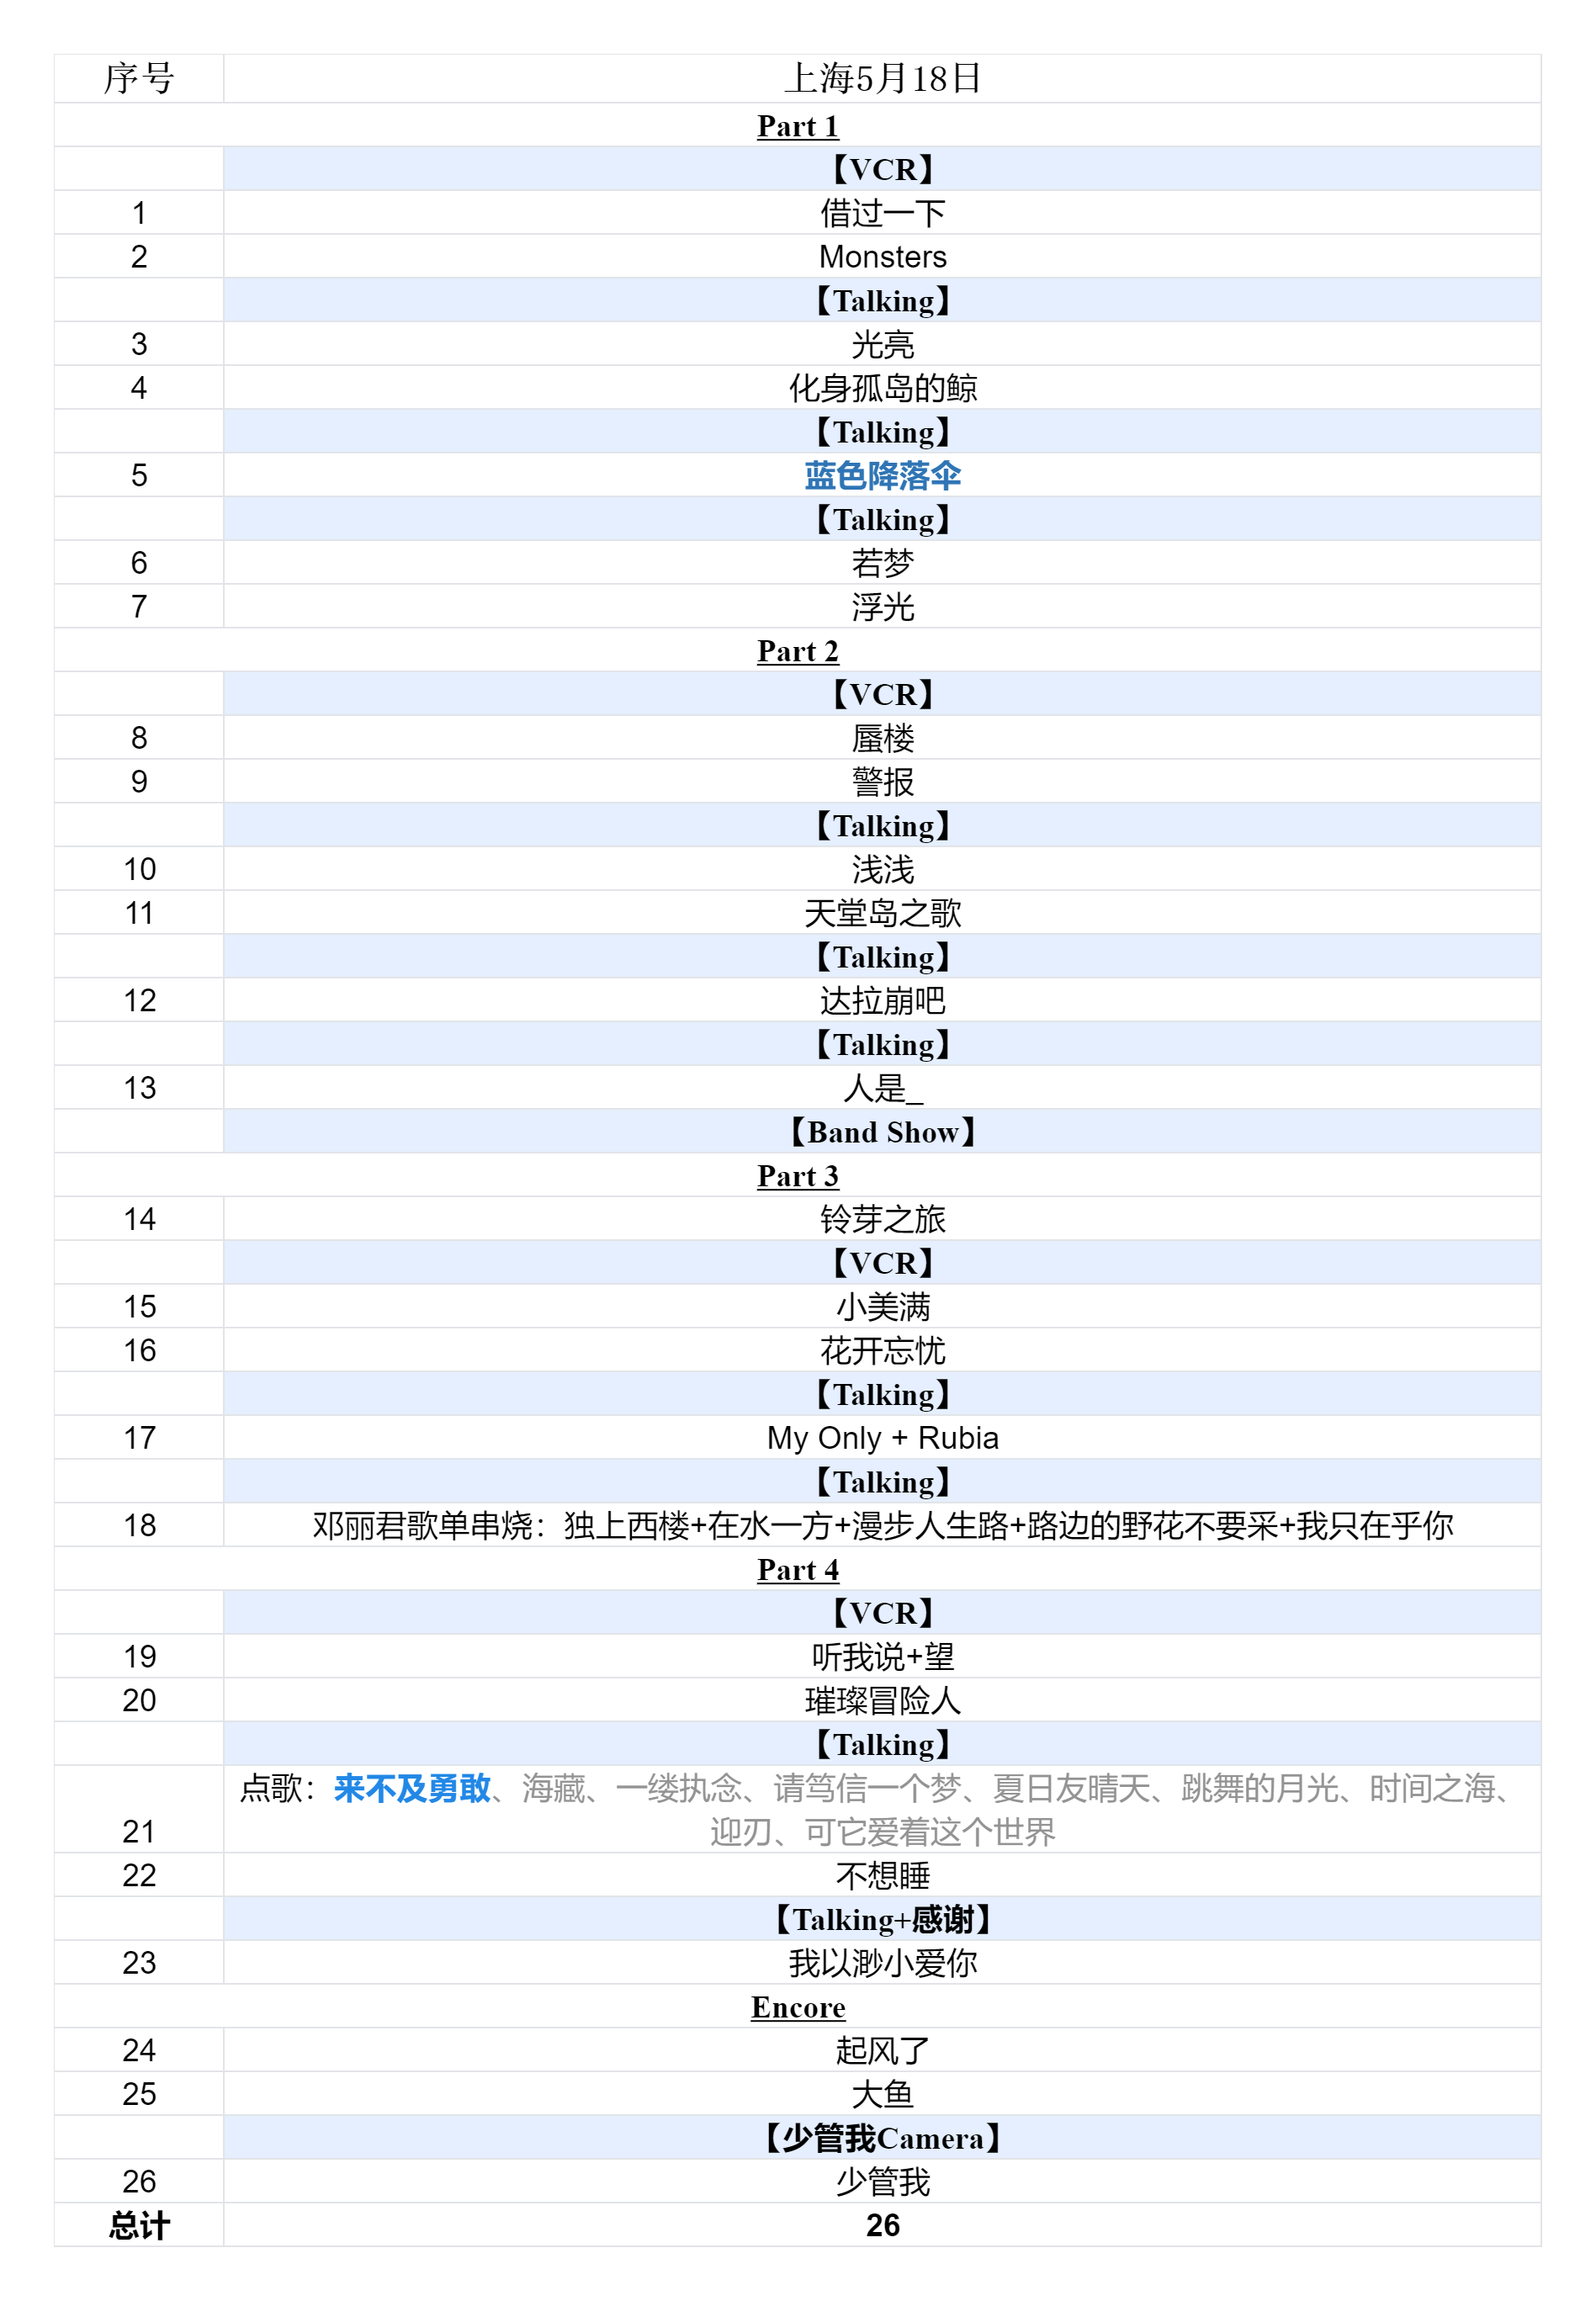
\includegraphics[width=320pt]{img/playlists/playlists-shanghai-20240518} 

}

\caption{2024周深9.29Hz巡回演唱会2024.05.18上海第一场歌单}\label{fig:unnamed-chunk-32}
\end{figure}

\newpage

\section{Part1}\label{shanghai-20240518-part1}

\hyperref[opening-vcr]{🎥【\textbf{开场VCR}】}

\hyperref[I-will-go-my-way]{🎵【\textbf{借过一下}】}你们好吗\textasciitilde{}

\hyperref[Monsters]{🎵【\textbf{Monsters}】}

  上海的朋友你们好吗?谢谢大家,9.29Hz巡回演唱会,我是歌手周深,谢谢大家,\textbf{一切真的像做梦一样},有看到很多的熟悉面孔,哈哈哈,谢谢大家,现在我们用最热烈的掌声欢迎钱雷老师,欢迎欢迎,欢迎欢迎,给大家打个招呼吧。(钱雷:hello,大家好)怎么会这么正式的打招呼?hello,大家好,你放轻松点,(钱雷:欢迎来到9.29Hz演唱会)好,谢谢雷哥,那这首歌很多人告诉我们给过他很多力量,然后也非常开心能够和雷哥一起合作,就是现场合作,这是第一次,也希望这首歌可以给你们力量,叫做光亮。

\hyperref[silver-linings]{🎵【\textbf{光亮}】}

\hyperref[hua-shen-gu-dao-de-jing]{🎵【\textbf{化身孤岛的鲸}】}你们会唱这首歌吗?(米:会\textasciitilde)到你们(米:你的衣衫破旧,而歌声却温柔)大声点(米:你与太阳挥手,也同海鸥问候)(深:我想给你能奔跑的岸头)(米:没有墙头)(深:无论你们有多少个墙头,你们都永远是王后,国王和王子)

  谢谢大家,大家好,接上我们之前的那个开场VCR,为什么叫9.29Hz,我觉得自己是一个,怎么说呢?就觉得自己应该是几乎没有可能,没有办法被大家听到的一个存在,但是却被你们听到了,所以谢谢你,谢谢。\textbf{然后你们选择用我来治愈你们,但其实你们也一直都在治愈着我}。谢谢大家,那接下来这首歌对我来说也是非常非常甜蜜,要检测一下你们听我的歌的时间有多长?这首歌叫做蓝色降落伞,有人听过吗?(米:有)明目张胆的变装时间,这样会没有惊喜,你们有听过对不对?那等下会跟我一起唱吗?(米:会)那你们要唱好听一点,你们知道为什么吗?因为制作人尹约老师今天也在,所以就是不能只是我一个人在这交答卷,你们也要交答卷,哈哈哈,我试一下啊,(深:我蓝色)(米:的降落伞)(深:在天空里)(米:那么孤单)哇你们真的会唱,那等下要跟我一起唱哦。

\hyperref[blue-parachute]{🎵【\textbf{蓝色降落伞}】}我现在很高冷,你叫我是不会理你的\textasciitilde{}\textbf{我可以高冷,但是你们不能高冷哦\textasciitilde{}}到你们(米:我蓝色的降落伞,在天空里那么孤单\textasciitilde)(深:他嘴角的那根烟)(米:忽明忽暗地走远)谢谢\textasciitilde{}

  谢谢大家,因为我看别人演唱会都是指哪里,哪里尖叫声就非常大,这是真的吗,这就真的是开演唱会就可以享受到的待遇吗?让我试一下,试一下啊,(米:啊啊啊啊)后面看台的,(米:啊啊啊啊)谢谢,谢谢,你知道为什么我要这样做?\textbf{因为我想让你们就是更开心一点,毕竟如果你们嗓子非常完美的离开这场演唱会,我会很没有面子,哈哈哈,那接下来大家合唱的时候一定要更大声一点好不好?}(米:好)但是你们已经唱得非常棒。每次我们相遇的时候都让我觉得像梦一样,真是若梦。

\hyperref[ruomeng]{🎵【\textbf{若梦}】}(米:唯愿你能得到拯救)哇塞,\textbf{唱得好哇,就该开场生米演唱会\textasciitilde{}}(米:往事流转在你眼眸)大声点,这边的\textasciitilde 看台的朋友们\textasciitilde 我们一起(深、米:往事流转在你眼眸\textasciitilde)(\textbf{深:因为你我才得到拯救})

\hyperref[floating-light]{🎵【\textbf{浮光}】}

\section{Part2}\label{shanghai-20240518-part2}

\hyperref[senself-vcr]{🎥【\textbf{反深代词VCR}】}

\hyperref[mirage]{🎵【\textbf{蜃楼}】}

\hyperref[the-giver]{🎵【\textbf{警报}】}

  刚才的歌你们觉得好听吗?(米:好听)掉装备了,\textbf{刚才的歌你们是除了业内人士的全球首听哇,我觉得是我的荣幸。}因为刚才的警报,蜃楼你们都听过了,也不一定是全部,蜃楼大部分人应该听过了,警报的话是在明天零点即将上线的专辑反深代词里的歌曲,作曲钱雷老师,作词尹约老师,我觉得自己都非常幸福,可以有这么多老师愿意去帮助我,让我被大家听见和看见,谢谢这些老师们,谢谢谢谢。那接下来这首歌莫名的会觉得跟前面两首歌气氛很搭,我叫周深,以前我最受不了的名字就叫,深\textasciitilde 但是没想到慢慢慢慢的习惯了别人叫我深深\textasciitilde 那这首歌刚好也很反深代词,因为他叫浅浅。

\hyperref[qianqian]{🎵【\textbf{浅浅}】}

\hyperref[haven-song]{🎵【\textbf{天堂岛之歌}】}

  谢谢大家,大家好,再自我介绍一下,我是歌手(米:周深),谢谢谢谢。为什么这里要打断一下?因为害怕有人听完回去不敢睡觉,哈哈哈,会吗?(米:不会)我只听到不会的声音,但是肯定也会有吧。总之,就是下面这首歌,算是一个老考题了吧,我形容一下,它是一个很热闹的歌曲。(米:达拉崩吧)这么快就猜中,我岂不是很没有面子,我再给一个稍微明显一点的线索,他的名字好难念,(米:达拉崩吧)什么(假装听不见)?你们还没有猜出来,你们,你们真的有听过我的歌吗?那这首歌叫做(米:达拉崩吧),你们会跟我一起吗?(米:会)

\hyperref[dalabengba]{🎵【\textbf{达拉崩吧}】}不愧是国王,一听就记住了\textasciitilde 现在到你们跟我说这个故事喽,你们准备好了吗?(米:准备好了)于是\textasciitilde 后面的朋友,加快\textasciitilde{}

  最后,公主和王子过上了幸福的生活,故事到这里就结束了,哈哈。那接下来我们再一次掌声请出钱雷老师,现在你得给大家多说一下话,诶,我的生米或者是布丁对钱雷老师肯定很熟,你如果要介绍自己的话,你一般怎么介绍自己呃?(钱雷:呃,我是深深最好的朋友)可是别人会说深深是谁,哈哈哈,我觉得介绍一下,像雷哥,介绍他最简单就是用他的作品,我觉得大家都会唱,爱你(米:孤身走暗巷),还有(深:祝你踏过)(米:千重浪能留在爱人的身旁),没事唱多一点,他应该不会收我的钱,是吧?你会收吗?(钱雷:我发现我给别人写的歌你都挺喜欢)哦,是吗?(深:而我将爱)(米:你所爱的人间,愿你所愿的笑颜)嗯,还有跟我们尹约老师,我特别喜欢的一首,(深:我被爱判处)(米:终身孤寂)好,不要再唱了,再唱下去我的面子往哪搁呀?哈哈哈,你刚在那站着尴尬吗?(钱雷:还好)还好,那这个场子交给你来掌控。大家掌声鼓励他,原来欺负i人是这种感觉。(钱雷:我错了,哈哈哈,我错了)

  接下来要演唱的这首歌,我经常都会问``雷哥你是人吗''?居然写这首歌,``你是人吗?''因为这首歌的名字叫做(米:人是\_)。

\hyperref[renshi]{🎵【\textbf{人是\_}】} 掌声给雷哥\textasciitilde{}

\section{Part3}\label{shanghai-20240518-part3}

\hyperref[travel-lingya]{🎵【\textbf{铃芽之旅}】}大家好,你们还听得开心嘛?(米:开心)好的!谢谢你们\textasciitilde{}

\hyperref[close-door-vcr]{🎥【\textbf{关闭客服大门VCR}】}

\hyperref[happy-ending]{🎵【\textbf{小美满}】}大家好,愿意跟我一起唱这首歌吗?(米:愿意)大家一起哦\textasciitilde 后面的\textasciitilde{}\textbf{哇,你们唱的太好了,这绝对是我超级大的美满,谢谢你们\textasciitilde{}}怎么还改词啊你们\textasciitilde 大声\textasciitilde 谢谢你们,其实遇到你们是真的是我发自内心最大的美满,而且有人一直告诉我这首歌听完就会觉得很幸福,你们听这首歌的时候觉得幸福吗?(米:幸福),当我听这首歌的时候,我觉得所有的愿望都会实现,因为我遇到了你们,积攒着这一些小美满从一个普通的男孩慢慢站到了自己梦想的舞台,所以我觉得我们不如在这首歌一起许愿吧。我先做一个示范,321,哇,这样我们的愿望就能挂上去,所以你们愿意陪我一起许个愿望吗?(米:愿意)那大家要听话,因为现在你们无论是年纪大小,你们都是最可爱的小朋友,闭眼睛,看哪个小朋友还没闭眼睛,闭眼睛,默默心中许一个愿望,但是这里会有一个要求,这个愿望必须关于自己,要像小美满这首歌一样,无论任何时候都要好好爱自己,也一定会有很多很多人爱我们,但是我们要爱自己,许好了吗?我喊321睁眼哦,321\textasciitilde 谢谢你们,谢谢你们听得见我的愿望,你们的愿望我也都听得见,我们一起向前好吗?(米:好)

\hyperref[no-worries]{🎵【\textbf{花开忘忧}】}(深:若记忆被偷走了,忘了我的爱,我会说)(米:你好啊)你好啊\textasciitilde{}

  你们也一定要好好照顾好自己哦,(米:好)谢谢。诶,我们这里有没有之前去过北京场的深深感谢你(米:有),有这么多,那岂不是查重率百分之?在北京那一场的时候大家记得花开忘忧我在(米:弹琴),然后我碎了一地。哈哈哈,这一场,我又要弹琴,(米:哇)我是不太明白你们在哇什么,要说弹琴,明明有我们弹得非常好的键盘老师,也有雷哥,所以我弹琴你们在哇什么?\textbf{但是我觉得这两首歌非常的幸福,所以我觉得我想弹给你们听。希望我们好好爱好自己之后,我们一定可以去享受这个世界的所有,谢谢你们。}

  哇,这个舞台超漂亮的有没有?这个舞台远处看起来是一棵树,树呢,是生命,然后中间有看到跟科技的结合。所以每个人座位上都会有一个小种子,大家可以回去种一下,我觉得说不定可以开出非常漂亮的花,但是如果你担心自己养不活它的话,不用害怕,这个事情在我身上发生过很多次,大不了再种一颗嘛。好了,我要开始唱歌了,我要开始弹琴,我要开始边弹琴边唱歌,救命啊我要碎了。但这首歌我觉得送给大家非常好,(米:啊啊啊)只是一个和弦而已,朋友们,哈哈哈,重来一下,啊啊啊好紧张啊,来喽\textasciitilde{}

\hyperref[my-only]{🎵【\textbf{My Only}】}

\begin{figure}

{\centering 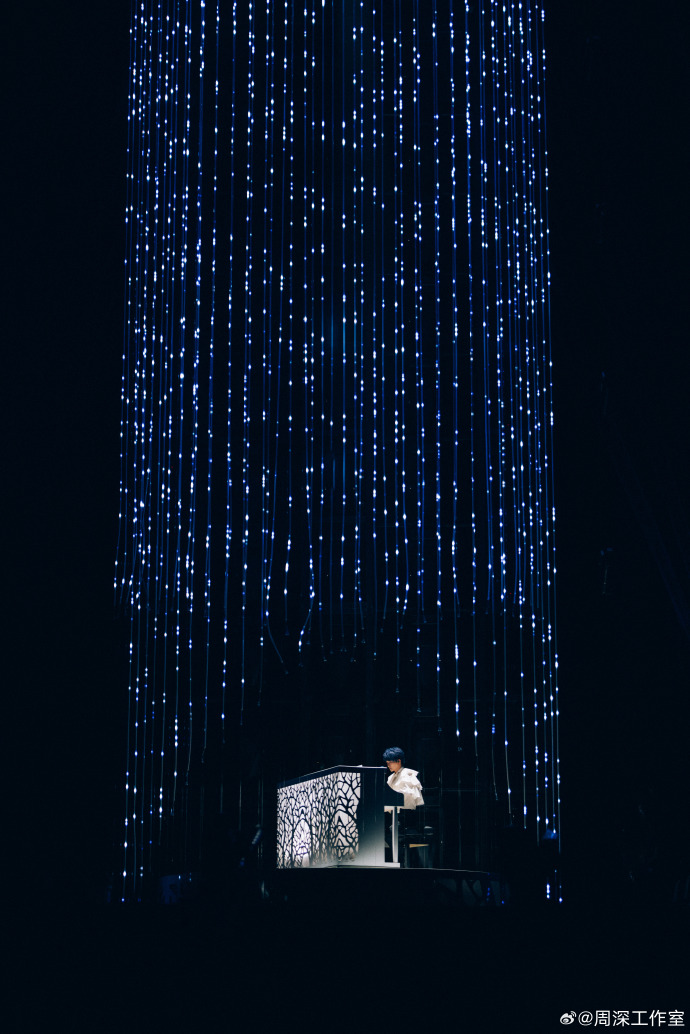
\includegraphics[width=400pt]{img/shanghai20240518/001} 

}

\caption{上海518弹琴}\label{fig:unnamed-chunk-33}
\end{figure}

\begin{figure}

{\centering 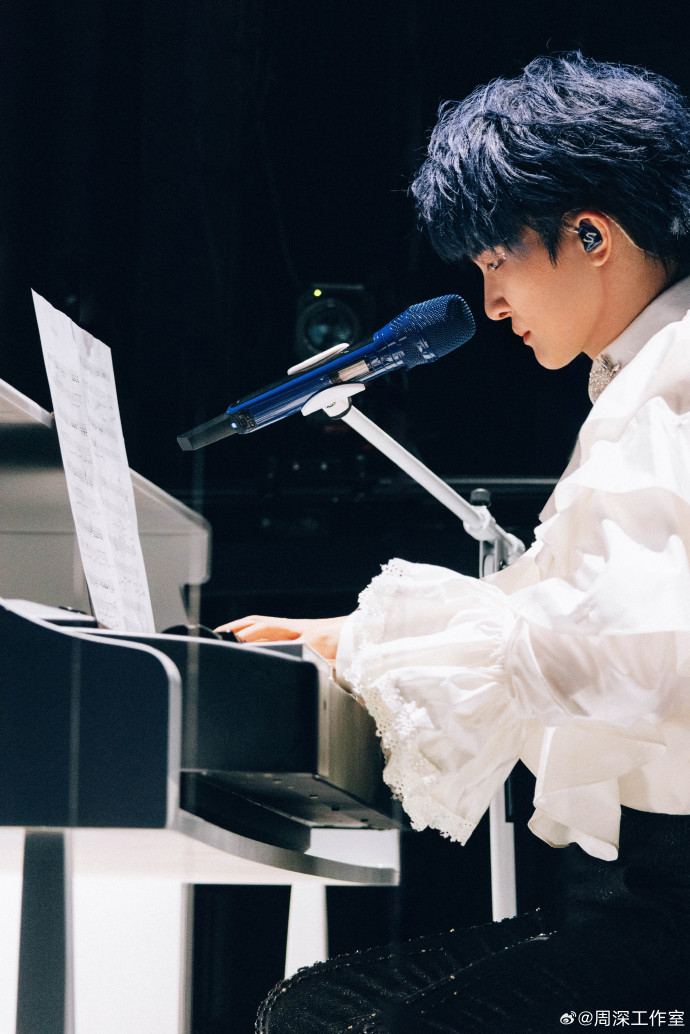
\includegraphics[width=400pt]{img/shanghai20240518/002} 

}

\caption{上海518弹琴}\label{fig:unnamed-chunk-34}
\end{figure}

\hyperref[rubia]{🎵【\textbf{Rubia}】}谢谢你们愿意拥抱我每一片不完美的碎片,请相信我,我也是这样的。

  \textbf{哇,说实话中间有一段都快忍不住眼泪,因为我有看到很多很多非常熟悉的面孔,有布丁,然后有在深空间的时候就听我唱歌,那也有在929星球的时候听我唱歌,但是无论你们任何时候出现在我生命当中,都是非常闪亮。}老师你怼到我的上嘴唇了(换衣服)。如果熟悉我的朋友的话都会知道,(我)想在自己的演唱会当中加一个致敬环节。这个环节是(米:邓丽君)oh,那熟悉我的人真的还挺多的,是邓丽君女士的串烧,我觉得希望自己可以像她一样,有很多的歌,过了很多很多年,还会被人听,还会被人唱,我也希望用这一些串烧去想起每一个朋友的回忆吧,来喽。(米欢呼)你说什么我听不见。

🎵【\textbf{邓丽君组曲}】
\hyperref[one-in-the-building]{🎵【\textbf{独上西楼}】}来来来,29号桌的朋友点了一首什么歌?听不到啦
\hyperref[on-the-water-side]{🎵【\textbf{在水一方}】}
\hyperref[walk-the-road-of-life]{🎵【\textbf{漫步人生路}】}摇起来\textasciitilde 这边的朋友,你们要听什么歌?我听不到哦,再大声点,你喊破喉咙我也是听不见的\textasciitilde{}
\hyperref[only-with-me]{🎵【\textbf{路边的野花不要采}】}所有人的墙头,都得藏好了(深:路边的野花,你不要采\textasciitilde)(深:千万不要把我来忘怀)你们会忘记我吗?(米:不会)
\hyperref[only-you]{🎵【\textbf{我只在乎你}】}(深:除了你)(米:我不能感到一丝丝情意)(深:情意\textasciitilde)谢谢大家\textasciitilde{}

\newpage

\section{Part4}\label{shanghai-20240518-part4}

\hyperref[thank-you-vcr]{🎥【\textbf{谢谢上海,谢谢你VCR}】}

\begin{figure}

{\centering 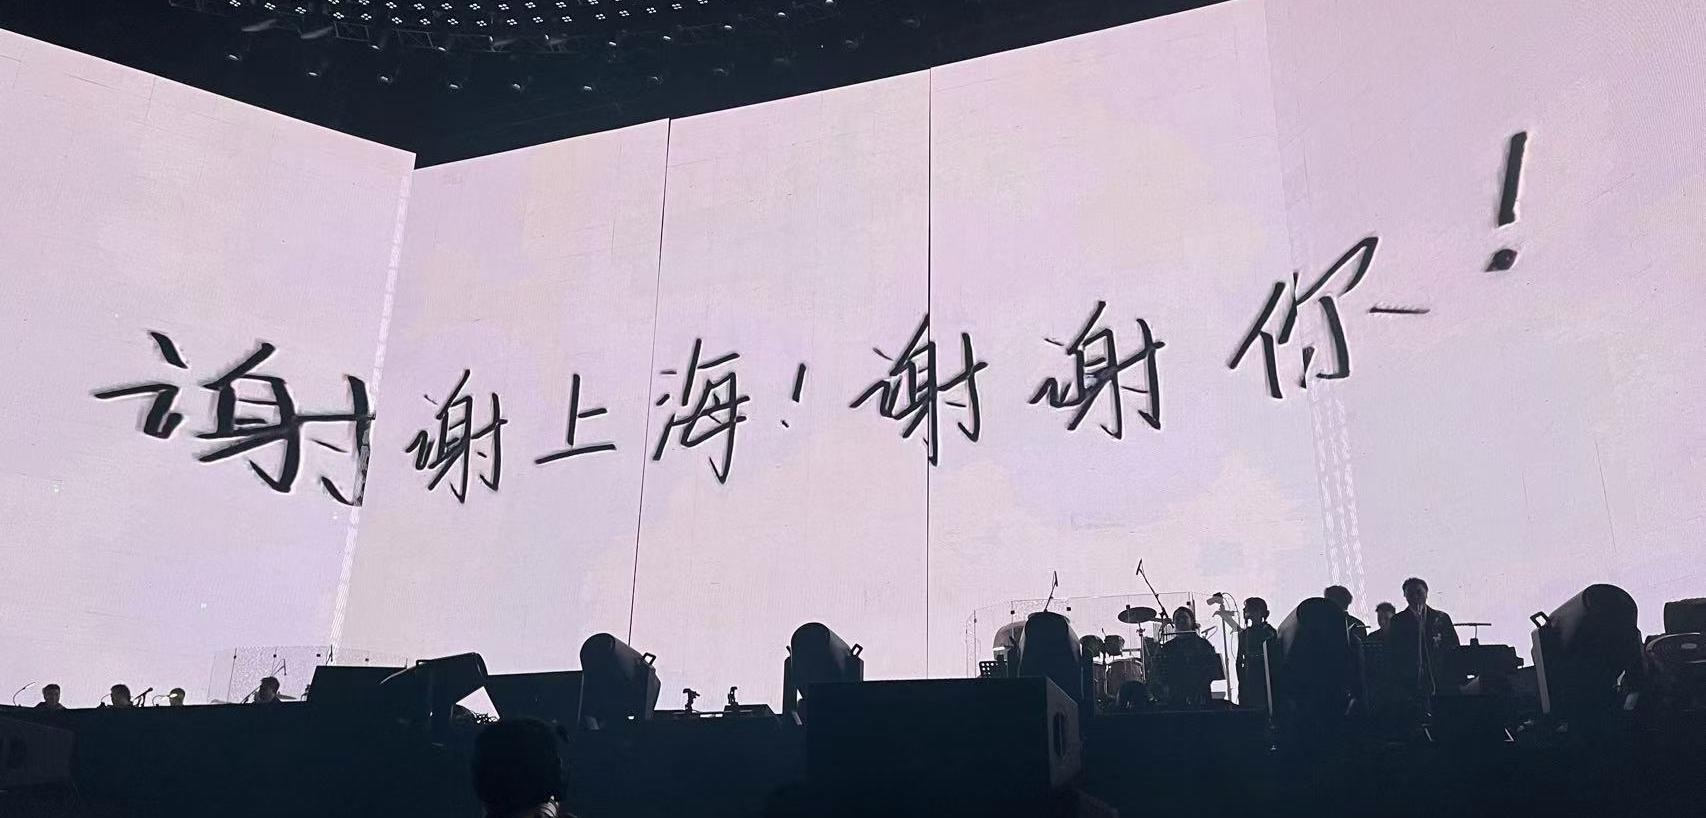
\includegraphics[width=400pt]{img/shanghai20240518/thank-shanghai} 

}

\caption{谢谢上海!谢谢你!}\label{fig:unnamed-chunk-35}
\end{figure}

\hyperref[listen-to-me]{🎵【\textbf{听我说}】} 一起(深、米:听我说,可以听我说\textasciitilde)\textbf{我也一定懂你们想说的话的\textasciitilde{}}

\hyperref[hope]{🎵【\textbf{望}】}(深:我们总会)(米:绕啊绕,绕啊绕\textasciitilde)因为你,(深:我心有所住)

\hyperref[adventurers]{🎵【\textbf{璀璨冒险人}】}你们也都是英雄\textasciitilde{}

  最大的掌声给我们的舞蹈老师们,\textbf{好帅好帅好美好美好棒好棒好会跳}。平时我也会,我自己也是个歌迷嘛,在成为歌手之前,然后最近有看到很多人都在开演唱会,哇,真的好羡慕,哈哈哈,然后他们都会有点歌环节,那我就觉得,啊,别人家孩子有的,我们家也要有。但是,可能会有一点点不一样,就是我觉得我害怕大家坐在下面会太无聊,你们坐下面会无聊吗?(米:不会)所以我会把大家比较熟悉的歌就几乎铺满,让大家更可以就是尽情享受一点点。然后这个点歌环节呢,我们已经把歌名打在了屏幕上,目前是只有9首,所以是在9首当中任意选一首都可以唱,有你们要听的吗?(米:有)真的有还是假的有,说真的有的说一句?假的有的说一句,假的有的出去一下,哈哈哈,看看那里绿色亮灯那个安全出口。

【\textbf{点歌环节}】好,那现在我们的摄像老师,会随机抓取一个朋友,让摄像老师给我们看一下你的热情,你的疯狂。随着我们全场喊321,摄像老师就会随机的zoom· in到一个朋友,你就可以点歌了,同时也恭喜你获得了``得罪''整场的这个权利。但是,我觉得也是个开心的事情,对不对?好了,我们开始摇晃起来,我们一起喊321哦,那老师你可以摇得更快一点,来喽,54(米:321)好,就是这位朋友,hello,你放心,你没有麦克,因为麦克只有我有,对不起,认清一下这是谁的演唱会,你怎么可能会有麦克?哈哈哈,大声喊出,我们应该怎么称呼你?你就在这啊?哈哈哈哈哈哈,我以为是在看台或者在后面,结果就在我第二排,看里面,哈哈哈。怎么称呼你?怎么称呼你?啊第一排,好了好了,还委屈你说成第二排是不是?哈哈哈,怎么称呼你?小斗?小朵?小朵?名字好多啊老师,这上面,诶,你从哪里来?上海?哦,你是上海这里的,(深:上海话)等一下,我最后三个字怎么那么像在骂人,哈哈哈。好,下面有你想听的歌吗?你大概从什么时候开始听我的歌的?2020年,你坐在第一排就是,你不用麦克我都听得见你在说什么。好,先点一首歌吧,哪一首歌你是最喜欢的?都喜欢?都喜欢的话我们就会觉得这应该是弃权,你们以为你们治得了我?朋友们,搞清楚好不了,谁的演唱会啊?你要听几号歌?2号?2号什么歌?2号,来不及勇敢,那看来你听我的歌真的听的有一段时间,谢谢你的支持,谢谢,小小什么来着?小斗?小朵?小斗?你叫什么名字?安静一下,你大声喊321,董小姐,怎么这里还有埋梗的,哈哈哈,好的好的,小董,原来你叫小董啊?我刚喊了她这么多名字,没有一句是叫对的,\textbf{哪怕我有个葫芦我也收不进来,大声喊你的名字,你敢答应吗?}那我们现在就准备唱这首,来不及勇敢。献给我们每一位朋友哦,我们还得说一句的是,就是点完,点完之后的歌它就会消失在歌单上面,到了下一场就可能会替补为另外的歌曲。所以只有我们上海的朋友能听到这首来不及勇敢,谢谢大家,小什么?小董。

\hyperref[late-to-be-brave]{🎵【\textbf{来不及勇敢}】}那你们会唱吗?(米:会)怎么可能\textasciitilde 然后会唱的跟我一起唱好吗,唱大声一点,尤其是小董朋友,大声一点的唱\textasciitilde 到你们(米:都是我还来不及学会勇敢,让你一个人走散\textasciitilde)谢谢大家\textasciitilde{}

  真的很感慨,这是一首非常非常久的一首歌,然后刚才也看到了,应该就是我刚出道的时候,就带我去认识这一行,去教我如何做歌手的老师们,我觉得自己很幸福,可以一路上遇到这些老师们。然后大家觉得今天听的声音好听吗?(米:好听)好,非常感谢金少刚老师,大家叫他师傅,叫他少爷。就很多时候,就我的性格大家都知道,不太会去打扰别人,但当你自己需要帮助的时候,老师们都会愿意出来帮你一把,你会觉得,哇,这世界真温暖。\textbf{所以我每次一回头,我一看见布丁,我的生米,然后听过我歌的歌迷,你们都愿意来看我,也是我莫大的荣幸,非常感谢大家,再一次感谢大家。}

\hyperref[keep-playing]{🎵【\textbf{不想睡}】}摇起你的荧光棒好不好?看台的朋友让我看到你们哦,后面的朋友你们好吗\textasciitilde 谢谢大家\textasciitilde{}

  太感慨了,谢谢你们,就很多时候,有一种是想说的话太多,你突然不知道从何说起。\textbf{刚才唱那首歌的时候,脑海中不断的会有很多的画面},从以前卡布的时候,大家都会觉得,哇你唱歌很好听,从那个评论那个留言数,0123,1千、1万、10万,或者是更多更多的数目,你会觉得自己何德何能?我会不停地告诉自己,周深你是非常非常非常幸福,而且\textbf{今天站在梅奔会对我来说意义非常重大。}我觉得这是我自己跟我的歌迷朋友我们一起设定的一个小目标,我觉得每个目标能够到达的时候一定要去看一下,看完之后算是在某个阶段给自己一个交代,才可以继续更好的往前走,所以真的非常感谢到来的每一个你,谢谢你听到我的声音,谢谢你。

  当然我们也要非常感谢所有支持我们,让我们更好相遇的背后的朋友们,让我们感谢场地支持梅赛德斯奔驰文化中心,我们也要非常非常感谢上海市公安局治安总队,让我们好好的见面,上海市公安局浦东分局、上海市文化和旅游局。感谢上海市文化市场行政执法总队。热情一点,再来,感谢浦东新区文化体育和旅游局,感谢上海市消防救援总队,感谢浦东新区消防救援支队,以及其他所有部门的大力支持,让我们能安全平平安安、开开心心的见面,谢谢他们。然后也要非常非常感谢本次巡演的全程主办,北京时代立方文化传播有限公司。我为什么这里要停顿,你们对这个名字熟悉吗?有熟悉的人都会知道,应该是从我自己第一个比较有点规模或者有点模样的巡演开始,就一直是在跟我们北京时代立方一起合作。就那个时候我就觉得,哇,你是怎么从那么多人当中看到我?就像你们从那么多人当中听到我一样,我觉得就每次,(米:你优秀)谢谢,谢谢,我不够优秀我不够优秀,我还可以更优秀,我再继续加油,但是就像刚才那个弹钢琴的片段一样,我觉得你们愿意去接受我每一个哪怕他所谓不完美的碎片,我都觉得非常非常安全,安全得非常非常舒服。谢谢你们,谢谢,感谢上海站协办TME Live腾讯娱乐超现场,感谢我们的演唱会制作单位必应,感谢我们的总导演周佑洋,感谢庄惟惞,以及让我们大家听得这么享受的音乐总监金少刚。哈哈,说错了,音响总监金少刚,感谢我们的音乐总监龙隆老师,以及用最热烈的掌声感谢我们的乐队老师们,和声老师们,以及我们的舞蹈老师们,也非常非常感谢我们的钱雷老师,大声点,要不然他(在后台)听不到,123,看来我真的很害怕你的嗓子完好的出去。好,还要感谢我们的舞蹈团队SDT ShowPro,感谢我们的服装团队设计师劳伦斯许工作室,以及时装品牌Windowsen,sensen。感谢音响工程南京奥斯泰视听科技有限公司以及我们的调音团队乐尔工作室、硬体工程北京力超舞台集团。以及感谢周深工作室的小伙伴们,(米:啊啊啊啊啊啊啊啊)偏心了吧你们?哈哈哈,感谢票务总代理大麦网,感谢票务代理猫眼票星球,感谢微博,感谢微博音乐、感谢微博演出,以及感谢我们所有现场的工作人员们,谢谢大家。当然,更重要的是感谢每一个和我们见面的你\textasciitilde 感谢我的生米,感谢布丁,感谢歌迷,谢谢大家。

  那我们来合张照吧,大家安安全全的,平平安安全坐着,来,中间,中间3,哎呦,321,好,左边,这边哦,123,呜呼,左边的,我是穿着白裤子在这里摸爬滚打,起来就变成黑裤子,321。

  好,谢谢大家,刚才,如果熟悉我的朋友的话,知道不想睡是属于卡布的晚安曲,也就是说演唱会要到尾声了,你们跟我说实话,你们听完会觉得很长的时间吗?(米:不会)那很开心的是周深也有一首比较适合他的晚安曲,我以渺小(米:爱你)。

\hyperref[loving-you-in-my-humble-way]{🎵【\textbf{我以渺小爱你}】}谢谢你们,哪怕我的力量不够大,你们还是愿意支持我\textasciitilde{}

\section{Part5}\label{shanghai-20240518-part5}

\hyperref[the-wind-rises]{🎵【\textbf{起风了}】}谢谢你们\textasciitilde{}

\hyperref[big-fish]{🎵【\textbf{大鱼}】}

  刚刚倒流回最初的相遇我差点笑出来,是最难的相遇吧,哈哈哈,相xu\textasciitilde 倒流回最初的相xu\textasciitilde,再来一遍,(深:倒流回最初的)(米:相遇)谢谢,哪怕任何一次的相遇,再困难我都知道我们一定会相遇,谢谢你们。好了,那其他时候我们看音乐节,怎么到处,感觉我随时都在玩的感觉,看音乐节或者演唱会别人会有一些kiss camera,就是拍到谁的话就要亲,然后或者是那个拥抱,拍到谁谁就要拥抱。(米:咦\textasciitilde)我们没有,放心,你看我了不了解你们,哈哈哈,我一说到 kiss camera,所有都是啊,哈哈哈,但是在我们这里有一个新的camera,新的一个环节叫少管我,我们先一起大喊一句123嘿,(米:少管我),\textbf{好凶的一群人,哈哈哈},大家呢要学一下手势。就是,嘿,少管我这四个字时候要,嘿,少管我,好不好?我们来试一下,试一下朋友们,朋友们,给点面子,给点面子,来123,嘿,不要打到前面的头,哈哈哈,你直接给别人来当头一棒槌,哈哈哈,好了,小心注意安全,321,嘿(米:少管我),不够有态度,再来321,(米:嘿,少管我)。没错这个才是我要的效果,就是感觉我们随时都可以把生活当中的不开心全部都喊开,那些不开心都少管我。

  所以当我们这个摄像机他照顾到谁的时候,你要凭借着没有麦克风的情况下让你喊出来的少管我,配着那个姿势响彻梅奔,你做得到吗?试一下了啊,来了哦,我们还是一起喊321,来,我们摄像老师开始滚动,321,好,看我们找到的是谁?好,就是你,先告诉我你在哪里?好,又在这里,好,老师,下一个可以摇远一点。哈哈哈,我们应该怎么称呼你?小潘?\textbf{大家都是一家人,都姓小就对了。}哈哈哈,小潘你好,你是来自哪里的?你是无锡的,在南京上学,来到了上海听我的演唱会,包邮区啊你,很开心很开心,你从什么时候开始听我唱歌?19年?有些年头了,现在已经是我出道第十年了。那你可以,你觉得你有这个信心,让我们最远的看台的朋友们听到你喊的少管我吗?你有,我甚至都没有听到你说的你有,哈哈哈哈,大家安静,给他一点面子来,你有吗?有,但是不多,哈哈哈,好了,那个姿势,那准备好了,把我们所有的不开心全部都喊开好不好?所有的烦恼全部都喊开,他们都会离你而已,声音越大离得越远。好,来,321,老师帮我,谢谢你,谢谢小潘。

  老师,现在来迅速帮我找一个我们后排一点点的,32(米:1),立马zoom in,zoom in,就是他,你在哪里?你在,哈哈哈,我们的朋友,呃是这个吗?怎么称呼你啊?哦,完全听不到。哈哈哈,我现在感受到了后面的朋友听我们小潘的声音,应该怎么称呼他?旁边朋友告诉我一下,小张?小丽?小什么?小美满?小什么?等一下我读一下你的唇语,等一下,小张,诶,小张,好,来喊出来。321,没有听到,哈哈哈,但是谢谢小张。好,那大家现在跟我一起哦,123,嘿,(米:少管我)呀呼\textasciitilde{}

\hyperref[watch-ur-manners]{🎵【\textbf{少管我}】}大家好\textasciitilde 一起来哦\textasciitilde 来喽,嘿(米:少管我),等下你们要喊大声一点好不好,我们再来一次哦,让我听到,54321,(米:嘿,少管我)好凶的一群人啊,但是我们最棒的哦\textasciitilde 大家一起\textasciitilde 来喽,大声点\textasciitilde{}\textbf{希望给你们个快乐的回忆},好不好?(米:好)我们再来一次全场所有的不开心喊出去,54321(米:嘿,少管我)这边的朋友喊大声一点哦,54321,(米:嘿,少管我)你们是最棒的,全场123,(米:嘿,少管我)谢谢大家,大家的东西不要掉了,回去注意安全,手机、身份证,所有东西都不能掉了。右边的朋友321,呦吼,中间的朋友321,走,看台的朋友321,hi,谢谢你们,我们下次见,注意安全,谢谢你们,好好照顾好自己,谢谢你们,拜拜!

\begin{figure}

{\centering 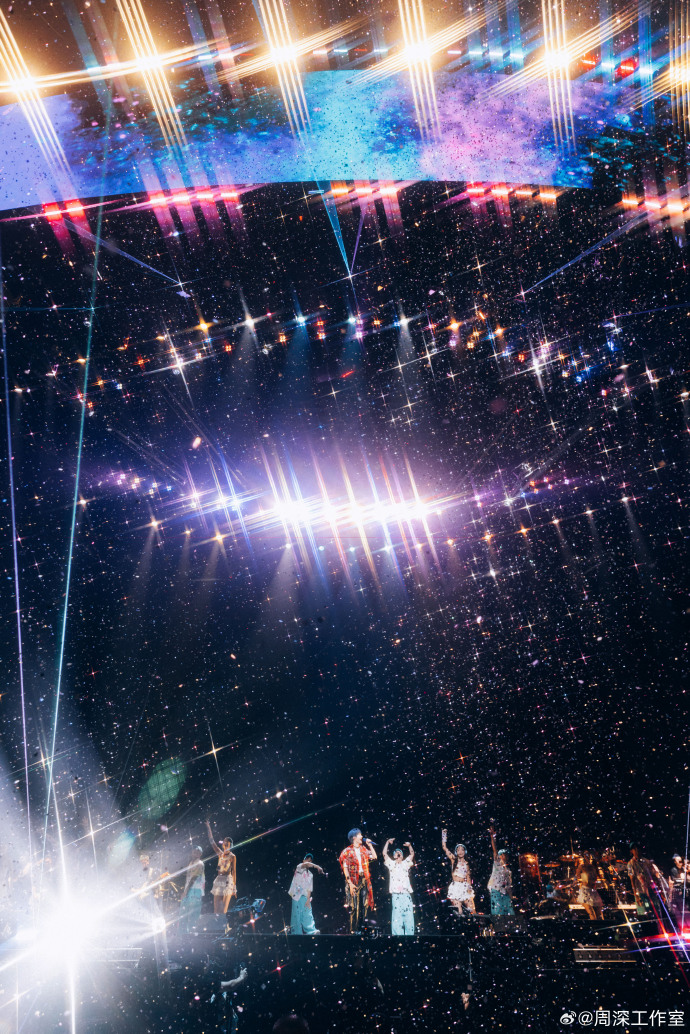
\includegraphics[width=360pt]{img/shanghai20240518/003} 

}

\caption{用这段旅途来结束今日的束缚 【@weibo-charlie-studio】}\label{fig:unnamed-chunk-36}
\end{figure}

\chapter{2024.05.19上海场}\label{shanghai-20240519}

\begin{quote}
\textbf{\emph{谢谢你们给我的快乐,我也希望能够给你们所有的快乐,谢谢你们。 ------ 周深}}
\end{quote}

\begin{figure}

{\centering 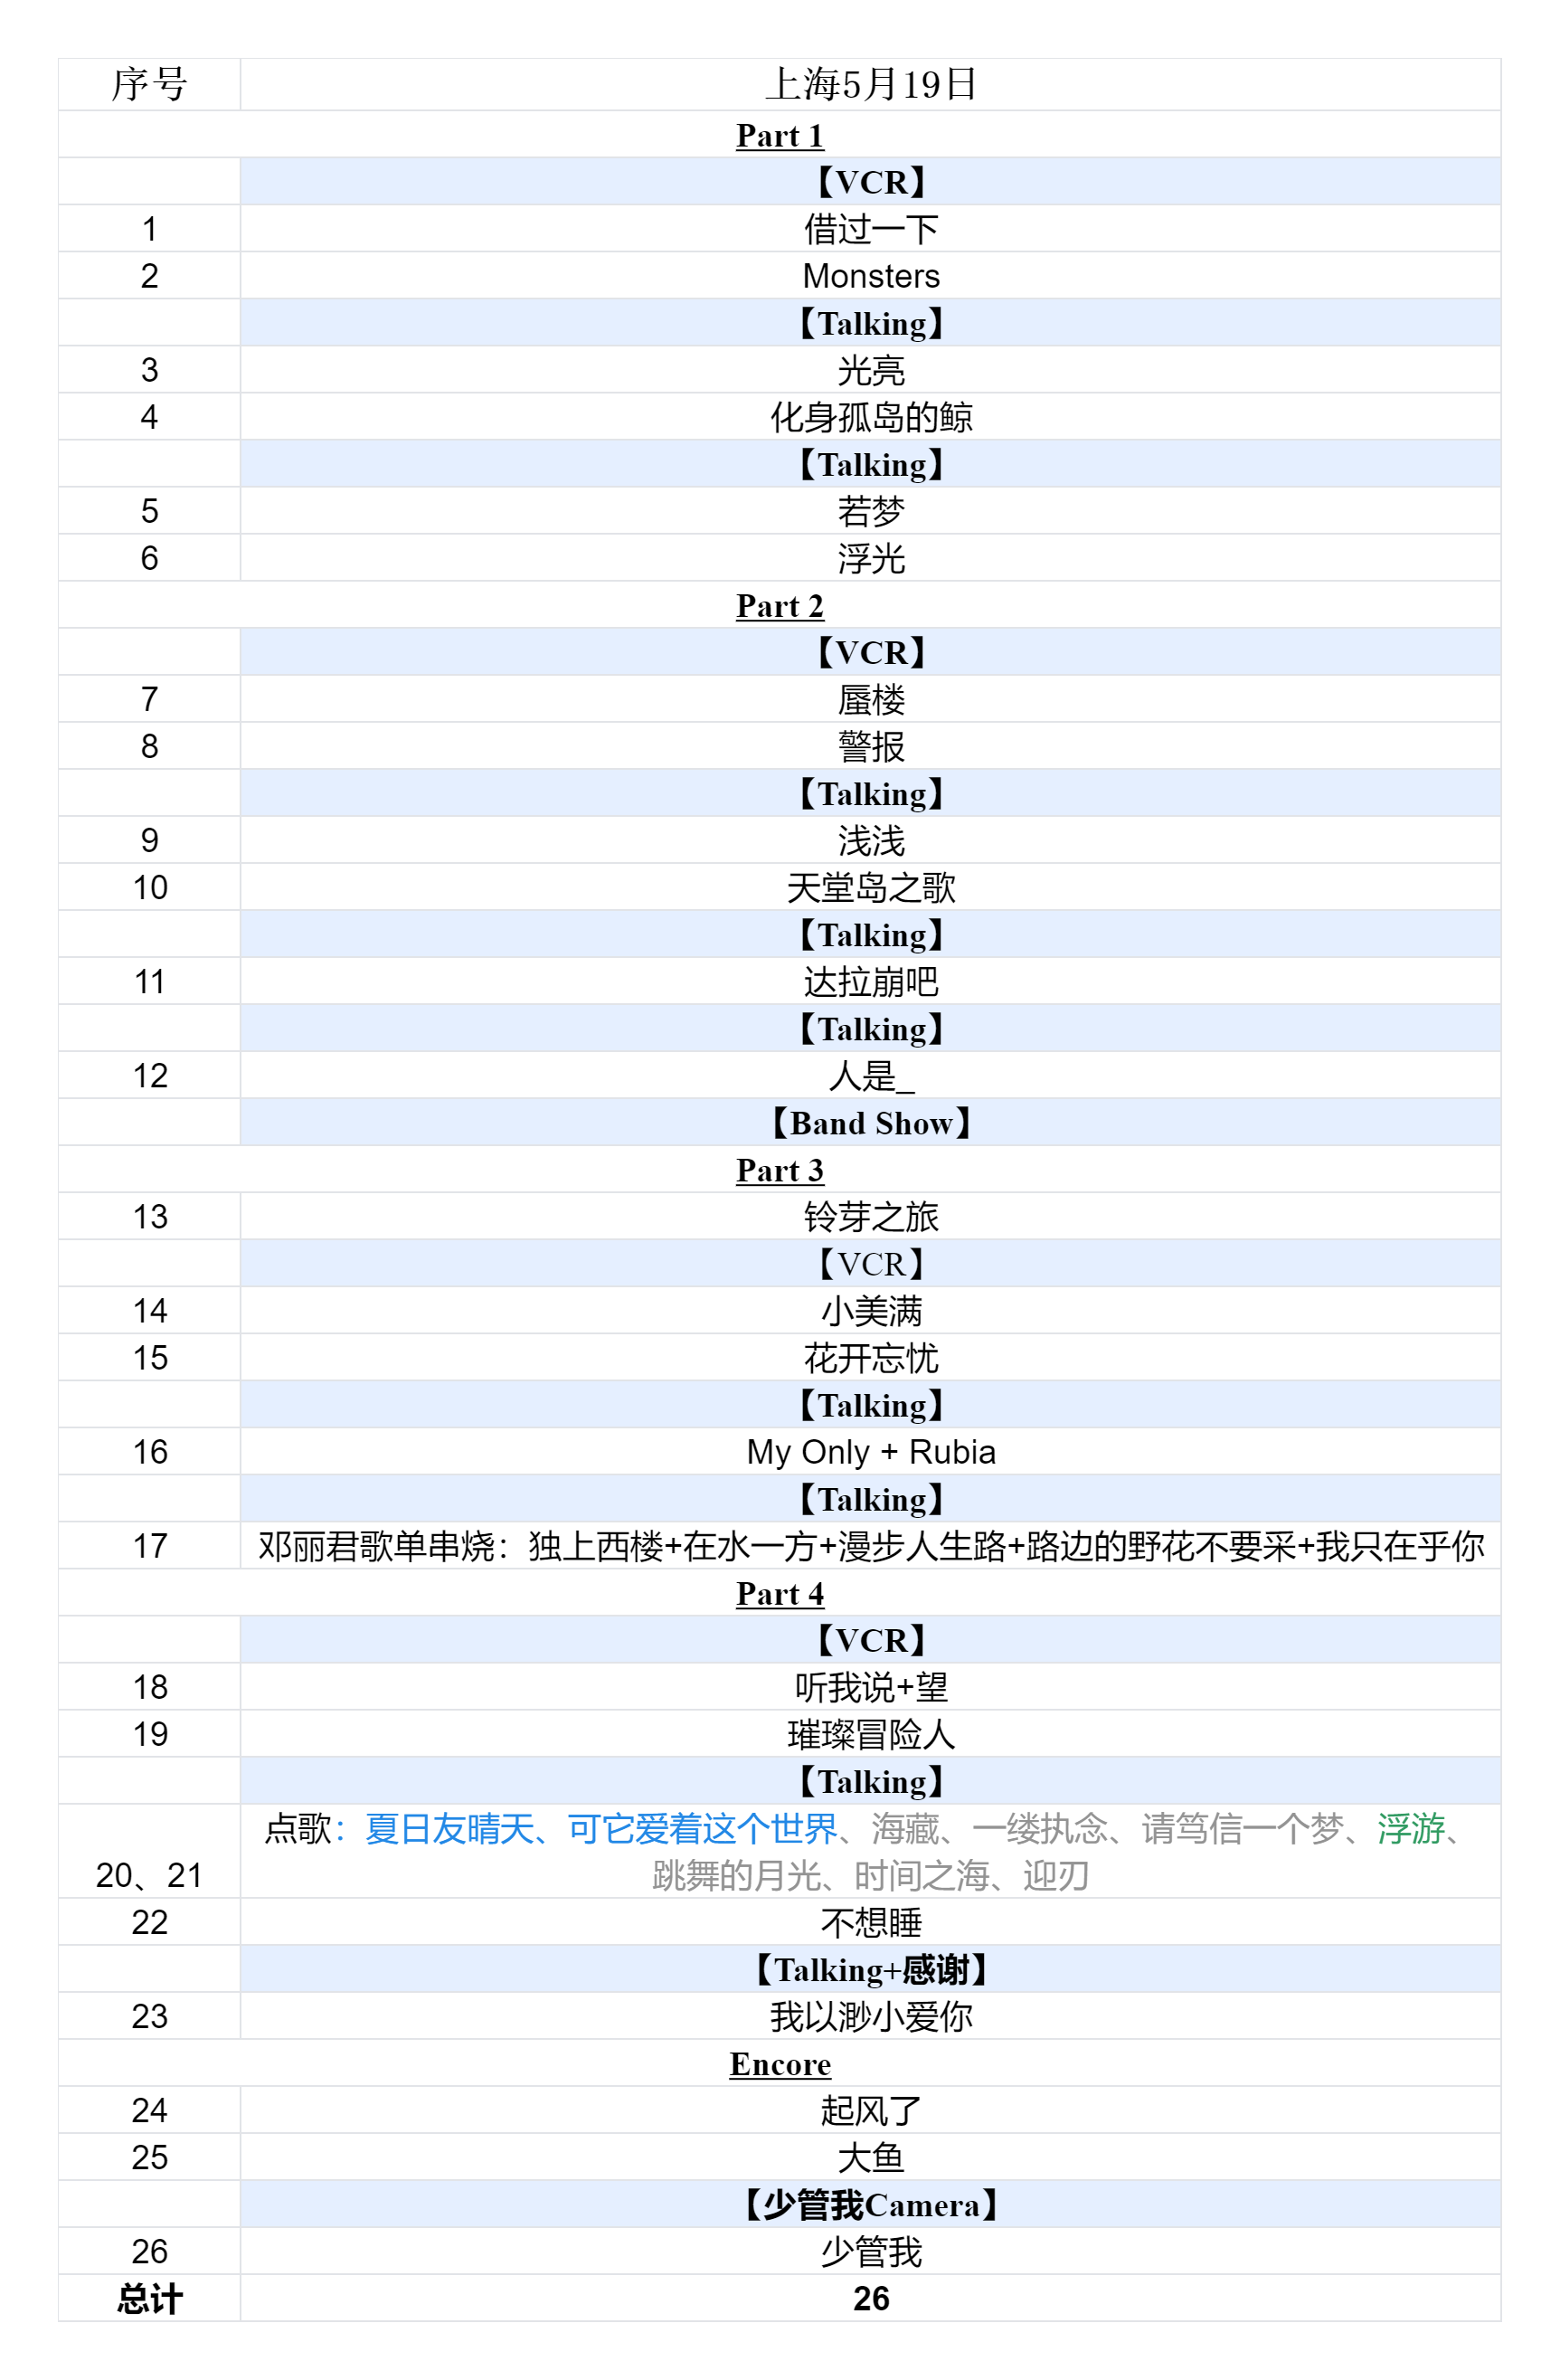
\includegraphics[width=320pt]{img/playlists/playlists-shanghai-20240519} 

}

\caption{2024周深9.29Hz巡回演唱会2024.05.19上海第二场歌单}\label{fig:unnamed-chunk-38}
\end{figure}

\newpage

\section{Part1}\label{shanghai-20240519-part1}

\hyperref[opening-vcr]{🎥【\textbf{开场VCR}】}

\hyperref[I-will-go-my-way]{🎵【\textbf{借过一下}】}你们好吗?

\hyperref[Monsters]{🎵【\textbf{Monsters}】}

  上海的朋友们,你们好吗?很开心终于跟大家见面了啦,此处特别适合说一句,\textbf{我想死你们啦。}现在用我们的掌声欢迎钱雷老师,好,给大家介绍一下自己吧?我已经介绍过你了,来吧,给大家打个招呼。(钱雷:hello,大家好,我是深深最好的朋友)怎么这个比较级,比昨天又更高了一级,哈哈哈。好,那这首歌依然是非常治愈,然后也是雷哥写的一首,也是我自己很喜欢的一首流行跟咱们的戏曲结合的非常感人的一首歌,你们知道是什么歌吗?(米:光亮)好,希望你们喜欢这首歌,光亮。

\hyperref[silver-linings]{🎵【\textbf{光亮}】}

\hyperref[hua-shen-gu-dao-de-jing]{🎵【\textbf{化身孤岛的鲸}】}你们会吗?(米:会,你的衣衫破旧,而歌声却温柔,陪我漫无目的的四处漂流\textasciitilde)你们唱得真好听\textasciitilde 到你们\textasciitilde 这边\textasciitilde(深:我想给你能奔跑的岸头)(米:没有墙头)我不信,我也依然还要唱(深:无论你们有多少个墙头,你们也是国王和王后)谢谢大家\textasciitilde{}

  大家好,我是周深,你们好吗?(米:好)好,到了我们明目张胆的换衣服时间,\textbf{非常非常非常非常兴奋再次见到大家,因为我觉得我已经太久没有见到了,你们想我吗?(米:想)}真的想的告诉我一下,真的想吗?假的想的告诉我一下,假的想的可以从绿色那个安全出口出去一下。然后这次巡回演唱会的主题是(米:9.29Hz),没错,因为是跟我自己性格比较像,我觉得自己可能,我性格比较内向,为什么会有人笑得这么大声?哈哈哈,我在换衣服,我的耳机突然传来啊哈哈哈哈\textasciitilde 我在认真的介绍我们的主题,9.29Hz,\textbf{我一直觉得自己是一个,应该说是不会被听到的一个像次声波这样的存在,但是谢谢你们每个人听到了我的声音,让我慢慢可以从一个个舞台走到你的面前,非常非常感谢,也非常感谢你们选择我来治愈你们每一分每一秒,你们也都在治愈着我,让我这个曾经以为自己是孤岛的鲸的人,慢慢有一条路,去慢慢遇到更多同频的你。}谢谢你们,好吗?(米:好)你们是不是因为你们唱歌唱得很好,所以,嘿嘿,听着觉得我这个人唱的还不错。(米:哈哈哈哈)老师你笑声太大啦,哈哈哈,我是说很开心很开心听到这样的笑声,而且,哎呀,我觉得我想说的太多了,我还想继续听你们唱歌,你们愿意继续唱给我听吗?(米:愿意)那这首歌要跟我一起唱哦,(米:好)若梦。

\hyperref[ruomeng]{🎵【\textbf{若梦}】}(米:宝贝)宝你个头\textasciitilde 到你们(米:往事流转在你眼眸)这边,这边的朋友,前面的朋友大声点\textasciitilde(深:因为你我才得到拯救)

\hyperref[floating-light]{🎵【\textbf{浮光}】}你们等下愿意跟我唱这首歌吗\textasciitilde{}

\section{Part2}\label{shanghai-20240519-part2}

\hyperref[senself-vcr]{🎥【\textbf{反深代词VCR}】}

\hyperref[mirage]{🎵【\textbf{蜃楼}】}

\hyperref[the-giver]{🎵【\textbf{警报}】}

  谢谢大家,刚才那两首歌你们喜欢听吗?(米:喜欢)。谢谢大家,大家知道刚才那两首歌是哪里的歌吗?(米:反深代词)没错,是我新专辑反深代词的两首歌,反深代词说的是200年后的世界,可能科技会变得非常发达,所有的事情会便捷到我们无法去想象,所以我们就一直在思考,我们在思考那200年后变的东西那么多,我们有什么东西是没有变的,总是不停地去探寻,什么不变?爱我不变?哈哈哈,我要是信了你们,我应该不会有今天吧,哈哈哈,就是我们在探寻人跟人之间的羁绊,或者是所有那些所有我们可能困惑的东西,或者喜欢的、享受的、开心的东西。所以也希望大家可以走进那个200年后的世界,一起去寻找一下那些属于我的碎片,因为每首歌都是我的化身,也有可能可以找到非常像你的那一块碎片,好吗?(米:好)好的,那接下来这首歌跟我的名字是相反的,所以它叫(米:浅浅)。就我之前立过很多flag,都倒了,以前我绝对不会觉得别人称呼我为深深会很自然,啊,你喊我?以前总是别人喊我什么,深啊,我就会,啊,你能不能喊我全名周深,但是我觉得所有东西遇到你们都会发生改变,都会变得越来越好,所以谢谢你们,那这首歌也希望你们喜欢,浅浅。

\hyperref[qianqian]{🎵【\textbf{浅浅}】}(米:爱你)你爱的人太多,哈哈哈

\hyperref[haven-song]{🎵【\textbf{天堂岛之歌}】}

  今天演唱会到此结束,我没有逃出去。刚才那首歌你们喜欢吗?(米:喜欢),但是我真的会害怕你们回去不敢睡觉,有人被吓到吗?不要再逞强了。哈哈哈,那接下来这首歌我想要你们跟我一起唱,它是一个童话故事,它是什么歌呢?(米:达拉崩吧)你们现在回答的这么大声音,等一下不会放我鸽子吧?(米:不会)那我们试一下,(深:陛下,我叫)(米:达拉崩吧斑得贝迪卜多比鲁翁)哎呦,有点厉害哦,那我们等下来见真招。

\hyperref[dalabengba]{🎵【\textbf{达拉崩吧}】}等下要到你们喽,这个童话故事谁咬了谁?谁打了谁?谁又救了谁呢?于是\textasciitilde{}

  \textbf{我觉得我非常幸福,因为我拥有顶级的观众。}你们太棒了,然后你们相信你们也看到氛围非常好,也就知道了谁要来了,谁?(米:钱雷)哈哈哈,对,雷哥,好开心哦,大家掌声欢迎钱雷。好,给大家打个招呼吧,哈哈哈,(钱雷:大家好大家好,哈哈哈)大家熟悉钱雷吗?(米:熟悉)那还用我介绍吗?(米:要)也要?那就是说到这个作曲家,艺术家,非常著名的作曲艺术家,一定要说到他的作品。比如爱你(米:孤身走暗巷)啊,停,然后再来,(深:祝你踏过)(米:千重浪能留在爱人的身旁)好,停,不能唱多了,还有一首,你自己想听他们唱哪一首,(钱雷:爱你孤身)好,今天比昨天更腼腆了,原来欺负i人还能一天比一天快乐,哈哈哈哈哈哈。(昨天不是把话筒给我了嘛,还敢再给一次吗?)下面有请钱雷为大家演唱人是\_。(钱雷:看我把手机打开,因为当时他前段时间发给我,他自己写的一首歌),朋友就是这样吗?就是这么的彼此信任,彼此互相给对方挖坑,但是我们关系真的很好,那每次唱这首歌我都会很想问,这首歌叫人是,每次唱我都觉得,``雷哥,你是人吗?''哈哈哈,谢谢你的回答,那这首人是\_希望你们喜欢。

\hyperref[renshi]{🎵【\textbf{人是\_}】}掌声感谢雷哥\textasciitilde{}

\section{Part3}\label{shanghai-20240519-part3}

\hyperref[travel-lingya]{🎵【\textbf{铃芽之旅}】}

\hyperref[close-door-vcr]{🎥【\textbf{关闭客服大门VCR}】}

\hyperref[happy-ending]{🎵【\textbf{小美满}】}愿意跟我一起唱这首歌吗?那我就放心交给你们喽\textasciitilde 大声点\textasciitilde 一起\textasciitilde 哇,谢谢大家,体验到了伍佰老师的快乐,再大声点哦\textasciitilde 后面朋友,大声点\textasciitilde 谢谢在座的每一个你,或者是没有到现场的,\textbf{让我觉得我们生活中一直都充满了幸运,充满了非常非常多的小美满。}每次一听这首歌,有人会告诉我很治愈,很开心,但是总给我一种感觉,许的愿望能成真。所以我希望大家在接下来短短的时间里,能够相信彼此,我们一起在这里许愿。比如我先许一个愿望,321,我的愿望就会挂在那里。所以现在无论你年纪大小,无论你是几几年生的,希望大家都可以听我的话,我们现在把眼睛闭上,默默许一个愿望,好吗?答应我,快闭上眼睛,默默许个愿望,想好那个愿望,但是有一个要求,那个愿望必须是关于自己的,就像这个小美满,我们要好好的爱好自己,自己都是非常珍贵,非常美好,一直也在治愈这个世界,准备好了,321睁眼,你们的愿望都会被听见\textasciitilde{}

\hyperref[no-worries]{🎵【\textbf{花开忘忧}】}(深:若记忆被偷走了,忘了我的爱,我会说)(米:你好啊)你好啊\textasciitilde 愿意和我一起吗?因为你们,每一朵忘忧草都开花了。谢谢大家!

  我想说,今天有没有人是第一次来听我演唱会?(米:有)哇,哈哈哈,好开心好开心,因为我自己也是从一个歌者变成一个歌手,所以我知道要下定决心去看演唱,然后买到票,然后去看演唱会,其实需要去花费自己非常多时间跟精力。(米:加场加场)哈哈哈,你们知道吗?\textbf{票难买对我来说也是一个,对我来说从来没有想过的小美满。}所以我觉得,你一定要相信自己的实力,真的让一个非常平凡、非常普通的人慢慢站上了这个舞台,所以要相信自己好吗?(米:好)不够大声,相信自己好吗?(米:好)要记住你们刚才在小美满许的那个愿望,都要关于自己的哟。

  那接下来这两首歌我觉得是非常非常幸福,非常浪漫的两首歌,之前听过我演唱会的也都知道,会弹琴,哈哈,但是我努力,我加油,希望你们能够喜欢这两首歌。你们有没有看到这个舞台是非常非常漂亮的,像一颗树的样子。对,然后你们,应该是每个位置上也都会有一个可以种的种子,对不对?(米:对)\textbf{你们都可以回去种一下,就算是我们演唱会的一个美好记忆的一个延续。}当然我也知道有人会觉得害怕自己种不活。不用害怕,这个事情在我身上发生了四次,哈哈哈,四次都是别的老师跟我说,你去养,很好养活的,然后我每次养的时候都不行,我问老师,谁告诉你它很好养的?就可能是,大概三天浇一次水的,我一天浇了三次水。但无论怎么样,我觉得大家都可以种下,好吗?(米:好)那是我们的延续哦,加油,好的,我会加油的。

\hyperref[my-only]{🎵【\textbf{My Only}】} 我才弹这么一点点的时候,你说太棒了会不会有点假\textasciitilde 记错词了对不起(米:哈哈哈哈哈哈,没关系)再给我一次机会\textasciitilde{}

\hyperref[rubia]{🎵【\textbf{Rubia}】}\textbf{谢谢你们愿意看见这个不完美的我,愿意去接纳我的每一个碎片,请相信我,我也是!我们都是最棒的\textasciitilde{}}

  谢谢大家。比较熟悉我的朋友知道,算是对我的声乐启蒙的演唱家是谁?(米:邓丽君)没错,有人喜欢她吗?(米:有)我相信应该每个人都听过她的歌,对不对?你们都特别喜欢她的哪首歌?因为现在来到了,怎么说呢?就是这个非常棒的点歌台,你们想唱的歌我都会点,你们想听哪首歌?欢迎邓丽君女士的,你们点的再多都是没有用的,因为我已经编完曲了,希望你们喜欢这个串烧。

🎵【\textbf{邓丽君组曲}】
\hyperref[one-in-the-building]{🎵【\textbf{独上西楼}】}来来来,9号桌的朋友你要听哪首歌?好的
\hyperref[on-the-water-side]{🎵【\textbf{在水一方}】}
\hyperref[walk-the-road-of-life]{🎵【\textbf{漫步人生路}】} 大声点\textasciitilde 希望你们给我最热烈的掌声,好吗?(米:好啊啊啊)
\hyperref[only-with-me]{🎵【\textbf{路边的野花不要采}】}那些墙头多的人,给我藏好了(深:路边的野花,你不要采\textasciitilde)全场\textasciitilde{}
\hyperref[only-you]{🎵【\textbf{我只在乎你}】} 谢谢你们\textasciitilde{}

\section{Part4}\label{shanghai-20240519-part4}

\hyperref[thank-you-vcr]{🎥【\textbf{谢谢上海,谢谢你VCR}】}

\hyperref[listen-to-me]{🎵【\textbf{听我说}】} 到你们(米:听我说,可以听我说)谢谢你们总和我说,谢谢你们,谢谢你。

\hyperref[hope]{🎵【\textbf{望}】}交给你们(米:我们总会绕啊绕,绕啊绕\textasciitilde)

\begin{figure}

{\centering 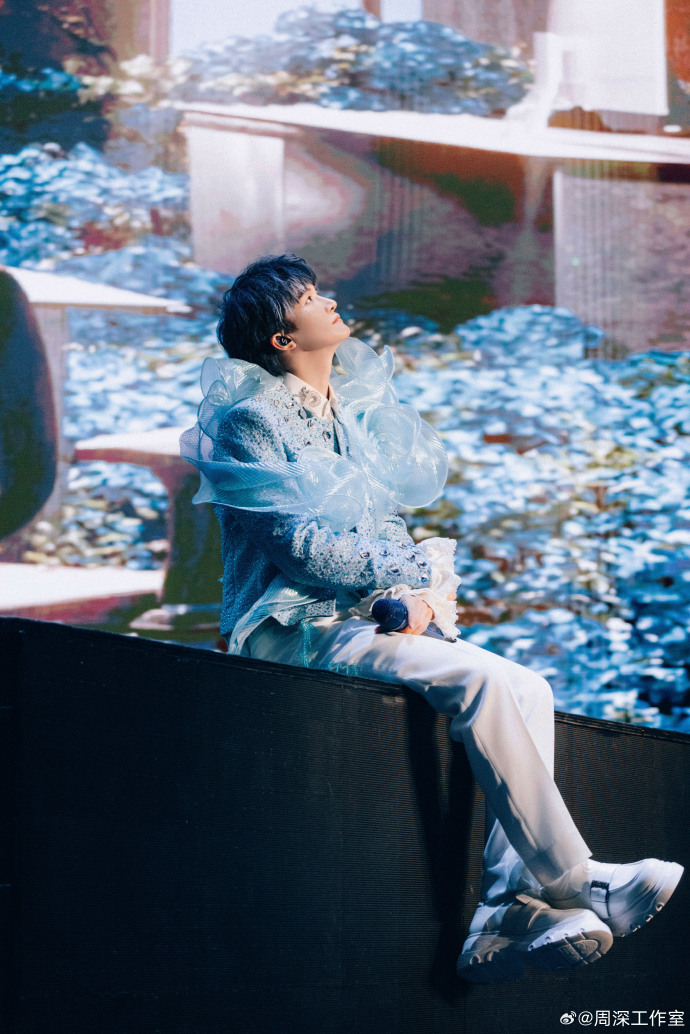
\includegraphics[width=400pt]{img/shanghai20240519/001} 

}

\caption{上海519听我说}\label{fig:unnamed-chunk-39}
\end{figure}

\hyperref[adventurers]{🎵【\textbf{璀璨冒险人}】} 谢谢大家,谢谢老师们\textasciitilde{}

【\textbf{点歌环节}】诶,宝你个头,我自己也很喜欢看音乐节或者看演唱会,就发现,诶,别人点歌的环节我们也要有,所以,接下来是属于我们的点歌环节,但是,宝你个头宝你个头宝你个头宝你个头,但是今天的点歌环节有一点点特殊。因为,就如果我今天不是在开演唱会,我今天应该是在东北录跑男,然后他们今天,我居然错过了泥潭环节,我居然错过了在东北玩泥巴,这么好的契机,在东北玩泥巴,居然错过了,但是我的跑男兄弟们,他们说他们想见见大家。(跑男团:想你了。很羡慕这个现场抢到票的朋友。就是不像我们没抢到票的人,只能来录制跑男,给姚PD做牛做马。谢谢来到现场的朋友们对深深的支持,谢谢大家)谢谢大家(深深刚刚发布了新专辑,新歌叫少管我,少管我们深深。太想你了深哥,祝你巡回演唱会圆满成功,我们在家里等你。跑男合唱:你快回来\textasciitilde)唱歌好不整齐的\textasciitilde(但是你们还有一个任务需要完成,今晚的演唱会还有一个点歌环节,你们也要参与其中,而你们点歌的方式很特别,请来领取歌单)大家跟他们打个招呼,123,嗨(米:嗨)他们怎么可能会看得见,有人想听这些歌吗?一缕执念有人想听吗?时间之海有人想听吗?可它爱着这个世界有人想听吗?夏日友晴天有人想听吗?那我们看一下我们的跑男兄弟们会选哪一首,很有趣味的一个点歌方式。(我是金典款,准备好了吗?好了,321)哦,不会是谁抽到第一就唱哪首歌吧?沙哥不想听我唱歌,沙哥又飞回去了。(后天见,奔跑吧,周深)谢谢谢谢,谢谢我们跑男兄弟团,我们一起到这里喊一个奔跑吧好不好?321(米:奔跑吧)耶,然后他们好像,除了今天玩泥潭之外,今天还撕名牌,我绝对不是这一季第一个被撕的,因为两次撕名牌我都错过了。那我们就来唱这首可它爱着这个世界吧,你们想听吗?(米:想)要跟我一起唱哦(米:好)。

\hyperref[love-the-world]{🎵【\textbf{可它爱着这个世界}】}哈喽\textasciitilde 谢谢

  谢谢我们跑男团兄弟们,也希望他们今天撕得开心,没有我的日子,找不到人要撕谁了吧,我跟你们说,每次跑男团,一撕名牌,包括飞行嘉宾,别人都是,嗷\textasciitilde 齐刷刷的看向我,我每次告诉他们,\textbf{我不是那么好撕的,我跑得快呀。}

  那这个点歌机会,当然也依然有我们现场观众的朋友们啦。老规矩,然后我们的摄像老师,请你疯狂的摇摆,请你跟我们一起摇摆,然后我喊321后,定到谁,你就拥有点歌的权利,看一下有没有喜欢的歌,我们来找一找,5(米:4321),哇,小朋友你好。你在哪啊?啊,你在这,怎么称呼你?陈玉林?欢迎陈玉林小朋友,你是哪里的?哦,我不用跟他喊那么大声,你是哪里的?上海的。哦,你是上海的小朋友,那上面有你想听的歌吗?你,你还真的是从小就听我的歌呢,你现在几岁啊?10岁,哦,放假了吗?哦,今天周末是吧?好,我放过你这些恶魔问题,哈哈哈,你最喜欢下面哪首歌啊?夏日友夏天,小朋友再认真读一次,哈哈哈,不会,玉林小朋友,你想听哪首歌?夏日友晴天,谢谢玉林小朋友,那就带来这首充满童趣,也是跟我们,迪士尼也在我们上海,对不对?大家都有去过吗?(米:有)\textbf{让我感觉所有东西都会被治愈,这首歌里面也会治愈你的一切},谢谢玉林小朋友,特别的巧,小朋友点的一首充满童趣,充满欢乐的夏日友情天,送给每一个小朋友、大朋友。新生产的机器就是好,声音一喊就透亮。昨天有个小朋友,我问他叫啥,我小抖,最后她原来叫小董。

\hyperref[sunny-day-in-summer]{🎵【\textbf{夏日友晴天}】}摇起来\textasciitilde{}

\hyperref[keep-playing]{🎵【\textbf{不想睡}】}来,大声点\textasciitilde 谢谢你们\textasciitilde 大声点\textasciitilde{}

  \textbf{谢谢大家,谢谢大家来看我,谢谢大家愿意听见我,谢谢你们的光,相信自己力量非常大},是不是刚才听到一个人破音破得很严重,我其实听得很清楚,但是我要假装冷静,毕竟我今天是站得最高的人,哦,不对,还有我们看台的朋友们站得比我高,看台的朋友们你们好吗?我们能够平安的开心的一起去创造美好的回忆。我们也要谢谢非常非常多给我们大力支持的朋友们,先掌声给所有支持我们的朋友们。

  首先非常感谢场地支持梅赛德斯奔驰文化中心,用最热烈的掌声感谢上海市公安局治安总队、上海市公安局浦东分局、上海市文化和旅游局、上海市文化市场行政执法总队、浦东新区文化体育和旅游局、上海市消防救援总队,以及感谢浦东新区消防救援支队,以及其他部门的大力支持,让我们很开心的平安的相见,也要非常感谢本次巡演的全程主办,北京时代立方文化传播有限公司,我有问过我们这个主办方的朋友,就是说怎么会想给我开演唱会,特别巧,他们是在几年前,5月18号,有一场我跟黄龄老师演唱会,叫深临其境,那个时候有人在听吗?那一场演唱会他们听了那一场,他们觉得,哎呀这个小伙子看起来不错,没有,哈哈哈,他不是这个口音,哈哈哈,所以他就觉得我是能够被大家看见,因为他觉得有很多人看到我,不想辜负你们的努力,所以让我慢慢慢慢跟大家相见,非常非常感谢他们,谢谢。也感谢上海站协办TME Live腾讯娱乐超现场,感谢演唱会制作单位必应,感谢我们的总导演周佑洋、庄惟惞。然后这位我要非常非常感谢,也是我非常感动地,从看着我出道到现在,然后一直应该说是每次需要帮助或者自己没有信心的时候,总是会给我鼓励的音响总监金少刚老师,大家今天听我的声音还好听吗?(米:好听)都是金少刚老师给的,要感谢音乐总监龙隆老师,以及感谢我们今天所有的乐队老师们,感谢我们的合唱老师们,以及还要感谢我们的钱雷老师,他在后台,可能要大声点。感谢钱雷老师,好偏心啊,等下你们感谢我有没有那么大声。以及感谢舞蹈团队SDT ShowPro,以及感谢我们服装团队设计师劳伦斯许工作室,以及时装品牌Windowsen,sensen。感谢音响工程南京奥斯泰视听科技有限公司,感谢调音团队乐尔工作室,感谢硬体工程北京力超舞台集团。大家看,我多幸运,每次与你们相见,后面有这么多老师为我去加油,然后打气,去建造这样的舞台,跟大家见面,我真的很幸福,然后也要感谢周深工作室的小伙伴们,好的好的好的,我们很开心,感谢票务总代理大麦网(米:倒闭)调皮,感谢票务代理猫眼票星球(米:倒闭),感谢微博,感谢微博音乐,感谢微博演出,要大声点感谢他们。以及感谢所有的工作人员,当然\textbf{最最最最重要的感谢我的生米,感谢布丁,感谢每一个来到这里的你,谢谢你。}

  知道卡布的会知道,不想睡其实是最后一首,但是,接下来这首是属于周深的晚安曲,我以渺小爱你,但是在此之前大家来合一张照好不好,(米:好)好了好了,来中间的先,321,你看我pose多就知道我也是拍过时尚杂志的人,哈哈哈。左边的朋友,321,右边的朋友,321,谢谢,我以渺小爱你。

\hyperref[loving-you-in-my-humble-way]{🎵【\textbf{我以渺小爱你}】}\textbf{谢谢你们有一个温柔的灵魂。}

\section{Part5}\label{shanghai-20240519-part5}

\hyperref[the-wind-rises]{🎵【\textbf{起风了}】}你们好吗\textasciitilde 谢谢你们,愿意和我一起,谢谢你们\textasciitilde(深:以爱之名,你还愿意吗)(米:愿意)

\hyperref[big-fish]{🎵【\textbf{大鱼}】}我也希望你们天天开心\textasciitilde 谢谢大家\textasciitilde{}

  这也就意味着我们今天演唱会就要结束喽,大家听得还开心吗?(米:开心)没错,我有一个三个字比较出圈的话,叫做(米:少管我),我们演唱会上面有个少管我camera,camera就是摄像机。也就是说,这个摄像机如果抓到谁,捕捉到了谁,哈哈哈,我们来抓,这个摄像捕捉到了谁,放大之后,你要做少管我的专属姿势,嘿,少管我,这也是我新专辑反深代词里面的一首歌,大家听了吗?(米:听了)那全场,我们先预习一遍,嘿少管我,好不好?321,嘿,少管我。没错,很好,今天打到前排朋友的头的人比较少,哈哈哈,昨天我看到,他很激动,跟我们一起嘿少管我的时候,这个荧光棒飞到了前排,所以要注意安全,再来一遍321,嘿,少管我,我们把所有不开心的事,所有的烦恼全部都喊出去,好不好?(米:好)我们还是一样的,我们全场倒数五个数字,拍到谁,就要用你最大的声音喊出来,来,5(米:4321),朋友你好,你在哪里?哦,在那里,哈喽,你们两个是一起来的吗?是吗,那请问两位谁来喊呢?那么就女生吧,女生怎么称呼你?全然不知发生了什么事情,现在到你来喊少管我喽,怎么称呼你?宝?毛?矛?猫?帽?喵\textasciitilde 等一下,配合一下,来,321,宝?宝你个头,马?等一下,包?啊,你好你好,要弄清楚你的名字好难好神秘,好,你要准备用最大的声音喊出少管我配合姿势,等一下,你在哪里,哦在这里,要最大声哦,配合姿势,嘿少管我,321,非常完美。

  好,我们来下一个,再下一个,全场5,(米:4321)好,放大放大,就是你,哈喽,你在哪里?好,怎么称呼你?人?好巧,我也是人,你从哪里来的?从这里来的?安徽?哦,谢谢你,好了,喊出最大声音哦,321,非常好,我们全场再来一次,321,(米:嘿,少管我)

\hyperref[watch-ur-manners]{🎵【\textbf{少管我}】}来喽\textasciitilde 来喽,(米:嘿,少管我)要大声点哦,54321,(米:嘿,少管我)太棒啦\textasciitilde 你们的动作\textasciitilde 来喽,(米:嘿,少管我\textasciitilde)321,走(米:嘿,少管我\textasciitilde)谢谢大家听得见我,希望这个快乐轻松的结尾给你永远带来好心情,谢谢大家。谢谢你们,谢谢你们给了我一份非常美好、非常欢快的回忆。再来,321(米:嘿,少管我)你们太棒啦啊啊啊啊\textasciitilde 再次感谢到来的每一个你,谢谢你,哈喽后面的朋友,这边看台的朋友,谢谢,谢谢你,谢谢后排的朋友以及看台的朋友,谢谢,谢谢你们。谢谢后面的朋友,谢谢后面看台区的朋友,你好,谢谢,以及我们左边这边朋友你们好吗?大家回家注意安全,手机不要掉了看台的朋友,手机不要掉了,身份证不要掉了,人要平安安全回到家,好吗?(米:好)谢谢你们给我的快乐,我也希望能够给你们所有的快乐,谢谢你们。321,最后一次,(米:嘿,少管我)注意安全注意安全。

\begin{center}\rule{0.5\linewidth}{0.5pt}\end{center}

\begin{figure}
\centering
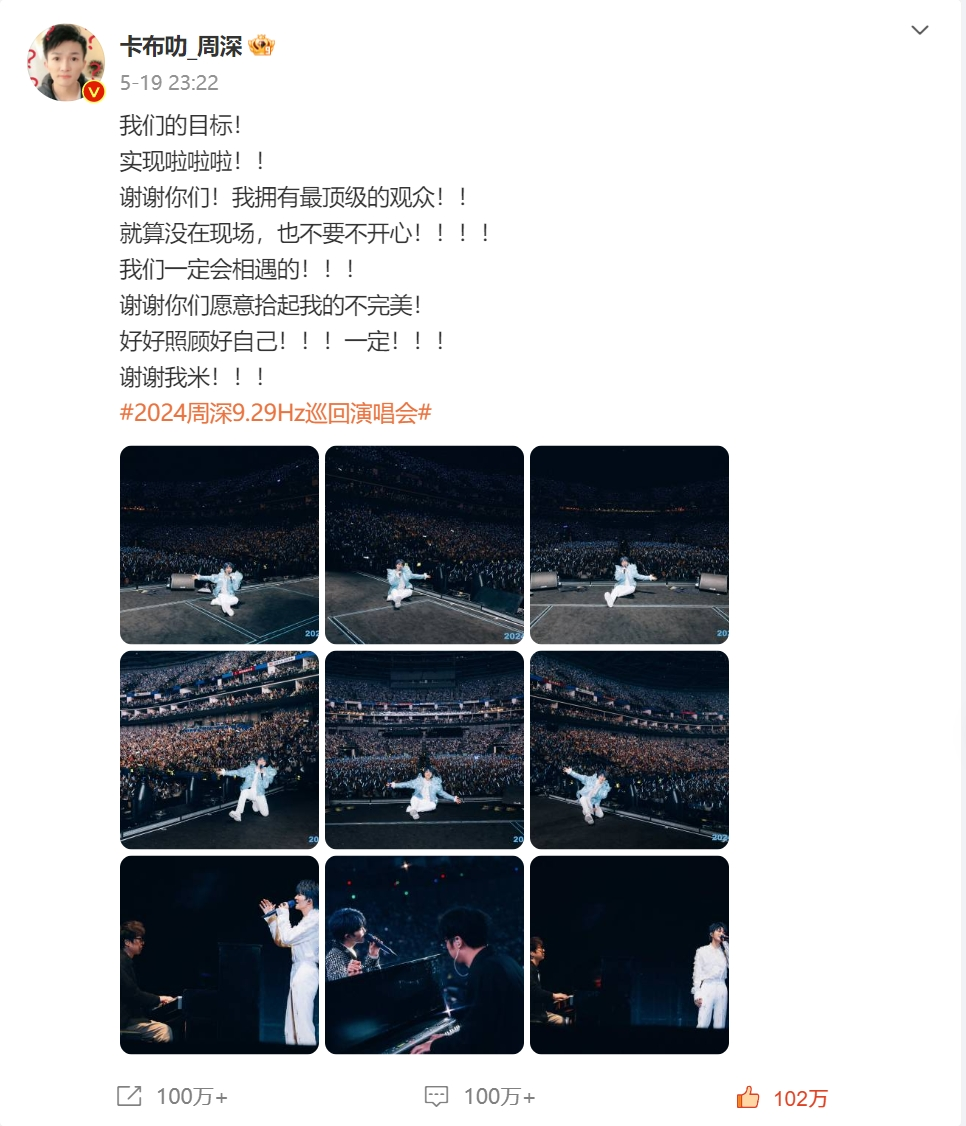
\includegraphics{img/weibo/shanghai-20240519.png}
\caption{\label{fig:unnamed-chunk-40}周深上海梅赛德斯奔驰文化中心演唱会结束微博 【\citet{weibo-charlie}】}
\end{figure}

\chapter{2024.06.01深圳场}\label{shenzhen-20240601}

\begin{quote}
\textbf{\emph{永远都不要忘记一颗糖就可以给你带来的快乐。------ 周深}}
\end{quote}

\begin{figure}

{\centering 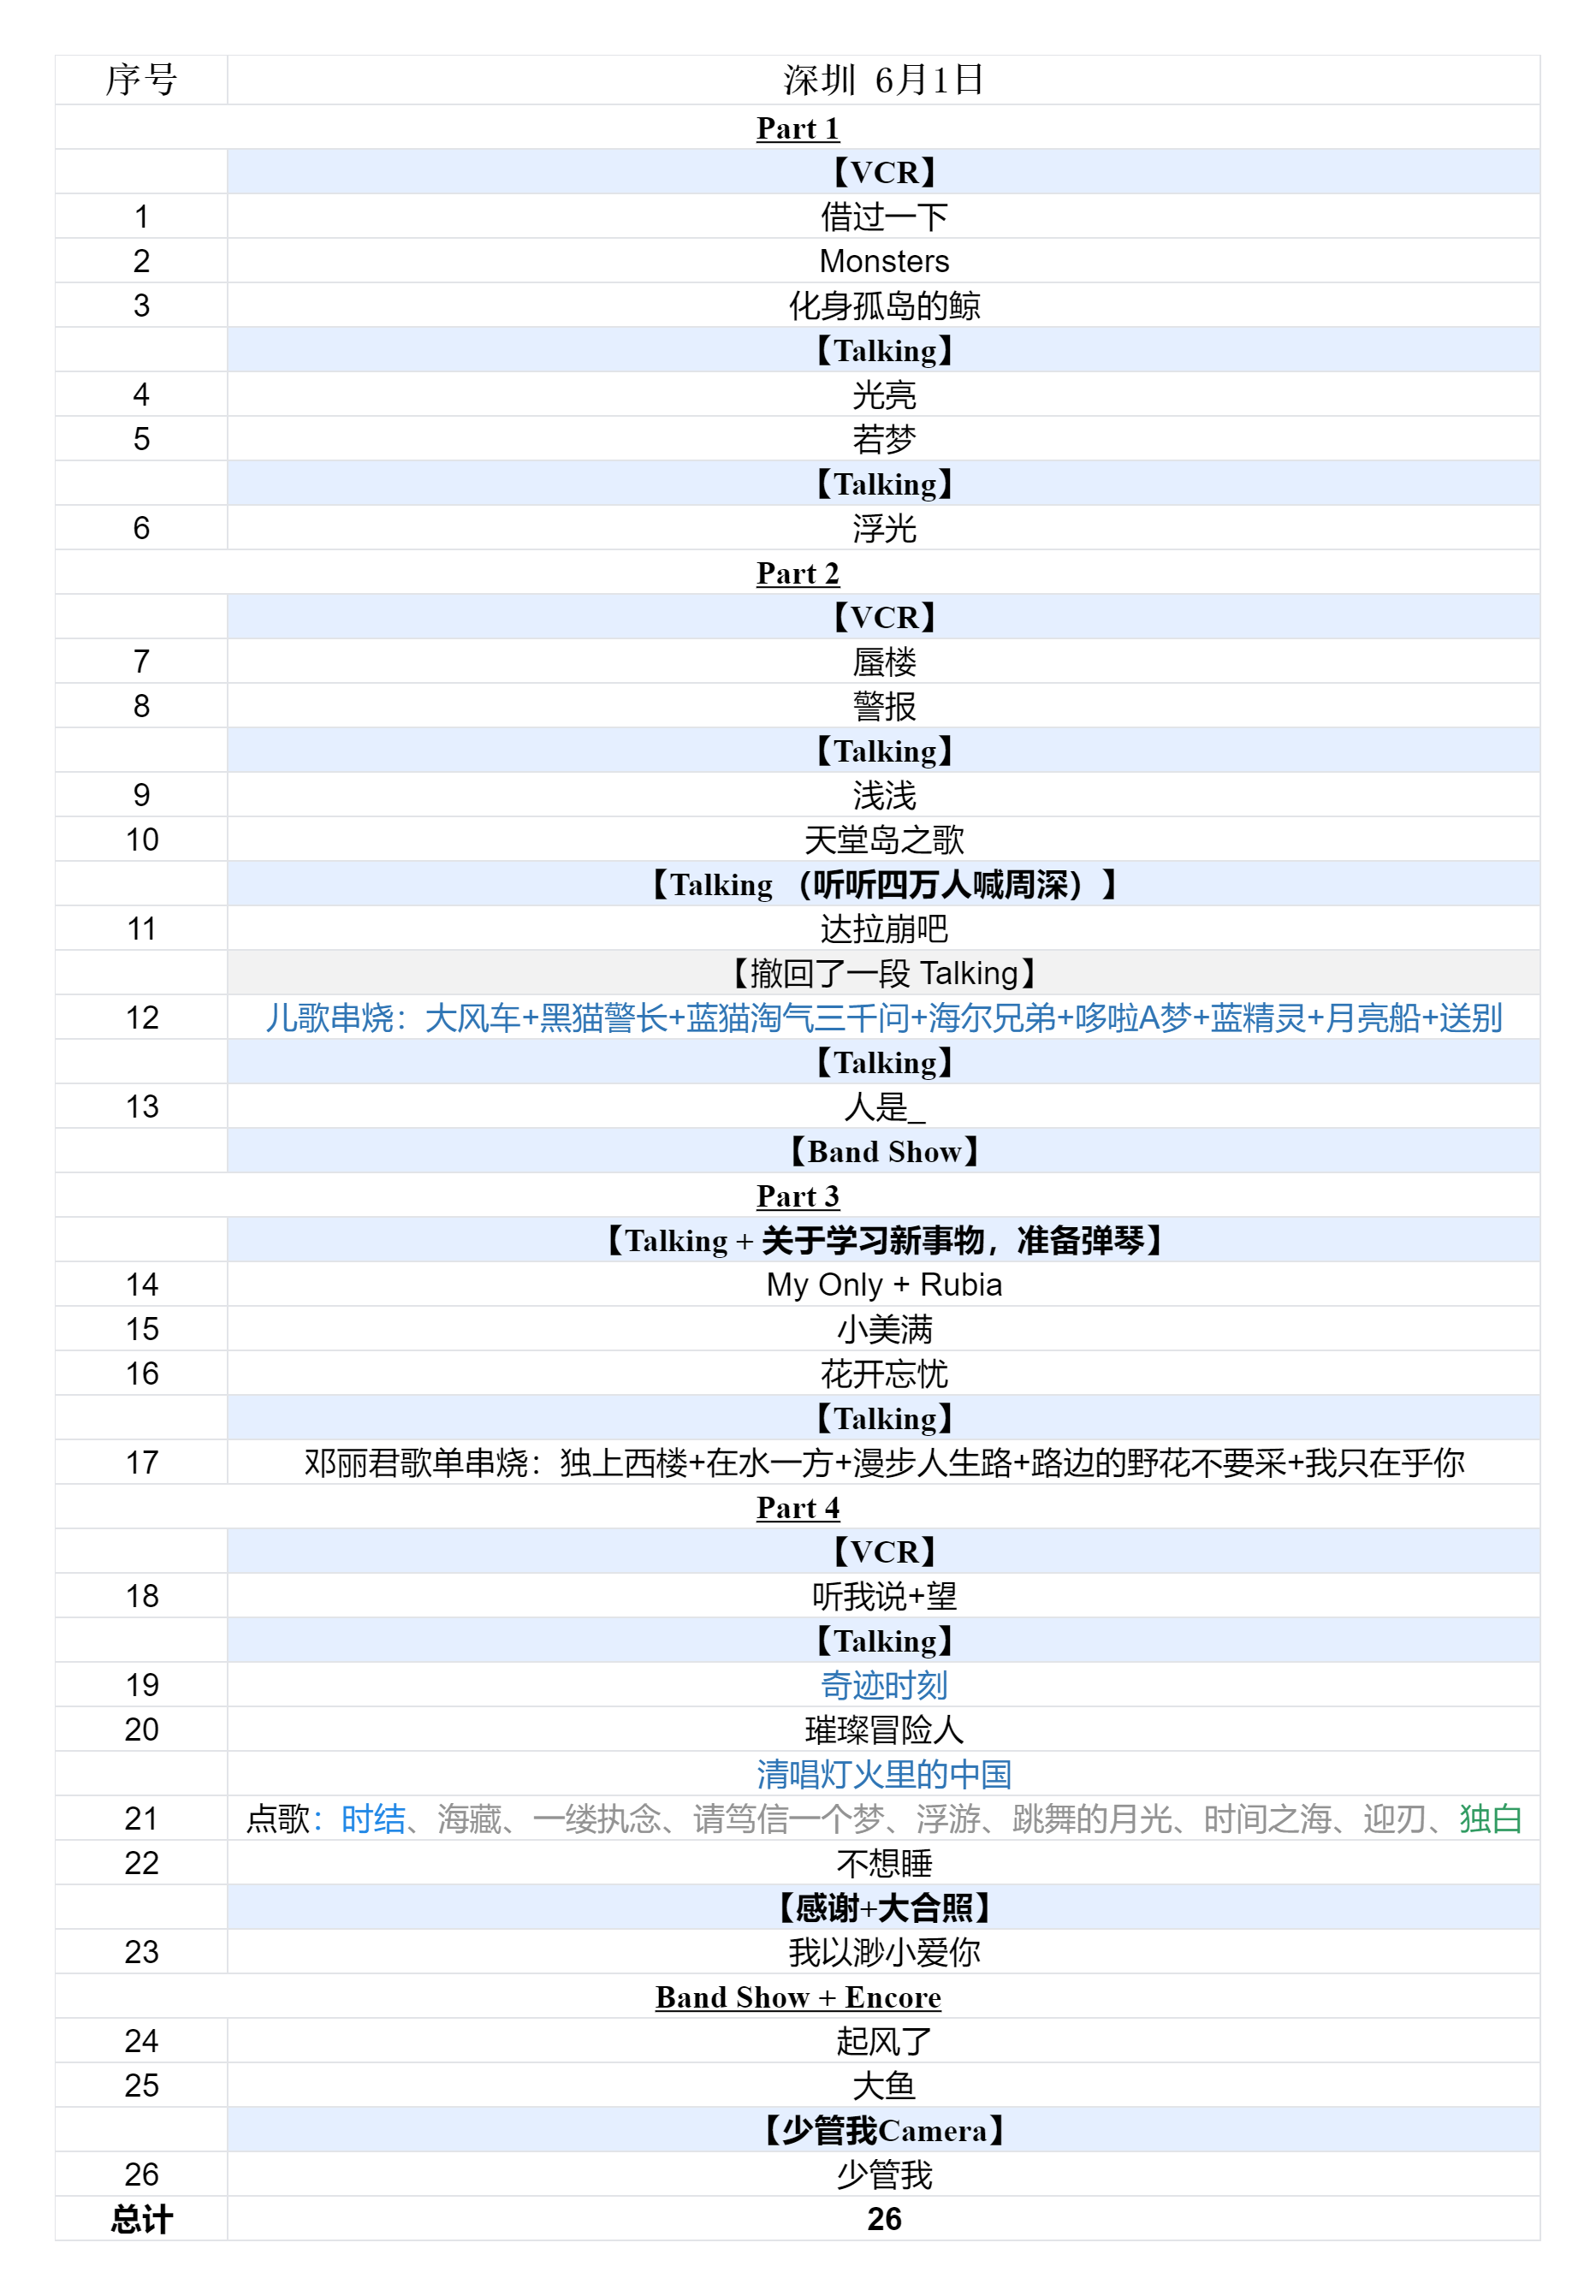
\includegraphics[width=320pt]{img/playlists/playlists-shenzhen-20240601} 

}

\caption{2024周深9.29Hz巡回演唱会2024.06.01深圳场歌单}\label{fig:unnamed-chunk-43}
\end{figure}

\newpage

\section{Part1}\label{shenzhen-20240601-part1}

\hyperref[opening-vcr]{🎥【\textbf{开场VCR}】}

\hyperref[I-will-go-my-way]{🎵【\textbf{借过一下}】} 你们好吗?(米:好)

\hyperref[Monsters]{🎵【\textbf{Monsters}】}

\hyperref[hua-shen-gu-dao-de-jing]{🎵【\textbf{化身孤岛的鲸}】}到你们\textasciitilde!谢谢你们\textasciitilde!到你们\textasciitilde 大声点\textasciitilde(深:我想给你能奔跑的岸头)(米:没有墙头)\textbf{大家好,我是卡布,我也是周深。}(深:让你如同王后\textasciitilde)

  深圳的朋友们,你们好吗!(米:好!)欢迎来到9.29Hz巡回演唱会,我真的太激动和太感动了。我先一边激动着一边感动着的换下衣服。首先,我辛苦化了两个小时的妆啊!(米:哈哈哈)其次,我不知道你们相不相信,刚出来的时候的周深,加上头发甚至可能高达一米六七!(米:哈哈哈)淋完一场雨之后,加上鞋可能一米六四!\textbf{还我的3厘米!}(怒音)(深、米:哈哈哈哈哈)但是我还是非常开心,而且我在刚刚,就是出场的时候朋友给我拍了一张照片,就是好像是有一位生米,然后他拄着一个拐杖走进来,然后一只手打着伞,一只手拄着拐杖走过来。然后我觉得特别特别感动,因为今天下雨嘛,很多时候大家第一反应就是,啊希望不要下雨。但到后面你接受它就好了,因为我觉得这场雨会让这一次相见变得更加的深刻。我只记得在小学的时候自己淋雨的记忆,是自己在放学的时候,然后爸爸妈妈因为很忙,所以你永远不会等来那一把撑过来的伞。但是现在我居然有这个荣幸,可以跟4万多人一起淋这一场雨!你们好吗?!(米:好\textasciitilde)\textbf{大家都说一起淋过雨的人可能永远不能忘记了,那完了,你们永远都不能忘记我啦!}(米:不会!)我的名字是?(米:周!!深!!)谢谢你们,\textbf{让我不再害怕,比这样更大的风雨我都见证过,而且你们都陪我一起见证过,谢谢你们愿意化作光亮去照亮我,因为你们永远是我心中的光亮。}谢谢你们!

\hyperref[silver-linings]{🎵【\textbf{光亮}】}谢谢你。

\hyperref[ruomeng]{🎵【\textbf{若梦}】}会唱这首歌吗?(米:会!)可以跟我一起唱吗\textasciitilde?到你们喽\textasciitilde(深:往事 米:流转\textasciitilde 在你眼眸\textasciitilde)大声点\textasciitilde(深:一边 米:遗忘\textasciitilde 一边拼凑\textasciitilde)(深、米:如我虔诚,合十双手\textasciitilde 唯愿你能得到拯救\textasciitilde)。你们唱的太好听了,谢谢你们\textasciitilde!要更大声哦\textasciitilde(深:往事)(米:流转\textasciitilde 在你眼眸\textasciitilde 一边遗忘一边拼凑)(深、米:如我虔诚\textasciitilde 合十双手oh\textasciitilde 唯愿你能\textasciitilde 得到拯救\textasciitilde)看台的!(深:往事)(深、米:流转\ldots\ldots 唯愿你能得到拯救\textasciitilde)(深:因为你们\textasciitilde 我才得到拯救\textasciitilde)谢谢。

\hyperref[floating-light]{🎵【\textbf{浮光}】}我没有想到我自己有那么多歌跟雨有关系哈哈,\textbf{我们每一次的相见,都非常的来之不易,非常感谢在这三万天当中,哪怕有一秒,你看见了我。}谢谢\textasciitilde!谢谢你们遇见了我,谢谢我能够遇见你们,谢谢你们!拜拜。

\section{Part2}\label{shenzhen-20240601-part2}

\hyperref[senself-vcr]{🎥【\textbf{反深代词VCR}】}

\hyperref[mirage]{🎵【\textbf{蜃楼}】}

\hyperref[the-giver]{🎵【\textbf{警报}】}

  刚才是我新专辑反深代词的两首歌,你们喜欢听吗?(米:喜欢)会不会稍微觉得,诶,好像跟印象当中的周深不太一样?声音那么那么小,是说很一样是吗?哈哈哈,原来我一直以为我是一个内向的、高冷的、古风的某唱歌男子,哈哈哈,但是诶,没想到我心中还有像我这张专辑这样的感觉,所以我觉得自己很幸福的是能够看到以前可能很多人印象当中的旧的周深,到现在可以慢慢开始表达一些很多人认为当中的新的周深,但是最幸福的是,哎,居然有人知道周深原本是什么样子,所以谢谢你们每一位,谢谢你们来看我,谢谢你们让我慢慢去寻找自己,谢谢你们。

  那接下来这首歌是我自己的第一张专辑的一首歌,你们应该知道是什么歌吧?诶,那我就要说一下了,因为自己以前别人叫我深啊,或者是什么,我都会很不习惯,我就很别扭,但是我也没有想到有一天我会习惯别人称呼我为(米:深深)深深。这首歌非常巧合,他在第一张专辑里面,但是他的风格跟二专的风格有一种莫名的相似。所以就是无论是旧的自己还是新的自己,一定都有一个自己在中间。这首歌叫浅浅,希望你能够喜欢。

\hyperref[qianqian]{🎵【\textbf{浅浅}】}

\hyperref[haven-song]{🎵【\textbf{天堂岛之歌}】}

  谢谢大家,大家好,刚才我在这首歌中间我指了一下下面。(深:叮咚,有人在看你),我觉得自己超酷、超吓人的,结果被我点到那个朋友,他拿着荧光棒,``哎,是我是我!''oh,好,要换衣服了,光明正大。今天是6月1号儿童节,大家有没有收到就是给你们的那一颗糖?(米:有),我觉得无论多少岁,或者是无论做什么工作,我们都可以是最开心的小朋友,对不对?(米:对)所以这颗糖,希望大家,怎么说呢?可以慢慢的在生活当中,可能我们一定要向上,一定要越来越好,可能要追求所谓的各种层面上的越来越好,但是也\textbf{永远都不要忘记一颗糖就可以给你带来的快乐},好吗?(米:好),永远要记住这份快乐。hello,看台的朋友们,哇,你们在离得那么远的地方,hello,hello,还有那边的朋友,内场的朋友你们好,hello hello,我想听一下4万多人一起喊我的名字是什么声音?321,(米:周深)。哇,这么好听的声音,等一下合唱这首歌一定会非常好听吧,哈哈哈。那如果等一下这首歌你们没有唱得这么大声,就要没收回那颗糖,开玩笑,哈哈哈,这首歌达拉嘣吧,你们准备好了吗?

\hyperref[dalabengba]{🎵【\textbf{达拉崩吧}】}接下来他们发生了什么事情呢,我们一起来揭秘一下吧。现在现场的朋友们,你们要想一下刚才那个故事,是谁打了谁?谁又咬了谁?最后故事到底发生了什么呢?\textbf{现在我想听各位小朋友们来告诉我},准备好了吗?于是\textasciitilde 砍向\textasciitilde 然后\textasciitilde 咬了\textasciitilde 最后\textasciitilde(深:要念你来念)我才不念(深:吧\textasciitilde)

🎵【\textbf{儿歌串烧}】谢谢大家。我,因为,哎呦,(音乐起,被迫撤回一段talking,哈哈哈,深深反应超快)儿童节到了,大家跟我一起唱儿歌好不好,全场一起\textasciitilde🎵【大风车】大声点\textasciitilde🎵【黑猫警长】到你们(米:啊哈哈,啊啊啊黑猫警长)这边,一样大声\textasciitilde🎵【蓝猫淘气三千问主题曲《地厚天高》】有没有人和我是一个童年听了这首歌的\textasciitilde?🎵【海尔兄弟《雷欧之歌》】(深:为什么会打雷下雨)为什么呢?🎵【哆啦A梦之歌】你们跟我一起走好吗\textasciitilde?🎵【蓝精灵之歌】这边的朋友,要唱得很大声哦\textasciitilde?大声点\textasciitilde🎵【月亮船】这首歌你们一定不陌生,到了副歌记得跟我一起唱好吗?(米:好)答应我哟,前面先让我高冷的唱一句。到你们啦(米:再见啦妈妈今晚我就要远航\textasciitilde)这边\textasciitilde🎵【送别】大声点\textasciitilde{}

  祝大家儿童节快乐。前面有很多,我觉得应该是大家,很有可能是第一次听到我的舞台,有没有人是在明侦里面听到天堂岛之歌听过我的?(米:有)那有没有人是在当打之年听到达拉崩吧认识我的?(米:有)都有对不对?哈哈,我也很喜欢这些舞台。\textbf{我觉得它会让我变成一个比较敢玩儿、比较有趣,比较像一个快乐的小朋友在唱歌的一些舞台。}那接下来这些歌对我来说我也很喜欢,因为他慢慢的,我也很幸运有很多老师给我机会去让我慢慢拓展自己的一些风格,慢慢去发现可能一些,诶,比较新的周深能够唱的音乐风格,接下来这首歌是流浪地球2的歌,希望你们能够喜欢,人是\_,宝你个头。

\hyperref[renshi]{🎵【\textbf{人是\_}】}你们好吗\textasciitilde?谢谢大家。

\section{Part3}\label{shenzhen-20240601-part3}

  大家好,大家有看到我在哪里吗?我今年也不小了,哈哈哈。30多岁,没想到还要学一门技能,弹琴。很多时候我也在想,诶,为什么我到这把年纪还要去学一个比较,对自己来说会比较新鲜的一个事情,但很多时候又会觉得其实这样可以让自己去尝试一些更多的可能性,或者是收获一些非常非常开心的时刻,比如自己虽然,可能就小心翼翼的,\textbf{但是每一句说出的话都是非常真诚的},而且我觉得真的是认为在无论从任何时候开始,我们都一样可以通过这样的事情或是这样的行动去收获很多的快乐。\textbf{希望你们也可以跟我一样,无论任何时候去学习一个新的事情或者出发都来得及,}好吗?(米:好)这两首歌是非常非常,怎么说呢?非常浪漫,或者是非常充满希望的歌曲,我每次一听就会觉得非常的宁静,我也没想到这么适合下雨天听这两首歌。希望你们能够喜欢。

\hyperref[my-only]{🎵【\textbf{My Only}】}

\hyperref[rubia]{🎵【\textbf{Rubia}】}\textbf{谢谢你们愿意跟我同频,愿意捡起哪怕,那个不完美的我,谢谢你们,我也会。}

  谢谢你们。我觉得从任何时候去出发,因为我二专辑里面大家知道有首歌叫重启吗?(米:知道)真的有人知道,放心,我暂时先不唱那首歌,对不起,哈哈哈。因为重启,他就是说一个,相当于是\textbf{你从任何时候去重新追逐那个你喜欢的自己,或者是去认识自己,任何时候都不会晚},就像刚才那样,我觉得从任何时候去学习一门新的技能,或者是去尝试一个新的事情,都可以随时收获到属于我们自己的小美满。

\hyperref[happy-ending]{🎵【\textbf{小美满}】}你们愿意跟我一起唱这首歌吗?(米:愿意)大声一点,我看看哪边最大声?先从这边开始\textasciitilde 到你们喽\textasciitilde 你们唱得非常的棒呦,谢谢,看台的朋友,也一定要唱的比他们还大声好吗\textasciitilde?这边的\textasciitilde 全场\textasciitilde 四万多人\textasciitilde 谢谢你们,这首歌每次听的时候我都特别的感动。我觉得所有的事情都可以实现,所以我们在这首歌里面有很多人,我们都许了很多的愿望。大家有看到两棵树,是上海场的两棵树,大家有看到吗。大家的愿望都会被听到,所以现在在这里无论你是做什么工作的,无论你年纪多大,都希望你能够乖乖听话。没想到我说话还单押,哈哈哈,现在我们都可以在这里许个愿望,比如像我这样,我先打个样啊,321,愿望就会挂在这棵树上面,现在每一个人都停止所有的事情,我们默默地闭上眼睛,想一想你心中那个想实现的愿望,闭上眼睛许愿。哈哈哈,好,想好那个愿望,但是有一个要求,这个愿望必须关于自己。你还好吗,你是不是很多时候都忘记了好好的照顾自己,希望可以像这首歌一样,一定要学会,一定要记得好好爱自己,321,睁眼睛\textasciitilde{}\textbf{我们的愿望一定会实现的,哇塞,我好幸福啊,哈哈哈,谢谢你们。}

\hyperref[no-worries]{🎵【\textbf{花开忘忧}】}(深:若记忆被偷走了,忘了我的爱,我会说)(米:你好啊)你们好啊\textasciitilde?(深:别走远了 一起回家)\textbf{一起回家好吗?}(米:好\textasciitilde)谢谢你们,一定要记住花开忘忧,愿你(米:无忧),愿你我都无忧,谢谢。

  哈哈哈,宝你个头,以及爱你个头,哈哈哈哈,我刚才有在前排看到小朋友,真的是非常感动,诶,小朋友在哪里?哦,对了,我居然忘记了,\textbf{大家今天都是小朋友},有看到非常非常年纪非常小,他们真的以后可以说是,我是听周深哥哥,我怎么会叫让他们叫我周深哥哥呢?我真的好意思,哈哈哈,当初说他们都是听周深的歌长大的,而我人生当中的应该算是第一张专辑,就是我自己在家里,就用那种老式的录音机。就你们应该知道,就是有的录音机它可以同时放两盘磁带,我就一边放着磁带,然后一边按播放,然后一边按录音,没错,我就洗掉了这一盘磁带,我也忘记了那盘磁带是谁的专辑,然后就自己去唱。所以那个才是我印象当中第一张专辑,然后我第一次去喜欢听歌或者知道唱歌是什么,是我听到了一个,一位非常优秀,唱歌非常好听,同时又非常有趣的女士,邓女士演唱的歌曲,这里有人很喜欢她吗?邓丽君女士的歌曲,有对不对?(米:对)那等下跟我一起唱哦,谢谢。

🎵【\textbf{邓丽君组曲}】
\hyperref[one-in-the-building]{🎵【\textbf{独上西楼}】}哈哈哈,重来一下,宝你个头乘以4.n万,哈哈哈,好,谢谢\textasciitilde 来来来,这位朋友点首歌吧,好的好的\textasciitilde 到你们\textasciitilde{}
\hyperref[on-the-water-side]{🎵【\textbf{在水一方}】}
\hyperref[walk-the-road-of-life]{🎵【\textbf{漫步人生路}】}这首你们总得大声跟我一起哦\textasciitilde 全场\textasciitilde 你们唱得特别好听,谢谢\textasciitilde{}
\hyperref[only-with-me]{🎵【\textbf{路边的野花不要采}】}大声哦\textasciitilde 你们会忘记我吗?(米:不会)
\hyperref[only-you]{🎵【\textbf{我只在乎你}】}谢谢!

\section{Part4}\label{shenzhen-20240601-part4}

\hyperref[thank-you-vcr]{🎥【\textbf{谢谢深圳,谢谢你VCR}】}

\begin{figure}

{\centering 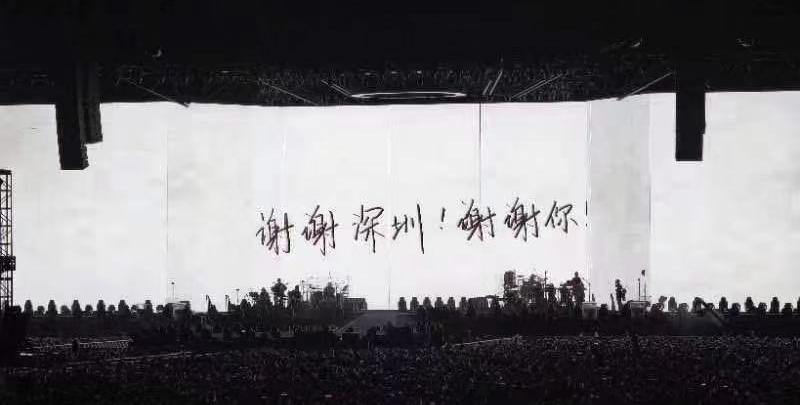
\includegraphics[width=400pt]{img/shenzhen20240601/thank-shenzhen} 

}

\caption{谢谢深圳!谢谢你!}\label{fig:unnamed-chunk-44}
\end{figure}

\hyperref[listen-to-me]{🎵【\textbf{听我说}】} 跟我一起好吗\textasciitilde?\textbf{谢谢你们总是愿意去听我说很多我的不开心,或者是很多我的心情,也希望你们不开心的时候也都多多跟我说},好吗?(米:好\textasciitilde)一起\textasciitilde{}

\hyperref[hope]{🎵【\textbf{望}】}无论你在哪里,只要你需要,我都在这里。全场\textasciitilde 交给你们\textasciitilde{}\textbf{我是真的,因为你们我不再孤单,我(深:心有所住),谢谢,谢谢。}

  在我最后一秒想要给大家隔空一个大拥抱的时候,我的一个扣子崩开了。等一下,为什么啊啊啊啊?谢谢你,大家平时会爱玩游戏吗?你们玩得厉害吗?哈哈哈,好多很诚实的人跟我一样玩的不厉害,但其实很多人都会说人生很多时候都像一场游戏,大家总会觉得输了怎么办,或者是玩游戏玩不好怎么办?不用害怕,输着输着就赢了对不对?因为我也在想,难道奇迹时刻只属于赢的那个人吗?但其实并不是,我们输着输着我们也会拥有我们的奇迹时刻,那个就是慢慢慢慢成长的我们,\textbf{所以不要害怕,所有的东西都会过去,我们去迎接我们的奇迹(米:时刻),没错。}

\hyperref[magic-moment]{🎵【\textbf{奇迹时刻}】}亲爱的观众朋友们,大家给我一声鼓励,321,加油,321。谢谢你们,\textbf{拥有你们就拥有奇迹时刻。}

\begin{figure}

{\centering 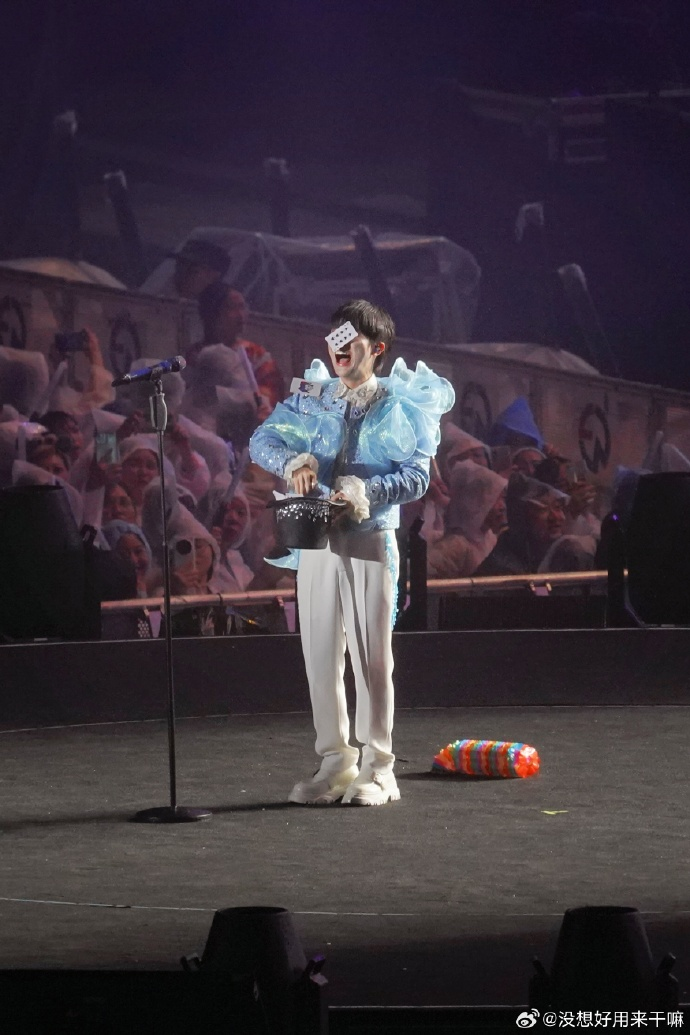
\includegraphics[width=400pt]{img/shenzhen20240601/001} 

}

\caption{深圳萌术师 【@weibo-7499】}\label{fig:unnamed-chunk-45}
\end{figure}

  谢谢大家,我是不是厉害的魔术师?(米:是),真诚一点好不好,以后做人,哈哈哈。哎,自己弄乱的舞台,自己也暂时收不干净。但是里面有个小小的小惊喜,\textbf{就是我变出了一个平字,希望大家永远平平安安。}耶,好啦,我觉得以后变魔术这个事儿真的有点难,但是刚才应该还可以吧?(米:可以),这边的朋友应该觉得也还可以吧?(米:可以)。刚才再精彩的魔术应该都不及我刚才跟这个彩带之间的一些争斗,哈哈哈,那我觉得一切我都非常开心。所以无论如何不要害怕输,我们总会赢的,我们总会收获我们的奇迹时刻,对吗?(米:对),没错,就像我打王者荣耀,我也不厉害,但是我也可以收获到很多开心和很多奇迹时刻。那这首歌接下来也是我非常喜欢的一首歌,它充满着力量,然后很多人会觉得听完他会觉得非常励志,而且特别适合最近听,马上就要到高考的时候,而且有很多要考试的同学,我们每一个人都是去追求梦想和追求更好的自己的璀璨冒险人。Wuuu,那你们会唱这首歌吗?(米:会),那等一下跟我一起唱哦,(米:好),\textbf{我们一定都会收获属于我们自己的璀璨的。}

\hyperref[adventurers]{🎵【\textbf{璀璨冒险人}】}你们会吗\textasciitilde?全场\textasciitilde(米:还想要继续吗)要(米:要逆风不退啊)(深、米:向心中的梦啊)我们(米:去追吧)

【\textbf{点歌环节}】谢谢我们的舞者们,谢谢大家,掌声给他们。从前也有很多人告诉我,说我在舞台上很容易被舞台吞掉,看不见,我也从来没有想过自己有一天会在体育场开演唱会,让我再听一下,好吗?你们好吗?(米:好),所以你们真的,\textbf{周深都可以做到,你一定也可以做到},好吗?(米:好),接下来是我们非常开心的点歌环节,在此之前\textbf{我今天也是儿童节的一个开心的小朋友,所以我想先让你们给我唱首歌},好吗?(米:好)有一首歌应该算是跟深圳非常有缘分。(深:灯火里的中国青春婀娜,灯火里的中国胸怀辽阔,灯火灿烂的中国梦,灯火荡漾着心中的歌。)怎么最后还是变成了我唱?哈哈哈。好,那接下来就是我们的摄像老师会随机抓取一位朋友,然后你将会在9首歌里面选一首你想听的歌。我相信很多生米们看完这些歌单应该很开心,因为它们相对来说比较冷门,所以希望抽到你,你能够听过这些歌,但也不要有压力。我们现在随机开始,我们全场倒数5个数,好不好?来喽,老师,可以随便找,找个远点都可以来。5(米:4321)。好,就是你,哈喽,你在哪里?哈哈哈,哦,在这儿吗?在这儿吗?哈喽,你好,是你吗?哈哈哈,(深:是你吗?)哎哎,我有找对啊,是你,是小朋友吗?hello,你好,怎么称呼你?加一波?再加一波歌单,可能不太行。哈哈哈,平时怎么称呼你小名?瑶瑶,好,欢迎瑶瑶小朋友,我们一起祝瑶瑶小朋友儿童节(米:快乐)。你几岁开始听我唱歌的呀?3岁?你现在几岁?9岁,你也是我的6年老歌迷了,哈哈。你,你是哪里的人?就深圳的吗?广州来的啊,哦,谢谢你,特别感动,因为你的飞机或者是你的高铁有延误吗?或者你是开车过来的还是怎么过来的?坐高铁过来的?对,因为我坐飞机过来的时候也延误,然后就很着急,\textbf{当然我觉得很开心,无论怎么样我跟大家见面了,你们好!}(米:好)。瑶瑶,小朋友,你知道你是i人还是e人吗?你是e人?来,舞台给你,哈哈哈,你随机选一首歌,你来唱,上面有你听过的歌吗?Oh,真的有吗?你想选哪一首?时结,因为时结这首歌就是写给很多咱们中国传统节日的歌曲。好,谢谢瑶瑶小朋友。谢谢你,好可爱。哇,谢谢。\textbf{作业做完了吗?}哈哈哈哈,谢谢瑶瑶,真的很应景,因为这首歌就是里面写了很多很多咱们传统的节日,然后刚好又在六一儿童节,大家,希望大家都能够每天都有个好的心情,都像过节一样,好吗?(米:好)时结。

\hyperref[shijie]{🎵【\textbf{时结}】}嗨起来,你点的歌,瑶瑶。好了好了,不要害怕我,不要害怕我。

\hyperref[keep-playing]{🎵【\textbf{不想睡}】}到你们\textasciitilde 这里有布丁吗?有生米吗\textasciitilde?这边\textasciitilde 全场\textasciitilde(米:lalalalalala\textasciitilde)全场最后一次(米:lalalala\textasciitilde)谢谢你们,谢谢大家\textasciitilde{}

  谢谢大家。谢谢每一个听过我的人,谢谢你们还记得我,谢谢你们。后面看台的朋友你们好吗?这边?我真的,在,就平时看一些演唱会的视频,就人家的歌手都是指哪里,哪里的尖叫声都特别大声,我想试一下这是不是真的好吗?那现在安静。(指哪哪尖叫游戏)谢谢谢谢谢谢谢谢谢谢,也谢谢每一位,哈哈哈,可能是开心的头晕,也谢谢每一位老师能够帮助我,让我被看见。所以我觉得自己非常非常幸福,我们一起来感谢一下让我们美好遇见的人们,好吗?(米:好)

  非常感谢深圳市公安局,感谢龙岗公安分局。wohu\textasciitilde{} 感谢龙岗区文化广电旅游体育局,感谢深圳市公安局交通警察局,感谢龙岗交警大队,感谢深圳市消防救援支队。感谢深圳市龙岗区消防救援大队,感谢深圳市公安局轨道交通分局。最热烈的掌声,再感谢一次,也非常感谢我们的场地支持深圳大运中心。感谢我们的本次巡演的全程主办,我们的老朋友北京时代立方文化传播有限公司。熟悉我的人就会非常熟悉他们,因为是当我还没有被那么多人看见的时候,在他们,就陈总他找我去做的第一次自己的个人巡回演唱会是C929-星球。所以我该怎么去形容,我不敢想象会有那么多人会愿意为了周深这两个字来到现场。我刚开始的时候是在live house,最多的人的live house,我记得也就是1000多,或者到后面可能会稍微大一点,但可是这里相当于做了40多个Live house的朋友们,谢谢你们,谢谢,也谢谢我们深圳站的承办上海魔方泛文化演艺有限公司,今天的演唱会你们喜欢吗?(米:喜欢)。谢谢你们。\textbf{\textcolor{red}{我也非常喜欢你们}},谢谢演唱会制作单位必应,谢谢我们的总导演周佑洋、庄惟惞。今天你们听我的声音好听吗?(米:好听)我唱歌好听吗?(米:好听)哈哈哈。真的要非常感谢我们的音响总监金少刚,我跟少爷,我们大家都称呼或者是怎么说?金老师,我们平时我的性格你们知道的,\textbf{我不太会去频繁的打扰别人,但是就会发现当你需要帮助的时候,你身边的老师或者是甚至是很久都没有联系人,他愿意来帮助你,是个非常幸福的事,你们要相信这样愿意帮助你的人也有,所以我们继续好好去追逐自己,好吗?(米:好)}谢谢金老师,也非常感谢我们的音乐总监龙隆老师,感谢我们今天的乐队老师们,感谢我们的和声老师们,感谢我们的舞蹈团的SDT ShowPro。我们每一次的相遇,真的,我们所有的幕后老师们其实心情跟我一样的,像我一样,迫切的希望跟大家见面,也都像我一样喜欢你们,谢谢你们。谢谢我们的服装团队设计师劳伦斯许工作室,以及时装品牌windowsen。谢谢我们的音响工程,南京奥斯泰视听科技有限公司,谢谢我们的调音团队,乐尔工作室,谢谢硬体工程北京力超舞台集团哦。谢谢周深工作室的小伙伴们(米:啊啊啊啊)。哈哈哈,你们,哇塞,你们,谢谢你们,哈哈哈,我们很意外,谢谢大家,谢谢大家,谢谢大家,谢谢你们,然后谢谢票务总代理大麦网(米:倒闭)。哎,哈哈哈,谢谢票务代理猫眼票星球(米:倒闭)。怎么回事?感谢微博,感谢微博音乐,感谢微博演出,呦吼。以及最重要的是感谢我们现场的所有工作人员们,谢谢他们。当然最重要的是要感谢每一位,应该是克服了很多困难,或者克服了很多纠结的事情,或者甚至是刚开始我们见面之前还带来了很多,就怎么说,心情还有很多不开心的那些心情,但是最终我们见面了的你,谢谢你,谢谢。

  如果非常熟悉卡布的就知道了,不想睡已经是最后一首歌了,不想睡是卡布的晚安曲,\textbf{那很幸福的是,嗯,周深有了一首自己的晚安曲,叫我以渺小爱你}。在演唱这首歌曲之前,我想跟大家拍个照片,好吗?(米:好)谢谢,我们场灯老师非常的棒,给大家开亮的场灯,可以看到,来,我们先中间拍一拍。好,咱们速度一点哈,来,这边的朋友,哦哈,我的膝盖湿了,哈哈哈,我会不会挡住?321。好,中间的朋友,中间一点啊,321,好,左边的朋友。321,我们迅速,两边,赶紧赶紧,赶时间呢,赶时间呢,这边这边,感觉自己录了一期跑男啊,321,那边那边,(深:我会奔向你,我会奔向你)开完一场演唱会,微信步数26000。哈喽,我看到明天他生日,祝你明天生日快乐。祝今天生日的你生日快乐。哇,原来体育场这么大,哈哈哈,体育课考试的时候也不过如此了吧。允许我喘一口气,不过真的非常感谢每一个到场的你,我以渺小爱你,希望你能够听到。

\hyperref[loving-you-in-my-humble-way]{🎵【\textbf{我以渺小爱你}】}我以渺小爱你,谢谢你没有嫌弃我,谢谢\textasciitilde 谢谢你们,\textbf{我也会继续加油的,更好的跟你们相遇,我们更好的见面,好吗?(米:好)。}

\section{Part5}\label{shenzhen-20240601-part5}

\hyperref[the-wind-rises]{🎵【\textbf{起风了}】}谢谢你们还在\textasciitilde 到你们\textasciitilde(深:逆着光行走,任风吹雨打)我们都不怕,对不对?(米:对\textasciitilde)这边\textasciitilde{}\textbf{(深:以爱之名,你还愿意吗?)(米:愿意)你还愿意吗?(米:愿意)}

\hyperref[big-fish]{🎵【\textbf{大鱼}】}

  谢谢大家,我觉得大鱼最后一句,倒流回最初的相遇的相遇两个字也特别像我们每次的相遇,真的很难相相xxi遇。就那些全场(深:倒流回最初的xuxixi相遇)。哈哈哈,我们来一遍最整齐的,(深:倒流回最初的)(米:相遇)谢谢你们。以前我的演唱会都通常,以就是大家泪流满面结尾,所以\textbf{这一次9.29Hz,我觉得我要跟我,能够愿意跟我同频的人,愿意跟我同频的你,我们无论如何都要开开心心的结尾,随时都可以想到这个时刻都是最美好、最快乐的回忆,所以这一次的最后一首歌是少管我。}很多不太清楚这三个字的人,我要稍微解释一下,这是我跟生米,或者是跟歌迷之间的一个小小的一个,一个就是一个默契,或者是一个玩笑,就一开始就反正就反正是,啊,少管我。但它其实,怎么说呢,是想说的是所有的事情它并不是对,或者是错,或者所有的事情也不像是少管我这三个字初听起来感觉像是充满棱角或者是比较凶的一个态度,而且很多时候我觉得更是一种理解,因为很多时候一些带着爱的一些建议或者是要求,很多时候我们也可以摘取去听。但更多的是我们还是要去选取自己最清楚的那个方向去向前进,但中途我们不一定要去争论或者是不开心,所以这首歌的风格是非常轻松活泼的一首歌,也希望这首歌可以随时喊zhou你们,喊走,也希望这首歌可以随时喊走你们所有的不开心,好吗?(米:好)

  然后现在到了我最喜欢的一个环节,就是少管我Camera,哈哈,这句英语说的特别不像英语,少管我相机,就是当我们的摄像老师拍到谁的时候,你就要用我们比较有趣的这个姿势。嘿,少管我,来把你所有的不开心喊走,好吗?(米:好)好了,来喽,全场倒数五个字,五个数字5,(米:4321)。好,又是我们的小,hello,你好,是你吗?哈哈,怎么感觉有点眼熟,哎哎,在哪里?是在这里吗?哈喽,您好,您是从哪来的?不会是从广东吧。没事,我们两位一起,您是从哪来的?跟瑶瑶一起的哈,我们都熟都认识啊,后面这位朋友你是哪里的?对,你也是广州来的哦,你们是一起来的吗?哈哈,不是,哈哈哈,好,谢谢你们,谢谢你们。那你们能有学好这个姿势吗?然后我们来两个人同时双方一起,对,你们俩,交个朋友们嘛,来321,还有个嘿,哈哈哈,来全场我们先预演一遍321,(米:嘿,少管我!)对对对,来喽,321,嘿,少管我!没错,\textbf{希望这一声可以喊走你所有都不开心好吗?}要开开心心的回广州,哈哈哈,谢谢你们。

  那么再来找一位朋友,在全场五个数(米:543)21。哈喽,小朋友你好,怎么称呼你?什么?丁羽西?魏雨欣?哈哈,看旁边有个大哥哥,看不下去了,``万羽西''。所以叫什么?小名怎么称呼你?西西,早说就好了嘛,哈哈哈,西西小朋友。你也有什么不开心的时刻需要喊少管我吗?哈哈哈,也有啊?哦,没有,那你坐下。哈哈哈,不会不会,西西小朋友,我们来一次,就是这个不是告诉你所有的东西要去吵架或者怎么样,而是所有的东西大家都可以有一个温柔的角度去解决,好不好?你做少管我的时候记得不要打到前面那位朋友的头,哈哈哈,来321,西西小朋友。哈哈哈,非常棒,那我们全场再来一遍。321。嘿,少管我,希望你们喜欢,哦吼。

\hyperref[watch-ur-manners]{🎵【\textbf{少管我}】}全场\textasciitilde 全场(米:嘿,少管我)非常棒,再来一次,54321,(米:嘿,少管我!)全场\textasciitilde 来,嘿(米:少管我!)谢谢大家的到来,一定要注意安全,平平安安回去,东西不要掉喽。谢谢你们,\textbf{所有的不开心都要随时想起我们今天制造的最快乐的回忆,把不开心全部赶过去,好吗?}(米:好)谢谢你们,看台的朋友,后面的朋友,谢谢,谢谢大家。再来321(米:嘿,少管我),谢谢你们,太棒啦,wuhooo,谢谢,看台的朋友,谢谢大家。321,走(米:嘿,少管我!)谢谢你们,谢谢,54321,(米:嘿,少管我)\textbf{你们太棒了,谢谢你们,你们是最棒的观众,你们也是最好的那个人,好好照顾好自己好吗?(米:好})大家要注意安全,东西不要掉喽,谢谢你们愿意跟我同频,也希望你们平平安安,天天开心,照顾好自己,拜拜!

\begin{center}\rule{0.5\linewidth}{0.5pt}\end{center}

\begin{figure}

{\centering 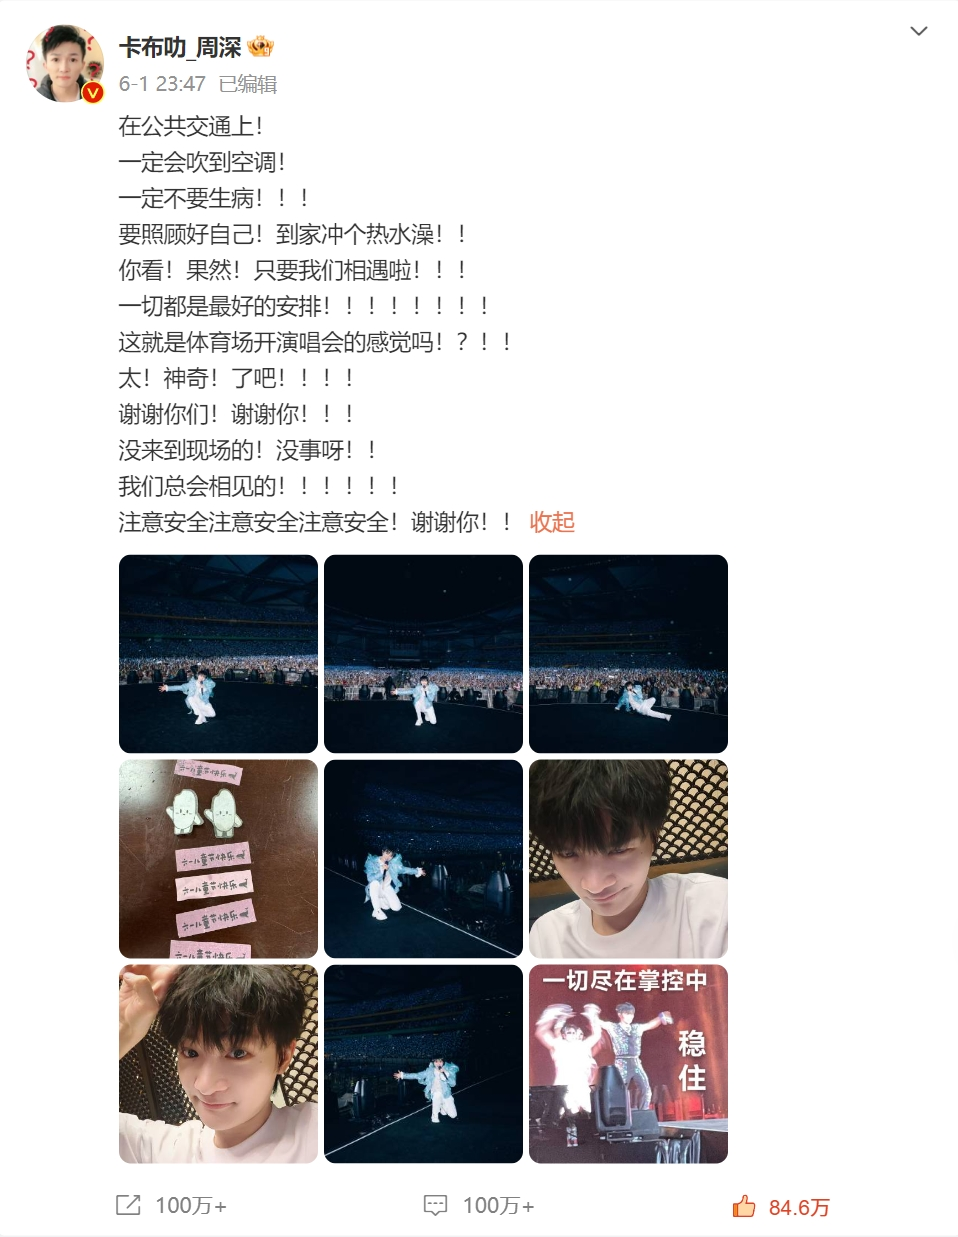
\includegraphics[width=400pt]{img/weibo/shenzhen-20240601} 

}

\caption{周深深圳大运中心体育场演唱会结束微博 【@weibo-charlie】}\label{fig:unnamed-chunk-46}
\end{figure}

\chapter{2024.06.15成都场}\label{chengdu-20240615}

\begin{quote}
\textbf{\emph{只要你需要我,无论你在哪里,我都在这。------ 周深}}
\end{quote}

\begin{figure}

{\centering 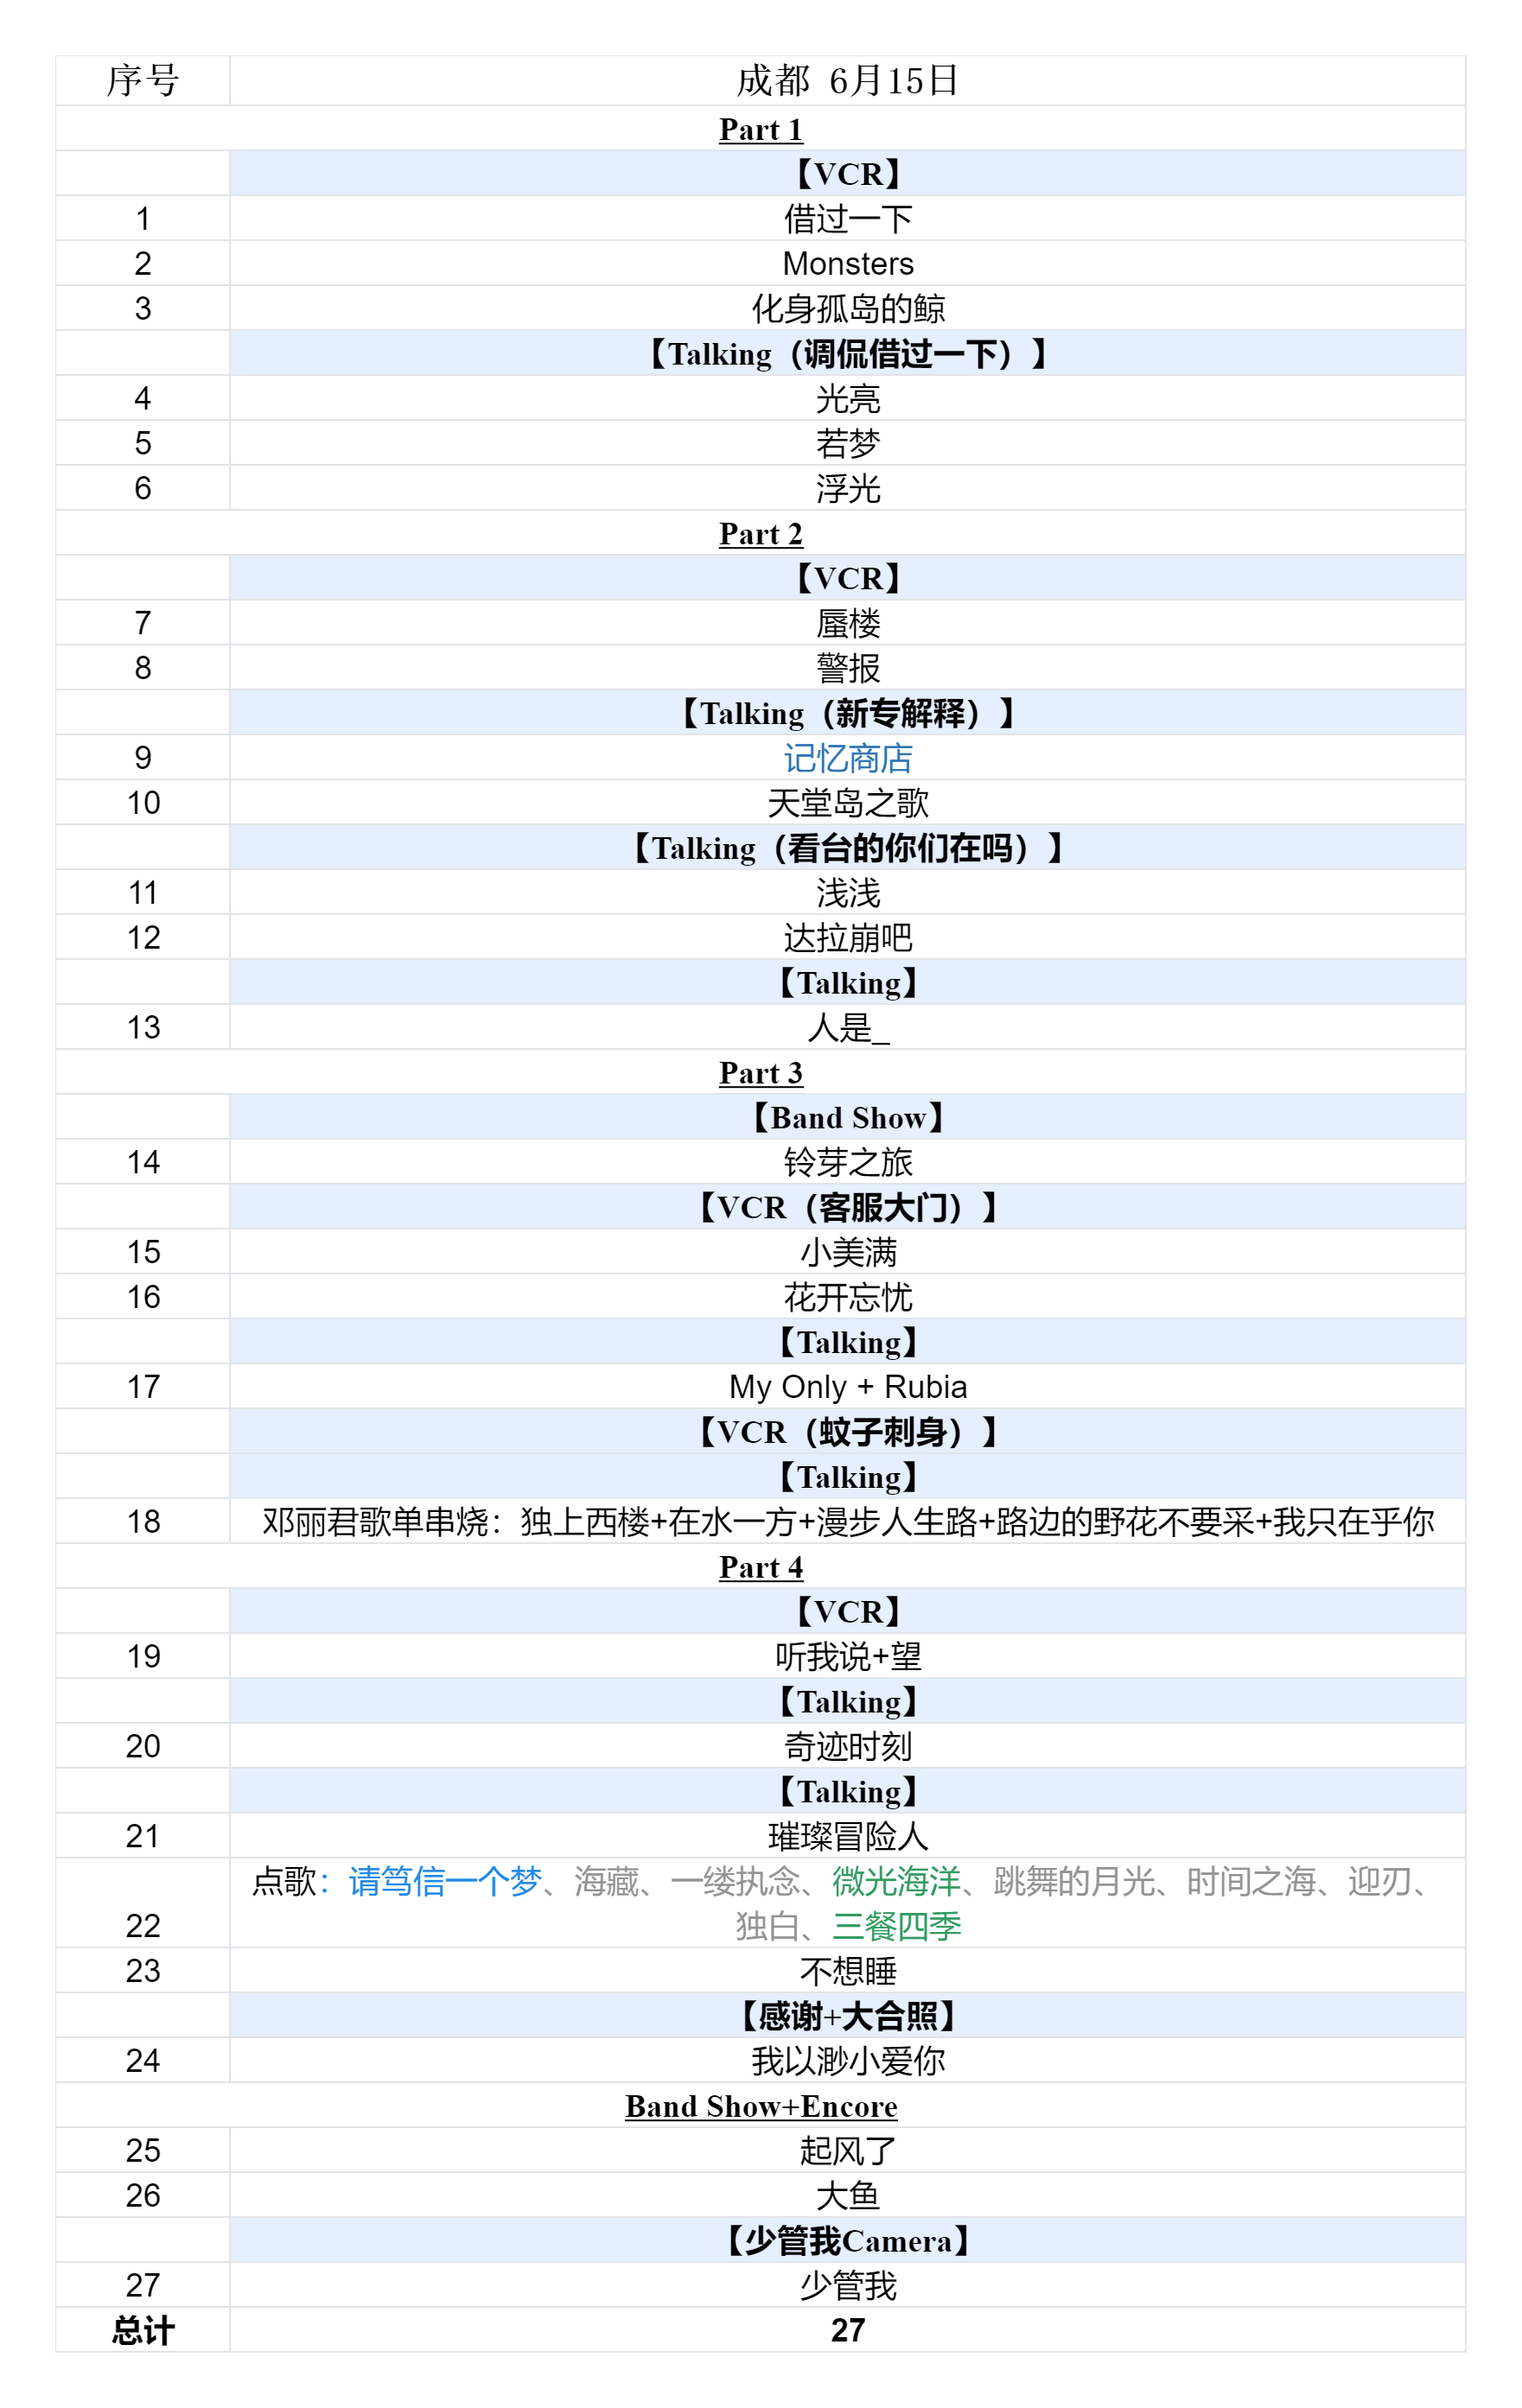
\includegraphics[width=300pt]{img/playlists/playlists-chengdu-20240615} 

}

\caption{2024周深9.29Hz巡回演唱会2024.06.15成都场歌单}\label{fig:unnamed-chunk-49}
\end{figure}

\newpage

\section{Part1}\label{chengdu-20240615-part1}

\hyperref[opening-vcr]{🎥【\textbf{开场VCR}】}

\hyperref[I-will-go-my-way]{🎵【\textbf{借过一下}】}成都的朋友们,你们好吗?

\hyperref[Monsters]{🎵【\textbf{Monsters}】}

\hyperref[hua-shen-gu-dao-de-jing]{🎵【\textbf{化身孤岛的鲸}】}你们会唱吗\textasciitilde 大声点\textasciitilde 再来\textasciitilde 到你们\textasciitilde(米:没有墙头)这句专门为了我们成都场,(\textbf{深:无论你迟到多久,也依旧是我心中的王后})谢谢\textasciitilde{}

  成都的朋友们,你们好吗?(米:好)大家好,好开心好开心,也是从来没有想过会看到那么多人,在(唱)《借过一下》,真的在借过一下 。可能因为外面是不是稍微有点堵车?是,所以看到稍微有些朋友们稍微有点迟到,就我在台上,\emph{让我大醉一场},他们在,诶,不好意思,借过一下,不好意思,他们在找自己的位置。我就觉得特别特别开心,因为好开心没有下雨诶。我其实也有想过,因为其实今天的温度也没有算非常热,对不对?所以我准备的一个,怎么说呢,一个梗吧,就想的是如果今天非常热的话,那我们今天都可以到四五成熟,我们都比较是熟人了,结果,哎呀,心情很畅快,因为天气还不错,所以成都的朋友们你们好吗?谢谢你们,我想说我们人生当中的相遇就是这样的,我们没有办法去规定哪个时间点,我们一定要相遇。但是有的人说,哎呀,有的人会知道我是布丁吗?就很多生米,他们就会说好像我认识周深,认识迟了,或者甚至是有点点迟到了。但我觉得无所谓,\textbf{只要你来我就已经非常荣幸了},谢谢你们,后面看台的朋友,你们好吗?\textbf{我觉得我在自己奋斗的路上永远是一个人在漆黑的隧道中去行走,但是我觉得自己非常幸福和非常非常幸运,因为有你们愿意去照亮我前行的路,你们总说我是你们的光亮,但是其实你们才真的是我的光亮。}谢谢你们,谢谢你们出现在我生命当中,谢谢你们。那这首光亮希望也可以照亮你,每次感到孤单的时候,光亮希望你喜欢。

\hyperref[silver-linings]{🎵【\textbf{光亮}】}还有朋友在借过一下,注意安全\textasciitilde 谢谢大家\textasciitilde{}

\hyperref[ruomeng]{🎵【\textbf{若梦}】}接下来这首歌你要帮我一起唱哦,对,因为\textbf{每次想到这样的场景,每次一想到遇见大家,都像做梦一样。}(\textbf{\textcolor{blue}{米:妈妈爱你} })爱你个头啊\textasciitilde(深:往事流转,在你眼眸)你们(米:一边遗忘一边拼凑)这边\textasciitilde 你们唱的真的非常非常好听\textasciitilde 后边的朋友们\textasciitilde 看台大声点\textasciitilde 这边的朋友,到你们了\textasciitilde(深:因为你们,我才得到拯救\textasciitilde)

\hyperref[floating-light]{🎵【\textbf{浮光}】}(米:宝贝)我现在可高冷了,我什么都不回答\textasciitilde{}\textbf{谢谢这人间恍惚三万天遇见了你,谢谢\textasciitilde{}}

\section{Part2}\label{chengdu-20240615-part2}

\hyperref[senself-vcr]{🎥【\textbf{反深代词VCR}】}

\hyperref[mirage]{🎵【\textbf{蜃楼}】}

\hyperref[the-giver]{🎵【\textbf{警报}】}你们会唱这首歌吗?(米:会)要记得保护好自己\textasciitilde{}

  谢谢,谢谢大家,刚才的歌你们喜欢听吗?(米:喜欢)谢谢你们这么给面子。哈哈哈,因为刚才两首歌是我的全新专辑(米:反深代词),对,反深代词的两首歌。前面第一部分那些歌是大家可能比较熟悉,然后古风抒情的,一个比较以前的我吧,然后我觉得反深代词当中他是一个全新的我,但是为什么会出现这样一个全新的我?这就要谢谢在场的每一位,或者是没有在现场的每一位给我那样的勇气和力量去寻找自己。\textbf{反深代词当中每一首歌其实都有很多自己想说的话,就比如像蜃楼,他说的其实是,很多人可能被执念困住,停在原地没有办法动,也可能有一些好的执念会去帮助你成为更好的自己。那警报呢,就写的是身边很多很多非常善良的人,他们可能照顾好了全世界,但是唯独忘记去照顾好自己。}其实我觉得也很像我自己,我一开始的时候我有那种执念,就是我要告诉大家我唱歌唱得还不错,我可以唱高音,啊啊啊啊啊,我还可以变换声音,比如像这个样子给大家唱歌,其实就是这样一个执念,让我不停地去,想要证明自己,说实话,有点累,哈哈哈。然后警报也会像我以前的性格,以前会觉得我想照顾好所有人的情绪,或者是我想在意好每一个人在现场的一个状况。那后面发现好像经常忘记照顾好自己,所以这首歌或是整张专辑都是送给你,希望你们可以在里面找到一些你的碎片。我们要美好,也要善良,但是我们的善良也要长出牙齿。\textbf{对,然后和你的每一次相遇,我都是一起在制造一个非常美好的回忆。}如果200年以后有一个记忆商店。不知情的朋友们,我给你们解释一下,记忆商店是反深代词里面那首歌,\textbf{那如果在200年以后,我一定会立马冲进记忆商店去买这一份最甜、最治愈、最美好、最珍贵关于你的记忆,谢谢你们。}

\hyperref[the-memory-store]{🎵【\textbf{记忆商店}】}

\hyperref[haven-song]{🎵【\textbf{天堂岛之歌}】}

  \textbf{谢谢大家,有被你们的爱拯救了,我逃出去啦},非常非常非常,非常非常开心。然后我们这次演唱会的主题叫9.29Hz,因为自己从来没有想过自己会被那么多人听到,会有那么多人愿意去跟我同频,无论是以前大家比较熟悉的我,或者是像新专辑,或者甚至像刚才天堂岛之歌这样子比较新的我,所以谢谢你们愿意跟我同频,让我觉得自己不孤单。那,好像我没有听到我们看台朋友们的声音,你们在吗?这边的呢?确定不是那个荧光棒摆在原地吗?晃一晃我看一下。成都的朋友们,成都的朋友们(方言),你们好。很多人会,我有非常多的一些外号,就包括有很多比较陌生的人,就是不太熟悉我的人,然后他们会看见我的微博叫卡布叻-周深,他们一直以为卡布叻是个男团。哈哈哈,就感觉好像有周深、周浅、周果子、周可可,还有什么,周星星,等等等等,然后渐渐地开始习惯大家叫我一个名字,叫深深。我从来没有想过自己会接受这个外号,因为我觉得有丢丢的肉麻(方言),但是特别巧的是在我的第一张(专辑)。。。(米:宝贝)好,停,我不承认我有这样一个外号,我只能说,宝你个头乘以3.5万。解释一下宝你个头,就是我跟生米之间的一个互动。然后这首歌在专辑里面叫《浅浅》。

\hyperref[qianqian]{🎵【\textbf{浅浅}】}收回天气不热的对话,我一直在流汗,从今天开始,我们大家都熟了,不想和不熟的人说话,这个梗用上了。

\begin{figure}

{\centering 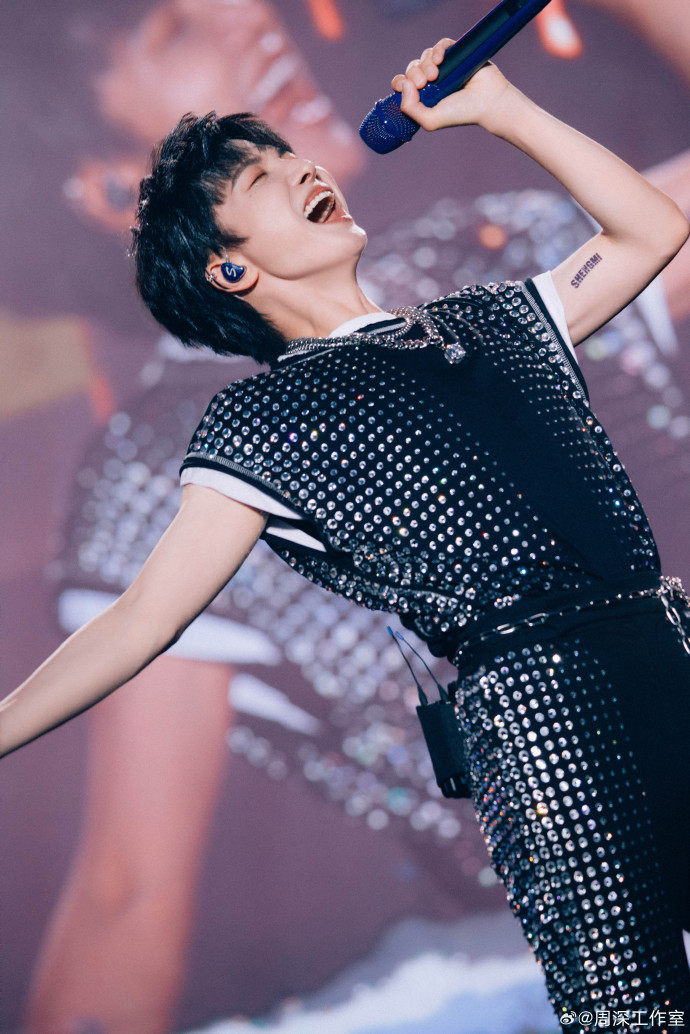
\includegraphics[width=400pt]{img/chengdu20240615/004} 

}

\caption{啊啊啊啊啊~ 【@weibo-charlie-studio】}\label{fig:unnamed-chunk-50}
\end{figure}

  好了,接下来不要光顾着啊啊啊了,因为接下来这首歌我要靠你们来唱。这首歌它是一个happy ending的童话故事,但是,我好像有点忘记了,没错,我是在装,哈哈哈。到底是谁打败了谁?谁又咬了谁?又救出了谁?最后谁和谁欢快地生活在了一起?有个孩子叫?(米:王浩然)你记性挺好,王浩然,那前面的谁和谁和谁和谁和谁?那他们到底都是谁呢?

\hyperref[dalabengba]{🎵【\textbf{达拉崩吧}】}现在轮到你们来复述这个童话故事了,到底是谁打败了谁,又咬了谁,谁又嫁给了谁,谁最后生下一个叫王浩然呢?来喽,这边,于是\textasciitilde 砍向\textasciitilde 咬了\textasciitilde 最后\textasciitilde 谢谢\textasciitilde{}

  你们太棒了,谢谢大家,没想到大家唱得这么好。那接下来这首歌,昨天楠哥有在歌手上演唱。说实话我非常的震惊和非常的感谢,因为楠哥,\textbf{孙楠老师是我从小听到大的歌手,而且在我心中是一个非常非常尊重的前辈},但是没有想到有一天能够跟楠哥一起录一档音乐综艺,更没有想到的是楠哥会在一个舞台上演唱自己的作品,我觉得被自己非常尊敬,然后非常喜欢的位歌手翻唱自己的作品是我的荣幸,所以非常非常感谢楠哥。然后还有更加让我感动的一个瞬间,就是楠哥他唱完之后给我发微信,他就说,深深,那首歌非常好听,然后甚至楠哥这样的前辈会觉得自己有一些部分,可能像,自己没有发挥的那么的出色,或者是跟自己想象中的处理不太一样。但是我在震惊的是像这样一位非常前辈的老师,还在不停地去追求自己更好的那个自己,我相信这个应该是楠哥的一个执念,然后才让他在大家每次面前一亮嗓的时候,大家都觉得,哇,不愧是孙楠,所以\textbf{再次非常非常感谢楠哥让这首歌被大家听到,让这首歌被更多的人听到},然后今天我在这里希望大家能够喜欢这首歌,人是,我们都是最棒的,不怕任何的困难,忠于自己的选择,对吗?(米:对)

\hyperref[renshi]{🎵【\textbf{人是\_}】}(深:孩童的双眸)你们好吗\textasciitilde 谢谢大家\textasciitilde 你们愿意与我携手走过吗?(米:愿意)你们好吗\textasciitilde{}

\section{Part3}\label{chengdu-20240615-part3}

\hyperref[travel-lingya]{🎵【\textbf{铃芽之旅}】}大家听过这首歌吗?(米:听过)

\hyperref[close-door-vcr]{🎥【\textbf{关闭客服大门VCR}】}

\hyperref[happy-ending]{🎵【\textbf{小美满}】}这首歌你们会唱吗?(米:会)要用最大的声音唱哦?大声点\textasciitilde 太棒啦\textasciitilde{}\textbf{你们唱的太好听啦,比原唱好听多了},这边\textasciitilde 大声点\textasciitilde 大家好,我是周深,你们好吗?小美满这首歌,每次一听我会觉得非常非常的幸福,我也相信听到这首歌的人,所有的美好都会冲向你,所以我觉得这首歌很适合许愿,就像我现在这样子,默默许下一个愿望,321,我的愿望就可以挂在这颗许愿树上,那现在,无论你是什么工作,无论你年纪多大,我都希望你可以默默地一起许下一个愿望,那现在,每个人都闭上眼睛,默默地许下这个愿望,想一想你最想对自己,最想祝福的,但是在这里许的愿望有一个要求,大家要听话啊,这个愿望只能关于自己,想想最近有没有好好照顾自己啊,有没有像小美满一样让自己好好爱自己,许好了吗,321\textasciitilde 谢谢你们让我拥有很多很多很多的小美满,你们的愿望我们都会听到的。

  大家有看到这上面,哎哎哎哎哎哎哎,哈哈,有四棵许愿树,有第一站上海的两棵,然后是深圳的一棵,以及我们今天一起许下愿望的这一棵,大家有感受到满满的爱意吗?(米:有)然后在深圳的时候,大家记不记得就是大雨落下,浪费了我所有的妆发,甚至在说这段话,我还单压。那天有一个非常非常小美满的时刻,就是我在深圳的时候,我说自己就是下雨天的时候,可能自己的一些小故事吧,就是爸爸妈妈从来没有来接过我。然后突然回到家我就看到自己微信,就是小美满的这个词作李聪,他的妈妈就给他发了一个微信,他说他刚才在那个社交媒体上看到了我说的这段故事,他就给李聪应该算是有一半的道歉在里面。他说以前你经常说过这个事儿,好像我心中没有当过一回事儿,也许当时的你真的是不开心了吧?然后那一下我就觉得好温暖,然后李聪跟我说了最后一句话,就是我心中的那一小块好像一下子都长好了,然后我听到这样的回复之后,我自己心中缺失的那一块,也一下就全部变好,我觉得这样的小美满都是你们送给我们的,也希望在,\textbf{也许在无论任何时候你都觉得自己在淋雨,但是都要勇敢的相信真心和真爱。也许你现在还在淋雨,但是请勇敢相信那个爱你的那一把伞,他可能会迟到,但是他一定会到,但是所有都要基于你好好照顾好你自己。}花开忘忧,愿你无忧。

\begin{figure}

{\centering 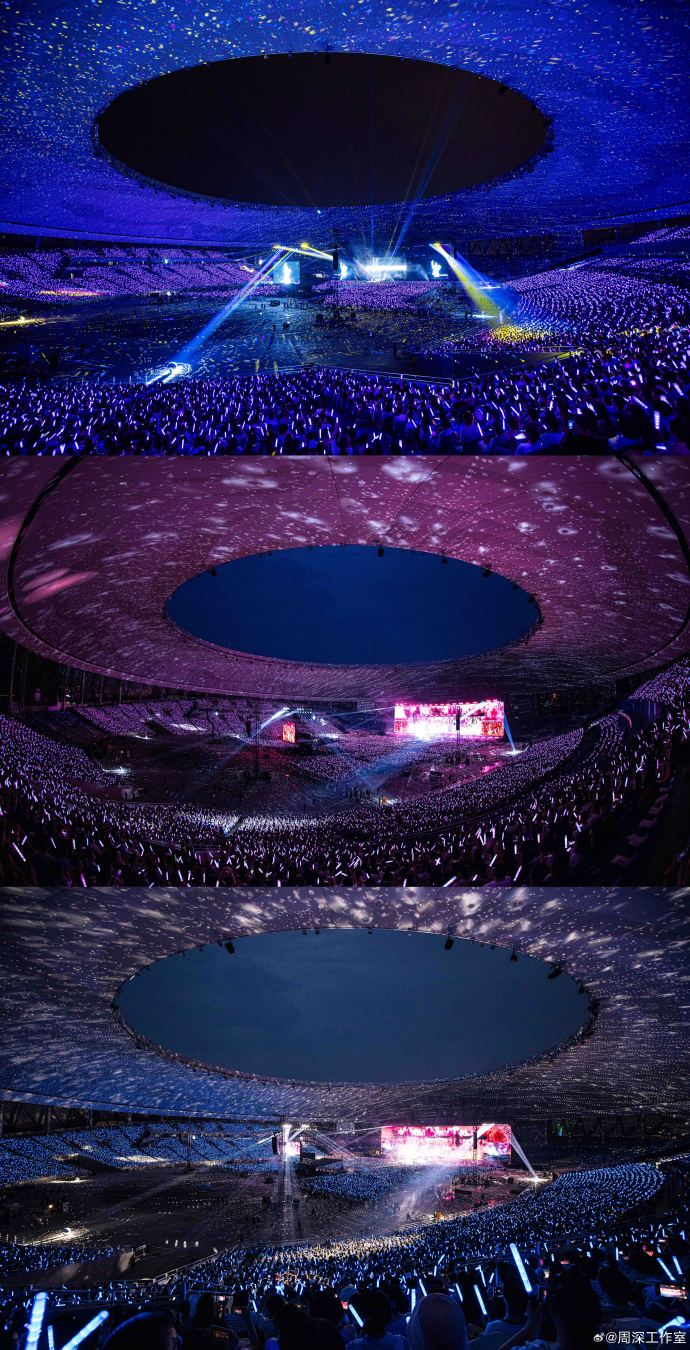
\includegraphics[width=400pt]{img/chengdu20240615/003} 

}

\caption{星空顶 【@weibo-charlie-studio】}\label{fig:unnamed-chunk-51}
\end{figure}

\hyperref[no-worries]{🎵【\textbf{花开忘忧}】}(深:我会说)(米:你好啊)(米:别走远了一起回家)一起回家好吗\textasciitilde 到你们\textasciitilde 我们的思念一定会被听见,对吗?(米:对)谢谢大家\textasciitilde{}

  大家有看到我们舞台中间,(米:宝贝)宝你个头,舞台中心放着一个非常非常漂亮的,琴。(米:哇哦\textasciitilde)不要哦了,这么漂亮的钢琴下面装了一个破碎的我,哈哈哈。但是我很喜欢这两首歌,我觉得他每次听起来就会有一种非常美好,非常的浪漫,然后感觉一切哪怕是不完美都会成为生命当中的小点缀。希望你们能够喜欢,也非常感谢你们,无论在任何时候或者任何地方,都愿意拾起那一片不完美的我的碎片。谢谢你们。没卡进去,刚才我那个披风掉的是谁笑得那么大声?大家装作没有看见好吗?我很成功很顺利的关上了那个门,听到不得哟(成都话),我好凶啊,哈哈哈。

\hyperref[my-only]{🎵【\textbf{My Only}】} \hyperref[rubia]{🎵【\textbf{Rubia}】}\textbf{希望我可以把所有的美好都唱给你们,你接受到了吗?}

  谢谢大家,刚才那两首歌你们喜欢吗?(米:喜欢)人人都知道,四川或者是成都的吃得非常好吃,我在这里帮你们光明正大的欢迎,哈哈哈。但是就在昨天彩排的时候,我有吃到一样东西,很多外地人一定都没吃过,甚至是本地人都几乎应该也没有人吃过的一个非常好吃的成都小吃,你们猜下是什么?不是,我们来请看VCR。彩排的时候就是,(播放VCR)。我居然在成都吃了蚊子刺身,哈哈哈,说实话他是有点辣哟(成都话)。然后你们知道吗,那个蚊子他没有``死'',他没有去世,他就在我的喉咙里边,一直在挣扎,救命啊,我要出去。我突然想到了西游记,就是``嫂嫂嫂嫂,我在你的肚子里'',然后我的嗓子眼非常的痒,非常的难受。作为一个歌手,你都在我的喉咙里,我还能拿你没有办法吗?我就一直唱高音,Life blooms like a flower,不出意外那个蚊子应该在我唱高音的时候被我的肌肉夹死在了,很神奇吧?我建议大家还是不要去尝试这样的刺身,有点刺挠,谢谢大家。

  那接下来这些,这一个串烧一个组曲,是应该算是我的音乐的启蒙者,我第一次听到唱歌就是听到她的声音,然后因为我有听到很多时朋友们也在现场,他们也会说那句,他说,深深哥哥,我们是从小听你的歌长大的。我记得在上海,在深圳场,你也是从小听我的歌长大的,谢谢你,我年纪也还可以,然后觉得自己很幸福,可以成为很多人听到歌声的第一位歌手。那她也是我听到歌声的第一位歌手,她就是我非常喜欢,应该说是对我音乐影响非常大的,邓丽君女士。这个组曲如果你会唱的话,请你跟我一起唱,好吗?(米:好)

🎵【\textbf{邓丽君组曲}】
\hyperref[one-in-the-building]{🎵【\textbf{独上西楼}】}来来来,想点什么歌,让我听到\textasciitilde 到你们\textasciitilde{}
\hyperref[on-the-water-side]{🎵【\textbf{在水一方}】}
\hyperref[walk-the-road-of-life]{🎵【\textbf{漫步人生路}】}这首你们会唱吗?全场\textasciitilde 嗨起来,刚刚你们唱的声音我感觉没有3.5万人哦,唱大点声音好吗?
\hyperref[only-with-me]{🎵【\textbf{路边的野花不要采}】}(深:路边的野花)怎么样?(米:你不要采)一起\textasciitilde 这边\textasciitilde 你们会忘记我吗?
\hyperref[only-you]{🎵【\textbf{我只在乎你}】}大声点\textasciitilde 谢谢你们,我也希望自己能够成为像邓丽君女士一样陪伴大家很久很久的歌手,记住我好吗?(米:好)

\section{Part4}\label{chengdu-20240615-part4}

\hyperref[thank-you-vcr]{🎥【\textbf{谢谢成都,谢谢你VCR}】}

\begin{figure}

{\centering 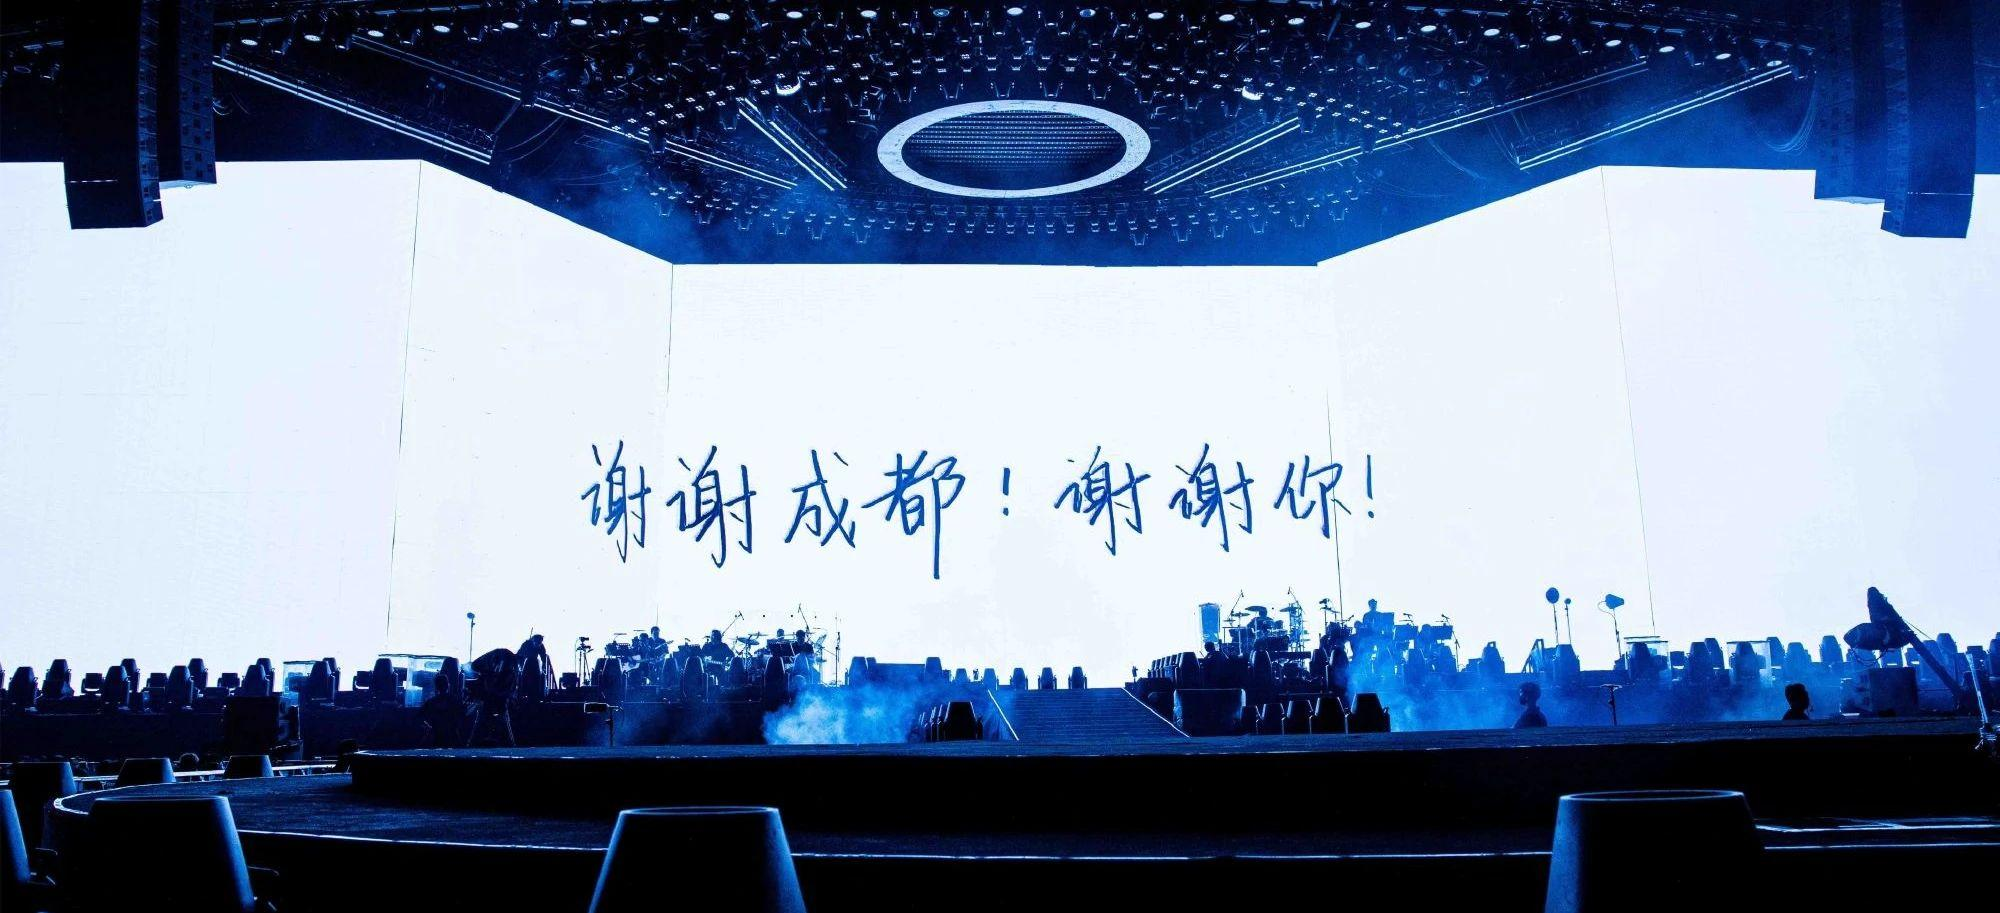
\includegraphics[width=400pt]{img/chengdu20240615/thank-chengdu} 

}

\caption{谢谢成都!谢谢你!}\label{fig:unnamed-chunk-52}
\end{figure}

\hyperref[listen-to-me]{🎵【\textbf{听我说}】}谢谢成都,谢谢你\textasciitilde 跟我一起好吗(米、深:听我说,可以听我说)(深:日子总会变好的)因为有你,日子一定会变好的\textasciitilde{}

\hyperref[hope]{🎵【\textbf{望}】}大声点哦\textasciitilde 因为你们(深:我心有所住,我不怕孤独)

  \textbf{所以无论你是在家乡打拼,还是在其他城市打拼,当你需要去表达一些事情的时候,不要害怕,就是要相信真心和真情,要大胆的说出来,只要你需要我,无论你在哪里,我都在这。}

  大家平时会玩游戏吗?打得好不好?你说打得好?你什么段位?你是王者?大家可能没有看到这位非常漂亮女士的表情,她说我是王者,没事,我打的不好,但是我是王者荣耀代言人。开玩笑的,开玩笑,我是觉得就是大家玩游戏不要老是害怕,或者我们人生其实也会就像一场游戏,每个人都觉得奇迹时刻只属于赢家,但是其实我也在思考,那我们这些可能打的不是很好的,所谓的打引号的``输家''会不会有奇迹时刻呢?会不会发现会输着输着输着我们就赢了,而且我们每一次出现在战场,或者出现在我们人生的那个考场的时候,我们都是那个赢家。而且非常巧的是,我一巡、二巡和这一次三巡来到成都的时候一直都在考四六级,今天也是在考四六级,现场有没有刚考完的朋友啊?(米:有)真的有吗?你最好说实话,哈哈哈哈,好的,\textbf{无论怎么样,不要让自己去失望,不要害怕前行,我们一定会收获我们自己的奇迹时刻。}

\hyperref[magic-moment]{🎵【\textbf{奇迹时刻}】}ladies and gentleman,这是一张粉色的丝巾和爱你们的红心,我需要大家的帮助,帮我一起吹一口好吗?321,哇,好大一股风啊,你们的爱心就会被吹进丝巾里面。还有哦,我好忙啊,救命,空的手心\textasciitilde{}

\begin{figure}

{\centering 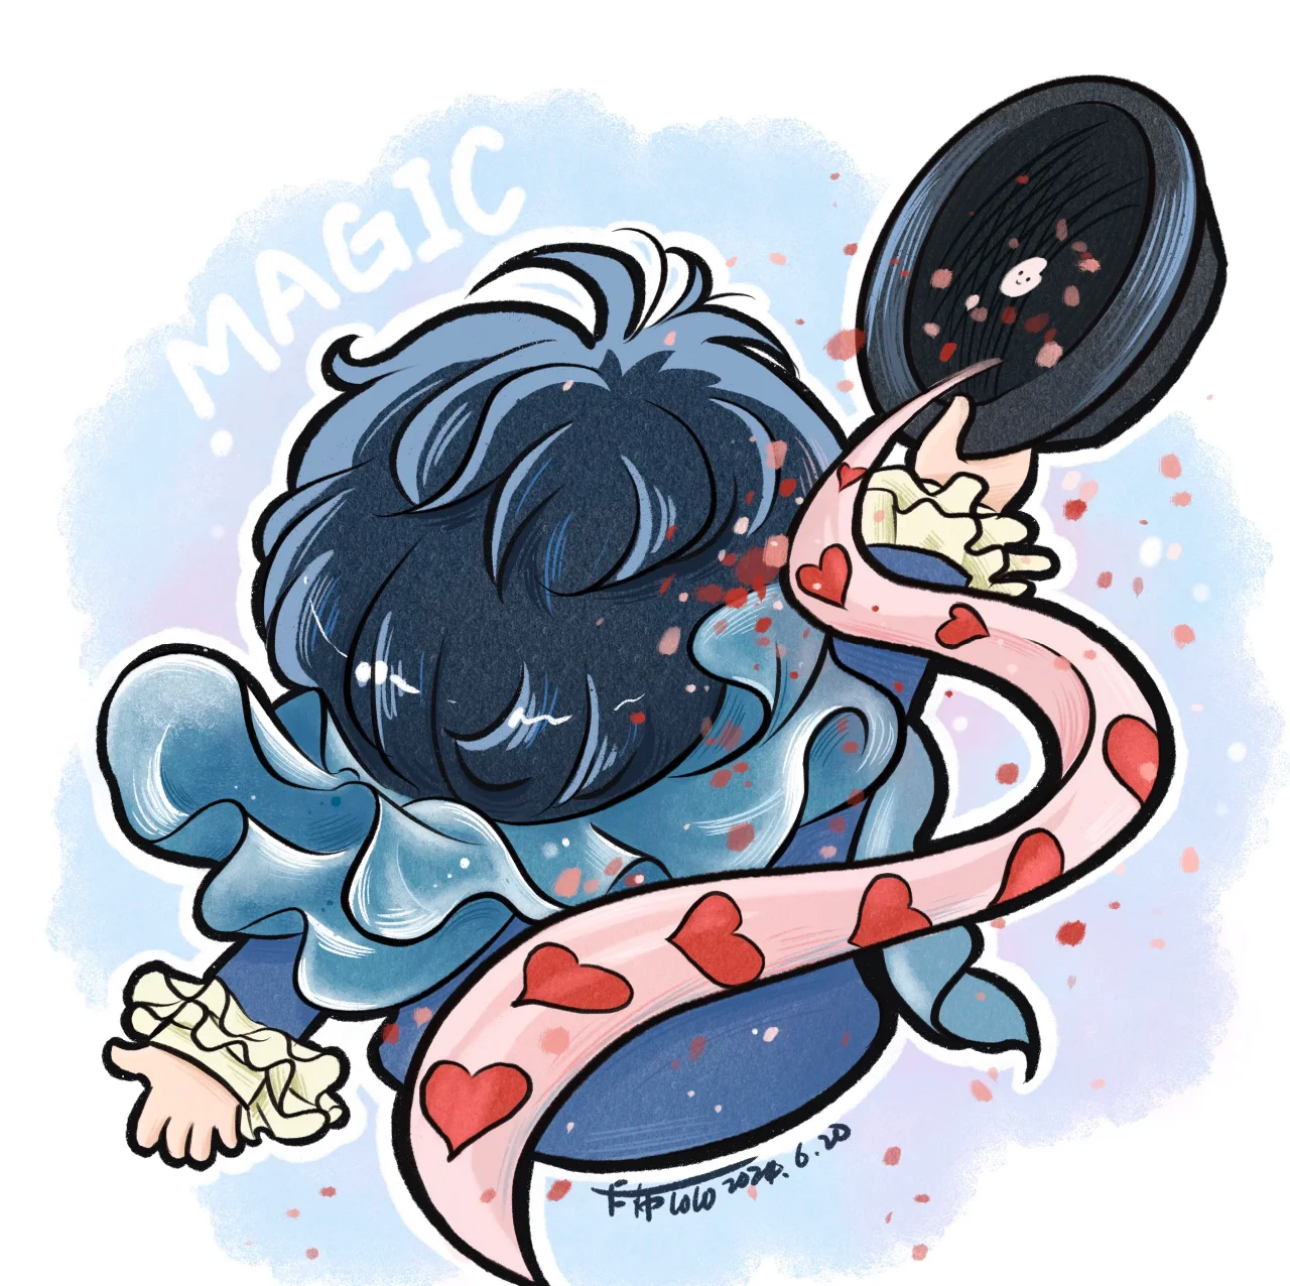
\includegraphics[width=440pt]{img/chengdu20240615/001} 

}

\caption{成都萌术师 【@weibo-charlie-studio】}\label{fig:unnamed-chunk-53}
\end{figure}

  我的魔术变得还可以吗?摇手是什么意思?变得还不错,是不是?我刚才在上面换衣服的时候,我的工作人员就跟我说,\textbf{当我唱第一首歌的时候,就有看见很多看台的朋友就已经是泪流满面。我当时听到心情特别的激动,我就会觉得,可能很多人会觉得一首歌有什么好哭的,但那一下我就明白,因为我们一起经历了非常非常多的事情。}

  我第一次在公开场合演出的时候应该是在路边,然后可能只有停在那里的十个人在听我唱歌。那10个人就是生米,就是歌迷,然后慢慢的会到了一些比较大的舞台,可能下面会有20个人,或者说50个人,但在后面可以有机会去 live house 开这个演唱会。开始到了1000多人,2000多人,就突然发现\textbf{今天大家见面真的是一个很治愈的奇迹时刻,他是对于我来说是一个非常珍贵的饼干时刻,因为每次在我自己沮丧或者说无助的时候,我都会去想起那个记忆,它可以治愈我很多,所以希望你们也好好的珍藏这份记忆,我珍藏这一份我们一起创造的记忆,在你需要的时候都来支援你},好吗?请你们相信你们非常非常努力,因为你们把一个这么普通的我,也慢慢的被大家看到,被大家听到。我站在这里就是你们创造的奇迹时刻,也希望我们每一个在追逐自己梦想的冒险人,你们一定可以收获属于你们自己的璀璨。这首璀璨冒险人跟我一起唱好吗?周深可以做到,你一定也可以做到的。大家可不可以做到我的衣服不用拖出来?

\hyperref[adventurers]{🎵【\textbf{璀璨冒险人}】}我们一起\textasciitilde 跟我一起好吗\textasciitilde(米:还想要继续吗)要(米:要逆风不退啊)冲\textasciitilde 所有的冒险人,无论你多少岁,向前冲吧\textasciitilde 谢谢,谢谢大家

【\textbf{点歌环节}】接下来到了我自己非常喜欢的一个环节,点歌环节。(米:啊啊\textasciitilde)先不要忙着激动,很有可能你拿到麦的时候那些歌你都没有听过,哈哈哈,但是无论如何我还是很喜欢这个环节,是一个互动或者是去演唱到很多生米或者是歌迷心中那个比较宝藏单曲的那首歌。那现在我们全场倒数五个字,好吗?我们摄像老师随机的摇动观众,全场5(米:4321),哦,中间这位小朋友,你在哪里,哦,在这里,这么近,最远的距离是我没有发现你在我前面,我们可以把麦克给她一下。小朋友你好。(你好,周深)来我们掌声,我们要怎么称呼你啊?(\textbf{叫我生米吧})年纪轻轻套路不少啊,你的小名该怎么称呼?(\textbf{布丁})你到底是跟谁学的这些?(学你的)行,你赢了,那这上面的歌,应该说,你现在几岁了?(13岁),13岁,从几岁开始听我的歌呢?(5岁吧)5岁?我的5岁,那可是20多年前。哈哈哈,那你真的也是听我的歌长大的。(对)你第一次听到了我的歌,是什么歌?(大鱼)哦,来唱两句,我的演唱会我还治不了你啦,不要捂嘴,唱!没事,我们给你时间笑,大家鼓励她。哎,你是?你有测过你的那个i人还是e人吗?(都是)那唱吧,我不帮你了,来,(啊\textasciitilde)谢谢谢谢,我们这位布丁小生米,那这上面的9首歌,有你想听的歌吗?(我都想听)你是哪里的孩子?这么的聪明,(武汉的)。都想听,那是不可以哦,选一首,或者你的幸运数字,有这个数字吗?或者你的生日,你生日里面最多的那个数字呢?叔叔已经帮你找了那么多台阶下了,你再不点首,叔叔很难做了,你来选一首,(9)哦,请笃信一个梦,这是姜子牙动画的歌曲。好的好的,谢谢你,谢谢你。你真的不告诉我一下你的小名怎么称呼呢?(不告诉)我觉得非常好,都给我气呛着了。我们在外面要这样学我们这位某同学一样,好好的保护好自己的隐私,好吗?好,谢谢你。我们今天要演唱的这首叫做请笃信一个梦。谢谢大家,没想到给了麦克之后折磨的是我。

\hyperref[believe-your-dream]{🎵【\textbf{请笃信一个梦}】} 谢谢大家\textasciitilde{}

\hyperref[keep-playing]{🎵【\textbf{不想睡}】}到你们\textasciitilde 再大声点\textasciitilde{}\textbf{谢谢你们愿意来跟我相遇,谢谢你们\textasciitilde{}}一起\textasciitilde 再大声点\textasciitilde 全场\textasciitilde 再来一次\textasciitilde 看台的朋友大声点哦\textasciitilde{}

  谢谢大家,大家觉得还好听吗?(米:好听)布丁应该就知道,听到刚才那首歌就意味着马上要结束了。但是我觉得我们很幸运,我们可以非常安全、非常开心的相见,所以也要非常感谢让我们去平平安安、好好相见的所有的工作人员们,以及所有的背后为我们付出的人们,好吗?我们掌声感谢成都市公安局,哇吼,感谢成都市文化广电旅游局,感谢龙泉驿区公安分局,感谢龙泉驿区消防救援大队,感谢龙泉驿区文化体育和旅游局,以及所有相关部门的大力支持,掌声。感谢我们的场地支持润安成都体育文化发展有限责任公司,感谢本次巡演的全程主办北京时代立方文化传播有限公司,吼,感谢成都站承办四川义和文化传播有限公司,感谢我们这次演唱会制作单位必应。感谢总导演周佑洋、庄惟惞,以及感谢我们的音响总监金少刚,大家听得觉得我的声音还好听吗?(米:好听)谢谢金少刚老师能够让我的声音被大家听到,然后让我的声音好好的回答你们,谢谢他。感谢我们的音乐总监龙隆老师,以及感谢我们今天的乐队老师们,我们的和声老师,以及感谢我们的舞蹈团队SDT ShowPro,感谢服装团队设计师劳伦斯许工作室,时装品牌Windowsen,音响工程以及调音团队乐尔工作室,北京力超舞台集团以及感谢招周深工作室的小伙伴们。(米:啊啊啊啊)谢谢你们,谢谢。我,我很开心,你们这样的反应爱的好明显。哈哈哈,谢谢票务总代理大麦网,(米:倒闭)谢谢票务代理猫眼票星球,(米:倒闭)你们礼貌吗?感谢微博,感谢微博音乐,感谢微博演出,感谢抖音,感谢哔哩哔哩,感谢现场所有的工作人员,以及所有所有所有来到跟我相见,跟我相遇的你。成都真的好安逸哦(成都话)。

  谢谢大家,让我们来大合照吧。好,麻烦开一下场灯哦。这边的朋友,好,这边,321,啊,舞台是湿的,我是白裤子。再来,321,好,我们右边,321。尽量不要让我挡住他们,好吧,中间,哇哦,左边,321,中间,321,右边,321。谢谢大家,谢谢,而且我今天看到有好多好多好多漂亮的你,你们都真的是可以说是盛装出席,我有看到穿自己民族特色的衣服,然后有看到,哎,你看,还有就是,哎,那是什么?你管管我,我不管你,哈哈哈,你少管我,我管不管你,反正我不管你。那刚才那首不想睡是卡布的晚安曲,所以周深也有一首周深自己的晚安曲。我以(米:渺小爱你)谢谢你们,我以渺小爱你。

\hyperref[loving-you-in-my-humble-way]{🎵【\textbf{我以渺小爱你}】}我以渺小爱你,不要嫌弃我的力量不够大哦\textasciitilde 谢谢你们,谢谢你们\textasciitilde{}

\section{Part5}\label{chengdu-20240615-part5}

\hyperref[the-wind-rises]{🎵【\textbf{起风了}】}谢谢你,谢谢你们还在,谢谢你来\textasciitilde 谢谢你们\textasciitilde{}

  谢谢你们来,谢谢你还在\textasciitilde{}

\hyperref[big-fish]{🎵【\textbf{大鱼}】}

  谢谢你们听到了我,谢谢大家。那现在真真正到了本场最后一首歌,在此之前我们会有一个少管我camera,所以就是当这个摄像机拍到你的时候,你要做出我这张新专辑里面的歌曲,少管我的专属动作。那我们全场一次,就是,嘿,少管我,好不好?3,注意不要打到前面的朋友的头。321,嘿,少管我,没错,好了,我们开始,全场倒数五个数字。5(米:4321)是谁呢?哦哟,那么是谁呢啊?哈哈,在这里,您好,来我们递上麦克风,看起来你很腼腆,对不对?欺负i人什么的最开心了,哈哈哈,好,这边没有,好好嘞,您,怎么称呼您?如此的沉默寡言吗?我就叫你沉沉,怎么称呼您?他叫宝贝,哈哈哈。你们到底是一群什么人诶?邓是邓吗?邓先生,邓先生您好,哈哈哈,感觉到遇到了自己聊天的滑铁卢,您平时话多吗?看出来了。那您愿意跟我一起做这个少管我的动作吗?嘿,少管我。哈哈哈,好,无论怎么样,谢谢邓先生。那我们赶紧摇下一位,快救救我吧,54321。哦哦哦?,在哪里?在哪里?在哪里?(米:在哪里?在哪里见过你)在,在这是吗?哈哈哈,在这吗?您好,怎么称呼?瓜瓜?欢迎瓜瓜,你是哪里来的?你就是成都的哦。那来做一下这个姿势吧,你是i人还是e人?跟我一样是i人。那来吧,321,你最棒,全场给他鼓励。少管我这首歌呢,我想表达的其实是自己对自己负责,所有的问题不一定要去用争执或者是冲突去解决,像少管我这首歌一样活泼轻松的一个状态,所以当我们遇到所有不开心的时候,我们一起,嘿,少管我,好不好?(米:好)所有的烦恼全部走开。

\hyperref[watch-ur-manners]{🎵【\textbf{少管我}】}一起\textasciitilde 全场一起,54321(米:嘿,少管我)全场\textasciitilde 谢谢你来\textasciitilde 全场一起哦\textasciitilde 谢谢大家,谢谢,回去注意安全,东西不要掉了,一定要平平安安。看台的朋友们,平平安安到家好吗?这边的朋友全场,54321,(米:嘿,少管我)\textbf{你们太棒啦,希望当你遇到不开心的时刻,都要想起我们一起制造的这个快乐的回忆,把所有的不开心通通赶走,好吗?}谢谢大家,谢谢,注意安全,谢谢你来。54321,(米:嘿,少管我)\textbf{你们是最棒的!}注意安全,东西不要掉啦,证件、手机,还有平平安安的自己。谢谢你们来,\textbf{谢谢你们把你们的光照在我身上,你们永远是最棒的,谢谢你们!}

\begin{figure}

{\centering 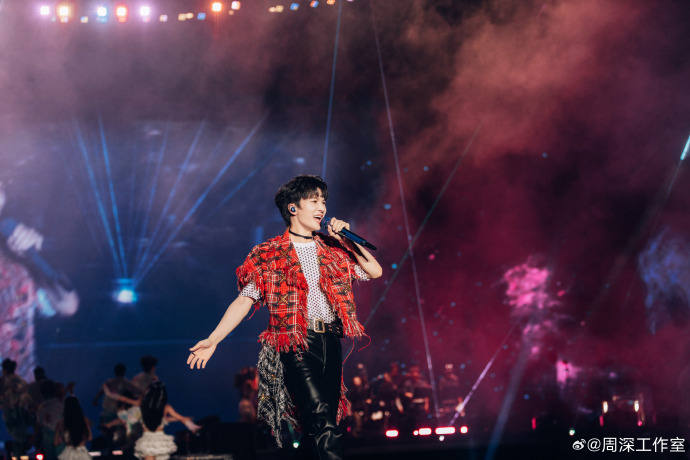
\includegraphics[width=400pt]{img/chengdu20240615/002} 

}

\caption{烦恼忧愁全部都抽空 【@weibo-charlie-studio】}\label{fig:unnamed-chunk-54}
\end{figure}

\begin{center}\rule{0.5\linewidth}{0.5pt}\end{center}

\begin{figure}

{\centering 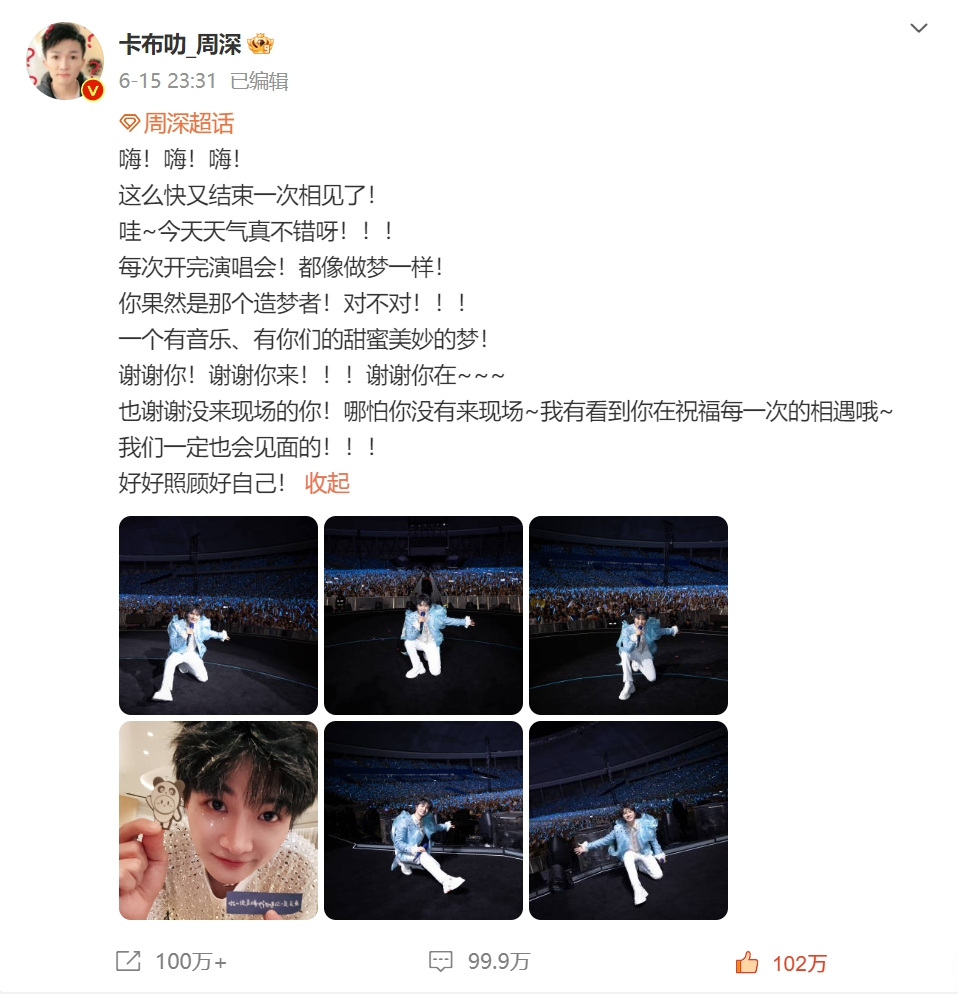
\includegraphics{img/weibo/chengdu-20240615} 

}

\caption{周深成都东安湖体育公园主体育场演唱会结束微博 【@weibo-charlie】}\label{fig:unnamed-chunk-55}
\end{figure}

\chapter{2024.07.13贵阳场}\label{guiyang-20240713}

\begin{quote}
\textbf{\emph{看到很多人在减少那个努力的重要性,但是我觉得我站在这里就证明努力是有用,周深可以,你也可以!------ 周深}}
\end{quote}

\begin{figure}

{\centering 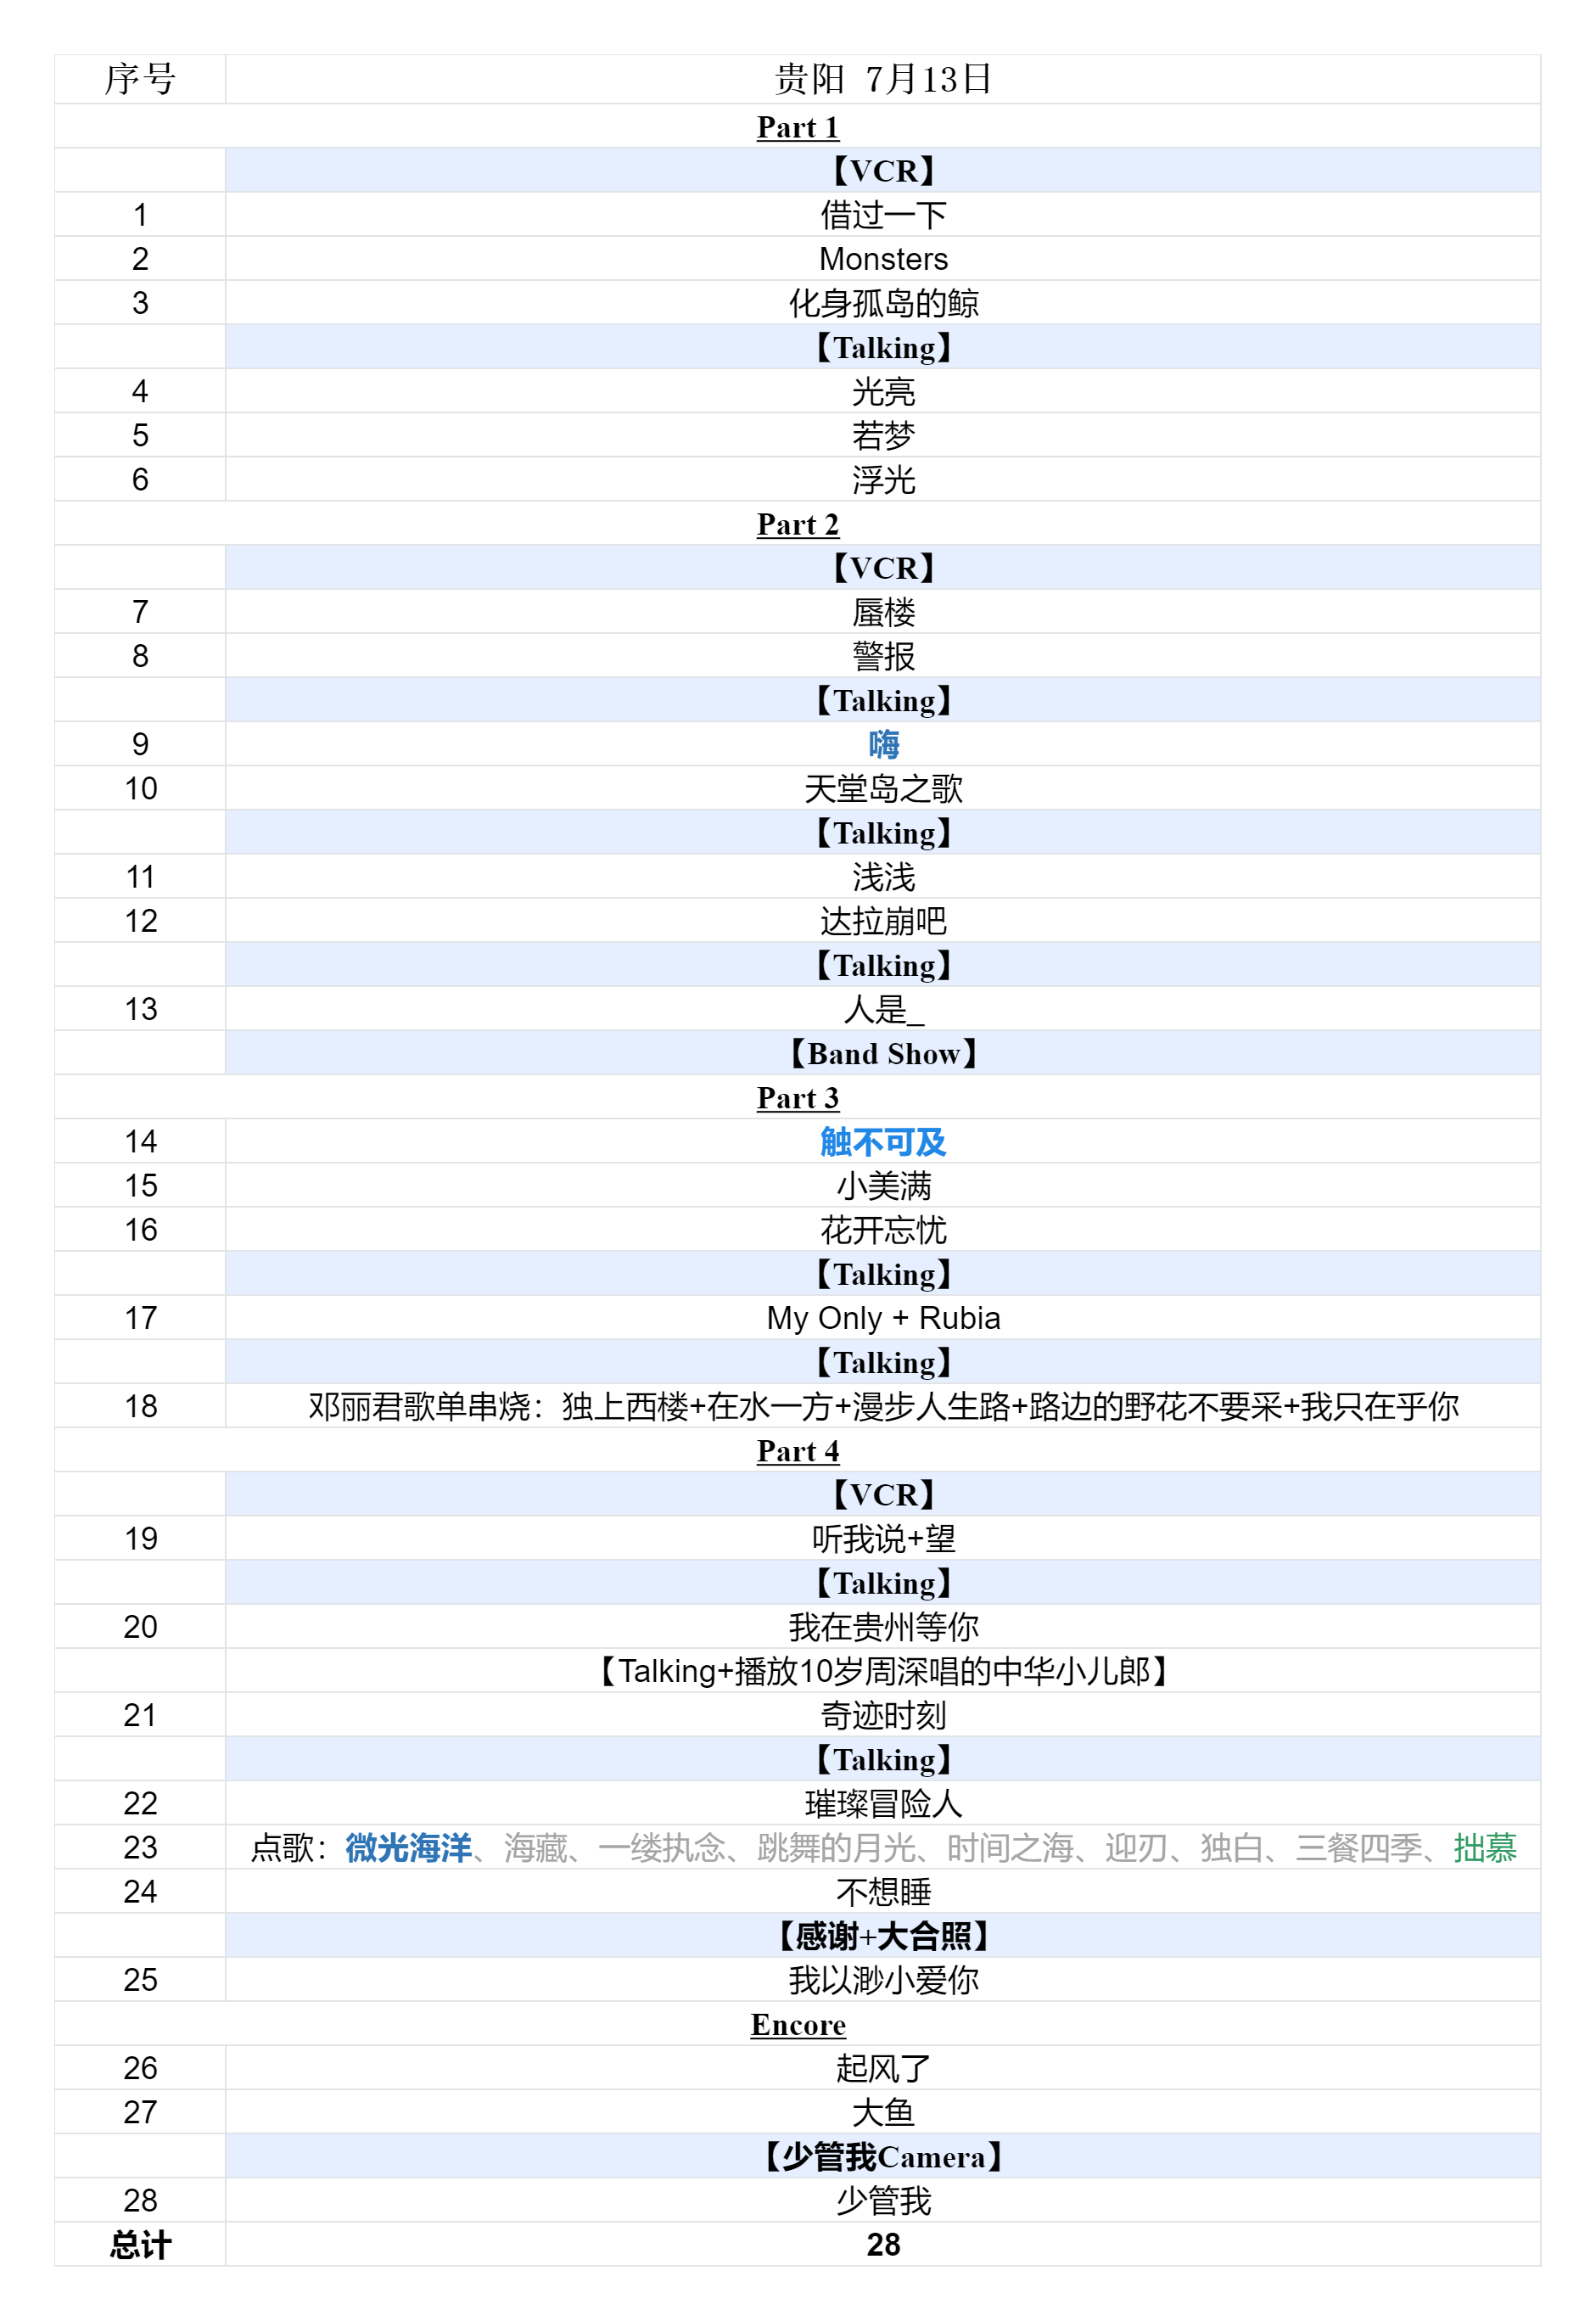
\includegraphics[width=330pt]{img/playlists/playlists-guiyang-20240713} 

}

\caption{2024周深9.29Hz巡回演唱会2024.07.13贵阳场歌单}\label{fig:unnamed-chunk-58}
\end{figure}

\newpage

\section{Part1}\label{guiyang-20240713-part1}

\hyperref[opening-vcr]{🎥【\textbf{开场VCR}】}

\hyperref[I-will-go-my-way]{🎵【\textbf{借过一下}】}贵阳的朋友,你们好吗?(米:好\textasciitilde)路借过一下\textasciitilde{}

\hyperref[Monsters]{🎵【\textbf{Monsters}】} \textbf{我一直都在哦\textasciitilde{}}

\hyperref[hua-shen-gu-dao-de-jing]{🎵【\textbf{化身孤岛的鲸}】}这首歌你们会唱吗?(米:会)那等下要跟我一起唱,好不好?(米:好)贵阳的朋友,你们好\textasciitilde 到你们\textasciitilde 麻烦这两位迟到的借过一下\textasciitilde(米:没有墙头)有墙头吗?那我可能要改个词了(深:我才不信你们都没有墙头,也希望你们都是,自己的王子、国王和王后)

  大家好,诶,贵阳的朋友你们好不好?看台的朋友们,你们好吗?那边看台的朋友们你们好吗?你们两位(帮忙换衣服)好忙,哈哈哈,他们都,我们今天,这里告诉我有4.2万的人一起在这里,一起去开心的度过这个演唱会。我想听一下大家一起说,唉,我想想说什么呢?我就问你们好不好?你们回答我好是什么样的音量?好不好?321,4.2万的朋友们,你们好吗?(米:好)哇塞,\textbf{你们声音太好听了},我想说我来贵阳的时候我特别紧张,因为这是我从小长大的地方,这是我从小到大的地方,我就觉得万一人家来没得照顾好人家。哼,我的贵阳话突然都不标准,万一没得照顾好人家,会不会不太好意思?这个贵阳话越来越不标准,会不会有点不太好意思,\textbf{但是我觉得我很幸福的是,谢谢贵阳所有的朋友们,无论是在现场,或者是没有在现场的大家,把大家都照顾得非常好,谢谢你们}。当然这里是不是还有很多从外地或者甚至是外国飞过来的朋友啊?贵阳凉不凉爽?(米:凉爽)贵阳天气好不好?(米:好)东西好不好吃?(米:好吃)贵阳人好不好?(米:好)刚我好像没有听到看台朋友的声音,我们让他们说一下,贵阳人好不好?(米:好)没错,所以我觉得自己很幸福,而且更大的惊喜是,哪怕就是我的生米们,真的让我,就很像别人来家里做客,会担心,诶,完了没有做好什么事。那你会发现生米们从其他地方来,把贵阳也增加了很多周深的一些元素或怎么样,把大家都照顾很好,我觉得你们比我更会照顾人,谢谢你们的爱,我都感受到了,谢谢你们。我时常会觉得自己很多时候,就一个人的时候,对吧,很孤单,但我会发现每次一回头有好多光啊,有好多光亮,\textbf{你们也经常说我照亮你们,其实是你们照亮我},谢谢你们每一份光亮。好紧张好紧张。

\hyperref[silver-linings]{🎵【\textbf{光亮}】}到你们(米:光亮你自己)

宝你个头,听古筝\textasciitilde{}

\hyperref[ruomeng]{🎵【\textbf{若梦}】}这首歌会跟我一起唱吗?\textbf{这首歌你们唱的特别好,比原唱好听多了\textasciitilde{}}太好听啦\textasciitilde 轮到你们喽(米:往事流转在你眼眸)这边的\textasciitilde 前面的\textasciitilde 我们一起,看台的\textasciitilde{}

\hyperref[floating-light]{🎵【\textbf{浮光}】}很感谢在这人生恍恍惚惚三万天当中遇到了你\textasciitilde{}

\begin{figure}

{\centering 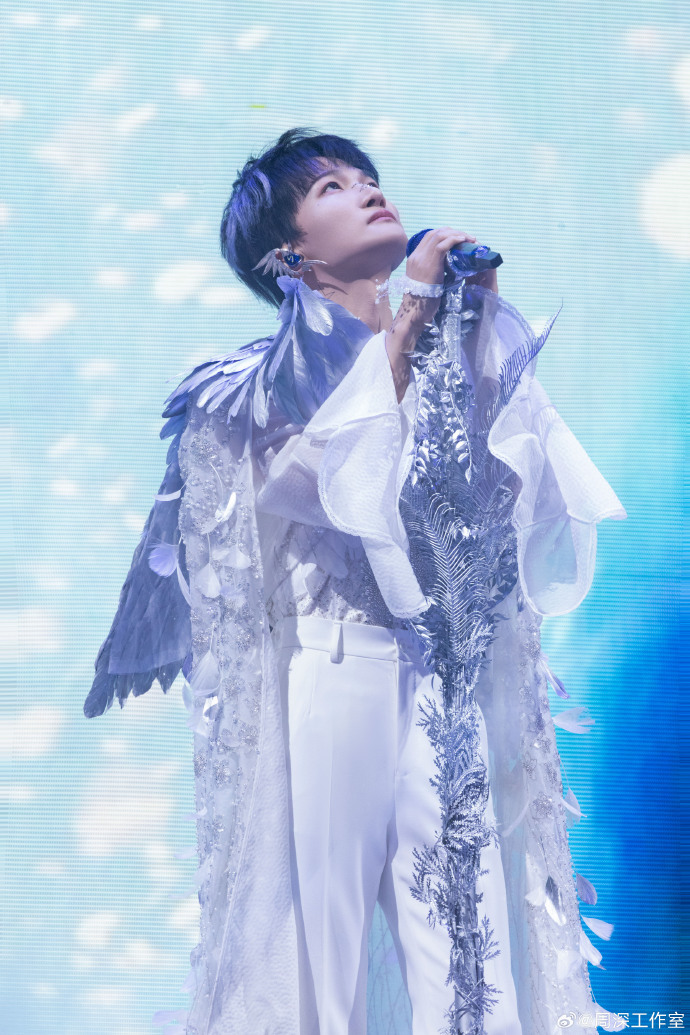
\includegraphics[width=400pt]{img/guiyang20240713/001} 

}

\caption{绝美 【@weibo-charlie-studio】}\label{fig:unnamed-chunk-59}
\end{figure}

\section{Part2}\label{guiyang-20240713-part2}

\hyperref[senself-vcr]{🎥【\textbf{反深代词VCR}】}

\hyperref[mirage]{🎵【\textbf{蜃楼}】}

\hyperref[the-giver]{🎵【\textbf{警报}】}谢谢大家\textasciitilde{}

  贵阳的朋友,你们好吗?(米:好)我觉得真的是太奇迹了,以前可能就在读书的时候,就可能老师们会说,如果有一天周深能够在贵阳大剧场演唱的话就非常厉害了,所以我在喜欢唱歌的时候,那个时候还没有奥体这个地方。总之就是你们好吗?我来啦!欢迎你们来到贵阳。刚才演唱的蜃楼和警报是新专辑(米:反深代词),好开心有那么多人知道我的新专辑,反深代词的两首歌。\textbf{这张专辑里面会有12个分身,不同的分身去感受不同的角度吧。蜃楼就是说很多人可能一些执念,可能自己会被困在那个执念当中,就希望如果是不好的执念的话,就让自己尽早的、尽量,就尽快的往前继续奔去。但也有很多好的执念会让自己变得越来越好,比如我想要跟你们见面这个执念。}第二个警报这首歌就是很多人,因为以前我觉得自己的性格是这样,而且我也相信有很多生米或者是歌迷朋友跟我一样,就很多可能觉得想要照顾好整个、所有人的情绪,但是这是不可能的事情,所以在做任何事情之前先要好好的照顾好自己,一定要看清楚警报的内容,好好的爱自己好吗?(米:好)然后接下来也请大家允许我再唱一首新专辑里的歌,可以吗?(米:可以)想了很久,但这首歌我发现他特别适合在贵阳唱,这是一首非常甜、充满爱的歌曲。为什么特别适合在贵阳唱?你知道为什么吗?因为贵阳人的身份证前三位是520,特别浪漫,就虽然我的身份证号不是520开始的,\textbf{但是我在贵阳也感受到了非常非常多的爱,然后也很幸运感受到你们给我的爱,让我慢慢可以站上舞台去感受每一份爱,也希望你们能够感受到身边更多的爱,好吗?(米:好)}看台的朋友,你们好吗,嗨\textasciitilde{}

\hyperref[say-hi]{🎵【\textbf{嗨}】}你们这么开心,你们会唱吗?(米:会)我不信\textasciitilde 全场跟我一起\textasciitilde{}

\hyperref[haven-song]{🎵【\textbf{天堂岛之歌}】}

  谢谢老师们。刚才我是不是有个动作,是(深:我逃不出去)\textbf{但突然就是一不小心跟舞蹈老师来一个十指相扣},哈哈哈,有那么些微的一丢丢尴尬,因为第一次我们,诶,我好像是在成都场的时候唱借过一下,然后那一下把老师的那个袖套刮走,有人看到吗?哦?那所以这里是有之前看过我演唱会的吗?那这里有没有是第一次看演唱会的呢?哇,哇塞,好开心,那就是,我没有想到这么多,总之非常感谢大家。那看台有没有第一次看我演唱会的呢?\textbf{我们一起创造这个非常非常美好的记忆好不好?(米:好)}刚才有演唱新专辑的歌嗨呀,蜃楼以及警报,当然所有的歌还在陆陆续续解锁当中,今天,应该是明天0点的时候,还会解锁一首新歌,也希望大家能够去听一听反深代词好吗?了解一下比较不一样的我,因为大家会觉得我比较古风,比较幽默,最可怕的是刚才那边喊出一个比较可爱,贼可爱。我这么酷跟可爱完全不沾边好吗?但是刚好我的一专里面有一首,诶,怎么说,很冷色调的一首歌,不知道你们会不会喜欢这首浅浅呢?

\hyperref[qianqian]{🎵【\textbf{浅浅}】}\textbf{我还没唱就哇,我唱了再哇好不好?}

  谢谢大家,说实话我从来没有想到夏天能够来贵阳开演唱会,也没有想到夏天开演唱会有点冷。我们一落地贵阳,我们就在想,哦吼,糟了,衣服改的越来越冷,结果来了贵阳场,怕是要被吹得抖起来,哈哈哈,就感觉衣服因为已经改得越来越凉快了,然后一来到贵阳,说实话这个风吹的我,刚才的那个颤音,有50\%是它造成,哦啊\textasciitilde{}

  那接下来这首歌该到你们唱,这是一个童话故事,知道是什么歌吗?(米:知道)但是有点提醒的是,荧光棒不要打到前面的,我已经陆续有看到,就是很多人的个子越长越高,哈哈哈,打着打着就越来越高了,所以一定要注意安全。然后那到底是谁救了谁?又杀了谁?又拯救了谁,又过上了完美的幸福生活呢?

\hyperref[dalabengba]{🎵【\textbf{达拉崩吧}】}

  谢谢,哇塞,我们贵阳的确是有点嗨爆,怎么感觉就整个人就是会兴奋的停不下来,就感觉会兴奋到失控,是不是因为你们太热情啦?但是我好像没有听到我们看台朋友的声音哦。我想玩一下那个声浪可以吗?就指向哪里?哪里就有声音,可以试一下吗?我有这个荣幸吗?试一下哦?那如果是这样呢(猫猫转圈圈)?谢谢你们,那接下来这首歌,我觉得是自己很幸福,可以唱很多电视剧、电影的歌,然后尤其是在电影院,就会听到,会说,``哇,好听'',哈哈哈,然后看到喜欢的电影,比如像泰坦尼克号,然后就会有立马就会想起很多经典的电影,那也希望自己以后可以用这样的方式去陪伴大家,无论怎么样,就是无论你在哪,我都在。这首歌希望你们喜欢,人是\_

\hyperref[renshi]{🎵【\textbf{人是\_}】}你们好吗?谢谢大家\textasciitilde{}

\section{Part3}\label{guiyang-20240713-part3}

\hyperref[untouchable]{🎵【\textbf{触不可及}】}会唱这首歌吗?(米:会)要跟我一起唱哦\textasciitilde 再来\textasciitilde 跟我一起(深、米:触不可及\textasciitilde)

  接下来这首就要一起唱喽,是什么歌呢?

\hyperref[happy-ending]{🎵【\textbf{小美满}】}跟我一起用最大的声音唱好吗?看台的朋友好吗?我要听一听我们4.2万人的声音有多大啊,这边\textasciitilde 那边的,看台的\textasciitilde 你们唱得太好听\textasciitilde 再来\textasciitilde 后面的\textasciitilde 谢谢大家,遇见你们是我今生最美最美的小美满,可以说是非常大的美满,所以每次听这首歌我就会觉得所有的愿望都会实现的。我们许愿不一定要在生日的时候,或者是在过年的时候,我们一起在小美满这首歌当中许一个愿望好不好?这是一棵许愿树,比如我现在许个愿望,321,你的愿望就会在我们许愿树上出现,所以我想现在每一个人都能听话,闭上眼睛,停止拍摄,然后我们慢慢地去想一个愿望,想你最想实现的愿望,好不好?然后喊321,最后再睁眼睛,大家闭眼睛开始许愿咯,想一想,诶,许什么样的愿望呢,想一想,诶,你最近想到谁呢?321,睁眼睛,所有的愿望都会在上面,都会被听见哦\textasciitilde 谢谢大家\textasciitilde{}

\hyperref[no-worries]{🎵【\textbf{花开忘忧}】}\textbf{谢谢你们跟我一起回家喽\textasciitilde{}} 你们会唱吗\textasciitilde 谢谢大家\textasciitilde{}

  这两天我有跟爸爸妈妈见,我就觉得,我爸爸妈妈就跟我说他们,我爸爸妈妈说最多就是,哇,好感动,有那么多人愿意陪你一起回家,看看你从小长大的地方。然后我特别想替我爸爸妈妈说一句,谢谢你们(米:谢谢周深)。然后刚才还有一个小小的小遗憾,就在小美满这个许愿当中,我一直都说很多时候大家都忘记了好好的爱自己,照顾自己。那刚才,我忘记跟你们说一个要求,就是我们的愿望必须要跟自己有关,我们重新许好吗?我相信如果听到了我们的愿望,我们冷烟花会再次燃起,我们一起闭上眼睛,只能够许关于自己的愿望,要好好爱自己,你有多久没有问自己一句,你还好吗?321,谢谢你们,无论你们在哪里,需要的时候我都在,谢谢你们。(米:谢谢周深)谢谢你们让一个非常非常普通的男孩从这里慢慢慢慢走到大家的耳机里,也非常感谢你们来看我,谢谢大家。

  好了,后面突然出现了一个很漂亮很漂亮很漂亮的区域。非常漂亮的树,在此之前我先脱了披风,哈哈哈。我有想到一个,诶,想到一个很好玩的事情,我有同学就是也是从外地来嘛,他就说,唉,你们贵州人说的好秋哦是什么意思?我想半天,什么意思?原来就是那个,唉呦,好求哦这个烟。哈哈哈,就是说很熏的意思,就如果在某个地方烟灰太大或者怎么样被熏着了,我们就会用贵阳话说,好求哦。好,接下来是两首,非常浪漫,非常温柔的两首歌,还是希望你们能够喜欢。

\hyperref[my-only]{🎵【\textbf{My Only}】} \hyperref[rubia]{🎵【\textbf{Rubia}】}等一下,这个戒指太重了,哈哈哈,让我重来一次好不好,戒指太重影响我发挥。哈哈哈,就是年纪一大把,我年纪也不小了,还要学一个新的事情,我觉得也很有乐趣。你们鼓励我好吗?谢谢你们,愿意捡起每一片不完美的我,你们好吗?

  真的很神奇,我也是第一次发现,原来我有那么多首歌是跟家有关的,还是说一次,谢谢你们陪我回家。(深深换服装,米狂欢)怎么有点手忙脚乱的,怎么回事?为什么现在的声音比我唱歌的时候声音还大声啊?那你们的意思是我以后就只要在上面换衣服就好了,不用唱歌。你们是从几岁开始听我唱歌的?根本听不清,哈哈哈,但是在之前深圳场或者成都场或者上海场都有很多小朋友们在现场,小朋友你们好吗?你们要好好的哦,然后对我影响最深刻的是我第一次听到唱歌,应该是邓丽君女士的歌声,你就觉得特别特别有感觉,有很多人听过他的歌,对吗?(米:对)所以我就希望自己能够成为像邓丽君女士这样的歌手,很多很多年之后,还是会有很多人想唱那个歌,很多很多年之后还有人听到她的歌的时候,一下就回忆起很多很多他们的往日时光,有美好的,有或者甚至是有一些许悲伤的,但是都不用害怕,因为她的歌声一直在陪伴。我想成为这样的歌手,我会继续加油的,我是歌手周深。接下来的歌如果你会唱的话,要跟我一起唱。如果你唱的比我好的话。那你上来唱吧,哈哈哈,希望你们喜欢,不是叫你们真的上来不要动。宝你个头\textasciitilde{}

🎵【\textbf{邓丽君组曲}】会唱的跟我一起哦,到你们\textasciitilde 这边的朋友\textasciitilde 会唱的一起唱哦,这边的朋友\textasciitilde 你会唱吗?不采就是不采哦,不能出去采哦\textasciitilde 你们会忘记我吗?谢谢我的每一个生米,谢谢,谢谢你们\textasciitilde{}

\section{Part4}\label{guiyang-20240713-part4}

\hyperref[thank-you-vcr]{🎥【\textbf{谢谢贵阳,谢谢你VCR}】}

\begin{figure}

{\centering 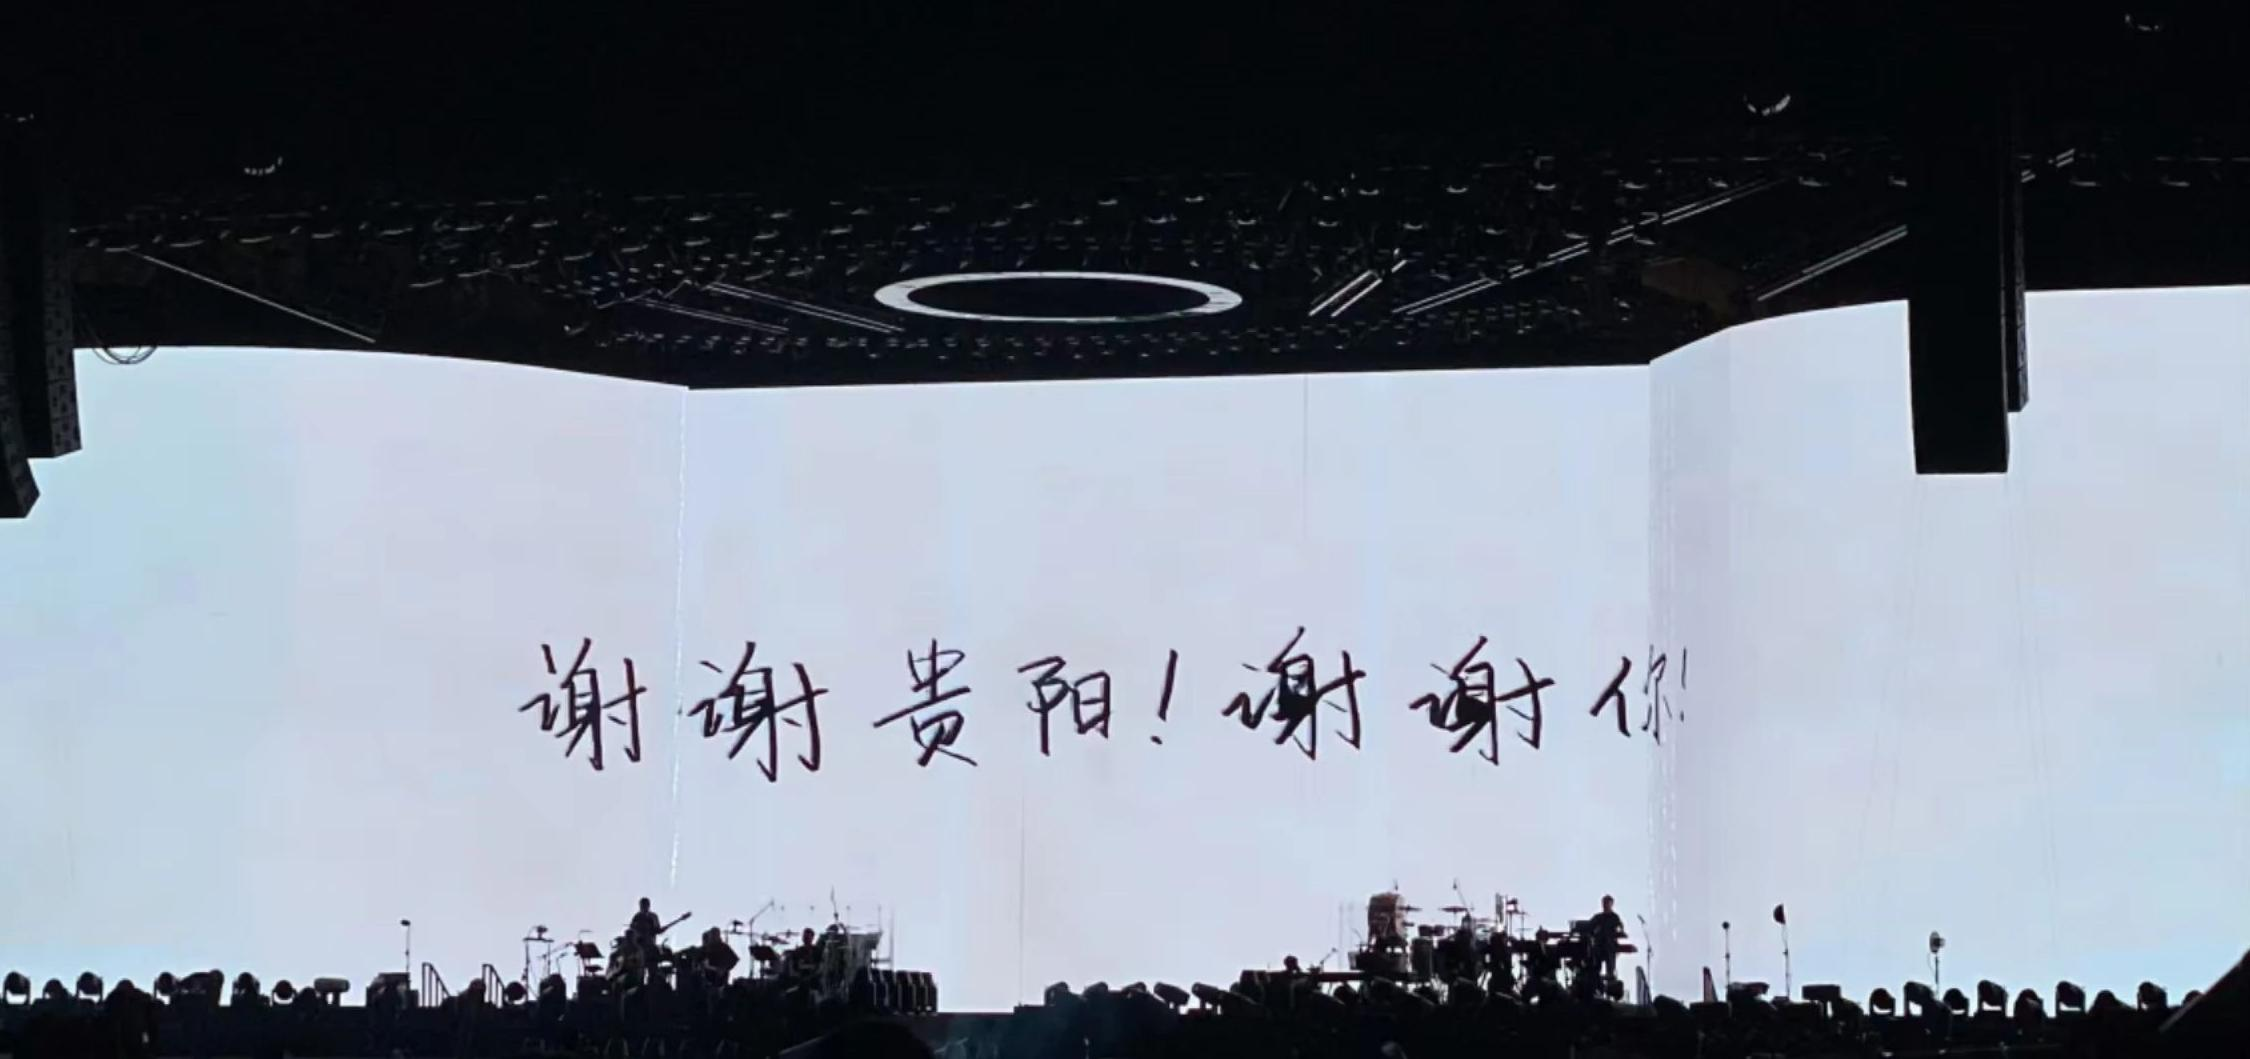
\includegraphics[width=400pt]{img/guiyang20240713/thank-guiyang} 

}

\caption{谢谢贵阳!谢谢你!}\label{fig:unnamed-chunk-60}
\end{figure}

\hyperref[listen-to-me]{🎵【\textbf{听我说}】}谢谢贵阳,谢谢你\textasciitilde 谢谢你们,我们一定都会越来越好的\textasciitilde 到你们\textasciitilde 那个人也可以是我吗?

\hyperref[hope]{🎵【\textbf{望}】}因为有你你你你你你你你你你你你你你你你你\ldots 你,(深:我才心有所住)

  谢谢大家,大家都知道贵州是有非常非常多少数民族的,(米:宝贝)宝你的头乘以4.2万。大家是不是知道贵州有非常多少数民族呀?所以在我们贵州无论是吃的或者是穿的,或者所有的感受或者是音乐都非常的多样性,然后以前就会经常发现自己同班同学有很多像布依族或者是其他民族的同学们,然后我也非常开心请到了我们的侗族和苗族的小朋友们跟我们一起唱歌,大家等一下要用最大的掌声欢迎他们哦。我们演出这首歌叫做《我在贵州等你》。

\hyperref[waitting-in-guizhou]{🎵【\textbf{我在贵州等你}】}小朋友们唱的好不好听?(米:好听)到你们\textasciitilde 全场\textasciitilde{}\textbf{欢迎来到贵阳,我们来一起蹦苗迪好不好},等下你们跟着我一起喊,我喊什么你们喊什么好不好?我在,要大声点哦,123,走,我在(米:我在),我在(米:我在),我在贵(米:我在贵),我在贵(米:我在贵),我在贵州(米:我在贵州),我在贵州(米:我在贵州),我在贵州等你(米:我在贵州等你)\textasciitilde 看台的朋友,嘿嘿嘿嘿嘿\textasciitilde 全场,嘿嘿嘿嘿嘿(米:嘿嘿嘿嘿嘿)我们在贵州(深:等你)

  谢谢,掌声给我们侗族的小朋友们、苗族的小朋友们,掌声再热烈一点,谢谢你们,啊,谢谢,(小朋友站着不动等人领下台)那舞台给你们,她们太可爱了,小朋友们唱得好不好?她们一出来的时候,我感觉自己在多彩贵州风的演唱会上,好了好了,谢谢你们哦,谢谢你们。好嘞,谢谢大家,然后非常感谢大家来贵阳跟我们相遇,今天对我来说其实非常紧张的一场。因为以前就感觉在开演唱会,然后这一场其实就有自己的家人,然后也有我的,有高中老师,有初中老师,还有小学老师,他们都在,对于我来说这更像是一场汇报演出。你们孩子这几年在外面还可以,哈哈哈。然后有很幸运的是有那么多人愿意陪我一起来贵阳看你们。那么对于我来说也有一个非常大的惊喜,就是我没有想到能够这一次,我的小学老师,就第一个发现我能够唱歌的那位老师,张老师,然后她就说,张老师,她就说,你知道吗?你03年的时候录的一首歌,我这里还有磁带。我也是昨天才知道这个消息,我非常感动她一直保存好这一场磁带,但是我也在心想,如果唱的不是很好,我就去把那磁带再毁掉。所以可以耽误大家一点时间听一下21年前的周深唱歌是什么声音吗?好了,安静哦,321,声音可以再大一点点【中华小儿郎】你们觉得唱得还可以吗?哇塞,我们就不聊这个了,哈哈哈,我是没有想到,哦,我老师在这,谢谢张老师,我这个不让下来,会不安全,什么?我知道是张老师给我录的,谢谢张老师。谢谢谢谢谢谢。那我觉得还有一点很重要的,就是我的初中老师或者高中老师,他们从来没有跟我说过一次你唱音乐不好,或者是音乐会耽误你什么什么的,所以我觉得自己是一个很幸运的事情,啊哈?自己是一个很幸运的人,就是一路上有很多人温暖的陪伴着我,然后因为一定有很多人可能遇到过一些极端的老师,那我觉得自己很幸福的人,也希望能够把这个幸福传递给大家,因为我们可以创造更多的奇迹,周深都可以,你们一定也行。

\hyperref[magic-moment]{🎵【\textbf{奇迹时刻}】}【魔术时间】Ladies and gentleman,掌声在哪里?

  哈哈哈哈,我的魔术变得还好吗?(米:好)你们真是好人。好,非常感谢张老师,谢谢谢谢,也谢谢到来的所有每一个你,谢谢谢谢,因为安全问题,没法给个拥抱,但是谢谢张老师,要用更大的声音感谢每一个你,还包括看台的你。而且我有听说好像场外也有很多人在听,跟我们一起创造美好回忆,我们一起谢谢他们,123(米:谢谢)。大家一定一定一定要注意安全,安全第一好吗,(米:好)我觉得这次我回到了我所有,应该算是人生的起点,我一直在,就怎么说呢,很多时候在自己成长过程当中一定也有很多冒险嘛。比如,之前选择想要当一位牙医,我觉得对我来说可能是一个不太正确的选择,但是在其中,我也锻炼自己很多一些性格或者品性,我为什么要说这些?因为最近是不是有很多人刚好高考毕业?\textbf{我想要跟你们说,就是年轻就是你们最厉害的资本,你们随时可以去尝试,可以去找寻那个最好的自己,找到那一条路,然后努力去奋斗,你们也可以成为那一个璀璨冒险人。}

\hyperref[adventurers]{🎵【\textbf{璀璨冒险人}】}因为我有看到很多很多,就是因为是信息时代,可以看到很多人在减少那个努力的重要性,但是我觉得我站在这里就证明努力是有用,周深可以,你也可以,对吗?(秒进歌曲,深:这个世界是什么摸样)你们都是自己的英雄\textasciitilde 一起\textasciitilde{}

【\textbf{点歌环节}】谢谢老师们,现在我们到点歌环节喽。不要高兴的太早,因为可能那些歌你没有听过,但是我自己喜欢的歌有太多太多了,一场演唱会没有办法全部把它安排起来,就请允许我把很多歌都放在点歌环节,好吗?(米:好)我们现在要全场倒数5个数字,然后如果最后我们的摄像机拍到哪位朋友,那就是哪一位朋友来点歌。你,诶,那写个加场,我已经在加场了,哈哈哈。我从来没有想过自己能够在体育场开演唱会,也没有想过大家希望加场。还是那句话,谢谢每一个你。来喽,全场要帮我倒数5个数字好吗?(米:好)我们的屏幕滚动起来,诶,现在只看到了我,来了全场,呜,好多朋友啊,来喽,宝你个头(看到横幅``宝我个头''),怎么还自己宝呢。来,全场,5(米:4321),芜,啊,这里。小朋友你好(周深哥哥你好)好久没有听到这么亲切的童声叫周深哥哥,哈哈哈,现在在外面,大部分都叫周深叔叔。你好(你好),应该怎么称呼你?(你可以叫我小崔)小崔,哈哈哈,我可不得叫你小崔嘛,那平时你家人也这么客气叫你小崔吗?(一般我的老师叫我小崔)我,好的,原来现在我是你的老师的位置,好的,那,作业做了吗?哈哈哈,放暑假呢,你现在几岁啊?(现在11岁)11岁,哦,那你几岁开始听我的歌?(从7岁开始)7岁开始听,哦,是谁给你听我的歌?是家长还是?(主要是刚开始是我的妈妈)啊,您好您好您好(小崔妈:周深宝贝)哇,小崔,我是你,我可就酸溜溜的了,哈哈哈,那你看看上面有9首歌,有没有你想要听的?(都想听)都想听?这个答案是无效的答案,来,换一个(那就微光海洋吧),小崔好眼光,非常开心的一首歌,送给你,也送给大家,微光海洋。谢谢小崔,小崔,这么叫太客气了,家里人怎么叫你啊?家里人没怎么叫你,难道妈妈也是平时说小崔吃饭啦。妈妈叫什么?(小崔妈:妈妈叫果儿,我的网名叫果儿\textbf{宝贝}妈咪)微光海洋,送给大家。

\hyperref[sea-of-shimmer]{🎵【\textbf{微光海洋}】} 谢谢,谢谢小崔,谢谢你的家人,以及谢谢大家。宝你个头宝你个头,我们重来这首歌,怎么回事,宝你个头,但是怎么,怎么在看台的朋友不叫呢(米:宝贝宝贝)宝你个头乘以4.2万,好,微光海洋。有听过这首歌的吗?那要跟我一起唱哦\textasciitilde 谢谢你们,也希望我的歌声能够化作大自然间的每一样东西陪伴着你们\textasciitilde{}

\hyperref[keep-playing]{🎵【\textbf{不想睡}】}到你们\textasciitilde 谢谢你们来,谢谢你们,谢谢你们\textasciitilde 全场跟我一起\textasciitilde 看台的朋友\textasciitilde 再大声一点\textasciitilde 好好听啊,谢谢大家\textasciitilde{}

  好,那,不知道这里有没有人知道一个叫做卡布的人呢?卡布是我以前就是自己喜欢在家录歌,然后发到网上去,然后,的那个马甲,所以很多人可能像听到化身孤岛的鲸,第一次听到那个时候就是卡布唱的,所以非常感谢。刚才那首歌也是卡布的晚安曲,就是说我们演唱会快到尾声喽。大家觉得好听吗?(米:好听)我非常喜欢这一次我们的相遇,所以我们要非常感谢让我们安全、开心享受今天晚上的所有的工作人员们,好吗?(米:好)

  我们感谢贵阳市人民政府,感谢贵阳市公安局,感谢贵阳市文化和旅游局,感谢贵阳市消防救援之队,感谢观山湖区文体广电旅游局以及所有相关部门的大力支持,谢谢他们,感谢场地支持,贵阳市旅发集团。感谢我们这一次巡演的全程主办北京时代立方文化传播有限公司,我们非常非常感谢他们,因为我们每次回去,我们的主办,他们会主动想我们哪个地方可以更好的让我们的观众,去照顾到他们,所以希望,我们肯定不会做到完美,但是我们一直在用心,希望大家能够感受到我们主办以及我们所有老师们的用心,也谢谢你们来。感谢演唱会制作单位必应,感谢总导演周佑洋、庄惟惞,大家今天听我的声音好听吗?(米:好听)之所以那么好听声音也要感谢我们的音响总监金少刚老师,感谢我们的音乐总监龙隆老师,还有掌声送给我们今天的乐队老师们,以及我们乐队老师当中我们的贝斯老师,也是贵阳的哦。我们一起欢迎欢他回家,123(米:欢迎回家)呦吼,好,感谢我们的舞蹈团队SDT ShowPro。以及感谢我们刚才特别可爱的孩子们,山娃娃合唱团,以及贵州云上侗寨小歌队。感谢我们的服装团队设计师劳伦斯许工作室,感谢时装品牌windowsen,感谢我们的音响工程南京奥斯泰视听科技有限公司,感谢我们的调音团队乐尔工作室。大家感谢累了吗?(米:没有)哎呀,你们真的是太好了,谢谢你们,来,谢谢我们的硬体工程,北京力超舞台集团,感谢周深工作室的小伙伴们。哈哈哈,谢谢大家,我其实就非常清楚,因为大家看到的都是我,大家感觉到就是,啊周深你是光,或者是我自己很幸运感受到大家给我的光,但其实后面也有很多我们工作室的小伙伴们在慢慢的把我想要传递出去的信息或者所有的东西去传递给大家,所以非常感谢他们,就是也感谢所有老师们,可以促成我们这一次非常美好的相遇,谢谢。感谢微博(米:倒闭),感谢微博音乐(米:倒闭),感谢,我感谢你们,感谢微博演出(米:倒闭),以及感谢现场所有的工作人员们,\textbf{最重要最重要的是感谢每一个来到9.29Hz贵阳场的你。}

  所以,我们来大合照吧,我们先是中间的呦,好,场灯可以亮一下,谢谢,好,321,好,我们左边的朋友们,321,右边的朋友们,哇,做这个蹲脚的姿势,脚不能直哇,321,好,那边的朋友,对不起啊,耽误大家一点时间。好了,大家都可以看到哦,来喽,那边的朋友,我来啦,我歇会再来,我又来啦,我再歇会,原来跑步这么累啊,你们好,321,好,谢谢老师。那接下来这首是属于周深的晚安曲,我以渺小爱你。

\hyperref[loving-you-in-my-humble-way]{🎵【\textbf{我以渺小爱你}】}谢谢你们看到了渺小的我哦\textasciitilde 谢谢你们,谢谢你们不嫌弃我的力量不够强大,谢谢你们,谢谢,谢谢大家,谢谢你们,\textbf{我们回家喽\textasciitilde{}}

\section{Part5}\label{guiyang-20240713-part5}

\hyperref[the-wind-rises]{🎵【\textbf{起风了}】}贵阳的朋友,你们好吗\textasciitilde 后面的朋友\textasciitilde 谢谢你们\textasciitilde 如果你们说我可以飞,那是因为你们是那一阵爱的风。

\hyperref[big-fish]{🎵【\textbf{大鱼}】}

  谢谢大家,谢谢,谢谢你们愿意听我唱歌,谢谢你们愿意在这里听我唱歌,谢谢你们愿意听我唱歌。最后请允许我耽误大概几分钟,因为我还要唱一首新专辑里的歌,叫做少管我,少管我,大家有的时候会听起来感觉像是争执,或者像是在吵架的时候会说的话,但其实不是,因为在我心中大家可能看到过古风的我、缥缈的我、高冷的我。但是怎么说呢?我觉得一路走来,\textbf{周深最清楚的是周深知道该怎么去做周深喜欢的那个自己,这是我理解的少管我。}少管我就是自己要对自己负责,所以我相信你们一定也可以找到那个你最喜欢的那个自己的,可能会走一点点小的弯路,但是没有关系,那个你喜欢的自己在未来等着你。少管我,我们有一个自己的小小的一个特别的手势,就是嘿,少管我。这里有人听过少管我吗?嘿,少管我,还是一样的,我们这里会有个少管我camera,就是拍到谁就要帮我们做这个,嘿,少管我,以及喊出你最大声音的,少管我的音量好吗?还是一样,注意安全,不要打到前面的朋友的脑袋来,我们全场依然倒数5个数字,我们的摄影老师转起来吧,全场5(米:4321)停,那既然这样,两位男孩和女孩,那既然有三个,那就三位吧。哈哈哈,好好,那我们先女生好不好?好好,特别漂亮的这个,都很漂亮,那该怎么形容这个发型呢?这个叫什么发型啊?披着的这个发型,应该怎么称呼你?红米?这是你正儿八经的名字吗?嘚嘚嘚嘚,那大家一般会怎么称呼你?没有这个,你从哪里来?你从成都来?我刚刚从成都开完演唱会过来,你晓得不?哦,你也在,那你会说这个嘿,少管我吗?要喊出最大声音哦。来,321。她优不优秀,好,谢谢你,谢谢你,谢谢红米,既然你说这样叫你的名字的话。

  那这位头发扎起来的这个女生。就是你,没错,就是你,您怎么称呼啊?董?同?董?又是一位董小姐。好,您好,您是哪的人呢?宁波?哈哈哈,\textbf{关于宁波这个地方我熟悉,经常能听到您拨打的用户正在通话中,哈哈哈},你说来宁波开演唱会是吗?我加油,因为毕竟也不是我想开到哪里就可以开到哪里。好,现在要用你最大的声音喊出这一句,把所有不开心喊开,好不好?321,就四个字也要考虑歌词吗?哈哈哈,我们再来一次321,嘿,哇,真棒。好,我们后面都一直拿着手机的这个男生,怎么称呼你?默默?好可爱的名字,你是从哪里来的?湖南?我是湖南出生的。好嘞,那你从几岁开始听?哈哈哈,你从几岁开始听我的歌啊?5岁,哈哈哈,我也没出道这么多年,哦,听我的歌五年了?那你要喊出这一声哦,好,来,怎么称呼你来着?默默,好勒,321,手势不对,嘿,少管我,来321,哈哈哈,谢谢,你们不要笑别人,我们全场,321,(米:嘿,少管我)谢谢,所有的不开心都会离你们远去的。

\hyperref[watch-ur-manners]{🎵【\textbf{少管我}】}54321,全场\textasciitilde 全场\textasciitilde 谢谢你们来,你们想成为谁都可以,想成为什么颜色的自己都可以,祝你们天天开心,全场\textasciitilde54321,你们一定会成为你们发光的自己的,谢谢,谢谢你们来,谢谢你们在。好好照顾好自己,东西不要掉了,手机、证件、人身安全,都要好好的回到家好吗?后面的朋友,照顾好自己哦,听到了吗?谢谢你们来,54321\textasciitilde 贵阳的朋友们,再见\textasciitilde 谢谢,谢谢你们,谢谢,注意安全,东西别掉了,谢谢大家!54321,\textbf{你们是最棒的!}

\begin{center}\rule{0.5\linewidth}{0.5pt}\end{center}

\begin{figure}

{\centering 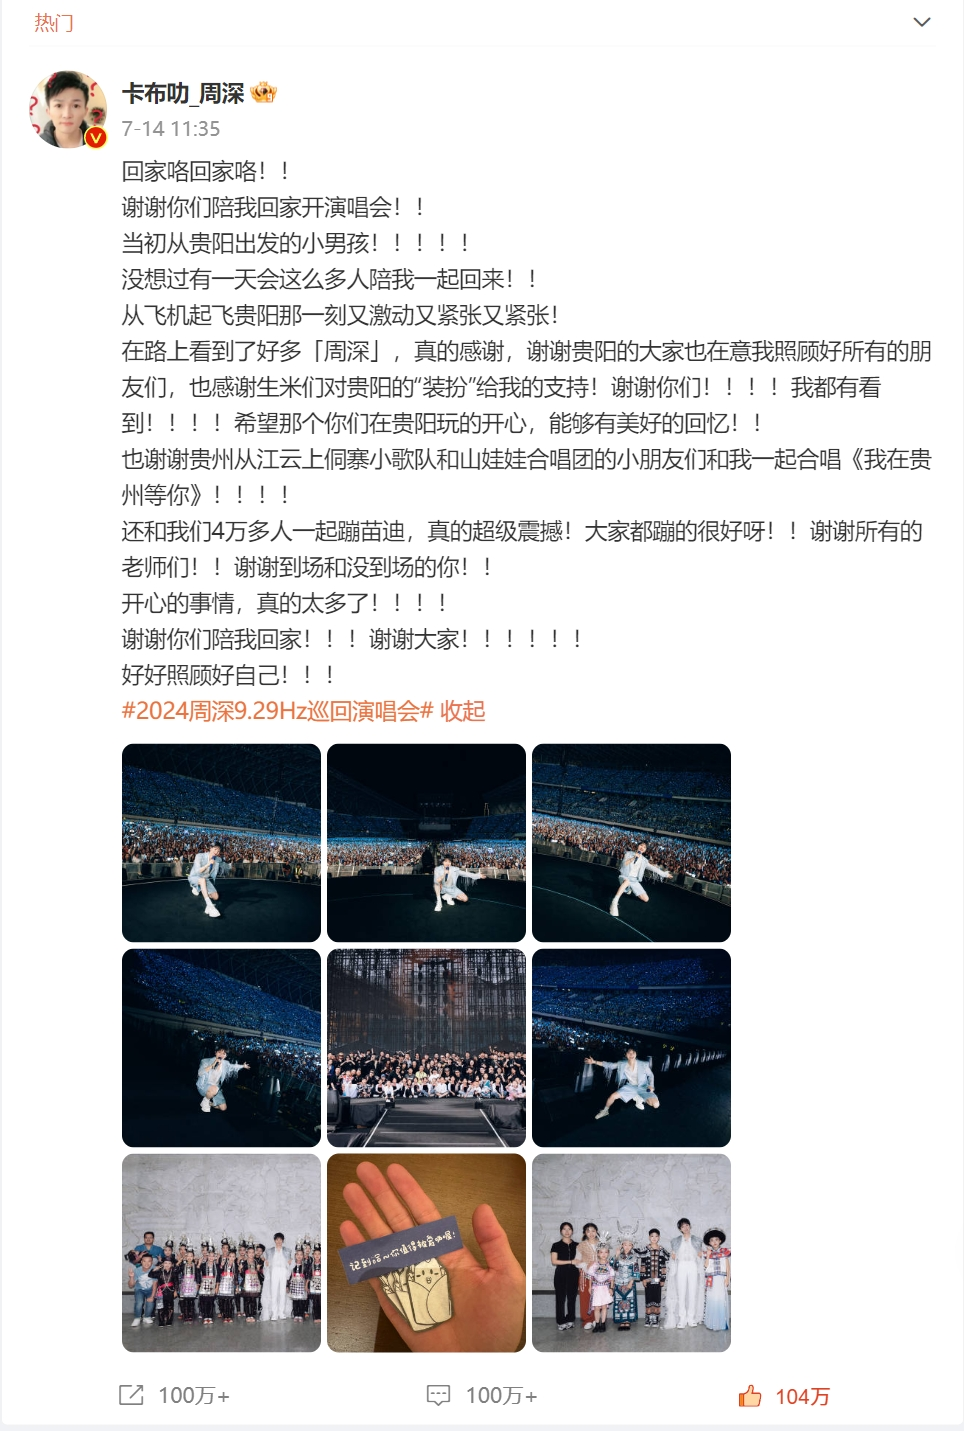
\includegraphics[width=350pt]{img/weibo/guiyang-20240714} 

}

\caption{周深贵阳奥林匹克体育中心体育场演唱会结束微博 【@weibo-charlie】}\label{fig:unnamed-chunk-61}
\end{figure}

\chapter{2024.07.27武汉场}\label{wuhan-20240727}

\begin{quote}
\textbf{\emph{完了,一起淋过雨的人,你就要记住我一辈子喽。------ 周深}}
\end{quote}

\begin{figure}

{\centering 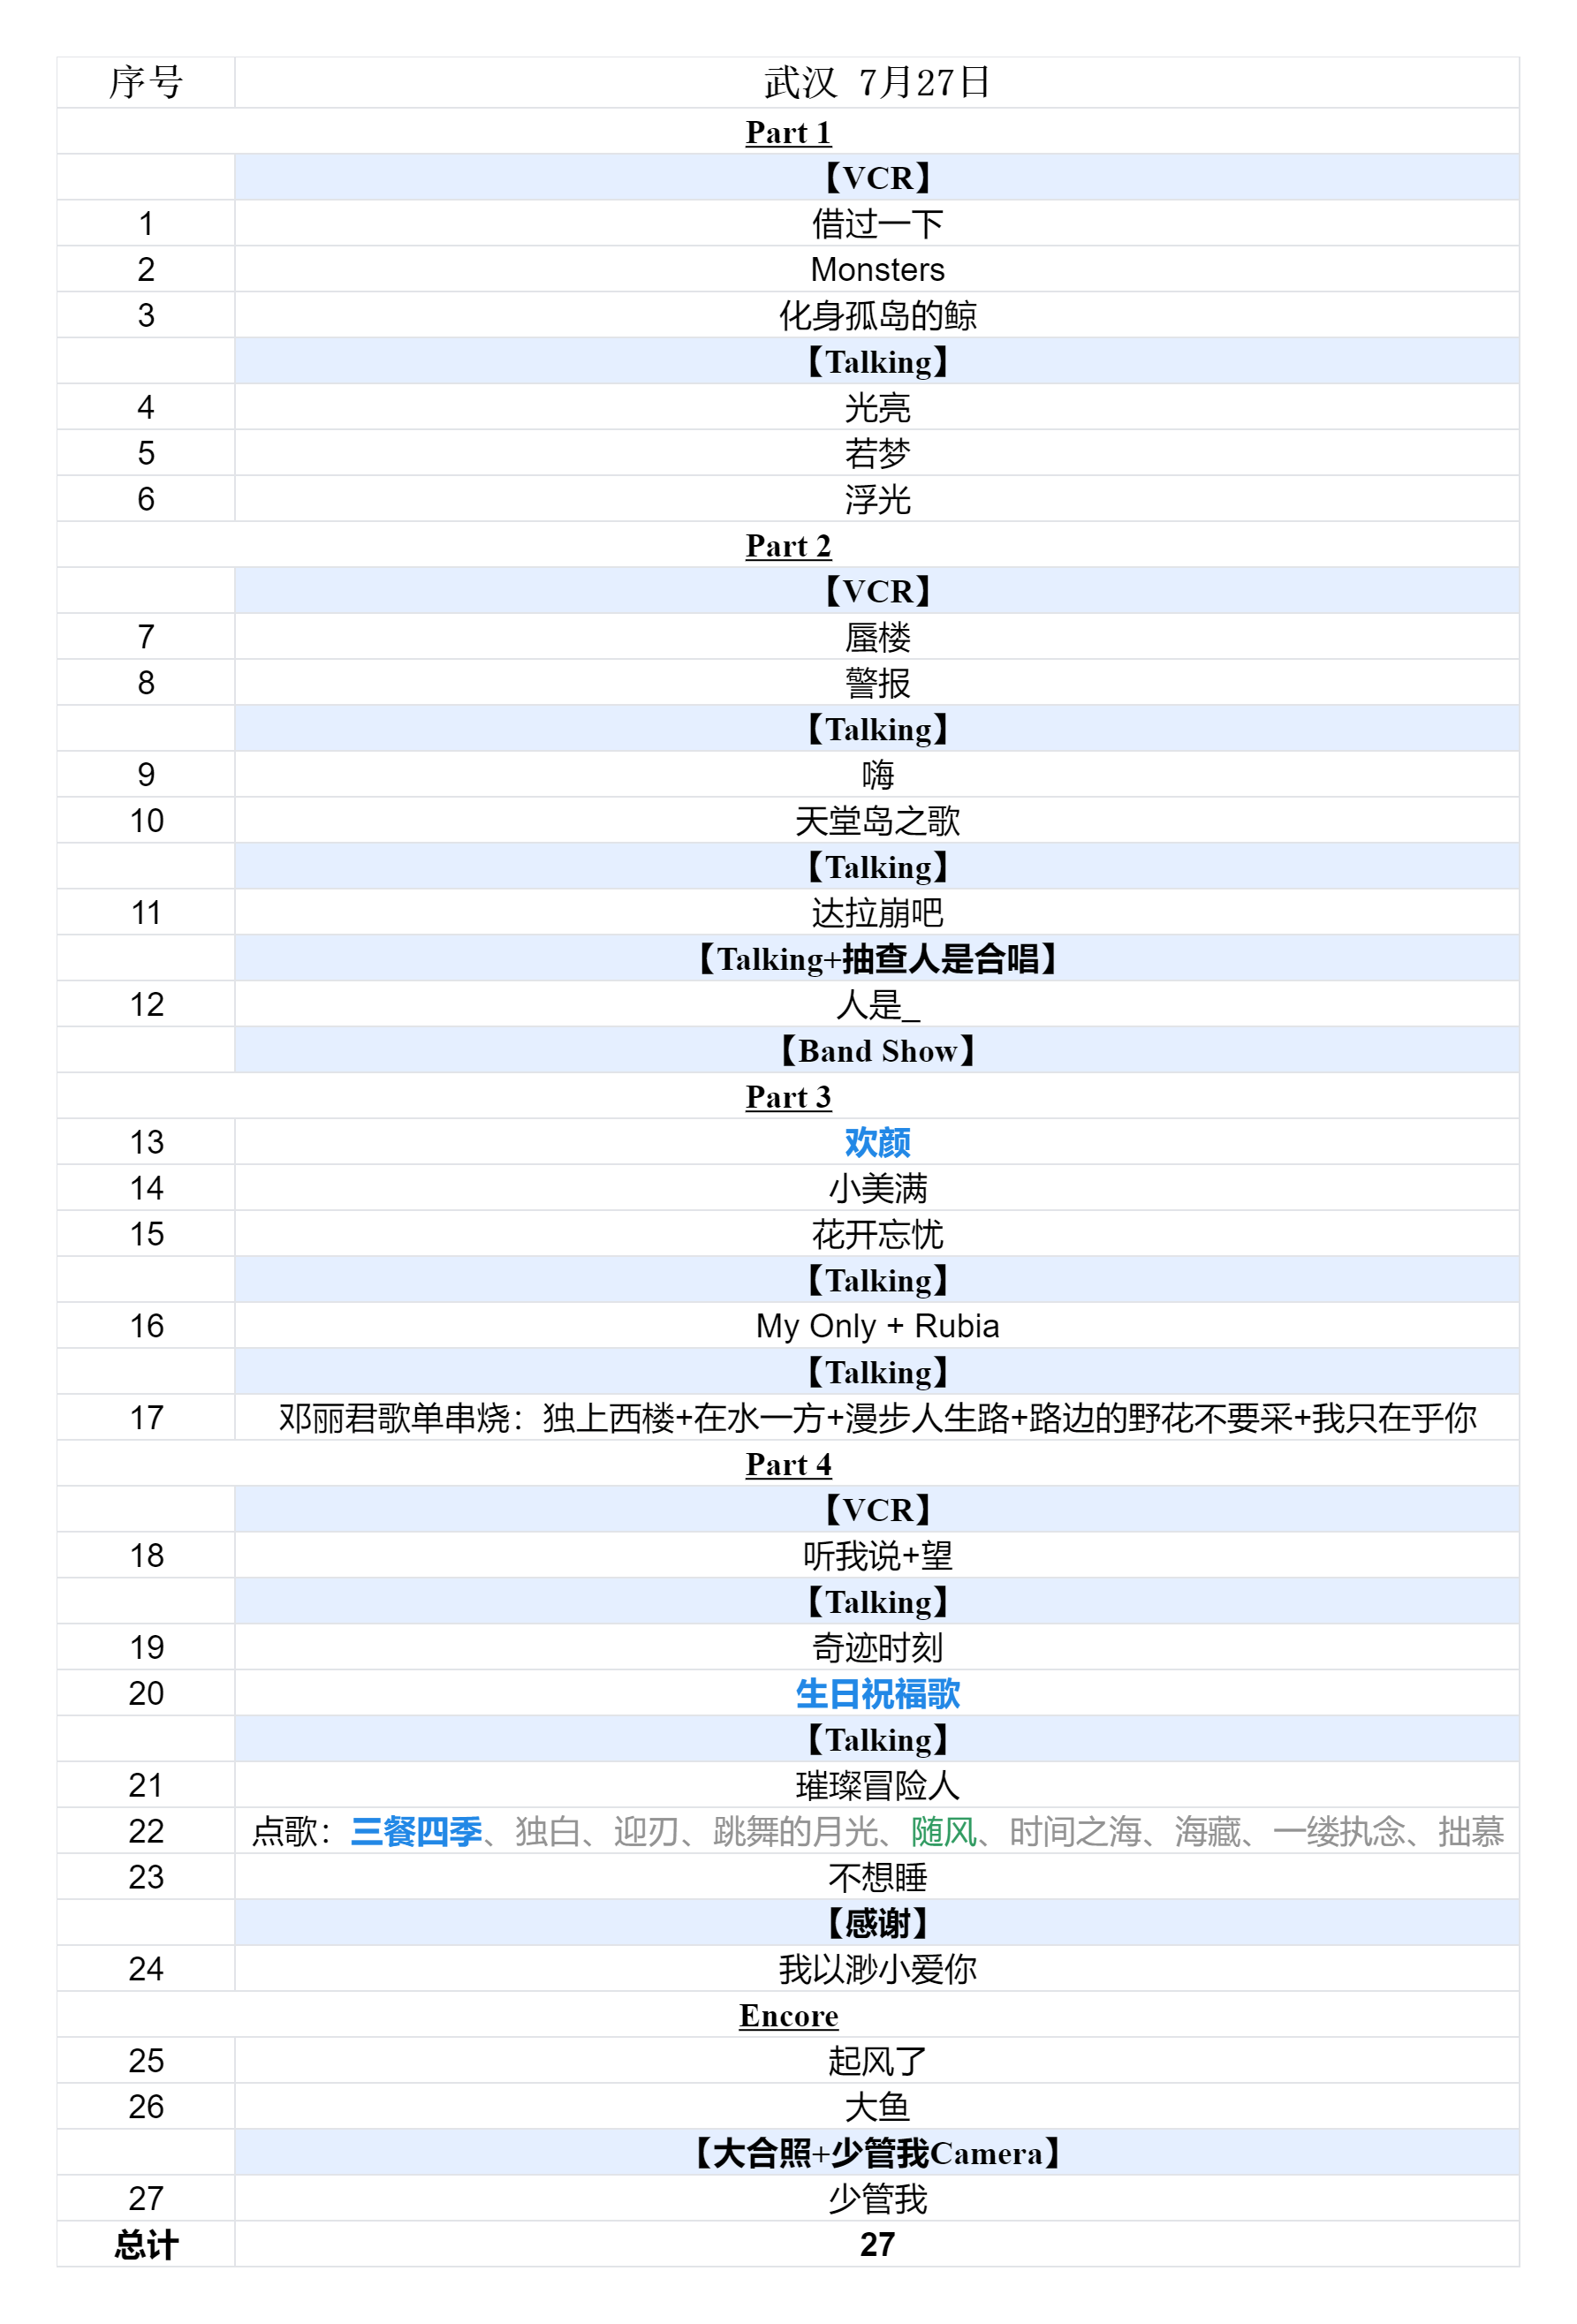
\includegraphics[width=320pt]{img/playlists/playlists-wuhan-20240727} 

}

\caption{2024周深9.29Hz巡回演唱会2024.07.27武汉场歌单}\label{fig:unnamed-chunk-64}
\end{figure}

\newpage

\section{Part1}\label{wuhan-20240727-part1}

\hyperref[opening-vcr]{🎥【\textbf{开场VCR}】}

\hyperref[I-will-go-my-way]{🎵【\textbf{借过一下}】}武汉的朋友,你们好吗?你们好吗?愿意跟我一起吗?

\hyperref[Monsters]{🎵【\textbf{Monsters}】}

\hyperref[hua-shen-gu-dao-de-jing]{🎵【\textbf{化身孤岛的鲸}】}这首歌会唱吗?(米:会)。会愿意跟我一起唱吗?(米:愿意)\textbf{今天我又要变矮了}。这边的朋友\textasciitilde 大声点\textasciitilde 你们好\textasciitilde!到你们\textasciitilde 大声点\textasciitilde 这里写了一个,你才有墙头,是的,我是有墙头。你们有墙头吗?没有,(深:我才不信你们都没有墙头,但是你们依然是国王或者是王后)。

  大家好,我是歌手周深,你们好吗?(米:好),我们终于见面了。哎呀,吓我一跳,我想说非常非常的有缘分,我跟武汉非常有缘。没有记错的话,我应该是第六次来到武汉,而且前两天,就7月25号的时候是歌手周深正式出道的第十年,所以谢谢你们能够听到一个歌手叫周深,谢谢你们。还有一个特别的缘分,就是当歌手周深出道之后,然后我们会有一系列,就节目的一些宣传活动嘛。我当时的第一个活动,也就是第一次以歌手周深这个职业来跟大家见面的时候,就是在武汉,当时是在光谷步行街,是不是有个地方叫光谷步行街?(米:有)wu\textasciitilde,今天是不是有好多武汉的朋友?(米:是)谢谢你们,有没有外地的朋友呢?(米:有)那我真的很想说一句,就是真的真的辛苦大家了,谢谢,谢谢,谢谢你们来赴约,谢谢,谢谢,谢谢。因为,就是因为有台风嘛,然后就可能有一些航班就可能会稍微延误,或者是有些那个车就会延误,但是还是非常感谢你们来跟我见面,谢谢你们。\textbf{今天也有一些小小的原因,我们的延伸台也没有像以前一样稍微的延伸长一点,所以我会担心我的感谢和我对你们的爱,我能不能够延伸到我们的看台朋友那?(米:能)那边我可以延伸过去吗?(米:可以),谢谢,谢谢,谢谢。}然后今天的舞台也没有像以前的那么大,所以我觉得今天非常非常的特别。我当时在,第一次就在武汉我们路演的时候,我们那个舞台的大小可能就跟我们一个键盘老师的,就大概就是我们乐手区那么大,所以我感觉应该是时刻在提醒我,歌手周深是从哪里出发的?歌手周深是怎么走到大家面前和进入到大家耳机里面?唯独只有那一声我会记住的,以及非常非常感谢每一个听到我的人,谢谢,谢谢,谢谢。

  稍等,我学了一句武汉话,武汉的朋友们,你们好。然后,稍等,你们吃了没?你们以后都可以叫我拐子,哈哈哈。是这样说的吗?不能叫宝贝,宝你个头,乘以今天的四点几万。就是非常感谢你们,无论是在路边的路演舞台,还是在看不见我的屏幕后面,还是在各个没有升降台的地方,或者在任何地方,但是今天我在这里跟大家见面了,谢谢你们。\textbf{你们好,我是歌手周深,谢谢你们愿意照亮我,你们都是我的光亮。}

\hyperref[silver-linings]{🎵【\textbf{光亮}】}上面怎么会有小海豚呢?声音可真好。谢谢\textasciitilde 你们好吗?谢谢每一个最无畏的你。

\hyperref[ruomeng]{🎵【\textbf{若梦}】}遇见你们真的像是一场梦,感觉一切的美好都若梦。看台的朋友,这首你们会帮我唱的吗?(米:会)\textbf{我觉得你们是唱的最好听的版本},等下好好唱好吗?(米:好)。宝你个头,到你们了,(米:往事流转在你眼眸\textasciitilde)后面的朋友\textasciitilde 你们唱得太好听了\textasciitilde 又到你们喽\textasciitilde(米:一边遗忘一边拼凑)(深:拼凑\textasciitilde)最后一遍,再大声点\textasciitilde(米:往事流转在你眼眸,一边遗忘一边拼凑)(深:拼凑)(米:如果虔诚合十双手)(深:双手\textasciitilde)(深:因为你们我才得到拯救)

  你们总说我给你们很多力量,给你们很多光,其实给我光芒,让我能够一步步去寻找自己的是你们,\textbf{你们才是我的光亮,你们才是我的光,谢谢你们。能够在这人生恍惚的3万多天里面遇见你是我最大的荣幸,谢谢你们。}

\hyperref[floating-light]{🎵【\textbf{浮光}】}这首你们会愿意跟我一起唱吗?(米:会)真的假的,我从来没有交出过麦克这首歌,我们武汉的朋友们,要试试不?下面都是,不要\textasciitilde{}\textbf{因为你们这个世界更加美好啦,谢谢。}

\section{Part2}\label{wuhan-20240727-part2}

\hyperref[senself-vcr]{🎥【\textbf{反深代词VCR}】}

\hyperref[mirage]{🎵【\textbf{蜃楼}】}

\hyperref[the-giver]{🎵【\textbf{警报}】}

  好好爱自己,好吗?(米:好呜\textasciitilde)谢谢舞蹈老师们,谢谢,谢谢,谢谢。哇塞,我觉得我今天我都不用喝水,你知道为什么吗?因为刚才舞蹈老师在(深:哦不断),然后一直把他们的汗和水都丢在嘴里。(米:哈哈哈)好贴心的服务啊。(深:求救无人听懂)(深咽下汗水:嗯哈)(米:哈哈哈)。

  武汉的朋友们,你们好吗?(米:好)刚才第一部分是大家比较熟悉的,可能古风啊或者是比较飘渺的周深,有没有人是因为那样的周深认识我的?(米:有)我们后面的朋友有是因为那样风格的歌认识我的吗?(米:有)那刚才我演唱的这两首歌是我的新专辑,叫做(米:反深代词)啊,好开心啊,我出新专辑还是有人在听,谢谢你们,谢谢你!这张专辑一共有12首歌,相当于是我化身成了200年后的12个不同的角色,然后去从不同的角度去观看200年后的世界,可能科技会变得非常发达,但是我觉得总会有一些情绪还是依然留在大家的心中,有快乐的,有不开心的,那到底都会发生些什么呢?希望大家去听一下这张专辑好不好?(米:好)

  那接下来这首歌,是非常开心的一首歌,也是非常浪漫的一首歌(米:嗨\textasciitilde)而且特别适合今天,就是应该算是生米的10周岁生日的时候给大家唱。有没有朋友就是刚来的时候发现,诶,为什么感觉像是过生日一样的?因为十年前一个歌手周深算是被大家听见了,然后喜欢他的歌迷朋友们就是叫自己叫生米,那我们就定7月25号是生米的生日好不好?(米:好)谢谢谢谢,\textbf{那大家对我的温暖和支持我都感受到了,就像风一样,无论我怎么转身,你们都在!}谢谢!看台的朋友们,嗨\textasciitilde(米:嗨\textasciitilde)

\hyperref[say-hi]{🎵【\textbf{嗨}】}跟我一起(深:我像在与风相爱)(米:怎样转身你都在)\textbf{(深:哦\textasciitilde 是生米呀\textasciitilde)}一起(深:此刻全宇宙摇摆)看台的(深:我终于)(米:只是存在,终于对自己够坦白)(深:嗨,是你吗?)(米:是!)你们会一直在吗?(米:会)无论如何,谢谢你们来,谢谢你们。(米:哇)

\hyperref[haven-song]{🎵【\textbf{天堂岛之歌}】}

  谢谢老师们,大家掌声给我们的舞蹈老师们!(米:呜哦)今天舞蹈老师给我非常多的惊喜,我走过来的时候被绊了一jio(米:哈哈哈)(深:knock knock有人在做坏事(米:哈哈哈)假装成幸运)哈哈哈哈哈。但是非常棒,总比我们在成都场的时候,我把她的那个叫什么,袖子掏下来,有人知道吗?(米:知道)谢谢,谢谢。其实知道下雨的时候我非常担心,除了担心自己又会矮几公分之外,我也担心下雨会不会把大家对我的热情稍微降低了很多呢?(米:不会)因为我们武汉的朋友们太热情了,所以我刚才我甚至都以为有四点几万,今天有3.5万的观众朋友们,你们好吗?(米:好)我想玩一下就是,指哪里哪里就出声音的地方,好不好?试一下(米:好)可以吗?(米:可以)不可以的话给点面子,求求了,哈哈哈。(米:哈哈哈)哦(深深单指了1个区域,再绕场指一圈)(米:啊!)那我们安静,我们听一下最后的那个看台的声音能有多大啊,让我们听见321。(米:wow)哇塞,大家嗓子这么好,那我相信下一首歌一定难不到大家,下首歌希望你们跟我一起唱的歌好吗?(米:好)我听见了有人在小声地说,不好,没办法,我的演唱会你得听我的,唱起来!

\hyperref[dalabengba]{🎵【\textbf{达拉崩吧}】}我们一起来唱一下这个童话故事,是谁救了谁?又伤害了谁?谁又咬了谁?总之谁和谁又过上了幸福生活,又生下了谁呢?在场的所有朋友们复习一下,谁为了救谁,去到某个地方砍了谁,谁又咬了谁,最后谁和谁又过上了幸福的生活呢?现在只有5秒的记忆时间了,我们马上就要考试到了。于是(米:达拉崩巴斑得贝迪卜多比鲁翁)砍向(米:昆图库塔卡提考特苏瓦西拉松)然后(米:昆图库塔卡提考特苏瓦西拉松)咬了(米:达拉崩巴斑得贝迪卜多比鲁翁)(深:要念你来念)(米:吧)(深:吧\textasciitilde)(米:哇)

  谢谢,武汉的朋友们,真的太厉害了,这一句武汉话没有学,哈哈哈。武汉的朋友们太厉害了,武汉话怎么说?(米:太san了)为什么会这里有个朋友说不知道?无论怎么样,你们合唱真的太好听了,掌声给自己!(米:哦)谢谢谢谢,\textbf{我自己也非常珍惜每一个跟大家相遇和陪伴的时刻},比如像在电视剧里,有在电视剧里听到过我的歌声的吗?(米:有)后面的朋友有吗?(米:有)有在电影里面听到过我声音的吗?(米:有)看来电影是要多唱啊(米:哈哈)怎么会听电影的感觉多一点呢?那最近有一部电影叫做(米:解密)没错《解密》大家可以去看一下,那么我今天演唱的是流浪地球2的歌曲,这首歌叫做(米:\_人是)Oh,你们喜欢吗?(米:喜欢)好,非常非常感谢,谢谢,谢谢。好,谢谢大家。这首人是,希望你们能够以后跟我一起合唱啊,你们会拒绝我的合唱要求吗?(米:不会)不会,我们试一下,(深:让死亡觊(米:觊觎我,让恐惧亲吻我)来摧毁我深爱的一切(米:但却夺不走我的选择)弹指间(米:湮灭我)但命运(米:打不败活着))哦\textasciitilde(米:哈哈哈)很棒,\textbf{你们的演唱成功的给了我非常大的压力。}(米:哈哈哈)那我就只能够说,周深啊加油啊,你的人是,得加油啦\textasciitilde 谢谢你们,\textbf{武汉的朋友们真的太会唱歌啦。}

\hyperref[renshi]{🎵【\textbf{人是\_}】}谢谢\textasciitilde{}

\section{Part3}\label{wuhan-20240727-part3}

\begin{quote}
我叫周深,生于湖南邵阳,在贵州贵阳长大,我要演唱的这首歌叫《欢颜》。------ 周深
\end{quote}

\hyperref[happy-face]{🎵【\textbf{欢颜}】}

  谢谢你们10年前,让一个非常非常普通的男孩子慢慢被听见,被看见。谢谢你们(米:不用谢)无论你现在处于努力的哪个阶段,或是已经非常成功,在任何时候都请你相信你是最棒的,好吗?(米:wow)因为你们的力量非常非常的强大,你们能够让一个非常非常普通的小男孩变成歌手,变成周深站在你们面前,你们一定也可以,\textbf{周深可以,你们一定也可以!}接下来这首歌跟我一起唱,好吗?(米:好)听听吧(米:哇,小美满)会唱吗?(米:会)嗯,最大的声音

\hyperref[happy-ending]{🎵【\textbf{小美满}】}谢谢你们(米:wow\textasciitilde)大声点\textasciitilde 这边,到你们了\textasciitilde 谢谢武汉的朋友们,你们好吗?(米:好)我觉得小美满是一首非常非常幸福的歌,也因为遇到了你们,我才遇到了人生当中非常多的小美满,所以我觉得这首歌非常适合:许愿,你们愿意跟我一起许一个愿望吗?(米:愿意)那大家一定要好好听话哦,现在无论你是从事什么职业,你现在多少岁,\textbf{我们都是最可爱的那个孩子},现在听我的命令,闭上眼睛!想好心中那个愿望,要开始许愿咯\textasciitilde 闭上眼睛,想想那个愿望,但是愿望有一个要求,这个愿望只能关于``你自己``,想想有没有好好照顾自己呀?有多久没有拥抱一下自己,想好这个愿望。想好了吗?三二一,睁眼睛!(米:哇)你们的愿望都会被听见的!好好照顾自好自己好吗?(米:好)一定要做到哦\textasciitilde!到你们(深:自己)(米:就是自己最好的陪伴)(深:陪伴)

  刚才都有好好许愿吗?(米:有)谢谢你们,一定要好好照顾好自己,好不好?(米:好)。

\hyperref[no-worries]{🎵【\textbf{花开忘忧}】}(深:我会说(米:你好啊\textasciitilde)你好啊)\textbf{我来你的家看你喽,跟我一起唱好不好?}(米:好)(深:我们苍老的时候)(米:就回到小时候,采青梅用来酿酒,你不许偷着喝)(深:我们睡去的时候)(米:像孩子无忧愁,在梦里做个梦,看见你我都老了)(深\&米:那永恒没骗我,离散也没有,这份爱只是活在,另外时空)花开忘忧愿你无忧!花开忘忧!(米:愿你无忧!)在另一个平行时空的TA一定听得见,对吗?(米:对)谢谢你们,真的非常非常的温暖,在每一个时刻都治愈我,谢谢你们!

  接下来要唱的是两首我自己很喜欢,非常好听的两首歌,诶,我们看台的朋友你们还在吗?(米:在)这边的还在吗?(米:在)那这边的还在吗?这边的呢?(米:在)谢谢。这两首歌我觉得我现在也老大不小了,哈哈哈,就感觉我随时重新去学一个技能,好像感觉好像不是很,不是很理想的一个事情。但是我觉得无所谓,\textbf{因为我觉得我很幸福,因为有你们愿意捡起我每一个碎片,哪怕那些碎片它不完美,}对吗?(米:对)也请相信有人愿意喜欢你每一个部分,哪怕那个地方它不是完美的,所以不要给自己太大压力,好吗?(米:好)谢谢你们!那这两首歌希望你们能够喜欢。没错,我居然要弹钢琴(米:哇)给我一点鼓励(米:哇)嗯嗯嗯嗯,加油加油加油。

\hyperref[my-only]{🎵【\textbf{My Only}】}

\hyperref[rubia]{🎵【\textbf{Rubia}】}你们好!宝你个头啊!

  谢谢你们,你们觉得好听吗?(米:好听!)谢谢谢谢。每一次啊,哦?谢谢谢谢。哈哈哈,\textbf{我们又开始急促的开始换装。(米:尖叫)你们这个样子会让我觉得好像我唱歌不好听,我唱歌好听吗?(米:好听!)}大家把雨衣穿好,害怕大家生病,一定要注意健康好吗?注意健康一定要多多注意!真的真的,大家辛苦了,因为相对来说现在温度也没有很低,然后还要穿着雨衣。啊!单押!就是,我害怕你们就是会生病,但是好好照顾好自己好吗?(米:好!)

  很多时候被采访的时候都会问:周深想成为一个什么样的歌手?我也有想过,哎呀,我也不知道该成为什么样的歌手。但是我觉得我想成为一个,第一个启发我什么叫做唱歌的那个人,那样一样的歌手,那就是邓丽君女士。那无论过了再远再长久的时间,还是会有人听到她的歌会感动,然后会回忆起自己很多时光,而且是不分任何时代的,哪怕是00后的人,有很多人提到她的时候说``哇''唱得非常好听,所以周深一定要加油,成为像她一样的歌手。\textbf{我会继续加油的!但是在成为这样一位歌手的路上,周深非常幸运的就是遇见了你们。谢谢谢谢谢谢,隔空拥抱!}我会继续加油的,谢谢你们听到我,谢谢你来,谢谢。我当时应该听到的第一句是(进歌)

🎵【\textbf{邓丽君组曲}】
\hyperref[one-in-the-building]{🎵【\textbf{独上西楼}】}你们愿意跟我一起唱吗?那要大声点喽。
\hyperref[on-the-water-side]{🎵【\textbf{在水一方}】}(深\&米:我愿逆流而上,依偎在她身旁。无奈前有险滩,道路悠远悠长。)到你们!(米:我愿顺流而下,找寻她的方向,却见依稀仿佛,她在水的中央。)
\hyperref[walk-the-road-of-life]{🎵【\textbf{漫步人生路}】}摇起你们的荧光棒!摇起来!
\hyperref[only-with-me]{🎵【\textbf{路边的野花不要采}】}等下要跟我大声合唱好吗!有墙头的人给我藏好了!(深\&米:路边的野花,你不要采)。可不能踩咯\textasciitilde 一起!不要忘记我,好吗?(米:好!)
\hyperref[only-you]{🎵【\textbf{我只在乎你}】}谢谢你们!谢谢你们,谢谢!

\section{Part4}\label{wuhan-20240727-part4}

\hyperref[thank-you-vcr]{🎥【\textbf{谢谢武汉,谢谢你VCR}】}

\begin{figure}

{\centering 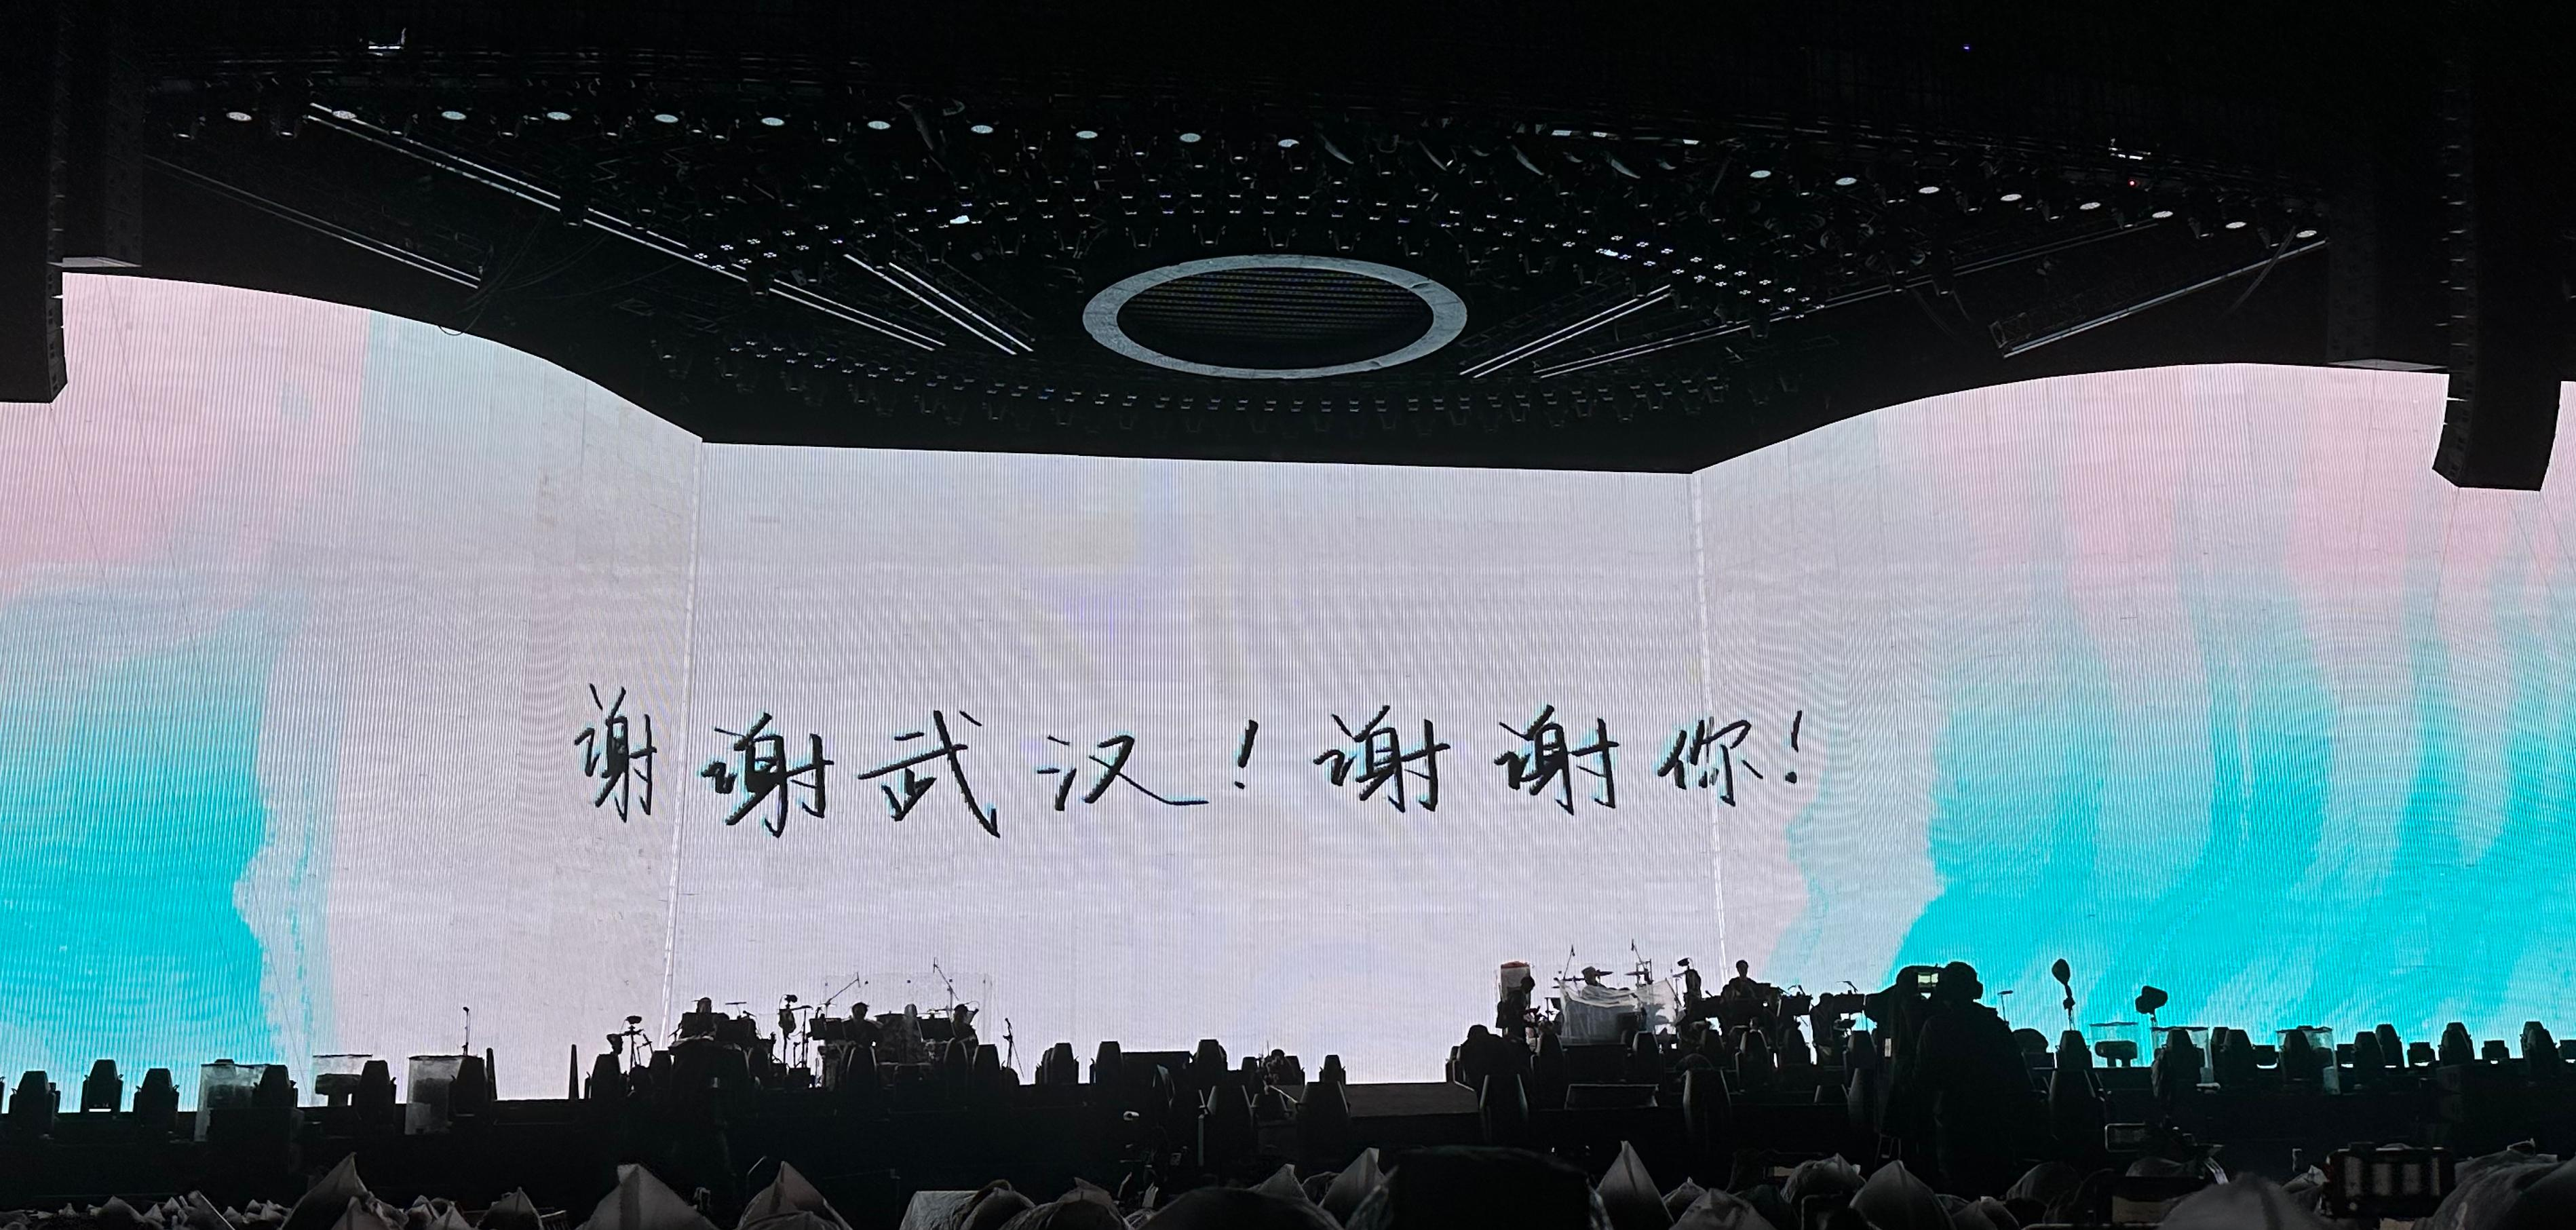
\includegraphics[width=400pt]{img/wuhan20240727/thank-wuhan} 

}

\caption{谢谢武汉!谢谢你!}\label{fig:unnamed-chunk-65}
\end{figure}

\hyperref[listen-to-me]{🎵【\textbf{听我说}】} 帮我唱好吗!(深:那个人总会懂得,那个人也可以是我\textasciitilde)

\hyperref[hope]{🎵【\textbf{望}】}\textbf{因为遇到你们,(深:我才心有所住。)}

  无论你们在任何地方都要记得只要你需要,我就在这里好吗!你从来不孤单。耶!

  然后现在感觉所有的无论是生活节奏还是怎么样,节奏非常非常快,所以压力非常非常大,就感觉很多人心中就会觉得,哎呀,我一定要怎么说,创造一个奇迹好像才非常厉害。但很多时候我想告诉大家,没事的,只要我们还在这条路上,我们就是那个奇迹,对不对?\textbf{不要害怕,因为当你出现的时候,他就已经是一个奇迹时刻!}

\hyperref[magic-moment]{🎵【\textbf{奇迹时刻}】}让我看到你们在,好不好?十周年快乐!(魔术师失误)没事,\textbf{奇迹时刻永远都有这么多例外,但是很精彩对不对!生米们生日快乐!!!}你们喜欢吗?(米:喜欢!)我尽力了(尬笑)但是我觉得只要给你们带来开心就好对不对!(米:对!)

  无论你是不是生米,你能不能跟我一起说一声祝生米(米:生日快乐!)如果刚好你今天生日,那我们也能祝你(米:生日快乐!)。总之无论你哪天生日我们都可以祝你(米:生日快乐!)。祝你天天开心!

\hyperref[happy-birthday]{🎵【生日祝福歌】}祝你生日快乐\textasciitilde 无论是哪天生日的人!我们都!祝你生日快乐\textasciitilde 来大声点哦!来的人就要天天开心,生日快乐!\textbf{我亲爱的生米!生日快乐!}

  谢谢老师们!而且诶先暂停,今天刚好也是我们音乐总监龙隆老师的生意(口糊)龙隆老师的生日!所以我们祝他(米:生日快乐!)。龙隆老师听到了吗?他的声音看来不够大。还是祝我们的生米(米:生日快乐!)。如果刚好你今天也生日,那我们也祝你(米:生日快乐!)。无论您哪天生日我们都祝你(米:生日快乐!)天天开心,谢谢你!谢谢谢谢!

\begin{figure}

{\centering 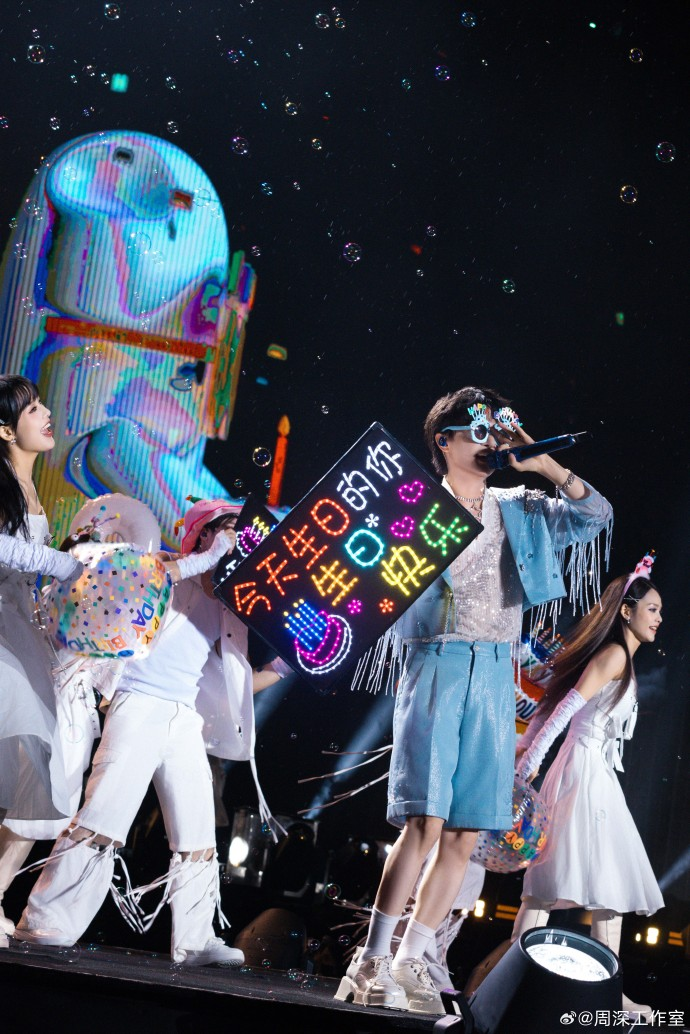
\includegraphics[width=400pt]{img/wuhan20240727/001} 

}

\caption{生日快乐 【@weibo-charlie-studio】}\label{fig:unnamed-chunk-66}
\end{figure}

  奥运会开始了,大家有看吗?最近有一个特别感人的瞬间,就是Steven Leo,他应该算是,就是在克服病魔在表演,我会觉得特别感动。然后很多时候看到很多他的片段我都会觉得在提醒我去珍惜每一次跟大家见面,在舞台上唱歌的瞬间,也再一次在我心中不停地翻涌出来。非常非常感谢你们能够听到我,让我慢慢慢慢去追逐自己的梦想,也希望你们能够跟我一起,也希望我能够永远陪着你们一起去追逐你们的梦想,好吗?里面有首歌叫非常非常好听,它叫应该是叫《love again》,它的意思就是说\textbf{你不用去创造非常多的奇迹,你只要不要停下你的脚步就可以。}你不用去做到任何就是一鸣惊人的事情,但是\textbf{你只要还在向前,迈的每一步都非常有意义。}无论现在你在什么阶段,你都可以成为自己最璀璨的冒险人。那么我也希望我们能够在这里祝我们的中国奥运健儿们能够精彩地绽放自己。中国奥运健儿(深\&米:加油!)。你们自己也加油!

\hyperref[adventurers]{🎵【\textbf{璀璨冒险人}】}

  向前冲好不好?谢谢谢谢谢谢。

【\textbf{点歌环节}】现在到了我们的点歌环节了。不要高兴太早,有没有可能,歌单你没有听过,但是我觉得这都是我心中非常宝贝的歌曲们,希望能够被更多人听到,好吗?我们会有9首歌曲,当我们的摄像机拍到指定一个人的时候,就要从这9首当中选一首出来,好不好?再一次非常感谢武汉场的每一个你!全场跟我倒数五个数字,123,5!4!3!2!1!您好在哪?在这?应应该是右边这个。不好意思。应该是欸,是哪个吗,应该,应该欸,哈哈哈,是我,对不起。对,应该是他,对不起,对不起。对,你们是一起的吗?哦是一起的。那我的心情就安分多了。应该怎么称呼您?(我叫小羽)小雨?是今天那个小雨吗?(米:不,是羽毛的羽)哦是第一套衣服的那个小羽。好,你多大呀?(米:14岁)。您旁边这位是,哦,那您的母亲该怎么称呼您?大羽?(小羽妈妈)你们是从哪里来的?重庆来的啊(重庆方言)。这里有没有其他从重庆来的?哦!真的有,谢谢你们,谢谢谢谢。那小羽同学,你是从几岁开始听我的歌的啊?(5岁)我怎么那么不相信。真的吗?(小羽:对,你大鱼就是发的时候我就开始听了)听了很久的大鱼,然后名字叫小羽。哈哈哈,也是一种很特殊的一个缘分。好,这些歌你都有听过吗?(米:听过)哦真的,哦哦啊哦欸哦,好吧,相信你,毕竟从5岁就开始听我唱歌了,谢谢你。那这9首当中有没有你想要听的歌!(米:三餐四季)。哦?哇塞,这么小众的歌,哇非常给我惊喜。谢谢谢谢,谢谢你。

  所以你刚开始听歌是妈妈给你听的,还是说你是无意间听到的还是怎么听到的?(米:我去看的那个电影)哦看了大鱼海棠哦。所以你还就是最后做到了大鱼海棠字幕的最后一行,然后听到了我的歌曲。非常感谢你,因为有一次我印象最深,我看大鱼海棠,然后在电影院,然后就一直在等自己的歌,等到了就是保洁工作人员在旁边,保洁工作人员跟我说,先生你好,没有彩蛋了。我说:``我知道没有彩蛋,但是后面是不是还有可能有一首歌?''哈哈哈,``好像是,应该是的吧?好像是叫那个什么周深唱的。''谢谢你,谢谢你,非常感谢,每一个瞬间让大家听到了我,谢谢小羽,也谢谢,怎么称呼你?除了生米妈妈。平时,好,谢谢您。愿意告诉我们怎么称呼您吗?(米:铁英。)铁英。好,谢谢铁英,谢谢小羽,谢谢!这一首三餐四季,希望大家喜欢。哇,完全没有想到,这是一首非常温暖的歌曲,也希望大家在外面拼搏的时候,或者是在任何地方拼搏的时候,都好好照顾好自己。

\hyperref[three-meals-a-day]{🎵【\textbf{三餐四季}】} 谢谢,好好照顾好自己。

  大家还想听吗?(米:想)谢谢你们还在,谢谢你们来,谢谢,\textbf{谢谢我们所有的相遇。}

\hyperref[keep-playing]{🎵【\textbf{不想睡}】}一起\textasciitilde 谢谢你。谢谢\textasciitilde 跟我一起(深、米:啦啦啦啦啦啦啦啦\ldots)再大声点,看台的\textasciitilde{}

  谢谢你们来,谢谢大家。我每一次都在不停的感慨,就是我们每一次的相遇有多么的不容易。就包括我们的导演,导演的老师们,他们也是就是改了非常多的航班和非常多的动车,因为天气原因,但是最终我觉得我们相遇了就是最好的事情。

  那我们也要掌声感谢我们非常多,让我们非常安全,非常开心一起相遇的人们,好不好?(米:好)感谢武汉的文化、公安、消防、交通等职能部门的大力支持,感谢我们场地支持武汉体育中心。感谢本次巡演的全程主办,北京时代立方文化传播有限公司,感谢演唱会制作单位必应,感谢我们的总导演周佑洋、庄惟惞。谢谢我们的音响总监金少刚,我再一次,每一次就非常想要,非常非常感谢金少刚老师。因为我们平时,我也不会经常去发微信或怎么样去打扰他,但是在我自己最需要的时候,然后金少刚老师,他愿意尽心尽力的去让我们更好的见面,让大家听到我的声音。大家觉得我的声音好听吗?(米:好听)都是要感谢金少刚老师,感谢我们今天的音乐总监龙隆老师。他也是今天的寿星,祝他(米:生日快乐)。感谢我们今天的乐队老师们,感谢我们的和声老师,感谢舞蹈老师们SDT ShowPro。好,谢谢大家,也要感谢我们的服装团队设计师劳伦斯许工作室,感谢时装品牌Windowsen。感谢我们的音响工程南京奥斯泰视听科技有限公司,感谢调音团队乐尔工作室,感谢硬体工程北京力超舞台集团。非常感谢每一个工作人员,大家知道吗?就是我们现在坐的这个凳子都是昨天我们老师们摆到五六点的,包括我们很多的志愿者们,我们谢谢他们,谢谢周深工作室,还是大家很激动的,是吧?感谢微博,感谢微博音乐,感谢微博演出,感谢现场所有的工作人员们。以及感谢来到武汉场的每一个你。刚才大家听的不想睡是卡布的晚安曲,周深也有一首他的晚安曲叫做(米:我以渺小爱你)。谢谢你们看到了我,也谢谢你们不嫌弃我渺小的力量去好好照顾你们,我们一定都会越来越好的,对不对?(米:对)我以渺小爱你,谢谢你。

\hyperref[loving-you-in-my-humble-way]{🎵【\textbf{我以渺小爱你}】}谢谢你们\textasciitilde{}\textbf{谢谢你们用这么汹涌、这么温暖的爱,来回报我渺小的这一份光,(深:我以短暂爱你不朽的旅程)我们一定会再相见的,再见。}

\section{Part5}\label{wuhan-20240727-part5}

\hyperref[the-wind-rises]{🎵【\textbf{起风了}】}谢谢你还在\textasciitilde!谢谢你\textasciitilde 以爱之名,你还愿意吗?(米:愿意)谢谢!

\hyperref[big-fish]{🎵【\textbf{大鱼}】}

  谢谢大家,谢谢大家,\textbf{完了,一起淋过雨的人,你就要记住我一辈子喽。}那我们来合照吧,我们先这边两张,然后这边一张,啊,直接湿掉,321,好,中间,321,今天我这条形码刘海还不错吧,哈哈哈,我都害怕扫我会扫出价格,哈哈哈。321,这边的朋友,你们好,那我们来这里。321,那边的朋友,休息会,哈哈哈,我又来啦,你们好。谢谢你们还在,看台的朋友们,321,谢谢大家。

  我还想耽误大家几分钟,听一下我新专辑的一首歌,好不好?(米:好)我有一首歌是三个字,它叫(米:少管我),没错,少管我,他听起来好像是一种争执或者是吵架,但是不是,他是一种自己对自己负责,自己知道最喜欢什么样的自己,对不对?(米:对)那又到了我们的少管我camera的时候啦。要学习我们嘿少管我的姿势,你们会吗?(米:会)谢谢,321,(深、米:嘿,少管我)。哇,你好棒哎,看台的朋友,321(深、米:嘿,少管我),这边的朋友321,(深、米:嘿,少管我),大家最大的声音,(深、米:嘿,少管我)。对嘛,这才是我们三点几万人的声音。那我们开始倒数5个数字喽,到时候抽到你的那个人,你的声音一定要喊的让大家都听见哦,5(米:4321)。zoom in zoom in zoom in,哦,是那个吗?应该是。对对,就是你就是你,哦,这里,哈哈哈。怎么称呼你?茶杯?不会是那两个字吧?哈哈哈,(米:宝贝)宝你们个头啊,怎么称呼怎么称呼?什么小盼?小焕?小麦?。小麦,小麦同学,你好,多少岁啊?是个秘密?哈哈哈,从哪里来啊?是个秘密?从哪里来?西安。武汉的小龙虾好好吃,特别好吃,特别好吃。好,那你准备好了吗?把所有不开心都可以喊开,我们大家全体安静要听你一个人的声音哦。小麦321,非常大声,谢谢你。

  让我们再来一个5,谢谢小麦,4321。你在哪里?哦,在这,好,怎么称呼你,奇怪的奇?石榴的石?为什么会迟疑了一下,然后点了头。是石,但是你说的不是石榴,对吧?你说是石头。哦,\textbf{那你以后要小心叫布的人哦},哈哈哈,好烂的梗。您从哪里来?厦门?那你是哪天到的这么厉害,今天早上到的?因为福建或者广东那边台风影响比较大。谢谢你来了,石先生,平时同事们也是叫您石先生吗?叫你石头的比较多,石头你好。宝你们个头啊。好,那你现在要用最大的声音,要比刚才我们小麦同学声音要大哦,你准备好了吗?哈哈哈,来,全场安静,321。你准备的很好,但是我没有准备突然被你骂的感觉。我们的手势是,嘿,少管我,他直接少管我。带上手势啊,右手,嘿,少管我好不好,来321。石头太优秀了我觉得,我觉得我们武汉的朋友们真的太棒了,有武汉本地的朋友不?武汉本地的朋友跟我来一句,嘿(米:少管我)。后面必须看台的同学跟我来一句,嘿(米:少管我)。我们全场的朋友跟我一起,嘿,(米:少管我),谢谢大家。

\hyperref[watch-ur-manners]{🎵【\textbf{少管我}】}\textbf{所有的烦恼,所有的不开心都会离我们远去的。}嘿,少管我,你就可以找到那个你最喜欢的自己。全场,(米:嘿!少管我!)你们太棒啦,又要来一次哦,54321(米:嘿!少管我!),全场,(米:嘿!少管我!)谢谢你们,全场再跟我大声喊,好不好?(米:好)54321,(米:嘿!少管我!)\textbf{你们是最棒的},这边,这边的朋友,54321,(米:嘿!少管我!)那边的朋友不能逊色哦,54321(米:嘿!少管我!)谢谢你们,**\textcolor{red}{我爱你们!}谢谢你们来,谢谢你们在,谢谢你们在任何时刻都陪着我,我也在任何时刻都希望能够陪伴着你,只要你需要,我都在这里,谢谢你们。全场再来一次,54321(米:嘿!少管我!)你们是最棒的。注意安全,东西不要掉了,不要生病啦,手机不要掉,证件不要掉,人身安全第一,任何时刻安全第一。谢谢,平平安安 的,全场54321(米:嘿!少管我!),谢谢武汉,安全第一,东西不要掉啦!

\begin{center}\rule{0.5\linewidth}{0.5pt}\end{center}

\begin{figure}
\centering
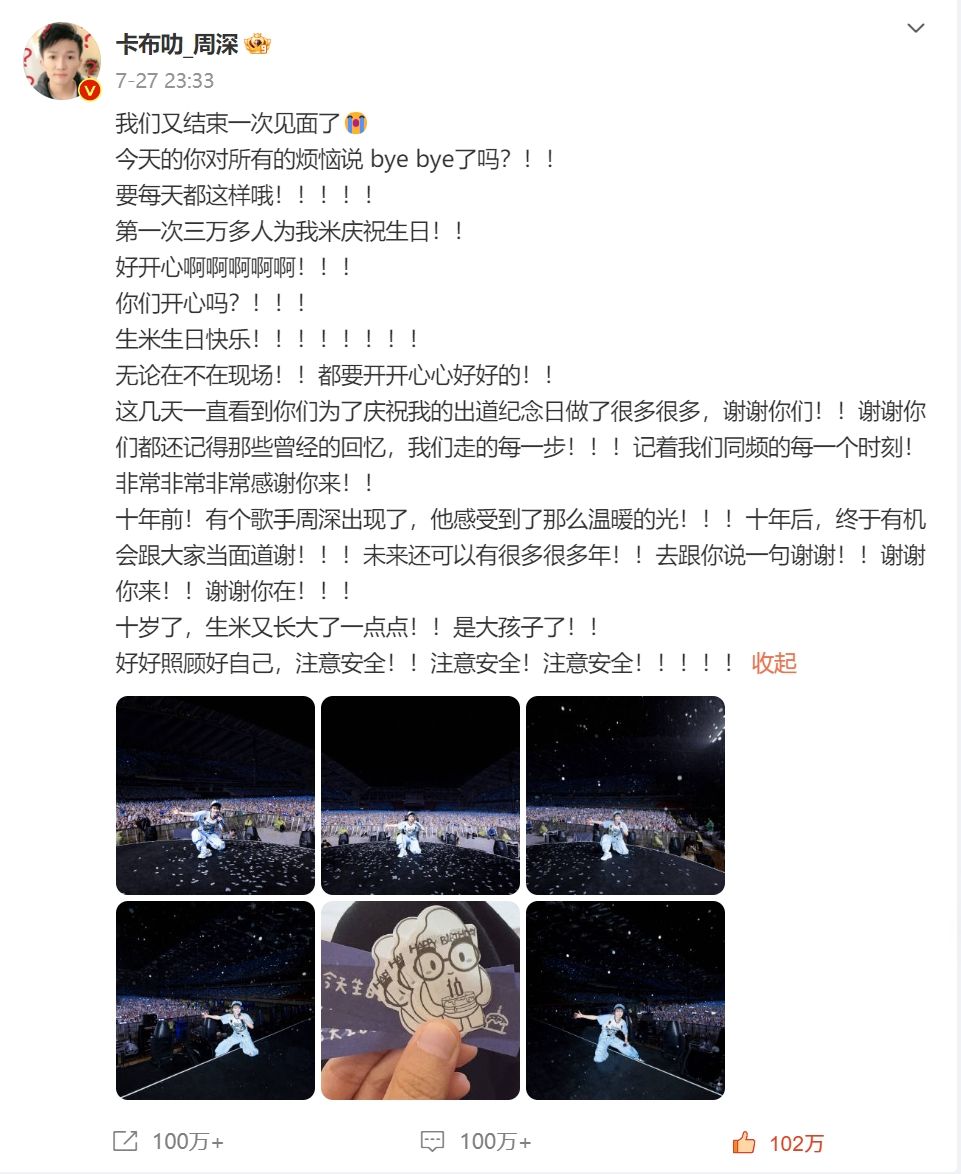
\includegraphics{img/weibo/wuhan-20240727.png}
\caption{\label{fig:unnamed-chunk-67}周深武汉体育中心主体育场演唱会结束微博 【\citet{weibo-charlie}】}
\end{figure}

\chapter{2024.08.10南京场}\label{nanjing-20240810}

\begin{quote}
\textbf{\emph{在这恍惚人间三万天当中,谢谢你愿意和我相遇。------ 周深}}
\end{quote}

\begin{figure}

{\centering 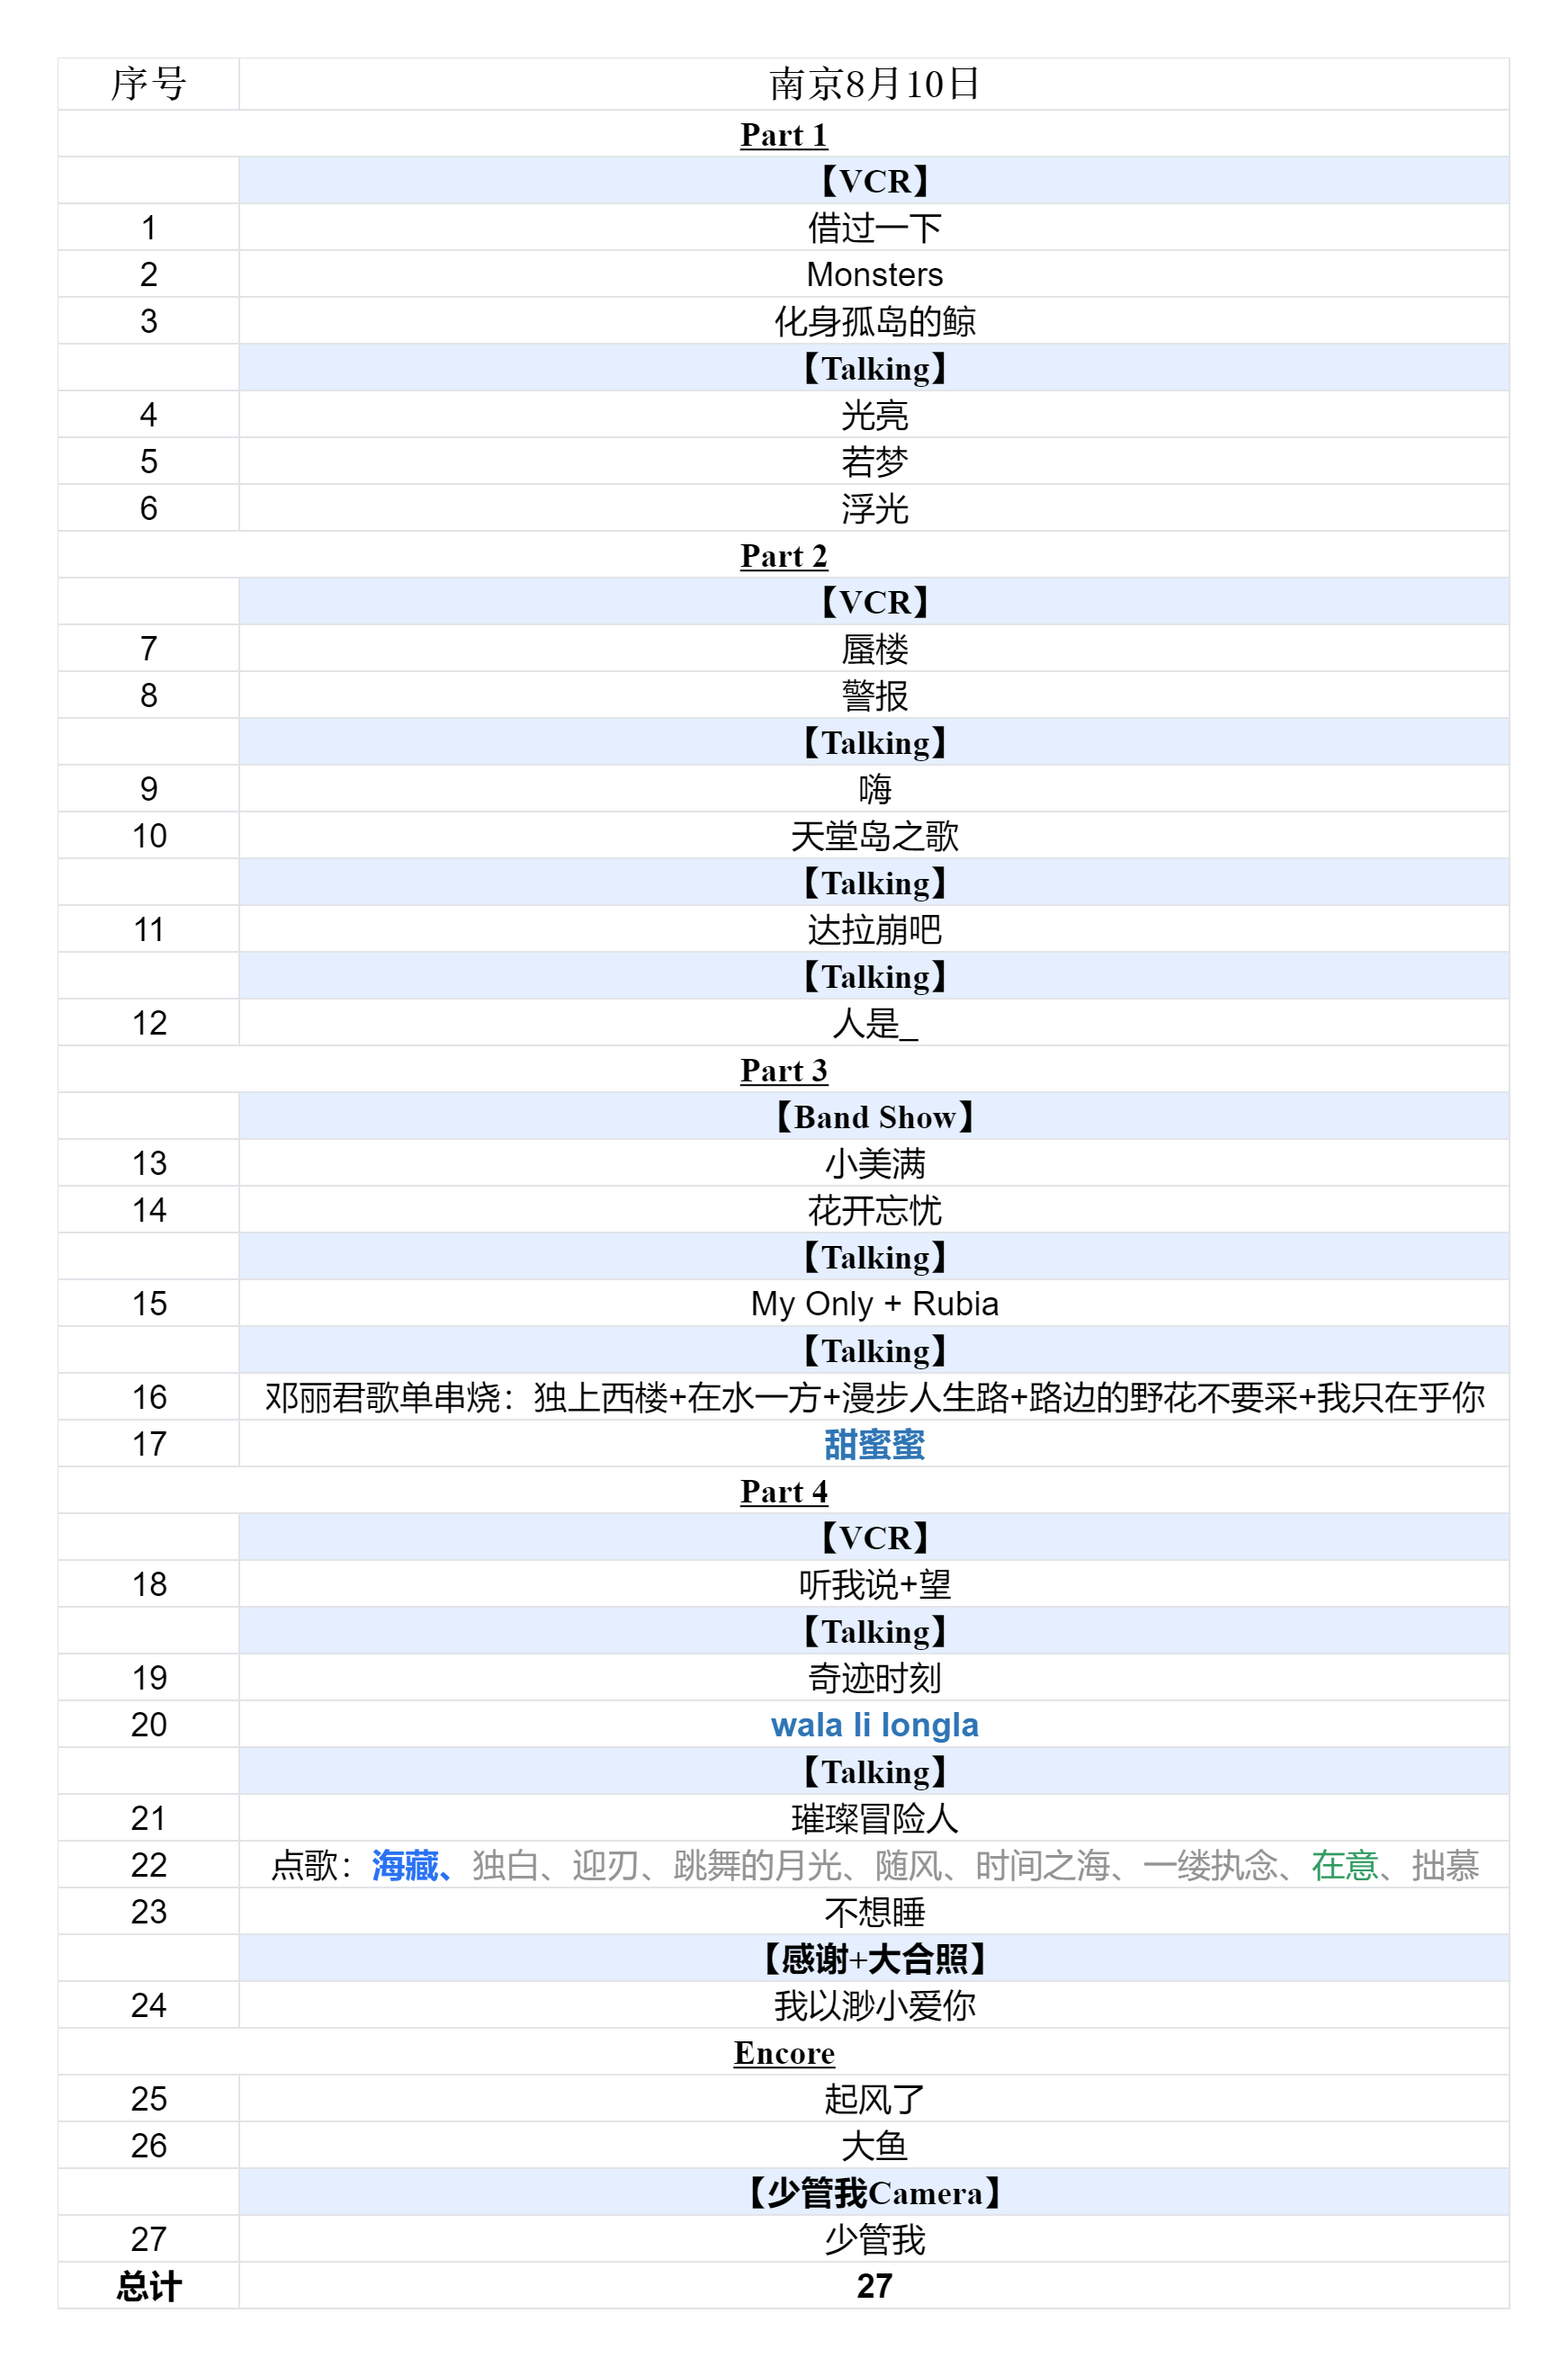
\includegraphics[width=320pt]{img/playlists/playlists-nanjing-20240810} 

}

\caption{2024周深9.29Hz巡回演唱会2024.08.11南京第一场歌单}\label{fig:unnamed-chunk-70}
\end{figure}

\newpage

\section{Part1}\label{nanjing-20240810-part1}

\hyperref[opening-vcr]{🎥【\textbf{开场VCR}】}

\hyperref[I-will-go-my-way]{🎵【\textbf{借过一下}】}南京的朋友们,你们好吗?(米:好)

\hyperref[Monsters]{🎵【\textbf{Monsters}】}

\hyperref[hua-shen-gu-dao-de-jing]{🎵【\textbf{化身孤岛的鲸}】}谢谢,大家好吗?(米:好)谢谢你们。这首歌愿意跟我一起唱吗?到你们\textasciitilde 看台的朋友\textasciitilde 你们太棒啦,到你们啦\textasciitilde 后面的\textasciitilde 一起\textasciitilde(米:没有墙头)特别浪漫,化身孤岛的蓝鲸来到了南京,南京的朋友们,你们好吗?(米:好)(深:无论你们有多少个墙头,你们也是我国王和王后)

  大家好,我是歌手周深,你们好吗?好。南京的畔西杆子们,你们吃了吗?哈哈哈,我看一下南京的畔西和杆子们在哪里?我说的很不标准,是吗?哈哈哈,意思是南京的美女们,帅哥们,你们好吗?(米:好)谢谢谢谢谢谢,非常开心能够来到这里跟大家相遇,然后接下来这首歌我非常喜欢,但是有一个小小的考题要考一下大家,请问莫听穿林(米:打叶声)下一句是?(米:何妨吟啸且徐行)哇,你们好棒啊,哈哈哈哈,没错,下一句就是何妨吟啸且徐行,希望大家不要就是考试的时候或者是背诗的时候记错这几句。如果真的记错了,因为听这首歌听太多,那就请去找制作人钱雷老师也是作曲人钱雷老师,和作词老师苟璘,以及加上苏轼,哈哈哈,\textbf{当然这首歌我觉得非常的有力量,也希望我们每个人都能够像伟大的文学家苏轼一样,无论是人生当中遇到什么样的狂风骤雨,都可以用乐观的心态去面对一切,因为一切都会好的,好吗?}(米:好)当我需要力量的时候,我发现哇,你们就是我的光亮\textasciitilde{}

\hyperref[silver-linings]{🎵【\textbf{光亮}】}后面的朋友,你们好吗?谢谢你们光亮了我,也希望你们(深:光亮你自己)

\hyperref[ruomeng]{🎵【\textbf{若梦}】}愿意给我听最好听的版本,你们的合唱吗?到你们了(米:往事流转,在你眼眸)后面的朋友\textasciitilde 你们太棒啦\textasciitilde 到这边喽(米:往事流转,在你眼眸)后面的朋友,(米:一边遗忘一边拼凑)这边(米:唯愿你能得到拯救)全场一起(深:往事)(米:往事流转在你眼眸)(深:在你眼眸)(米:一边遗忘一边拼凑)(深:拼凑)再大声点\textasciitilde 再来一遍(米:唯愿你能得到拯救)(深:因为你们,你你你你你你你,我才得到拯救)

\hyperref[floating-light]{🎵【\textbf{浮光}】}这首歌会跟我一起唱吗?(米:会)一起\textasciitilde{}\textbf{在这恍惚人间三万天当中,谢谢你愿意和我相遇\textasciitilde{}}

\section{Part2}\label{nanjing-20240810-part2}

\hyperref[senself-vcr]{🎥【\textbf{反深代词VCR}】}

\hyperref[mirage]{🎵【\textbf{蜃楼}】}

\hyperref[the-giver]{🎵【\textbf{警报}】}谢谢,谢谢我们舞蹈老师们\textasciitilde{}

  南京的朋友们,你们好吗?(米:好)终于感觉可以正式的打个招呼了,这边的朋友你们好吗哦?这边的朋友你们好吗?这边的朋友你们好吗?这一边的朋友你们好吗?那边看台的朋友你们好吗?哇哦,好,高楼上的朋友们,你们好吗?这边的朋友你们好吗?这一边的朋友你们好吗?哇塞,好多人。hello,我太开心了,而且非常非常感谢大家能够来跟我们相见,然后刚才我也很幸运的有时间去介绍了一个比较新的版本的周深,刚才演唱的歌曲是我新专辑(米:反深代词),没错,第一部分的时候是大家比较熟悉的周深,然后后面是比较不一样的周深,总之就是谢谢你们给我的安全感,让我能够愿意去把自己更全面或者更立体的自己给你们看,所以谢谢你们跟我相遇,谢谢你们。今天是什么日子呀?(米:七夕)错,今天是星期六。哈哈哈哈哈哈,我过了无数个星期六。哈哈哈,也过了个无数个不知道是星期几的七夕节,哈哈哈,但是没有想到,就七夕节对我来说也会非常有意义,因为在星期六的这天碰巧是七夕节,然后我跟大家见面啦!接下来这首歌是非常浪漫的一首歌,见面的时候就会说,\textbf{嗨,你好,嗨,新版本的周深,有一点温柔的周深来喽。你们会跟我一起唱吗?(米:会)}

\hyperref[say-hi]{🎵【\textbf{嗨}】}跟我一起\textasciitilde(深:谢谢是你啊)

\hyperref[haven-song]{🎵【\textbf{天堂岛之歌}】}谢谢老师们\textasciitilde{}

  今天是七夕节,也就是说一年一次的时候,牛郎和织女就会相遇,对不对?大家看,哦,我们看不到哦,但其实我觉得我们大家每个人的浪漫都特别的神奇,因为如果是牛郎星和流浪(嘴瓢),哈哈哈,牛郎星和织女星的话,他们中间其实相隔了十几公里,所以是非常远,但是因为我们他们就会一年相遇一次。然后其实\textbf{我认为我们每个人也都是在宇宙大爆炸当中形成的那个星辰,所以我们每个人都是星星,你们每个人都是发光的星星,但是我们在这里相遇了,那怎么能不说是一种极致浪漫呢?}谢谢你们,\textbf{\textcolor{red}{我爱你们~} }

  接下来这首歌它是一个童话故事,说的是谁拯救了谁,砍了谁,那谁又咬了谁,大家知道是什么故事吗?(米:达拉崩吧)但是最终他们还是过上了幸福美满的生活,所以我们也一定会过上幸福美满的生活的,对不对?那等一下你们愿意跟我一起说这个故事吗?(米:愿意)看台的朋友你们愿意跟我一起说这个故事吗?(米:愿意)我没听到,愿意吗?(米:愿意)巴拉蹦吧\textasciitilde{}

\hyperref[dalabengba]{🎵【\textbf{达拉崩吧}】}看台的朋友嗨起来,这边的朋友\textasciitilde 南京的朋友们准备好了吗?要到你们告诉我这个故事了,到底是谁救了谁?砍了谁?又咬了谁?最后这个故事是什么样的结局呢?上面的朋友,听好了,加速,最后\textasciitilde 王浩然的爸爸叫?达拉崩吧斑得贝迪卜多比鲁翁,对不对?(深:要念你来念吧)感谢大家,谢谢谢谢\textasciitilde{}

  刚才那首歌是?谁是听那首歌才认识我的?他是我在舞台,就是一个舞台啊,因为他不是我自己的歌,哈哈哈,然后我也非常幸运的是可以有很多舞台让大家去看到我,去认识我,去听到我,谢谢你们听到了我哦,谢谢你们哦。诶,他们说好像演唱会指哪里的话,哪里就会有非常热烈的欢呼声,是真的吗?那如果是这样呢?谢谢大家,感受到你们的热情,我非常非常开心,谢谢大家,也希望大家多多注意安全。那我也很开心的是可以在很多电影和电视剧当中去被大家听到,接下来要演唱的是流浪地球2的人是\_。\textbf{在七夕这么浪漫的日子当中,想想我们要带着地球一起去流浪,带着地球走,这怎么能不说是一种极致浪漫呢?但是我发现任何浪漫都不如我们相遇了这件事更浪漫,对不对?}(米:对)希望你们喜欢人是\_

\hyperref[renshi]{🎵【\textbf{人是\_}】}谢谢\textasciitilde{}

\section{Part3}\label{nanjing-20240810-part3}

\hyperref[happy-ending]{🎵【\textbf{小美满}】}你们愿意跟我一起唱吗?(米:愿意)这首歌就交给你们喽,后面的朋友们,要大声唱哦\textasciitilde 谢谢你们,遇见你们是我最大的小美满\textasciitilde 到这边喽\textasciitilde 后面的\textasciitilde 我们全部一起\textasciitilde 谢谢你们,南京的朋友们,你们好,我是歌手周深,你们好吗?(米:好)小美满这首歌是每次我一听我就觉得非常的美好,所有愿望都可以实现的一首歌,所以我们不妨在这首歌当中许个愿,好吗?(米:好)等一下,要怎么说呢?大家要听我的话,我数,叫大家闭眼的时候,大家一定要闭眼睛,默默许一个愿望,像我这样,闭眼睛,想好心中的愿望,321,我喊睁眼的时候,当当,愿望就会在这棵树上,所以大家现在闭上眼睛,无论你是什么工作,什么年龄段的,现在闭上眼睛,默默许下一个愿望。想想你想许什么愿望呢?但是这个愿望有一个要求,就是必须是关于自己的愿望。你有多久没有问过一下自己好不好啦?辛苦自己啦,也谢谢自己把自己照顾得这么好,321\textasciitilde 你的愿望一定会被提听见的,谢谢你们\textasciitilde{}

\hyperref[no-worries]{🎵【\textbf{花开忘忧}】}宝你个头,七夕也是会宝你的头的\textasciitilde(深:我会说)(米:你好啊)hi,你好啊\textasciitilde 我来你家看你啦\textasciitilde 我们一起好吗?(深、米:我们苍老的时候\textasciitilde)花开忘忧,愿你无忧,花开忘忧,(米:愿你无忧)离开的人一定会听见的,对吗?(米:对)

  宝你个头啊,谢谢\textasciitilde 在这个非常浪漫的日子呢,我有给大家准备一颗糖,你们有收到吗?希望大家在成为更好的自己的路上,我们一定会有更高的目标,对自己会越来越,可以说是苛责,不停的在向,希望自己可以变得更好,\textbf{但任何时候希望大家都不要忘记一颗糖就可以拥有的快乐},好吗?(米:好)也希望这个儿时的一个回忆,当然有可能你现在正在是儿时,哈哈哈,也可以永远让这一份甜记得很久很久,你需要的时候就去把这份回忆拿出来,好吗?(米:好)我很幸福,我也有这样一份回忆,是你们给我的,我找遍了世间所有最甜的糖,我都发现,没有你们甜诶\textasciitilde 说这么多话是因为等下又要弹钢琴,哈哈,我也一把年纪,老大不小了,哈哈,等一下你们会用爱来鼓励我吗?(米:会)但是,等一下要弹的歌曲我自己是非常喜欢的,我觉得它永远在很多时刻出现的时候都会伴随着温暖。你们会喜欢这样的歌吗?(米:会)也希望你知道从任何时候开始学一件自己喜欢的事情都不会玩哦\textasciitilde{}

\hyperref[my-only]{🎵【\textbf{My Only}】}

\hyperref[rubia]{🎵【\textbf{Rubia}】}星期六快乐,七夕快乐,天天都要开心哦\textasciitilde 汗水真的好咸啊\textasciitilde 谢谢,谢谢,无论任何时刻,他都让我好像回到家一样,谢谢你们。

  \textbf{刚才我有说我们每个人其实都是在宇宙大爆炸的时候降落的一颗星辰,我们都是一颗美丽的星星},大家还记得吗?要说到,(深换外套,米尖叫)你们不要每次我在脱外套的时候尖叫声那么大,我会觉得我不用唱歌,哈哈哈。要说到一直在给我指引方向,去唱歌方向的一颗星星,一定要说的是就是邓丽君女士,她的歌你们听过吗?(米:听过)你们喜欢听吗?(米:喜欢)她一直在鼓舞我去好好的,她的歌声,她的音乐一直鼓舞我去好好的,如何成为一个自己喜欢的歌手?就是不停的唱歌,我也希望自己以后能够有很多歌曲,隔了好多年,好多年之后,大家还记得每首歌里面都可以存着大家很多很多美好的时光,能够成为大家存放记忆的地方,好吗?(米:好)我一定会继续好好唱歌的,前面的朋友你们听到了吗?那边的呢?那等一下如果你会唱的话跟我一起唱哦(米:好)我还没有唱,那边要传来一个好听,哈哈哈哈,(米:好听)你们唱的好不好听啊?(米:好听)好听那你们上来唱,哈哈哈,希望你们能够喜欢,记得跟我一起唱\textasciitilde{}

🎵【\textbf{邓丽君组曲}】(米:路边的野花你不要采)你们这么多墙头还这么说(米:没有)你们会记得我吗?(米:会)谢谢,\textbf{全世界最甜的生米,最甜的你。}

\hyperref[sweet]{🎵【\textbf{甜蜜蜜}】}(深:啊,在谁的微博里,微博里你的ID如此熟悉)谢谢你们,今天是七夕,无论你已经找到了那个,怎么说,一起奋斗的人,那祝你们甜甜蜜蜜,如果没有的话,也可以像我一样好好的照顾好自己,对不对?(米:对)宝你个头啊这位朋友,到你们(米:甜蜜笑得多甜蜜)谁最甜?(深:是你,是你,梦见的就是你)谢谢你们给我创造的无数美梦\textasciitilde{}

\newpage

\section{Part4}\label{nanjing-20240810-part4}

\hyperref[thank-you-vcr]{🎥【\textbf{谢谢南京,谢谢你VCR}】}

\begin{figure}

{\centering 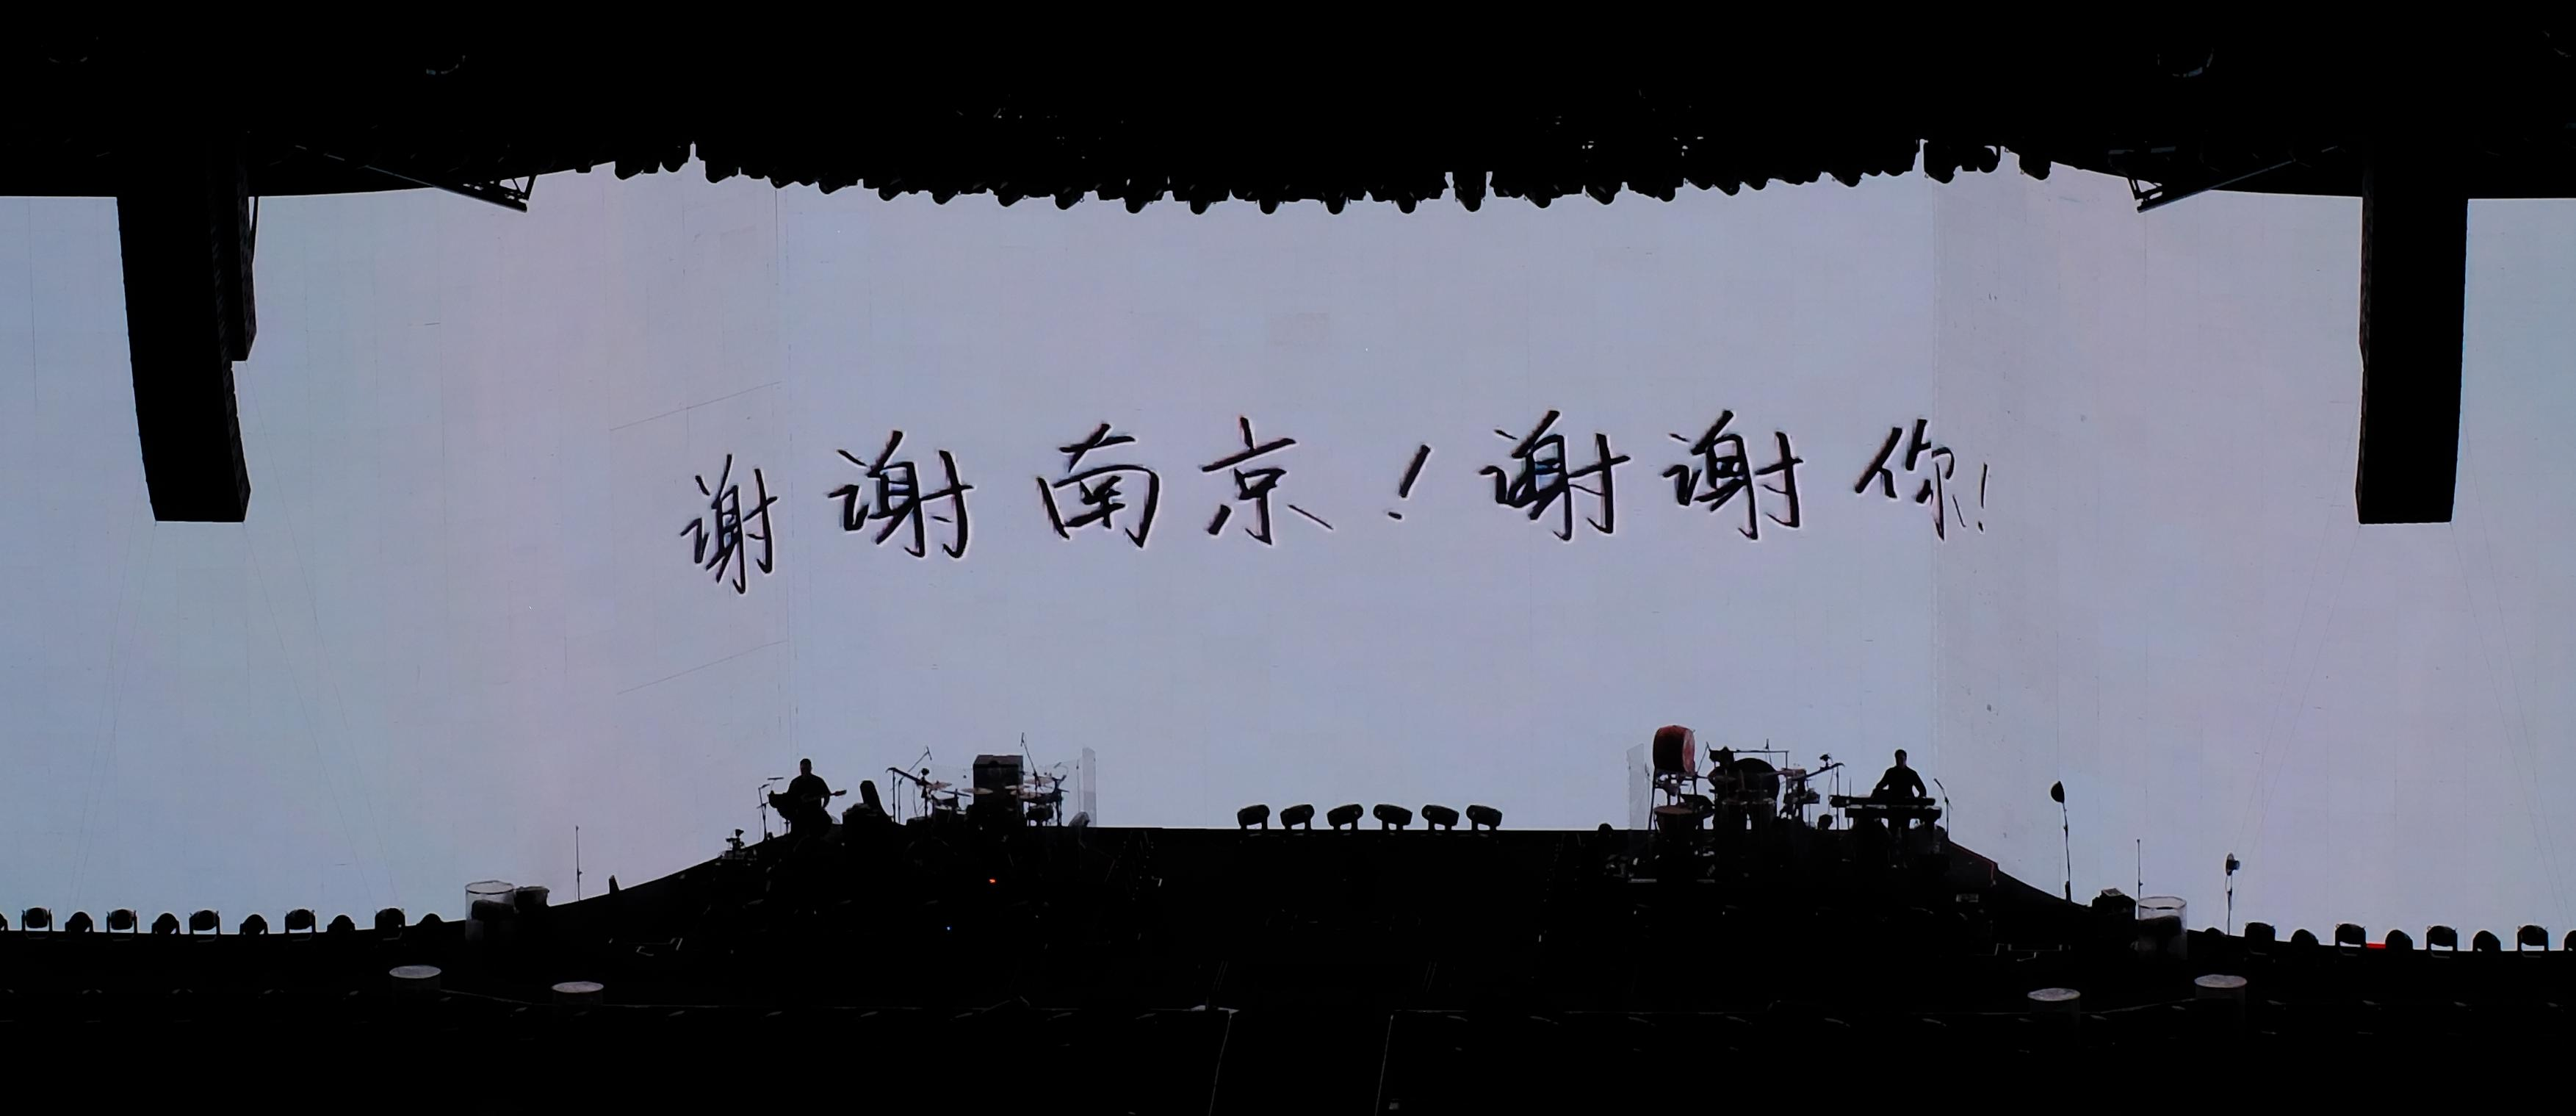
\includegraphics[width=400pt]{img/nanjing20240810/thank-nanjing} 

}

\caption{谢谢南京!谢谢你!}\label{fig:unnamed-chunk-71}
\end{figure}

\hyperref[listen-to-me]{🎵【\textbf{听我说}】} \hyperref[hope]{🎵【\textbf{望}】}听我说,我也想听你们说,跟我一起,好吗?(米:好)我听你们说(米:听我说,可以听我说)那个人也可以是我\textasciitilde 到你们\textasciitilde 到你们,(米:我们总会绕啊绕)看台的朋友\textasciitilde 因为每一个你,每一个你哦(深:我才心有所住)祝我们七夕快乐\textasciitilde{}

  大家平时玩游戏吗?怎么有人提前开笑?有人,你们打的好吗?看台的朋友,最高的那位朋友,你玩的好吗?好,听不见,哈哈哈,我一般不是很厉害,但是我觉得,无论是输还是赢,在游戏里都可以找到快乐,而且输着输着说不定就迎来了自己的奇迹时刻,你们说对不对?所以任何时候不要害怕输,不要害怕任何东西,我们继续尝试,我们继续向前,我们继续找寻自己。你就会为自己创造那一个奇迹时刻。结果切的完全不是这一机位\textasciitilde{}

\hyperref[magic-moment]{🎵【\textbf{奇迹时刻}】}大家好,七夕的时候我给大家写了一封信,信上面写的是什么呢?七夕快乐,星期六也快乐哦。现在我要把这个信放在这个信托当中,我需要全场跟我喊321,来,321,我的心愿都能化作千纸鹤走到你身边。接下来我还给大家准备了一束花,但是只要你们让我感受到爱,我们全场倒数321,321,这一束花我送给你了\textasciitilde{}

\begin{figure}

{\centering 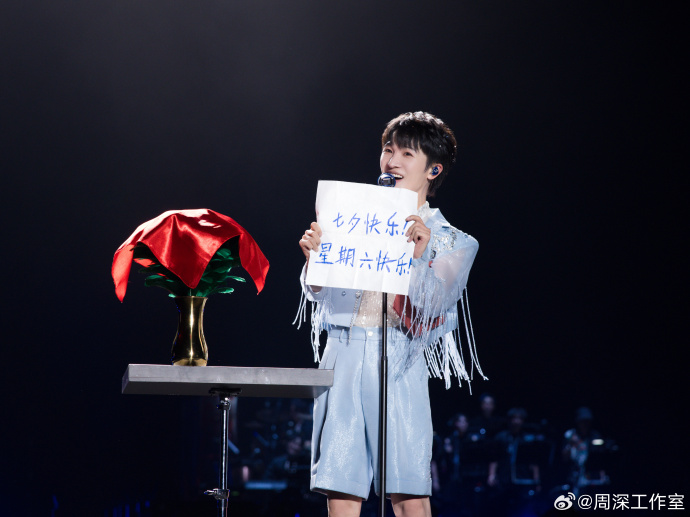
\includegraphics[width=400pt]{img/nanjing20240810/001} 

}

\caption{七夕快乐 【@weibo-charlie-studio】}\label{fig:unnamed-chunk-72}
\end{figure}

  我的魔术是不是进步了?哎呀,大家听到这首歌什么歌吗?大家等一下要一起跟我来哦,好不好?好,那我们的音乐全部也重新来一下吧,哈哈哈,我们先预习一下,我们有个快乐的密码叫做,(米:wala li longla)我们试一下wala li longla,这边,wala li longla。只要念出这个密码,所有的事情都会清除他的沟通成本,所有事情都变得非常的简单,所有的事情都变得非常的快乐。我们全场再来一遍(米:wala li longla)谢谢\textasciitilde{}

\hyperref[wala-li-longla]{🎵【\textbf{wala li longla}】}全场朋友们愿意跟我一起念这个快乐吗?(米:愿意)那等下跟着我哟,一定好好配合我哦,321,wala,wala li,wala li long,wala li longla,再来,wala,wala li,wala li long,wala li longla\textasciitilde 这里充满着最多最多的快乐,再跟我一起唱两句好吗?aho,唱(米:aho)aho,唱\textasciitilde 再来\textasciitilde 看台的朋友\textasciitilde 全场\textasciitilde{}

  好想再感受一次,54321(米:wala li longla)好快乐,wala li longla,谢谢,谢谢谢谢,希望你永远快乐的,永远照顾好自己,一路向前冲,你终将会收获属于你的璀璨。各位璀璨冒险人们,出发吧。

\hyperref[adventurers]{🎵【\textbf{璀璨冒险人}】}到你们\textasciitilde{}\textbf{\textcolor{red}{我爱你们~} } 到你们\textasciitilde(米:还想要继续吗)要(米:要逆风不退啊)璀璨冒险人们,向前出发吧,好吗?

  谢谢,谢谢大家,谢谢大家,你们听着好听吗?(米:好听)今天大家来开心吗?(米:开心)有没有好好的照顾好自己?(米:有)看台的朋友呢?

【\textbf{点歌环节}】
那又到了我们点歌时间哇,不要高兴的太早,因为那首歌可能你没有听过,哈哈哈,他都是我相对来说比较宝藏一点的歌单,但是我相信他一定也是某一个人心中最喜欢的那首歌,对不对?(米:对)好,那我们等一下,全场倒数五个数字我们就直接找到他,好不好?(米:好)来,我们摄像老师先整个转起来,我有点晕,哈哈,来,全场5,(米:4321)停,哇,你好你好你好,你在哪里?(在这里)在这里哇,老师,给他一点点光。哇,你今天好漂亮啊。(谢谢)谢谢你,谢谢(专门做来见你的),谢谢谢谢谢谢,谢谢,也希望你以后想要这么漂亮的时候随时都可以,好吗?(好的)谢谢谢谢,我有看到很多其他很漂亮很帅气的你们,谢谢你们,你是哪里人呀?(我是上海来的)上海来的,会不会上海话?(一点点),但是朋友我们在南京,(南京话不会)我会一句,南京的攀西杆子们,哈哈哈,是这样说吗?不是这样说是吗?全场沉默了,哈哈哈,我回去要找一下我那个南京朋友练一下,怎么称呼你,(叫我糯米吧)糯米,好,来自上海的糯米朋友,你好,辛苦你了。你什么时候开始听我唱歌的?(我初二,14年的时候)14年的时候?(对的)您才初二,哈哈哈,是的,14年,也就是我出道的时候了。您初二的时候我出道了,哈哈哈,那非常,那听我的歌有大概哦,十年了。(对,正好十年)听我的第一首歌是?(该说不说是欢颜)这里有其他人听过我的欢颜吗?应该说听过我的舞台欢颜吗?是齐豫老师的一首(深:只要你轻轻一笑)哇,不该晾着你,对不起,哈哈哈,(没事没事没事)第一首歌是欢颜,那第二首歌是什么歌?(第二首是大鱼)第三首?(化作孤岛的鲸),记错了,化身孤岛,(化身孤岛的鲸,对不起,我给你跪下)不会,这首歌特别奇妙,因为在南京,我们唱化身孤岛的蓝鲸。谢谢您,那今天你看一下这9首歌当中你想听哪一首?(6号海藏)有这么多人喜欢海藏吗?这边的朋友喜欢吗?你为什么会选这首歌?(我从深圳开始就想点这首歌了)哇塞,谢谢你,谢谢,辛苦了辛苦了。谢谢,谢谢,谢谢。希望你在支持我之前先照顾好自己,好不好?(可以最后再说一句吗?)你要说什么?(深深嫁给我)侬想得美,开玩笑了,谢谢你,谢谢糯米\textasciitilde 那这首海藏希望你们喜欢,也希望你们归来依然是那个初心不忘的少年\textasciitilde{}

\hyperref[ocean-treasure]{🎵【\textbf{海藏}】} 谢谢南京的朋友们,好听吗?(米:好听)

  谢谢你们让一个普普通通的男孩子慢慢去靠近他的梦想,你们也一定可以的,加油,好吗?(米:好)周深可以,你也一定可以\textasciitilde{}

\hyperref[keep-playing]{🎵【\textbf{不想睡}】}谢谢你们看见了我\textasciitilde 到你们\textasciitilde 到你们\textasciitilde 这边的朋友\textasciitilde 看台的朋友\textasciitilde 那边的朋友\textasciitilde 谢谢你们\textasciitilde 一起\textasciitilde 看台的\textasciitilde 后面的朋友\textasciitilde 这边\textasciitilde 太浪漫啦\textasciitilde{}

  谢谢,我刚才一睁眼看到那么多星星的时候特别感动,同时我也非常的担心,手机应该不会发烫到关机哦。好,大家先保护一下自己的手机,可以先收一下,哈哈哈,但是非常非常漂亮,谢谢你们。还有就是我有看到一个非常浪漫的说法,就是说宇宙非常非常大,我们也许在此时此刻我们点亮那个手电筒,我们散发出去的那个光子,在多年之后它依然会在宇宙的另外一端相遇,也就是说,\textbf{也许多年之后宇宙当中还会漂浮着我们这一段浪漫的光点。我们赢麻了}。

  当然我们也非常开心,也非常感谢很多很多工作人员对我们这一次相遇的支持,对不对?(米:对)我们感谢场地支持南京奥体中心,感谢我们全程主办北京时代立方文化传播有限公司。感谢南京承办方,江苏中奥国际体育文化传媒有限公司。感谢我们演唱会制作单位必应。感谢我们演唱会的总导演周佑洋、庄惟惞。谢谢我们的音响总监金少刚,谢谢我们的音乐总监龙隆老师。感谢我们今天的乐队老师们,以及我们的和声老师们。感谢我们的舞蹈团队SDT ShowPro,谢谢你们,辛苦了啊。谢谢服装团队设计师劳伦斯许工作室,感谢时装品牌Windowsen,谢谢音响工程,南京奥斯泰视听科技有限公司,谢谢调音团队乐尔工作室,谢谢我们的硬体工程北京力超舞台集团。谢谢经纪公司周深工作室的小伙伴们,(米尖叫)糟糕了,在七夕的时候小小的吃了一下醋,谢谢周深,(米狂叫)不会不会,谢谢你们,真的很感谢我们工作室的小伙伴,就很多,我要去表达的话,去做的事,他们都帮我们去,慢慢去跟我们的米子们听到了,要好好照顾自己哦。有没有?看台的朋友有没有?感谢微博?(米:倒闭)感谢微博音乐(米:倒闭)感谢,哈哈哈,我不感了,感谢微博演出(米:倒闭)。当然,我们要感谢南京,谢谢南京这座城市,以及感谢南京所有职能部门的大力支持。当然最最最最最最重要的也是每一个来到南京现场跟我们相遇的你,谢谢你,也谢谢我们南京台前幕后所有的工作人员们,谢谢大家,大家要好好照顾好自己哦,(米:好)谢谢你们。

  我们合照吧,辛苦老师开下场灯。哦,hello,哇塞,你们好漂亮好帅气啊,谢谢,谢谢,谢谢,hello,hello,哇塞,大哥你好冷漠,哈哈,开玩笑的,完了完了,我让他尴尬了,哈哈哈,我们来合照吧,这边的朋友,哈哈哈,糟糕,要内耗了,哈哈哈,321。好的,来我们这边的朋友,321,我们中间的朋友,来,321。当然也少不了我们那边的朋友啦。哈哈哈,我来啦,哈喽,你们好,双眼皮掉了,双眼皮掉了,没事,好,来,这边哦,这边,321,迅速迅速,好,321,哇塞,南京的舞台好大呀。那边的朋友你们好吗?(米:好)(深深跑去另外一边舞台,米:加油加油加油)321,321,谢谢大家,我今天肯定又刷新了我的步数了。嗓子也太好了吧,刚才演唱的不想睡是卡布的晚安曲,周深也有一首晚安曲,叫做(米:我以渺小爱你)我以渺小爱你。

\hyperref[loving-you-in-my-humble-way]{🎵【\textbf{我以渺小爱你}】}不要嫌弃我的力量不够大好吗?谢谢你们,\textbf{\textcolor{red}{我爱你们} },谢谢你们看到了渺小的我\textasciitilde 我也不知道我还能够在舞台上唱多少年,但是谢谢你们,(深:我以短暂爱你不朽的旅程)谢谢大家\textasciitilde 大家辛苦了,谢谢你们,看台的朋友,谢谢\textasciitilde{}

\section{Part5}\label{nanjing-20240810-part5}

\hyperref[the-wind-rises]{🎵【\textbf{起风了}】}谢谢\textasciitilde 以爱之名,你们还愿意吗?(米:愿意)

\hyperref[big-fish]{🎵【\textbf{大鱼}】}

  谢谢你,谢谢你们,谢谢你们愿意跟我相遇,然后可能还要再耽误一下大家一点时间,因为还有一首专辑里的新歌想让大家听一下,好吗?谢谢你们,很开心很开心,你们愿意继续等着听歌。然后也谢谢你们来,谢谢你们一直在,谢谢你们。那在唱这首歌之前,我们有一个小小的环节叫做,(少管我 cam camera)没错,少管我 cam,camera,少管我,他其实是一个需要足够安全感才能够说出来的三个字,很多时候大家会误解为它是争执,但其实更多时候它是一种安全感,回应那个安全感,告诉他我知道怎么去寻找那个最好的自己,也谢谢你们给我这一份安全感,让我居然敢说出这三个字,谢谢你们。当然也不要误解这三个字,这三个字代表的是对自己负责。

  那我们话不多说,倒数5个数字,如果这个摄像机拍到你的话,你就要用全身最大的力气喊出最大的声音,喊出少管我三个字好不好?但是有一个固定手势,就是,嘿,少管我,但是要注意不要敲到前面人的脑壳。哈哈哈,好,全场倒数5个数字,5(米:4321)停,这位先生,你在哪里?您这么腼腆的姿势我怕是找不到你,啊在这是么?hello,你好,您叫什么?怎么称呼您?啊?鱼?宜?啊啊,木子李,大家欢迎李先生,您从哪来?从哪儿?宣城,哦,哈喽,你好,您方便问多大吗?这样吧,不方便啊?哈哈哈,这也很好,我们也要保护好我们的年龄,所以以后不要到处在外面说我已经31岁了,那您听我的歌多少年呢?四年哦,那算,那也挺久的,你们能够一直听别人的歌听四年,而且愿意来演听演唱会。谢谢你,谢谢李先生。对,然后那你愿意跟我们一起喊出这一句,试试嘛?旁边的是他的朋友吗?是朋友,那他为什么一副我根本不认识,哈哈哈,你们俩一起来的?哦,好的,来吧,你为什么喊这句话之前看向的是旁边的她,方便说一下,你两二位是?(猫猫吃瓜,深:甜蜜蜜,你笑得甜蜜蜜),平时在家里都听谁的呀?开玩笑,那这位女士怎么称呼?唯?唯?唯?微唯尾?微唯尾女士你好,那第三声尾?第二声唯?啊唯女士您好,那我希望您可以转向您的右边,然后看我们李先生大声喊出这句,嘿,少管我。哈哈哈哈,灯光老师给他光,把他照得最亮,哈哈哈,李先生在说,啊,怎么办?来,来我给你复习一下,嘿,少管我,(李先生冲着他老婆嘿,少管我)我不是这个意思,没让您冲着她喊,您冲着我喊,她看着您,再来321走。哈哈哈,掌声给李先生。

  我们再来抽一位朋友来,全场倒数5个数字,谢谢李先生,谢谢唯女士。5(米:4321)停,他在哪里?在这边吗?在这边这边?好。怎么称呼你?小蒋?小贾还是小蒋?蒋,小蒋,好,蒋女士,你好,您大概是从什么时候开始听我的歌呢?19年?哦,听到的第一首歌是?追是吗?Monster,哦,我当时也是因为在我们的歌里面翻唱了这一个片段,发现,诶,很多人喜欢,所以后面在歌手当打之年的时候唱了一下,所以刚才您还喜欢我唱这个版本吗?那我可以听您唱一下吗?哈哈哈,话筒给你的话呢?哈哈哈,好的,蒋女士来,大声喊出,嘿,少管我,所有的不开心,所有的烦恼都会离你远去,好不好?好321,谢谢,我觉得稍微不够大声,大家再给她一点鼓励。321,芜\textasciitilde 那我们全场的朋友跟我来一遍好不好?321,(米:嘿,少管我)希望所有的不开心,所有的烦恼全都离你远去,而那个你最喜欢的自己,向你越靠越近,七夕快乐\textasciitilde{}

\hyperref[watch-ur-manners]{🎵【\textbf{少管我}】}掌声欢迎我们舞蹈老师们\textasciitilde 来喽\textasciitilde 全场最大的声音,54321\textasciitilde 全场,54321\textasciitilde 全场\textasciitilde 谢谢你们,54321,(米:嘿,少管我)\textbf{\textcolor{red}{我爱你们} },七夕快乐,谢谢你们来,好好照顾好自己好吗?好好的开心的继续去寻找那个你自己最喜欢的自己,好吗?所有的烦恼途通通离我们远去,54321,你们是最棒的,爱你们!谢谢你们,54321(米:嘿,少管我)你们太棒了,543212\textasciitilde54321\textasciitilde 谢谢你们,大家注意安全,手机不要掉了,证件不要掉了,平平安安到家好吗?(米:好)看台的朋友听到了吗?前面的朋友听到了吗?希望你们健健康康,平平安安。谢谢你们来相遇,希望我们相遇不只是七夕,而是每一个朝夕。注意安全,谢谢\textasciitilde{}

\chapter{2024.08.11南京场}\label{nanjing-20240811}

\begin{quote}
\textbf{\emph{感受这一份快乐吧,我最爱的你们。------ 周深}}
\end{quote}

\begin{figure}

{\centering 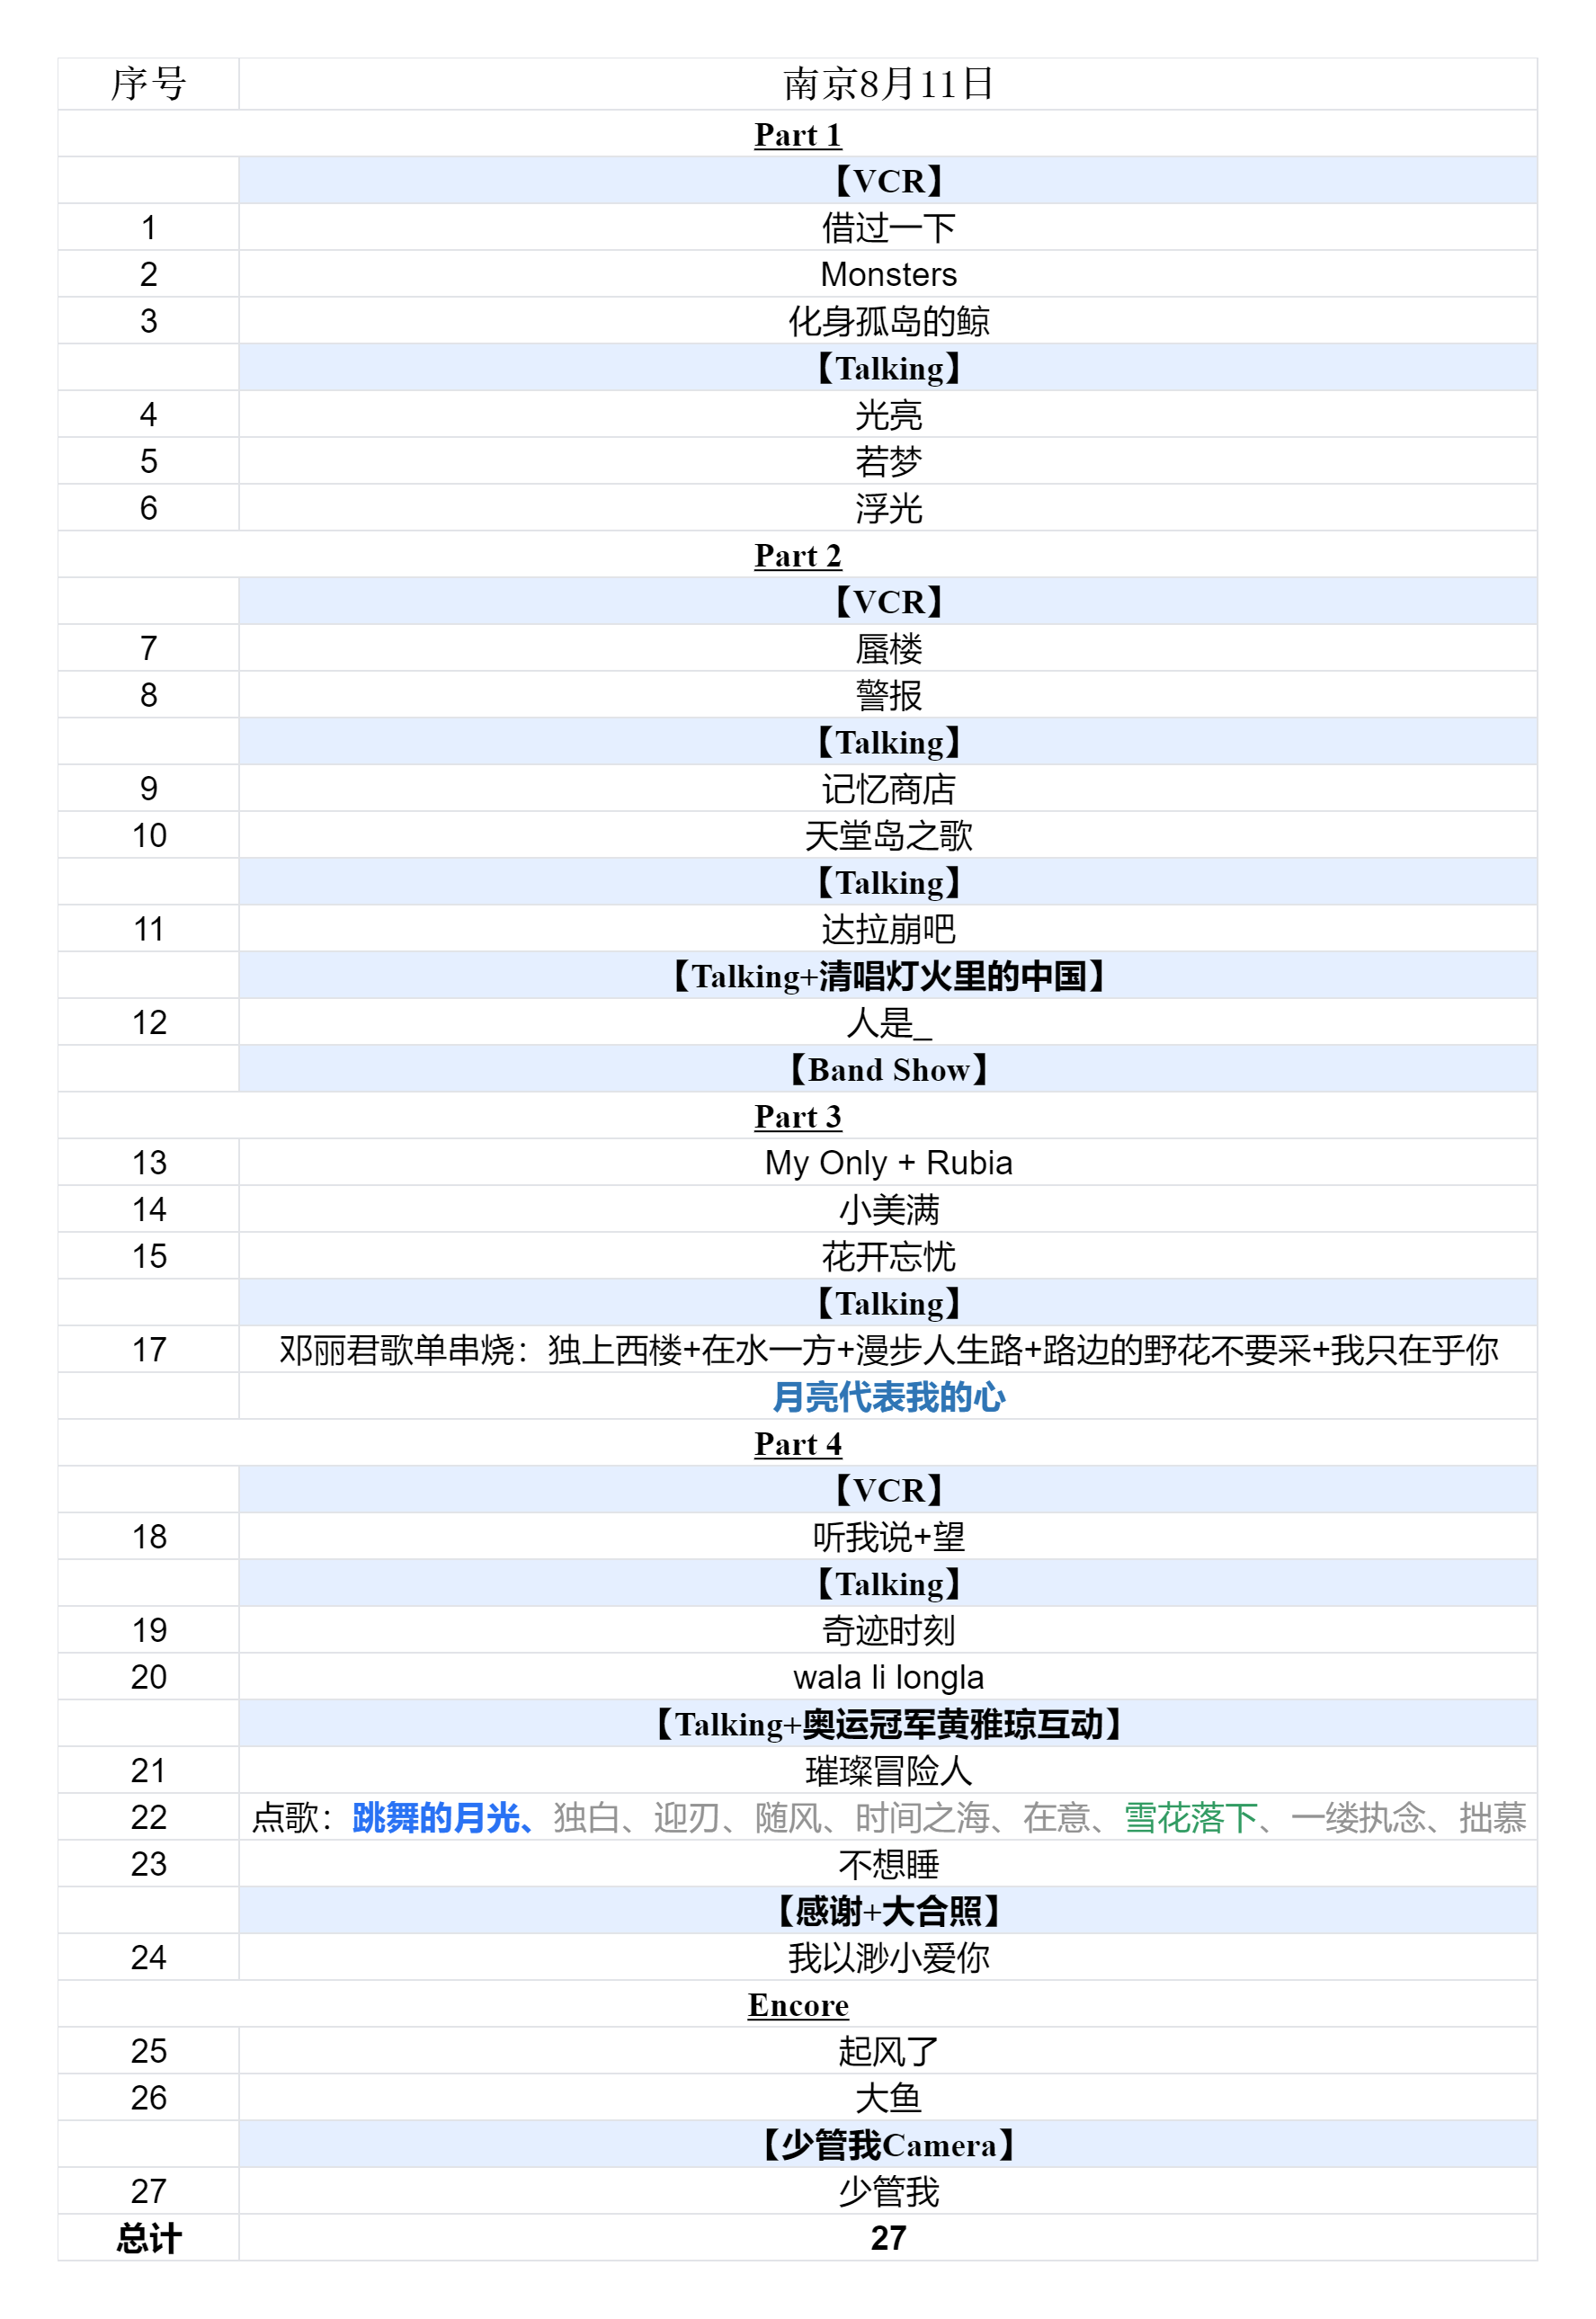
\includegraphics[width=330pt]{img/playlists/playlists-nanjing-20240811} 

}

\caption{2024周深9.29Hz巡回演唱会2024.08.11南京第二场歌单}\label{fig:unnamed-chunk-74}
\end{figure}

\newpage

\section{Part1}\label{nanjing-20240811-part1}

\hyperref[opening-vcr]{🎥【\textbf{开场VCR}】}

\hyperref[I-will-go-my-way]{🎵【\textbf{借过一下}】}南京的朋友们,你们好吗?

\hyperref[Monsters]{🎵【\textbf{Monsters}】}谢谢\textasciitilde{}

\hyperref[hua-shen-gu-dao-de-jing]{🎵【\textbf{化身孤岛的鲸}】}谢谢,大家好吗?化身孤岛的蓝鲸来到了南京,你们愿意跟我一起唱吗?(米:愿意\textasciitilde)到你们\textasciitilde 看台的\textasciitilde(深:我想给你能奔跑的岸头)(米:没有墙头)有墙头吗?(米:没有)起码一个墙头有吧?(米:没有)难道是说墙头多到数不清?(米:没有)(深:让你如同王后,谢谢你们一直在等候)

  南京的朋友们,你们好,看台的朋友,你们看得到我吗?让我听到你们好不好,大家好,我是歌手周深,欢迎来到9.29Hz演唱会,谢谢你们。宝你个头,怎么一开始就听到,谢谢大家,今天对我来说意义非常重大,因为这是我人生中第一次连开体育场,所以谢谢你们来跟我一起创造这个时刻,谢谢。我发现很多时候很多东西,我觉得,诶,我自己不相信的东西,我不相信自己有一天能够成为歌手,我不相信自己有一天会被看见,甚至不相信自己有一天可能,可以开演唱会,甚至是体育场。但是因为遇到你们,所有的不相信都让我相信,谢谢,那是因为你们的光亮都照在了我的身上,让我无论如何的转身,我都发现好像都很安全,谢谢你们。在此之前,这首歌我觉得要有一个小考题,让我看一下,(深:莫听穿林打叶声)下一句(米:一蓑烟雨任平生)但是如果这是一次语文考试的话,下一句应该写,(米:何妨吟啸且徐行)哈哈哈,你们太棒了。没错,何妨吟啸且徐行,希望大家,喜欢听歌我非常荣幸,但是就是要接诗句的时候,或者接考试的时候,大家一定不要记错,下一句是何妨吟啸且徐行好吗?看台的朋友,你们好吗?(米:好)无论你们在哪里,你们都是我的光亮,谢谢你们。

\hyperref[silver-linings]{🎵【\textbf{光亮}】}\textbf{我爱你们!}希望我们无论任何时候都能够像伟大的文学家苏轼一样,人生当中遇到任何狂风骤雨,我们都可以平稳自己的脚步,用最好的心态去面对一切,好吗?(深:光亮你自己)

\hyperref[ruomeng]{🎵【\textbf{若梦}】}愿意跟我一起唱吗?(米:愿意)谢谢\textasciitilde 到你们\textasciitilde 看台的朋友\textasciitilde(深:如我虔诚合十双手)你们(米:唯愿你能得到拯救)你们唱得太棒啦,这边的朋友准备好了吗\textasciitilde 到你们啦\textasciitilde 后面的朋友\textasciitilde 到你们\textasciitilde 全场跟我一起\textasciitilde 大声点\textasciitilde 看台的朋友(米:唯愿你能得到拯救)(深:因为你们,我才得到拯救)你们唱的若梦太好听啦。

\hyperref[floating-light]{🎵【\textbf{浮光}】}宝你个头\textasciitilde 跟我一起(深米:浮光掠影重山彩云间)\textbf{人生恍惚三万天,因为遇见了你,每一秒都不想错过\textasciitilde{}}

\section{Part2}\label{nanjing-20240811-part2}

\hyperref[senself-vcr]{🎥【\textbf{反深代词VCR}】}

\hyperref[mirage]{🎵【\textbf{蜃楼}】}

\hyperref[the-giver]{🎵【\textbf{警报}】}谢谢老师们\textasciitilde{}

  南京的朋友们晚上好,我是周深,南京的朋友有多少?南京朋友?那外地的朋友呢?哈哈哈,辛苦大家,你们辛苦啦。刚才非常荣幸的是唱了自己新专辑(米:反深代词),谢谢你们知道这张专辑,自己专辑反深代词里面的两首歌是一个比较新的,大家不是很熟悉的周深的一面,也谢谢你们能够让我有安全感,愿意让自己去介绍一个更立体或者是更多自己私人情绪的一个周深。因为很多时候自己要把自己情绪去告诉别人的时候,其实最害怕的是别人会觉得,啊?不至于吧?啊?你这是什么意思?啊?矫情。哈哈哈,但是我非常感动的是,当我把我所有的一些情绪放到反深专辑里面,12首歌里面,变成12个碎片的时候,发现我的歌迷、我的生米,他们会说,啊,原来周深有这一面,啊,原来周深这一个碎片,跟我好像,所以谢谢你们愿意跟我同频,也谢谢你们给我安全感,让我去感受一个更加立体的自己,谢谢你们,当然也希望的是你们可以找到跟你们熟悉的那一块碎片,然后去好好地更好地照顾好自己,好吗?(米:好)

  接下来有一个难题,就是还是想唱一首专辑里的歌,稍微耽误一下大家的时间。但是我想唱,我想唱《嗨》,我也想唱《记忆商店》,所以你们帮我做一个选择,等一下,我听一下哪个的呼声更大。这么多人喊嗨,我们记忆商店是不要面子的嘛。至于两首歌都没有听过,你也觉得看这两个名字哪个更合你的眼缘,你就选择。好,看台的朋友你们听到了吗?(米:听到了)听到了,好,要由你们选择这首歌哟,想听嗨的告诉我(米:啊啊啊)。记忆商店,我就对不起你了。想听记忆商店的告诉我(米:啊啊啊啊啊啊)。记忆商店比较大声耶,好像。谢谢你们,每一次跟你们相遇都是我最幸福的时刻,希望200年后我也可以去记忆商店去把我们最美好的回忆保存好,谢谢。我以为,刚才我都以为嗨就决定是要唱他了,人生还是有很多的惊喜,那我们一起来做好这一份美好的回忆吧。(米:好)

\hyperref[the-memory-store]{🎵【\textbf{记忆商店}】}

\hyperref[haven-song]{🎵【\textbf{天堂岛之歌}】}谢谢老师,叮咚你逃不出去,但是我进入到你们的记忆当中之后,我发现我逃不出去,那你们有没有逃出去?(米:没有)谢谢,谢谢,谢谢\textasciitilde{}

  那接下来这首歌我很喜欢,也是很多人就是第一次听到我的声音的一个舞台,尤其是小朋友。而且好像我之前还有在流媒体上面有看到说有个小朋友特别希望我能够穿那个SSR的皮肤,那个灰色的那个皮肤。这首歌叫做达拉崩吧,大家有听过这首歌吗?(米:有)那等一下你们要帮助我去讲好这个土话故事哦,好吗?(米:好)这个故事的主人翁叫做(米:达拉崩吧斑得贝迪卜多比鲁翁)记性很好。那这里面的恶龙的名字叫做(米:昆图库塔卡提考特苏瓦西拉松)你们完全都不用提词器,你们给不给我面子啊?那,就考一个难的,他们回到的那个城市叫做?那到底是发生一部什么样的故事呢?看台的朋友有听过吗?我们一起来看一下是发生了什么事情吧?

\hyperref[dalabengba]{🎵【\textbf{达拉崩吧}】}现在需要你们来给我讲好这个故事了,好吗?(米:好)快想一下,是谁打败了谁?救出了谁?他们又回到了哪里?到底发生了什么事情呢?于是(米:达拉崩吧斑得贝迪卜多比鲁翁)砍向(米:昆图库塔卡提考特苏瓦西拉松)然后\textasciitilde 咬了\textasciitilde 看台的朋友\textasciitilde{}

  谢谢大家,你们唱的太好啦,给自己一点掌声。我很开心的是很多人会在我的一些舞台上去认识我,然后也有很多机会可以在电影里面陪伴大家。我觉得唱OST是一个很幸福的事情,可以参与很多像导演、所有工作人员们,给观众朋友们制造的一个梦幻中。当我唱那首歌,我就发现好像自己也是在跟大家一起创造一个美丽的梦。但是也谢谢你们,因为你们为我创造了无数甜蜜的梦,谢谢你们。那我就想问了,接下来这首人是你们会唱吗?我上次已经被吓到,居然会,你们真的会唱吗?(米:会)试一下好吗?(米:好)那我们试一下这首歌。(灯火里的中国青春婀娜,灯火里的中国胸怀辽阔,灯火灿烂的中国梦,灯火荡漾着心中的歌),哇,给自己掌声,你们唱得好听,你们都特别棒,但是无论怎么样,我觉得我们都可以创造很多非常非常美好的事情,我们都是最棒的那个人。流浪地球的歌人是\_,希望你们喜欢。(米:宝贝)宝你个头\textasciitilde{}

\hyperref[renshi]{🎵【\textbf{人是\_}】}这边的朋友,你们好吗?(米:好\textasciitilde)(深:可仍夺不走我的选择)到你们(米:弹指间湮灭我\textasciitilde)谢谢你们\textasciitilde{}

\section{Part3}\label{nanjing-20240811-part3}

  你们好吗?(米:好)你们猜一下我在哪里啊?有人说对了答案耶,我在你们的心里啊,你们再认真的看一下我在哪里,找到我了吗?我在这个非常漂亮的光束组成的树里,这些光都是来源于你们啊。没想到这么快就到了我的弹唱的时间了。我想告诉大家任何时候想学一门新的一个技术,或者是想学一个自己感兴趣的事情都不会晚,因为我现在也老大不小,哈哈哈,也在尝试学这样一件事情,所以等一下希望你们能够用你们的爱来鼓励我,好吗?(米:好)不会还有人在找我在哪里吧,我在这里,看到我的给我一个呼唤,(米:啊啊啊啊)谢谢谢谢。等一下我唱的这些歌我觉得是非常温馨,非常温暖的歌曲,希望你们能够喜欢,好吗?(米:好)

\hyperref[my-only]{🎵【\textbf{My Only}】}

\hyperref[rubia]{🎵【\textbf{Rubia}】}谢谢你们看到了我\textasciitilde 你们好吗?(米:好)看台的朋友呢?(米:好)(深:A Madder there for you you you you\textasciitilde)谢谢大家\textasciitilde{}

  刚才两首歌有很多人都告诉我非常的治愈和救赎,但我发现任何治愈的片段和任何救赎的音乐,都不如我看到了你们。虽然昨天是七夕节,但是我觉得那份爱,那份温暖不应该仅仅是停留在昨天,对不对?就像我昨天晚上就抱着一种非常不舍的状态说的最后一句话,希望我们的快乐和甜蜜,我们的爱不只是在七夕,而是在每一个朝夕。让我们来听一下接下来这首歌是什么吧?

\hyperref[happy-ending]{🎵【\textbf{小美满}】}会唱吗?(米:好)来跟我一起唱好不好?(米:好\textasciitilde)后面的\textasciitilde 跟我一起哦\textasciitilde 遇到了你们是我最美的答案\textasciitilde 看台的朋友\textasciitilde 太棒啦\textasciitilde 看台的朋友大声唱哦\textasciitilde 大声点\textasciitilde 看台的朋友\textasciitilde 你知道吗?你们每个人的力量其实都非常非常的大,你们每个人的光芒都非常的耀眼,你们让一个非常普通的男孩子去靠近他的梦想,从周边的舞台再到一个个越来越大的舞台,最后在体育场跟大家相见,所以你们要相信自己好吗?(米:好)小美满,我觉得我被你们听到,被你们选择是我今生最大的美满。这首歌每次一听的时候都觉得所有的愿望都会实现,所以我们一起来许愿吧,好吗?(米:好)像我这样闭上眼睛许愿,321,我们的愿望就会被听见。现在无论你是什么职业,什么年龄段,跟我闭上眼睛,听话,闭上眼睛,默默想想现在的心里,想许的那个愿望,想想你要许什么愿望呢?闭上眼睛哦。但是这个愿望有一个要求,只能够关于你自己,想一想很多时候是不是在繁忙的节奏当中忘记问候一下自己呢?想好了吗?321,睁眼\textasciitilde(深:你愿相信什么,就把世界 看成什么样\textasciitilde)全场(米:自己就是自己最好的陪伴)(深:\textbf{生米就是周深最好的陪伴})\textbf{我爱你们!}

\hyperref[no-worries]{🎵【\textbf{花开忘忧}】}(深:若记忆被偷走了忘了我的爱,我会说)(米:你好啊)南京,你好\textasciitilde(深:别走远了 一起回家)我会努力到你的家里来看你的\textasciitilde 以前我会害怕我的想念,我的思念,离开的人会听不见,但是现在我好幸运有你们愿意跟我一起表达这份思念,他们一定听得见的,对吗?(米:对)花开忘忧,愿你无忧,花开忘忧,(米:愿你无忧)谢谢\textasciitilde{}

  (深深换衣服,米:啊啊啊啊)等一下,我的情绪起伏,哈哈哈,太考验一个人,我还在呜呜呜,我觉得我们每个人都是在宇宙大爆炸的时候散落在人间的星辰,你们都是最美丽最闪亮最漂亮的那一颗星,你们要记得哟。然后要说到启蒙我唱歌,或者是让我觉得,哇原来还有一个语言是可以用唱歌来表达的这么美好,一定就是应该算是我的一个目标,一直觉得在闪耀着我唱歌的那颗星星,她就是邓丽君女士,你们听过她的歌吗?(米:听过)我也特别特别希望自己能够成为一位像她这样,有趣,然后又唱歌非常好,然后每首歌里好像都藏着每一个人的时光,每首歌都像一颗时光胶囊。我会继续努力唱歌的,歌手周深一定会继续努力唱歌的好吗?(米:好)谢谢你们,那如果等下你会唱的话跟我一起唱哦(米:好)看台的朋友们,你们听到了(米:听到了)谢谢\textasciitilde{}

🎵【\textbf{邓丽君组曲}】
\hyperref[one-in-the-building]{🎵【\textbf{独上西楼}】}跟我一起唱哦\textasciitilde{}
\hyperref[on-the-water-side]{🎵【\textbf{在水一方}】}
\hyperref[walk-the-road-of-life]{🎵【\textbf{漫步人生路}】}你们太棒了,摇起你们手中的荧光棒,这边的朋友看到了吗?这边的朋友\textasciitilde 嗨起来\textasciitilde{}
\hyperref[only-with-me]{🎵【\textbf{路边的野花不要采}】}到你们喽\textasciitilde(深:虽然已经是百花开)知道你们墙头多,所以我也很执着(米:路边的野花)要干嘛呀?(米:你不要采)(深:噔噔噔噔噔噔噔噔\textasciitilde)你们会忘记我吗?(米:不会)
\hyperref[only-you]{🎵【\textbf{我只在乎你}】}(米:除了你我不能感到一丝丝情义)我才是(深:除了你我不能感到一丝丝情义)

\hyperref[my-heart-is-moon]{🎵【\textbf{月亮代表我的心}】} 谢谢你们,\textbf{希望任何时候你们都可以感觉到我的爱,就像月亮一样,有的时候可能你看不见,但是我都一直在好吗?}(米:好\textasciitilde)无论你在哪,我都在这,不要害怕孤单好吗?(米:好)

\section{Part4}\label{nanjing-20240811-part4}

\hyperref[thank-you-vcr]{🎥【\textbf{谢谢南京,谢谢你VCR}】}

\begin{figure}

{\centering 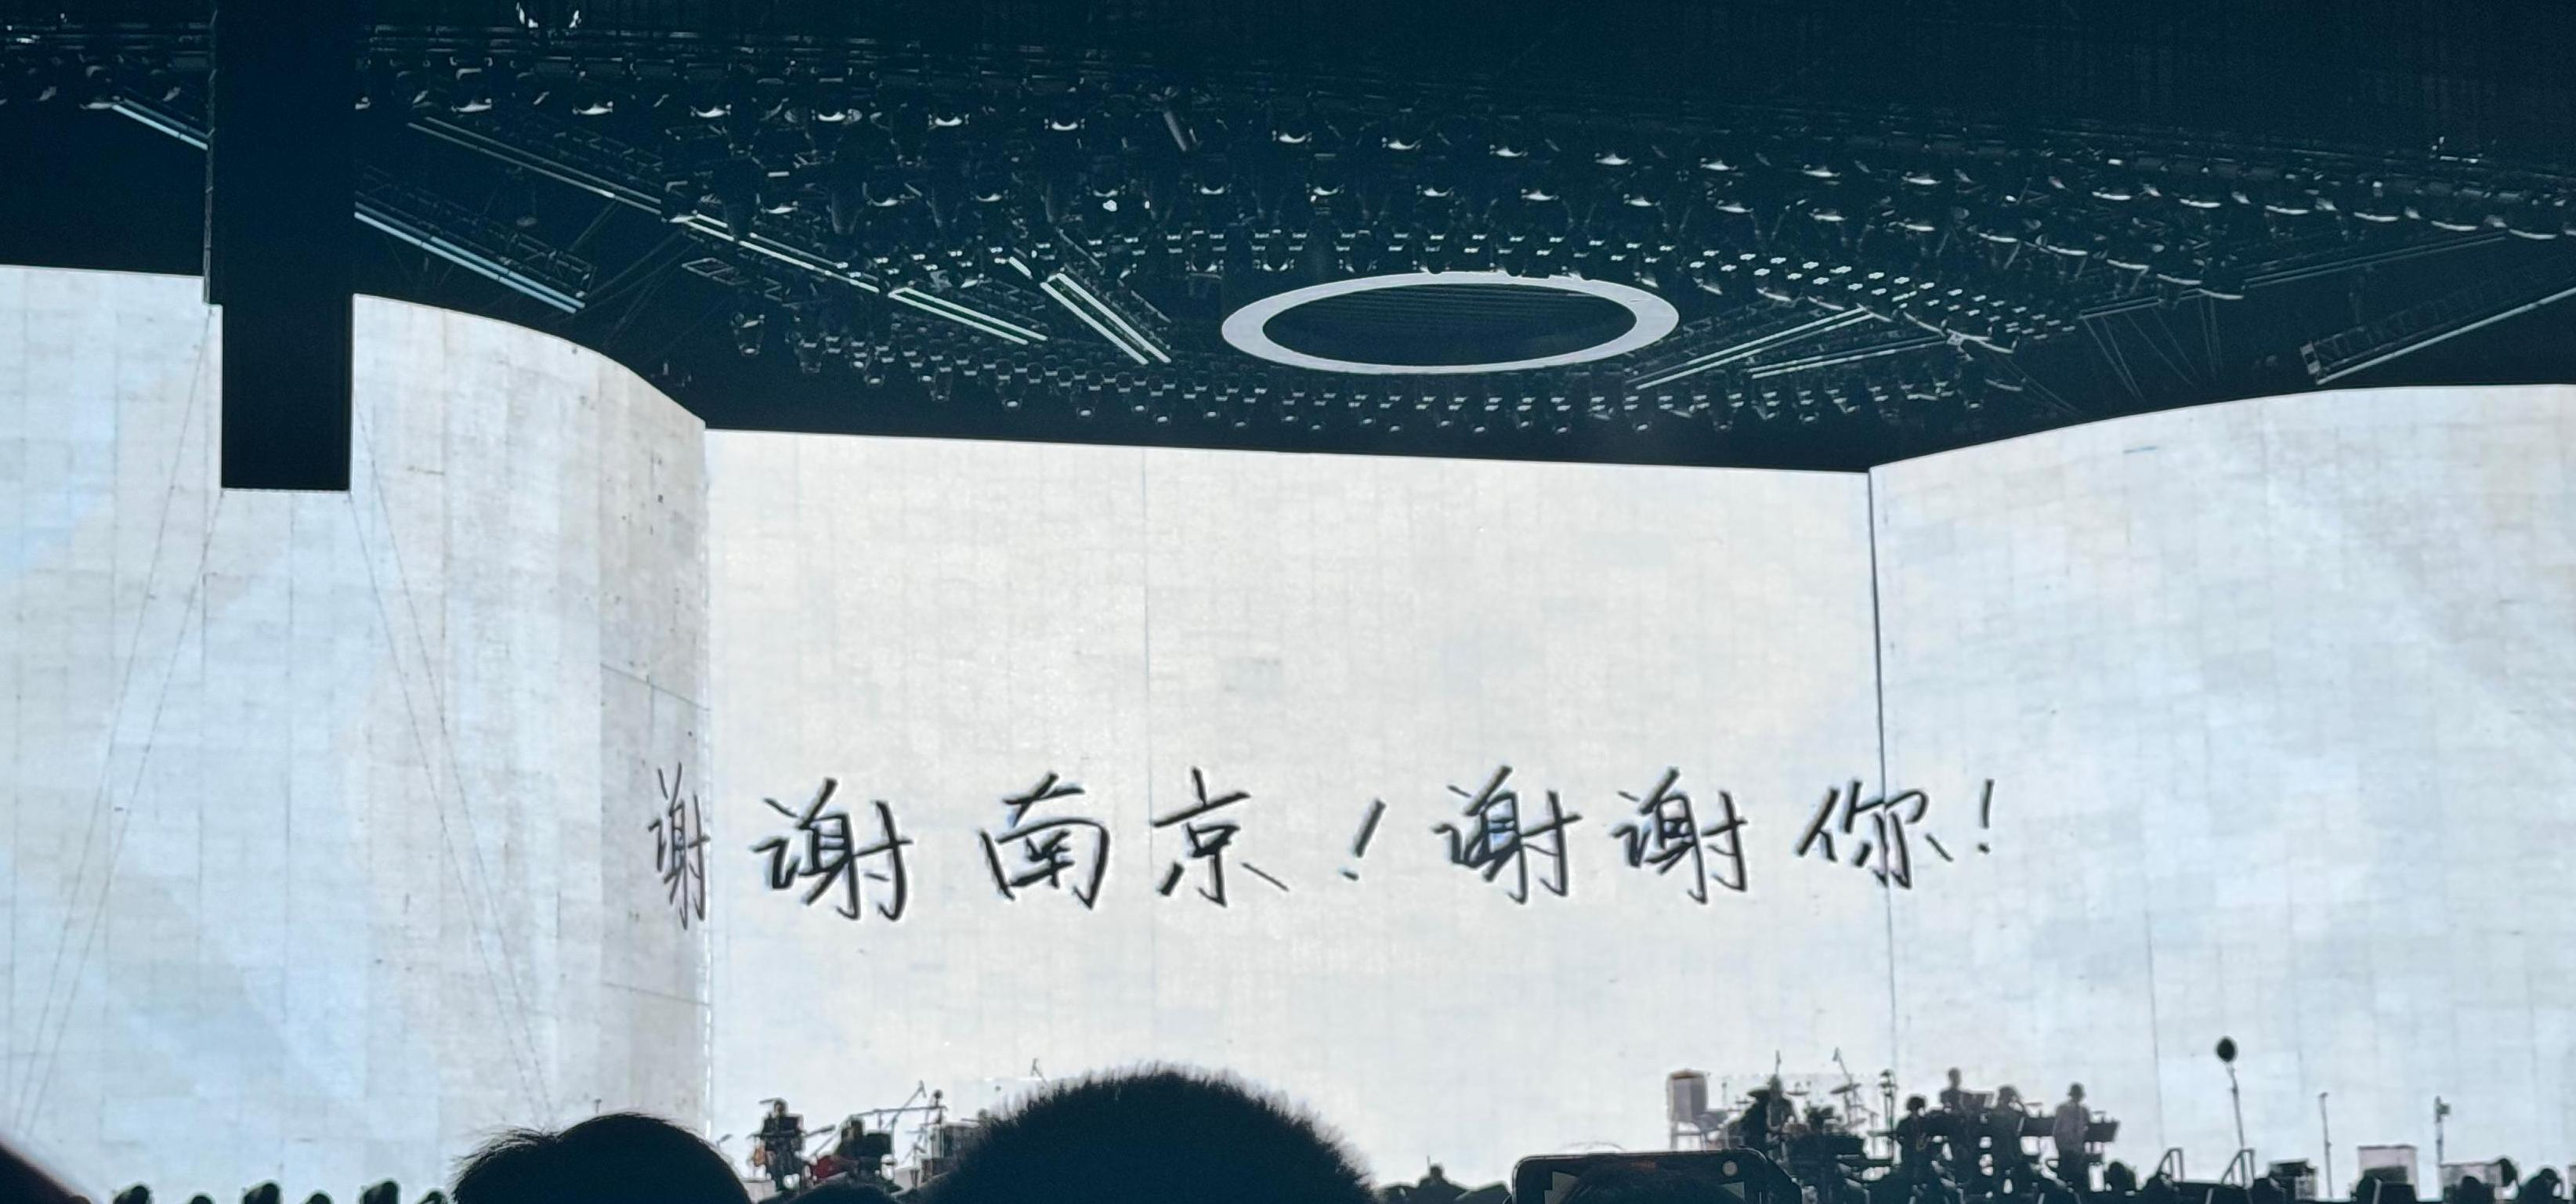
\includegraphics[width=400pt]{img/nanjing20240811/thank-nanjing} 

}

\caption{谢谢南京!谢谢你!}\label{fig:unnamed-chunk-75}
\end{figure}

\hyperref[listen-to-me]{🎵【\textbf{听我说}】}谢谢你们听我说,我也想听你们说,好吗?(米:好\textasciitilde)做你们有意义的空壳,我也非常非常有意义!(深:那个人总会懂的,那个人也能是我)

\hyperref[hope]{🎵【\textbf{望}】}看台的朋友,你们好吗?一起\textasciitilde 看台的\textasciitilde 最大的声音(米:我们总会 绕啊绕 绕啊绕\textasciitilde)你们(米:手中线 绕啊绕 绕啊绕)无论你们在哪儿,在做什么,你们都要知道,我都在这里陪着你们,好吗?(米:好)因为遇到了你你你你你你你你你你你你你你,(深:我才心有所住,你们永远不会孤独)

  好开心又和你们见面啦,我觉得以前我们很像,就是最熟悉的陌生人,我们就像是网友,可能看到过彼此的ID,但是不知道就真的会有这样浓的一股温暖会存在,他会来,就跑到那么远的地方来见你,无论是动车延误,或者是飞机延误,或者那么热的天气,或者任何的天气,我觉得我们能够相见都是最大的幸福。我不敢相信这些会实现,但是我没有想到你们出现在这里啦。我,说实话,我其实有一点点,就是大家听过一个词叫做不配得感吗?对,就很多时候,所以就是我在想的是我一定要好好的照顾大家,我想要做更多之类的,但后面发现你们给我的永远都要多的多的多的多。(米:你配)你们让一个以前就是真的不敢在那么多人面前唱歌的男孩,到现在能够在体育场开他自己人生当中的第一次,连续两天都开体育场,而且两天都来满了人,谢谢你们。谢谢你们,如果一定要形容这个时刻,我觉得只能用四个字去形容它,因为它是绝对的奇迹时刻。看台的朋友,你们也是奇迹时刻的一部分,知道吗?我指到哪里如果都有尖叫的话,那应该很奇迹哦\textasciitilde{}

\hyperref[magic-moment]{🎵【\textbf{奇迹时刻}】}看台的朋友\textasciitilde【魔术时刻】南京的朋友们,你们好吗(米:好)我为大家准备了一束花,但是需要你们的爱它才能开花,可以让我听到吗?(米:啊啊啊啊)这些花不仅仅是要七夕的时候才收到,每一份爱在每一天都要感受到哦,大家还记得,每个人的手上都会有一颗种子吗?那相信大家可以种出很多美好的奇迹,我们要浇点水,然后用爱的呼唤它,321,快乐不该只是在七夕,而是每一个朝夕,对不对?(米:对)

\begin{figure}

{\centering 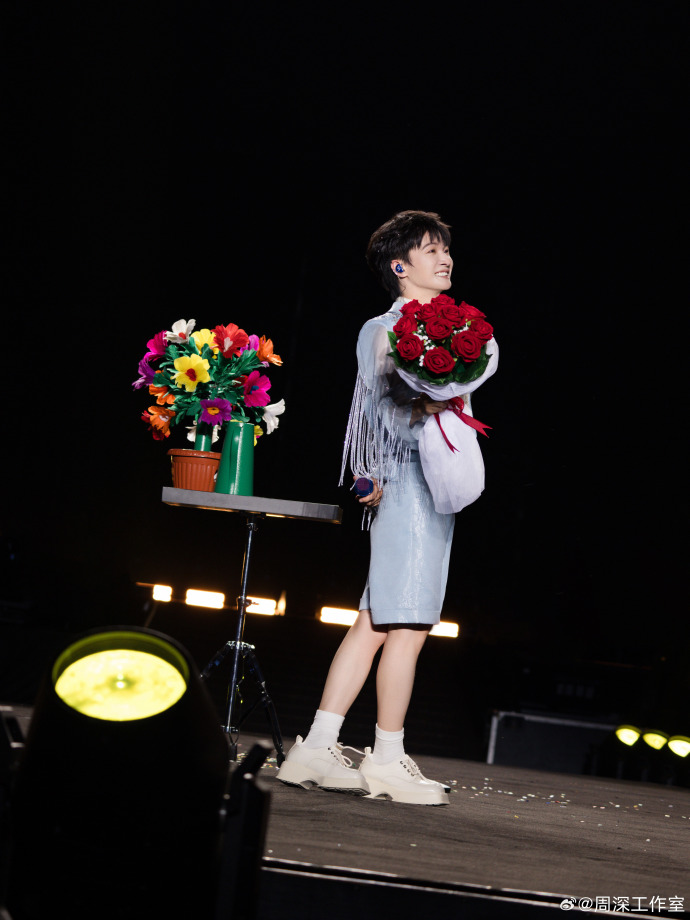
\includegraphics[width=450pt]{img/nanjing20240811/001} 

}

\caption{快乐在每个朝夕 【@weibo-charlie-studio】}\label{fig:unnamed-chunk-76}
\end{figure}

  你们开心吗?(米:开心)糟糕糟糕,我都害怕一年就是巡演完之后,我真的会Magic,但是我觉得能够听到你们的欢乐,你就是我最荣幸的Magic,谢谢。在新专辑当中还有一首歌,大家会问它,诶?这个名字叫什么?什么意思?它其实是一个快乐的密码,就当你喊出这个密码的时候,你就可以把所有的沟通障碍全部都清除,整个世界都会变得非常非常简单去沟通。比如看台的朋友,你们好吗?那如果用快乐密码的话,就是wala li longla。明显感觉到快乐人就更多了,那等一下跟我一起来享受这一份快乐,好吗?(米:好)我们全场来一遍,wala li longla,(米:wala li longla)你们太棒啦\textasciitilde{}

\hyperref[wala-li-longla]{🎵【\textbf{wala li longla}】}看台的朋友,嗨起来\textasciitilde 全场学会这个密码了吗?等下我们一起来念,好不好?(米:好)\textbf{感受这一份快乐吧,我最爱的你们},来喽。wala(米:wala),wala li(米:wala li),wala li long(米:wala li long),wala li longla(米:wala li longla),wala(米:wala),wala li(米:wala li),wala li long(米:wala li long),wala li longla(米:wala li longla),wala(米:wala),wala li(米:wala li),wala li long(米:wala li long),wala li longla(米:wala li longla)\textbf{你们是全世界最棒的},我们再来连唱一句,Ah,唱,(米:Ah)再来,Ah\textasciitilde 全场,321,(米:wala li longla)谢谢你们,掌声给到舞蹈老师们,要表达快乐的话用321(米:wala li longla)

  哇塞,你们太棒了,给自己一点掌声。哇,我没想到,这是南京的第二场,我还担心自己能不能hold住这个台子,后面发现你们帮我hold住了,太喜欢你们了,而且我记得当时在武汉场的时候,好像是奥运开始的前几天我们一起就是给他们加油打气,对不对?还有人记得吗?今天如果没有记错,好像,诶,真的还挺有缘的,他好像是奥运比赛阶段的。应该算是最后一天或者最后一两天这个日子,而且今天我们现场有来奥运冠军哦,她是羽毛球混双的女生冠军哦。可以给她个麦克吗,我们掌声欢迎我们的雅琼妹妹,她厉不厉害?我们是不是也感觉到非常的骄傲?(米:是)我们是不是要谢谢她?也要谢谢我们所有在绽放自己的运动员们,对不对?(米:对)

  麦克到了,给大家打个招呼吧。(雅琼:哈喽,大家好,我是黄雅琼)哇塞,而且之前,我们在后面打招呼时候,雅琼跟我说,你之前也有自己抢票去看成都场是吧,(雅琼:太难抢了,我觉得大家应该都知道吧,就是深深的票好难抢,加场\textasciitilde)(米:加场加场加场\textasciitilde)我会加油的,诶,我很好奇你是,您今年听我的歌听了多少年?哈哈哈(雅琼:其实我是在那个,诶,有点紧张)大家掌声鼓励她。(雅琼:我其实是在卡布时期就已经在听了)卡布时期,我解释一下,就是在我出道之前我就喜欢自己录歌发到网上,那个时候名字叫做卡布。哇,那你听了有十多年了诶,(雅琼:但是因为训练的原因断断续续,不好意思),不会,但是你觉得能够陪伴你训练或者是任何时候,或者任何时候陪伴你们都是我最大的荣幸。谢谢雅琼妹妹,谢谢你们。(雅琼:谢谢深深)而且就是好像不止收获了金牌,收获了一钻。方便跟大家打个招呼吗?这两天还真是充满甜蜜的一天。(雅琼:昨天可惜没有来了)不会,我觉得每天都应该要甜蜜,不仅仅是一个节日才甜蜜,好不好?谢谢您。谢谢。(雅琼:我还想再说一个故事,就是奥运会前我不是去了成都嘛所以就关于这个小美满这个愿望,我当时是许了一个愿望的,就是因为属于自己嘛,就想说)对,必须许关于自己的愿望(雅琼:对,就想说拿这个奥运冠军,所以说愿望真的会实现哦)谢谢,但我觉得一切都是你的努力以及你所有的付出,很开心看到你的努力得到回报,(雅琼:谢谢)对,谢谢你,我们全场再一次谢谢她,好不好?谢谢谢谢,谢谢雅琼,(雅琼:谢谢)谢谢谢谢。然后我觉得我们每个人也都像运动员一样,但我们的人生道路中不停地去拼搏、去努力,我们有很多时候属于我们自己的备战时刻,或者是属于我们很多时候自己的那个就是,被折叠到了,自己在努力付出的时刻,但是不要害怕,我们每一个璀璨冒险人一定是可以收获属于我们的璀璨,对不对?(米:对)看台的朋友你们听到了吗?璀璨冒险人们,向前冲吧\textasciitilde{}

\hyperref[adventurers]{🎵【\textbf{璀璨冒险人}】}跟我一起\textasciitilde{}\textbf{\textcolor{red}{我爱你们} }(深:沿途一身泥泞 跌撞的是我\textasciitilde)璀璨冒险人们,周深可以,你一定也可以\textasciitilde(深:不惧脆弱)我们(深、米:不惧脆弱)谢谢\textasciitilde{}

  谢谢,谢谢你们,谢谢,再一次掌声给我们的舞蹈老师们好不好?还要用更热烈的掌声给最棒的你们自己。

【\textbf{点歌环节}】接下来到点歌环节,还是那句话,不要高兴得太早,很有可能你没有听过那些歌,哈哈哈,但是这个歌单,但是这个歌单它都是我心中很喜欢的歌,而且我也相信它一定是,可能就是某一个人,某一个你心中的宝藏歌单,对不对?来喽,这里有9首大家可以看一下,独白、迎刃、跳舞的月光、随风、时间之海、雪花落下、在意、一缕执念、拙慕,有你们喜欢的吗?全场要倒数5个数字,我们的摄像老师就会捕捉到他,好不好?(米:好)摄像老师捕捉起来,你们仿佛就是宠物小精灵,就要用那个精灵球。全场,5(米:4321)停,哎呀,你在哪?(在这里)你这个声音我仿佛感受到了上天的呼唤,这里,嗨喽,你好你好,我们怎么称呼?(你叫我小马)小满?(小马)小马,小马你好,方便问就是听我的歌多久了吗?(19年)19年听的歌,那到现在差不多5年左右。(19年10月份)那你听我的第一首歌是?(Monsters)是那个我们的歌?(综艺)我们的歌里面的Monsters是不是?(是的)我没想到过这首歌让这么多人认识到我呀。那有没有其他人也听过这首歌?谢谢你,你是哪里的朋友?(江苏的,是在南京)江苏的?就是南京的?我要验证一个事情,就是我来到南京,学了一句南京话,(我不是南京本地的)你自己聊吧,哈哈,不会,谢谢,那你是在这里读书还是?(对对对,在这里5年了)在这里5年了,喜欢这里吗?(喜欢)很棒很棒。所以你是也是江苏的,所以这里的口味又比较符合一点点。好,谢谢你,那这上面有你喜欢的歌吗?(有)哪一首?(每一首)我想说就是我觉得很亲切的,就是我看到你有很多蓝色的元素。对,然后我们的雅琼妹妹那边她好像也有那个蓝色。就有一次我在坐飞机的时候,大家有看到那个图吗?就是一个扎着那个蓝色的辫子,然后背了个包,上面挂着周深,在背那个上面就是这个时代不能没有周深,哈哈哈。然后他就在我前面一起登机,然后我就,哎呀,好尴尬呀,然后她也没有很在乎后面是谁来着。然后这一切就非常的安静,那个时候的空气已经凝固,就是凝固到我心里很焦灼,就是怎么办?好尴尬,我该怎么办?我跟她打招呼吗?还是应该怎么样呢?``我先登机了哦''哈哈哈哈哈哈,好的,那你要听哪一首?请点一首?(3号跳舞的月光)为什么会选择这一首?(从上海场我就想听这个)哇,你上海场就在啊?你好厉害啊(我昨天也在)谢谢你,但是务必记住,在好好的相遇之前一定要好好的,干嘛?照顾好自己好不好?(好的),谢谢小马,谢谢你,(可以再说一句话吗?)说什么?等一下,说吧(宝贝,你一直唱,我一直在)谢谢小马,宝你个头啊,宝你个头啊乘以3.4w。跳舞的月光\textasciitilde{}

\hyperref[dancing-moonshine]{🎵【\textbf{跳舞的月光}】}(深:你能听见我吗)(米:能\textasciitilde)你们能听到我吗(米:能\textasciitilde)记住我好吗?(米:好\textasciitilde)分开之后会想念吗?(米:会)\textbf{我也会非常非常想念与你见面的时光。}(深:你能听见我吗)(米:能)

\hyperref[keep-playing]{🎵【\textbf{不想睡}】}看台的朋友们\textasciitilde 谢谢这个宇宙让我们相遇啦,谢谢你\textasciitilde 跟我一起\textasciitilde 看台的朋友\textasciitilde 后面的朋友\textasciitilde{}

  这个宇宙非常非常大,但是我们在这里,先把手机的闪光灯关一下,因为可能会太热,哈哈哈,为了保护你们的手机,那我们在这里发出的每一个光子,都会在宇宙那传递很多很多年,也就是说不知道多少年之后,我们在宇宙的另外一端,我们又相遇啦,所以我们会一直都陪伴着彼此的,对吗?(米:对)那我们也有掌声给我们,让我们平平安安、快快乐乐见面的所有工作人员们,好不好?(米:好)感谢场地支持,南京奥体中心,感谢本次巡演的全程主办北京时代立方文化传播有限公司,哎呦,呼声很大哦,谢谢大家,谢谢你们,谢谢,南京承办方江苏中奥国际体育文化传媒有限公司。谢谢演唱会制作单位毕应,谢谢总导演周佑洋、庄惟惞,谢谢我们的音响总监金少刚,谢谢我们的音乐总监龙隆老师,谢谢我们的乐队老师们,谢谢我们的和声老师们,有一说一,做我的和声老师是有点辛苦的。哈哈哈,我们再一次谢谢他们。谢谢我们的舞蹈团队SDT ShowPro,谢谢服装团队设计师劳伦斯许工作室,谢谢时装品牌windowsen。谢谢我们的音响工程,南京奥斯泰视听科技有限公司,谢谢我们的调音团队乐尔工作室。谢谢硬体工程北京力超舞台集团,谢谢周深工作室的小伙伴们,糟糕,这呼声比我唱歌声音都要大,谢谢你,谢谢你,谢谢微博(米:倒闭),最终还是他承担了这一切,谢谢微博音乐(米:倒闭),谢谢微博演出(米:倒闭),我谢谢你们。感谢非常美的城市南京,谢谢南京所有职能部门的大力支持,保障我们这场演出的顺利进行,对不对?(米:对)感谢现场所有台前幕后的工作人员们,尤其也要感谢我们的志愿者们,好不好?(米:好)当然最最最最最最最最最最重要的就是感谢每一个到南京来我们一起见面的你你你你你你你你你你你,谢谢你们。

  话不多说,我们来合照吧,来,中间,321,耶,左边,321,先拍照,我的鞋子(鞋子掉了,哈哈哈),321,糟糕啊,我的增高垫,先不管,先跑过去,321,那边的朋友们好吗?(米:好)啊,好远啊,但是无论再远,我都会奔向你,321,我回头望,发现更远,现在领跑的是周深,(米:加油加油加油)是周深,\textbf{他是否能走向他的生米们呢?他做到啦!}人家还以为在这里办运动赛事,321,你们好,321,谢谢你们。

  宝你个头,刚才的不想睡,是卡布的晚安曲,周深也有一首他的晚安曲,叫做(米:我以渺小爱你)。谢谢你们看到了渺小的我,谢谢你们选择听到了我,谢谢你们。歌手周深真的很荣幸,真的很幸福,虽然他的力量很渺小,但是你却告诉我温暖了你,谢谢你,我以渺小爱你。

\hyperref[loving-you-in-my-humble-way]{🎵【\textbf{我以渺小爱你}】}爱你个头啊\textasciitilde 遇见你们这件事实在是太美了\textasciitilde 也许我在你人生当中出现的时间会很短,但是我很荣幸,非常荣幸能够出现那一秒、两秒或者是三秒,或者是一首歌的时间,(深:我以短暂爱你不朽的旅程)谢谢你们\textasciitilde{}

\section{Part5}\label{nanjing-20240811-part5}

\hyperref[the-wind-rises]{🎵【\textbf{起风了}】}谢谢你们还在,你们看啊,起风喽\textasciitilde 谢谢你们,谢谢南京\textasciitilde 谢谢你们\textasciitilde{}

\hyperref[big-fish]{🎵【\textbf{大鱼}】}谢谢\textasciitilde{}

  还想要不知道是否有这个荣幸,可以再唱一首自己专辑里的歌呢?(米:好)我们会有一个小小的互动环节,叫做少管我camera,也就是如果摄像老师捕捉到谁,就要做我们的标志性动作,叫做321,嘿,少管我,少管我,大家不要误解他,他不是争执,也不是任何的不开心的事情,他是明确的为自己负责,知道自己要成为一个什么样的自己好吗?(米:好)对,用开心的这个心情喊出,嘿,少管我,所有的不开心都会远离你。那我们全场倒数五个数字吧。5(米:4321)oh,你在哪里?(在哪里?)hello,你好,怎么称呼你,这里就可以用30分钟,高?高女士,你好,那你做好这个准备,要用你最大的声音,让全场都听到你的少管我了吗?没有?哈哈哈,来,321,嘹亮到我都以为这个声波过于高频,然后超过我们可以听到的声音,我们再试一次,我跟你一起,321,嘿,少管我,全程给他掌声。谢谢你,那我们全场能不能跟我一起来一遍啊?(米:好)这个所有的不开心都会远离你,全场321,(米:嘿,少管我)你们太棒了\textasciitilde{}

\hyperref[watch-ur-manners]{🎵【\textbf{少管我}】}大家都要好好的照顾好自己,好吗?(米:好\textasciitilde)全场,321,(米:嘿,少管我)54321,(米:嘿,少管我)你们太棒啦\textasciitilde 全场\textasciitilde 全场,321,(米:嘿,少管我\textasciitilde)看台的朋友,54321(米:嘿,少管我)谢谢你们,希望你们向最好的自己向前冲,好吗?(米:好)看台的朋友们,谢谢你,谢谢大家,谢谢你们,好好照顾好自己。54321(米:嘿,少管我)你们是最棒的,大家手机不要忘了,证件不要忘了,一定要健健康康,平安安到家,答应我好吗?(米:好)呦吼,希望这一份美好的回忆,在你任何需要的时候都会出现,谢谢,这边的朋友你们好吗?(米:好)54321,(米:嘿,少管我)你们是最棒的,大家注意安全,谢谢你们来跟我见面,谢谢你们看到了我,听到了我,也请你们相信自己一定会成为自己喜欢的那个自己的好吗?(米:好)谢谢你们,注意安全,证件不要掉了,手机不要掉了,一定要平平安安的,54321,(米:嘿,少管我),\textbf{我爱你们!}

\begin{center}\rule{0.5\linewidth}{0.5pt}\end{center}

\begin{figure}

{\centering 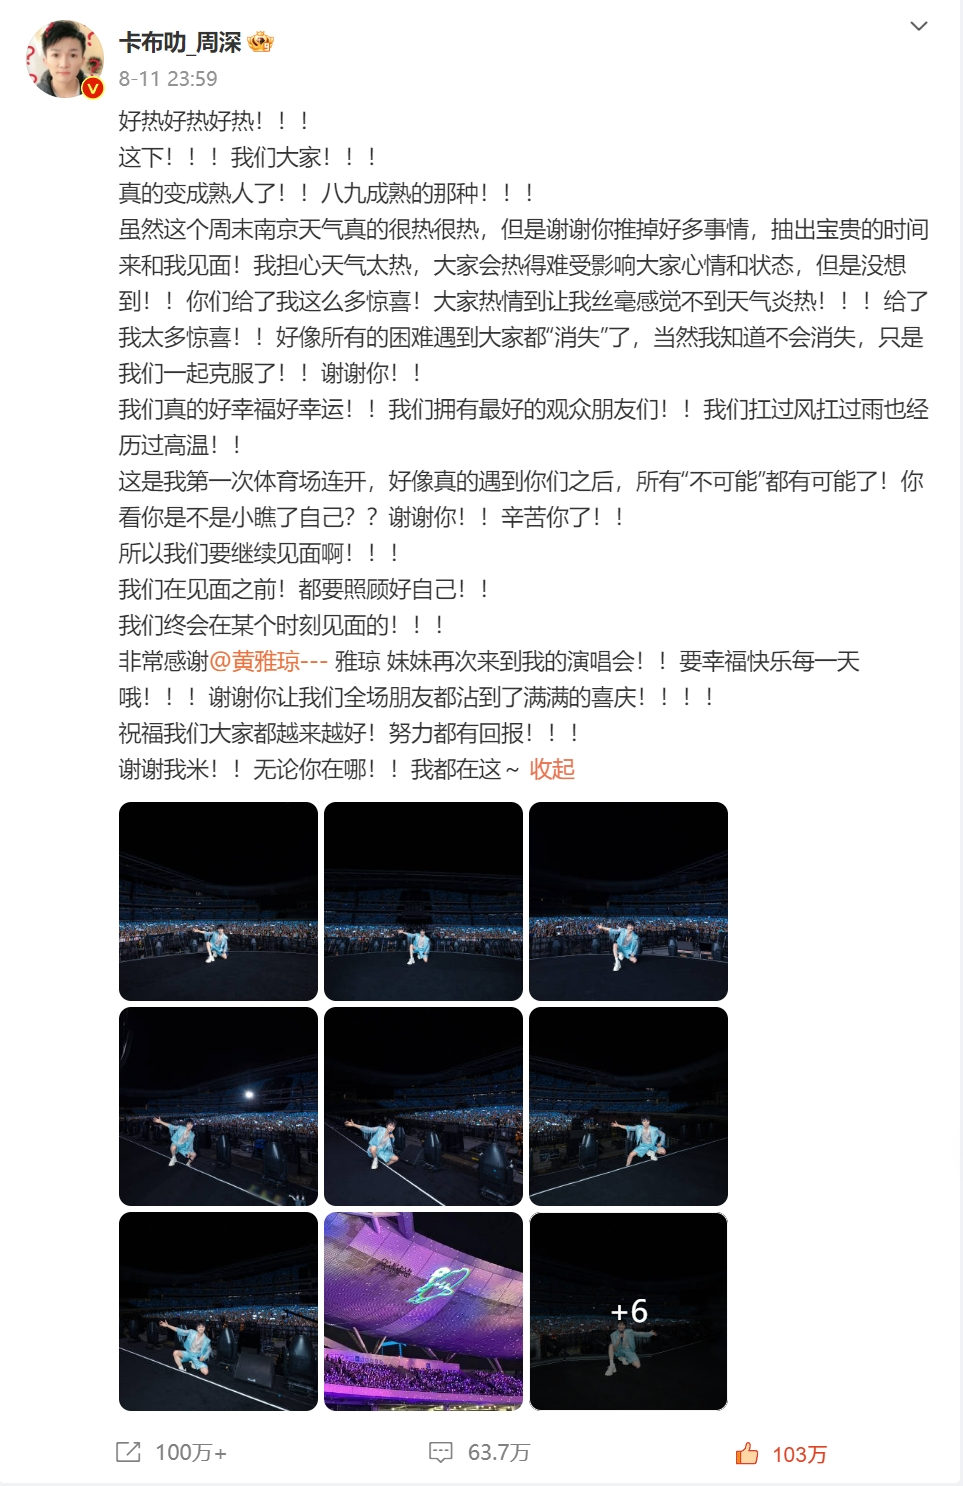
\includegraphics[width=400pt]{img/weibo/nanjing-20240811} 

}

\caption{周深南京奥林匹克体育场演唱会结束微博 【@weibo-charlie】}\label{fig:unnamed-chunk-77}
\end{figure}

\chapter{2024.08.23杭州场}\label{hangzhou-20240823}

\begin{quote}
\textbf{\emph{我很开心,我们的相见,我只等了10年。------ 周深}}
\end{quote}

\begin{figure}

{\centering 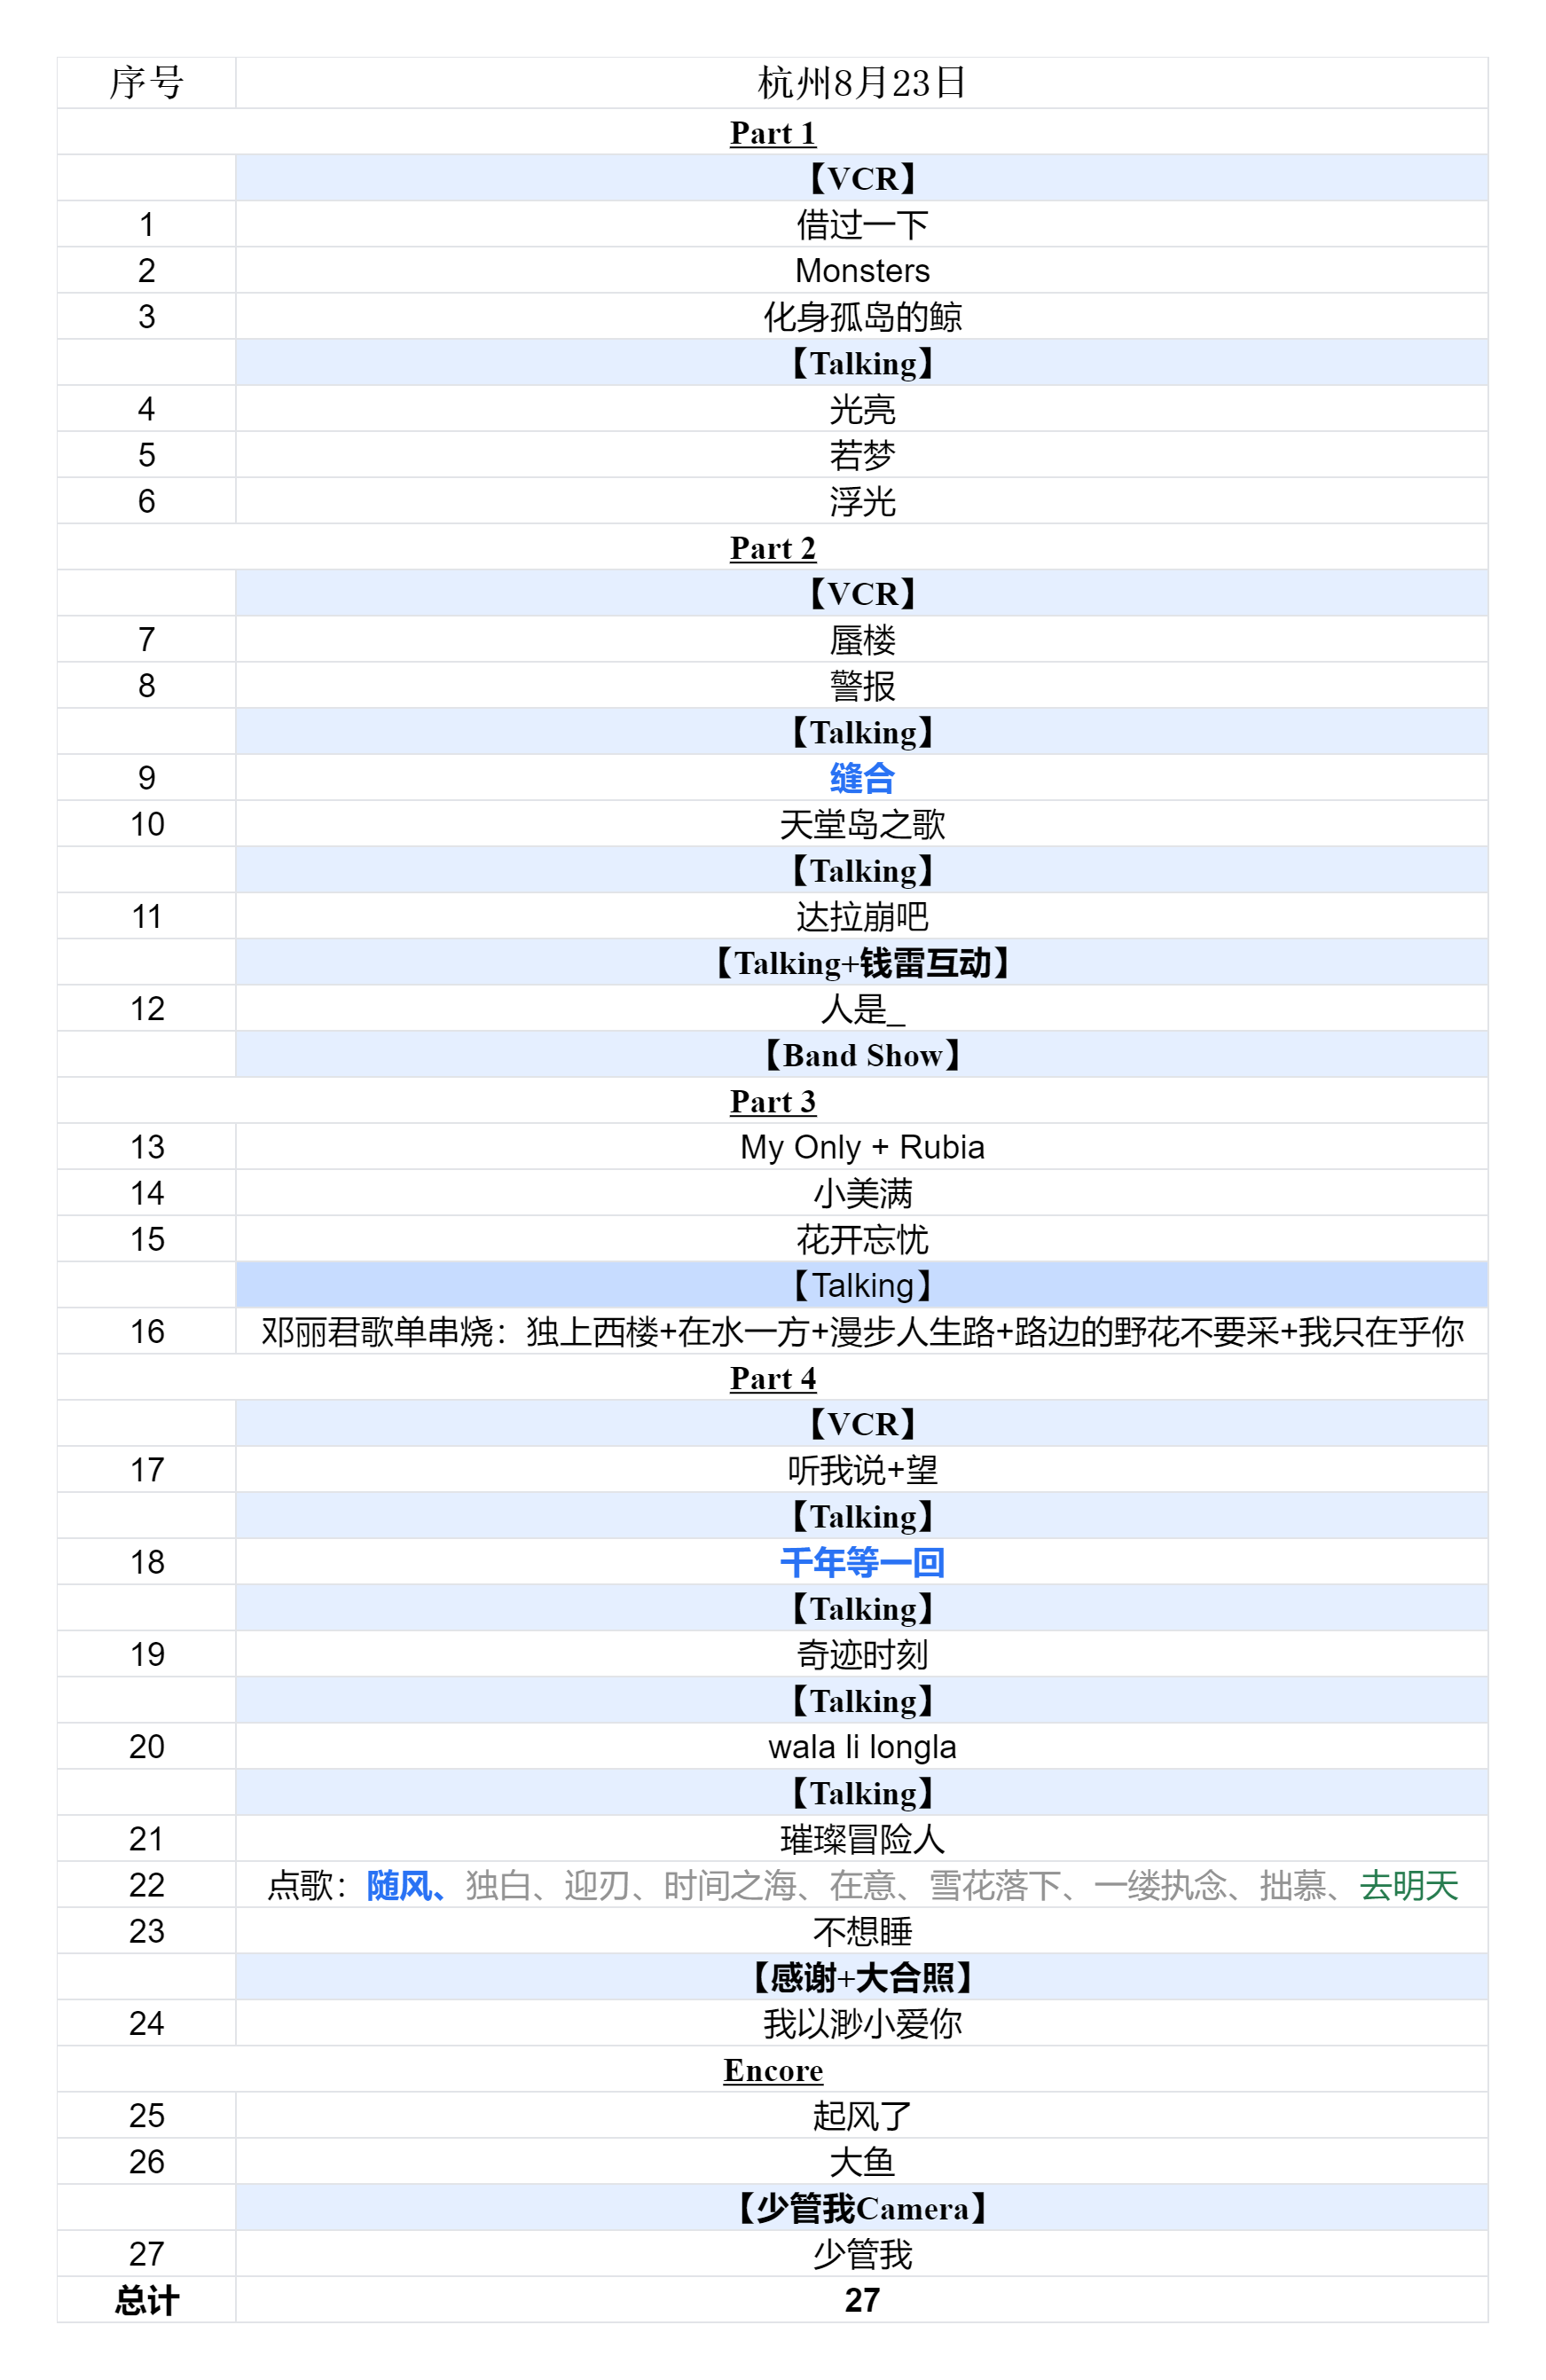
\includegraphics[width=320pt]{img/playlists/playlists-hangzhou-20240823} 

}

\caption{2024周深9.29Hz巡回演唱会2024.08.23杭州场歌单}\label{fig:unnamed-chunk-80}
\end{figure}

\newpage

\section{Part1}\label{hangzhou-20240823-part1}

\hyperref[opening-vcr]{🎥【\textbf{开场VCR}】}

\hyperref[I-will-go-my-way]{🎵【\textbf{借过一下}】}杭州的朋友们,你们好吗?

\hyperref[Monsters]{🎵【\textbf{Monsters}】}

\hyperref[hua-shen-gu-dao-de-jing]{🎵【\textbf{化身孤岛的鲸}】}这首歌你们愿意跟我一起唱吗?你们\textasciitilde 看台的朋友大声点哦\textasciitilde 到你们哦\textasciitilde 看台的\textasciitilde(没有墙头)我不相信\textasciitilde{}

  杭州的朋友们你们好,大莲花我们来啦\textasciitilde 我想想,我学了一句的,杭州的朋友们大家好,你们吃过了吗?你们辛苦了(杭州话)谢谢大家,大家好我是歌手周深,你们好吗?我们的演唱会主题叫做9.29Hz,曾经我也觉得自己特别像是9.29Hz这样的频率,没有办法被听到,但是谢谢每一个你,你们听到了我,看到了我,谢谢你们,所以如果你也觉得和我之前想法很像,自己也是没有办法被听到的话,那么我想告诉你,你不会孤单的,因为我会听到你们\textasciitilde{}
好,那接下来这首歌,我觉得就自己在,很多时候就自己在事业道路上,或者是在寻找更好的自己的那个路上,有时会觉得很孤单,会甚至有时觉得路上有点黑,但是因为你们的出现,照亮了我的路,因为你们是我的光亮,谢谢你们\textasciitilde 然后今天这首光亮也有我们新的,这算是老朋友了吧,大家掌声欢迎钱雷老师,我给你个机会给大家打招呼。(钱雷:杭州的朋友们大家好,我是现代人钱雷)啥,雷哥其实一直住在杭州,那你会说几句杭州话吗?(钱雷:不会)音乐人是比较直接和诚实的,好,那我们一起把这首光亮送给大家,你们都说我治愈了你们,其实你们才是治愈我的那个人,谢谢你们给我的光亮,谢谢\textasciitilde{}

\hyperref[silver-linings]{🎵【\textbf{光亮}】}你们好吗?谢谢每个看到我听到我的人,你们照亮了我的全部,谢谢大家,也谢谢雷哥,掌声给雷哥\textasciitilde{}
宝你个头!

\hyperref[ruomeng]{🎵【\textbf{若梦}】}等下要跟我一起唱哦\textasciitilde 到你们哦\textasciitilde 看台的朋友,大声点\textasciitilde 谢谢你们,太好听啦\textasciitilde 到你们哦\textasciitilde 全场一起\textasciitilde 大声点\textasciitilde 你们唱的太好听啦\textasciitilde{}

\hyperref[floating-light]{🎵【\textbf{浮光}】}这首歌会跟我一起唱吗?(会)那等下要唱大声点哦\textasciitilde 到你们\textasciitilde 谢谢在这恍惚三万天当中,你们看见了我,听到了我,谢谢大家,我是歌手周深\textasciitilde{}

\section{Part2}\label{hangzhou-20240823-part2}

\hyperref[senself-vcr]{🎥【\textbf{反深代词VCR}】}

\hyperref[mirage]{🎵【\textbf{蜃楼}】}

\hyperref[the-giver]{🎵【\textbf{警报}】}掌声给我们的舞蹈老师们\textasciitilde{}

  大家好,我是歌手周深,你们好吗?杭州的朋友们你们好吗?看台的朋友你们听到了吗?这边的朋友你们好吗?我听说,就是听说哦,我也从来没有这样体验过,就是在演唱会,手指到哪里哪里就会有欢呼声,是真的吗?这边呢,这边呢,那看台的那边会有吗,这边呢,那如果是这样呢?哇塞,你们太棒了,给自己鼓掌\textasciitilde 谢谢大家,谢谢你们给我安全感,让我愿意去把新的周深的一面去介绍给大家,前面第一部分比较古风飘渺的是比较大家熟悉的周深,刚才演唱的是新专辑反深代词,反深代词的深是周深的那个深,我记住了\textasciitilde 反深代词的新歌第一个蜃楼写的执念,警报写的是要好好爱自己,那今天要唱的这首歌叫做缝合,我觉得自己很幸运可以成为一个歌手,因为这特别像这首歌里面写的200年后的缝合机器人一样,他可以不停的去缝我们人类受到的创伤,无论是小的时候还是长大之后,虽然他的这个缝合或者是我的歌声,不会把所有的伤口缝补得像伤害从来没有来过一样,但是其实很多时候我会发现,你们才是那个用爱去缝合我的人,所以我觉得特别特别幸福,哪怕我们所有的缝合这个动作,他不会让那些伤害消失,不会让那些伤害像没有来过一样,但正是因为我们互相用爱去缝合彼此,这就是缝合的意义,谢谢你们。真的非常荣幸能够出现在大家生命当中,谢谢你们听见了我,我们继续用爱缝合彼此好吗?

\hyperref[fix-you]{🎵【\textbf{缝合}】}好好的爱自己,你们没有必要做到完美,没有必要做到100分,\textbf{\textcolor{red}{我爱你们~} }

\hyperref[haven-song]{🎵【\textbf{天堂岛之歌}】}谢谢老师们\textasciitilde{}

  糟糕糟糕,爱你们这件事,我逃不出去啦,哪怕你们墙头这么多,(没有)没有吗?那边的也没有吗?那边的也没有吗?连看台的也没有吗?那我就要考验一下,有一个童话故事,那个主角的名字叫做?人多就是有个好处,哪怕你们背错了我也听不出来,看台的朋友再来一遍,达拉崩吧\textasciitilde 哦,那全场他打败的那条巨龙叫做?哇塞,有点厉害哦,杭州的朋友们非常棒哦\textasciitilde 杭州的朋友们,那这首歌我们一起来再想想,到底是谁为了拯救谁,然后打败了谁,他们回到了哪里,好吗?也希望我们都能拥有童话般的浪漫\textasciitilde{}

\hyperref[dalabengba]{🎵【\textbf{达拉崩吧}】}看台的朋友\textasciitilde 杭州的朋友们,到你们了哦\textasciitilde 到底是谁拯救谁,打败谁,又回到哪里呢?准备好了吗?于是\textasciitilde 砍向\textasciitilde 然后\textasciitilde 咬了\textasciitilde 最后\textasciitilde 恭喜我们成功啦\textasciitilde{}

  谢谢大家,非常非常开心,能够用很多形式让大家看见,比如像是奔跑吧里面活泼的我,然后也像是电影、或电视剧OST里的我,大家都有从这些途径看到我嘛?那要说到写歌非常好听的人,大家一定会想到?你们情商着急啊,刚才才请完人家钱雷老师,重新来一下,呀,我们都当刚没发生过,321,哎呀,如果要说写歌写得非常好听,我们一定要提到?掌声欢迎他,他又来啦\textasciitilde 这么内向,大家提到钱雷老师,第一个会提到什么歌?应该是,爱你孤身走暗巷\textasciitilde 雷哥,这次要好好跟大家打招呼,正儿八经的打招呼\textasciitilde(钱雷:大家好,我是反深代词的,呃,制作人)那,我想问一个,你写歌的时候有没有想过,自己是不是人这个问题\textasciitilde(钱雷:我是手机)哈哈哈,因为雷哥写的歌都太难了,所以当时为什么要把歌写那么难?(钱雷:因为你能表达的非常好,你要是唱不上去,我也不带那么写的)那我只能说,把歌写的这么难,我就是很有压力连开什么三四五场,都是雷哥背的锅,那大家要是找你的话,你会怎么说?(钱雷:找我????)好了,音乐人最擅长的就是用音乐跟大家对话,希望大家喜欢这首歌,人是\_,是人吗,写那么难?

\hyperref[renshi]{🎵【\textbf{人是\_}】}大声点\textasciitilde 我们一起\textasciitilde 大声点\textasciitilde 掌声给钱雷老师,谢谢你们,太棒啦\textasciitilde{}

\section{Part3}\label{hangzhou-20240823-part3}

  Hello hello大家好,你们找得到我在哪吗?我在这里\textasciitilde 杭州的朋友们你们好!接下来要演唱的歌都非常的浪漫和温馨,甚至浪漫到我们的舞台只转过来一半,就想看下你们岂不期待我的出现啊?谢谢你们,如果说,就是相遇是\textasciitilde 我觉得所有的话都在接下来两首歌中,希望你们能喜欢这两首歌好吗?我也老大不小了,学一个新的技能我也很开心,但是希望你们能够给我鼓励好吗?也想告诉你,想学一个事情,任何时候都不晚,记住了吗?

\hyperref[my-only]{🎵【\textbf{My Only}】}\hyperref[rubia]{🎵【\textbf{Rubia}】}你一定要记住你们是点亮我的每一束光好吗?也谢谢你们,愿意接住我的每一个碎片,哪怕那个碎片它不完美,甚至说是有一些缺点,但是谢谢你们接住了我,谢谢你们\textasciitilde{}
接下来这首歌,你们要跟我大合唱好吗?那它是什么歌呢?

\begin{figure}

{\centering 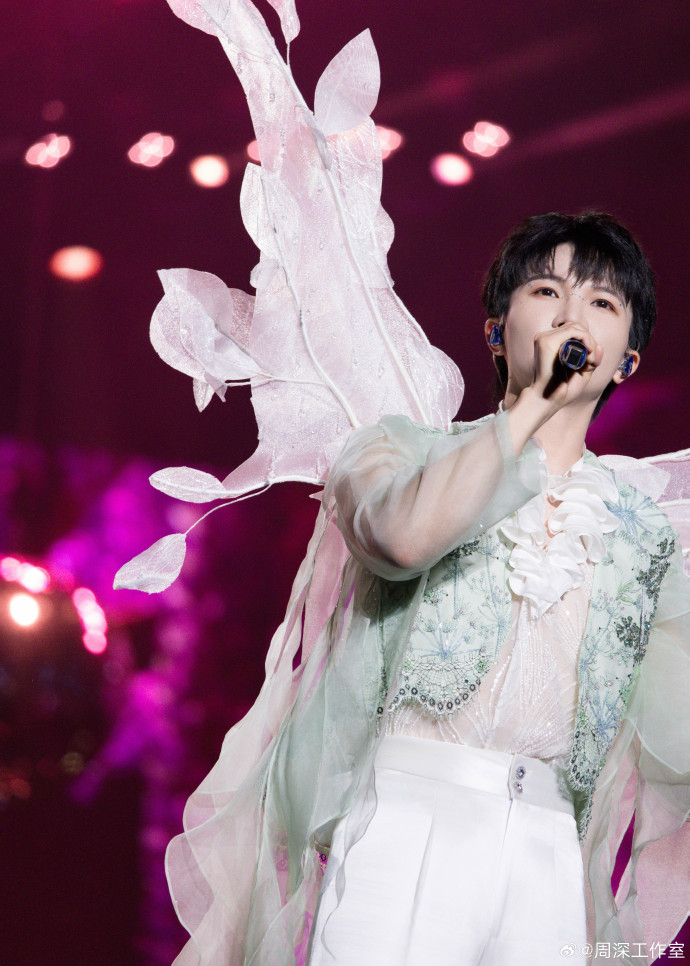
\includegraphics[width=450pt]{img/hangzhou20240823/001} 

}

\caption{绝美瞬间!【@weibo-charlie-studio】}\label{fig:unnamed-chunk-81}
\end{figure}

\hyperref[happy-ending]{🎵【\textbf{小美满}】}会唱吗?那要跟我一起唱吗?看台的朋友大声点哦\textasciitilde 全场\textasciitilde 你们太棒啦,你们的版本真的太好听啦\textasciitilde 再大声一点好吗?大声点哦\textasciitilde 再大声\textasciitilde 谢谢你们,在这个夏天跟我相遇,夏天很快要过去了,但是谢谢你们陪我闯过风,闯过雨,然后我们身上流的每一滴汗,或者说我们创造的每一个记忆,在每一个夏天到来的时候,我都会想起来,谢谢你们给我的这些小美满\textasciitilde 小美满这首歌特别的美好,所以我觉得它特别适合许愿,我们一起在这里许愿好不好?就像我这样,许一个愿望,321,它就会挂在这颗许愿树上,现在我们全场的朋友,跟我一样,闭上眼睛,听话,无论你是做什么职业,什么年纪的,现在闭上眼睛,默默想好那个愿望,默默想好那个愿望,想想你想许什么愿望呢,但是这个愿望有一个要求,就是只能够关于你自己,现在闭上眼睛,想想这个愿望,有多久没有好好的问候一下自己,没有好好的问一下自己,最近过的好吗,想好了吗?321,你们的愿望一定会被听见的\textasciitilde(唱:你们就是周深最好的陪伴\textasciitilde)也希望遇见我这件事情能成为你生活中的小美满好吗?

\hyperref[no-worries]{🎵【\textbf{花开忘忧}】}我来到你们家里啦\textasciitilde 希望大家像小美满里面一样,好好的爱自己好吗?这样爱你的人才不会为你担心,一定要做到哦\textasciitilde 我们一起\textasciitilde(我们苍老的时候,就回到小时候)我们的思念,我们的爱,离开的人一定听得到,对吗?我以前觉得自己喊的不够大声听不到,但是谢谢你们,我觉得他、他们一定都听得到对不对?谢谢\textasciitilde{}

  嘤嘤嘤\textasciitilde 谢谢你们\textasciitilde(换衣服)到底是为什么我换衣服。。。你们,这里有没有谁是第一次来看演唱会的?这么多吗?哦那你们是第一次看演唱会就在这里跟我们一起相遇的吗?哦,谢谢你们,那有没有谁,就是听到,就是第一次听到歌声是听到周深呢?骗子,你出生前,这两位直接哈哈哈哈,难道你们在遇到我之前都没听到歌吗?难道你们就从来没在路边听到哪怕是啊啊啊啊\textasciitilde 的歌吗?骗子,但是这个善意的谎言,我就选择相信一下,哇,原来有这么多人是因为我才喜欢听歌的,谢谢你们\textasciitilde 但是,第一个算是启蒙我唱歌的歌手,她叫邓丽君女士,所以这里有没有人喜欢听她的歌呢?所以我觉得邓女士她每首歌当中都会有很多的时光胶囊,有很多他们的回忆,所以我也希望自己能够成为像一个像邓女士这样的歌手陪伴大家好吗?或者隔了再多再多年,大家还是会想起周深的歌,周深的歌声,但是无论后面怎样,现在我觉得周深非常幸福,因为遇到了你们,你们看见了我,听到了我,谢谢你们\textasciitilde 等下会唱的话跟我一起唱哦\textasciitilde 你们唱得好吗?(好)唱得这么好那你们上来唱?等下跟我一起唱好吗?

🎵【\textbf{邓丽君组曲}】你们太棒啦!摇起你们手中的荧光棒\textasciitilde 到你们唱哦\textasciitilde 看台的朋友也听好哦(路边的野花,你不要采)全场\textasciitilde 大声点\textasciitilde 你们会忘记我吗?谢谢你们\textasciitilde 大声点\textasciitilde 全场一起好吗?不要忘了我好吗?

\section{Part4}\label{hangzhou-20240823-part4}

\hyperref[thank-you-vcr]{🎥【\textbf{谢谢杭州,谢谢你VCR}】}

\begin{figure}

{\centering 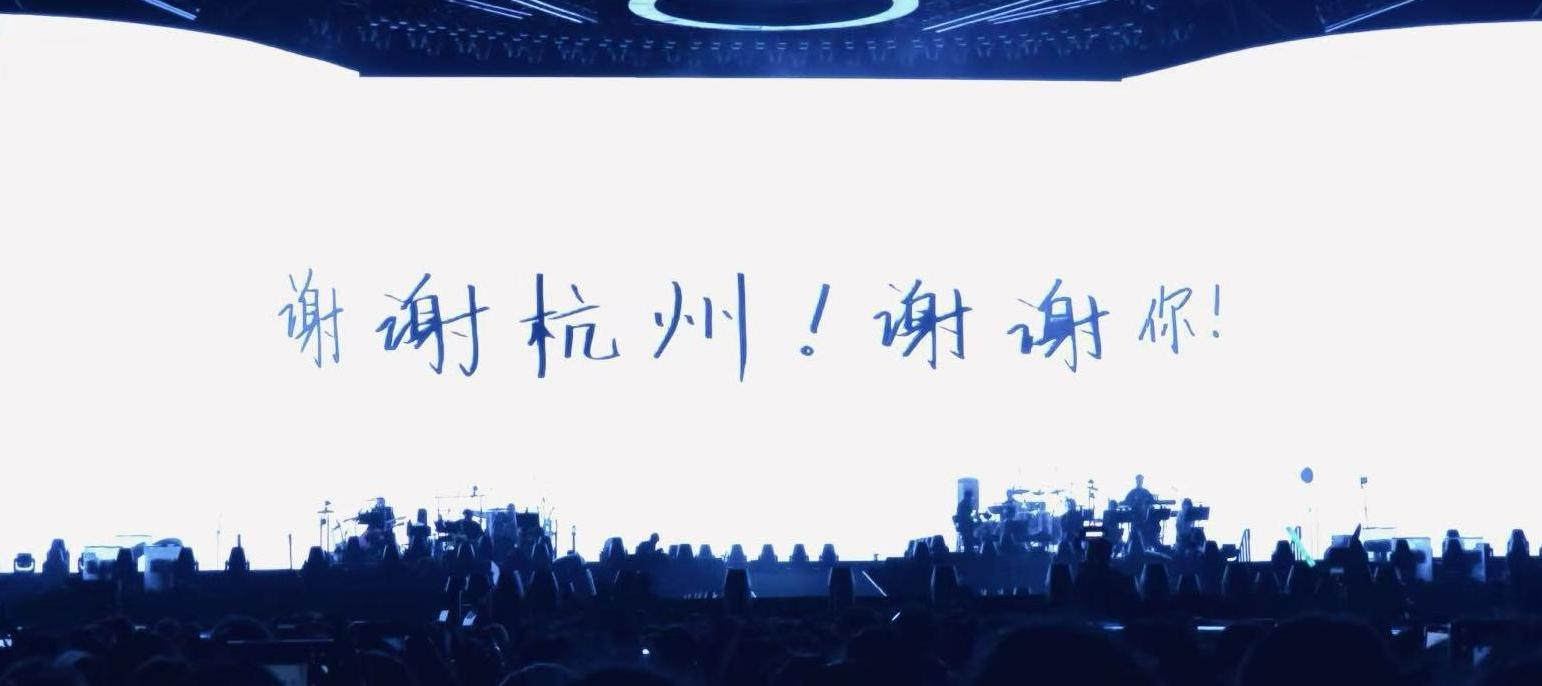
\includegraphics[width=400pt]{img/hangzhou20240823/thank-hangzhou} 

}

\caption{谢谢杭州!谢谢你!}\label{fig:unnamed-chunk-82}
\end{figure}

  大家好,我都听到了哦,爱你个头啊\textasciitilde 宝你个头啊\textasciitilde{}

\hyperref[listen-to-me]{🎵【\textbf{听我说}】} \hyperref[hope]{🎵【\textbf{望}】}大声点,看台的朋友大声点哦\textasciitilde 大家要找我说哦\textasciitilde 我们一起好吗\textasciitilde 看台的朋友大声点\textasciitilde{}

  谢谢你们,兜兜转转,绕啊绕,最后我们还是相遇啦,谢谢你往前迈的每一步\textasciitilde 谢谢你们从来没有放开那根牵着我的线,看台的朋友们,你们好吗?大声点\textasciitilde 因为你你你你\ldots\ldots 你你你的存在,我才心有所住\textasciitilde 无论你在哪(唱:不必害怕孤独)无论你在哪,我都在这,好吗!谢谢你们,你们太棒啦\textasciitilde{}

  杭州的朋友们,你们太棒啦\textasciitilde 要说到杭州,第一个大家想到的是,西湖,以及西湖醋鱼,但是,这是我们外地人,以前我从小就觉得,我真的很想去看下断桥,真的好想去看下西湖,因为有个特别美丽的神话故事,它叫做?(白娘子)被拍成了电视剧,它里面的片头曲,叫做千年(千年等一回),我很开心,我们的相见,我只等了10年,但是我也相信,一定是,就怎么说,我们从当中走的路,绝对也不比他们千年等一回走的少,所以谢谢你们走过来与我相遇,谢谢\textasciitilde 那等一下愿意跟我一起唱这首千年等一回吗?(愿意)等下如果我唱千年等一回,你们要唱(等一回啊啊\textasciitilde)对,这个地方很棒,后面还有个地方,嘿哈嘿,好吗?我们来试一下,嘿哈嘿,唱?看台的朋友我没有听到你们声音哦,嘿哈嘿,唱?(嘿哈嘿)突然声音大到震耳欲聋\textasciitilde 谢谢你们,和我一起唱这首千年等一回吧,因为我们10年才在这里相见,也是非常非常非常难得,谢谢你们,愿意来跟我相遇\textasciitilde{}

\hyperref[once-in-1000]{🎵【\textbf{千年等一回}】}你们是最棒的观众\textasciitilde 来喽\textasciitilde 嘿哈嘿\textasciitilde 这边看台的\textasciitilde 断肠也无怨\textasciitilde Chi Chi na\textasciitilde(PS:China太好听了)看台的朋友\textasciitilde 来了哦\textasciitilde 嘿哈嘿\textasciitilde 大声点\textasciitilde 一起\textasciitilde 你们\textasciitilde 唱\textasciitilde 看台\textasciitilde 大声点\textasciitilde 你们太棒啦,一起\textasciitilde{}

  你们唱得太好听啦,怎么合唱这首歌的时候,比小美满的声音还大呢,我生气了,我走了,哄不好了杭州的朋友们,我走了\textasciitilde 那我可以再试一下吗?(深:没什么大愿望)(米:没有什么事要赶)(深:看见路口红灯)(米:一直闪,它像眨眼的小太阳)谢谢你们,一下就被哄好了,好开心啊\textasciitilde 但是无论怎么样,我觉得就像我玩游戏一样,经常可能打不赢,但是只要我能获得快乐,我总能够赢一把吧。就像我们人生当中尝试很多事情,可能会有挫折,但是不要害怕,它就像可能今天大家会流很多汗,来为我们这次见面,对,扇得很用力,但是,每次一到夏天的时候,我的脑海中的记忆,一定会有这段记忆,对于我来说,是非常美妙的奇迹时刻\textasciitilde{}

\hyperref[magic-moment]{🎵【\textbf{奇迹时刻}】}这是一根红蜡烛\textasciitilde【魔术时间】但是需要你们大声喊出啊\textasciitilde321喊\textasciitilde 还需要你们给我一个掌声好吗\textasciitilde321\textasciitilde 谢谢大家!\textasciitilde{}

  那以前我听过一个快乐的密码叫做Hakuna Matata,有人听过这个嘛?但是在我的新专辑当中,反深代词当中,叫做(wala li longla)看台的朋友知道吗?我们来试一下哦,大家跟着我一起念,wala\textasciitilde wala li\textasciitilde wala li long\textasciitilde wala li longla\textasciitilde 这是一个只要喊出来,你就会永远快乐的密码,记得在心情不好的时候,喊一句,wala li longla\textasciitilde{}

\hyperref[wala-li-longla]{🎵【\textbf{wala li longla}】}看台的朋友\textasciitilde 大家一定要天天开心好不好?那接下来,我们一起念响这个快乐密码好吗?跟我一起哦,54321,wala,wala li,wala li long,wala li longla,看台的,wala,wala li,wala li long,wala li longla,看台的\textasciitilde 你们是最棒的观众\textasciitilde 杭州太棒啦\textasciitilde 掌声给我们的舞蹈老师们\textasciitilde 谢谢你们\textasciitilde{}

  我一直特别想跟你们说的一句话,虽然我说了非常非常多次,但是希望你们永远都能够相信,你们能够让一个普普通通的男孩子慢慢的去接近他的梦想,你们的力量,比你们想象的大的多,听到了吗?看台的朋友你们听到了吗?你们一直说是我照亮了你们,但其实是你们的光一直照在我的身上,让我开始愿意去看清自己,愿意去追逐更好的自己,谢谢你们,也希望我们每一个璀璨冒险人都可以收获属于我们的璀璨,璀璨冒险人,出发吧\textasciitilde{}

\hyperref[adventurers]{🎵【\textbf{璀璨冒险人}】}和我一起\textasciitilde 你们都是自己的英雄,一定要记住好吗?你们\textasciitilde 全场\textasciitilde 谢谢大家,璀璨冒险人们,周深可以做到的,你也一定可以做到!谢谢你们\textasciitilde{}

【\textbf{点歌环节}】那接下来,到我们的点歌环节哦,我的这个歌单非常考验到底听我的歌听了多久,因为它是相对来说,比较宝藏歌单的一些歌曲,但是我相信这些歌会是某一个人他心中的宝藏歌曲,对吗?谢谢谢谢\textasciitilde 那等下我们会全场倒数五个数字,我们的摄像老师拍到谁,就会有请他帮我们点出这首歌好吗?全场跟我一起,我们摄像老师这边,转起来\textasciitilde 全场\textasciitilde54321,停\textasciitilde 啊,在哪,你在哪里?hello,你好,(你好),那有个麦克风,你好漂亮,(谢谢)应该怎么称呼你?(呃,叫我wulala)wulala?你和wala li longla的关系是?(也是一样爱你)现在点起来的人的攻击力越来越强了,爱你个头,(深深宝贝)爱你个头啊,宝你个头,(啊\textasciitilde 开心)你是哪里来的朋友?(我从上海来)上海来的?哦\textasciitilde 谢谢你谢谢你,今天非常非常漂亮。(谢谢\textasciitilde)那有听话每天都照顾好自己吗?(有的呀)有在我们相遇之前好好照顾好自己吗?(有的呀,努力上班,赚钱,来看你演唱会)努力上班,赚钱,然后要先把看我这件事情放在照顾好自己后面,好吗?(当然当然)必须必须好吗?(好的)大家也要这样好吗?(好)听我的歌多少年了?(我算算,四五年吧)四五年,那还挺长,第一次听到我的歌是?(应该是China Voice)哦,就是我刚出道那个舞台是吧?那你对我印象最深的歌曲是?除了大鱼?(沉默)印象不深刻,明白了\textasciitilde(太深刻了,每一首都喜欢,选不出来)啊,这下你之前的犹豫,就已经失败啦\textasciitilde(哎呀,你懂的,我爱你)wu\textasciitilde(宝贝)wulala朋友点歌吧,这些歌有你喜欢的歌吗?怎么会问你旁边的人?你的爱都是假的,耶,我又赢啦!(可是我照顾好自己,我也很爱她)哦,好叻\textasciitilde 啥意思每听懂?哈哈(我照顾好自己嘛,所以我也很爱她,所以我问她喜欢听什么)真棒,我说不过你,我错了,我唱还不行吗?这些歌当中有没有你想听的歌?(我想听随风)哇塞,大家都想听随风嘛?看台的朋友也想听吗?哦\textasciitilde 谢谢wulala,谢谢你,我也很喜欢这首随风,然后希望大家也能喜欢这首歌,也希望大家的烦恼都可以随风被吹走好吗?谢谢,随风,希望你们喜欢\textasciitilde{}

\hyperref[with-wind]{🎵【\textbf{随风}】}你们会唱这首歌吗?(会)那等下要帮我一起唱哦\textasciitilde 跟我一起好吗?谢谢\textasciitilde 谢谢你,无论是从任何一首歌中听到了我,谢谢你看到了我\textasciitilde 这首歌等下要跟我一起唱好吗?

\hyperref[keep-playing]{🎵【\textbf{不想睡}】}这个是当时,这画的样子是我在网上唱卡布的麦克风哦\textasciitilde 看出来了吗?宝你个头啊\textasciitilde 跟我一起哦\textasciitilde 到你们\textasciitilde 看台的朋友大声点哦\textasciitilde{}

  谢谢你,听到了我,看到了我,谢谢你,看到了卡布,看到了歌手周深\textasciitilde 全场跟我一起\textasciitilde 看台的朋友大声点\textasciitilde 希望你们能天天都开心\textasciitilde 谢谢你,大家,大家真的辛苦了,无论你是从哪个地方过来跟我见面,当中一定克服了很多很多困难,也放下了自己很多很多事情,谢谢你愿意把这个时间抽出来与我见面,谢谢你愿意抽出来跟我创造这个美好回忆,谢谢你们\textasciitilde 希望你们今天听的开心,玩的愉快好吗?当然也要感谢所有让我们好好的开心的安全的见面的所有幕后的工作人员对不对?(米:对)谢谢。那我们感谢场地支持杭州滨江奥体运营有限公司,感谢和本次巡演的全程主办北京时代立方文化传播有限公司,感谢我们的杭州承办方,以及杭州协办方也是反深代词的发行华纳音乐。谢谢大家,大家记得听一下我的新专辑反深代词哈,感谢感谢\textasciitilde 也感谢我们的演唱会制作单位必应,感谢总导演周佑洋、庄惟惞,感谢我们的音响总监金少刚老师,大家都知道他吗?我们再一次掌声感谢!感谢我们的音乐总监龙隆,以及我们乐队老师们,还有我们合唱老师们,谢谢。还有我们的特别嘉宾就是雷哥,也感谢我们的舞蹈团队SDT ShowPro。感谢服装团队设计师劳伦斯许工作室,谢谢时装品牌windowsen,感谢我们音响工程南京奥斯泰视听科技有限公司,感谢调音团队悦耳工作,谢谢谢谢,感谢硬体工程北京力超舞台集团,怎么会写一个爆帅如雷啊\textasciitilde 哈哈\textasciitilde 感谢我们的周深工作室的小伙伴们\textasciitilde(啊啊啊\textasciitilde)你们真的太好了,谢谢大家,谢谢大家,我们还会继续努力继续进步,希望能照顾好大家,感谢微博\textasciitilde(倒闭)感谢微博音乐\textasciitilde(倒闭)感谢微博演出\textasciitilde(倒闭)最终还是承担了所有\textasciitilde 感谢美丽的城市杭州。也感谢杭州这座城市所有的职能部门的大力支持,感谢他们保障我们这次演出的顺利进行,也感谢我们志愿者们好不好?感谢现场所有台前幕后的工作人员\textasciitilde{}\textbf{还有最最最重要的重磅嘉宾,就是每一个来自现场的你\textasciitilde{}}包括看台的朋友们谢谢你们来\textasciitilde 刚刚演唱的不想睡是卡布的晚安曲,演唱完后卡布就会下麦,接下来这首歌是周深的晚安曲,叫做我以渺小爱你\textasciitilde{}

  在此之前,我们来大合照吧\textasciitilde 中间的朋友\textasciitilde 我发现后面照片我脑袋会挡住几个人,我尽量就是\textasciitilde321\textasciitilde 好,我们左边这边的朋友\textasciitilde321\textasciitilde 谢谢大家,\textbf{我们抓住了夏天尾巴,一起创造了很多夏天的回忆},谢谢你们\textasciitilde 这边的朋友\textasciitilde321\textasciitilde 还有就是那边的朋友\textasciitilde 好没有默契啊哈哈哈\textasciitilde 好,来喽\textasciitilde321\textasciitilde 然后包括这边一点的哦\textasciitilde321\textasciitilde 那边的朋友\textasciitilde321\textasciitilde{}\textbf{很开心出道十年,我们见面啦\textasciitilde{}}这边哦\textasciitilde321\textasciitilde 这边的朋友,你们好\textasciitilde321\textasciitilde 谢谢我们的摄像老师,再次掌声谢谢每一个你\textasciitilde 接下来这首歌是周深的晚安曲,谢谢你们看到了我,谢谢你们在人群中,再渺小你们都看到了我,也谢谢你们照亮了我,我以渺小爱你,希望你能感受到这份渺小的温暖,好吗?

\hyperref[loving-you-in-my-humble-way]{🎵【\textbf{我以渺小爱你}】}\textbf{不要嫌我的力量不够大哦\textasciitilde 因为你们力量非常强大\textasciitilde 谢谢\textasciitilde 谢谢你们\textasciitilde 我们做到啦\textasciitilde 我会努力在舞台上多唱几年的,好吗?\textasciitilde 谢谢你们\textasciitilde 我们一定会再次相遇的\textasciitilde{}}

\section{Part5}\label{hangzhou-20240823-part5}

\hyperref[the-wind-rises]{🎵【\textbf{起风了}】}大家好,我是歌手周深,谢谢你们还在\textasciitilde 你们好吗\textasciitilde 谢谢你们\textasciitilde 谢谢你们,用爱吹起了这阵风,谢谢你们\textasciitilde 谢谢\textasciitilde{}

\hyperref[big-fish]{🎵【\textbf{大鱼}】}(唱:倒流回最初的相遇\textasciitilde)我们相遇啦\textasciitilde 谢谢大家\textasciitilde{}

  还想耽误大家一点时间唱一首专辑里的歌好吗?在唱这首歌之前呢我们会有个少管我的互动,大家知道吗?大家听过这首歌吗?我们试一下哦\textasciitilde 嘿(少管我【无手势?】),如果这也算听过的话\textasciitilde 哈哈\textasciitilde 我们有一个少管我的特定姿势,嘿,少管我\textasciitilde 但是做这个动作的时候小心不要打到前面的头,看台的朋友记住这个动作了吗?来我们全场来一下哦\textasciitilde 嘿,少管我\textasciitilde 没错,少管我这三个字呢,是让大家以一个乐观的心态去看待所有问题,不要争吵不要争执,这些都是很多对少管我三个字的刻板印象,所以我希望我们可以,就是看待所有烦心事的时候都有一个更乐观心态去看待它,就轻轻的说一句,嘿少管我,然后自己对自己负责,去向那个更好的自己向前出发好吗?一样的,全场倒数5个数字,如果摄像机捕捉到你的话,就要喊出你最大音量喊出这句嘿少管我这几个字让全场都能听到好吗?全场倒数五个数字,54321\textasciitilde 啊啊啊\textasciitilde 这是在哪里\textasciitilde(唱:在哪里\textasciitilde)hello\textasciitilde 你手拿着他是怎么想的,你喊出的是少管我这三个字是吗?应该怎么称呼你?布?布星星?星星?就是星星?你是哪里来的?宁波来的?掌声欢迎宁波的朋友来杭州玩\textasciitilde 你什么时候听我唱歌的啊?大概几年前?几几年?四年前?十年前?后边的朋友厉害了\textasciitilde 四年前,你第一次听我的歌是?没想到有这么难的题目吧?还对了,你好意思说\textasciitilde 那就用声音喊出最大声音跟我说少管我\textasciitilde321\textasciitilde 棒棒棒\textasciitilde 谢谢你\textasciitilde 谢谢星星\textasciitilde 我们再来一位吧,全场\textasciitilde54321\textasciitilde 停\textasciitilde 哎呦\textasciitilde hello?你拍我的时候开美颜了吗?应该怎么?前面后面?哦,是后面那位,对不起\textasciitilde 应该怎么称呼你\textasciitilde(生米)生米\textasciitilde 你是聪明的\textasciitilde 那你要代替全场喊出最大声这声少管我哦,好,321\textasciitilde(少管我)特别棒,我们全场再来一次,好\textasciitilde321\textasciitilde 看台的声音大一点,再来一次,321\textasciitilde 谢谢你们\textasciitilde 向更好的自己出发吧\textasciitilde 芜湖\textasciitilde{}

\hyperref[watch-ur-manners]{🎵【\textbf{少管我}】}希望大家能够喜欢新专辑反深代词\textasciitilde 全场\textasciitilde 全场,321\textasciitilde(嘿,少管我)太棒啦\textasciitilde 杭州的朋友,你们太棒啦\textasciitilde 全场\textasciitilde 全场,321\textasciitilde 谢谢你们来看我\textasciitilde 谢谢\textasciitilde 谢谢你\textasciitilde 东西不要掉了好吗\textasciitilde 谢谢你们\textasciitilde 我们一定会再次相遇的对不对?54321\textasciitilde{}\textbf{\textcolor{red}{我爱你们~} } 手机不要掉了,证件不要掉了,好好照顾好自己\textasciitilde{}\textbf{我们在这里发射出的光线,在宇宙另一端还会再次相遇的,所以这次的相遇并不是结束,好好照顾好自己\textasciitilde{}}谢谢\textasciitilde54321\textasciitilde 谢谢你们\textasciitilde54321\textasciitilde 让我们下次相遇之前,好好照顾好自己,ByeBye\textasciitilde{}

\chapter{2024.08.24杭州场}\label{hangzhou-20240824}

\begin{quote}
\textbf{\emph{谢谢你,愿意抓着那根牵着我的的线。------ 周深}}
\end{quote}

\begin{figure}

{\centering 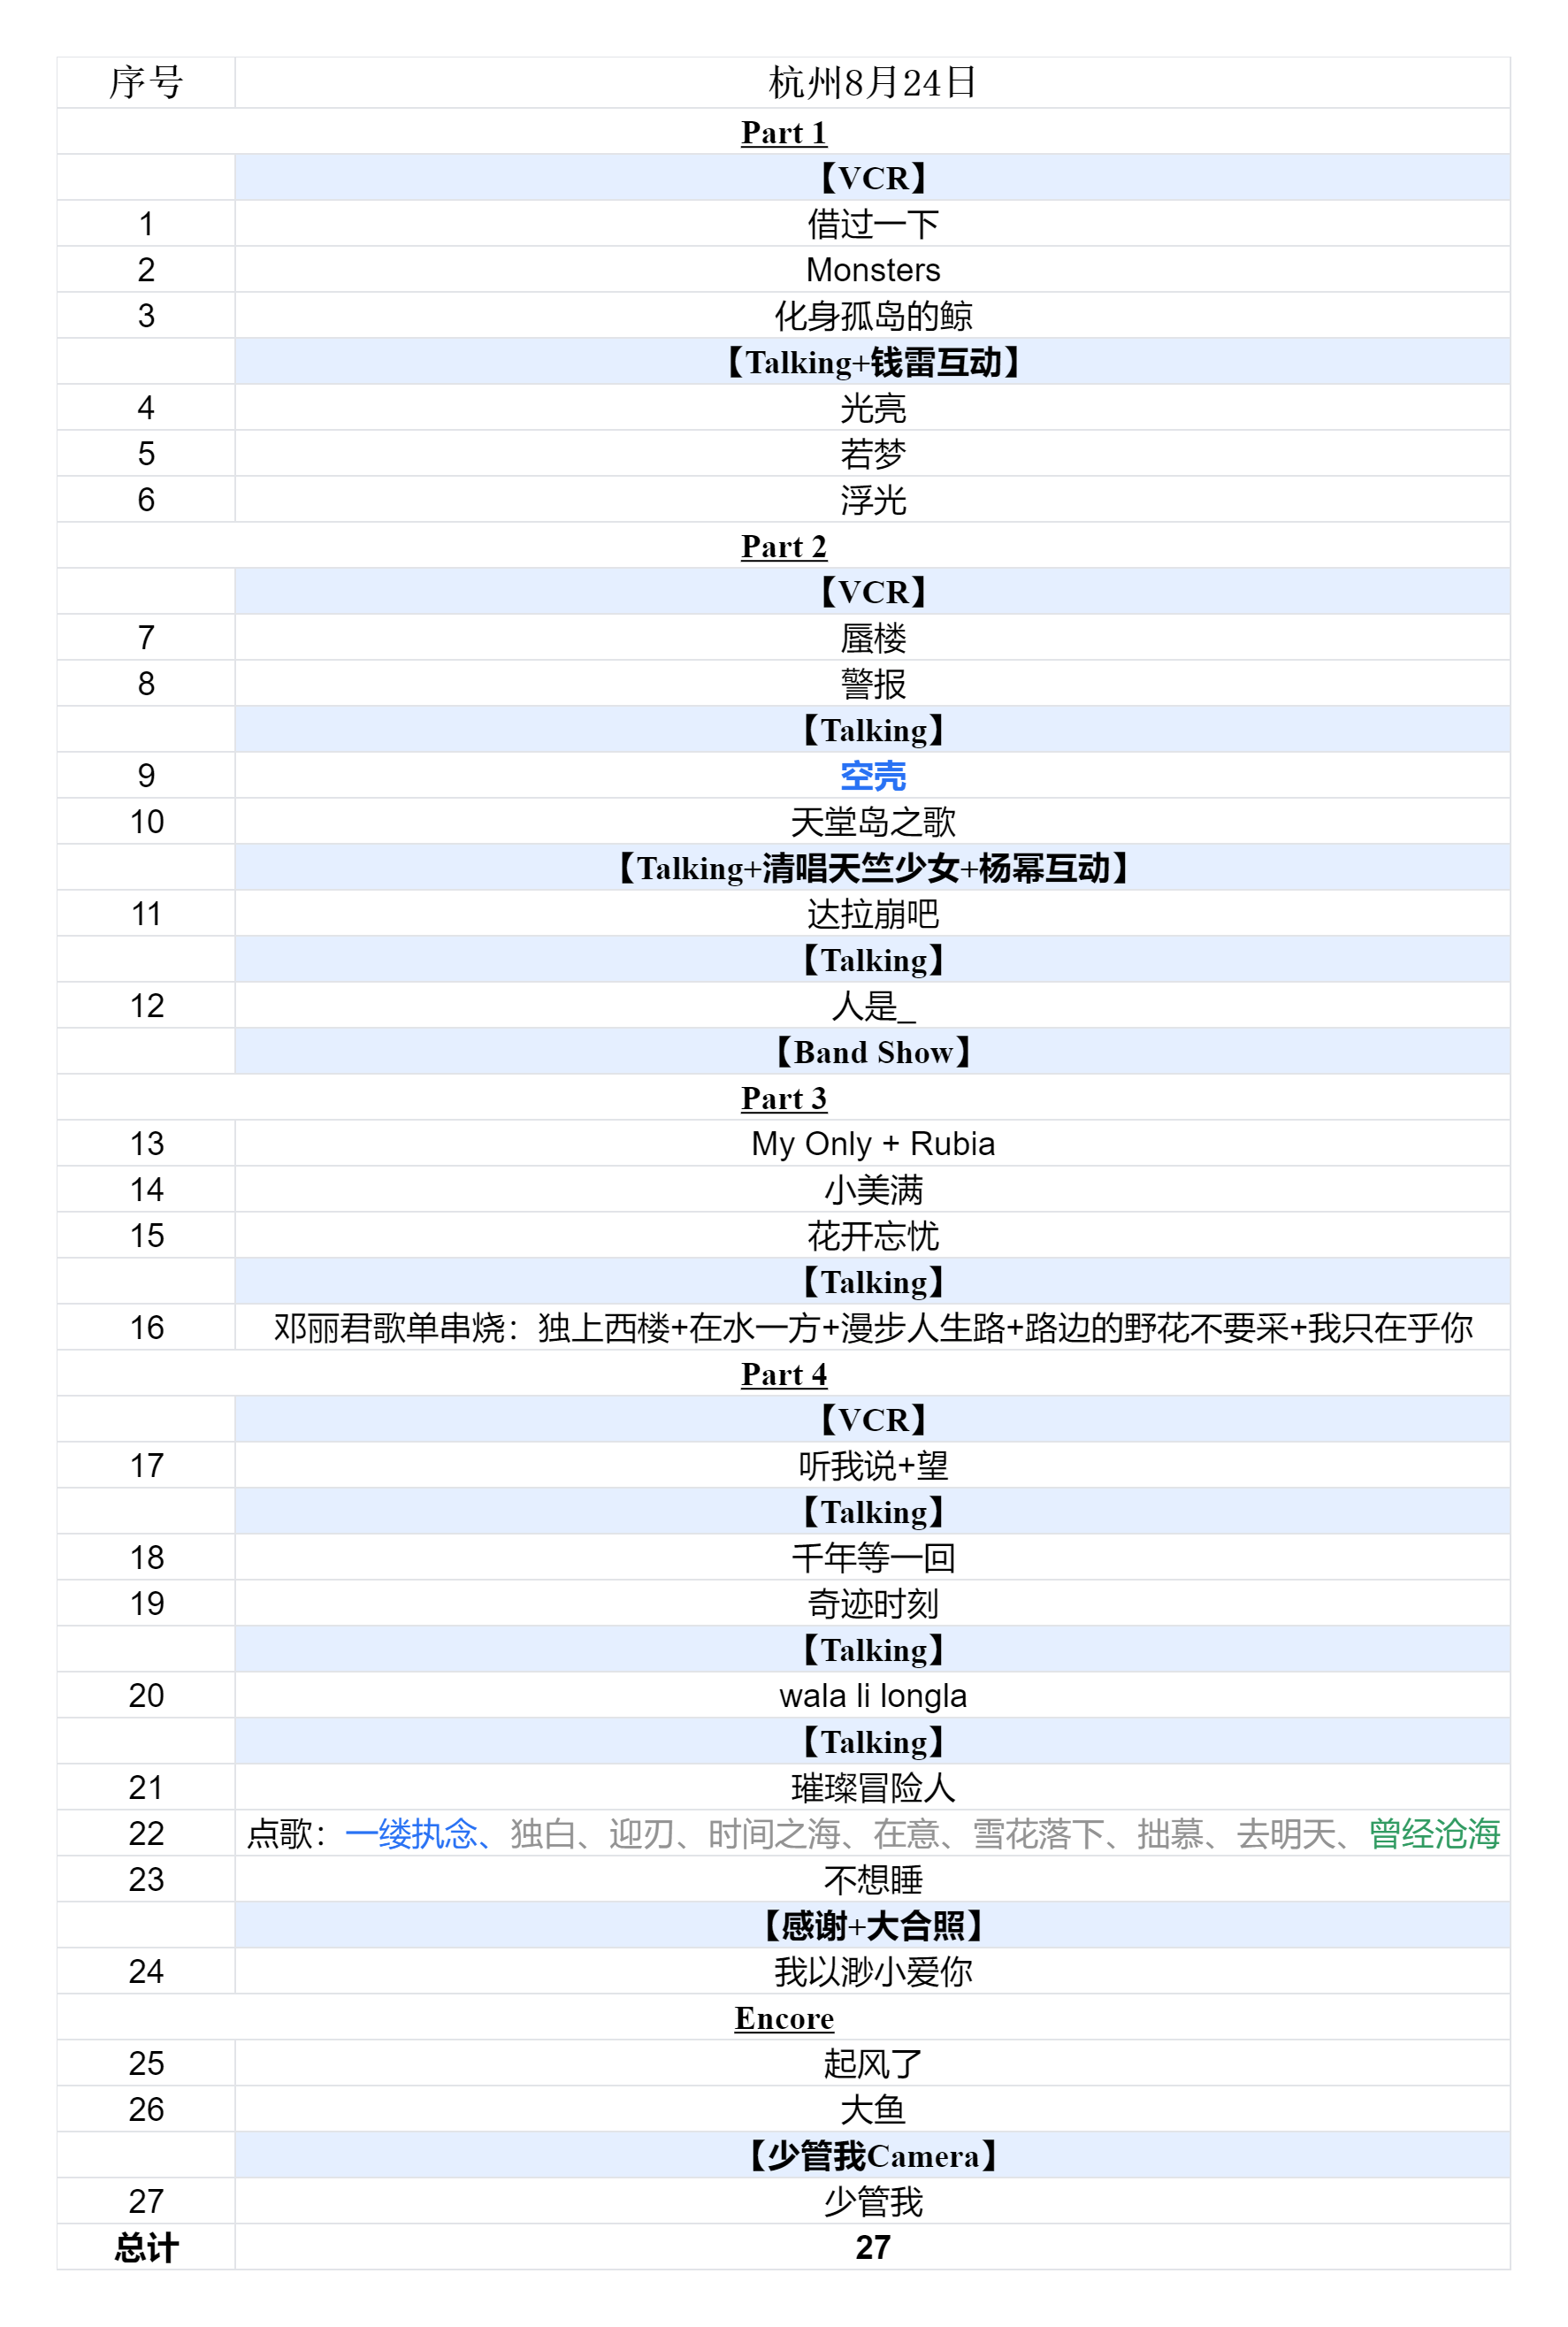
\includegraphics[width=320pt]{img/playlists/playlists-hangzhou-20240824} 

}

\caption{2024周深9.29Hz巡回演唱会2024.08.24杭州场歌单}\label{fig:unnamed-chunk-84}
\end{figure}

\newpage

\section{Part1}\label{hangzhou-20240824-part1}

\hyperref[opening-vcr]{🎥【\textbf{开场VCR}】}

\hyperref[I-will-go-my-way]{🎵【\textbf{借过一下}】}杭州的朋友们,你们好吗?\textbf{你们就是我要寻找的月亮!}

\hyperref[Monsters]{🎵【\textbf{Monsters}】}

\hyperref[hua-shen-gu-dao-de-jing]{🎵【\textbf{化身孤岛的鲸}】}

  杭州的朋友们,你们好吗?(好)谢谢你们,让我这只孤岛的鲸不再孤单。你们愿意跟我一起唱吗?(愿意)谢谢你们\textasciitilde 到你们\textasciitilde 看台的大声点哦\textasciitilde{}
杭州的朋友你们好\textasciitilde 看台的朋友们,你们好吗?(好)。生米们在吗?(在)。谢谢你们,当然今天也有很多很多人来到这一次聚会,我非常开心,无论你是不是生米或者是不是布丁,但是只要你听过我,然后记住了我,然后还选择来到这里跟我一起聚会,就非常感谢你把你的光照到我的身上,谢谢在座的每一位\textasciitilde 巡演的主题叫做9.29Hz。没错,我因为我觉得自己一直都很像是9.29Hz这样的频率,没有办法被别人听到,但是在座的每一个你,或者甚至是没有到现场的每一个你,你们都看到了我,听到了我,这是我莫大的荣幸,我每一次开完演唱会,就结束上一场,然后都心中会有四个字突然蹦出来,就是,何德何能,何德何能能够走进你们的生命当中,陪伴你们,但是哪怕是一首歌的时间,半首歌的时间,我都非常荣幸。因为你们身上的光亮全部都照到了我在前行的路上,谢谢你们,让我不再害怕,谢谢你们\textasciitilde{}

  现在有请我们,掌声欢迎我们钱雷老师,我发现了,昨天在跟雷哥聊天的时候,他现在已经开启了就是已读乱回模式。我说雷哥,你写的歌这么难唱,你是人吗?他说我是手机。那雷哥在杭州已经住了多少多久吗?(呃,两年?)两年?那会说一两句杭州话吗?(钱雷:大家好?)杭州的朋友们,这是他得罪的,哈哈,钱雷,哈哈哈,大家对钱雷的名字,的长相可能会陌生,但是雷哥写的很多歌大家肯定不陌生,比如你再多说两句,(钱雷:怕你飞远去\textasciitilde)像孤勇者啊、如愿啊\textasciitilde 人世间,还有很多很多大家特别喜欢的歌都是雷哥写的,当然,大鱼也是雷哥写的哟。接下来这首歌希望你喜欢,也感谢你的光照在我的身上,这首歌叫做光亮\textasciitilde{}

\hyperref[silver-linings]{🎵【\textbf{光亮}】}你好!\textasciitilde 掌声谢谢雷哥\textasciitilde{}
接下来这首歌要跟我一起唱,好吗?(好)因为我觉得你们才是唱的最好听的一个版本。宝你个头,我现在很高冷\textasciitilde{}

\hyperref[ruomeng]{🎵【\textbf{若梦}】}等一下你要唱得跟喊一样大声哦\textasciitilde 看台的朋友一起唱好吗,等下?(好)到你们\textasciitilde 大声点\textasciitilde(米:往事流转,在你眼眸\ldots)太好听啦\textasciitilde 谢谢你们\textasciitilde 大声唱\textasciitilde 看台的朋友大声点\textasciitilde 全场和我一起\textasciitilde(深:因为你们,我才得到拯救)
感谢这人世间的恍惚三万天我们相遇了,谢谢你们\textasciitilde{}

\hyperref[floating-light]{🎵【\textbf{浮光}】}这首愿意跟我们一起唱吗?(愿意)谢谢\textasciitilde 跟我一起\textasciitilde 谢谢这个宇宙让我们相遇啦,谢谢你们,\textbf{\textcolor{red}{我爱你们~} } 谢谢\textasciitilde{}

\section{Part2}\label{hangzhou-20240824-part2}

\hyperref[senself-vcr]{🎥【\textbf{反深代词VCR}】}

\hyperref[mirage]{🎵【\textbf{蜃楼}】}

\hyperref[the-giver]{🎵【\textbf{警报}】}谢谢\textasciitilde{}

  杭州的朋友们,你们好吗?(好)大莲花我们来啦\textasciitilde 昨天开完第一次大莲花就觉得,哇杭州的朋友们好热情,然后好像昨天试了一下,就是指在哪里,哪里就会有欢呼声,这是真的吗?这边呢,这边的声音会变这么大吗?那如果是指看台的朋友会有吗?那边呢\textasciitilde 那我试一下如果是这样,声音会非常大吗?谢谢大家,大家好,我是歌手周深,你们好吗?(好)刚才我下台换衣服的时候就有人来跟我说,说我们杭州的朋友实在太热情了,热情到我们的荧光棒现在都失控。哈哈哈,大家有没有发现那些荧光棒好像没办法亮,所以我很害怕,就是自己是孤单站在这里,你们在这里听我唱歌吗?(在)谢谢你们,刚才演唱的是我的新专辑反深代词的两首歌,蜃楼说的执念,有好的执念和让自己困扰的执念,第二个警报说的是一定要警报给每一个忘记好好爱自己的人,所以如果你是那个收到警报的人,记得要好好爱自己,前面第一部分是大家比较熟悉的,古风的抒情的周深,也感谢你们给我安全感,让我愿意去把另外一面的周深介绍给你,谢谢你们,也希望我可以给你们这样的安全感,好吗?(好)接下来想耽误大家一点时间,我想唱一首也是新专辑里的歌,这首歌它叫做空壳。那到底什么是空壳?那空壳最后他又获得了什么?或者是失去了什么呢?我相信如果你愿意走进我的世界,一定会明白这一切,谢谢你们,每一个人,到场的人,你们都将我这个感觉像是空壳的人,都让我觉得很充盈,很富有\textasciitilde 谢谢你们\textasciitilde{}

\hyperref[shen]{🎵【\textbf{空壳}】}遇到了你们,发现做一个空壳我也非常的有意义\textasciitilde 也可能因为我是空壳才可以有幸的承载大家很多的情绪,然后慢慢把它放进歌里,所以我是一个收获满满的空壳。很荣幸能够做你的空壳\textasciitilde{}

\hyperref[haven-song]{🎵【\textbf{天堂岛之歌}】}谢谢大家,你们好\textasciitilde 糟糕了,爱你们这件事情我真的逃不出去啦\textasciitilde 那你们会忘记我吗?(不会)哈哈,下面有个人说好吓人,刚才那首歌吓人吗?但是我觉得能够被你们的暖暖的热情包裹我真的好幸福\textasciitilde 谢谢在场的每一个你,谢谢\textasciitilde{}

  然后之前我有个舞台是唱喽天依和言和的一个童话故事,有人知道是什么吗?(达拉崩吧)那我们考一下啊,主人翁的名字叫?(达拉崩吧。。。)大家特别像,大家特别像,就是语文老师在考试的时候,然后说一起背读课文,全班一起读,根本就听不清到底谁背的是对的还是错,哈哈。但是,今天有一个号称她对这首歌非常非常熟悉的好朋友,我们一起来验证一下考考她好不好?那么他是谁呢?(深唱:是谁,送你来到我身边\textasciitilde)(杨幂拿着扇子半遮面)哦\textasciitilde 露出了一双眼睛,(唱:他那闪闪的眼睛眼睛)(半遮面杨幂:Hi)那我就要考一下,主人翁的名字叫做?(半遮面杨幂:是不是达拉崩吧斑得贝迪卜多比鲁翁)非常对,他叫做达啦崩达崩得崩得贝迪卜多比鲁翁,大家掌声欢迎幂姐,谢谢谢谢,谢谢幂姐,你好吗?(杨幂:hello,hi,现场的小朋友们大家好,我是杨幂)其实是一个特别幸福的事情,因为幂姐其实是陪家人来看的,对,我觉得特别感动,因为我也知道很多的歌迷是家人陪着来的,对不对?有可能是爸爸妈妈呀,或者是孩子陪着来的,所以我觉得这是一个,这是不泼冷水的爱,我也非常感谢来到这里每个人,谢谢你们\textasciitilde(杨幂:谢谢大家支持周深)谢谢幂姐,那如果要说,你真的对达拉崩吧熟吗?(杨幂:你起个调吧)来,全场提醒一下?预备,达拉崩吧\textasciitilde(达拉崩吧斑得贝迪卜多比鲁翁)哇,对对对,诶,那幂姐,你觉得我刚才唱得还行吗?(杨幂:沉默片刻\textasciitilde)这么这么长的一段安静的时间,我是有多不行,唱的。(杨幂:少管我)幂姐,你没事吧?(杨幂:您的好友已下线)好友已下线,好,谢谢幂姐,我们掌声给幂姐\textasciitilde 哦对,我觉得,就是我们就是要讲客气,所以必须要回一句,(深唱:我用尽一生一世来将你供养)好,不要再唱了,再唱可能要被打了,哈哈哈\textasciitilde 接下来这首,大家来跟我一起复习,达拉崩吧到底发生了什么好吗?(好)谢谢你们,你们是最棒的\textasciitilde{}

\hyperref[dalabengba]{🎵【\textbf{达拉崩吧}】}摇起你们的双手\textasciitilde 全场的朋友们你们准备好了吗?现在我想听你们跟我说这个童话故事好吗?想想到底是谁为了拯救谁,打败了谁,最后回到了哪里呢?于是\textasciitilde 砍向\textasciitilde 看台的朋友\textasciitilde 然后\textasciitilde 咬了\textasciitilde 最后\textasciitilde 我们来试一下,达拉崩吧\textasciitilde 那么爱念,(唱:要念你来念,吧\textasciitilde)谢谢大家,谢谢\textasciitilde{}

  很奇怪,因为今天刚好因为荧光棒的那个信号,有一些被大家热情热错乱了,反而让我回到了一段我自己小时候在自己长大的那个家乡的一段回忆,我记得是应该是我的亲戚,我忘记是姑妈还是谁,就她会背着我去隔壁村去看,可能隔壁村他们正在表演的那个京剧的一个舞台。因为你们经常说是我把你们带去了一个新的地方,去到新的舞台,但其实一直都是你们在带我去到了新地方,我们从上海出发,然后到深圳,然后到成都,然后再到贵阳,再到武汉,然后再到南京,再到杭州,就每一个地方都是你们,应该是,带我去的地方,我感觉就突然像是你们才是我的那个带我去看世界的那个亲戚,我在你们身上感受到的那一份来自亲情的温暖。所以谢谢你们带我去到越来越大的舞台,我也希望能够陪着你去到你人生当中一个又一个越来越大的舞台。谢谢你们\textasciitilde 也许中途可能会有种种的意外,但是我相信那些都会让它变得更加分。比如像今天的荧光棒可能不亮,但是声音呼喊声会不会更大声呢?(会)雷哥也没有听过咱们现场这么多人一起喊他的名字,我如果喊321一起喊钱雷好不好?321(钱雷)好没礼貌,怎么也不加个老师两个字,哈哈哈,再来一遍,321(钱雷老师)哈哈哈哈\textasciitilde 你怎么感觉跟罚站一样?(钱雷:呃,我想说)你想说,来,说\textasciitilde(钱雷:就是,我记得,做专辑的时候,刚开始)要说这么多句,(钱雷:我跟深深说,我说你帮我录一点奇怪好玩的东西,之后放在我手机里,我跟大家放一放哈\textasciitilde)这个就叫做报复\textasciitilde(钱雷播放深深发的好玩语音:弹舌\textasciitilde 卖萌\textasciitilde)用这首歌送给雷哥,你是人吗?这首歌希望大家喜欢,人是\_,昨天的短裤去哪了?(23号钱雷老师穿着短裤上岗)哈哈哈,希望大家喜欢,人是\_,谢谢你们通过任何一首歌认识我,听到我,谢谢你们愿意选择我,谢谢\textasciitilde{}

\hyperref[renshi]{🎵【\textbf{人是\_}】}现在的钱雷也越来越不好欺负了\textasciitilde 全场,让我听到你们在\textasciitilde 大声点\textasciitilde 看台的朋友\textasciitilde 大家掌声给钱雷老师,雷哥\textasciitilde 谢谢你们,\textbf{\textcolor{red}{我爱你们~} }

\section{Part3}\label{hangzhou-20240824-part3}

  杭州的朋友们,你们好\textasciitilde 看台的朋友你们还在吗?(在)谢谢你们,虽然我现在年纪也老大不小了,但是也学了一个新的一个算小小的新的一个技能,就是弹唱给大家听。希望那时候,肯定弹得不会非常棒,哈哈,希望可以得到你们爱的鼓励,可以吗?也想告诉你,就是如果你想学一个新的事情,他从什么时候开始都不会晚,因为他不需要完美,不需要100分,因为他无论怎么样他都可以收获到同等的快乐,对吗?希望这两首歌也可以温暖的走到你的心中\textasciitilde{}

\hyperref[my-only]{🎵【\textbf{My Only}】}\hyperref[rubia]{🎵【\textbf{Rubia}】}谢谢大家\textasciitilde 谢谢你们\textasciitilde{}

\hyperref[happy-ending]{🎵【\textbf{小美满}】}遇到你们,是我今生最美满的事情,愿意跟我一起唱这首小美满吗?要大声点哦看台的朋友们\textasciitilde 这边\textasciitilde 你们是最棒的\textasciitilde 到你们啦\textasciitilde 看台\textasciitilde 我好幸福啊\textasciitilde 谢谢杭州的朋友,你们都要幸福哦\textasciitilde 让我听到你们\textasciitilde 看台的朋友\textasciitilde{}

  谢谢你们,谢谢你愿意来和我一起抓住夏天的尾巴,从此以后我觉得一到夏天,流掉的每一滴汗,我都会立马想起在场的每一个你,你们是我生命当中最美好的小美满。小美满这首歌非常热闹,让我觉得所有愿望都会实现,我们在这里一起许一个愿吧。我先给大家做一个例子,先闭上眼睛,想好自己的愿望,然后321,噔噔,愿望就会挂在这棵许愿树上,就会被听见,我们努力一定会实现。现在跟我一起闭上眼睛,无论是多大的年纪,或者是做什么职业,现在,闭上眼睛,想好心中那个愿望,想一想最近特别想完成的事情是什么?但是这个愿望有一个条件,就是只能够许关于自己的愿望,想一想有多久没有关心过自己,问过自己有好好照顾自己吗?321,你们愿望都会被听见的\textasciitilde(唱:笑就好,哭也好,你们就是周深最好的陪伴)希望大家像小美满一样,一定时刻要记住好好爱自己,好吗?(好)这样爱你的人他才会放心,才会好好的,更加爱你\textasciitilde{}

\hyperref[no-worries]{🎵【\textbf{花开忘忧}】}说什么?(米:你好啊)你们好啊\textasciitilde 杭州的朋友,我来你们家看你啦\textasciitilde 如果你想念他,就大声地唱出来吧,好吗?花开忘忧,愿你无忧,花开忘忧,(愿你无忧)谢谢大家\textasciitilde{}

  今天还有一个特别感动我的瞬间,就是很多人拿手机打开他们那个手电筒,但是就有的地方,可能一下,唉,这边灭了,可能那个地方灭了,另外一个地方就会亮起来,我在想灭了是不是因为手机太热了?但是,有的时候像这样比较,怎么说呢\textasciitilde(换衣服,全场欢呼)我现在说我很感动的时刻诶\textasciitilde 你在干什么?就有的时候会觉得,好像喜欢听我唱歌的人一直都用这样,有点青涩又略带一些笨拙的爱在包裹着我,我觉得他非常非常的珍贵,谢谢你们,谢谢,谢谢谢谢谢谢谢谢。但是我希望你们不要把手机电量全耗光了,等下要打车回去。好好照顾好自己,好吗?(好)

  我自己第一次听到歌声,应该是听到邓丽君女士的歌声,她对我的影响非常非常大。我也很羡慕邓丽君女士的歌声,感觉只要一想起她的歌声,每个人都会说,啊,你知道吗?那个时候我听,听这首歌的时候在干什么?在干什么?干什么?我也希望我能够成为那样的歌手,说,诶,你知道吗?当时我在听周深那首歌的时候,哎呦,我在做作业,作业做完了吗小朋友?没有?回去要好好做哦,所以我希望自己可以成为这样一个可以一直陪伴大家的歌手,歌手周深会一直加油的,谢谢你们听到我\textasciitilde 谢谢\textasciitilde{}

🎵【\textbf{邓丽君组曲}】
\hyperref[one-in-the-building]{🎵【\textbf{独上西楼}】}(唱:无言独上西楼,宝你个头\textasciitilde)你们好吗?你们好吗?
\hyperref[on-the-water-side]{🎵【\textbf{在水一方}】}到你们\textasciitilde(合:有位佳人,在水一方)你们太棒啦\textasciitilde 掌声给自己\textasciitilde{}
\hyperref[walk-the-road-of-life]{🎵【\textbf{漫步人生路}】}会唱跟我一起,那边的朋友你们好吗?看台的朋友,跟我摇起来你们的双手,没有荧光棒也没有关系,你们正在发光\textasciitilde{}
\hyperref[only-with-me]{🎵【\textbf{路边的野花不要采}】}会唱吗?到你们\textasciitilde(米:路边的野花,你不要踩)我才不会采,但是,你们墙头多\textasciitilde{}
\hyperref[only-you]{🎵【\textbf{我只在乎你}】}你们会忘记我吗?忘了也没关系,因为曾经我们相遇过哦\textasciitilde(深:任时光匆匆流去我只在乎你)你呢(米:心甘情愿感染你的气息)\textasciitilde 大声点,(米:除了你我不能感到一丝丝情意)没错(深:除了你我不能感到一丝丝情意)谢谢每个听过我看到我的人,谢谢你们\textasciitilde{}

\section{Part4}\label{hangzhou-20240824-part4}

\hyperref[thank-you-vcr]{🎥【\textbf{谢谢杭州,谢谢你VCR}】}

\begin{figure}

{\centering 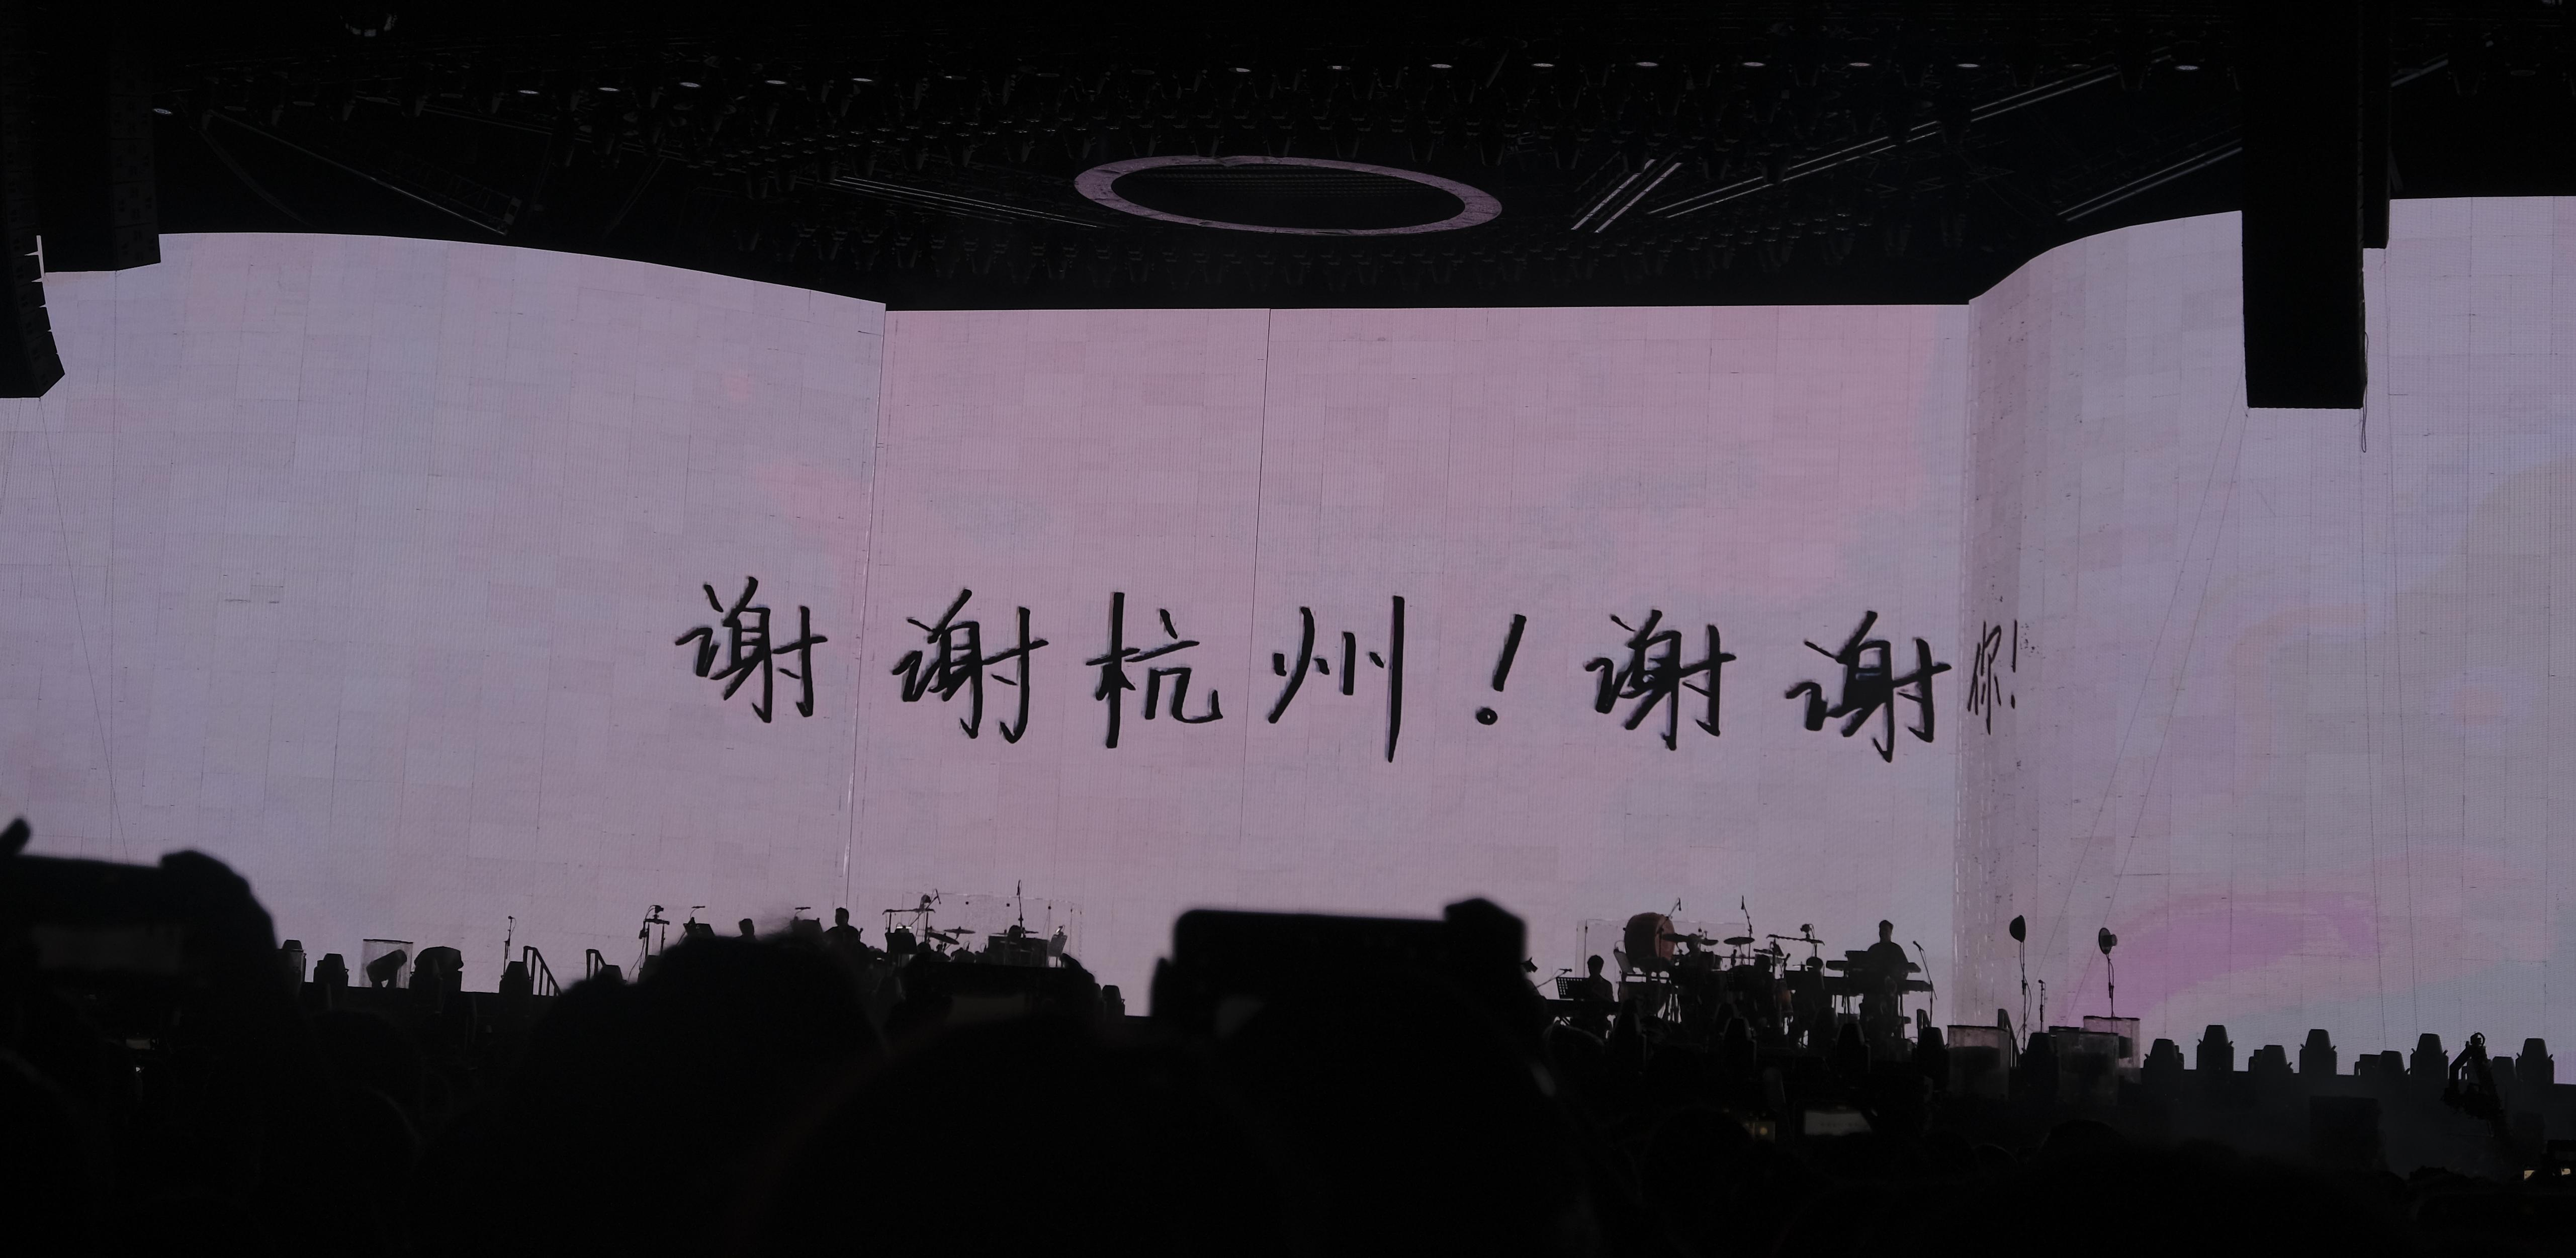
\includegraphics[width=350pt]{img/hangzhou20240824/thank-hangzhou} 

}

\caption{谢谢杭州!谢谢你!}\label{fig:unnamed-chunk-85}
\end{figure}

  杭州的朋友,你们好,你们辛苦了\textasciitilde{}

\hyperref[listen-to-me]{🎵【\textbf{听我说}】}无论你在哪里我都会陪着你们的,跟我一起唱好吗?因为遇到你们日子一定会变好的\textasciitilde 看台的朋友一起唱\textasciitilde(深:开心和难过,总要找个人说说,那个人也可以是我)无论你在任何地方,你都不孤独,你都可以告诉我你的快乐和不快乐,好吗?

\hyperref[hope]{🎵【\textbf{望}】}也谢谢你,愿意抓着那根牵着我的的线\textasciitilde 看台的的朋友,你们听到了吗\textasciitilde 一起\textasciitilde 因为你们,我无论在哪里感觉都像在家里,因为你们,(我才心有所住,你永远都不会孤独)谢谢大家\textasciitilde{}

  非常感谢你们\textasciitilde 我非常喜欢杭州这个地方,因为它特别漂亮而且重要的是杭州的观众真的好热情啊\textasciitilde 谢谢你们带我去到一个又一个地方,谢谢你们让一个普普通通的小男孩子可以慢慢地靠近他的梦想。这是这个男孩子从来没有想过的一个事情,他觉得这一切仿佛都像做梦一样,不会,就是感觉在生命当中不会发生,但是因为遇到你们所有的事情都可以实现。再次感谢每一个看到我听到我的你,谢谢\textasciitilde 今天是我出道的第十年,我们终于在越来越大的地方,越来越热闹的地方,越来越漂亮的地方,相遇啦\textasciitilde 那你们愿意跟我一起唱这一首千年等一回吗?还好我不用等千年,我终于遇到你们啦

\hyperref[once-in-1000]{🎵【\textbf{千年等一回}】}特别棒\textasciitilde 我也无悔\textasciitilde 还有,嘿哈嘿\textasciitilde 全场\textasciitilde 嘿哈嘿\textasciitilde 这边\textasciitilde 到你们\textasciitilde 大声点\textasciitilde(我无悔啊\textasciitilde)我也无悔\textasciitilde 大声点\textasciitilde Chi Chi na\textasciitilde Chi Chi na\textasciitilde(China)Chi Chi na\textasciitilde Chi Chi na\textasciitilde 你们\textasciitilde 看台的朋友大声点\textasciitilde 到你们\textasciitilde 一起\textasciitilde(深:西湖的水)是什么?(米:我的泪)嘿哈嘿\textasciitilde 到你们\textasciitilde 看台跟我一起\textasciitilde 你们是最棒的观众,一起!\textasciitilde 谢谢你们,因为遇到你们,每一秒钟都是奇迹时刻\textasciitilde{}

\hyperref[magic-moment]{🎵【\textbf{奇迹时刻}】}女士们先生们,这是一个白色丝巾,但是,你们321跟我呼唤好么,会发生什么事呢?321\textasciitilde(芜\textasciitilde)哒哒\textasciitilde 还有一个手忙脚乱的魔术,这是一杯牛奶,(喝牛奶)没有问题哦,放在这里,(牛奶杯差点倒了)这是一个罩子,我把它罩住,和我一起321,321\textasciitilde 它就消失啦\textasciitilde 对没错,在这里,但是因为遇到你们,所有的魔术都可以成真。再跟我数一遍321好吗?这是牛奶,给它盖上罩子,321\textasciitilde 它真的,消失啦\textasciitilde 谢谢大家,哎呀\textasciitilde 大家看得开心吗?

  那在反深代词这张专辑当中有一个开心的密码,你们知道是什么吗?(Wala li longla)看台的朋友知道是什么吗?(Wala li longla)我们试一下,我念一遍,你们给我念一遍哦。wala,wala li,wala li long,wala li longla,没错,当你有些许心情烦躁的时候,只要念一下这个密码,所有的快乐都会找到你,好吗?我们全场,再来一遍。wala,wala li longla,希望你们天天都开心\textasciitilde{}

\hyperref[wala-li-longla]{🎵【\textbf{wala li longla}】}摇起你们的双手,让我听到你们\textasciitilde 到你们\textasciitilde 现在全场的朋友要跟我一起念这个快乐密码,好吗?只要你用最大的声音念出来,你就是最开心的那个人,看台的朋友听到了吗?(听到啦)跟我一起来,wala,wala li,wala li long,wala li longla,wala,wala li,wala li long,wala li longla,wala,wala li,wala li long,wala li longla,你们太棒啦\textasciitilde 你们是最棒的观众,谢谢你们\textasciitilde{}

  今天刚好因为看不到荧光棒,我发现一个更可爱的事情。因为我们一起抓住了夏天的尾巴嘛,然后就有看见,有就是``walalilongla!''(挥荧光棒)然后我也有看到就是拿着扇子``walalilongla''(有气无力扇扇子)然后就说用力点他就``walalilongla''(用力扇扇子)。但是我觉得特别好,因为这就是快乐的力量,这就是爱的力量,你们感受到了吗?(感受到了)谢谢,也希望我们每一个璀璨冒险人都可以收获属于我们那个璀璨,好吗?(好)遇到任何困难,不要害怕自己脆弱,我们脆弱是常态,但是我们一定可以创造出属于我们自己的璀璨,对吗?(对)璀璨冒险人们,向前出发吧\textasciitilde{}

\hyperref[adventurers]{🎵【\textbf{璀璨冒险人}】}这位璀璨冒险人,宝你个头\textasciitilde 跟我一起好吗?你们都是自己的英雄,对不对?全场一起\textasciitilde 大声点\textasciitilde(米唱:还想要继续吗?)要\textasciitilde(要炙热啊,要不忘啊)你\textasciitilde(要勇往啊)看台的朋友,你听到了吗?周深可以做到的,你也一定可以做到,谢谢你们\textasciitilde{}

  你们太好了,我突然觉得因为以前我在路边演出的时候,我就在想我一定要努力的唱歌,能够让大家有一个可以遮风挡雨的地方。然后就去到Live house唱歌,然后就发现大家站的特别辛苦,我就想我一定要努力唱歌,能够让大家有一个座位,然后就到了像体育馆或者是一些剧场里面唱歌,然后后面又想,我想让大家就是享受所有天气的浪漫,就发现到了一个就是体育场这个地方,我觉得我们所有的时刻我们全都做到了,所以你们的力量比你们想象中的都要大,千万不要忘记这个事情,好吗?(好)

【\textbf{点歌环节}】那接下来就到了我们的点歌环节,那谁是第一次来听我演唱会的?哇塞,辛苦了,你们好,看台有第一次看我演唱会的吗?所以你们不要高兴的太早,我点歌的歌单相对来说都比较冷,哈哈哈,很有可能你没有听过,但是我相信他一定是某个人的心中他的宝藏歌单,对不对?全场倒数5个数字,然后我们的摄像老师捕捉到谁谁就来帮我们点出杭州场第二站的歌,好不好?(好)谢谢你们,\textbf{你们最好了}。来,54321,停\textasciitilde 您在哪里?您在哪?(在这里)哦,这里,您好,(深深,您好)您好。你嗓门比我还亮耶,你什么时候开演唱会啊?应该怎么称呼您?(我姓佟)佟女士,您好。您好,(深深,您好,我太幸运了),谢谢,谢谢,您是什么时候听我唱歌的呀?(我是,我是第六年了)第六年了,芜,那很长时间了,我才出道10年。那可否问一下您的?就是,啊,不方便,谢谢,(没事没事,我70年的),我对我的冒昧表示抱歉,不对,我觉得特别棒,让我幸福。那您是怎么听到我唱歌的呀?(我是在那个奔跑里你的节目里听到你清唱大鱼)哦,你在跑男里听到我唱歌吗?(对,我的天呐,今天这么幸福)不会不会,那您对我印象最深的除了大鱼还有其他歌吗?可能这个考题会有点难?(每一首),情商真高,但是点歌是我们佟女士的,那您看一下上面有没有您听过的歌,还是说您有什么想跟我说的话呢?(呃,一缕执念)您虽然是,(深深,我还想跟你说,我孙子都喜欢听你唱歌)您孙子,方便透露年龄吗?(今天是我儿子送我过来,因为抢不到票嘛)那儿子在哪里?(回去了)哈哈哈,那等一下,你是自己回去,你是自己来的?(他送我到),你自己是一个人到现场,是吧?(对),谢谢您,所以就是您儿子喜欢听我唱歌吗?(也喜欢,然后我孙子听到你的歌声里会很安静的在那里听,别的事情都不能够让他这么安静,听到你的歌,非常安静的听)谢谢,谢谢,那也就是说您家三代人都喜欢听我唱歌?(对)那还真是,您的孙子是从小听我唱歌长大的,谢谢您,谢谢您,非常非常意外,因为您点的是我第一张专辑里面的一首歌,一缕执念。(深深,谢谢深深)不会,谢谢(我感觉遇到深深以后自己都一路开花了)不会,我就是,我遇到了你们我才发现我的生活越来越明亮,越来越开心,所以跟大家的见面一定是我的一缕执念,谢谢你,(谢谢深深谢谢深深)。哇,您精气神太好了,我希望能够像您这样学习,谢谢佟女士,谢谢,(谢谢深深)。然后这首哦一缕执念,你们想听吗?你们绝对是我的一缕执念\textasciitilde{}

\hyperref[a-wisp-of-obsession]{🎵【\textbf{一缕执念}】}非常感谢你们的存在,让我觉得世界真的太美好啦\textasciitilde 谢谢你\textasciitilde 谢谢我们相遇啦,这个就是一件非常美好的事情,你们也这样觉得吗?(对)

\hyperref[keep-playing]{🎵【\textbf{不想睡}】}跟我一起唱好吗?这边的朋友,你们好吗?你们知道吗?我们在这里发出的光亮在宇宙很远的地方,很多年之后还会相遇,所以哪怕演唱会结束了,我们也会再次遇见的\textasciitilde 到你们\textasciitilde{}

  谢谢杭州场的每一个你\textasciitilde 谢谢,谢谢你们给我造了一个夏天最美的回忆,也希望在你觉得自己心情不好的时候,这个回忆可以时刻拿出来,就像一颗糖一样,给自己一点点甜份,好吗?(好)我们有更好的目标,有更想要成为的自己,但是永远也不要忘记,一颗糖就可以给你带来的快乐,好不好?(好)接下来也要非常感谢所有让我们快乐平安相遇的所有工作人员们,对不对?(对)你们真的太棒了,杭州的朋友,\textbf{\textcolor{red}{我爱你们}}。

  好,那我们感谢杭州市公安局,感谢杭州市消防救援支队,感谢杭州市交警支队,感谢杭州高新区滨江文广旅体局,以及所有职能部门的大力支持,掌声再热烈一点。我非常感谢他们保障我所有的演出顺利进行,也非常感谢我们的场地支持。杭州滨江奥体运营有限公司,感谢本次巡演的全程主办,北京时代立方文化传播有限公司,谢谢你们,谢谢我们的杭州承办方杭州城澳合众文化体育发展有限公司,以及感谢杭州协办方也是反深代词发行公司华纳音乐,大家去听一下我的新专辑好不好?谢谢谢谢谢谢,也感谢演唱会制作单位必应,感谢总导演周佑洋,感谢庄惟惞,感谢音响总监金少刚老师,大家听着我的声音好听吗?(好听),非常感谢金少刚老师,掌声再热烈点。而且金少刚老师每次我们演完他就会说,哇塞,周深,你真的要非常用力的,一定要非常用心的,一定要非常非常多次的感谢你的观众。因为你的观众实在是太优秀啦\textasciitilde 包括看台的,你们听到了吗?你们都是最棒的,一场演唱会,其实你们承载的会更多,所以谢谢你们尽心尽力来跟我们相见,也辛苦你们放下自己的事情,然后用自己的时间来跟我们相遇。真的非常感谢你们,谢谢\textasciitilde 以及感谢我们的音乐总监龙隆老师\textasciitilde 以及感谢乐队老师们,哎呦,还有我们精心打扮的合唱老师们,素贞素贞你怎么在这?(深:青城山下白素贞)后面不记词了啊?对不起,感谢我们的特别来宾,特别老朋友钱雷。感谢舞蹈团队SDT showPro,感谢我们的服装团队设计师劳伦斯·许工作室,感谢时装品牌 Windowsen,以及感谢每一次都非常辛苦帮我们搭建这个舞台,我们一起闯过风、闯过雨,我们跟观众朋友们,也包括他们一起搭建了非常好的舞台理想工程。也感谢我们的调音团队,乐尔工作室,悦不悦耳?(悦耳)谢谢硬体工程北京立超舞台集团,谢谢周深工作室的小伙伴们\textasciitilde 谢谢谢谢,谢谢,大家不要嫌我感谢太多,因为真的还有更多的老师都没有感谢到,很开心我们相遇,感谢微博,(倒闭),我感谢你们\textasciitilde 感谢微博音乐,(倒闭)感谢微博演出,(倒闭)感谢最美的城市杭州,感谢杭州这座城市,感谢现场所有台前幕后的工作人员们,感谢我们的志愿者们,以及最最重要的是,哪怕荧光棒没有信号,但是你们的热情一点都没有减,我,我也看到你们每个人都在,杭州场的每一个你,谢谢你,你你你你你你你你\textasciitilde{}

  我们来大合照吧\textasciitilde 中间,321,左边,321,这边,321\textasciitilde 那边的朋友们,我们来喽\textasciitilde(深:我要奔向你,寻找着生命的意义,哪怕在遥远星海里)这边的朋友,来321,以及再过来一点了,看台的朋友们,321,那边的朋友我来啦\textasciitilde 每次开完演唱会我的步数都要上万,但是我觉得很开心,因为上万步都不及你们靠近我的每一步,321,这边的朋友们,321,谢谢你们。

  刚才的不想睡呢,是以前在网上唱歌的卡布的晚安曲。那接下来要演唱的是歌手周深的晚安曲,我以渺小爱你。

\hyperref[loving-you-in-my-humble-way]{🎵【\textbf{我以渺小爱你}】}谢谢你们在人群当中看到了渺小的我\textasciitilde 谢谢你们给我这一段旅程\textasciitilde 谢谢你们看到了渺小的我\textasciitilde{}
我一直觉得想去的地方就去吧,我可以尽自己的努力,哪怕再渺小,也希望可以去到你家乡,去到你的家里边唱歌,我也不知道自己能够努力地停留在舞台上多久,但是能多唱一首歌,我就多唱一首歌\textasciitilde(深:我以渺小爱你同行的旅程)谢谢你们给我不朽的爱,我很开心,哪怕是一首歌、半首歌、一个副歌陪伴你们,(我以短暂爱你不朽的旅程),只要你听过我,就是那个力量,谢谢你\textasciitilde 谢谢你们\textasciitilde{}

\section{Part5}\label{hangzhou-20240824-part5}

  你们好,谢谢你来,谢谢你还在\textasciitilde{}

\hyperref[the-wind-rises]{🎵【\textbf{起风了}】}谢谢你们\textasciitilde 看台的\textasciitilde 你们好\textasciitilde 谢谢你们,以爱化作风,让我飞起来啦\textasciitilde{}

\hyperref[big-fish]{🎵【\textbf{大鱼}】}

  谢谢你们看到一个歌手叫周深,要相信我这句话,周深可以做到的,你也一定可以,看台的朋友,你们也一样\textasciitilde 因为今天那个荧光棒是没有坏的,但是后面应该是控台信号问题,出了一些问题,所以想给大家小小的说一句,不好意思(米:没关系)所以今天这一场的荧光棒,如果你想拿回去留做纪念的话,是可以带回去的\textasciitilde 那么再耽误大家几分钟的时间,我还想唱一首专辑里面的歌,叫做少管我\textasciitilde 我们会有一个经典动作,希望它成为经典动作,一个指定动作叫做 嘿少管我,全场来试一下,321,嘿少管我(嘿少管我),谢谢,少管我呢,他是一个,就是他不是像看起来一样就让你去争吵或者一定要争个输赢,他是一个以客观或者是乐观的状态去看待所有的问题和不开心的事情,当我们发生发现就很多不开心的事情,你不要去争吵,就发现,只要自己对自己负责,自己知道怎么去成为更好的自己,我们就轻轻地说一句,嘿,少管我,我们就继续轻松前行吧,好不好?(好)

  那这样,全场倒数5个数字,然后我们的相机就捕捉到谁,就要用最大的声音替全场喊出少管我哦,来全场,54321,停,这位戴黑帽子的女生,您在哪里?每次找啊找啊找朋友,可以找半个小时。哦,这里你好,哎呦,应该怎么称呼你?叫你小新。我以为您让我小心,我就说好贴心的朋友,小新,你好,你是来自哪里的?广州的,哦\textasciitilde 那刚才漫步人生路,你有跟着唱吗?(小新:欲摇又点头)要说你诚实呢,你摇了个头,要说你不诚实呢,你后面又点了个头。什么,啊?你不熟悉,你作为一个广东人,好的,那你听我的歌听多久了?十年?哇,这里有没有其他听我的歌听了十年的?(有)你们现在的回应,就像她刚才的第一个反应,那你要用最大的声音喊出少管我,让全场听到哦,好不好?你准备好了吗?准备好了哟,动作,想想,还想,想喊,想喊旁边的小朋友一起呀,你们是一起来的吗?哦,他们是?你的两个宝宝?!芜\textasciitilde 所以后面,谢谢,好,那你们三位,旁边这位不会是?这样子一家子整整齐齐起来,可以少管我好不好?小新女士好幸福,你们怎么这么好,是谁提出先要来看我演唱会的?一起提出?那全家都喜欢我?今天这一场知足了,你们自己玩吧,拜拜,哈哈哈,那全家人要一起喊出最大声音哦,先生怎么称呼啊?小新的先生?好棒,宝宝怎么称呼?小朋友?小小小男孩?啊?小小名应该怎么说呢?给我简单点的,圆圆,哦,小妹妹呢?秘密?Timi?是那个Timi,所以这位先生怎么称呼?好的,你是背后的男人,哈哈哈,全场一起,小朋友们会了吗?嘿,少管我好不好?看来不是很愿意,哈哈哈,321,(嘿,少管我)好没有默契的一家人啊\textasciitilde 哈哈哈,谢谢你们,谢谢来自广东的朋友,谢谢。

  我们全场再来一个倒数,五个数字,54321(猫猫开心转了3个圈圈),停,芜,所以是后面那一位,是吗,应该?这个应该算哪一位啊,老师?摄像老师您摇的人,您来说?那一位?那你把他放大,你觉得是谁来放大,他在这里,好,谢谢,好,我们香港的朋友,好,谢谢,好,就是你了。旁边那个不要再说悄悄话了,说什么呢?好,你好,你在哪?则里?啊,在哪里?在则里?你们都是骗子哦,很远的朋友。你好,怎么称呼你?来帮忙传递一下,来,您的称呼是周女士?钟女士?朱女士?哈哈哈,种女士?周?中?董?彤?彤?什么?钟女士?好的好的,谢谢你,你是来自哪里的?全场就你们听得清,哈哈哈,喊出最大的声音,321,(杭州)杭州的朋友,杭州的盆浴,喊出最大的声音,321\textasciitilde 这个不用传递,我知道他喊的是什么,哈哈哈,再来一遍,321,谢谢,什么女士来着?钟女士,钟女士,谢谢钟女士,我们全场再来一遍,321(嘿少管我)。希望所有的不开心都远离你,爱你们\textasciitilde{}

\hyperref[watch-ur-manners]{🎵【\textbf{少管我}】}谢谢你们还在\textasciitilde 全场一起,全场\textasciitilde 嘿,少管我\textasciitilde 全场\textasciitilde54321\textasciitilde 爱你们\textasciitilde 全场\textasciitilde 全场\textasciitilde54321\textasciitilde 你们是最棒的,谢谢你们\textasciitilde 看台的朋友,谢谢你们\textasciitilde54321\textasciitilde 谢谢你们,看台的朋友\textasciitilde54321\textasciitilde{}\textbf{\textcolor{red}{我爱你们~} } 手机不要掉了,证件不要掉了,你们是最棒的,谢谢\textasciitilde 一定要注意安全,我们会再次相遇的对不对?注意安全,请在我们下一次相遇之前,好好的照顾好自己,好吗?你们太棒啦\textasciitilde 你们答应我的,要好好照顾好自己啊\textasciitilde54321\textasciitilde 谢谢\textasciitilde 谢谢你们让我创造奇迹,也请为自己创造奇迹,byebye,注意安全,手机不要掉了,证件不要掉了\textasciitilde{}

\begin{figure}

{\centering 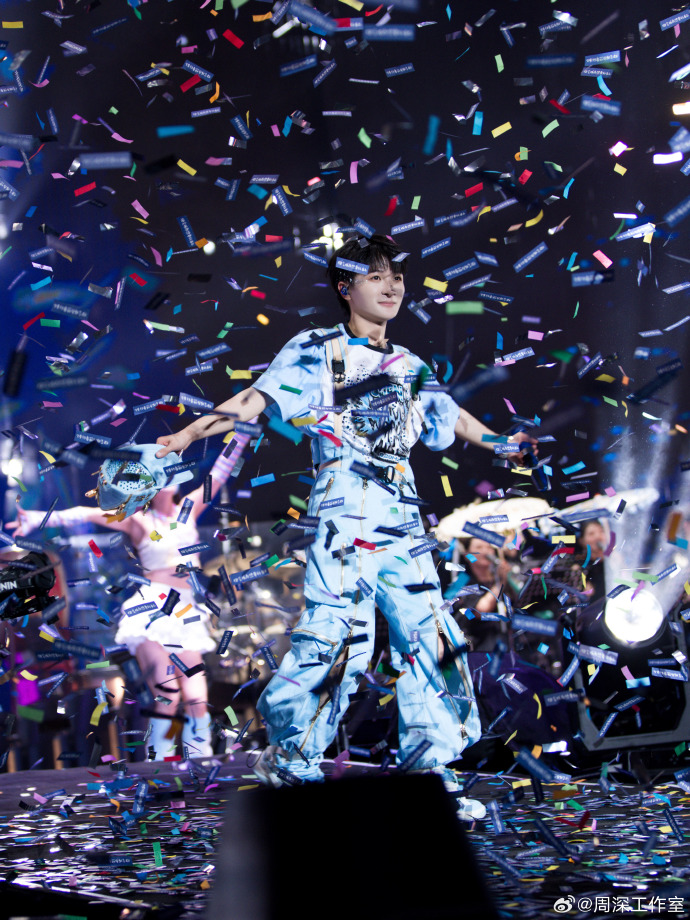
\includegraphics[width=350pt]{img/hangzhou20240824/001} 

}

\caption{绝美瞬间!【@weibo-charlie-studio】}\label{fig:unnamed-chunk-86}
\end{figure}

\begin{center}\rule{0.5\linewidth}{0.5pt}\end{center}

\begin{figure}

{\centering 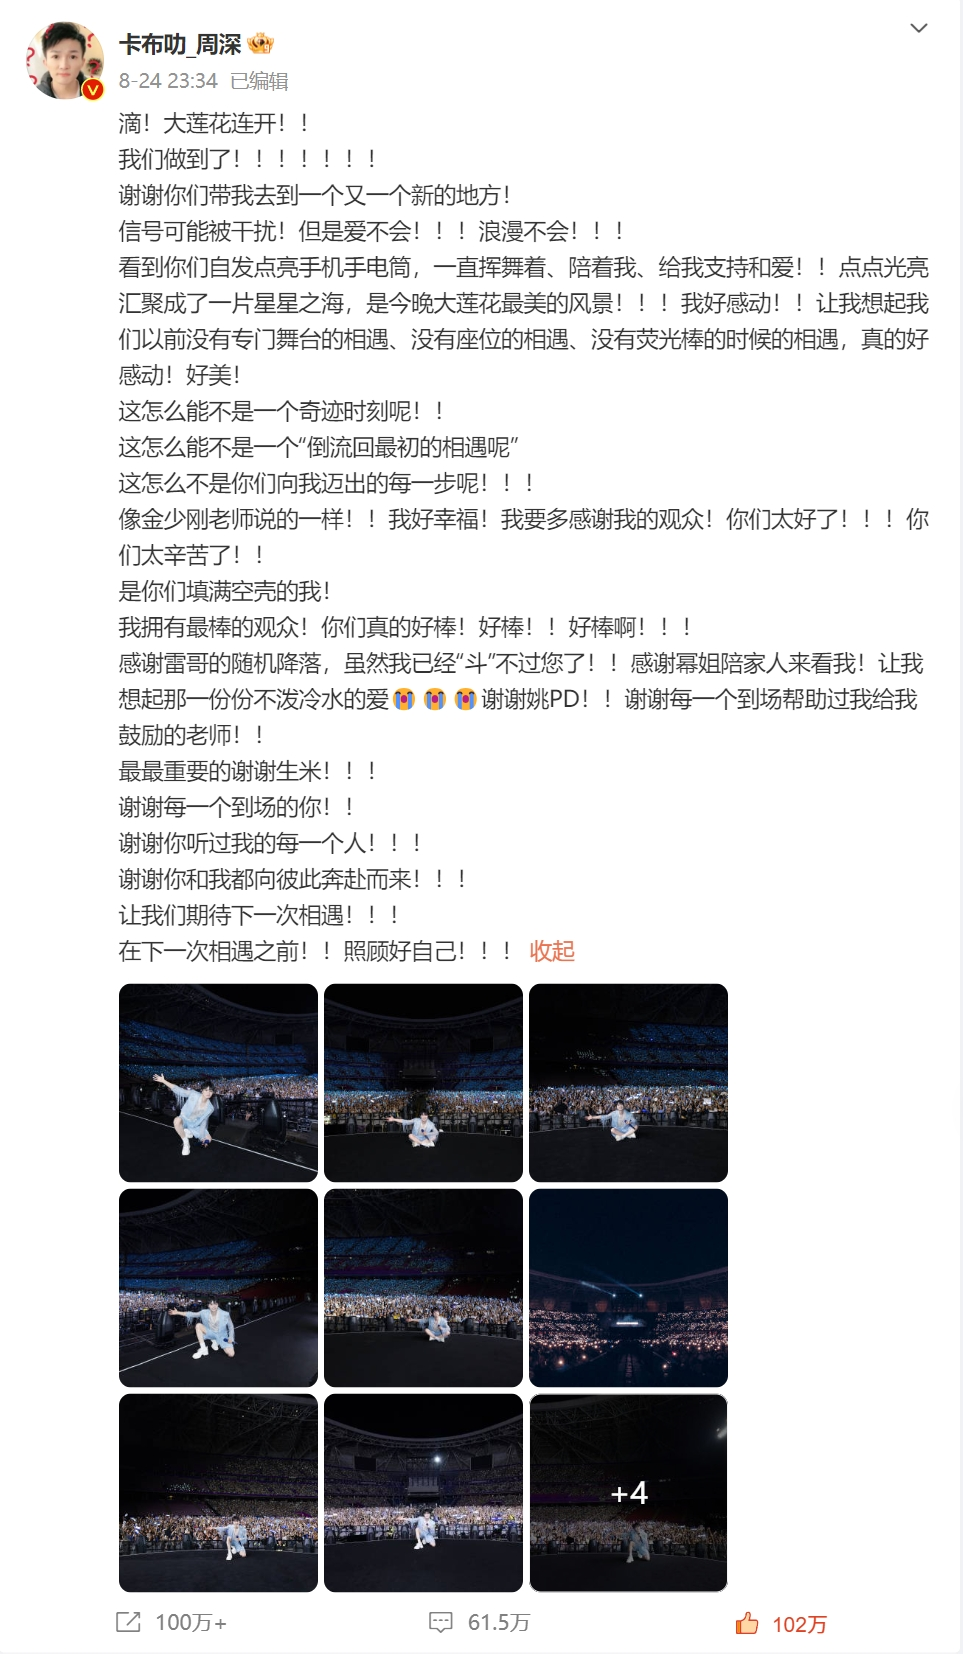
\includegraphics[width=400pt]{img/weibo/hangzhou-20240824} 

}

\caption{周深杭州奥体中心体育场演唱会结束微博 【@weibo-charlie】}\label{fig:unnamed-chunk-87}
\end{figure}

\chapter{2024.09.07沈阳场}\label{shenyang-20240907}

\begin{quote}
\textbf{\emph{你肯定没法想象你有多美好,因为遇见你,这人间更值得留恋啦!------ 周深}}
\end{quote}

\begin{figure}

{\centering 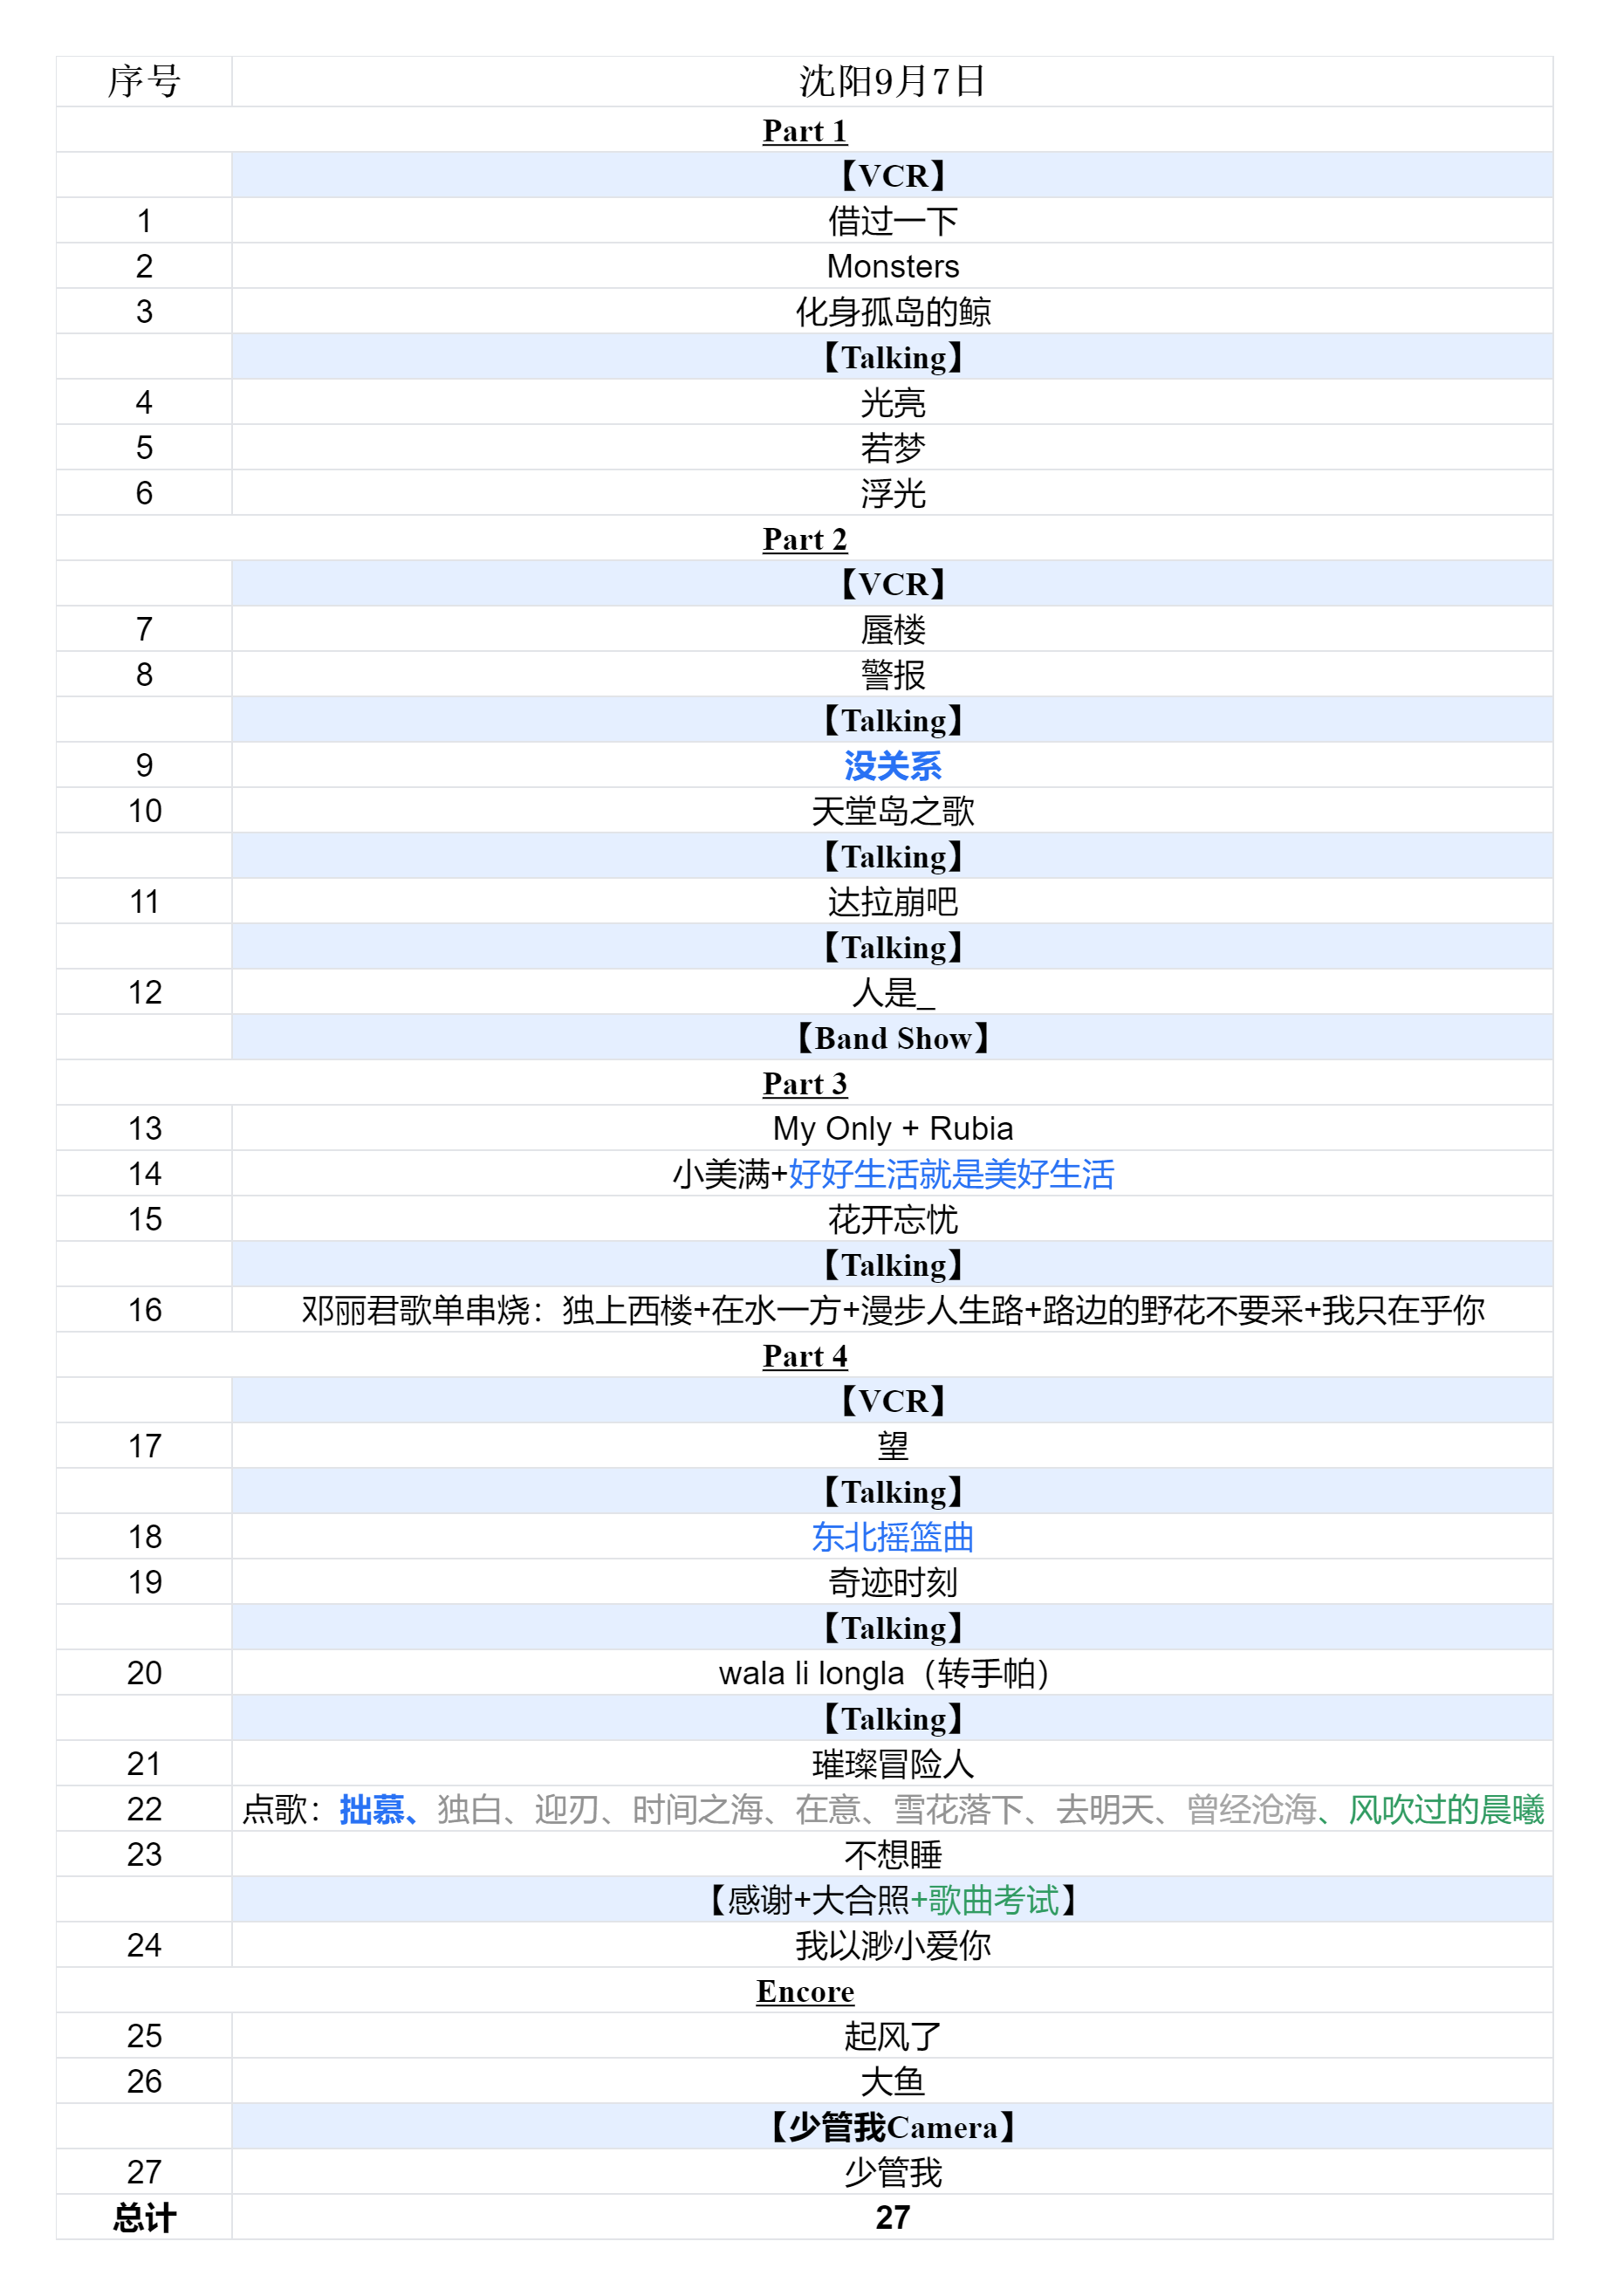
\includegraphics[width=320pt]{img/playlists/playlists-shenyang-20240907} 

}

\caption{2024周深9.29Hz巡回演唱会2024.09.07沈阳场歌单}\label{fig:unnamed-chunk-90}
\end{figure}

\newpage

\section{Part1}\label{shenyang-20240907-part1}

\hyperref[opening-vcr]{🎥【\textbf{开场VCR}】}

\hyperref[I-will-go-my-way]{🎵【\textbf{借过一下}】}沈阳的老铁们,你们好吗\textasciitilde{}

\hyperref[Monsters]{🎵【\textbf{Monsters}】} \textbf{\textcolor{red}{我爱你们~} }

\hyperref[hua-shen-gu-dao-de-jing]{🎵【\textbf{化身孤岛的鲸}】}老铁们你们好吗?跟我一起唱这首歌好不好?(米:好)\textasciitilde 到你们哦\textasciitilde 看台的朋友大声点儿\textasciitilde 到你们哦\textasciitilde(米:没有墙头)你们猜我信吗\textasciitilde(深:无论你有多少个墙头,也永远是我的国王和王后)

  沈阳的朋友们大家好,我是歌手周深,你们好吗?看台的朋友你们听到我的声音吗?你们在吗?吓我一跳,你们在吗?虽然我是出生于湖南,在贵州贵阳长大,但是东北我真的是太熟悉,就什么,呃,我说东北话,一点都不吭哧瘪肚啊,做事情尽量不磨磨叽叽,尽量麻溜的呀,然后,还有什么你瞅啥?瞅你咋地?哈哈哈,感觉这些都是不分任何地方,都非常熟悉的东北话。然后,一开始告诉我,要来沈阳开演唱会的时候,非常非常的激动,也非常担心,我在想就是,东北这样比较豪放的性格,大家比较喜欢快歌多一点,大家会不会听过一个歌手叫周深啊?(米:会)谢谢谢谢,谢谢你们\textasciitilde{}

  演唱会叫做9.29Hz,是因为我觉得我是一个比较渺小、比较特殊、或者说是比较不容易被听到的一个这样的存在,但是谢谢你们,能够在那么多声音当中,那么多人当中听到了我,\textbf{谢谢你们,让我在自己寻找自己的路上,没有那么的黑暗,我觉得非常非常的光亮,因为你们就是我的光亮,谢谢!}

\hyperref[silver-linings]{🎵【\textbf{光亮}】}你们也要记得光亮自己好吗?(米:好\textasciitilde)谢谢每一个发光的你,谢谢你照亮我,也要记得(深:光亮你自己)谢谢你们\textasciitilde{}
等下这首歌跟我一起来大声的唱好吗?(米:好)

\hyperref[ruomeng]{🎵【\textbf{若梦}】}哎呀,大兄弟大妹子,干哈呢?宝你个头啊,会唱吗?(米:会)看台的朋友等下要大声点哦\textasciitilde 到你们喽,(米:往事流转在你眼眸)好听!看台的朋友\textasciitilde 谢谢你们\textasciitilde 到你们喽\textasciitilde 来,大声点\textasciitilde 谢谢你们,全场一起\textasciitilde(深:惟愿你你你\ldots 你你你你能得到拯救,因为你们,我才得到拯救)我知道,我要比,就是很多歌手会多一道要被接纳的过程,谢谢你们愿意看见我,你们看见了我,所以我觉得我们都是很棒的人,谢谢你们听到了我!在这人世间恍惚三万天当中,好庆幸能有某一天或者一首歌的时间遇到你!

\hyperref[floating-light]{🎵【\textbf{浮光}】}(烟花🎆)\textbf{你肯定没法想象你有多美好,因为遇见你,这人间更值得留恋啦!}

\section{Part2}\label{shenyang-20240907-part2}

\hyperref[senself-vcr]{🎥【\textbf{反深代词VCR}】}

\hyperref[mirage]{🎵【\textbf{蜃楼}】}(红框墨镜)

\hyperref[the-giver]{🎵【\textbf{警报}】}谢谢\textasciitilde{}

  大家好,我是歌手周深,你们好吗?哇,没想到,来沈阳开演唱会太幸福了,因为你们太热烈啦,谢谢你们!都听说在演唱会,如果指哪里,哪里的声音就会很大声,是这样的吗?那这边呢,那如果我指看台的朋友,那边呢,那边呢,哇,好神奇啊,那如果是这样呢,谢谢你们\textasciitilde{}

  大家听到的第一部分的歌,是可能大家比较熟悉的我,比较飘渺比较古风。刚才演唱的歌曲,是我的新专辑反深代词的两首歌,希望大家能够去听一下这张新专辑。然后刚才演唱的蜃楼,说的是执念,每个人都有好的执念和坏的执念,也希望不要被他困住。然后第二首歌是警报,是送给每一个忘记爱自己的人,因为你们一直在照顾所有人但忘记照顾到自己,有这样的人吗?接受到这样的警报了吗?那接下来这首歌呢,也是我非常喜欢的一首歌,因为现在我们每个人压力都很大,就发现很多时候,因为很多采访就问我,\textbf{如果我有魔法的话,我最想要有个什么样的魔法,我说我想要拥有,可以把别人变成小孩子的魔法,因为小孩子就可以想哭就哭,想笑就笑,想吃就吃,}因为我们现在压力很大,就很多时候就觉得,哎呀,想哭会不会担心场合会不会合适,想笑你会觉得,哎呀,会不会有点尴尬,想吃又会有各种困扰,就很多时候,都应该给自己,就是被自己,自己把自己的空气都抽空之后,要给自己,要给自己说一句,没关系。希望你,因为这世界上是没有万能的答案的,但希望你在那么苛求自己的时候,也千万不要忘记给自己松那么一颗扭扣。告诉自己没有一百分也没有关系,你不完美也没关系,因为依然有人会爱你,听到了吗?看台的朋友们听到了吗 ?\textbf{\textcolor{red}{我爱你们~} }

\hyperref[life-is-like-a-box-of-chocolates]{🎵【\textbf{没关系}】}看台的朋友,你们在吗?(深:其实都没有关系)不对,\textbf{你们在,是件非常有关系的事情\textasciitilde{}}好好爱自己好吗?(米:好)

\hyperref[haven-song]{🎵【\textbf{天堂岛之歌}】}谢谢大家,谢谢大家愿意花时间来看我,然后也愿意,听到我新专辑的新歌,谢谢你们,沈阳的老铁们真的太给力啦,谢谢\textasciitilde{}

  那接下来我要给大家出一道考题,我有一个非常开心的舞台,但它好像是个,算是半个,四分之一个,五分之一个童话故事,你们知道是什么吗?(达拉崩吧)那你们记得里面角色的名字吗?(米:记得)哦,那我们考一考,它的主角叫达啦?(米:达拉崩吧斑得贝迪卜多比鲁翁)这么厉害,那他砍的那条恐龙名字叫做昆图?(米:昆图库塔卡提考特苏瓦西拉松)你们比我还熟悉这首歌那你们来唱好了,哈哈哈,那等下跟我一起来唱唱这个童话故事好吗?(米:好\textasciitilde)看台的朋友们等下也要唱得很大声哦,好不好?(米:好\textasciitilde)谢谢你们\textasciitilde{}

\hyperref[dalabengba]{🎵【\textbf{达拉崩吧}】}一起\textasciitilde 看台的朋友\textasciitilde 现在到你们喽,准备好了吗?复习一下,是谁砍了谁,救了谁,又回到了哪里?于是\textasciitilde(米:达拉崩吧斑得贝迪卜多比鲁翁)砍向\textasciitilde(米:昆图库塔卡提考特苏瓦西拉松)然后\textasciitilde(米:昆图库塔卡提考特苏瓦西拉松)咬了\textasciitilde(米:达拉崩吧斑得贝迪卜多比鲁翁)最后\textasciitilde(米:达拉崩吧斑得贝迪卜多比鲁翁)再来一遍哦,他叫达啦?(米:达拉崩吧斑得贝迪卜多比鲁翁)看台的朋友在大声点,他叫?(达拉崩吧斑得贝迪卜多比鲁翁)这么爱念,(深:要念你来念吧\textasciitilde)沈阳真的是,太棒啦\textasciitilde{}

  嗨,很开心,大家能够通过很多歌舞台认识我,像达拉崩吧啊,像monsters,当然我也很开心可以用自己的声音去参与到电视剧、或者是电影当中,接下来我要唱的这首歌叫做人是,你们会唱吗?真的会还是假的会,因为它真的有点高,没关系是吧,来,试一下,全场试一下哦,看台的朋友,听好了吗,考人是哦,好了吗?(深:让思死亡觊觎我)(米:)背不了词了吧?那等下希望你能跟我一起唱这首人是。\textbf{你们都是最棒的人\textasciitilde{}}

\hyperref[renshi]{🎵【\textbf{人是\_}】}谢谢大家\textasciitilde{}

\section{Part3}\label{shenyang-20240907-part3}

  Hello hello,大家好,你们知道我在哪吗,你们知道我躲哪吗?大家好,我是周深,好开心,真的从来没有想过自己有机会能够来沈阳开演唱会,我觉得很多事情发生,在自己脑海当中跟做梦一样,谢谢你们让很多,感觉遥不可及的事情都实现了,谢谢你们!看台的朋友,你们好吗?接下来要演唱的两首歌,是非常温暖,非常浪漫。这两首反正我觉得每次听完都是非常美好的歌,希望你们能够喜欢好吗?(米:好)就像这颗生命树一样,因为遇到你们,我才有更多的养分去寻找更好的自己,也希望我的歌声能够陪伴你们去寻找更好的自己好吗?(米:好)我们一起加油!(米:加油)

\hyperref[my-only]{🎵【\textbf{My Only}】}
\hyperref[rubia]{🎵【\textbf{Rubia}】}呃呃呃,刚有几个音都弹错了。又错了\textasciitilde 大家给我加油!人生就像这歌词(嘴瓢歌chi)人生就像这歌词写的一样,我们的人生,好像就像绽放如花朵一样,所以我们要珍惜我们每一次绽放的机会,好吗?

  在沈阳我好紧张啊,非常感谢你们愿意来,那接下来这首歌跟我一起好好唱好吗?这首歌你们唱的是我听过最好听的版本,交给你们喽\textasciitilde{}

\hyperref[happy-ending]{🎵【\textbf{小美满}】}(深:没什么大愿望)唱\textasciitilde 看台的\textasciitilde 跟我一起\textasciitilde 再大声点\textasciitilde 你们唱得太好啦\textasciitilde 看台的朋友也要大声唱哦\textasciitilde 大声点\textasciitilde{}\textbf{\textcolor{red}{我爱你们啊~}}全场\textasciitilde 谢谢我们沈阳的朋友们\textasciitilde 因为遇到你们啊,我每次听这首歌的时候,我就觉得所有的愿望都会实现,那不如我们就在这首歌当中许愿吧,好不好?我先给大家打个样,默默想想心中的愿望,321,就会看到你的愿望被挂在那棵许愿树上。现在全场跟我一起闭上眼睛,无论你多大,无论你是从事什么样职业的,此时此刻闭上眼睛,我们默默想个愿望,我们就在9.29Hz沈阳站,我们一起去种下这棵愿望树,想好你的愿望,但是愿望有一个要求,只能够许关于自己的愿望。你有多久没有问过自己啦?你有多久没有小小的放过一下自己呢?现在全场321,睁开眼睛,你们的愿望都会实现的,我们听到啦\textasciitilde(深:你们就是周深最好的陪伴)

\hyperref[live-happy-life-happy]{🎵【\textbf{好好生活就是美好生活}】}也要记得(深:人生多么美妙。。。新的一天我们一定)(米:好好\textasciitilde)谢谢你们,我们一定好好的\textasciitilde{}\textbf{最热烈的掌声给最棒的自己!}

\hyperref[no-worries]{🎵【\textbf{花开忘忧}】}说什么?(米:你好啊\textasciitilde)你好啊\textasciitilde 沈阳的朋友,我来你们家看你啦\textasciitilde 这首歌愿意跟我一起唱吗?(米:愿意)我们的思念,他们一定听得到对不对?(米:对)想他就表达出来吧,花开忘忧,愿你无忧,花开忘忧,(米:愿你无忧)

  谢谢你们,很开心,真的非常非常开心遇到了你们,(换衣服,米尖叫)但是我在换衣服时候有这么大的尖叫声,可能有点不开心,怎么比我唱歌的声音还大声。所以我刚才在唱好好生活就是美好生活,中间有一句,就是,好好陪你长大,好好陪你变老,我一看下面有非常小的小朋友,我就突然就心一酸,哎呀,我还能唱到多少岁呢?(米:一直唱下去)一直唱下去?我也没那么厉害。但是\textbf{我就觉得自己很幸福可以作为一个歌手,可以有很多歌曲一直在那里,只要你们想我的时候就可以打开那个文档},好吗?(米:好)所以我也觉得自己希望可以成为像邓丽君女士这样的歌手,无论是隔了多久,或者是在任何地方。他的每首歌当中几乎都存着每一个、很多人的时光胶囊,有他们很多的往事,所以我会继续努力,歌手周深一定要加油!但是因为每一个看到了我,听到了我,给我光的你们,歌手周深才能够一步一步从路边,再到live house,再到剧场,再到体育馆,再到我们沈阳体育场。谢谢你们,我一定会加油的\textasciitilde{}

🎵【\textbf{邓丽君组曲}】
\hyperref[one-in-the-building]{🎵【\textbf{独上西楼}】}跟我一起唱好吗?
\hyperref[on-the-water-side]{🎵【\textbf{在水一方}】}看台的朋友也要大声哦\textasciitilde 到你们\textasciitilde{}
\hyperref[walk-the-road-of-life]{🎵【\textbf{漫步人生路}】}摇起来\textasciitilde 沈阳的朋友,你们好吗?
\hyperref[only-with-me]{🎵【\textbf{路边的野花不要采}】}这首你们会唱吗?来喽\textasciitilde 到你们\textasciitilde(深:路边的野花,你不要采)记得不要采,千万不要采\textasciitilde{}
\hyperref[only-you]{🎵【\textbf{我只在乎你}】}你们会忘了我吗?(米:不会!)最好说话算数!\textasciitilde 看台的朋友\textasciitilde(深:除了你你你你你你\ldots\ldots 你,我不能感到一丝情意)谢谢你们\textasciitilde{}

\newpage

\section{Part4}\label{shenyang-20240907-part4}

\hyperref[thank-you-vcr]{🎥【\textbf{谢谢沈阳,谢谢你VCR}】}

\begin{figure}

{\centering 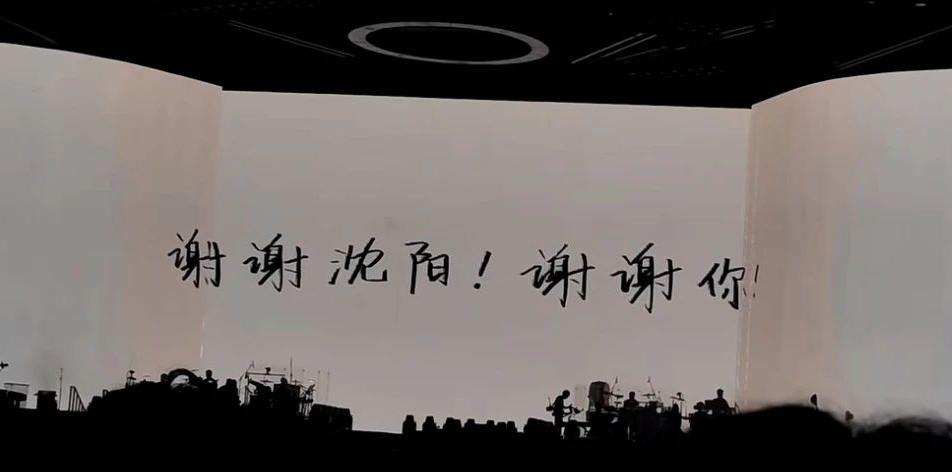
\includegraphics[width=400pt]{img/shenyang20240907/thank-shenyang} 

}

\caption{谢谢沈阳!谢谢你!}\label{fig:unnamed-chunk-91}
\end{figure}

\hyperref[hope]{🎵【\textbf{望}】}谢谢你们一直牵着那一根思念我的线\textasciitilde 谢谢你们,无论我去到哪里,都让我觉得像回家一样,谢谢你们\textasciitilde 跟我一起\textasciitilde 看台的朋友\textasciitilde(深:因为你们,我才心有所住,也希望你们,无论在哪,都不会孤独\textasciitilde)谢谢你们\textasciitilde{}

  其实每次在想到一个城市要唱什么歌的时候,我觉得最苦恼的就是到沈阳,因为关于东北的歌太多了,(俺们那嘎达都是东北人),还有(我的家在东北)对,太多太多了,(我的老家,就住在这个屯),哈哈哈,但后面我就发现,我听到一首歌叫做东北摇篮曲,我就觉得它非常非常的美好,就是无论我们在任何地方,你就会觉得突然就有一个非常温暖的拥抱,去抱住你,可能在你需要温暖的时刻,或者觉得你在孤单的时候,所以我就觉得我要唱这首歌,我觉得希望无论在任何地方,只要你需要我的时候,我都在这,好吗?(米:好)因为我听说每一个东北人,好像他的长辈都用这首歌,几乎都是用这首歌哄他睡过觉,对不对?如果你没有的话,那今天听听看,因为我从小我妈妈没有给我唱过摇篮曲,因为她唱歌跑调,哈哈哈,可能唱完之后我就一直在笑,就睡不着,但总之希望你们能够喜欢这首东北摇篮曲\textasciitilde{}

\hyperref[lullaby]{🎵【\textbf{东北摇篮曲}】}无论你在哪,都要记得,谁还不是个宝宝呢,答应我,照顾好自己好吗\textasciitilde 一定要照顾好你这个宝宝哦\textasciitilde{}

  我发现我生命当中有太多我从来没有想过,但是最后实现了的事情,比如当歌手,比如被你听见,比如我看观众朋友的时候,好像有五六岁的小朋友,对不对?还有很多甚至是60岁、70岁以上的人,我觉得这些在我生命当中他都是奇迹时刻。所以啊,不要太着急,很多事情甚至是很多好事都是在你意料之外的,你要相信自己,好吗?(米:好)我们不是一定要挪动一座山才叫做奇迹,我们只要一直在寻找自己最好的那个自己的路上,我们就是一道风景,好不好?享受属于我们的奇迹时刻\textasciitilde{}

\hyperref[magic-moment]{🎵【\textbf{奇迹时刻}】}嗨起来\textasciitilde 看台的朋友,你们好吗?【魔术时间】这是一根小小的棍子,哈哈,放不进去。没关系,我还有。在我手忙脚乱的时候,给我一点掌声好吗?这样奇迹才能够诞生,芜湖\textasciitilde 哈哈哈哈哈哈哈,我变的魔术精彩吗?(米:精彩)

\begin{figure}

{\centering 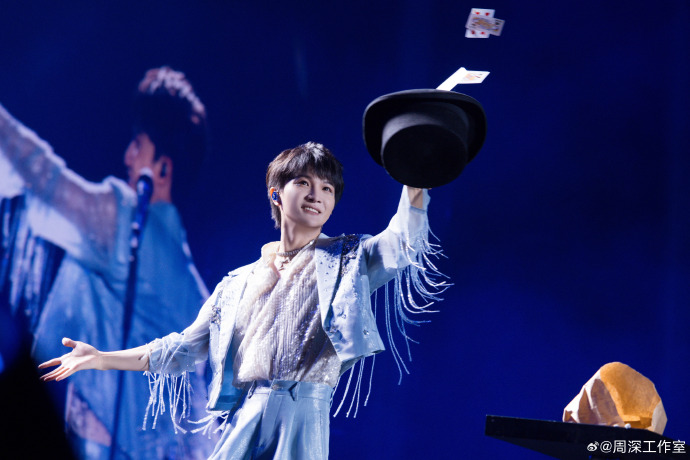
\includegraphics[width=400pt]{img/shenyang20240907/001} 

}

\caption{萌术师!【@weibo-charlie-studio】}\label{fig:unnamed-chunk-92}
\end{figure}

  谢谢你们愿意接受每一刻我的碎片,哪怕是不完美的有一些些残缺的碎片,谢谢你们!也告诉你们想学任何一个新的技能,多少岁开始都不会迟好吗?(米:好)看台的朋友们听到了吗?在反深代词专辑当中有一个快乐密码,大家知道吗?叫做wala li longla,我们全场试一下好不好?wala li,wala li long,wala li longla。那等一下跟我一起大喊这个快乐密码好不好?这样你生活当中所有的烦恼都会消失的。Magic\textasciitilde{}

\hyperref[wala-li-longla]{🎵【\textbf{wala li longla}】}到你们\textasciitilde 看台的朋友们\textasciitilde 全场的朋友跟我一起念这个快乐密码好不好?(米:好)我念什么你们就念什么哦(猫猫扭秧歌,转手绢)嗨起来,wala,wala li,wala li long,wala li longla,wala,看台的\textasciitilde wala li,wala li long,wala li longla,(唢呐\textasciitilde)你们是最棒的!\textasciitilde 全场最后一遍\textasciitilde 谢谢你们\textasciitilde 还想听一次,321\textasciitilde(米:wala li longla)

  我们沈阳的3.6万多的观众朋友们,你们是最棒的!谢谢你们,大家刚才听那个摇篮曲觉得好听吗?(米:好听)有没有快听睡着的?(米:没有)这个问题很难回答,堪称是高情商里面一定要考的一道题。你们觉得我唱的摇篮曲好听对不对?(对)那如果你们没有听睡着,那是失败还是成功呢?(米:成功)凭什么?那请问摇篮曲的目的是?是不睡觉啊?好了,谢谢你们,我经常,我特别最大的感触就是每次看到你们都好像是第一次看到你们一样的激动。我都特别的紧张,你们感受的到吗?因为我看见每一个,应该说是盛装出席,或者是每一个认真对待这一次聚会的人,我都觉得好幸福,大家都以自己最舒服的状态来见面\textasciitilde{}
您好,虽然很冷漠,但是努力地挥了手,看台的朋友们你们好吗?(米:好)四个字,何德何能?谢谢你们能够让一个非常普通的小男孩去追逐他的梦想。还是那句话,周深可以的,你也可以,相信我,加油好吗,每一个璀璨冒险人\textasciitilde{}

\hyperref[adventurers]{🎵【\textbf{璀璨冒险人}】}一起\textasciitilde 再来\textasciitilde 你们都是自己的英雄\textasciitilde(米唱:还想要继续吗?)要\textasciitilde 大声点\textasciitilde 璀璨冒险人们,向前冲吧\textasciitilde 谢谢你们\textasciitilde{}

【\textbf{点歌环节}】现在到了我们的,点(歌)\textasciitilde 干哈呢,这是干哈呢?宝你个头啊,宝你个头乘以3.6w啊。(米:宝贝\textasciitilde)怎么会各个年龄段都在喊,怎么回事\textasciitilde 到了我们的点歌环节了,这也是沈阳站最害怕的环节,你知道为什么吗?因为我害怕我唠不过东北的朋友啊,我害怕我被欺负\textasciitilde 好,到了我们的点歌环节,我们全场倒数5个数字,一起选中那个点歌的朋友,好不好?这几首歌都是相对来说没有那么热门的歌,但是我相信他一定是某个朋友心中的那个宝藏歌单,对不对?所以谢谢你们。那么今天是由谁点出我们沈阳站的点歌歌曲呢?全场倒数5个数字,大家大声点,54321,呦,你好,嗨,小朋友,但是不是你哟,对不起,你在哪里?哪里?在,他在,哎,你好,(米:你好)跟我们沈阳的朋友打个招呼。(米:沈阳的朋友们,大家好)通过这个打招呼感觉得我唠不过她,怎么说?哈哈哈,这位朋友怎么称呼您?(米:你可以叫我尾巴)尾巴?那也可以叫你乙巴,是不是?(米:也可以)也可以,你是来自哪里的朋友啊?(米:我是山东的朋友啊)山东朋友,我们欢迎山东的朋友。(米:谢谢大家)那你主持吧,哈哈,你今年,可以方便说多大吗?(米:我22)那,还好啦,也就是我八九年前,(米:宝贝\textasciitilde)喂,我只能说,呜呜呜呜呜(深拿着扑克牌5)哈哈哈,你快走吧(深拿着扑克牌8),哈哈哈,也祝你发发发发发发发。那你应该还在刚毕业是吗?(米:刚毕业,刚入职)那我们预祝他工作顺利。听我唱歌听多久了?(米:快五年了)听五年了?你听我的第一首歌是?(米:第一首歌是不再流浪)哦,我正要说除了大鱼,谢谢,那你看到我的印象很深的第一个舞台是(第一个舞台应该是达啦崩吧)哦,那请问里面的那个公主的名字叫?答不出来,我们今天的课就先上到这里了。(我答得出来,公主米娅莫拉苏娜丹妮谢莉红)太厉害了,真厉害,真棒,好羡慕哦。来看一下吧,这9首歌当中有没有你想听的歌?(米:我想听第九首歌拙慕)其他朋友也想听这首是吗?为什么是这首啊?(米:因为这首是我入坑之后开始考古印象最深的一首)好专业的两个词,入坑和考古,朋友们,入坑是什么意思?就是喜欢听周深唱歌。考古是什么意思啊?应该听得明白吧,叔叔还是哥哥啊?你没有在看我,哈哈哈。好,那我们就唱出这首拙慕,希望你能够喜欢。谢谢尾巴。\textbf{宝你个头宝你个头宝你个头宝你个头宝你个头宝你个头宝你个头\ldots\ldots 坐下,宝你个头宝你个头宝你个头宝你个头宝你个头\textasciitilde{}}好,开玩笑啦,尾巴还有什么话要说,她还有一句话老师,话筒给她一下,她还有一句话,宝你个头看台朋友们\textasciitilde(米:\textbf{你一直唱,我们一直听,周深值得,生米爱你!})谢谢谢谢,谢谢生米们,谢谢,也谢谢每一个听过我的人,因为我真的认为我比很多歌手会多一道,比较容易,怎么说,被接纳的那段过程,所以我觉得愿意支持我来看我的,都是最美好的人,谢谢你们,最美好的朋友们,看台的朋友们,你们听到了吗,谢谢你们\textasciitilde 这首拙慕\textasciitilde{}

\hyperref[inferior-admiration]{🎵【\textbf{拙慕}】}(深深戏精上线,然后以为自己进错拍了)进错了,重来,我是不是应该没有进错?对不起,我好好唱歌!拙慕!

  谢谢你们愿意花时间听我唱歌,谢谢你们来,谢谢你们还在\textasciitilde{}

\hyperref[keep-playing]{🎵【\textbf{不想睡}】}跟我一起\textasciitilde 谢谢你们\textasciitilde 谢谢在这个宇宙当中我们相遇啦\textasciitilde 全场一起\textasciitilde 大声点\textasciitilde 看台的朋友\textasciitilde{}

  大家今天来这里还开心吗?(开心)我们演唱会快到尾声哦。但是每一次演唱会结束,它不代表就是结束,因为在这个宇宙当中,我是说真的,就是我们荧光棒发出的光子,或者说我们手电筒那个发出的光子,会在宇宙当中持续很多很多年之后,我们就哇我们又相遇。\textbf{也希望今天这段美好的回忆能够在你需要的时候给你一个好好的、暖暖的拥抱,}好吗?(米:好)因为这段温暖的回忆一定可以让我不害怕做任何事情会失败或者说会不完美,因为我都相信此刻的温暖它会永恒的存在,对不对?所以要感谢我们,非常非常多让我们好好见面的朋友们,好不好?(米:好)

  谢谢大家帮我们,感谢场地支持,沈阳奥林匹克体育中心体育场。感谢本次巡演的全程主办,北京时代立方文化传播有限公司。这里面有个小插曲,告诉大家一下。因为我们杭州场第二站的时候,我们的荧光棒信号稍微有一点点干扰,我们的主办,我们的全程主办,他也全程在担心会不会到感谢我的时候,大家喊的是倒闭,我就觉得今天看到我们的老师们,大家都是,老师,加油啊,大家是有什么不开心吗?仔细一问,嗯\textasciitilde 感谢我们的全程主办时代立方。谢谢你们,\textbf{也谢谢我们最可爱最棒的观众},我们也许,不叫也许,我们一定有很多很多不完美的地方,包括我一定也有很多没有办法唱到完美的歌,但是这个就是真实,这个就是最完美的爱,对不对?(米:对)我们不好的地方还会加油的,谢谢你们来。谢谢我们的演唱会制作单位毕应。小朋友你好可爱啊,谢谢我们的总导演周佑洋,庄惟惞。感谢我们的音响总监金少刚,那大家一定要相信有很多像金老师这样在就是默默的一直在支持你,在我需要帮助的时候就会出来的,那样的人一直在爱着你,所以要好好照顾,这样要好好照顾自己,这样爱你的人才不会担心。听到了没有?(好)太小声了。听到了没有?(听到啦)感谢我们的音乐总监龙隆老师,感谢我们的乐队老师们,感谢我们的合唱老师们,垂爱大家,东北话是这么说吧?感谢我们的舞蹈团队SDT ShowPro。谢谢服装团队设计师劳伦斯·许工作室,时装品牌Windowsen,感谢我们无论是刮风下雨都可以把我们的舞台搭得漂漂亮亮的,然后也可以让大家就是尽量照顾到大家的音响工程,南京奥斯泰。感谢让大家听到好听的声音的,至少让我的声音尽量好听一点的调音团队,乐尔工作室,但是他们也会及时让我听到你们的声音,因为你们唱的太好听了哇。感谢音频工程北京立超舞台集团也是我们一起搭建舞台的,也感谢周深工作室的小伙伴们。(米:哇)还是一样,我们会继续努力的,我们会加油的。再一次谢谢我们的工作室的小伙伴们。感谢微博(倒闭),感谢微博音乐(倒闭),感谢微博演出(倒闭),你们这是感谢吗?哈哈哈,当然要感谢,最快乐最轻松,又特别好吃又非常非常多惊喜又非常非常多可爱的人的沈阳。呦吼,非常感谢沈阳这座城市,真的是每来一次都会更加爱他几分,也感谢我们的沈阳公安安保团队,感谢文化、消防等所有职能部门的大力支持,保障我们这场演出的顺利进行。还要感谢所有台前幕后的工作人员们,特别是我们的志愿者们啦,辛苦啦,当然最重要的是什么?要感谢的是来到现场的每一个你,还有在看台的你哦,谢谢你们,没有你们这一切都是不可能发生的,所以我们来大合照吧。

  好,我们先是中间的朋友,大家辛苦喽,千万不要生病了,照顾好自己哦。321,好,我们这边的朋友。321,你看我脑袋每次都会,这边不挡。1321,我每次要合唱时候,我递一下麦,嗨,往事流转,(米:在你眼眸)哇,你们唱的太好听了,来,321,惟愿你能得到拯救,哦,那下次(你的眼光)。哇塞,你们唱得太好了吧,这边的朋友来,我们这边的朋友坐好,注意安全,安全第一,321,嗯,那这首会唱吗?我们苍老的时候\textasciitilde(米:就回到小时候。。。),你们怎么背的清了这么多词?你们什么时候考虑开演唱会啊?来这边的朋友,321。还有这边的哟,大家辛苦了,321。

  刚才演唱的不想睡是卡布的晚安曲,那周深也有一首我尽量不哭的一首晚安曲,叫做我以渺小爱你。在这个宇宙当中,已经不要说是在这个宇宙当中,在人群当中,尤其是北方像沈阳站的人群当中,我渺小到几乎可能我自己都找不到,我一直都知道自己是一个非常渺小的存在,而且我也相信有很多人跟我有一样的感受,但是要相信自己,你的力量真的很强大,你们让一个普普通通这么渺小的男孩越来越靠近他的梦想,让他有那么多束光,可千万别忘那些光都是来自你身上的。好吗?(米:好)谢谢你们,我以渺小爱你\textasciitilde{}

\hyperref[loving-you-in-my-humble-way]{🎵【\textbf{我以渺小爱你}】}你们知道吗,这一切太美了,美好得都让我觉得不相信它好像真的发生过,无论我还能唱多少首歌,或者是能不能唱高音,或者任何一首歌,但是谢谢你们能够给我一个副歌的可能,一首歌的可能,谢谢你们给我这么不朽的支持\textasciitilde(我以渺小爱你同行的旅程)谢谢每一个愿意听我唱歌,无论你是不是生米,你听到我就是给我最大的善意和支持。(我以短暂爱你不朽的旅程)谢谢你们,\textbf{\textcolor{red}{我爱你们} },沈阳的朋友们\textasciitilde{}

\section{Part5}\label{shenyang-20240907-part5}

\hyperref[the-wind-rises]{🎵【\textbf{起风了}】}谢谢你们还在\textasciitilde 谢谢你们\textasciitilde 以爱之名,(深:你还愿意吗?)(米:愿意)

\hyperref[big-fish]{🎵【\textbf{大鱼}】}谢谢你们\textasciitilde{}

  最后还想再耽误一下大家一点时间,再听一首专辑里的歌好不好?(米:好)专辑这首歌它叫做少管我,如果用东北话说的是,那咋了?是这样说吗?还是爱咋咋地?都不是啊。少管我应该咋说?喊我滚,不太礼貌吧,什么管我,就是少管我,对吧?等一下我们就大概是全场倒数5个数字,然后我们摄像机抓到了谁,就要做我们少管我的标志性动作好不好?就是,嘿,少管我好不好,但是注意不要打到前面朋友的脑袋,少管我这首歌他是说让我们不要,就是为自己,就是怎么说,我想想,用最短的话来总结,少管我就是要让我们为自己负责,在寻找我们最好的那个自己的路上遇到很多问题,我们不要用争吵,不要用所有的那些不好的情绪去面对,我们可能就轻声说一句,嘿,少管我,因为做自己这件事情,没有人比你们做得更好,所以千万不要误解的少管我,让我们全场倒数五个数字,52321,停\textasciitilde oh,就是你吧?应该是拿这个,就是你,诶那个六方形的脑袋,哈哈哈,你们是怎么接纳这个形象的呀?你在哪里?你好,怎么称呼你?朱朱?(手机显示宝贝)宝你个头,你是来自哪里的?等一下,后面那个六边形的,它的辫子去哪啦?看来发量很多,我很放心,哈哈。朱朱你是来自哪里的朋友?先把手机给我关掉。上海的,沈阳的朋友欢迎一下我们来自上海的朋友好不好?沈阳好不好玩?你吃个鸡架,鸡架可好吃了。你要吃他们的那个麻辣烫,就我吃了很多,发现沈阳的麻辣烫不一样,而且他们的鸡架有很多种做法哟,有烤的,有炸的、有拌的,有什么多?那你吃的是哪个口味的呢?吃的是拌的。那再试一下其他口味好吗?什么时候听我的歌哦?听了我的歌四年了。哦,那你准备好,你准备好用最大的声音让全场听到,少管我了吗?准备好了,全场,大家听一下,如果没有的话就是喊到喊破喉咙,321。这边的朋友听到了吗?来,再来一遍。321谢谢朱朱,希望你天天开心。

  我们再来选一位,全场倒数五个数字,54321。哎呦,您是来自哪里的?沈阳本地?哎呀妈呀,你好啊。你多大呀?21?哦,弟弟你好啊。突然对他的尊重少了很多。弟弟听哥哥的歌听多久了哈?等一下,你21岁,也就是说我出道的时候你\textasciitilde 刚\textasciitilde 出\textasciitilde 生\textasciitilde,哦哦哦哦,你10岁了,对不起我这个数字算得,哈哈哈,我出道时候你10岁了。你什么时候听我歌的啊,以为自己出道20年了,不好意思,哈哈哈,听两年了。你听我的第一首歌是哪首歌?哦,大鱼,那你怎么,我居然在沈阳找到一位i人?你是i人还是e人?i的很明显,i人,你要用最大的声音喊出少管我,你愿意吗?你愿意哈,用最大的声音。如果前面的人没有捂耳朵都不算数,你直接开捂了有点假吧。来321,谢谢。怎么称呼您来着?叫你什么?小林?小林。好,谢谢小林。谢谢谢谢谢谢谢谢,原来东北还是有内向的朋友的,每次来到我们东北我都觉得我好内向。就是大家就是就给我一种非常熟悉非常温暖的感觉,但突然觉得我是说不过你们的,但是任何时候都,嘿少管我好吗?(米:好)希望你们都成为最好的自己\textasciitilde{}

\hyperref[watch-ur-manners]{🎵【\textbf{少管我}】}看台的朋友,摇起你们的荧光棒哦\textasciitilde 跟我一起\textasciitilde321\textasciitilde 要大声点哦\textasciitilde 全场跟我一起\textasciitilde54321\textasciitilde 你们是最棒的\textasciitilde 全场跟我,54321\textasciitilde 谢谢你们来,54321\textasciitilde 谢谢你们\textasciitilde 谢谢你们\textasciitilde 看台的朋友,谢谢你们\textasciitilde54321\textasciitilde 谢谢你们,\textbf{我爱沈阳\textasciitilde{}}54321\textasciitilde 谢谢大朋友小朋友们,一定要注意安全,手机不要掉了,证件不要掉了,看台的朋友们辛苦啦,谢谢你们听到我,谢谢你们来,谢谢你们还在\textasciitilde54321\textasciitilde 谢谢\textasciitilde54321\textasciitilde 谢谢你们\textasciitilde54321\textasciitilde 你们是最棒的\textasciitilde 注意安全,证件不要掉了,一定要平平安安的,大家答应我好吗?我们一定会再见的,在我们下次见面之前,照顾好自己,byebye\textasciitilde{}

\begin{center}\rule{0.5\linewidth}{0.5pt}\end{center}

\begin{figure}

{\centering 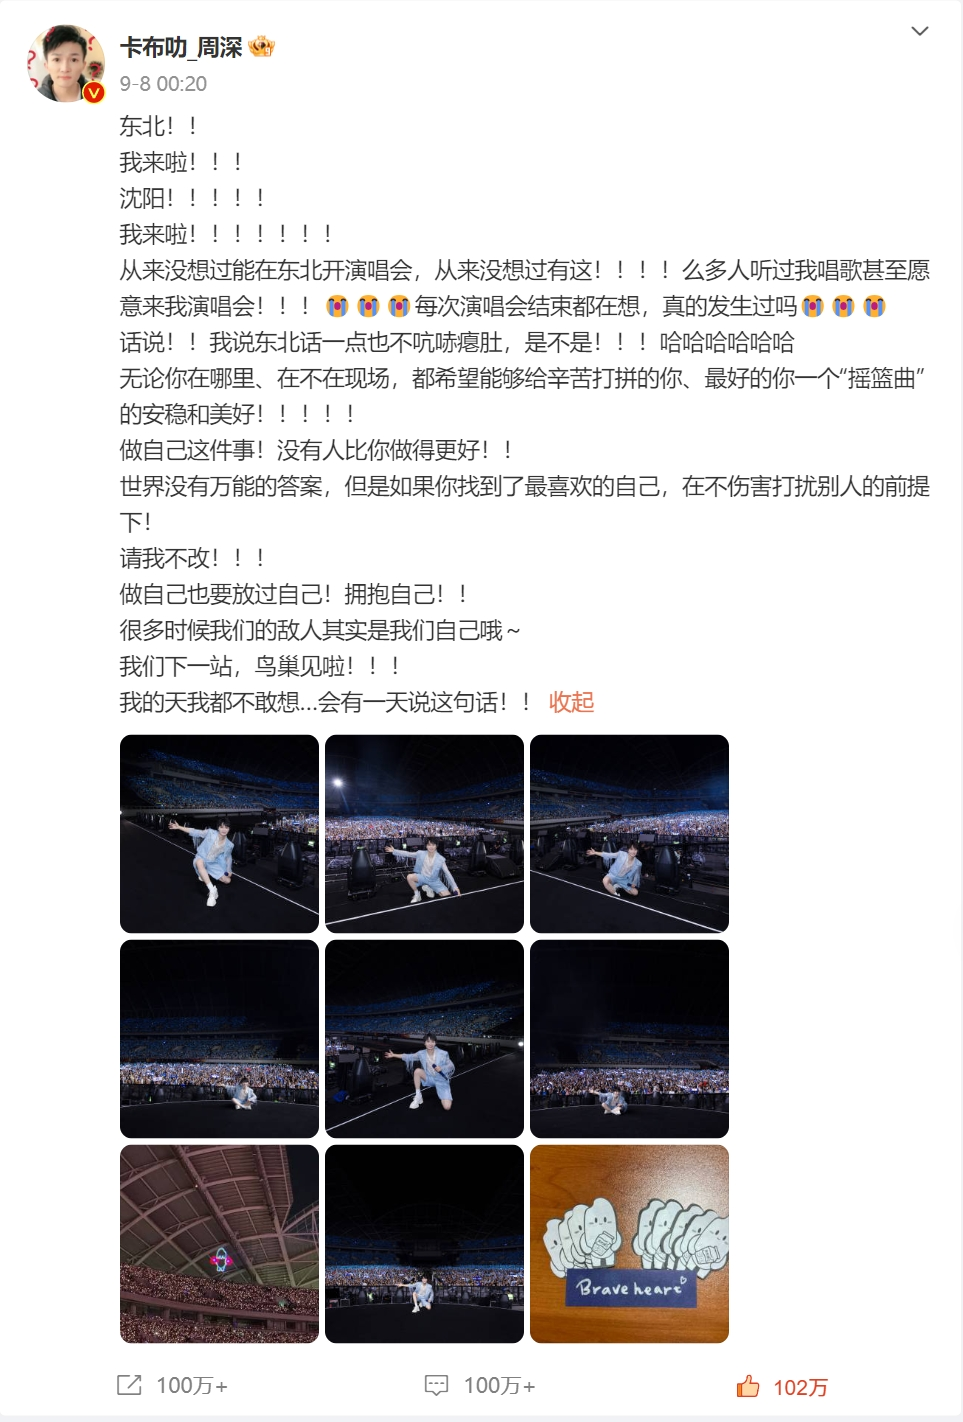
\includegraphics[width=400pt]{img/weibo/shenyang-20240908} 

}

\caption{周深沈阳奥林匹克体育中心体育场演唱会结束微博 【@weibo-charlie】}\label{fig:unnamed-chunk-93}
\end{figure}

\chapter{2024.09.21北京场}\label{beijing-20240921}

\begin{quote}
\textbf{\emph{你们是世界上最美好的存在哦。 ------ 周深}}
\end{quote}

\begin{figure}

{\centering 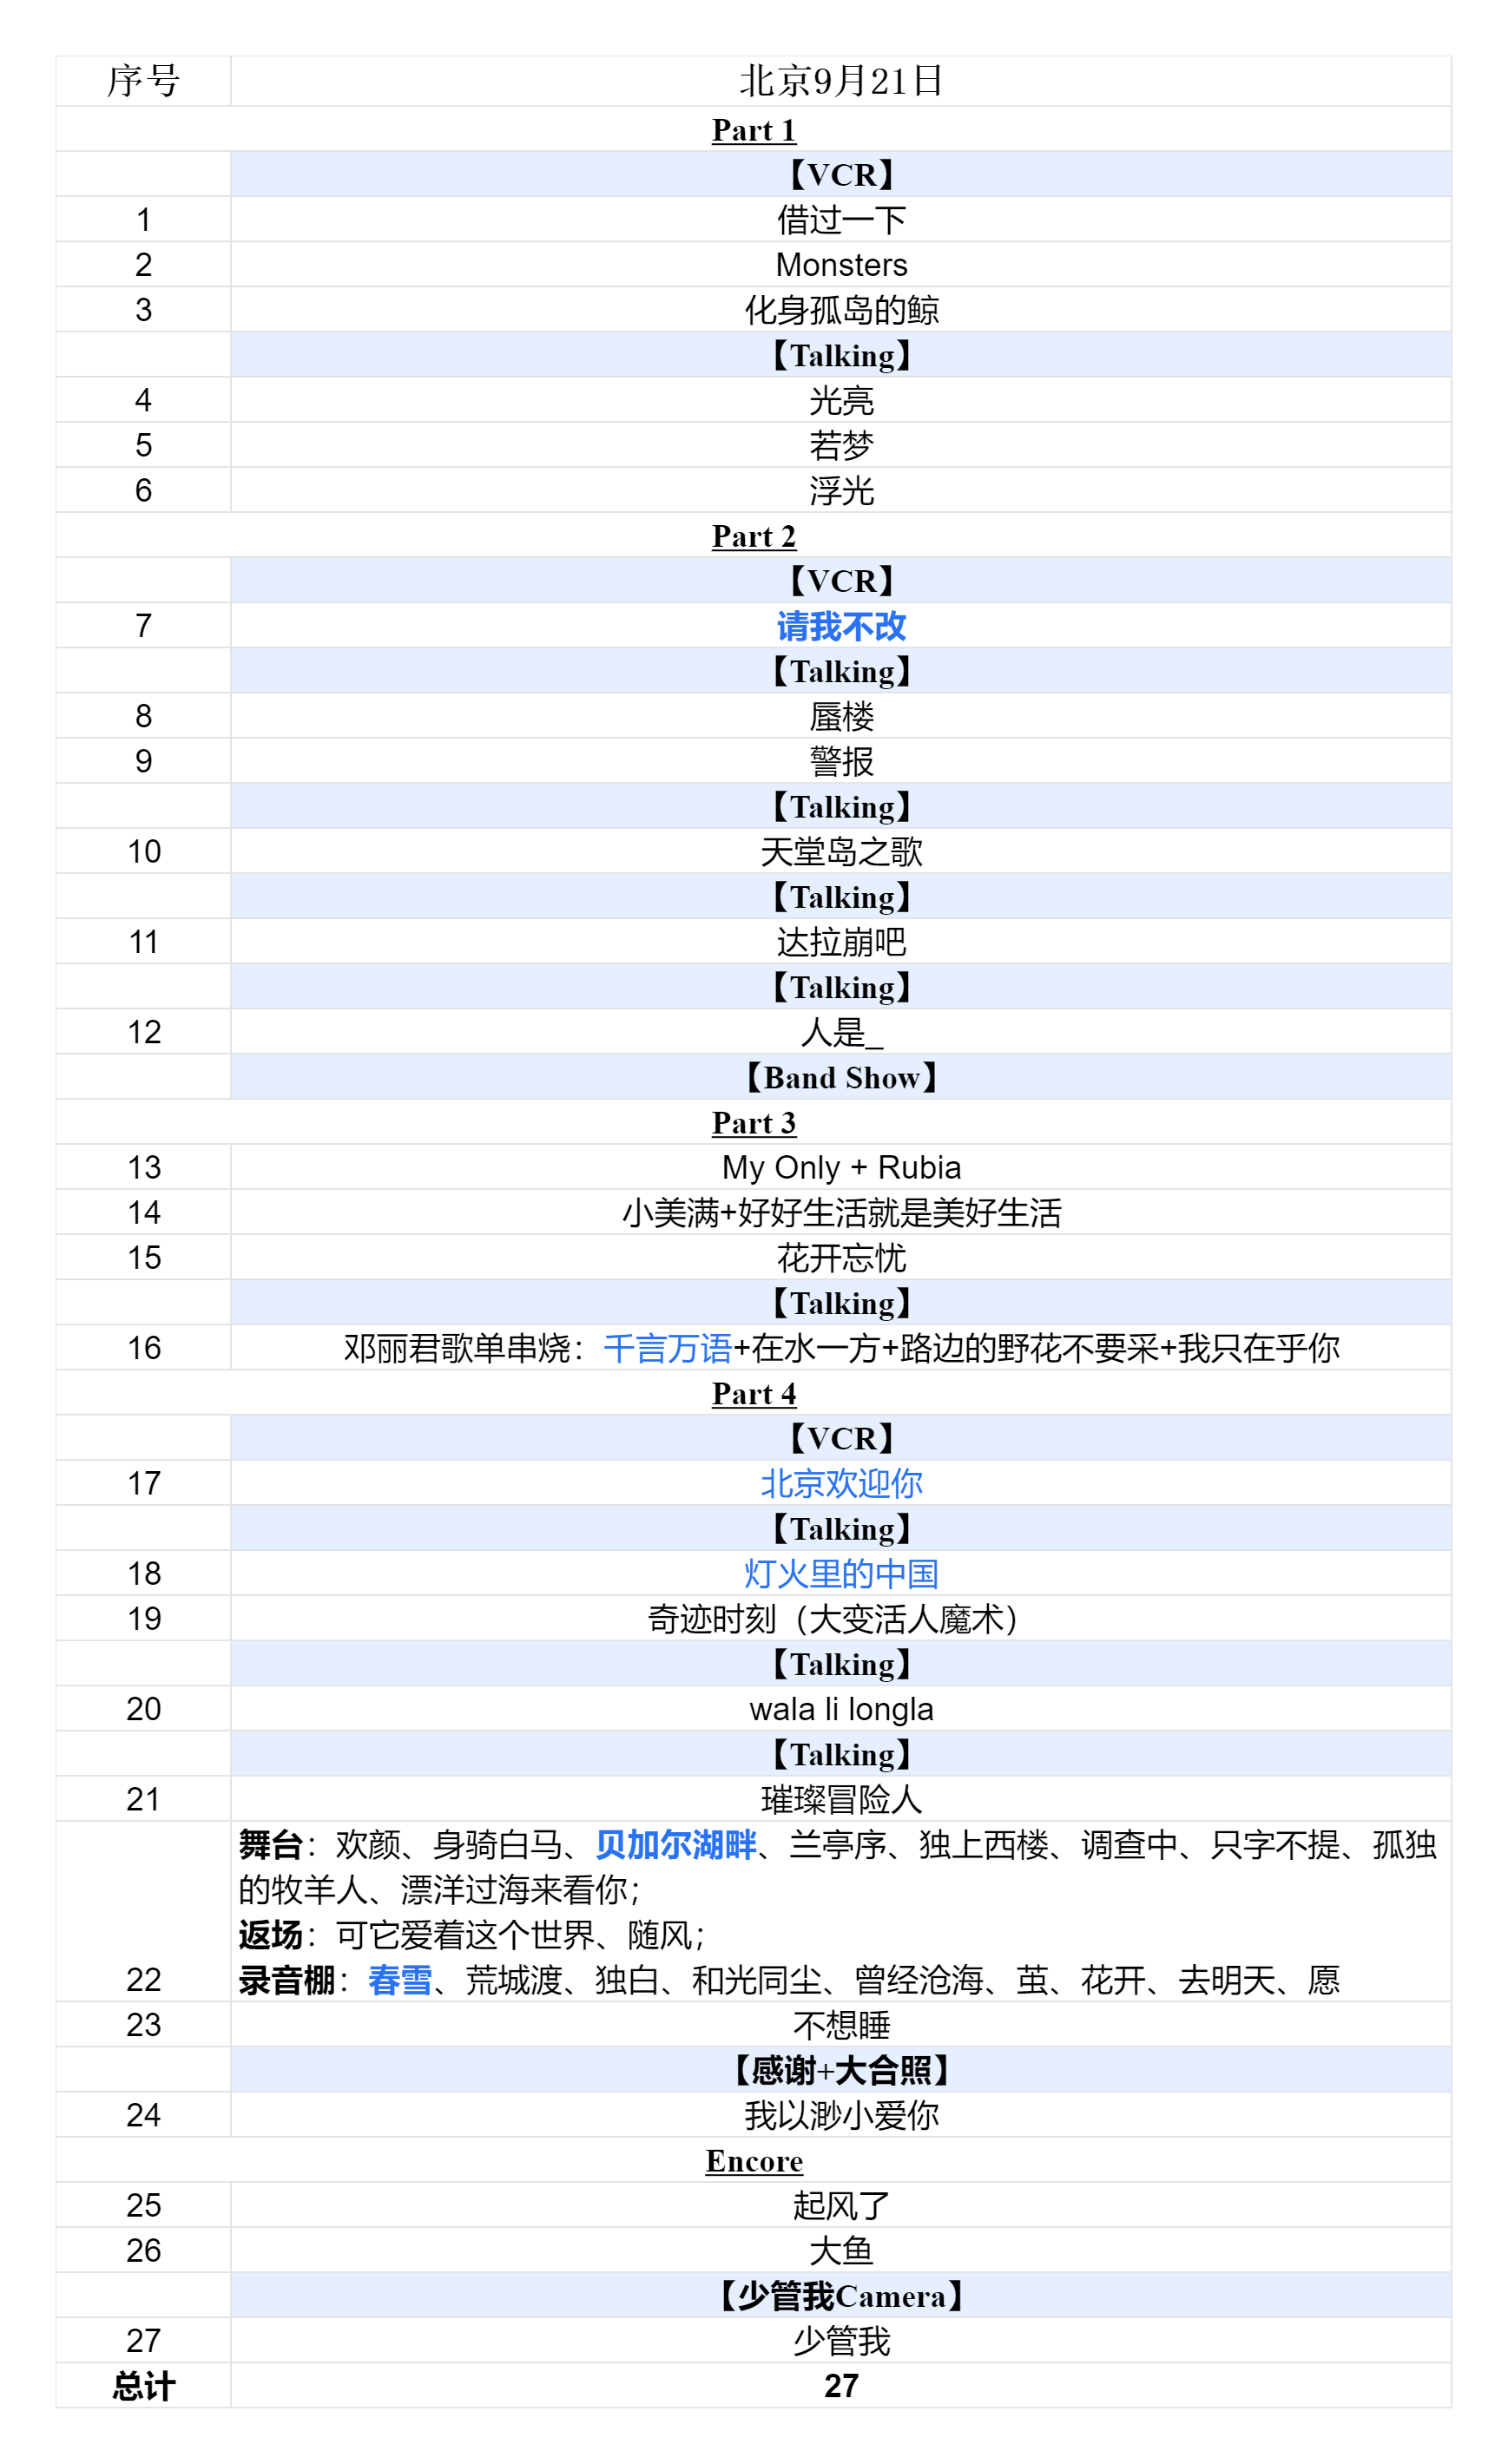
\includegraphics[width=300pt]{img/playlists/playlists-beijing-20240921} 

}

\caption{2024周深9.29Hz巡回演唱会2024.09.21北京第一场歌单}\label{fig:unnamed-chunk-96}
\end{figure}

\newpage

\section{Part1}\label{beijing-20240921-part1}

\hyperref[opening-vcr]{🎥【\textbf{开场VCR}】}

\hyperref[I-will-go-my-way]{🎵【\textbf{借过一下}】}鸟巢的朋友们,你们好吗?

\hyperref[Monsters]{🎵【\textbf{Monsters}】}

\hyperref[hua-shen-gu-dao-de-jing]{🎵【\textbf{化身孤岛的鲸}】}你们会唱这首歌吗?(米:会)那等下愿意跟我一起唱吗?(米:愿意)\textasciitilde 让我听到你们好吗\textasciitilde 看台的朋友\textasciitilde 到你们\textasciitilde 大声点\textasciitilde 看台的朋友\textasciitilde(米:没有墙头)(\textbf{深:无论你们是否有墙头})我不信(深:但是你们仍然是国王王后)谢谢大家\textasciitilde{}

  北京的朋友们,你们好吗?看台的朋友,你们好吗?大家好,我是歌手周深,鸟巢,我们来啦!不知道从什么时候开始,鸟巢好像是每一个歌手就是梦寐以求开演唱会的地方,但是我没有过,因为我觉得这个梦太遥远了,我根本就不敢妄想,谢谢你们。我们的巡演主题叫做9.29Hz,因为人类可以听到的声音是20Hz到20000Hz之间,我觉得我是一个,怎么说呢,很难让大家一下子喜欢的一个歌手,可能需要一点点过程去接纳、去接受,所以就觉得自己很像是9.29Hz这样的存在,但是因为全世界最美好最善良的你们听到了我,为了逐渐去靠近自己的梦想,去到自己很多很多没有想过的地方,就比如像鸟巢。\textbf{谢谢每一个听过我的人,谢谢我的生米,你们把我带到鸟巢了,我们来到鸟巢了。}你们每一次都说我好像给你们光亮,但其实你们才是我的光亮,谢谢你们\textasciitilde{}

\hyperref[silver-linings]{🎵【\textbf{光亮}】}谢谢你们的光亮,\textbf{\textcolor{red}{我爱你们~} } 后面的朋友\textasciitilde{}

\hyperref[ruomeng]{🎵【\textbf{若梦}】}(深深在表演弹琴)每次遇到你们都像一场梦一样,你们愿意跟我一起唱这首若梦吗?(米:愿意)你们唱的是我最爱的版本,我们一起唱哦等下\textasciitilde 到你们喽\textasciitilde 看台的朋友大声点\textasciitilde 太好听啦\textasciitilde 你们唱得太好听啦,这边朋友也要大声唱哦\textasciitilde 最大的声音\textasciitilde 看台的朋友\textasciitilde 全场的朋友一起\textasciitilde(深:唯愿你你你你你你\ldots\ldots 你你能得到拯救)\textbf{因为你们,我才得到你的拯救\textasciitilde{}}

\hyperref[floating-light]{🎵【\textbf{浮光}】}在这人生恍惚三万天当中,遇到的你们,就是我最美的浮光\textasciitilde 跟我一起\textasciitilde 你们\textasciitilde{}

\section{Part2}\label{beijing-20240921-part2}

\hyperref[senself-vcr]{🎥【\textbf{反深代词VCR}】}

\hyperref[brave-heart]{🎵【\textbf{请我不改}】}谢谢你们\textasciitilde{}

  这样的周深,你们感觉陌生吗?有没有吓到你们,刚才大家队都有没有摇起来?(米:有)谢谢你们。第一部分的歌是大家可能比较熟悉的周深,比较古风啊、比较飘渺的。那,应该算是时隔7年,我出了一张专辑叫做(米:反深代词),里面有12个不同的碎片的周深,那我们看一下还有什么样的碎片呢\textasciitilde{}

\hyperref[mirage]{🎵【\textbf{蜃楼}】}

\hyperref[the-giver]{🎵【\textbf{警报}】}

  谢谢大家愿意抽出时间听刚才新专辑的歌,你们喜欢吗?(米:喜欢)谢谢你们,因为我一开始我其实真的真的,我真的真的是个很内向的人。(米狂笑)笑这么大声真的很不礼貌朋友们,但是因为遇到了大家,宝你个头,但是\textbf{因为遇到了大家,我开始有安全感去介绍,就是另外一面的周深,或者说是更加立体的周深给大家认识。}刚才的第一首歌叫做请我不改,对不对,那在什么时候,最近几年有一个词非常有名,叫做PUA,但是很多时候大家忘了,很多时候自己会对自己过于苛责,也是一种自我PUA。就像歌词里面说的一样,很多时候你发现,啊,气压已经压到你无法呼吸的时候,那个追兵和逃兵其实是你自己。所以我们要爱自己,要做好自己,有的时候也要放过自己,好不好?蜃楼是由执念组成的一个蜃楼,有的人因为好的执念能让自己变得越来越好,但有的人却困在那个执念当中,觉得,啊啊啊啊我不开心,但是就像突然就听到了一声警报一样,是刚才的最后一首歌,提醒每一个照顾全世界,照顾所有周围所有朋友的你,也要先好好的爱好自己。你们收到这个警报了吗?答应我要好好的爱自己好吗?看台的朋友没有听到你们的声音哦。没错,很开心可以有很多机会被大家听到,因为我也经常会看到,就是有人说,唉,综艺里面有一个周深,唱歌的里面有一个周深,他们是同一个周深吗?哈哈哈,我很开心,我想告诉你,没错,他们就是同一个周深,我也很开心可以在很多的综艺当中被大家听见,所以你们好,我是歌手周深,你们好吗?今天我们有近6万的观众,让我听到你们的呼喊声。(米狂欢)\textbf{哇,我太幸福了,我太幸福了,}那他们都说我,我不知道哦,就是他们说在演唱会当中指哪里,哪里就会有非常热烈的呼喊声,是真的吗?那如果是这样呢?这样呢?这样呢?那如果我指看台的朋友呢?(米狂欢)哇,好像感觉近6万的朋友应该声音更大,那我试试这样呢?你们太美好了,谢谢你们。最后我想郑重的说四个字,宝你个头,但是\textbf{\textcolor{red}{我爱你们} }。原来在鸟巢唱歌是这种感觉,你们觉得我的声音好听吗?(米:好听)哇,那我们再听一下,是什么吧\textasciitilde{}

\hyperref[haven-song]{🎵【\textbf{天堂岛之歌}】}谢谢\textasciitilde{}

  接下来要到你们唱歌的时候喽,有一个童话故事呀,有个童话故事呀,最难记的就是他的主角的名字,我们来考一下啊。主人翁的名字叫做达拉,(米:达拉崩吧斑得贝迪卜多比鲁翁)哇,你们很厉害,那我考一个偏难一点的,那个公主的名字叫做,公主?(米:米娅莫拉苏娜丹妮谢莉红)你们自己唱吧,那等下一定要唱得更大声哦,看台的朋友听到没有?

\hyperref[dalabengba]{🎵【\textbf{达拉崩吧}】}全场嗨起来\textasciitilde 看台的朋友\textasciitilde 现在又到你们唱的时候哦,想一想,是谁为了拯救谁,打败谁,又回到哪里呢?于是\textasciitilde(米:达拉崩吧斑得贝迪卜多比鲁翁)砍向\textasciitilde(米:昆图库塔卡提考特苏瓦西拉松)然后\textasciitilde(米:昆图库塔卡提考特苏瓦西拉松)咬了\textasciitilde(米:达拉崩吧斑得贝迪卜多比鲁翁)看台的朋友大声点,最后\textasciitilde(米:达拉崩吧斑得贝迪卜多比鲁翁)再来哦,他的名字叫达拉(米:达拉崩吧斑得贝迪卜多比鲁翁)打败了昆图(米:昆图库塔卡提考特苏瓦西拉松)这么爱念哦,(深:要念你来念吧\textasciitilde)谢谢你们,你们觉得好听吗?

  我真的非常非常的珍惜每一次跟大家见面的机会,我也很开心可以遇到很多很多老师去帮我们营造那么好的氛围去见面,我要告诉大家一个,怎么说呢,小秘密或是很可爱的一个话题,哈哈哈,就是我们在搭建,因为鸟巢这么重要的地方,我们就希望大家可以更加的更清楚的听到我们的声音。我们每个地方也都是这么做的,然后直到鸟巢的工作人员告诉我们说,\textbf{老师们,你们不能够再加音响了,快要超过鸟巢可以承重的那个音响的重量了,}哈哈哈,你们觉得你们听得开心吗?谢谢你们,我也很开心可以来到鸟巢给大家唱歌。那这首歌希望你们能够喜欢,人是\_

\hyperref[renshi]{🎵【\textbf{人是\_}】}你们好吗\textasciitilde 谢谢你们\textasciitilde{}

\section{Part3}\label{beijing-20240921-part3}

  大家好,你们看到我在哪了吗?唔\textasciitilde 因为北京有点凉快,你们都有好好的加衣服吗?(米:有)我也有哦,秋衣,大家也要听爸爸妈妈的话,或者是听\textasciitilde 话\textasciitilde,要记得多添加衣服,你们有穿好吗?(米:有)接下来两首歌我觉得是,非常浪漫,非常温暖,就像秋衣一样。其实想告诉大家,就是如果你想学习任何一个技能,什么时候开始都不晚。我也不是从小就开始学唱歌,当然学琴,你们一听也知道,哈哈哈,开始的比较晚,但是没有关系,只要你喜欢的事情,随时都可以开始好吗?(米:好)希望大家能够喜欢这两首歌。如果等下弹的不好能够给我鼓励吗?(米:能)我先听一下。唉,气势起得这么好,等下弹得不好真的怎么办?哎,为什么我的这个踏板没有声音?救命啊,踏板没有声音,哇哦哇哦哇哦,人生真是充满惊喜儿,哈哈哈,来到北京我就发现说儿化音对我们南方人特别难。这个钢,这句话应该怎么加儿化音?钢琴踏板没有声音,钢琴儿踏板儿,哈哈哈,那个钢琴儿踏板儿还是没有声,先这样吧\textasciitilde{}

\hyperref[my-only]{🎵【\textbf{My Only}】} \hyperref[rubia]{🎵【\textbf{Rubia}】}啊\textasciitilde 没有人救我是吗?好,重来一遍\textasciitilde(深唱:你真的好努力,你帮我处理事情)我们掌声先给他\textasciitilde(深:to find the way 宝你们个头)

\hyperref[happy-ending]{🎵【\textbf{小美满}】}要跟我一起大声唱哦,要超大声,来\textasciitilde 跟我一起\textasciitilde{}\textbf{你们是世界上最美好的存在哦},再大声点唱\textasciitilde 唱,看台的朋友\textasciitilde(岁月很长\textasciitilde)岁月很长,慢慢来\textasciitilde 谢谢你们\textasciitilde 大家喜欢这首小美满吗(米:喜欢)我也很喜欢,就每次唱这首歌我就觉得是很幸福,感觉所有的愿望都可以实现。我们不如就在这首歌当中一起许愿吧,好不好?我先做个例子哦,我们闭上眼睛,默默许下心中想要许的那个愿望,然后321睁开眼睛,我们的愿望就会挂在这棵树许愿树上面。所以现在无论你是多大的年纪,无论你是做什么职业的人,现在请跟我们一起闭上眼睛,默默许个愿望,好不好?来,看台的朋友,所有的朋友,闭上眼睛,心中想一想你要许的愿意,它很神奇的,它真的会实现的哟。默默想好这个愿望,哎呀,我忘记了一个事情要说,这个愿望只能够许关于自己的愿望,想一想有多久没有关心过自己,有多久没有给自己个拥抱呢,三二一\textasciitilde 你们的愿望都被听到啦\textasciitilde{}

  一定要像小美满这首歌一样,好好爱自己,好好爱自己,才是所有美好的开始好不好?

\hyperref[live-happy-life-happy]{🎵【\textbf{好好生活就是美好生活}】}

\hyperref[no-worries]{🎵【\textbf{花开忘忧}】}(米:你好啊)你好啊\textasciitilde{}\textbf{北京的朋友,我们来你们的家玩喽,我们来看你们呐\textasciitilde{}}愿意跟我一起唱吗\textasciitilde 你们\textasciitilde 我们的思念他们一定听得见,对不对?(米:对)花开忘忧,愿你无忧,花开忘忧,(米:愿你无忧)谢谢你,谢谢你们\textasciitilde{}

  我很好奇的是,你们是什么时候开始听我唱歌的啊?我刚才看到有,已经听了八年。哎呀,我刚才有看到说听了8年的,然后是不是有?会不会有更长时间的?有没有是今年第一年开始听我唱歌的?那有没有人是第一次来到鸟巢的呢?你们真的太厉害了,因为你们把我也带到鸟巢喽。唔\textasciitilde 这里真的是我从来没有想过自己能够来开演唱会的人,甚至就连做个梦都不敢梦见自己在鸟巢开演唱会。所以你们真的太厉害了。第一次让我感受到什么是唱歌的歌手叫做邓丽君女士。我觉得,第一次听到就觉得,哇太好听了,原来还有另外一种方式去说话,我也希望自己可以成为像邓丽君女士一样的歌手,无论过了多少年,还是会有人记住她,她的歌当中也存放了很多人的记忆。你们听过她的歌吗?(米:听过)那等一下跟我一起唱哦,看台的朋友。宝你个头\textasciitilde{}

🎵【\textbf{邓丽君组曲}】
\hyperref[thousands-of-words]{🎵【\textbf{千言万语}】}(深:那天起,你对我说,永远的爱着我)骗子(深:千言和万语,随浮云掠过)啊,受伤了\textasciitilde{}
\hyperref[on-the-water-side]{🎵【\textbf{在水一方}】}大家跟我一起唱哦\textasciitilde 到你们\textasciitilde{}
\hyperref[walk-the-road-of-life]{🎵【\textbf{路边的野花不要采}】}有墙头的人听好了(深:路边的野花)你们告诉他(米:你不要采)听到了没有,听听劝吧,哎呀\textasciitilde 你们会把我忘记吗?(米:不会)\textbf{我只在乎你!}
\hyperref[only-you]{🎵【\textbf{我只在乎你}】}看台的朋友\textasciitilde 大声点\textasciitilde 看台的朋友\textasciitilde 谢谢你们看到了我\textasciitilde{}

\newpage

\section{Part4}\label{beijing-20240921-part4}

\hyperref[thank-you-vcr]{🎥【\textbf{谢谢北京,谢谢你VCR}】}

\begin{figure}

{\centering 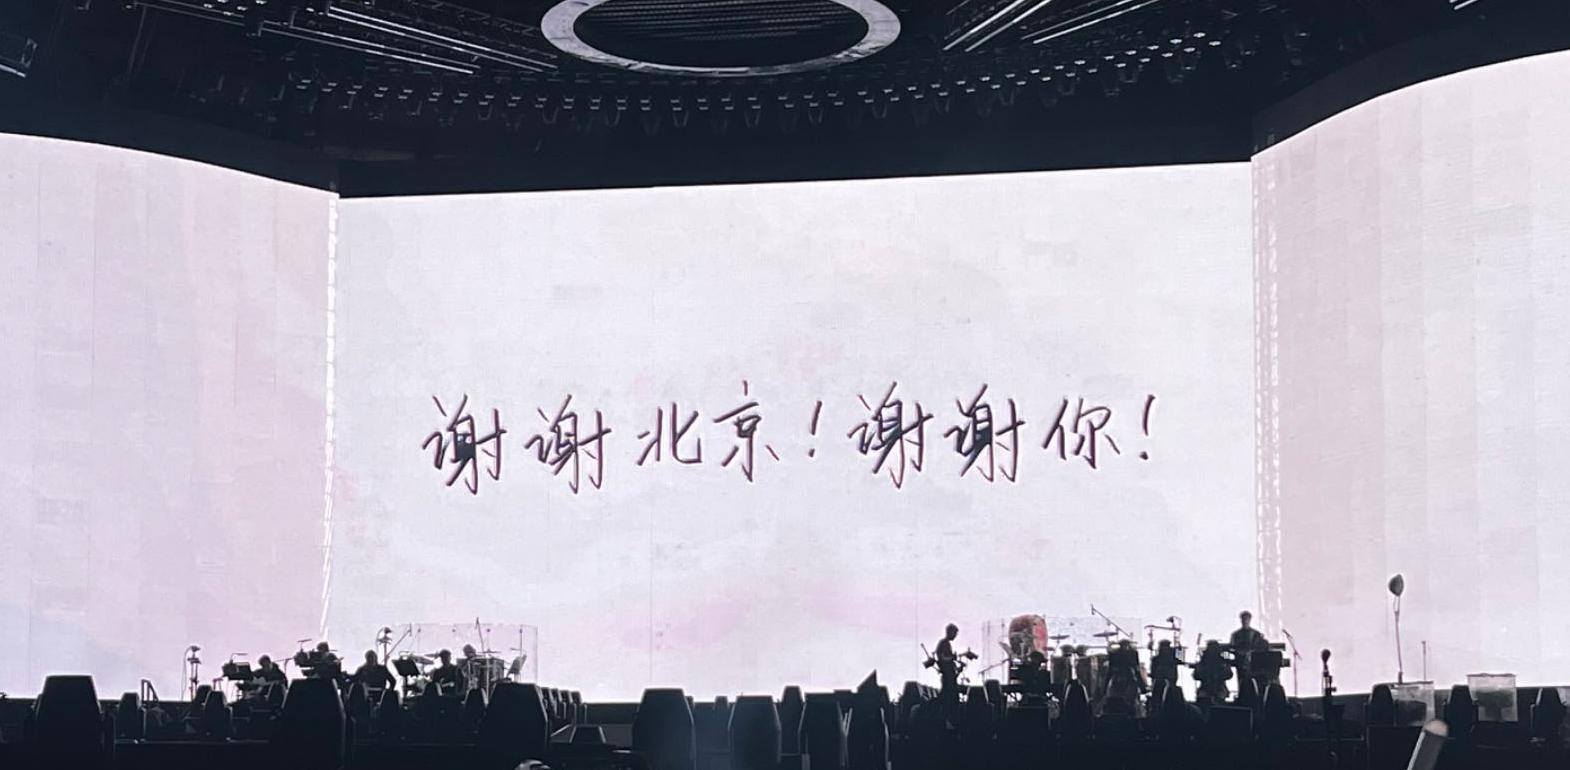
\includegraphics[width=400pt]{img/beijing20240921/thank-beijing} 

}

\caption{谢谢北京!谢谢你!}\label{fig:unnamed-chunk-97}
\end{figure}

  朋友们,你们好吗?北京鸟巢,我们来了。大家还记不记得,就是08年奥运的时候,当时的你在干什么呀?噢,我非常清楚的记得08年的时候我还在贵阳的那个就是我们有个广场,会有个公共的大屏幕,所以我是跟很多同学们以及我们很多的贵阳的朋友们一起去看的那个开幕式。当时我就觉得,哇,我要是能够在北京欢迎你里面唱一句,那得多厉害哇。那个时候的我,那个时候的周深依然是写不出以我的梦想为题的作文,因为我从小不知道自己会成为什么样的人。或是也不知道自己比较擅长什么事情,但是我没有想到就当年那么一句妄想,能够在16年之后,因为你们把我带到了鸟巢。我没有想到能够,没有想到自己有一天能够在这里给大家唱歌,然后我也听说这个好像是北京欢迎你这首歌第二次在鸟巢响起,等一下你们愿意跟我一起唱吗?(米:愿意)还有一个最美好的事情,就是当年奥运会开幕式的音响总监金少刚老师,也是我们今天演唱会的音响总监。我觉得我们真的像歌里面唱的一样,我们有梦想,我们真的很了不起,我们有勇气一定可以创造奇迹。其实我也经常在想,就是,诶,鸟巢它的特别之处在哪里呢?它也是一个体育场,但是我彩排的时候我发现我一切都知道了。我一直都明白为什么所有的歌手都很想在这里开演唱会,因为鸟巢这里是我们中国人创造了非常非常多奇迹的地方,是我们的骄傲,是我们的底气,所以一起跟我唱这首北京欢迎你,好吗?(米:好)谢谢你们。

\hyperref[welcome-to-beijing]{🎵【\textbf{北京欢迎你}】}一起\textasciitilde 来啰\textasciitilde(北京欢迎你\ldots)大声点\textasciitilde 请相信自己,努力的向前冲,好不好?(米:好)但是也要记得好好的爱自己。答应我好吗?(米:好)再来\textasciitilde 看台的朋友\textasciitilde 大声点\textasciitilde 再来一遍\textasciitilde 看台的朋友大声点\textasciitilde{}

\hyperref[China-in-the-light]{🎵【\textbf{灯火里的中国}】}然后这个普普通通的小男孩登上了春晚,这都是你们创造的奇迹,所以相信自己非常强大,好吗?(米:好)等一下你们愿意跟我一起大声唱吗\textasciitilde 一起\textasciitilde 全场\textasciitilde(灯火里的中国青春婀娜)大声点\textasciitilde 谢谢大家\textasciitilde{}

  你们把一个非常普通的小男孩,让他慢慢慢慢去靠近他的梦想了,这怎么能够说不是一个奇迹时刻\textasciitilde{}

\hyperref[magic-moment]{🎵【\textbf{奇迹时刻}】}(米:宝贝)宝你个头,宝你个头,看台的朋友,宝你们的头\textasciitilde 呦吼,现在睁大你们的眼睛看清楚\textasciitilde【大变活人魔术】

  你们喜欢吗?还想要耽误大家一点时间听一下反深代词里面的歌,但是它是一个快乐密码,这个密码叫做wala li longla,你们可以跟我学一下哦,wala(米:wala),看台的朋友大声点哦,wala li(米:wala li),wala li long(米:wala li long),wala li longla(米:wala li longla),只要念响这个密码,快乐永远都会跟着你哦\textasciitilde{}

\begin{figure}

{\centering 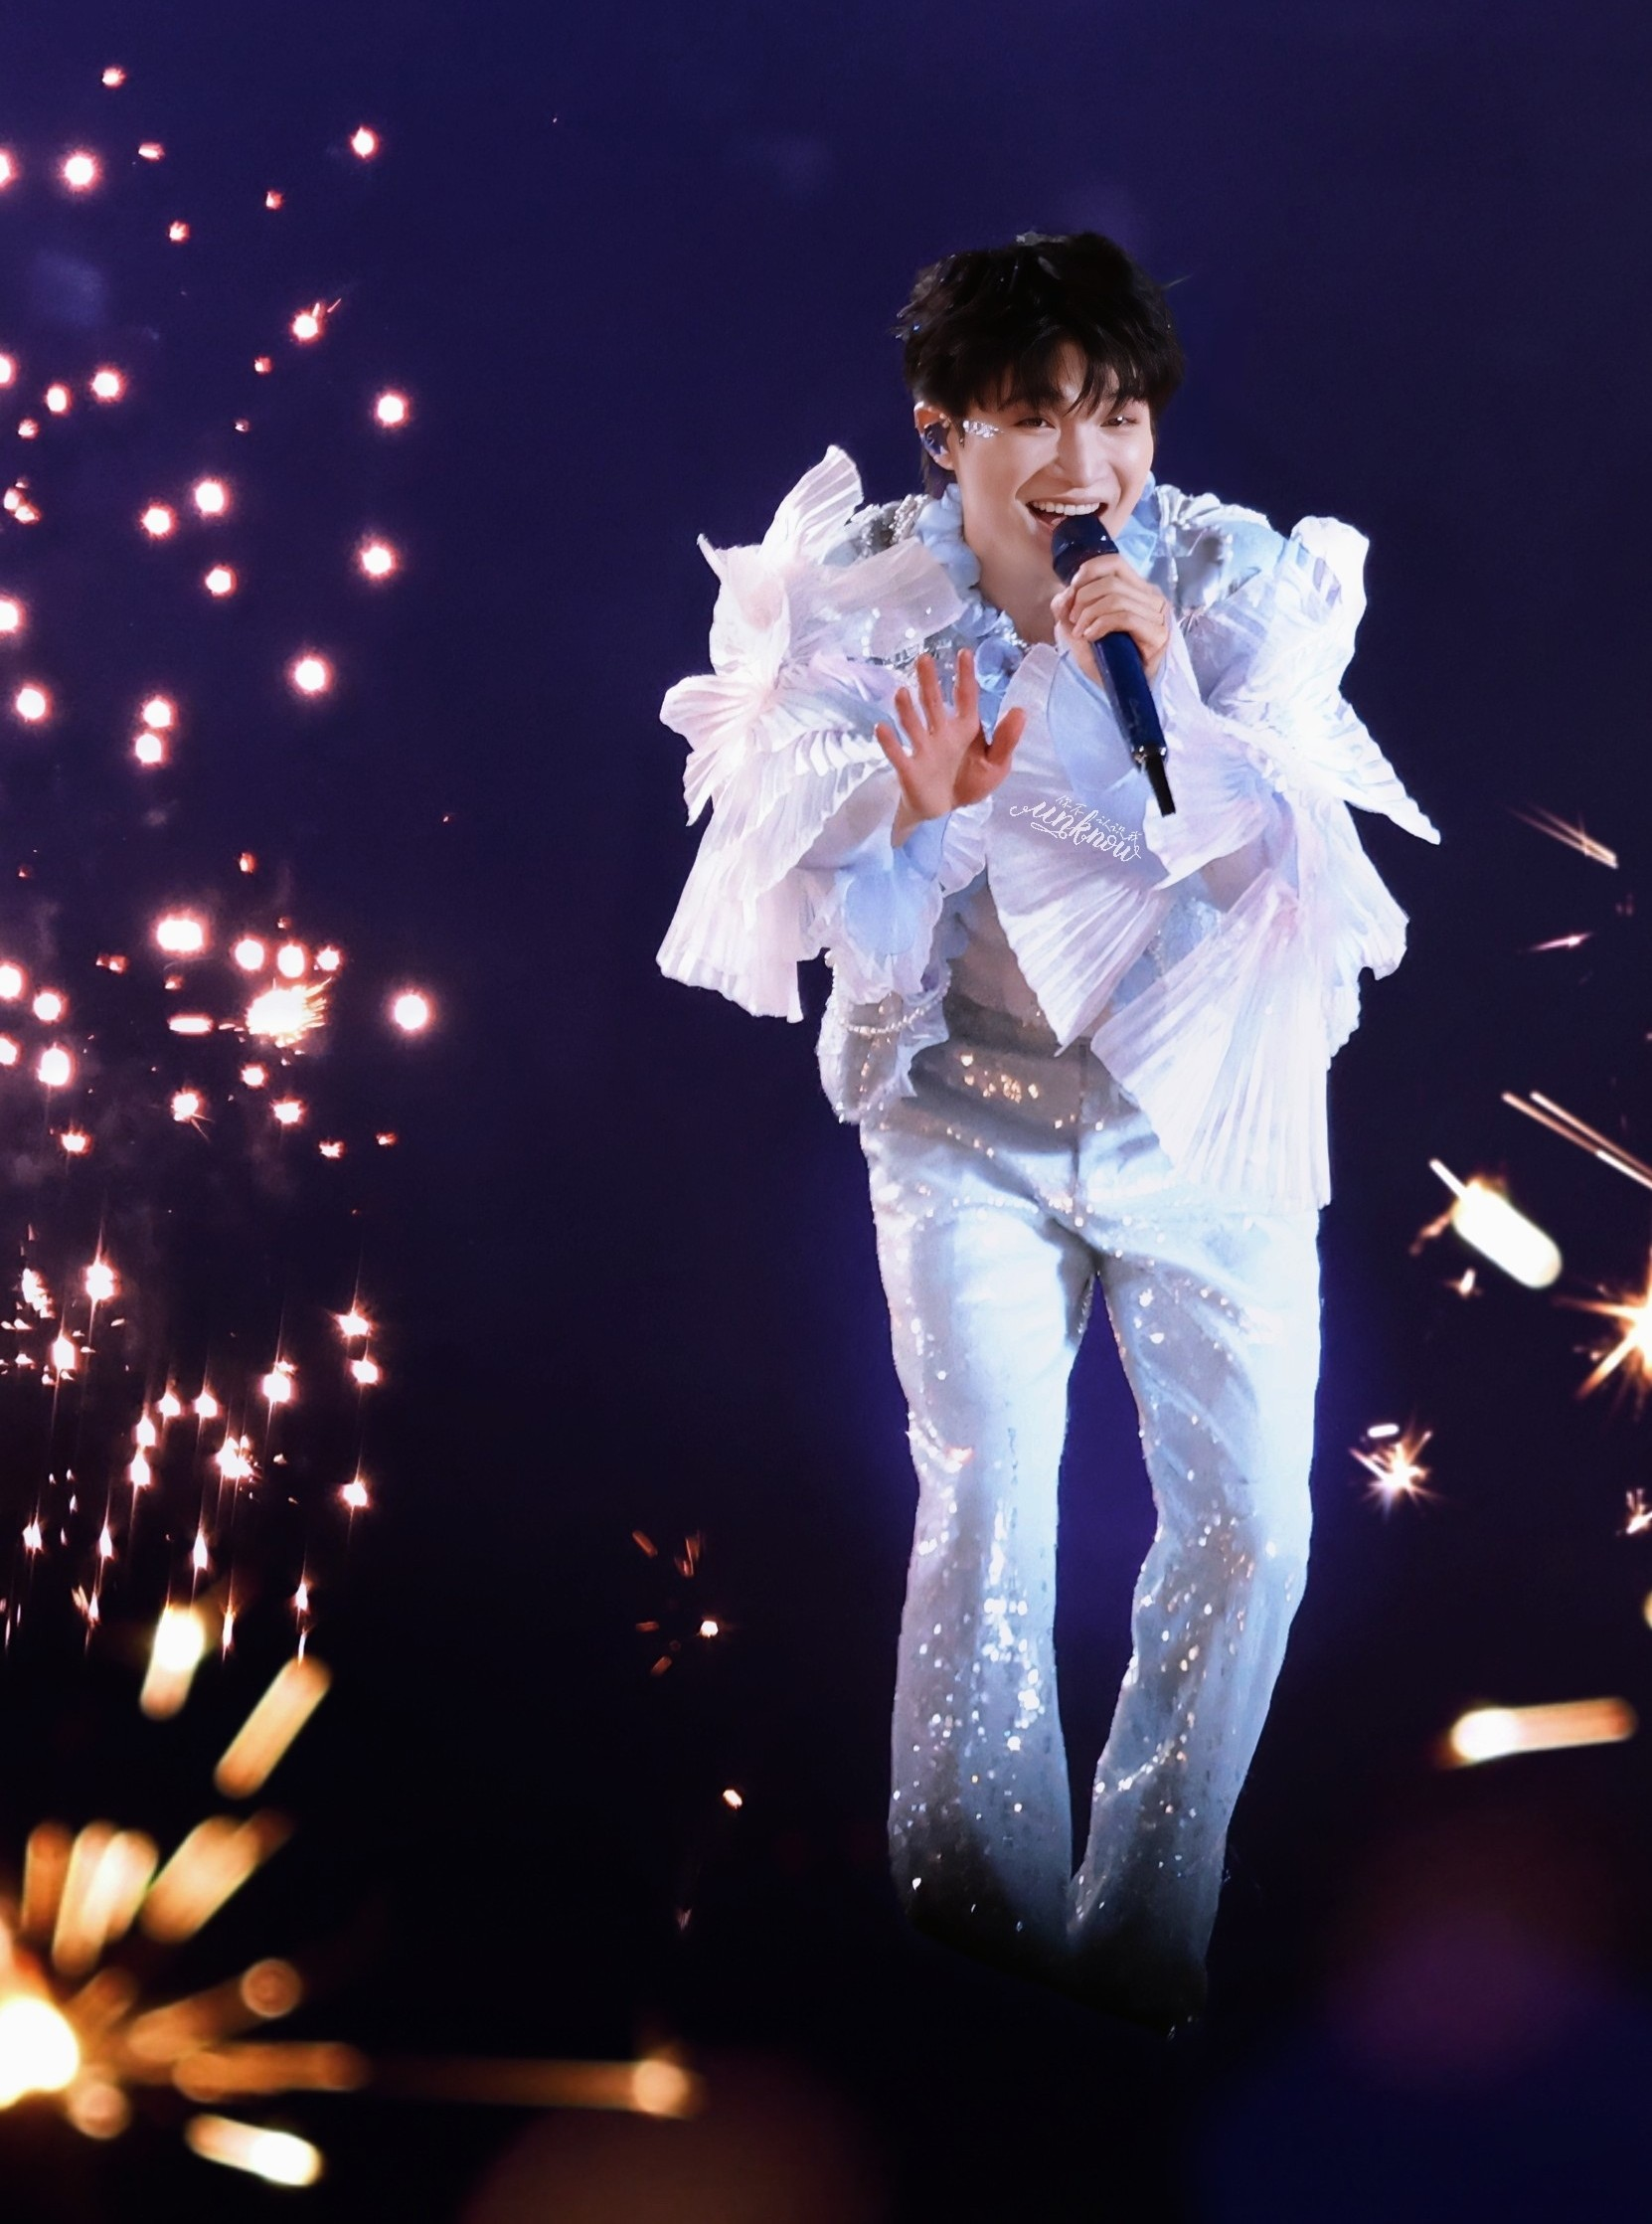
\includegraphics[width=450pt]{img/beijing20240921/001} 

}

\caption{绝美瞬间!}\label{fig:unnamed-chunk-98}
\end{figure}

\hyperref[wala-li-longla]{🎵【\textbf{wala li longla}】}看台的朋友,你们在吗\textasciitilde(提词器罢工,深:繁星里去涂鸦,找鳄鱼借杯茶\textasciitilde)嗨起来\textasciitilde 看台的朋友也要大声跟我一起默念这个密码,全场好不好?我念一句,你们就跟着我念一句,哦,走,听好\textasciitilde wala,wala li,wala li long,wala li longla\textasciitilde 看台的\textasciitilde 全场\textasciitilde 全场\textasciitilde 全场再来一遍,321\textasciitilde 你们是最棒的\textasciitilde{}

  接下来这首歌呢,它好像今年,oh,非常巧,它好像在今年也配了很多我们奥运健儿们的视频,他非常的热血,非常非常的鼓舞人心。我们的人生其实也很像一场比赛,但是我们是马拉松,我们可以一直,它是很长的一段路,所以不要害怕,这首歌叫做璀璨冒险人。所以呢,\textbf{不要害怕失败,不要害怕被打败,我们都是璀璨冒险人,对不对?(米:对)我们一定会收获属于我们的璀璨的\textasciitilde{}}

\hyperref[adventurers]{🎵【\textbf{璀璨冒险人}】}(深:这一路光景,有你在身旁)全场跟我一起\textasciitilde(他们说要越过前方风沙必须低着头\ldots\ldots)大声点\textasciitilde{}\textbf{你们都是最棒的\textasciitilde{}}全场\textasciitilde(米:还想要继续吗)要,(米:要逆风不退啊\textasciitilde)(深:不惧脆弱)我们都(深:不惧脆弱\textasciitilde)谢谢大家\textasciitilde{}

【\textbf{点歌环节}】现在呢,到我们9.29Hz的点歌时间啦,从我们鸟巢站开始,点歌他换了一种方式,我很开心自己用,应该是说在各个地方唱的歌被大家听到,有在像录音棚,也有的像在舞台上。有哪些人是听我深的深的歌认识的我的?有哪些人是听反深代词认识我的?那有没有人是听蒙面唱将猜猜猜里面的?(米:有)是有哦。那有没有人是看我出道的时候听到的歌手周深的?所以我很珍惜每一个被你们听到的机会,我们从现在开始就是点歌会变成要点两个人。但是每首歌点出来之后只能唱一半哦。全场跟我倒数5个数字好不好?全场(米:54321),停,你在哪里?你生日,生日快乐。哎呦,这里是不是生日快乐?今天生日的你,生日快乐,我们全场祝今天生日的人(米:生日快乐)那么噢,你在这里啊,对不起,哈哈哈,居然这么近,你好怎么称呼?(你可以叫我橙子)哦,那你这个橙子甜不甜呢?(甜)甜,哈哈哈,您大概什么时候开始听我唱歌的啊?(从2020年开始)哦,2020年,那也四年了,你很厉害。你听我的第一首歌是(大鱼)哦,大鱼,好,我们来看一下吧。我们现在有两个选择,一个是舞台,舞台就是,比如看像贝加尔湖畔啊,兰亭序啊,漂洋过海来看你,这都是我在舞台上唱的一些可能别人的作品,录音棚就是我在录音棚录制的作品啦。我在解释了什么呢?我也不知道,哈哈哈。然后中间两首是之前点歌有唱过的,看一下有没有你喜欢的歌。(有)你是来自哪里的朋友?(我来自北京),你就是北京当地人。您教我说一句最地道的北京话。(我不是老北京人)那来选歌吧,你想听哪首?(我想听春雪,非常喜欢这首歌。我觉得这首歌非常的有特色,然后非常的细腻,温柔)你给我这么一本正经的回答,哈哈哈哈,我都感觉我们在参与就是论文的答辩。来讲这首歌是什么风格,用了什么样的配器,他想表达的是什么情感,交给你了。哈哈哈好,谢谢全场最甜的橙子,谢谢你,那这首春雪希望你们喜欢哦\textasciitilde{}

\begin{table}

\caption{\label{tab:unnamed-chunk-99}2024周深9.29Hz巡回演唱会09.21北京场点歌歌单}
\centering
\begin{tabular}[t]{lll}
\toprule
舞台 & 返场 & 录音棚\\
\midrule
1-欢颜 & 1-可它爱着这个世界 & 1-春雪\\
2-身骑白马 & 2-随风 & 2-荒城渡\\
3-贝加尔湖畔 &  & 3-独白\\
4-兰亭序 &  & 4-和光同尘\\
5-漂洋过海来看你 &  & 5-曾经沧海\\
\addlinespace
6-独上西楼 &  & 6-茧\\
7-只字不提 &  & 7-花开\\
8-孤独的牧羊人 &  & 8-去明天\\
9-调查中 &  & 9-愿\\
\bottomrule
\end{tabular}
\end{table}

\hyperref[spring-snow]{🎵【\textbf{春雪}】}全场\textasciitilde 全场摇起来\textasciitilde 你们觉得好听吗(米:好听)谢谢你们,谢谢橙子,希望大家能够喜欢这首春雪\textasciitilde{}

  全场再一次倒数五个数字,5(米:4321)你在哪里?您好,怎么称呼您?(朋友都叫我雪,下雪的雪)雪(宝贝,你好)宝你个头。那你这个名字叫起来很文艺,你想一想,就是如果我要借个橡皮擦,雪,你的橡皮擦借我一下好吗?雪,今天所有的雪花都汇聚成了你,(太棒了)。雪,你是来自哪里的雪,等一下,只叫一个人的名字,只叫一个字真的很奇怪。哈哈哈,(真的)有没有两个字的称呼,(雪真)什么?(雪真)哦?雪真。你好,你是来自哪里的?(台北)你好,欢迎你来哦。那你听我的第一首歌是?(愿得一人,一心人)是看剧的时候认识我的,对不对?(我先听到歌)哦,谢谢你,那您看一下有没有你想听的歌呢,也没有愿得一心人,(但我来之前我许愿了胡同少年,但没有这首)我在这儿给你道歉(我想听贝加尔湖畔)谢谢你,谢谢雪,谢谢雪真(谢谢周深)有多少人是通过这首歌听过我的声音的?我非常感谢这首歌的创作者李健老师,希望大家能够喜欢这首贝加尔湖畔\textasciitilde{}

\hyperref[lake-baikal]{🎵【\textbf{贝加尔湖畔}】}谢谢,谢谢我们来自中国台北的雪,也希望大家能够玩的开心。你们今天玩的开心吗?(米:开心)谢谢你们\textasciitilde{}

\hyperref[keep-playing]{🎵【\textbf{不想睡}】}到你们\textasciitilde 你们太棒啦\textasciitilde 你们知道吗?你们手电筒发射出来的光子会在宇宙的很远处,很多年之后我们就再一次相遇了\textasciitilde 全场\textasciitilde 全场\textasciitilde 你们是最棒的\textasciitilde 谢谢大家\textasciitilde{}

  大家今天听得开心吗?(米:开心)\textbf{我看到好多人都好漂亮好帅气哦,好棒啊,谢谢你们。}当然我们也要非常感谢所有为我们创造这样一个非常开心,然后一起见面的机会,对不对?谢谢你们,你们的那个手电筒,稍微收一下喽,要不我害怕等一下没有电了,没办法打车。好,那我们一起来感谢场地支持,国家体育场鸟巢,鸟巢我们来了哟,感谢本次巡演全程主办北京时代立方文化传播有限公司,感谢演唱会制作单位必应,感谢我们的总导演周佑洋,庄惟惞,以及音响总监金少刚。谢谢大家,谢谢师傅,谢谢少刚老师,然后也感谢我们的音乐总监龙隆老师,感谢我们今天的乐队老师们。掌声再热烈一点,也谢谢我们的合唱老师们,感谢我们的舞蹈团队,感谢SDT showPro,感谢服装团队,也就是设计师劳伦斯·许工作室,谢谢时装品牌Windowsen,谢谢我们的音响工程,南京奥斯泰,谢谢调音团队乐尔工作室。谢谢硬体工程北京立超舞台集团,谢谢周深工作室的小伙伴们,谢谢大家,谢谢,我们会继续努力的,也要感谢我们的志愿者们。当然要感谢我们的北京,非常感谢北京这座城市,也要感谢我们北京的公安、文化、消防、应急等所有职能部门的大力支持,保障我们这场演出的顺利进行。再大声一点,感谢他们。感谢我们所有台前幕后的工作人员们,也感谢我们今天现场的安保团队,大家辛苦了,\textbf{当然最重要的要感谢来到现场的每一个你。}

  \textbf{你们真的太美好了},因为随着我出道的时间越来越长,我会发现就一开始我以为,唉,好像是很多一些不太好的评价它消失了,其实并不是的,那些不太好的评价或者是故意伤害的东西它依然存在。但是我听到了你们又温暖又炙热的爱的声音,所以我觉得我都不害怕了,谢谢你们,\textbf{也希望你们可以把今天这场演唱会当作一颗非常甜的回忆里的糖,当你需要的时候,它都会给你力量,好吗?}(米:好)记住那句话,好好爱自己。(米:好)

  我们来合照吧。(米:好)那我们中间哦,321,这边。来,321,这边哇,321,看台的朋友,我来喽\textasciitilde(深深跟摄影师在左右抉择上不同)真的很没有默契,哈哈哈,你们好,要注意安全哟,安全第一哟。来吧,3,321,这边的朋友,3,宝你个头,321,那边的朋友来喽,鸟巢真的好大呀。(米:加油加油),你们为我加油,我以为我在参加运动会,321,这边的朋友,你们好吗?321,谢谢老师,谢谢你们。

  刚才的不想睡是卡布的一首晚安曲。那接下来要演唱的是周深的晚安曲,叫做我以渺小爱你。谢谢你们看到了渺小的我,谢谢你们看到了渺小的我,谢谢你们\textasciitilde{}

\hyperref[loving-you-in-my-humble-way]{🎵【\textbf{我以渺小爱你}】}谢谢生米,也谢谢每一个听过我,给我善意的你。我不知道自己还能够唱多久?还能不能唱高音,但是很开心在这人生恍惚三万天当中有出现在你们的人生当中,谢谢你们听到了我,谢谢你们来,谢谢你们在,(我以短暂爱你不朽的旅程)\textbf{\textcolor{red}{我爱你们~} }

\section{Part5}\label{beijing-20240921-part5}

\hyperref[the-wind-rises]{🎵【\textbf{起风了}】}你们好\textasciitilde 谢谢你们来,谢谢你们还在\textasciitilde 谢谢你们\textasciitilde 以爱之名,你还愿意吗?(米:愿意)看台的朋友,你们好吗\textasciitilde 谢谢你们\textasciitilde{}

\hyperref[big-fish]{🎵【\textbf{大鱼}】}谢谢你们\textasciitilde 我现在就是越来越明白,就是为什么金少刚老师他一直提醒我,就说你真的要好好感谢你的观众们,因为他们真的太棒了,你们真的太棒啦,谢谢你们\textasciitilde{}

\begin{figure}

{\centering 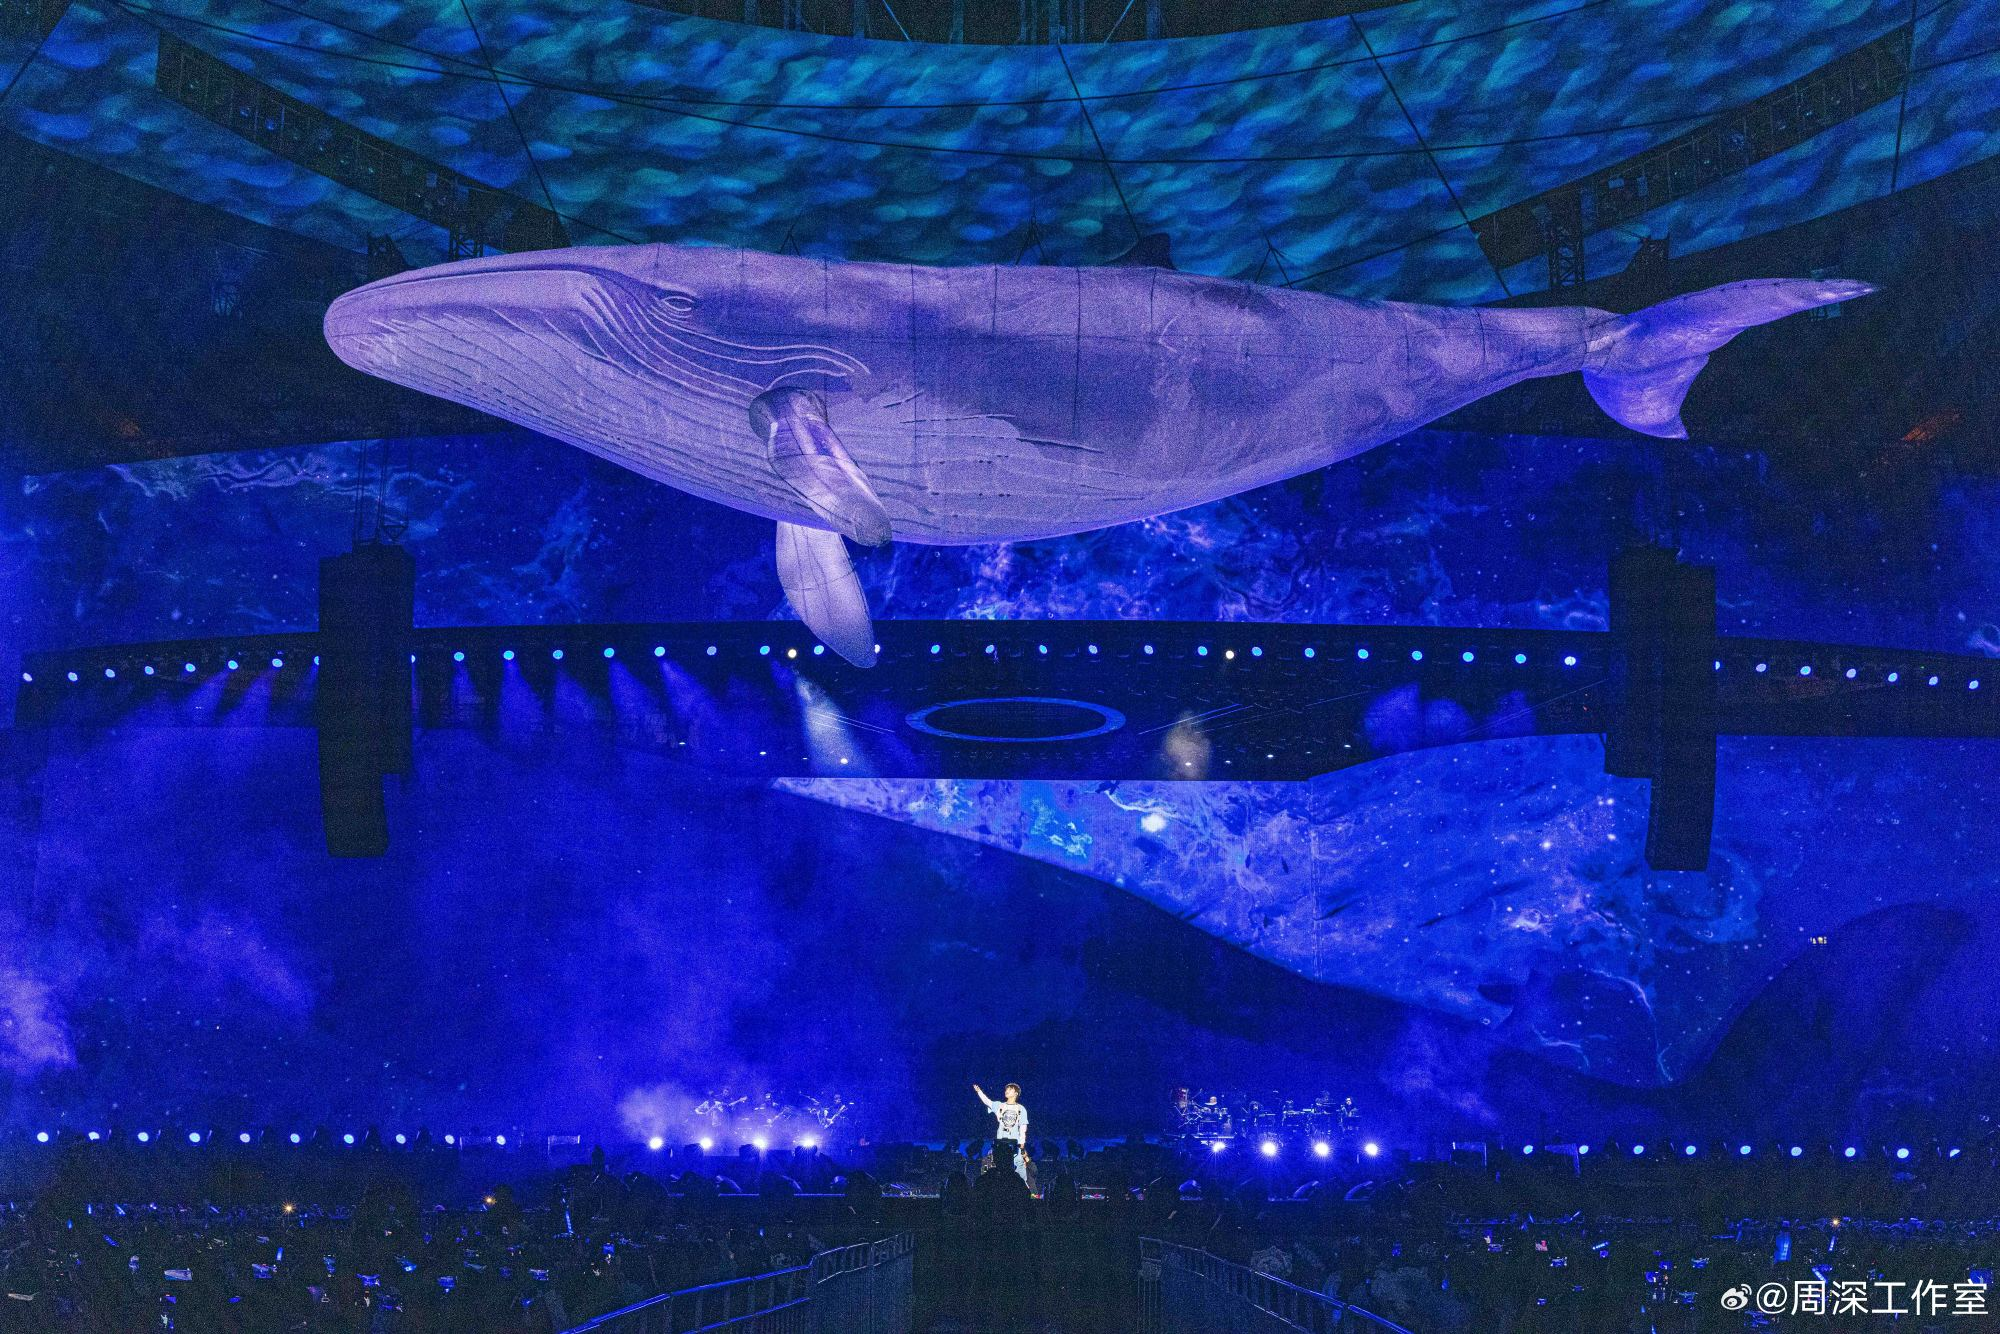
\includegraphics[width=400pt]{img/beijing20240921/big-fish} 

}

\caption{大鱼【@beijing-big-fish-day1】}\label{fig:unnamed-chunk-100}
\end{figure}

  然后呢?还想再耽误大家一点时间,还想再唱一首反深代词里面的歌,好吗?不好的话我就求求你们了,求求你们了,这首歌叫做少管我,但是说我们有一个就是少管我的特别的手势,叫做,嘿,少管我,少管我。这首歌这三个字大家初看起来会觉得有一点好像要争执,或者是不太开心的一个状态。但其实不是,少管我,就像少管我这首歌一样,它是非常轻松活泼的一首歌,它也是在提醒我们要好好的为自己负责,我们要去往更好的远方,去寻找那个自己更喜欢的自己。在这个道路当中,在不打扰别人的前提下,如果别人来打扰你的话,你就轻松乐观的说一句,嘿,少管我就好了,因为做你自己这件事,没有人比你们做得更好。还是一样的,等一下我们用相机捕捉到的人,用最大的声音让我们鸟巢近6万人都要听到你喊的少管我,好吗?喊完所有的不开心都会离你远去。

  全场倒数五个数字,5(米:4321)停,哎呀,磕到我的牙,停,你在哪里?您好,您怎么称呼?你叫天天?珍珍?珍珍你好?她叫天天,你叫天真?深深?你叫?试一下哪个队比就yeah。深深,天天,芊芊,轩轩,晚安,朋友们。等一下,全场安静,你要用最大的声音,你叫什么?轩轩?全世界是只有我没有听清,她叫什么名字?真天,等一下,一个人说,戴帽子的,甜甜,等一下,萱萱,娟娟,娟娟,我的麦克就在这里了,晚安,等一下,我要求助下,他叫娟娟,欢迎娟娟,可以冒昧的问一下,您多大吗?几岁啊。好的,61岁?我们现场有没有6岁的小朋友?有哦,那里有跟您同龄的人哟。哈哈哈,您听我的歌什么时候啦?多久了?您是来自哪里的朋友,哦,又是我们台湾的朋友,你好,呼呼,那你要用最大的声音让大家听到哦,嘿,少管我,学会没有,但是要小心前面朋友的脑袋,不要打到。哈哈哈,你要让我们全场定6万的人听到哦,不过刚才我都没有听到她的名字,你是最棒的,娟娟?是娟娟吧?芊圈?天圈?芊芊?(清唱了一句千千阙歌),你那里是圈圈出,喊出你,来,全场最大声音,321,让你们喊嘿少管我啦。千圈,圈圈,千千,天天,真真,少管我喊你什么名字来,哈哈哈。喊出这四个字,321。所以是芊芊,对不对?芊娟,哈哈哈,全场恭喜我,我终于知道她叫什么名字了,芊娟,我喊你的名字你敢答应我吗?哈哈哈,来喽,321,好,谢谢你。

  我们全场再次倒数五个数字,543,喵呼,哈哈哈,感觉是一位很难配合我的朋友,哈哈哈,您在哪里?哇,你好,我们今天最大的难题,你叫什么名字?哈哈哈,你不是应该对着我喊吗?不行,我要用我的肉耳,哈哈哈。32,好,大家保持安静啊,321。你叫什么名字?等一下,你为什么也叫娟娟?你也叫芊娟,芊芊真真?君君?你叫君君,你们耳朵好好啊。君君是来自哪里?哦,我可以不用那么大声,君君是来自哪里的朋友,为什么全场都听见了,就只有我没听见?是来自北京的朋友,北京的君君,你听我唱歌多久了?从贝加尔湖畔的时候?那你是看着我出道的诶,那你起码有10岁了,对不对?哈哈哈,小朋友笑什么,你起码是没有到10岁。好了,来,用最大的声音喊,喊开所有的不开心,321,哇,这个声音很棒,我们全场将近6万的朋友跟我一起321,嘿,少管我,\textbf{你们太棒了,所有的烦恼一定会离你们远去的\textasciitilde{}}

\begin{figure}

{\centering \includegraphics[width=400pt]{img/beijing20240921/002} 

}

\caption{原来你生来就属于天际}\label{fig:unnamed-chunk-101}
\end{figure}

\hyperref[watch-ur-manners]{🎵【\textbf{少管我}】}芊芊娟娟芊娟,所有人都要开心好吗\textasciitilde 全场\textasciitilde54321\textasciitilde 全场\textasciitilde54321\textasciitilde 你们好吗\textasciitilde{}\textbf{你们是全世界最棒的},谢谢你们,谢谢你们来,谢谢你们看到了我,好好照顾好自己好吗,我们一定会相遇的,在下一次相遇之前好好照顾好自己,听到了吗?谢谢你们,证件不要掉了,手机不要掉了,东西不要丢了哟\textasciitilde 谢谢,看台的朋友\textasciitilde54321\textasciitilde 你们太棒啦\textasciitilde 注意安全,东西不要掉了,54321\textasciitilde 最后一次,54321\textasciitilde 谢谢你们,好好照顾好自己,\textbf{\textcolor{red}{我爱你们~} }

\chapter{2024.09.22北京场}\label{beijing-20240922}

\begin{quote}
\textbf{\emph{我真的很希望一生和你相依。------ 周深}}
\end{quote}

\begin{figure}

{\centering \includegraphics[width=320pt]{img/playlists/playlists-beijing-20240922} 

}

\caption{2024周深9.29Hz巡回演唱会2024.09.22北京第二场歌单}\label{fig:unnamed-chunk-103}
\end{figure}

\newpage

\section{Part1}\label{beijing-20240922-part1}

\hyperref[opening-vcr]{🎥【\textbf{开场VCR}】}

\hyperref[I-will-go-my-way]{🎵【\textbf{借过一下}】}北京的朋友们,你们好吗\textasciitilde{}

\hyperref[Monsters]{🎵【\textbf{Monsters}】}

\hyperref[hua-shen-gu-dao-de-jing]{🎵【\textbf{化身孤岛的鲸}】}北京的朋友们,你们好吗?(米:好)愿意跟我一起唱吗?(米:愿意)到你们喽\textasciitilde 看台的朋友,大声点\textasciitilde 到你们\textasciitilde 看台的朋友\textasciitilde(深:我想给你能奔跑的岸头)(米:没有墙头)你们猜我信不信?看台的朋友猜我信不信(\textbf{深:无论你们有多少个墙头,你们依然是国王和王后})。

  北京的朋友,你们好吗?(米:好)大家好,我是歌手周深,我们又在鸟巢相见啦,谢谢大家来到9.29Hz巡回演唱会,演唱会为什么叫做9.29Hz呢?是因为人类可以听到的声音是20Hz到20000Hz之间。然后,我自己认为我是一个比较没有那么容易被接受或者是被喜欢的歌手,所以我觉得自己是一个很渺小的歌手,甚至很有可能没有办法被听见。但是\textbf{全世界最善良、最美好、最具有善意的你们听到了我,所以我们在这里相聚了,谢谢每一个生米,谢谢每一个听到我的人。}谢谢你们让我不害怕黑暗,因为我发现哪怕我一个人走在暗巷的时候,你们依然是我的光亮。也希望歌手周深加油,能够成为你们的光亮,好吗?(米:好)大家掌声欢迎钱雷老师。

\hyperref[silver-linings]{🎵【\textbf{光亮}】}你们好吗\textasciitilde【深深逗雷哥】(深:最无畏的你)(雷哥起身)(深:光亮你自己)谢谢雷哥(雷哥起身准备下班)(深:最无畏的你\textasciitilde)掌声感谢雷哥(雷哥再次准备下班)(光亮你自己)

\hyperref[ruomeng]{🎵【\textbf{若梦}】}\textbf{每次遇见你们都像是一场梦一样\textasciitilde{}}(深深戏精表演弹琴)等一下用最大的声音跟我一起合唱哦,你们(唱的)是最好听的版本\textasciitilde 到你们喽,(米:往事流转,在你眼眸)大声一点,看台的朋友\textasciitilde{}\textbf{你们太棒啦\textasciitilde{}}大声\textasciitilde(米:往事流转,在你眼眸)看台的朋友\textasciitilde 全场最大声\textasciitilde(\textbf{深:唯愿你你你你\ldots.你你你能得到拯救})

\hyperref[floating-light]{🎵【\textbf{浮光}】}跟我一起\textasciitilde{}\textbf{在这人世间恍惚三万天当中,遇见你就是最美的浮光\textasciitilde{}}

\section{Part2}\label{beijing-20240922-part2}

\hyperref[senself-vcr]{🎥【\textbf{反深代词VCR}】}

\hyperref[brave-heart]{🎵【\textbf{请我不改}】}全场嗨起来\textasciitilde 看台的朋友\textasciitilde{}

  大家好,我还是周深。你们对这样的风格的周深感觉到陌生吗?不陌生。那你不会是听了周深的新专辑反深代词吧?谢谢谢谢,谢谢我的生米们,然后也介绍一下我自己的新专辑叫做反深代词,刚才那首歌就是反深代词里面的歌叫请我不改,他说的是因为最近几年有个词很有热度,叫做PUA,就很多时候你会发现,诶,好像自己一直处在一个非常低气压的状态,但是好像大家会忘记的另外一种状态就是不停的自我苛责,自我否定,就是一种自我PUA的状态,所以就像刚才请我不改写的一样。当你发现诶,好像你的生活当中无法喘息的时候,你发现追兵与逃兵居然都是你自己,所以希望你可以认清自己,爱自己,做自己,有的时候也要放过自己好不好?那我们来看一下反深代词当中还有什么样的周深吧\textasciitilde{}

\begin{figure}

{\centering \includegraphics[width=400pt]{img/beijing20240922/002} 

}

\caption{请我不改 【@weibo-charlie-studio】}\label{fig:unnamed-chunk-104}
\end{figure}

\hyperref[mirage]{🎵【\textbf{蜃楼}】}

\hyperref[the-giver]{🎵【\textbf{警报}】} 谢谢大家,谢谢,谢谢\textasciitilde{}

  大家好,我是歌手周深,你们好吗?看台的朋友你们好吗?(好)刚才演唱的三首歌都是新专辑反深代词里面的歌曲,希望大家可以去听一下这张新专辑,如果不愿意的话,求求你们了,大家去听一下这张专辑。里面一共是我的十二个化身,果然我们南方人的前后鼻音比较难分,12个化身会在200年后,刚才的第一首歌是请我不改,就是希望自己放过自己,然后刚才第二首叫做蜃楼,他是由执念组成的一个蜃楼,有的人被困在蜃楼当中,他觉得很痛苦,但有的人被困在比较好的执念当中,他就会变得越来越好。但无论怎么样都不是错,所以这个世界上没有就是要么就是对,要么就是错的这样的答案。然后刚才那首叫做警报,是送给每一个,就是想要照顾所有的人,想要照顾每一个朋友、每个环境存在的每一个人,哪怕是陌生人的人,但是最后却偏偏忘记照顾好自己的那个人,所以希望如果你是这样人的话,可以听到刚才的那一首警报,然后开始好好爱自己好吗?其实我也有就有看到,就说周深在演唱会是不是没有话说了,就是不停的在反复让大家一定要好好的爱自己,好好照顾好自己。我后面也想了一下,其实不是,因为我认为我们能够相遇在这里,我们一定多多少少有一些部分是比较相似的,而我其实,我认为我是一个不太那么会好好爱自己的人,而\textbf{在我自己经历过那么多年的成长,包括出道十周年之后,我会发现所有的苦痛都不及,那个就是自己没有好好照顾好自己带来的那个苦痛更痛。}所以我觉得\textbf{只要你开始好好爱自己,所有的美好都会慢慢慢慢向你奔跑而来,}好吗?(米:好)有没有人觉得自己好像有一部分跟我很相似的?(米:有)我好像没有听到看台朋友们的声音,有吗?我也很开心,在很多的综艺舞台上也有不一样的周深,那么这首歌是长什么样子的呢?

\hyperref[haven-song]{🎵【\textbf{天堂岛之歌}】}谢谢大家\textasciitilde{}

  有没有是通过刚才那首歌认识我的呀?如果没有的话,你们刚才听完那首歌之后会感到害怕吗?(米:不会)大家胆子挺大的。前面,告诉他一个小秘密,就前面那一段,(一个、两个、三个小朋友)也是,我自己就是躲在被窝里,然后自己录的那一段。好,那接下来这首歌我是需要你们跟我一起大声合唱,你们准备好了吗?它可以说是我们9.29Hz巡回演唱会里面的一道考题。它是一个童话故事,他的主人翁的名字非常难念,我们随机考一下,看台的朋友,他的主人翁叫达拉,(米:达拉崩吧斑得贝迪卜多比鲁翁)离我近一点的朋友,题目就比较难了,你们,昨天我考的时候公主的名字没有难倒,请问他们回到的那个城市叫做?我还不信,我还考不到你们,那个城市的名字我都记不得。那等一下跟我一起大声唱这首达拉崩吧好吗?(米:好)

\hyperref[dalabengba]{🎵【\textbf{达拉崩吧}】}大家嗨起来,看台的朋友\textasciitilde 现在你们准备好了吗?现在到你们的时候了哟,想想他的名字叫什么,拯救了谁呢?于是\textasciitilde(米:达拉崩吧斑得贝迪卜多比鲁翁)砍向\textasciitilde 然后\textasciitilde 咬了\textasciitilde 大声点,最后\textasciitilde 看台的朋友\textasciitilde 再来一遍哦,他的名字叫达拉(米:达拉崩吧斑得贝迪卜多比鲁翁)砍向昆图(米:昆图库塔卡提考特苏瓦西拉松)这么爱念(深:要念你来念吧\textasciitilde)谢谢你们\textasciitilde{}

  好像听说在演唱会当中指向哪里,哪里就会有欢呼声,是这样的吗?真的是这样的吗?我不相信诶,那如果是指向看台也会有声音吗?那如果是那边的看台呢,我们今天有近6万的观众,那如果我是这样的话呢,那我想听一下近6万的观众在鸟巢喊钱雷的名字是什么样的?321,(米:钱雷)感觉像钱磊老师欠了大家什么。哈哈哈,我觉得就\textbf{大家都会夸我很有仪式感},我觉得钱磊老师也是最有仪式感的人,毕竟来了鸟巢,头上还顶了一个鸟巢来了,哈哈哈,给大家打个招呼吧。(钱雷:大家好)雷哥,他的名字大家可能比较陌生,他的样子大家可能更陌生,但他的作品大家很熟悉,来唱一两首吧。(钱雷:怕你飞远去,哈哈哈)(深:祝你踏过千重浪,能留在)(米:能留在爱人的身旁)停,不能唱太多,哈哈哈,很多很多,(深:而我将爱你所爱的)(米:爱你所爱的人间,愿你所愿的笑颜)停,好,谢谢大家的合作。哈哈哈来,你来到鸟巢了,你总要给大家正儿八经多说一点,不要说自己内向,我也很内向。(钱雷:呃,我觉得,鸟巢一定要来,因为)是第几次来到鸟巢?(钱雷:第一次吧)我也是一次在鸟巢开演唱会,所以要谢谢每一个到来的你们,一句话,你此时此刻最想说什么?(钱雷想说但被调皮的深深抢走话筒)谢谢,那接下来这首歌希望大家喜欢,我经常说雷哥写歌太难了,你是人吗?就现在就故意这样做的,这首歌叫做人是\_哈哈哈\textasciitilde{}

\hyperref[renshi]{🎵【\textbf{人是\_}】}没弹好,重来,重来一遍吧,来,321,哈哈哈,好好,我错了我错了我错了,好好唱歌,人是\_,希望大家喜欢\textasciitilde 一起\textasciitilde(弹指间湮没我\textasciitilde)掌声送给雷哥\textasciitilde{}\textbf{\textcolor{red}{我爱你们~} }

\section{Part3}\label{beijing-20240922-part3}

  鸟巢的朋友们你们好,大家有找到我在哪里吗?话说我第一次来到北京的印象就是,我发现,虽然网上有个梗,都说,哈哈,北京人都是鲨鱼,有人知道这个梗吗?但是在我心中我觉得北京人每个人都是指南针,我第一次来到北京,然后就北京人特别的热情,就是你去求助的话,他们都会非常热心地帮助你。我就说,诶,请问一下先生这里怎么走?然后他说这个地方很近,你前面走10米,向西转,然后再走10米再向东走,我在想哪里是西啊?然后,然后就那个时候也没有手机,然后手机也没有定位什么的,就完全都不会。然后我妈妈的手机它也没有定位,我们就不知道该怎么走,然后我们就又问了个朋友,他说,噢,很好走,你前面就往西走了10米之后再往东转,然后干嘛?哪里是西啊?直到现在我到北京我都不敢问路,因为我真的不知道哪里是西边,哪里是东边,因为我们就是真的没有这个,为什么大家不用左右呢?所以也会有北京朋友有这样的困扰吗?我听到了非常大的声音说没有,好的,我输了,对不起。接下来这首歌非常的温暖,现在天气越来越凉了,大家一定要记得多添加衣服好不好?大家有穿够衣服吗?比如我,像我一样加了秋衣?接下来两首歌也是非常非常温暖的两首歌,它温暖的就像秋衣一样,哈哈哈,希望你们喜欢。然后你们听完我弹奏钢琴之后就会发现,哇,刚才到底是哪里来的信心去说钱雷弹的钢琴弹得不好,哈哈哈,总之希望你们喜欢\textasciitilde{}

\hyperref[my-only]{🎵【\textbf{My Only}】} \hyperref[rubia]{🎵【\textbf{Rubia}】}\textbf{\textcolor{red}{我爱你们~} } 谢谢你们\textasciitilde{}

\hyperref[happy-ending]{🎵【\textbf{小美满}】}大家跟我一起大声唱好吗?(米:好)你们(唱的)是最好听的版本哦\textasciitilde 看台的朋友,大声点哦\textasciitilde 全场\textasciitilde 你们唱得太好听啦,再大声一点哦\textasciitilde 大声点\textasciitilde 到你们了,大声点\textasciitilde 大声点\textasciitilde 谢谢你们\textasciitilde 每一次一听小美满我都觉得特别的幸福,我感觉所有的愿望都会实现的,那不如我们就在这首歌当中许一个愿望,就像我这样闭上眼睛,然后默默想好心中的愿望,然后321,愿望就会挂在这棵许愿树上,所以现在在现场的你,无论什么年龄,无论什么职业,就在此刻闭上眼睛,我们默默地许一个愿望吧,闭上眼睛,闭上眼睛,许愿啦,听话,想想心中的愿望,我们有一个要求,就是只能够许关于自己的愿望哦。想一想有多久没有好好的问候一下自己了,多久没有好好关心自己啦,抱一抱自己吧。321,睁开眼睛哇,你们的愿望都会被听见的,都会实现的,继续加油好吗?(米:)\textbf{你们是最美好的存在\textasciitilde{}}到你们\textasciitilde 你们实在是太美好了\textasciitilde{}

\hyperref[live-happy-life-happy]{🎵【\textbf{好好生活就是美好生活}】}(深:新的一天我们一定)(米:好好)好好爱自己,是一切美好的开始,记住好吗\textasciitilde{}

\hyperref[no-worries]{🎵【\textbf{花开忘忧}】}(米:你好啊)你好啊\textasciitilde{}\textbf{北京的朋友,我们来你们家玩喽,来看你们啦\textasciitilde{}}全场跟我一起好吗\textasciitilde 大声点\textasciitilde 我们的思念,那些离开的人一定听得见,对不对\textasciitilde(米:对)我以前以为我一个人声音太小了,他肯定听不见,但是因为遇到你们,他们一定听得见,对不对?(米:对)花开忘忧,愿你无忧,花开忘忧,(米:愿你无忧)谢谢你们\textasciitilde{}

  我非常感谢你们,其实我是一个比较没有安全感的人,所以一开始也会比较害怕在大家面前展现太多面的我。(深深换衣服,米尖叫)不用惊叫,我有秋衣。\textbf{但是因为遇到你们之后,我就愿意去袒露更多的心声,就像刚才弹钢琴一样,我知道我一定弹得非常的不完美,甚至很有可能比很多小朋友弹得都不好。但是我想告诉你们的是,只要你想学一个技能,从任何时候开始都是可以的,因为永远有那样一个温暖的爱,它会接纳你每一个碎片,哪怕它是不完美的碎片,好吗?(米:好)因为我一定会接起你的每一个碎片,谢谢你们\textasciitilde{}}

  我第一次听到什么叫做唱歌,就是听到了邓丽君女士的歌声,所以我也希望自己可以成为像她这样的歌手。她的每首歌当中有很多人的记忆胶囊,就感觉里面存放了很多故事在里面。小朋友你肯定没有听过这些歌,但是你可以听一下,就是,嗯,爸爸辈、妈妈辈,或者是爷爷奶奶辈,他们听的歌声会是怎么样的感觉呢?有人会唱这些歌吗?那等一下跟我一起唱好吗?(米:好)

🎵【\textbf{邓丽君组曲}】(米:宝贝)宝你个头
\hyperref[thousands-of-words]{🎵【\textbf{千言万语}】}(深:那天起,你对我说,永远的爱着我)骗子(深:千言和万语,随浮云掠过)受伤了\textasciitilde{}
\hyperref[on-the-water-side]{🎵【\textbf{在水一方}】}大家跟我一起唱好吗\textasciitilde 全场\textasciitilde{}
\hyperref[only-with-me]{🎵【\textbf{路边的野花不要采}】}墙头很多的人,可给我听好了,你们说(深:路边的野花)怎么样(米:你不要采)记住了啊\textasciitilde 你们会忘记我吗?(米:不会)\textbf{我只在乎你你你你你}
\hyperref[only-you]{🎵【\textbf{我只在乎你}】}大声点\textasciitilde 看台的朋友,大声点\textasciitilde 请记住歌手周深好吗\textasciitilde(米:好)

\section{Part4}\label{beijing-20240922-part4}

\hyperref[thank-you-vcr]{🎥【\textbf{谢谢北京,谢谢你VCR}】}

\begin{figure}

{\centering \includegraphics[width=400pt]{img/beijing20240921/thank-beijing} 

}

\caption{谢谢北京!谢谢你!}\label{fig:unnamed-chunk-105}
\end{figure}

  谢谢你,谢谢北京,谢谢每一个听到我给我善意的你,谢谢你,谢谢你们看到了我。大家08年的时候在干什么呀?好的,我没有听清楚,但是我印象很深的是08年的时候,我们每个人肯定都在期待着看奥运会的开幕式,我是在贵阳的我们一个广场上的一个公众,公共大屏上一起看的,跟很多朋友们和小学同学们,哎呀,小学同学们。然后当时我就觉得,哎呀,我要是能够在北京欢迎你这首歌当中唱一句,我都觉得可是太幸福的事了。但是那个时候的我依然还是那个写不出以我的梦想为题目的作文的那个周深,因为他不知道要成为一个什么样的人。但是每天那个周深还是好好的去做好每一件事情,向前去行进着,向前去追逐着,突然就到了16年之后,周深站在了鸟巢跟大家相遇了,所以我特别兴奋能够在鸟巢跟大家一起唱起这首歌,北京欢迎你,你们愿意跟我一起唱吗?(米:愿意)

\hyperref[welcome-to-beijing]{🎵【\textbf{北京欢迎你}】}大声点\textasciitilde 全场\textasciitilde 大声点\textasciitilde 谢谢你们,而且我们今天的音响总监也是当年奥运会开幕式的音响师金少刚,我们继续向前冲,有勇气就会有奇迹,好不好?(米:好)大声点\textasciitilde 看台的朋友\textasciitilde 再大声点\textasciitilde(北京欢迎你\textasciitilde)

\begin{figure}

{\centering \includegraphics[width=400pt]{img/beijing20240922/001} 

}

\caption{北京欢迎你 【@weibo-charlie-studio】}\label{fig:unnamed-chunk-106}
\end{figure}

\hyperref[China-in-the-light]{🎵【\textbf{灯火里的中国}】}然后就有一天,这个普通的男孩第一次登上了春晚\textasciitilde 全场一起\textasciitilde(灯火里的中国,青春婀娜\textasciitilde)一起\textasciitilde 谢谢大家\textasciitilde{}
你们能够让一个非常普通的男孩子慢慢地去靠近他的梦想,是你们创造出来的奇迹,要相信自己好不好?(米:好)再次掌声给我们的金少刚老师,鸟巢我们来了,也希望我们可以创造更多奇迹时刻\textasciitilde{}

\hyperref[magic-moment]{🎵【\textbf{奇迹时刻}】}\textbf{大家嗨起来\textasciitilde{}}看台的朋友\textasciitilde 大家好\textasciitilde【魔术时间】\textbf{小小魔术师又来了哟,}大家掌声再次有请雷哥\textasciitilde 而且还有哦,321\textasciitilde 谢谢大家\textasciitilde{}
每次一到魔术的段落,教我魔术的唐老师都在下面,哎呀,哈哈,但是在反深代词当中,还想再拜托大家听一下里面的歌好不好?里面有一个快乐密码,它叫做,wala li longla,没错,只要喊起这个密码,它就会给你带来无限的快乐。我们等一下试一下好不好?来试一下,wala,看台的朋友,wala li,wala li long,wala li longla,\textbf{希望快乐永远在你身边\textasciitilde{}}

\hyperref[wala-li-longla]{🎵【\textbf{wala li longla}】}全场嗨起来\textasciitilde 哎呀,我一个人的声音太小了,你们愿意跟我一起大声喊起这个快乐密码吗?看台的朋友也愿意吗?那么等一下全场跟我一起好吗?wala,wala li \ldots\ldots 大声点\textasciitilde 看台的\textasciitilde 看台的\textasciitilde 全场\textasciitilde 全场,321\textasciitilde 我还想再听一次,321\textasciitilde(米:wala li longla)你们一定是全世界最快乐的人,谢谢大家\textasciitilde{}

  那接下来这首歌非常的巧妙,在这个地方唱起来。鸟巢大家都知道是08年奥运会开幕式的地方,那这首歌在今年奥运会也被剪进了很多我们奥运健儿们的精彩瞬间,当他/她的背景音乐,我觉得我们每个人的人生也是不停地在向前冒险,向前探索,但是我们每个人一定可以收获属于我们自己的璀璨的,对不对?你们可以创造奇迹,把一个非常普通的男孩周深送到那么多那么多那么大的舞台,周深可以做到的,你们一定也可以,向前冲吧,璀璨冒险人\textasciitilde{}

\hyperref[adventurers]{🎵【\textbf{璀璨冒险人}】}跟我一起好吗(他们说要越过前方风沙必须低着头\ldots\ldots)大声点\textasciitilde 全场\textasciitilde 大声点\textasciitilde(米:还想要继续吗)要\textasciitilde 看台的\textasciitilde{}\textbf{不要害怕自己不完美,继续向前冲好不好?(米:好)}

【\textbf{点歌环节}】现在到了我们9.29Hz巡回演唱会的点歌时间啦。哇,你好漂亮,唔,你们都好漂亮啊,谢谢你们。全场帮我倒数五个数字好不好?(米:好)5(米:4321)他是,你,感觉,感觉从你的脸的表情不是很开心。哈哈哈,在这里。你好,在哪里啊?你好,怎么称呼您?(吴京润)有没有小名哦?胡京瑞?(吴)吴京瑞?(润)吴京润(对)一般怎么称呼你,都是直呼大名吗?也不是吧(京润)哈哈哈,好,京润朋友,您是来自哪里的朋友?(黑龙江)黑龙江的,哇哦,那我们全场近6万的朋友欢迎黑龙江的朋友京润,(谢谢,谢谢深深),也要谢谢大家,(谢谢大家),谢谢哪些人?(现场所有的朋友们,谢谢)现场是哪里?(鸟巢演唱会所有的朋友们,谢谢你们)谁谢谢鸟巢现场所有的朋友们,(谢谢周深!)什么时候开始听我的歌的呀?(好久好久)好久(16年),哦第六年了,谢谢你。(16年)16年的时候,很久了耶,(这是我第一次看演唱会),谢谢谢谢谢谢,现场有没有跟京润一样是第一次开演唱会的?那有没有谁是第一次来到鸟巢的?哇,这么多朋友,\textbf{谢谢你们把我带到了这么多可能的舞台,}谢谢你们。请问一下您多大呢?(29)那我们差不多是同辈的,嗯,笑这么大声是什么意思?也就是说,好吧,你上面有没有喜欢听的歌?舞台这边就是一些,就是大家从舞台上认识我的,比如像我刚出道的舞台啊,天赐的声音上面啊,或者是像蒙面唱将里面的歌,然后录音棚这边就是我自己的歌曲,然后中间是返场,是在我们9.29Hz点歌中间出现的两首歌,可它爱着这世界和随风,你会比较偏向哪边?他的眼睛已经很明确,偏向的是舞台这边。(是的)你第一次听我的歌是哪首?(欢颜)你不会是等一下,你不会是你哦。哎呦,(有可能会有反转哦)现在的朋友们越来越难聊天啦,好的好的,那来吧,你想为我们9.29Hz巡回演唱会北京站鸟巢第二场选择?(孤独的牧羊人)哇,你有很多惊喜啊,好,谢谢京润,谢谢(谢谢)谢谢你,这首歌有点压力啊,那我们就试试吧\textasciitilde{}

\begin{table}

\caption{\label{tab:unnamed-chunk-107}2024周深9.29Hz巡回演唱会09.22北京场点歌歌单}
\centering
\begin{tabular}[t]{lll}
\toprule
舞台 & 返场 & 录音棚\\
\midrule
1-欢颜 & 1-可它爱着这个世界 & 1-春雪\\
2-身骑白马 & 2-随风 & 2-荒城渡\\
3-贝加尔湖畔 &  & 3-独白\\
4-兰亭序 &  & 4-和光同尘\\
5-漂洋过海来看你 &  & 5-曾经沧海\\
\addlinespace
6-独上西楼 &  & 6-茧\\
7-只字不提 &  & 7-花开\\
8-孤独的牧羊人 &  & 8-去明天\\
9-调查中 &  & 9-愿\\
\bottomrule
\end{tabular}
\end{table}

\hyperref[lonely-shepherd]{🎵【\textbf{孤独的牧羊人}】}(深深看了眼观众,歌曲提词器太快,没跟上,哈哈哈哈)对不起,再来一下,大家就当没有发生过,好321,京润,起来陪我演一下这段,谢谢京润\textasciitilde 你们看那边\textasciitilde 哦,我这么漂亮的衣服都被呛到了\textasciitilde 哎呦,有好多小朋友哦\textasciitilde 谢谢\textasciitilde{}

  全场帮我再倒数五个数字,5,(米:4321)又是一位看起来好像不是很开心的,我们的点歌太真实了,您在哪里?噢,在那里对不对?哈喽,给大家打个招呼。(一位61岁坐轮椅来的阿姨)哦哦哦哦,对不起,对不起,哎,如果不太方便可以坐着的,没事的,我们可以坐着聊,我也可以坐着,(没事,站着吧)已经站着了。好了,那怎么称呼您?(你好,我叫龚金英)龚金央?龚金央?(对)准确的找到了我这个南方人最难发的两个音,哈哈哈,龚金英,好,应该怎么称呼您更亲切一点呢?(嗯,你叫我龚阿姨吧)龚阿姨好,(深深你好)您好,可以问一下您今年的年纪吗?(我今年61)好巧啊,因为昨天我们也有一位61的朋友,您是?您应该是来自北京当地的吧?(对)哎呦,你看我这耳朵还挺好使儿。您是什么时候开始听我唱歌的啊?(应该是在17年,18年那会儿)您听到的第一首歌是大鱼耶,谢谢谢谢。旁边这位陪您来的是(我的儿子),应该怎么称呼他呀?(他叫邵维)让他给大家打个招呼,咱们用麦克打招呼,(大家好)声音太大了,震耳欲聋了。邵维,您好,好,那您看一下您想听哪首歌呢?(漂洋过海来看你)谢谢,谢谢,谢谢您,谢谢,谢谢龚阿姨,谢谢谢谢,谢谢。好,那希望您能喜欢我唱我演唱的这首歌曲,漂洋过海来看你,也是非常感动的一首歌,因为,是不是的确有很多人也是漂洋过海来看我?我有看到,有从澳大利亚来的,谢谢谢谢谢谢。这是我在舞台上唱的一首歌曲,希望大家能够喜欢这首娃娃的漂洋过海来看你,会唱的跟我一起唱好吗?

\hyperref[across-the-ocean-to-see-you]{🎵【\textbf{漂洋过海来看你}】}一起\textasciitilde(陌生的城市啊\textasciitilde)(多盼能送君千里,直到山穷水尽)我真的很希望(一生和你相依)我还有看到从北美来的朋友,谢谢,无论你从哪里来,谢谢你来看我\textasciitilde{}

\hyperref[keep-playing]{🎵【\textbf{不想睡}】}你们好吗\textasciitilde 一起\textasciitilde(不想睡,我要陪你一整夜)谢谢你们,\textbf{你们发出的光芒,的光子会在宇宙的另外一端,很多年,很多年之后它会相遇,我们就又一次见面啦},谢谢你们\textasciitilde 全场\textasciitilde 大声点\textasciitilde 到你们\textasciitilde(lalalalalalalala)和你们相遇真的太美好了,谢谢大家,大家今天玩得开心吗?\textbf{一定要用这段记忆当做是一颗糖好好的保存起来,当你需要力量的时候,希望这一颗糖能够给你力量好不好?因为它一定是我生命当中最重要的那一份甜分,谢谢你们\textasciitilde{}}

  我们也要谢谢很多很多为我们付出,让我们很好相遇的人,好不好?(米:好)感谢场地支持,国家体育场鸟巢,我喊鸟巢,然后我们一起喊我们来了,好不好?鸟巢(米:我们来了),\textbf{你们真的是最棒的。}要感谢本次巡演的全程主办,北京时代立方文化传播有限公司。感谢演唱会制作单位必应,感谢我们的总导演周佑洋,庄惟惞,感谢我们的音响总监金少刚,谢谢,感谢我们的音乐总监龙隆老师,以及感谢我们所有的乐手老师们,以及我们的合唱老师们,谢谢大家,以及要感谢我们今天的钱雷老师,虽然我也没有什么给他说话的机会,但是我替他谢谢大家啊。感谢我们的舞蹈团队SDT ShowPro,感谢服装团队设计师劳伦斯许工作室,时装品牌windowsen,音响工程南京奥斯泰,感谢我们的调音团队乐尔工作室,大家听到我的声音还悦耳吗?谢谢我们的硬体工程北京立超舞台集团。感谢周深工作室的小伙伴们,你们喊的比我唱歌的声音还大,我吃醋了,我走了。我代表周深工作室的小伙伴们,谢谢大家,我们还会继续努力的。感谢微博,感谢微博音乐,感谢微博演出。\textbf{感谢我们最美的北京,感谢北京的公安、文化、消防、应急、奥管委等所有职能部门的大力支持,}保障我们演出的顺利进行,大家感谢他们的掌声再热烈点,以及感谢我们所有现场,所有台前幕后的工作人员,感谢我们现场的安保团队们,也要感谢我们非常辛苦的志愿者们,当然最重要的是要感谢世间最美好,每一个都充满善意的来到现场的你。因为真的金少刚老师每一次都跟我说,就是你真的要好好感谢你的观众,因为你\textbf{拥有最好的最棒的观众},谢谢你们。

  那我们来合照吧。来321,这边的朋友,321,这边的朋友,哇,还有越南的朋友,321,看台的朋友,我来了。(米:加油加油)你们会让我觉得我在为了明年的奥运会在做准备,哈哈,来321,这边的朋友,321,那边的朋友,我来啦,哎呀,好累呀,来我们拍照,休息一秒,321,这边的朋友,你们好,321,谢谢大家\textasciitilde{}

  刚才的不想睡,是卡布的晚安曲,为什么是卡布?卡布是我在,大家知道有个歌手叫周深之前,我在网上自己唱歌的名字叫卡布。那现在周深有一首他自己的晚安曲,它叫我以渺小爱你,谢谢你们看到了人群当中最渺小的我,谢谢你们\textasciitilde{}

\hyperref[loving-you-in-my-humble-way]{🎵【\textbf{我以渺小爱你}】}\textbf{我不知道自己还能唱多久,我也不知道你听过我多少首歌,但是无论你是不是生米,你只要听到我,你就给了我非常大的善意,很荣幸可以在你们的人生当中出现,哪怕只有10秒副歌的时间,我很渺小,我的力量也没有那么大,谢谢你们看到了渺小的我,也谢谢你们给我不朽的爱(我以渺小爱你,同行的旅程,我以短暂爱你,不朽的旅程)谢谢你们\textasciitilde 好好照顾好自己\textasciitilde{}}

\section{Part5}\label{beijing-20240922-part5}

\hyperref[the-wind-rises]{🎵【\textbf{起风了}】}\textbf{谢谢你们来,谢谢你们还在\textasciitilde{}}以爱之名,你还愿意吗?(米:愿意)\textbf{我真的好幸福啊\textasciitilde{}}你们也一定要幸福好吗?

\hyperref[big-fish]{🎵【\textbf{大鱼}】}

\begin{figure}

{\centering \includegraphics[width=400pt]{img/beijing20240922/big-fish} 

}

\caption{大鱼【@beijing-big-fish-day2】}\label{fig:unnamed-chunk-108}
\end{figure}

  谢谢大家,我每次唱到这里,我心中只有四个字,就每次跟你们的见面我都觉得自己何德何能,谢谢你们\textasciitilde 我们一起有当年的奥运会开幕式的音响师金少刚老师,然后吊这条鱼的团队,也是当年开幕式的威亚团队,大家掌声送给老师们,也要谢谢我们所有为我们创造这一场非常幸福的聚会的老师们,大家掌声再热烈一点,朋友们,这是鸟巢啊,谢谢大家,那我还想再耽误大家一点点时间,还有一首歌是反深代词里面的歌叫少管我,它听起来也许有一点点争议,他感觉像吵架,但是想要告诉大家,像这首歌一样要轻松活泼,我们要对自己负责,我们要知道怎样去成为更好的自己,因为我们的梦想一定会实现,不要害怕中间任何的一些挫败或者失败,好吗?当在不打扰别人的前提下,如果别人来影响你的节奏,我们就轻松说一句,嘿,少管我好吗?我们还是会用相机捕捉两位朋友,然后让他喊出最大的声音,全场倒数五个数,5(米:4321)停,您好,来到了最难的这个环节,你叫什么名字?何伊,Joey,oh,Joey,欢迎Joey,你是来自哪里的朋友?上海,好的,用你最大的声音,让我们全场近6万的人能听到你的嘿,少管我,321,谢谢你\textasciitilde 全场的朋友,我想听到你们跟我一起,嘿,少管我好吗,321,(米:嘿,少管我)所有的不开心都会离你而去的\textasciitilde{}

\hyperref[watch-ur-manners]{🎵【\textbf{少管我}】}谢谢你们,我忘了说一句话,\textbf{\textcolor{red}{我爱你们~}}全场\textasciitilde321\textasciitilde 全场,54321\textasciitilde 看台的朋友,等下要大声点哦\textasciitilde54321\textasciitilde 全场\textasciitilde321\textasciitilde 全场\textasciitilde54321\textasciitilde 谢谢你们,注意安全,证件不要掉了,手机不要掉了,一定要平平安安的到家好不好?我们一定会再次相遇的,看台的朋友,谢谢你们,在我们相遇之前替我好好照顾好自己,答应我好不好?(米:好)54321,谢谢你们\textasciitilde{}

\begin{figure}

{\centering \includegraphics[width=350pt]{img/beijing20240922/003} 

}

\caption{不舍 【@weibo-charlie-studio】}\label{fig:unnamed-chunk-109}
\end{figure}

\begin{center}\rule{0.5\linewidth}{0.5pt}\end{center}

\begin{figure}

{\centering \includegraphics{img/weibo/beijing-20240923} 

}

\caption{周深国家体育场(鸟巢)演唱会结束微博 【@weibo-charlie】}\label{fig:unnamed-chunk-110}
\end{figure}

\chapter{2024.10.06重庆场}\label{chongqing-20241006}

\begin{quote}
\textbf{\emph{同频的人是一份礼物,你们是我今生最大的礼物。------ 周深}}
\end{quote}

\begin{figure}

{\centering \includegraphics[width=320pt]{img/playlists/playlists-chongqing-20241006} 

}

\caption{2024周深9.29Hz巡回演唱会2024.10.06重庆第一场歌单}\label{fig:unnamed-chunk-113}
\end{figure}

\newpage

\section{Part1}\label{chongqing-20241006-part1}

\hyperref[opening-vcr]{🎥【\textbf{开场VCR}】}

\hyperref[I-will-go-my-way]{🎵【\textbf{借过一下}】}重庆的朋友们,你们好吗?

\hyperref[Monsters]{🎵【\textbf{Monsters}】}

\hyperref[hua-shen-gu-dao-de-jing]{🎵【\textbf{化身孤岛的鲸}】}大家好,我想要你们跟我一起合唱这首歌,好吗?(米:好)到你们\textasciitilde 大声点\textasciitilde 看台的朋友\textasciitilde 到你们\textasciitilde 看台的朋友\textasciitilde{}
(深:我想给你能奔跑的岸头)(米:没有墙头)我科普一下,就是现在他们在喊的是没有墙头,但是你们猜我会信吗?(米:会)我才不信,看台的朋友们信吗?(\textbf{深:但是无论如何,你们都是自己的国王和王后})谢谢大家\textasciitilde{}

  重庆的朋友们,你们好不好?\textbf{你们太热情了,好开心},但是没有想到重庆冷的我穿了秋衣,刚才其实非常投入的在唱 monsters,那个pose,I see your monsters,然后一看就是\textbf{I see your 秋衣,I see your 没有穿秋裤了,今天。}欢迎大家来到9.29Hz巡回演唱会重庆站,你们好吗?谢谢你们,\textbf{因为人耳可以听到的频率是20到20000Hz,我一直觉得自己也是一个比较难容易被接受的歌手,就像9.29Hz这样的频率一样没有办法被听到,但是因为你们,我被听到了,谢谢你们。也非常非常感谢你们选择听歌手周深的歌,谢谢你们看到了我,你们好吗?}(米:好)说实话,我以前一直以为有了导航之后我再也不会迷路了,直到我来到了重庆,开了一个导航点,可能它还分几层,哈哈哈,但是\textbf{我觉得我不害怕,因为无论我看向任何地方都可以看到光亮。谢谢你们让我不孤单,请相信只要你们需要,我就在这里},好吗?(米:好)看台的朋友,你们好吗?

\hyperref[silver-linings]{🎵【\textbf{光亮}】}\textbf{我觉得你们嗓子都比我的嗓子好,你们是来踢馆的吧}\textasciitilde(深:光亮你自己)谢谢你们\textasciitilde 摇起你们的荧光棒\textasciitilde(深:最无畏的你\textasciitilde)也请记得现在天冷了(深唱:记得穿秋衣)\textasciitilde{}

\hyperref[ruomeng]{🎵【\textbf{若梦}】}(捣蛋鬼模仿弹古筝)没了?\textbf{遇见你们就像做了一场梦一样,这个梦是真实的吗}?(米:是)\textbf{那等下让我听到最好听的版本好不好?(米:好)}谢谢\textasciitilde 到你们喽,(米:往事流转,在你眼眸)太好听了,再来\textasciitilde 太好听啦\textasciitilde 大声点(米:往事流转,在你眼眸)看台的朋友(米:一边遗忘一边拼凑)全场最大声\textasciitilde(深:因为你们,我才得到拯救,希望你能)(米:得到拯救)谢谢大家,\textbf{你们唱的太好听了,我都在觉得你们是来踢馆了吗?但是真的非常开心,在这人生恍惚三万天当中,我们相遇啦,谢谢你们愿意和我同频,同频的人是一份礼物,你们是我今生最大的礼物\textasciitilde{}}

\hyperref[floating-light]{🎵【\textbf{浮光}】}一起\textasciitilde(深:浮光掠影\textasciitilde)

\section{Part2}\label{chongqing-20241006-part2}

\hyperref[senself-vcr]{🎥【\textbf{反深代词VCR}】}

\hyperref[brave-heart]{🎵【\textbf{请我不改}】}嗨起来\textasciitilde 嗨起来\textasciitilde(深:请我不改\textasciitilde)

  大家听得还开心吗?(米:开心)雨衣带一下,好像有点飘雨了,啊啊啊,不要再下雨了。但是有没有人觉得,诶,好像在演唱会里看到了一个不一样的周深?看台的朋友有没有看到不一样的周深耶?谢谢大家,刚才是我的新专辑(米:反深代词)对,谢谢,我发新专辑了,反深代词里面的歌,然后像刚才请我不改这样的不一样的周深,在这张专辑里还有11个,希望大家去听一下好不好?如果不愿意的话就是我求求你了,去听一下,谢谢,\textbf{刚才请我不改这首歌是非常嗨,非常硬核的,因为很多时候我们会觉得,有个熟悉的词叫PUA,我们会觉得很多时候就是被周围环境PUA,但是大家忘记了一种就是自我PUA,很多时候我们都渴望变成更好的自己,这当然是非常好的。但是很多时候我们给自己过于太大的压力,所以我们要爱自己,认识自己,做好自己的同时,偶尔也要学会放开自己,好吗?(米:好)答应我一定要好好的爱自己},好不好?(米:好)那我们来看一下反深代词当中它还有什么样的周深呢?

\hyperref[mirage]{🎵【\textbf{蜃楼}】}

\hyperref[the-giver]{🎵【\textbf{警报}】}

  重庆的朋友们,你们好吗?\textbf{非常非常感谢大家愿意在这么珍贵的假期当中来和我相遇},谢谢你们,谢谢,刚才新专里的新专辑里面的歌大家觉得好听吗?(米:好听)那有人没有说好听,那就求求你去听一下,哈哈哈哈,第一首歌是请我不改,第二首歌是蜃楼,他说的是200年后有一座所有人的执念形成了一个蜃楼,可能有好的执念,它会帮助你变得越来越好,但是可能也有不好的执念把你困在原地,好像不知道该往哪里走快,所以你们该往哪走呢?\textbf{我就不一样了,我知道我想要去到我的歌迷的心里,糟糕,演唱会越来越开,自己越油腻},但是有个美好的祝福,就是无论是好的执念还是坏的执念,都希望能够你变得越来越好,所以就来到了第二首歌,叫做\textbf{警报,这首歌是写给很多人,非常,很多非常善良的人,他们想要照顾整个环境的人,想要照顾所有人,担心今天他是不是心情不好?会担心自己会不会因为有一句话会觉得诶,得罪了他或什么之类的,但是大家担心左担心右,最后却往往忘记担心自己没有照顾好自己。所以刚才的警报声是发给这样忘记好好爱自己的人的},你们是这样的人吗?(米:不是)我听到不是,我又非常开心,但是还有很多人没有回答,所以请你随时记住这个警报声,要好好的爱自己好不好?(米:好)因为我觉得我们之所以能够同频,我觉得我们多多少少肯定有很多相似的地方,我之前就是一个比较没有安全感的人,哈哈,但是遇到了你们我开始愿意表达自己,愿意去开始更多的认识自己,然后再到做自己。所以谢谢你们给我这样认识自己和做自己的旅程,我也希望自己的歌声可以陪伴你们去找到更好的你们自己,好吗?(米:好)刚才都说有蜃楼,对吧?但是我发现如果我开车走上我们的盘龙立交的话,我可能,因为我很爱迷路,所以我可能在上面两天都出不来,哈哈哈,有没有在我们的盘龙立交上面迷过路的?有诶,有没有本地的朋友在上面迷路的?那我现在就有个愿望,\textbf{希望自己的歌声能够像盘龙立交一样,就是让你们一直流连忘返啊}。诶,那么后面又会发生什么事情呢?

\hyperref[haven-song]{🎵【\textbf{天堂岛之歌}】}大家好,我是希望用歌声让你们逃不出去的歌手周深,你们好吗?(米:好)你们听得还开心吗?(米:开心)看台的朋友们听得开心吗?那也就说9.29Hz巡回演唱会重庆第一站的朋友们听的是不是很开心?(米:开心)

  既然听得那么开心,那就要来接受一道考题了,大家嘴皮子溜不溜?喊这么大声,\textbf{你们真的很像来踢馆的},那我来试一下,有一个我演唱的舞台,它很精彩的,一个非常美好的通话故事,里面的主人翁的名字叫做,达(米:达拉崩吧斑得贝迪卜多比鲁翁)厉害了,他砍向的那条巨龙的名字叫做昆图(米:昆图库塔卡提考特苏瓦西拉松)看台的朋友,\textbf{我听到你们在那浑水摸鱼},不得行哦,看台的朋友们,单独考一下,叫达啦(米:达拉崩吧斑得贝迪卜多比鲁翁)那登一下,登一下是哪里的口音?那等一下就跟我一起来回顾一下这个童话故事吧\textasciitilde{}

\hyperref[dalabengba]{🎵【\textbf{达拉崩吧}】}摇起你们的荧光棒\textasciitilde{}\textbf{亲爱的观众朋友们},你们复习好了吗?现在可要轮到你们来说这个童话故事喽,一脸自信的样子,来一下哦\textasciitilde 于是\textasciitilde 砍向\textasciitilde 然后\textasciitilde 大声点,咬了\textasciitilde 看台的朋友\textasciitilde 最后\textasciitilde 大家再来一遍哦,他的名字叫达拉(米:达拉崩吧斑得贝迪卜多比鲁翁)打败了昆图库(米:昆图库塔卡提考特苏瓦西拉松)这么爱念(深:要念你来念吧)我们成功啦,非常感谢大家。有没有人是看像刚才的达拉崩吧的舞台听到歌手周深啊,有没有人是像看电视剧听到的歌手周深呢?(米:有)那有没有人是听到反深代词听到的周深啊(米:有)骗子,\textbf{但是我很开心,我可以通过很多很多的屏幕和通过很多很多的方式被大家听到,然后当然也很开心的是能够在电影当中被大家听到哦,看台的朋友们,你们听过我吗}?听过。那等一下你们要跟我一起唱这首歌,你们愿意跟我一起唱吗?(米:愿意)我们试一下好不好,(深:让死亡\textasciitilde)(深:让恐惧\textasciitilde)(深:来摧毁我深爱的一切)(深:弹指间\textasciitilde)(深:打不败活着)\textbf{不记词?果然我们有相同的频率,我们都不记词,那希望大家喜欢这首人是\_。}

\hyperref[renshi]{🎵【\textbf{人是\_}】}你们会忘记我吗?(米:不会)

\section{Part3}\label{chongqing-20241006-part3}

  大家好,知道我在哪里吗?(米:知道)错,\textbf{我在你们的歌单里,这是个很幸福的事情}。\textbf{那接下来这两首歌也像秋衣一样,希望可以温暖你们,好吗?(米:好)}这两首歌应该怎样都没有想到自己会被形容成秋衣,但是也想告诉大家,无论你想学习任何一个新的技能,什么时候开始都不算晚。这句话背后的意思也就是说,也就是说等一下我如果弹得不好,记得给我鼓励,你们会鼓励我吗?(米:会,加油)我感觉鼓励的声音不是很大诶,希望你们喜欢,\textbf{才弹一个前奏就鼓励我是不是有点假?}

\hyperref[my-only]{🎵【\textbf{My Only}】} \hyperref[rubia]{🎵【\textbf{Rubia}】}谢谢你们\textasciitilde{}

\hyperref[happy-ending]{🎵【\textbf{小美满}】}你们愿意跟我一起唱吗?(米:愿意)要好好照顾好自己哦(米:好)大声点\textasciitilde(米:抓在手里捏成棉花糖)(\textbf{深深表演})大声点,一起哦\textasciitilde{}\textbf{你们唱的是最好听的哦},等下也要大声点唱好吗?哎呦,磕到我的牙齿\textasciitilde 唱\textasciitilde 看台的朋友\textasciitilde 唱\textasciitilde 大声点\textasciitilde【许愿】听小美满这首歌,我就觉得特别的幸福,\textbf{我觉得它有一股力量,所有的愿望都会实现}。所以我们重庆的朋友们愿意跟我一起在这里许个愿望吗?就像我这样,闭上眼睛,许一个愿望,然后听我喊321,睁开眼睛的时候,我们的愿望就会出现在许愿树上啦,请相信这一份美好的力量,它真的非常有用,全场的朋友,现在,无论你是什么年龄段,无论你是什么工种,闭上眼睛,听话,闭上眼睛默默许下一个愿望,看台的朋友,许好愿望,想要许什么愿望呢?但是这个愿望有一个要求,只能够许关于自己的愿望,想一想是不是很久没有拥抱自己一下了呢?是不是很久没有问一下自己最近还好吗?是不是很久没有跟自己说你辛苦了,你真的很棒啊。321,\textbf{我们的愿望一定会被听到的\textasciitilde{}}(深:笑就好,哭也好,自己)(米:就是自己最好的陪伴)\textbf{(深:你们就是周深最好的陪伴)真的要答应我好好爱自己好吗?(米:好)好好爱自己是一切美满,一切美妙的开始\textasciitilde{}}

\hyperref[live-happy-life-happy]{🎵【\textbf{好好生活就是美好生活}】}(深:新的一天我们一定)一定什么啊(米:好好)千万不要忘了我们一定好好的\textasciitilde{}

\hyperref[no-worries]{🎵【\textbf{花开忘忧}】}(深:我会说)(米:你好啊)你们好\textasciitilde{}\textbf{重庆的朋友,我们来你们家看你们啦},你们愿意跟我一起把思念唱出来吗?(米:愿意)我们的思念一定会被听见的,对吗?(米:对)\textbf{花开忘忧,愿你无忧,花开忘忧,(米:愿你无忧)}好好照顾好自己,这样他们才会开心,好不好?(米:好)谢谢大家\textasciitilde{}

  我觉得我真的每次开演唱会我脑海中只有那四个字,(喇叭没声音2秒)觉得自己何德何能够从一个非常普通的男孩子去慢慢去追逐自己的梦想,去靠近自己的梦想,\textbf{是你们带我去到了非常非常多我从来都不敢想的地方,所以每一次感谢都是发自我内心的,谢谢你们听到了我,谢谢,谢谢,谢谢你们听到了我。}我希望自己也可以成为像邓丽君女士这样的歌手,她的很多歌当中都有很多人的时光胶囊,存满了他们很多很多的记忆,所以这些每一首歌都非常的有意义,你愿意跟我一起唱吗?小朋友,一看就是没有听过吧?哈哈哈,那等一下,我们让小朋友们听一下那些歌是什么样的味道吧?

🎵【\textbf{邓丽君组曲}】
\hyperref[thousands-of-words]{🎵【\textbf{千言万语}】}\textbf{(深:那天起,你对我说,永远的爱着我)(米:爱你)骗子(深:千言和万语)都是你们的谎言(深:随浮云掠过)} \hyperref[on-the-water-side]{🎵【\textbf{在水一方}】}全场跟我一起唱好不好(米:好)看台的朋友\textasciitilde 到你们\textasciitilde(米:我愿顺流而下\textasciitilde)
\hyperref[only-with-me]{🎵【\textbf{路边的野花不要采}】}这首歌送给很多,有很多墙头的人哦\textasciitilde 要说什么话一起说(米:路边的野花,不要采)\textbf{哎呦,这几万人的呼喊,也不知道听没听进去啊\textasciitilde{}}
\hyperref[only-you]{🎵【\textbf{我只在乎你}】}到你们\textasciitilde(米:人生几何,能够得到知己)全场(米:任时光匆匆逝去我只在乎你\textasciitilde)谢谢你们,希望你们不要忘记我,我是歌手周深,\textbf{\textcolor{red}{我爱你们~} }

\section{Part4}\label{chongqing-20241006-part4}

\hyperref[thank-you-vcr]{🎥【\textbf{谢谢重庆,谢谢你VCR}】}

\begin{figure}

{\centering \includegraphics[width=400pt]{img/chongqing20241006/thank-chongqing} 

}

\caption{谢谢重庆!谢谢你!}\label{fig:unnamed-chunk-114}
\end{figure}

\hyperref[China-in-the-light]{🎵【\textbf{灯火里的中国}】}大家好\textasciitilde 等下要跟我一起唱哦,怎么这首歌回答的声音那么小,跟我一起唱哦\textasciitilde{}\textbf{祝大家国庆节快乐\textasciitilde{}}跟我一起\textasciitilde{}

\hyperref[wala-li-longla]{🎵【\textbf{wala li longla}】}(深:快乐没时差,wala li longla)嗨起来\textasciitilde{}\textbf{宝你个头啊\textasciitilde{}}看台的朋友们\textasciitilde 全场愿意跟我一起念起这个快乐密码吗?(米:愿意)你们跟着我一起念,好不好?我要听到你的声音,wala,wala li,wala li long,wala li longla\textasciitilde wala,看台的朋友,wala li,wala li long,wala li longla\textasciitilde 最后一遍,wala,wala li,wala li long,wala li longla\textasciitilde 全场\textasciitilde 全场\textasciitilde 全场最大的声音,(米:wala li longla)你们是最棒的,wala li longla,谢谢你们,谢谢大家,刚才的周深是不是也有点不一样?没错,他也是新专辑反深代词当中的歌,无论怎么样,求求你们去听一下,你们觉得好听吗,谢谢谢谢。

  但是我发现昨天我们在彩排的时候,好像这两天都没有怎么看到太阳,对不对?\textbf{但是我发现只要遇到了你们,哇,心情舒畅,甚至就是阳光到,感觉自己要涂防晒},朋友们,哈哈哈。\textbf{无论在任何时候,只要想到你们的陪伴,我都觉得我看到了太阳}。所以在重庆我就特别想唱这首歌,太阳出来喜洋洋,你们会唱吗?要跟我一起唱,看台的朋友们听到了吗?

\hyperref[happy-sun]{🎵【\textbf{太阳出来喜洋洋}】}等一下要唱大声点好不好?摇起来,来喽\textasciitilde 大声点\textasciitilde 摇起荧光棒,等下要唱的更大声点\textasciitilde 哎呀,太阳到底出来不了?再来一遍\textasciitilde{}

遇到你们就是每一个奇迹时刻\textasciitilde{}

\hyperref[magic-moment]{🎵【\textbf{奇迹时刻}】}摇起你们的荧光棒\textasciitilde 看台的朋友\textasciitilde 一起\textasciitilde【魔术时间】重庆的朋友们你们好吗?又到了揭晓时刻,跟我全场倒数三个数,(米:321)你们太厉害了,这是你们的魔法,我觉得我有点唱累了,你们可不可以请我吃一个汉堡啊?全场三个数(米:321)你们请我吃的特别好吃\textasciitilde{}

  哎呀,(彩带缠在身上)\textbf{谁牵绊了我,谁牵绊了我?原来是我的生米牵绊着我},当然非常感谢生米的同时,也非常感谢所有向我投向善意的每一个听过我的你,谢谢你们。小朋友们,刚才是一个错误示范,边运动的时候不要吃东西,你会发现,咳咳?我可以喝一口水吗?(米:可以,宝贝)宝你个头。很多时候你们说的最多的一句话就是谢谢我给你们的光,但其实是你们,每一次你们发出的光照在我的身上,是我谢谢你们让我带我去到了很多我从来没有敢想象的地方,比如像体育馆,或者像体育场,或者甚至我们之前还去过的鸟巢,对不对?(米:对)所以要相信你们自己,你们不要小瞧自己,你们的力量比我们想象中要大得多,我们每一个璀璨冒险人们,向前冲把\textasciitilde{}

\hyperref[adventurers]{🎵【\textbf{璀璨冒险人}】}给我力量好吗?(米:好)记得也给自己力量好吗?(米:好)全场跟我一起\textasciitilde 看台\textasciitilde{}\textbf{\textcolor{red}{我爱你们~} } 全场\textasciitilde 你们\textasciitilde 最亲爱的你们,(深:去追吧)谢谢你们,你们听得还开心吗?(米:开心)再一次非常感谢大家愿意把这么宝贵的假期时间和我相见,谢谢你们,再一次祝大家国庆节快乐,也要记得天天快乐好不好?(米:好)

🎵【\textbf{点歌环节}】接下来到我们的点歌时间了,请出歌单,哎呦,我还以为自己裤子破了,吓我一跳。全场倒数五个数字,我们一起找到他,歌曲分别分为三个部分,一个是舞台部分,就是大家可能在一些综艺、音综上面听到的周深,还有一个,他的出生地在录音棚,那就是可能大家从一些平台当中去听到的歌,中间这个返场就是在之前9.29巡回演唱会上点歌出现的歌,我们全场倒数五个数字5321,停,你好,芜湖,你好你好你好你好你好你好,请拿下你的麦克,你这个衣服是不是我之前穿过?(对的)你真厉害,是你自己做的,还是在哪里找到的?(就是我在网上买的)你在网上买的?(对)想必,哈哈哈,总之我觉得你穿得很好看,大家掌声给他。怎么称呼?(你叫我小号吧)小号?(对)那你的大号是?(我的大号还在家里忘带了)你是来自哪里的朋友?(就是重庆的)重庆啊,哦,重庆的朋友。那你现在只有你有麦克,你要代表重庆的朋友来欢迎我们其他外地来的朋友好不好?看你怎么欢迎啊?我们重庆朋友是很热情的哦,你就啊。来,这是你的考题。我们其他重庆的朋友来一起欢迎其他省份来的地方,321,欢迎大家。喂喂小浩今年多少岁?(16岁)不读书吗?(今天是假期,今天放假啊)作业写完了吗?(一笔没做)你,你不能这样,让你重新回答一下。作业写完了吗?(写完了)你怎么能撒谎呢?回去好好写作业,听到没有?(好的,什么时候听到我的歌?(七年前)七年,哇,你九岁就在听我唱歌啦。(对啊)好幸福啊,九岁,我都甚至想不起来我九岁我在干什么,谢谢你来,看一下上面有没有你想听的歌,(我想听如愿)哇,你可真会点,你9岁听我的第一首歌是什么歌?(大鱼)大鱼,甚至是九年的歌了。好,谢谢我们小浩,谢谢你,谢谢。回家要干什么?(写作业)用心写(好的),好好写(好的),你答应的哦(好的)你说的好的(好的)你确定哦?(好的)不是不骗人吗?(不骗人)好,谢谢我们小号,(谢谢周深)这首歌真的很适合现在唱,也希望我们所有的心愿都能够如愿\textasciitilde 记得好好写作业\textasciitilde{}

\begin{table}

\caption{\label{tab:unnamed-chunk-115}2024周深9.29Hz巡回演唱会10.06重庆场点歌歌单}
\centering
\begin{tabular}[t]{lll}
\toprule
舞台 & 返场 & 录音棚\\
\midrule
1-欢颜 & 1-可它爱着这个世界 & 1-春雪\\
2-身骑白马 & 2-随风 & 2-荒城渡\\
3-贝加尔湖畔 &  & 3-独白\\
4-兰亭序 &  & 4-和光同尘\\
5-漂洋过海来看你 &  & 5-曾经沧海\\
\addlinespace
6-调查中 &  & 6-茧\\
7-只字不提 &  & 7-花开\\
8-孤独的牧羊人 &  & 8-去明天\\
9-如愿 &  & 9-愿\\
\bottomrule
\end{tabular}
\end{table}

\hyperref[achieve-wishes]{🎵【\textbf{如愿}】}\textbf{(深:你记得写作业)笑这么大声,哈哈哈\textasciitilde{}}

  全场再次跟我一起倒数5个数字,54(米:321)停\textasciitilde 你在哪?hello,你好你好你好哇,(啊啊啊啊\textasciitilde)行行行,你声音比我好,你来唱,哈哈哈,你好,小朋友,你好,你多大呀?(12)你是几年前听我唱的歌,(四年前)四年前,8岁,大家就是普遍是在八九岁的时候听我的,你好,该怎么称呼你,(叫我星星就好了)你是真的是自己的小名叫星星还是随便取的?因为我的小名叫星星。哇,作业写了吗?(写完了)小浩,你看看人家,你几号写完呢?(一号就写完了)这个世界是这样的吗?小浩,今天6号了,几科作业?稍等啊。好,我问一下我们好好同学的代表,几科?(三科)还蛮轻松的,你几科?(七科)你6号还不写吗?人家三科,人家1号就写完了。好的好的,星星你好,你第一次听我的歌叫什么?(大鱼)你听的也是大鱼,你们俩是一起听的我的歌,怎么区别这么大?好的,开玩笑,小号不要生气啊,开玩笑,但要记得写作业。好的,那你对我印象最深的是哪首歌呢?有在这个歌单当中吗?(有)那是哪一首呢?(和光同尘)这么厉害呀,你是哪里的朋友?(东北长春)我们全场重庆的朋友以及其他地方的朋友们一起欢迎来自东北长春的星星,谢谢你谢谢你,你是不是i人啊?(算是吧)谢谢你证明了东北还是有很多i人的。我以为每一个,你笑的也太大声了吧,哈哈哈,我以为每个东北朋友都是比较活泼开朗的,但是我觉得这样也非常棒,好,谢谢星星,那我们就给你唱这首和光同尘,你知不知道和光同尘是什么意思呀?感觉一直在考人家,老师,等一下。你知道吗?(然后我想帮我的朋友说一句话,他也是生米,他叫周瑾萱,他说他希望你每天都要开开心心的,不要听别人的流言蜚语)这段话非常正确,但是来自于12岁,12岁的朋友对32岁的我说,但是我觉得一样中听,谢谢,你的朋友跟你一样大,是吗?好,谢谢谢谢星星,也谢谢你的同学,这首歌,和光同尘,谢谢大家。哇,你们好年轻啊。回答我你才年轻的,会不会有点假?

\hyperref[stay-with-light]{🎵【\textbf{和光同尘}】}会唱的一起\textasciitilde 谢谢你们,现场有人听过这首歌吗?和光同尘(米:有)哇,好开心,谢谢谢谢大家\textasciitilde{}

\hyperref[keep-playing]{🎵【\textbf{不想睡}】}一起\textasciitilde 看台的朋友,大声点\textasciitilde 谢谢你们愿意来和我同频,而且我们在这里发射出去的光子,在宇宙很远的地方,我们会再一次相遇的\textasciitilde 全场最大的声音跟我一起\textasciitilde 再来\textasciitilde 最后一次\textasciitilde 谢谢你们。

  谢谢大家,谢谢你们愿意来跟我见面,谢谢你们,而且也要非常感谢就是愿意陪你一起来的朋友或是家人,或者是不是还有很多朋友在场外等着你们呀?无论怎么样,谢谢你们看见了我,谢谢你们愿意来跟我同频。当然也要感谢非常非常多工作人员的帮助,才能让我们开心的见面,我们来感谢他们好不好?感谢场地支持,重庆奥林匹克体育中心,感谢本次巡演全程主办,北京时代立方文化传播有限公司(米:倒闭)怎么回事?我们会继续加油的。感谢重庆站承办方四川义和文化传播有限公司。感谢演唱会制作单位必应。感谢总导演周佑洋,感谢庄惟惞,感谢最棒的最可爱的音响总监金少刚老师。芜哦\textasciitilde 那就再感谢一次吧,谢谢他。谢谢我们的音乐总监龙隆老师,以及感谢我们今天的乐队老师们,还有我们的合唱老师们,感谢舞蹈团队SDT ShowPro,感谢服装团队设计师劳伦斯许工作室。感谢时装品牌windowsen,感谢音响工程南京奥斯泰。感谢调音团队乐尔工作室,以及感谢硬体工程北京力超舞台集团,感谢周深工作室的小伙伴们,偏心,感谢微博,(米:倒闭)感谢微博音乐,(米:倒闭)感谢微博演出,(米:倒闭)你在干什么?以及感谢非常热情,然后会让大家爱上的这座城市重庆。感谢重庆的公安、文化、消防等所有职能部门的大力支持,保障我们这场演出的顺利进行。感谢我们现场所有台前幕后的工作人员,感谢我们现场的安保团队们,也要感谢我们的志愿者们。当然最最最重要的要感谢愿意来在我们相遇,有从很远的地方来的朋友,来向我们东北的朋友以及本地的朋友,还有南宁的朋友,还有很多很多地方的朋友,谢谢每一个来见面的你,谢谢我们重庆站的每一个你,谢谢大家,我们当然不会是完美的,但是我们一定会越来越加油,做得越来越好,跟大家相遇的,好不好?谢谢你们,那我们来大合照吧。来,中间的,321,左边的,321,右边的321,谢谢你们,看台的朋友,(米:加油加油)你们为我喊加油,感觉我要去参加运动会,这边的321,321好,那边的朋友来啦,(米:加油加油)真的很有运动会的感觉,哈哈。哈喽,321,这边的朋友,好,32过来点,哈哈哈,辛苦,哈哈,321。谢谢大家,刚才演唱的不想睡呢,是那个在屏幕背后喜欢唱歌的卡布的晚安曲,那接下来这首是周深的晚安曲,叫做我以渺小爱你

\hyperref[loving-you-in-my-humble-way]{🎵【\textbf{我以渺小爱你}】}谢谢你们\textasciitilde 希望你们都好好的,在好好照顾我,爱我之前也要好好的照顾好自己,好吗?我不知道自己出现在你的生命当中是一个副歌开始的,还是一首歌开始的,但是我短暂的出现却换来了你们不朽的爱,谢谢你们,我深知我们的爱不完美,但是我们会继续加油的,好吗?谢谢你们愿意看到我愿意给我们投来的善意,谢谢你们\textasciitilde(深:我以短暂爱你,我以短暂爱你不朽的旅程),我们一定会再见的\textasciitilde{}

\section{Part5}\label{chongqing-20241006-part5}

\hyperref[the-wind-rises]{🎵【\textbf{起风了}】}谢谢你们还在\textasciitilde 你们好吗\textasciitilde(深:以爱之名,你还愿意吗)(米:愿意)以爱之名,你还愿意吗(米:愿意)

\hyperref[big-fish]{🎵【\textbf{大鱼}】}(深深转身擦眼泪)啊\textasciitilde(鱼尾巴\textasciitilde)

  谢谢你们来,谢谢你们还在,谢谢大家,后面还想稍微的耽误一下大家的时间,还想唱一首反深代词里面的歌可以吗?这首歌叫做少管我,少管我呢有一个比较特别的动作叫做,嘿,少管我,少管我的意思他其实想说的是让我们对自己负责,因为要怎么做好自己,或者是怎么做更好的自己,没有任何人比我们自己更清楚,所以在不打扰别人的前提下,不去耽误别人的前提下,你自己想怎么去寻找那个更好的自己,当中间遇到一些麻烦的时候,就要用一个乐观轻松的态度去说一句,嘿,少管我,好不好,我们全场来试一遍哦,但是小心不要打到前面朋友的头,来,321,嘿,少管我。依然还是我们全场倒数5个数字,我们要邀请一位朋友来,用他最大的声音把所有的不开心都喊走,全场五四三一,停,您好,怎么称呼,小易?小易是来自哪里的朋友?广西的,欢迎我们广西的朋友小易,你是一个人来的吗?你是一个,哇,辛苦了,好像刚才我们的星星也是一个人来的,是吗?星星,哈哈哈,是吗?突然被点名了,哈哈,谢谢,那你要好好的,注意安全哦。你们,谢谢你们,谢谢你。那可以方便问一下什么时候开始听我唱歌的吗?7年前,哦,谢谢你,那你现在是学生还是已经工作了?用最低的声音说了一句,我是打工人,哈哈哈,谢谢你,谢谢你,辛苦了,谢谢你,谢谢你,谢谢你,所以你是来这里旅游的吗?国庆的时候,是专门来看演唱会的?你们也是啊,你们也是啊,看台的朋友也是吗?重庆的朋友,这句话说的不心虚吗?你就是住重庆的,哈哈哈,谢谢谢谢,谢谢你,谢谢,哇,何德何能,谢谢谢谢谢谢,那现在用你最大的声诶什么?(米:你值得)我值得,我觉得你们更值得更好的开心,所以要照顾好自己。小易,用你最大的声音把所有的不开心喊走好不好?嗯,全场听到,全场人现在就安静听你说这四个字,已经做好准备了,321,wow,小易你太棒了,打了一个非常好的样子,谢谢你,谢谢小易,祝你天天开心,祝我所有的生米和每个听到我的人都天天开心。哇,谢谢,我们再来找一位,全场倒数5个数字,五,停。哇呜,是镜头指到的这一位。哈哈哈,谢谢,在哪里诶?那这样的话我们两位一起,好啊,那我们右边的这位怎么称呼?你右边嘛?我的右,您,就是您,对,蛋黄,黄,就黄色的黄,姓黄,黄女士你好,是来自哪里的朋友?来自北京的,哇,谢谢您,哎呦,您怎么就是之前就想着要来重庆玩啊?还是你们两个一起来的啊?那旁边这位您的女儿应该怎么称呼?wow,美轮,美轮,不会还有个朋友叫美焕吧?哈哈哈,这骗子。好,谢谢你们哦,那方便问一下您的年纪吗?52岁,哦哦哦,那在我们点起来的朋友,你算是很年轻的喽,你超级年轻,谢谢谢,你们可以一起站起来,然后用最大的声音要让全场听到,好不好?诶,方便问一下美伦多少岁吗?你在澳门上大学来,从澳门来的,我们重庆的朋友,欢迎他们,好了,那现在两个人最大的声音应该要比刚才我们小易的声音要大才对。哦,做好准备了吗?黄女士?哈哈哈,最大的音量好不好?感觉好像我在欺负你,哈哈哈,全场321,哇,希望大家能够喜欢这首歌,也希望这首歌能够,给你带来快乐。谢谢,嘿,少管我\textasciitilde{}

\hyperref[watch-ur-manners]{🎵【\textbf{少管我}】}在追寻自己的道路上,遇到困难该怎么办,轻轻地说一句,嘿,少管我就好了,全场跟我一起,看台的朋友,谢谢你们\textasciitilde 前面这个六边形的脑袋是什么意思\textasciitilde 谢谢你\textasciitilde 全场\textasciitilde 一起哦\textasciitilde 全场\textasciitilde 谢谢你们,好好照顾好自己,好好爱自己好不好?(米:好)千万不要忘了,看台的朋友们,谢谢你们,辛苦了,谢谢,谢谢,手机不要掉了,证件不要掉了,平平安安到家好不好?(米:好)\textbf{\textcolor{red}{我爱你们~} } 全场,谢谢,要最大声哦,5432,你们是最棒的,谢谢你们,54321,谢谢你们,祝你们天天开心,谢谢你们愿意和我们相遇,让我们同频,谢谢,我们一定会再相遇的,相遇之前,替我好好照顾好自己,好吗?321,嘿\textasciitilde{}

\chapter{2024.10.07重庆场}\label{chongqing-20241007}

\begin{quote}
\textbf{\emph{跟你们的相遇是一颗最美的糖果,每当我不开心的时候,想想这段记忆,所有的美好都重启啦!------ 周深}}
\end{quote}

\begin{figure}

{\centering \includegraphics[width=300pt]{img/playlists/playlists-chongqing-20241007} 

}

\caption{2024周深9.29Hz巡回演唱会2024.10.07重庆第二场歌单}\label{fig:unnamed-chunk-117}
\end{figure}

\newpage

\section{Part1}\label{chongqing-20241007-part1}

\hyperref[opening-vcr]{🎥【\textbf{开场VCR}】}

\hyperref[I-will-go-my-way]{🎵【\textbf{借过一下}】}重庆的朋友,你们好吗?

\hyperref[Monsters]{🎵【\textbf{Monsters}】}
重庆第二场的朋友们,你们好吗?看台的朋友们,你们在吗?

\hyperref[hua-shen-gu-dao-de-jing]{🎵【\textbf{化身孤岛的鲸}】}跟我一起合唱好不好?跟我一起\textasciitilde 到你们\textasciitilde(米:你的衣衫破旧\textasciitilde)大声点\textasciitilde(深:我想给你能奔跑的岸头)(米:没有墙头)解释一下,现在我的生米,他们在说他们没有墙头,我不信(\textbf{深:无论你们有多少个墙头,你们是最好的国王和王后})

  \textbf{亲爱的生米},亲爱的观众朋友们,大家好,我是歌手周深,非常感谢大家愿意用这么宝贵的休息时间来和我见面,谢谢你们,我非常非常荣幸,谢谢你们。演唱会的名字叫做9.29Hz,因为人耳可以听到的声音的频率是20Hz到20000Hz之间,所以我也一直认为我是一个很难被听到的声音,因为我也深知自己是一个比较难被接受的歌手,但是我觉得自己很幸运,\textbf{因为遇到了世界上最美好、最善良、最优秀、最可爱的你们,让我再也不会觉得孤单,然后我也不会害怕任何地方,会觉得黑暗,为什么呢?因为你们就是我的光亮},谢谢你们\textasciitilde{}

\hyperref[silver-linings]{🎵【\textbf{光亮}】}回应我好吗?(深:可是啊,我却,去愿意去相信\textasciitilde)

(米:宝贝)宝你个头,好好听古筝\textasciitilde{}

\hyperref[ruomeng]{🎵【\textbf{若梦}】}愿意跟我一起唱吗?(米:愿意)到你们喽(米:往事流转,在你眼眸)看台的朋友\textasciitilde 大声点哦(米:往事流转,在你眼眸)\textbf{太好听啦\textasciitilde{}}全场最大声\textasciitilde(深:唯愿你你你你你你你你你你你你你\ldots 能得到拯救)\textbf{因为遇到你们我才得到拯救,因为在这人世间恍惚三万天遇到了你们,每一天都是最美好的一天,我们一起来欣赏浮光\textasciitilde{}}

\hyperref[floating-light]{🎵【\textbf{浮光}】}

\section{Part2}\label{chongqing-20241007-part2}

\hyperref[senself-vcr]{🎥【\textbf{反深代词VCR}】}

\hyperref[brave-heart]{🎵【\textbf{请我不改}】}全场嗨起来好不好\textasciitilde 嗨起来\textasciitilde{}

\begin{figure}

{\centering \includegraphics[width=400pt]{img/chongqing20241007/001} 

}

\caption{请我不改 【@weibo-charlie-studio】}\label{fig:unnamed-chunk-118}
\end{figure}

  你们嗨吗?(米:嗨)有没有人觉得,诶,好像这个周深不太一样啊?(米:没有)给我点面子,应该说有,有没有觉得,诶,看到了一个不一样的周深啊,在周深的新专辑(米:反深代词)对,反深代词当中有这样不一样的周深,还有11个哟,\textbf{很多时候,最近几年有个词非常流行,叫做PUA,他们就觉得会被工作环境或者是其他别人的评论,或者怎么指指点点的那些箭头去PUA,但是往往还忘记了有一个很重要的,叫做自我PUA,刚才写的请我不改就是这样一首歌,就希望大家很多时候不要对自己过于的苛责,不要去自己抽空了自己可以去呼吸的那个空气。寻找自己,做自己,爱自己的同时也要记得学会偶尔放过自己好不好?}(米:好)看台的朋友们你们听到了吗?(米:听到了)我只想说,求求各位去听一下反深代词这张专辑。(米:好)那我们来看一下还有什么样的周深呢?

\hyperref[mirage]{🎵【\textbf{蜃楼}】}

\hyperref[the-giver]{🎵【\textbf{警报}】}

  谢谢大家\textasciitilde(米:宝贝)\textbf{宝你个头啊,爱你个头啊},哇,你今天穿的好漂亮,那你手上拿着一个\textbf{六边形的脑袋},哈哈哈,是,我跟大家就是,怎么说呢,\textbf{我觉得爱真的很温暖},因为我从小画画就非常非常的差,然后刚好是在一个活动当中,他们说,诶,\textbf{你心中你的歌迷,你的生米长什么样子?我就大概就画了一个六边形的脑袋,哈哈,然后眼睛、鼻子,然后他们后面生米看到觉得很漂亮,甚至现在还在,现在还给我留言就说,啊,没错,我就长这样},哈哈哈。总之,你们刚才觉得反深代词的歌好听吗?(米:好听)那就求求各位去听一下,反深代词这张专辑,请容许我花一点点时间介绍一下,\textbf{他说的是200年后,周深一共有12个分身。在200年后的世界,可以遇到很多的情绪,很多的故事,但是更希望的是每一位听众可以在这张专辑当中去找到自己熟悉的那个碎片。哪怕它不完美,哪怕有的时候你自己可能都不想去面对那个碎片,但都请拥抱每一个碎片,好吗?(米:好)因为我也会用全力去拥抱它的。就像刚才的蜃楼,他说的是200年后的世界,所有人的执念会变成一个蜃楼,有的人,应该说是所有人都困在里面,有的人有好的执念把自己变得越来越好,然后也有人会因为不好的执念把自己困在原地,不知该往哪去,所以我觉得我是很幸福的,因为我觉得我好像困在了生米们的支持当中,出不来。第二首歌就是刚才的警报,如果有仔细的看歌词的话,它其实说的就是很多非常善良,然后想要照顾所有人的那样的非常美好的人,他们好像照顾到了别人的情绪,可能甚至照顾好了他今天,哎,会不会因为天气太冷,有没有穿秋衣,等等等等所有细节,但是他却忘了最重要的一个事情,就是他从来都没有照顾好过自己。他没有问过自己,诶,最近压力大不大?或者是在给别人去分享他最心爱的那个糖果之前,有没有给自己留一颗?刚才的警报就是送给这样让我觉得有点揪心的好人的,希望你永远都要好好爱好自己,因为这样你才可以更好地去爱你想要爱的人,而爱你的人才会更开心,对不对?(米:对)每一个听到的人都要好好爱自己好不好?}(米:好)那这个是什么呢?

\hyperref[haven-song]{🎵【\textbf{天堂岛之歌}】}谢谢大家\textasciitilde{}

  你们听完会害怕吗?(米:不会)看台的朋友们听完会害怕吗?\textbf{你们胆子大到我有点害怕。}好,诶,这里有多少人是之前也来过我们9.29Hz巡回演唱会的?这么多,那有没有是第一次来到我们9.29巡回演唱会的?哎呦,也不少哦。那这道考题,大家应该知道是哪道考题了吧?它是一个非常美满的一个童话故事,它是我之前一个舞台上的表演,它叫达拉崩吧,但是在唱这首歌之前,我想先考考大家记不记得清楚里面的名字。记得?好,那先来下,先来试一下啊,他叫达拉(米:崩吧斑得贝迪卜多比鲁翁)哇,很厉害,里面的巨龙叫做昆图(米:库塔卡提考特苏瓦西拉松)哇,\textbf{真棒,那我们那个第一次来看9.29Hz巡回演唱会的,就你们,单独点你们},公主的名字叫公主米娅(米:米娅莫拉苏娜丹妮谢莉红)我感觉我现在应该拿起我的包袱赶紧go home,\textbf{你们唱的太好了,感觉我要回去了},那我们一起来唱这首达拉崩吧吧\textasciitilde{}

\hyperref[dalabengba]{🎵【\textbf{达拉崩吧}】}摇起你们的荧光棒\textasciitilde 摇起你们的荧光棒,看台的朋友,你们好吗\textasciitilde{}\textbf{真是一段精彩的对决呀},现在你们想清楚了他们的名字叫什么了吗?现在可就轮到你们来告诉我这个故事喽,于是\textasciitilde 砍向\textasciitilde 然后\textasciitilde 咬了\textasciitilde 最后\textasciitilde{}

  谢谢大家,我很开心很多人像是从刚才达拉崩吧这样的舞台上听到周深的,那有没有人是在电视剧的歌曲当中听到周深呢?(米:有)那有没有人是在非音乐类综艺里面看到周深呢?(米:有)我收到的最多的评论就是说,诶,没想到有一个比较啰嗦,话多很吵的周深和一个唱歌的周深,他们居然是同一个周深哦,有人会这样,有这样的疑问过吗?(米:没有)也是,想必如果有这样疑问的话,也不会出现在我们演唱会这里了,总之\textbf{非常感谢你们愿意去拥抱我的每一面,拥抱我的每一个碎片},谢谢你们。当然,很开心的,也是可以在很多电影当中为大家听见,这是一首,说的就是我们人类虽然渺小,所以我们的力量没有那么的奇迹,但是我们却创造了很多非常非常多的奇迹。这首歌大家都说它叫人类战歌,听完它就可以面对一切,这首歌叫做(米:人是)人是\_

\hyperref[renshi]{🎵【\textbf{人是\_}】}全场和我一起好吗?(深:让时空消亡我\textasciitilde)\textbf{你们都是最棒的\textasciitilde{}}

\section{Part3}\label{chongqing-20241007-part3}

  大家好,大家用更热烈的掌声感谢我们的乐队老师们和合唱老师们,有人问为什么我会出现在这里,我弹琴又不咋地,我只能说,嘿,少管我,想告诉大家,\textbf{你想学任何事情什么时候开始都不会太迟,你们有接收到这个信息吗?}确定吗?我的意思是说如果等一下弹得不好,记得给我鼓励。对,等一下要弹的是非常温暖的歌,它本来它有个英文名字叫 my only。现在他有个很深情的歌叫我的秋衣,大家今天穿秋衣了吗?重庆逐渐现在有点降温了,就是\textbf{天气冷的话要记得穿秋衣秋裤好吗?}那好好照顾好自己好不好?希望大家喜欢这首歌,我的秋衣

\hyperref[my-only]{🎵【\textbf{My Only}】} \hyperref[rubia]{🎵【\textbf{Rubia}】}弹错了,等会(\textbf{深:你是我的秋衣,冬天的我离不开你,全部是我想编的歌词,但相信我是真情实意,Please be my only\textasciitilde{}})

\hyperref[happy-ending]{🎵【\textbf{小美满}】}\textbf{这首歌我想听全世界最好听的版本,就是你们唱的好不好}?(米:好)一起唱(米:你看小狗在笑\textasciitilde)谢谢你们,\textbf{我真的好幸福\textasciitilde{}}到你们\textasciitilde 一起来,唱\textasciitilde 你们今天开心吗?(米:开心)每次听到小美满我都觉得特别的幸福,因为遇到你们,我觉得小美满它有个神奇的力量,就是在这首歌当中许愿,好像通过自己的努力真的会实现。我们一起在这首歌当中许愿,好不好?我先打个样,我们闭上眼睛默默想着这个愿望,然后,321,噔噔,我们的愿望就会画在这棵许愿书上面。此时此刻,所有的大小朋友们,无论你的年龄段,无论你是什么工种,请闭上眼睛配合我们一下。要相信爱的力量是非常强大的,闭上眼睛,默默地想好那个愿望。想想你要许什么愿望呢,看台的朋友许愿咯。哦,对了,\textbf{这个愿望有一个要求,必须许关于自己的愿望},想一想是不是很久没有给自己一个拥抱了?是不很久没有关心自己的呢,321\textasciitilde(深:笑就好,哭也好)你们(米:自己就是自己最好的陪伴)

  \textbf{你们的愿望都听到了,一定会实现的},对不对?(米:对)要像小美满这首歌一样,好好爱自己,好好爱自己才是一切美满,一切幸福的开始好不好?(米:好)

\hyperref[live-happy-life-happy]{🎵【\textbf{好好生活就是美好生活}】}(深:新的一天我们一定)(米:好好)我们的明天,我们的每一天一定会好好的,对不对?(米:对)

\hyperref[no-worries]{🎵【\textbf{花开忘忧}】}(深:我会说)(米:你好啊)你好吗\textasciitilde{}\textbf{重庆的朋友,我们来你们的家看你啦\textasciitilde{}}到你们\textasciitilde 花开忘忧,愿你无忧,花开忘忧,(米:愿你无忧)我们的思念他们一定听得见,对不对?(米:对)

  所以请求你好好的照顾好自己,好吗?这样他们也会更加开心的,好吗?(米:好)谢谢大家,我每次我觉得自己每次结束演唱会,\textbf{(深深换衣服,米狂欢)你们放心,我现在是无所畏惧版的我。秋衣,你们忘了那首歌吗?哦,我的秋衣,我觉得自己很幸福很幸福可以成为歌手。但是这是我从来都没有想过的事情,因为它对于我来说是非常遥远的一个都不敢做的梦。但是因为每一个你们看到了我,请相信我是你们创造的奇迹,}好吗?(米:好)所以再后来随着自己出道的时间越来越长,越来越长,我是在想如果我能够成为像邓丽君女士这样的歌手,那就好了,好像她的很多首歌当中都存在着很多很多大小朋友们的记忆,就像一颗颗时光胶囊一样。\textbf{我也希望能够成为这样的载体,去承载你们所有的,无论是好的、开心的、难过的、不安的、骄傲的所有的情绪,好吗?(米:好)}如果你会唱就请你跟我一起唱,如果,诶,比如像小朋友你,啊,经过昨天的问一下有没有做完作业之后,今天的小朋友含量立马变低了,哈哈哈,嗨喽,那就听一听看,诶,比你长辈一点的朋友们,他们之前都听着什么样的旋律吧?看台的朋友们等一下会唱要跟我一起唱哦\textasciitilde{}

🎵【\textbf{邓丽君组曲}】
\hyperref[thousands-of-words]{🎵【\textbf{千言万语}】}(深深坐地上)\textbf{啊\textasciitilde 湿了\textasciitilde(深:那天起,你对我说,永远的爱着我)(米:爱你)右边这一群大骗子\textasciitilde(深:千言和万语,随浮云掠过)左边也是一群大骗子\textasciitilde(深:不知道为了什么)(米:为了你)看台的朋友们,看来应该不是骗子,因为我甚至都没有听到他们的声音\textasciitilde{}}
\hyperref[on-the-water-side]{🎵【\textbf{在水一方}】}会唱跟我一起哦\textasciitilde 你们\textasciitilde{}
\hyperref[only-with-me]{🎵【\textbf{路边的野花不要采}】}】会唱吗?那些墙头多的人,可给我听好了,听什么?(米:路边的野花,你不要采)哎呦,三点几万人都告诉你了,听进去了吗\textasciitilde 你们会忘记我吗?(米:不会)
\hyperref[only-you]{🎵【\textbf{我只在乎你}】}大声点\textasciitilde 全场最大声(米:任时光匆匆逝去我只在乎你\textasciitilde)谢谢你们,\textbf{\textcolor{red}{我爱你们。} }

\section{Part4}\label{chongqing-20241007-part4}

\hyperref[thank-you-vcr]{🎥【\textbf{谢谢重庆,谢谢你VCR}】}

\begin{figure}

{\centering \includegraphics[width=400pt]{img/chongqing20241007/thank-chongqing} 

}

\caption{谢谢重庆!谢谢你!}\label{fig:unnamed-chunk-119}
\end{figure}

\hyperref[China-in-the-light]{🎵【\textbf{灯火里的中国}】}\textbf{谢谢你们,愿意花这么宝贵的时间来看我},再祝大家国庆快乐,可以跟我一起唱吗\textasciitilde 等一下要跟我一起唱好不好?(米:好)一起\textasciitilde(深:灯火里的中国青春婀娜\textasciitilde)祝你国庆快乐,天天快乐\textasciitilde{}

\hyperref[wala-li-longla]{🎵【\textbf{wala li longla}】}摇起你们的荧光棒\textasciitilde 看台的朋友\textasciitilde 全场的朋友愿意跟我一起念起这个快乐密码吗?(米:愿意)\textbf{念完你每天都是最开心的人,所以我们一起念好不好?}(米:好)来喽,wala,wala li,wala li long,wala li longla\textasciitilde 看台的,全场\textasciitilde 再来\textasciitilde 全场,321(米:wala li longla)\textbf{谢谢你们,你们是最棒的\textasciitilde{}}

  哇,太开心了,再一次非常非常感谢大家愿意抽出自己宝贵的时间来和我见面,谢谢你们,\textbf{谢谢我的生米,当然也要感谢每一个听过我,并且向我投来善意的你,谢谢。}我不知道,我觉得我们应该云贵川的朋友们应该都有看过一个剧,叫做《山城棒棒军》,有人看过吗?我看那个电视剧的时候特别感动,因为我之前,熟悉我的朋友都知道,\textbf{我自己就是山里面的孩子,所以爸爸妈妈他们空手去到贵阳去要打拼的时候,他们就挑着一根扁担,然后会挑着一些货物在街上卖,然后慢慢慢慢的,那爸爸妈妈的努力,他们去可以租一个门面开始做生意。然后就会我从小的时候,就是暑假、寒假也都会去门面上,所以我小的时候就认识了很多棒棒叔叔,或者是甚至是棒棒阿姨。然后在贵阳还有背篼(背篓),然后贵阳还有像板车阿姨、板车叔叔,所以在我看这部电视剧的时候,我就非常感动,因为我就觉得,看到这么多努力挑起担起一家子幸福的棒棒军们,我觉得他们非常非常值得我们骄傲,因为他们的勤奋和勤劳,我觉得是永远都值得被大家记住和给予最高的奖励的,对不对?}(米:对)更重要的是我,就是前两天,前天我来彩排的时候我就一直以为,因为现在发展速度很快,我觉得是不是很少能够看到棒棒,但上次好像是在朝天门的时候,我就又看到了一些棒棒军,就那一下我就觉得真的觉得太骄傲了,我们中国人民就是这么的勤奋能干,我们要为自己鼓掌。所以看这部电视剧我就特别感动,然后中间有段旋律我也印象很深刻。(深:高高的朝天门\textasciitilde)对不起,突然嘴瓢,再来一次(深:高高的朝天门\textasciitilde)那个时候你好像只要需要帮助的时候,只要喊一声,棒棒(米:来喽)

\hyperref[nice-chongqing]{🎵【\textbf{山城棒棒军}】}所以不要忘记他们,好不好?(米:好)挥起你们的荧光棒\textasciitilde 摇起你们的荧光棒好不好\textasciitilde{}\textbf{重庆(米:雄起)重庆(米:雄起)重庆(米:雄起)你们都是最棒的\textasciitilde{}} 再来一遍,重庆(米:雄起)所以不要忘记他们,\textbf{也不要忘记每一个辛苦工作的你自己好不好?(米:好)}

\hyperref[magic-moment]{🎵【\textbf{奇迹时刻}】}因为一定会出现很多奇迹时刻的\textasciitilde 嗨起来\textasciitilde【魔术时间】现在又到我们的揭秘时刻啦,正如观众朋友们所见,这里有一个小红凳子和白椅子,对不对?(米:对)\textbf{没办法,我最近的魔力见长了},我可以瞬间让他们换位置,你们信吗?全场数三个数,3(米:21)呕吼,\textbf{救命啊,我要穿帮了},但是我觉得这样的肯定是不够用的,所以大家再给我三个数,321,还是不够用,再给我三个数字,321,最后三个数字,321\textasciitilde 大家掌声在哪里\textasciitilde{}

  哈哈哈,我尽力了,还行吗?是不是还不错?前面这位朋友,他的表情,你太厉害喽,总有一种阴阳怪气我的感觉,哈哈哈,所以,我平时说我是一个非常普通,甚至是普通至极的小男孩,很多人不相信,那是为什么?\textbf{是因为你们创造了我这样一个奇迹的。但是你们也不要忘记,你们总说我的光照到你们身上,那其实我身上的光都是来源于你们的,所以,谢谢你们爱我,但是请你们也记住,在爱我之前一定要先好好的爱自己,好不好?(米:好)每一个璀璨冒险人们出发,任何时候出发都不算晚\textasciitilde{}}

\hyperref[adventurers]{🎵【\textbf{璀璨冒险人}】}(深:这一路光景有你们在身旁)一起\textasciitilde 还有什么?(米:他们说烫要放手)大声点\textasciitilde 到你们\textasciitilde 向前追吧好吗?

【\textbf{点歌环节}】谢谢大家,接下来到我们的点歌时间啦。这个环节就是有人欢喜有人忧。诶,\textbf{那是突然蹲下去补作业了是吗?}哈哈哈,开玩笑的,就肯定会有比较i的人,他们会说,啊,千万不要点到我,点到我怎么办?是不是会有这样的吗?不要害怕,因为我也不知道会点到谁。全场跟我倒数五个数字,5(米:4321)停。你在哪?啊,你好,你好你好,是来自哪里的朋友?朋友,\textbf{那个是荧光棒,旁边的是麦克风}。(你好,我来自江西的)来自江西的朋友,芜\textasciitilde 我们掌声欢迎来自江西的朋友来我们重庆玩?你知道你们江西菜真的很辣吗?(知道)那你来吃重庆菜,你会觉得辣吗?(一点都不辣,没感觉)我们今天演唱会暂停,我去找一下最辣的菜,她就是现场冒一滴汗,哈哈哈,就要请我们现场每一个人吃饭。所以你们那的菜是故意做那么辣的吗?(没有,主要是比较香辣的)你听听你的解释,有没有说服力?但是重庆的饭菜特别好吃,对不对?(对,谢谢你)没有,谢谢大家,谢谢大家。你从什么时候开始听我唱歌的?(嗯,六七年了)六七年了,你现在是还在上学还是已经在工作了?(在工作了)那你今天是怎么出现在重庆呢?(\textbf{请了5天的年假})对不起,对不起,不好意思,不好意思,给大家添麻烦了(假期用完了),不好意思,给大家添了一些许麻烦,(值得,值得)\textbf{谢谢你们,我遇到你们才是最幸福的时候。}如果用江西话说周深在重庆开演唱会真的好开心啊。应该怎么说?(这可能你一点都听不懂)哼,试试看,(周深杜德重庆call演唱会)周深杜德重庆call演唱会(好厉害)\textbf{我看看是哪个瞧不起我},你说你说(我说你的语言天赋不是吹的)哈哈,谢谢,原来你是为了表扬我,来看一下你想听哪首歌吧?(我想听只字不提,还有一句话让我同伴说一下)怎么称呼你?对不起,我忘记你了,给个麦克风(我叫青翠)青翠,谢谢我们青翠朋友,好,旁边的同伴。(深深你好,我是来自福建的朋友)你是来自福建的?她是来自江西的,\textbf{你们是朋友?那?(深深吃瓜)}这中间还有一个(人),对不起,哈哈哈,哎呀,还真是乱点鸳鸯谱,哈哈哈,您好,您怎么称呼哦?谢谢您,(我叫璀璨泥人)哈哈哈,好文艺的名字,你写的是加场吗?(福建加场)我会加油的(想用福建话跟你说一句欢喜就好,花艺就候)花艺就候(深深,爱你爱你,加油)谢谢谢谢,谢谢谢谢青翠,谢谢璀璨泥人,你的名字真的也是,哈哈哈,我们在重庆居然学会有一句江西话和福建话,那这首歌只字不提,希望你们能喜欢\textasciitilde{}

\begin{table}

\caption{\label{tab:unnamed-chunk-120}2024周深9.29Hz巡回演唱会10.07重庆场点歌歌单}
\centering
\begin{tabular}[t]{lll}
\toprule
舞台 & 返场 & 录音棚\\
\midrule
1-欢颜 & 1-可它爱着这个世界 & 1-春雪\\
2-身骑白马 & 2-随风 & 2-荒城渡\\
3-贝加尔湖畔 &  & 3-独白\\
4-兰亭序 &  & 4-和光同尘\\
5-漂洋过海来看你 &  & 5-曾经沧海\\
\addlinespace
6-调查中 &  & 6-茧\\
7-只字不提 &  & 7-花开\\
8-孤独的牧羊人 &  & 8-去明天\\
9-如愿 &  & 9-愿\\
\bottomrule
\end{tabular}
\end{table}

\hyperref[nothing-to-say]{🎵【\textbf{只字不提}】}这是一首很新的歌,希望大家可以跟我摇起你们的荧光棒哟,花艺就候,(深:街边偶遇\textasciitilde)对不起,对不起,再来一下,我突然看错词了,再来一下,对不起,只字不提\textasciitilde(深:街边偶遇\textasciitilde)(\textbf{深:在哪里,你在哪里,听这首歌的你,在我心里})

  全场5(米:4321)停,您好,没事没事,你不方便可以坐着,(没事,太激动了)该怎么称呼你呢?(我是来自东北大连的)哎呀,你这一开口就听出来了,哈哈哈哈哈,来自我们东北大连的朋友啊(哎,太激动了,深深)哎呦,我,您今年就是方便问一下多大不?(我已经退休了)已经退休了(哎,太激动了,我,还有比我激动的)还有是吗?我听一下,还有吗?应该怎么称呼您?(我是陪老伴儿来的,我老伴儿早就一直就关注你,从歌手那时候)谢谢谢谢,您老伴怎么称呼啊(是陈女士,也在现场)陈女士在这么远的地方,哈哈哈,哦,在那啊,您好,您好,陈女士,谢谢您,谢谢谢谢,谢谢谢谢。好嘞,那陈女士的老伴,您想听什么歌(哎呀,太激动了,我老伴天天跟我说,什么时候能跟深深留个影,或者是那个,有你签字的一副专辑)\textbf{哎呦哎呦,留影,等一下,咱们后面会有那个合影合拍的环节,对不对?}咱们等一下就给她留了(今天是不是就可能如愿啊)哎呀,您是说你不会说你想听如愿吧?(如愿)所以要听的是如愿,是吗?陈女士的老伴,哈哈哈,好,希望我们所有心里想的事情都如愿,谢谢您。哎呀,\textbf{你看人家点歌还带串词的,不愧是东北的}。你们会唱吗?(米:会)一起哦\textasciitilde{}

\hyperref[achieve-wishes]{🎵【\textbf{如愿}】}

  谢谢您,谢谢您,陈女士,谢谢,谢谢一直不愿意告诉我怎么称呼您的陈女士的老伴,谢谢大家,谢谢每一个你\textasciitilde{}

\hyperref[keep-playing]{🎵【\textbf{不想睡}】}一起\textasciitilde{}\textbf{我们在这里,手电筒发射出的光子会在宇宙很远的另外一个地方,我们会保存很久,很多年之后我们就再一次相遇啦\textasciitilde{}}全场跟我一起\textasciitilde 一起\textasciitilde 看台的朋友大声点\textasciitilde{}

  谢谢大家,感谢我们相遇啦,也感谢我们幕后很多很多支持我们好好相遇的所有的工作人员们,好不好?大家手电筒可以关一下,要不然我害怕你等一下打车没有电啦。让我们感谢场地支持重庆奥林匹克体育中心,感谢本次巡演全程主办北京时代立方文化传播有限公司,(米:倒闭)感谢重庆站承办方,四川义和文化传播有限公司,\textbf{你们总算是找到一个气口了是吗?}感谢演唱会制作单位必应,感谢总导演周佑洋、庄惟惞。\textbf{感谢我们最有爱、最帅气、最可爱、最厉害的音响总监金少刚老师},你们尖叫声比我唱歌的时候声音都大,\textbf{我生气了,我走了}。开玩笑的,我能够被大家看见,一定是离不开这些这么厉害的老师们的帮助的,我们再一次掌声感谢我们的金少刚老师。感谢我们的音乐总监龙隆老师,感谢我们的乐队老师们、合唱老师们,感谢我们的,哎呦(深跳了一下),舞蹈团队,SDT ShowPro,感谢服装团队设计师劳伦斯许工作室,感谢时装品牌 windowsen,感谢南京工,感谢音响工程南京奥斯泰,感谢调音团队乐尔工作室,我的声音还悦耳吗?(米:悦耳)好,要谢谢老师们,谢谢硬体工程北京力超舞台集团。好,感谢周深工作室的小伙伴们。(米:啊啊啊啊啊\textasciitilde)\textbf{我又吃醋了,我走了},哈哈哈,对不对?其实我们会继续努力的,我知道我们一定就世界上不会存在有完美的东西,但我们继续会努力,好好的,好好的,每一次见面都越来越好,谢谢大家,谢谢谢谢,感谢微博,(米:倒闭)感谢微博音乐,(米:倒闭)感谢微博演出,(米:倒闭)感谢最可爱最美味又让人越来越喜欢的城市重庆。感谢重庆的公安、文化、消防等所有职能部门的大力支持,保障我们这场演出的顺利进行哇。感谢现场所有台前幕后的工作人员,感谢今天现场的安保团队们辛苦了,\textbf{以及感谢我们的志愿者们},辛苦,\textbf{当然最重要的是要感谢最棒、最优秀、最可爱、最棒、最美、最帅气、最善良的来到现场的每一个你},谢谢你们,谢谢谢谢,真心希望大家也不要太苛责自己,我们不一定要去创造多大的奇迹才是说我们多厉害,很多时候我们的存在,我们还在路上就已经是最棒的了好不好?(米:好)

  那我们现在来合照把,谢谢谢谢,大家注意安全哟。来32,李女士和李女士的,哦,陈女士,哈哈哈,陈女士和陈女士的老伴,哈哈,321,左边,321,右边,321,当然以及还有我们看台的朋友。(米:加油加油\textasciitilde)我以前在学校参加运动会,都没有那么多人给我喊加油。来喽,这边一点的,321,哈喽,321,谢谢大家,那边的朋友,(米:加油加油\textasciitilde)这比唱歌累多了,哎呀,我的天呐,来合照把,321,以及这边的朋友,大家注意安全哦,321。谢谢在座的每一位,刚才演唱的是卡布的晚安曲不想睡,那现在到了周深的晚安我以渺小爱你\textasciitilde{}

\hyperref[loving-you-in-my-humble-way]{🎵【\textbf{我以渺小爱你}】}你们知道吗?\textbf{被你们看见真的是很美好的一件事情。谢谢你们投向我的善意,谢谢你们给我的爱},我不知道自己还能唱多久,或者是不是以后能不能再唱高的音,甚至很有可能以后大家唱歌都会选择听AI或者怎么样,但是出现在大家生命当中可能短短的一个副歌,或者只是一个短视频作为BGM的出现,我觉得\textbf{对于周深的生命当中已经是一个非常非常大的礼物了。同频的人是一份礼物,但是我没有想到我居然有这么一个巨大的幸福。谢谢你们用不朽的爱来回馈我短暂的出现。(深:我以短暂爱你)(米:爱你爱你)我真的真的很幸福(深:我以短暂爱你不朽的旅程)谢谢你们\textasciitilde{}}

\section{Part5}\label{chongqing-20241007-part5}

\hyperref[the-wind-rises]{🎵【\textbf{起风了}】}谢谢你们还在\textasciitilde 看台的朋友\textasciitilde 谢谢你们的出现\textasciitilde(深:以爱之名,你还愿意吗)(米:愿意)\textbf{以爱之名,你还愿意吗(米:愿意)}

\hyperref[big-fish]{🎵【\textbf{大鱼}】}

  谢谢你们来看我,谢谢你们,谢谢你们还在\textasciitilde{}
那接下来还想耽误大家一点时间唱一首新专辑反声代词的歌,求求你们啦。这首歌叫做少管我,它听起来好像是比较有争议性的词儿,但是\textbf{想告诉大家,自己要对自己负责,因为怎么成为更好的自己,只有你自己知道。在不打扰别人的前提下,在不给别人造成麻烦的情况下,在寻找自己的路上,遇到一些烦恼的时候,就轻轻说一句,嘿,少管我},好不好?(米:好)我们随机抽取,希望这位朋友可以用最大的声音让我们现场3万多人全部听见,全场倒数五个数字,5(米:4321)停。哦,嘿嘿嘿,您好,您是来自哪儿的朋友?来自香港?来欢迎我们香港的朋友,应该怎么称呼你?曾?曾?张?张?曾?\textbf{你同我港广东华喽},开玩笑的,我听不懂,哈哈,识听唔识港啦(粤语,会听不会说)。张?曾?张?导演你告诉我(姓)曾,你说(姓)张,导演(说)曾,你是?哇呀呀呀呀呀(急得深深唱京剧)。曾?曾?曾女士,好,诶,方便问一下,听我的歌已经听多久了吗?四年了,第一次听的歌是?就是Monster啊,哦,谢谢你,那我们全场的朋友们,我们竖起耳朵听一下,我们曾女士喊出,把所有的不开心喊走,好不好?记住我们动作,321。我们重庆的朋友真好,我都差点没听见呢。哈哈哈,不过你是最棒的,谢谢曾女士。我们全场再来一个,3(米:21)停。哦吼,啊,你好,怎么称呼你,曾?小然小然?小来小来?兰?小兰?兰?兰花的兰。小兰,小兰是来自哪里的?你长得好漂亮啊,江西?江西的朋友。哎呦,但你家乡是贵州的,和我一样。好的,你\textbf{今天非常非常漂亮,也希望每天都开心},好不好?那你要用最大的声音把所有不开心喊走哟。好,321,我们小兰太棒了,那全场跟我来一遍,321,(米:嘿,少管我)祝你们天天开心,对所有烦恼说(米:嘿,少管我)全场再来,嘿(米:嘿,少管我)

\hyperref[watch-ur-manners]{🎵【\textbf{少管我}】}会唱的跟我一起哦\textasciitilde 全场,321(米:嘿,少管我)54321,(米:嘿,少管我)\textbf{你们是最棒的\textasciitilde{}}全场\textasciitilde54321(米:嘿,少管我)谢谢你们来,谢谢你们,54321(米:嘿,少管我)谢谢,谢谢,手机不要掉了,证件不要掉了,平平安安到家好吗?54321(米:嘿,少管我)谢谢你们\textasciitilde{}

\hyperref[restart]{🎵【\textbf{重启}】}\textbf{跟你们的相遇是一颗最美的糖果,每当我不开心的时候,想想这段记忆,所有的美好都重启啦,}所以啊,在相遇之前好好照顾好自己,好吗\textasciitilde 在我们现实生活当中,也许没有那一个重启按钮,但是只要我们每一次整理好自己再次出发,我们都可以让我们变得越来越爱自己。请大胆的走向明天吧。答应我好好照顾好自己,\textbf{我们一定会相遇的,在下一次相遇之前,好好照顾好自己\textasciitilde{}}

\begin{center}\rule{0.5\linewidth}{0.5pt}\end{center}

\begin{figure}

{\centering \includegraphics{img/weibo/chongqing-20241008} 

}

\caption{周深重庆奥林匹克体育中心体育场演唱会结束微博 【@weibo-charlie】}\label{fig:unnamed-chunk-121}
\end{figure}

\chapter{2024.11.09苏州场}\label{suzhou-20241109}

\begin{quote}
\textbf{\emph{我每天都在祈祷,希望你开心、快乐。------ 周深}}
\end{quote}

\begin{figure}

{\centering \includegraphics[width=300pt]{img/playlists/playlists-suzhou-20241109} 

}

\caption{2024周深9.29Hz巡回演唱会2024.11.09苏州第一场歌单}\label{fig:unnamed-chunk-124}
\end{figure}

\newpage

\section{Part1}\label{suzhou-20241109-part1}

\hyperref[opening-vcr]{🎥【\textbf{开场VCR}】}

\hyperref[I-will-go-my-way]{🎵【\textbf{借过一下}】}苏州的朋友们,你们好吗\textasciitilde 摇起你们的荧光棒\textasciitilde{}

\hyperref[Monsters]{🎵【\textbf{Monsters}】}

\hyperref[hua-shen-gu-dao-de-jing]{🎵【\textbf{化身孤岛的鲸}】}你们好吗?(米:好)\textbf{谢谢你们愿意和我同频,谢谢你们让我不再孤单},跟我一起唱好吗?(米:好)到你们\textasciitilde 看台的朋友大声点\textasciitilde 你们看(天上无人机)\textasciitilde 大声点\textasciitilde 大声点,看台的朋友\textasciitilde(深:我想给你能奔跑的岸头)(米:没有墙头)哇,时隔一个月,我好久没有听到这样的声音啦,一个月之后,你们猜我会相信吗?(米:会,宝贝)宝你个头(深:让你如同王后,无论你们有多少个墙头)。

\begin{figure}

{\centering \includegraphics[width=400pt]{img/suzhou20241109/001} 

}

\caption{2024周深9.29Hz巡回演唱会苏州场无人机1【@suzhou-drones】}\label{fig:unnamed-chunk-125}
\end{figure}

  苏州的朋友们,你们好吗?看台的朋友,你们还在吗?\textbf{我想死你们啦},我只能大声的说一句,苏州蛮灵格(苏州话,苏州很棒)哈哈哈,苏州真的特别特别的棒。我现在完全像是开启了一个新的巡回演唱会的第一站一样,特别的紧张,特别忐忑,我就想问,朋友们,你们开心吗?(米:开心)好久不见啊,谢谢你们来到9.29Hz巡回演唱会。人类可以听到的声音的频率大概是20Hz到20000Hz,我一直也都知道自己是一个,应该说是比较难被大家接受的歌手,所以我觉得我很像9.29Hz这样没有办法被大家听到,但是因为遇到了\textbf{最善良、最美好、最热情的你们},我觉得我的这个频率的存在也非常的有意义,所以非常感谢你们在我孤身一人的时候不再害怕,因为\textbf{你们身上的光照亮了我该去往的地方,我也希望我继续努力,可以成为你们的光亮,一直陪伴着你们},好吗?(米:好)我们真的好久不见啊\textasciitilde{}\textbf{\textcolor{red}{我爱你们~} }

\hyperref[silver-linings]{🎵【\textbf{光亮}】} 宝你个头,哈喽\textasciitilde 谢谢你们\textasciitilde{}

\hyperref[ruomeng]{🎵【\textbf{若梦}】} 遇见你们,美妙的好像做了一场梦一样,你愿意跟我唱最好听的版本若梦吗?(米:愿意\textasciitilde)到你们喽\textasciitilde 太棒啦\textasciitilde 看台的朋友要大声点哦\textasciitilde 你们太棒啦\textasciitilde 到你们啦(米:往事流转在你眼眸)太棒啦\textasciitilde 全场一起(米:往事流转在你眼眸)(深:在你眼眸)(米:一边遗忘一边拼凑)(深:拼凑)(米:如果虔诚合十双手)(深:双手\textasciitilde)(深:因为你们我才得到拯救)谢谢你们。

\hyperref[floating-light]{🎵【\textbf{浮光}】}\textbf{在这人世间,因为遇见了你才值得留恋,谢谢你们。}

\section{Part2}\label{suzhou-20241109-part2}

\hyperref[senself-vcr]{🎥【\textbf{反深代词VCR}】}

\hyperref[brave-heart]{🎵【\textbf{请我不改}】}苏州的朋友们,嗨起来\textasciitilde 嗨起来\textasciitilde 嗨起来\textasciitilde 摇起你们的荧光棒\textasciitilde{}

  谢谢大家,大家好,我是周深,刚才,大家喜欢刚才那首歌吗?(米:喜欢)会不会觉得刚才那样的歌,诶,好像是不一样的周深?(米:不会)你们得回答我的会,我才能继续聊下去。哈哈哈,重新来一下,看台的朋友们要大声点,好配合一下,会不会觉得刚才那首歌是不一样的周深?(米:会)会啊,那你们也太不了解我了吧?哈哈哈,像刚才那样不一样的周深,在我的第二张专辑反深代词当中一共有12个,可以请求大家去听一下吗?(米:可以)那我们来听一下在反深代词这样专辑当中还有什么样不一样的周深吧?

\hyperref[mirage]{🎵【\textbf{蜃楼}】}

\hyperref[the-giver]{🎵【\textbf{警报}】}

  谢谢大家,谢谢大家愿意听我演唱新专辑,你们觉得好听吗?(米:好听)还可以允许大家给我点时,允许大家?允许我花一点时间介绍一下我的新专辑吗?(米:好)反深代词说的是200年后周深一共有12个化身去经历的很多事情,比如像蜃楼就会觉得是200年后所有人的执念组成的一个蜃楼。有的人在那个执念当中很开心,变成了更好的自己,但有的人却把自己困在了那个一直在给自己压力的那个执念当中,然后警报那首歌呢,就是要给每一个去照顾全局,照顾所有人的情绪,却偏偏忘记照顾好自己的那些人发出一个警报声,\textbf{请你一定要记住好好的爱自己}。那第一首请我不改,大家经常很多时候,有个热门词叫PUA,有很多种PUA,但是偏偏忘记了一种自我PUA,就很多时候会给自己很多压力,会觉得哎呀,不停的否定自己,但是不要这样,\textbf{我们可以要去好好的做更好的自己,要好好的照顾好自己,但最重要的要好好的爱自己},好不好?(米:好)所以求求大家去听一下反深代词,这张专辑是现在的周深,那刚出道的周深怎么也不会想到自己第二张专辑中间隔了7年,那我们一起去看一下当初刚刚发专辑的那个周深那个忐忑又不安定的样子是什么样的吧。

\hyperref[qianqian]{🎵【\textbf{浅浅}】}

\hyperref[haven-song]{🎵【\textbf{天堂岛之歌}】}

   谢谢大家,好久没有跟大家见面了,我还是一直听说,好像说,是听说噢,好像在体育场开演唱会,指向哪里,哪里就会有欢呼声,这是真的吗?那我们来试一下哦,那如果我指向这里呢,那我是指向那里呢,指向这里呢,那如果我指向的是看台呢,那这边呢,好像是真的诶,那如果,我这样的话呢(米:啊啊啊啊啊),谢谢大家。那在9.29Hz巡会演唱会当中有一道考题,它是考的是一个童话故事,为什么要摇头?哈哈哈,里面主角的名字它叫做达拉,(米:崩吧斑得贝迪卜多比鲁翁)打败的那条恶龙的名字叫做昆图(米:库塔卡提考特苏瓦西拉松),哇塞,这个回一声就是哒啦蹦哒啦哒啦哒啦哒啦,那等下大家跟我一起来回顾一下这个童话故事好吗?(米:好)

\hyperref[dalabengba]{🎵【\textbf{达拉崩吧}】}摇起你们的荧光棒\textasciitilde 接下来到你们了,准备好了吗?苏州的朋友们想一想他的名字是什么?谁打败了谁?又救出了谁呢?于是(米:达拉崩吧斑得贝迪卜多比鲁翁)看台的朋友,砍向(米:昆图库塔卡提考特苏瓦西拉松)然后又\textasciitilde 他的名字叫做达拉(米:崩吧斑得贝迪卜多比鲁翁)这么爱念(深:要念你来念吧\textasciitilde)

  我们成功啦,\textbf{非常感谢大家陪我从春天然后到,慢慢要开始进入冬天,谢谢无论什么时候你们都在},谢谢你们,谢谢你们,也非常感谢,是不是很多人是从,应该说是从综艺当中听到周深唱歌的?(米:对)那有没有人去看电视剧的时候听到周深的歌哒?(米:有)谢谢谢谢,所以感谢无论是从任何屏幕,无论是小屏幕、大屏幕或者是大荧幕当中听到我的人,你们都是创造奇迹的那个人,那这首歌你们愿意跟我一起唱吗?(米:愿意)愿意?你们知道是什么歌吗?不知道就愿意,哈哈哈,看台的朋友,你们说他们真不真诚,哈?你们居然,好吧,你们是一伙的,哈哈哈,那我们来考一下,(深:让死亡)(米:觊觎我,让恐惧亲吻我\textasciitilde)(深、米:来摧毁我深爱的一切)(米:可仍夺不走我的选择)你们太棒了,这首人是\_希望你们喜欢。

\hyperref[renshi]{🎵【\textbf{人是\_}】}全场一起(深、米:让时空消亡我,你无需记得我\textasciitilde)大声点(深、米:弹指间湮灭我\textasciitilde)谢谢你们\textasciitilde{}

\section{Part3}\label{suzhou-20241109-part3}

  再次热烈的掌声,给我们的乐队老师、合唱老师们,大家有看到我在哪里吗?我们终于从比较薄的衣服穿到了比较厚的衣服,你们今天有没有记得加衣服呀?(米:有)我发现天气越来越冷了,我不知道你们的热情会不会也冷淡呢?(米:不会)哈哈哈,没错,我要弹琴了,也希望这两首像,因为现在秋衣好像已经不够了,稍微穿厚一点的棉毛衣棉毛裤,\textbf{希望这两首歌能够像棉毛衣棉毛衫一样的温暖你好不好?}(米:好)如果等一下弹得不好的话,你们会鼓励我吗?(米:会)我也想告诉你,想学习任何一个你感兴趣的事情,从什么时候开始都不会晚好吗?(米:好)啊,好紧张,嘿嘿。

\hyperref[my-only]{🎵【\textbf{My Only}】}

\hyperref[rubia]{🎵【\textbf{Rubia}】}没错,你没听错,是我弹错了,哈哈哈,笑太大声了吧朋友们。(深:life blooms like a flower\textasciitilde)摇起你们的荧光棒好不好,看台的朋友。

\hyperref[happy-ending]{🎵【\textbf{小美满}】} 全场用最大的声音唱这首歌好不好?(米:好)(深、米:没什么大愿望,没有什么事要干\textasciitilde)唱得再大声点哦\textasciitilde 看台的朋友\textasciitilde 谢谢你们,等一下唱得更大声好不好?(米:好)(深:笑一笑就灿烂)唱\textasciitilde 大声的唱\textasciitilde 你们是最美好的存在,谢谢你们,小美满这首歌呢,每次我听的时候我都觉得它有个神奇的力量,好像所有的愿望都会成真,所有的美满都会向我们靠近,对不对?(米:对)所以我亲爱的你,我们一起来许愿好不好?像我这样闭上眼睛,想好愿望,然后321,喊你睁开的时候,愿望就会出现在这棵许愿树上面哦。现在每一个人,无论你是什么年龄段、什么工种,现在闭上你的眼睛,闭上眼睛看台的朋友,闭上眼睛想想你要许的愿望,想想有什么是你是想做的。哦,对了,这个愿望有一件事情就是必须、只能够许关于你自己的愿望,想想是不是很久没有拥抱一下自己,关心一下自己了呢,你自己其实已经做得非常,321,睁开眼睛,你们愿望被会被听到的!(深:你愿相信什么,就把世界看成什么样\textasciitilde)(米:自己就是自己最好的陪伴)(\textbf{深:你们就是周深最好的陪伴})

\hyperref[live-happy-life-happy]{🎵【\textbf{好好生活就是美好生活}】}(深:新的一天我们一定)(米:好好)\textbf{一定要像小美满那种歌一样好好爱自己,好好照顾好自己,好吗?}(米:好)

\hyperref[no-worries]{🎵【\textbf{花开忘忧}】}(深:若记忆被偷走了,忘了我的爱,我会说)(米:你好啊)你们好吗(米:好\textasciitilde)苏州的朋友,我来你们家看你啦\textasciitilde 全场一起(深、米:我们苍老的时候,就回到小时候\textasciitilde)我们的思念他们一定听得见对不对?(米:对)花开忘忧,愿你无忧,花开忘忧,(米:愿你无忧)所以一定要好好的照顾好自己,这样他们才会开心,好不好?(米:好)。

  谢谢你们,大家是从什么时候开始听我唱歌的?哦,我看到有个人,他说从7点开始,这个答案非常的巧妙,非常的聪明,我自己第一次听到一位歌手的声音,才知道什么叫做唱歌,那个叫做,那位女士叫做邓丽君女士,有没有人很喜欢听她的歌?(米:有)我很羡慕她,因为他有很多非常非常多好听的歌,仿佛每一首歌都是别人的时间胶囊,所以\textbf{歌手周深一定要努力加油,一直陪伴大家,陪你长大,陪你变老,陪你慢慢慢慢的去寻找自己,希望你们愿意我陪着你们}。(米:愿意)那等一下如果你会唱的话跟我一起唱哦,看台的朋友听到了吗?(米:听到了)谢谢你们。

\begin{figure}

{\centering \includegraphics[width=400pt]{img/suzhou20241109/003} 

}

\caption{愿你无忧 【@weibo-charlie-studio】}\label{fig:unnamed-chunk-126}
\end{figure}

🎵【\textbf{邓丽君组曲}】
\hyperref[thousands-of-words]{🎵【\textbf{千言万语}】}(深:不知道为了什么,\textbf{生米他拥抱着我})科普一下,生米是我的歌迷(深:\textbf{生米他围绕着我},我每天都在祈祷,快赶走爱的寂寞,那天起,你对我说,永远地爱着我)(米:爱你爱你)骗子(深:千言和万语,随浮云掠过)另外一群骗子\textasciitilde(深:我每天都在祈祷,\textbf{希望你开心、快乐})
\hyperref[on-the-water-side]{🎵【\textbf{在水一方}】}会唱的跟我一起\textasciitilde 到你们\textasciitilde 看台的朋友大声点\textasciitilde 看台的朋友\textasciitilde{}
\hyperref[only-with-me]{🎵【\textbf{路边的野花不要采}】}唱这么小声,是因为墙头太多了吗\textasciitilde(深:虽说已经是百花开)大家大声点告诉他们(深:路边的野花)干什么?(米:你不要采)都说了你别采,你可记到心上去吧\textasciitilde(深:千万不要把我来忘怀)你们会忘了我吗?(米不会)
\hyperref[only-you]{🎵【\textbf{我只在乎你}】}大声点(深、米:任时光匆匆流去,我只在乎你)到你们(深:除了你)(米:我不能感到一丝丝情意)(深:一丝丝情意)希望你们不要忘记我!

\newpage

\section{Part4}\label{suzhou-20241109-part4}

\hyperref[thank-you-vcr]{🎥【\textbf{谢谢苏州,谢谢你VCR}】}

\begin{figure}

{\centering \includegraphics[width=400pt]{img/suzhou20241109/thank-suzhou} 

}

\caption{谢谢苏州!谢谢你!}\label{fig:unnamed-chunk-127}
\end{figure}

\hyperref[hope]{🎵【\textbf{望}】}你们好,等一下要跟我一起唱这首歌哟\textasciitilde 一起(深、米:我们总会绕啊绕\textasciitilde)大家,你们好吗?我们终于见面啦\textasciitilde 到你们喽\textasciitilde 大声点\textasciitilde{}\textbf{你们有你们,我无论在哪里(深:我都心有所住,希望你们)要记住(深:你们不会孤独),}谢谢你们。

  我特别喜欢苏州这个地方,因为之前,好像有看到过痛车啊,大家都说好像很像是痛城,但是在苏州居然看到了痛船,哈哈哈,真的是一个,感觉来到了苏州就像走进了诗里面一样,就特别的美丽,特别的温柔,而且苏州话也特别的温柔,所以我就一直就很好奇,那万一就是,好像在争吵的时候,那会不会也是很温柔的吵架?就是你今天这个做的不对,哪里做的不对,而且我,所以就很想用温柔的苏州话说一句,说一句,等一下啊,啊是切过叻,有人听懂了吗?听不懂啊,我学的这么不像,我是尝试用苏州话说大家大闸蟹都吃了吗?来到这里我觉得可以吃一下,非常非常的美味,哈哈哈。那诶,大家不会觉得我的苏州话就只学了刚才那一句,甚至还有人没有听懂。但是接下来这首歌是我很喜欢的一首歌,听完都会觉得很温柔,然后很有苏州园林的感觉。呃,它虽然不是一个传统的苏州评弹,它比较偏流行歌的这样的歌,一首歌,它叫做声声慢。有没有人听过?豆撒黑,哈哈哈,土扎黑,次过了么,哈哈哈,希望大家喜欢这首声声慢。

\hyperref[say-slowly]{🎵【\textbf{声声慢}】}

\begin{figure}

{\centering \includegraphics[width=400pt]{img/suzhou20241109/004} 

}

\caption{声声慢 【@weibo-charlie-studio】}\label{fig:unnamed-chunk-128}
\end{figure}

  大家觉得好听吗?(米:好听)谢谢你们,\textbf{非常感谢你们看见了我,你们身上的光照到了我,所以不要太小瞧自己,你们非常厉害,因为你们创造了非常非常多的奇迹时刻。}

\hyperref[magic-moment]{🎵【\textbf{奇迹时刻}】}嗨起来\textasciitilde【揭秘时刻】观众朋友们,你们的掌声在哪里?哎呀,好高的麦克风,倒数三个数字,3(米:21),呦吼,好,我们这里有一束花。看到喽,这个红点。看好喽,大家再给我点掌声,看看我还能变出什么?\textbf{\textcolor{red}{我爱你们} },用时好长的一个魔术,哈哈哈。

  但是还有个最大的魔术,就是在新专辑当中有一个快乐密码,它叫(米:wala li longla),哦,wala li longla,看台的朋友,wala li longla,那我们来感受一下这个快乐密码的力量吧!

\hyperref[wala-li-longla]{🎵【\textbf{wala li longla}】}全场的朋友们跟我一起喊起这个快乐密码好不好?(米:好)等一下,我喊什么,你们跟着一起哦,来喽,最大的声音,wala(米:wala),wala li(米:wala li),wala li long(米:wala li long),wala li longla(米:wala li longla),看台的朋友,wala(米:wala),wala li(米:wala li),wala li long(米:wala li long),wala li longla(米:wala li longla\textasciitilde)再大声\textasciitilde 大声点全场\textasciitilde 全场最后一次,(米:wala li longla)你们是最棒的!

  谢谢大家,非常感谢你们给我的力量,让我去到很多我自己从来都不敢去,做梦要去到的地方,你们真的创造了非常非常多奇迹。所以我还得再说一次,请不要小看自己好吗?(米:好)周深可以做到的,你也可以做到,我感觉声音很小诶,那,\textbf{我们再来一下,你们可以跟着我一起喊吗,用最大的声音。我可以,(米:我可以),我一定可以,(米:我一定可以),我就是最棒的,(米:我就是最棒的!)每一个璀璨冒险人向前出发吧!}

\hyperref[adventurers]{🎵【\textbf{璀璨冒险人}】}(深:这一路光景,有你们在身旁)全场一起\textasciitilde 大声点\textasciitilde 大声点\textasciitilde{}

【\textbf{点歌环节}】你们听得还开心吗?(米:开心)看台的朋友,你们听得还开心吗?(米:开心)谢谢你们来,谢谢你们一直在,那接下来又到了我们9.29Hz巡回演唱会的点歌时间啦。一样的,这边9首歌,中间两首歌,然后右边9首歌,我这个介绍,等于没有介绍,哈哈哈,全场跟我一起倒数5个数字,好不好?(米:好)等一下我们摄像机捕捉到的那一位将会成为今天为我们苏州场点歌的朋友,全场,5(米:4321)停,哈喽,你好,(深深宝贝好)宝你个头,你好,请问一下是来自哪里的朋友?(我来自常州)常州的朋友,苏州的朋友,欢迎我们常州的朋友,应该称呼您?(我叫雯雯,雯雯)雯雯,好,雯雯你好,(宝贝好)宝你个头,再跟我们其他朋友解释一下,他们好是喊我宝贝,我觉得很肉麻,所以我就说的是宝你个头宝你个头,诶,会很奇怪,别人会不知道我们在干什么。从什么时候开始听我的歌的呢?(从你第一次上台唱,唱欢颜的时候),那你听我唱歌已经是有,已经是第十年了。(基本上你的综艺我都看)平时就只看电视啊,(我是上班的牛马,哈哈哈)上班的你辛苦了辛苦了,谢谢你,谢谢,谢谢你来看我,谢谢谢谢。那你上班也好好照顾好自己啊,好不好?那你,所以你听我的第一首是欢颜,那这边的九首是在舞台上演绎的作品,右边的九首是在录音棚里面将他录制下来的作品,中间两首是之前9.29hz巡回演唱会然后点过的歌曲,上面有你想听的歌吗?(有,有有有)那是?(兰亭序)考一下,这是在哪个节目上面的舞台呀?(你等一下,我请一下援助)她居然记不住,那大家说他的点歌算不算数?全场一共两伙人,我一个一伙,和你们一伙。好了好了,那希望你喜欢这首兰亭序,你是i人还是e人?(啊?)i人还是e人?(i人)谢谢你为了我变成外向的人,谢谢你(谢谢)。

\begin{table}

\caption{\label{tab:unnamed-chunk-129}2024周深9.29Hz巡回演唱会11.09苏州场点歌歌单}
\centering
\begin{tabular}[t]{lll}
\toprule
舞台 & 返场 & 录音棚\\
\midrule
1-欢颜 & 1-可它爱着这个世界 & 1-春雪\\
2-身骑白马 & 2-随风 & 2-荒城渡\\
3-贝加尔湖畔 &  & 3-独白\\
4-兰亭序 &  & 4-和光同尘\\
5-漂洋过海来看你 &  & 5-曾经沧海\\
\addlinespace
6-调查中 &  & 6-茧\\
7-只字不提 &  & 7-花开\\
8-孤独的牧羊人 &  & 8-去明天\\
9-如愿 &  & 9-愿\\
\bottomrule
\end{tabular}
\end{table}

\hyperref[lantingxu]{🎵【\textbf{兰亭序}】}(深:我等春雷,来提醒你爱谁)(米:爱你)

  你们喜欢这首歌吗?(米:喜欢)那我们再来全场倒数五个数字,5(米:4321)停,谢谢我们刚才常州的雯雯,接下来这位朋友在哪里?你好,(你好你好)给大家介绍一下你手上的它(蓝得管你)叫什么名字吧?(周深,宝宝,宝贝,崽崽,爱你,超爱你的,你超级棒)你让我在台上很尴尬,瞎说,那个要蓝得管你,宝你个头,(爱你爱你)崽你个头,好,怎么,该怎么称呼你?(我叫Lorry,或者叫我小鱼也可以)Lorry或者是小鱼,(对,对对)你更喜欢哪个名字?(Lorry吧)Lorry,好,Lorry你好,你来自哪里的?(我来自上海,但我是重庆的)重庆的?(啊,对)你重庆话讲一句,苏州特别漂亮,特别喜欢苏州,(苏州很蛮漂亮,我很蛮喜欢苏州)苏州的朋友们,欢迎我们重庆的朋友,(谢谢宝)宝你个头,你现在在上海上班还是上学啊?(上班,牛马)辛苦辛苦,谢谢大家来看我,谢谢你们(谢谢你,谢谢周深),从什么时候开始听我唱歌的啊?(四年前,啊,不,2020年,对)对呀,就是四年前,(我现在有点紧张)是我的错误吗?2024,2020就是四年前嘛。好的,那第一次听到的歌是?(其实我之前听到大鱼的,但是)但是你觉得周深不够吸引,于是你没有去听周深的歌,我明白,全场倒数5个数字(因为那时候在读书)开玩笑开玩笑(然后后面是2020年工作的时候,有抑郁的时候听到了你的Monsters)诶,谢谢你谢谢你,(我真的想说,真的很感谢)对,Monster这首歌它就很有力的,它就是,感觉很像,有点像虚构的感觉,就也许你看到了我的每一面,但是谢谢你愿意来看我,谢谢你们。(我真的想说,你一直在说谢谢我们,但是真的要谢谢你,因为是你治愈了我们很多很多次,真的非常谢谢你,真的非常谢谢你,然后,然后,不好意思,就是我这边还有一个小生米,她是要中考了,她拖我,我就是希望你能祝他中考上岸,祝渺渺,祝所有的备考人都上岸,谢谢,不好意思,有点超时)好,祝渺渺中考顺利,祝所有要考试的人都顺利,顺利上岸,谢谢。你的头发是不是我新画的发型?哈哈哈,大家应该看不太出来,她就是只有一边的一个,那个冲天扎扎了一个辫子,好,谢谢,谢谢Lorry,谢谢渺渺,渺渺对吧?好,谢谢你,我还是想说是你们一直在治愈我,很开心我可以出现在你们生命当中,谢谢你们,(谢谢周深)来,Lorry,点歌吧,刚才你差点把我说哭,我还要唱歌诶,来,(我都很想听能不能唱串烧?没事,留到后面唱,调查中可以吗)哇哦,谢谢你,调查中,好的,谢谢你,谢谢Lorry,(谢谢周深)希望大家喜欢这首调查中。

\hyperref[diaochazhong]{🎵【\textbf{调查中}】}

  谢谢lorry,也希望每一个考试的人顺顺利利,每个上班的人顺顺利利,开开心心,每个好好生活的人都好好的爱自己好不好,(米:好)答应我的事一定要做到哟。(米:好)

\hyperref[keep-playing]{🎵【\textbf{不想睡}】}谢谢冥冥之中我们相遇,我们发射出的光子会在宇宙很远处,它会再一次相遇,我们到时候会再重逢的\textasciitilde 全场跟我一起(深、米:不想睡,我要陪你一整夜\textasciitilde)看台的朋友大声点(米:la la la la la la la la la\textasciitilde)到你们\textasciitilde 谢谢这个宇宙,我们相遇啦。

  谢谢大家,我们也要感谢非常非常多的努力,让我们开开心心相聚(的老师们),对不对?(米:对)感谢场地支持苏州体育中心。吼,感谢本次巡演的全程主办,北京时代立方文化传播有限公司,演唱会制作单位必应,感谢总导演周佑洋,感谢庄惟惞,感谢非常帅气、善良可爱又特别特别厉害的音响总监金少刚老师。哇呜,感谢我们的音乐总监龙隆老师。感谢我们今天的乐队老师们,我们的合唱老师们。感谢舞蹈团队SDT ShowPro。感谢服装团队设计师劳伦斯许工作室。感谢时装品牌 windowsen。感谢音响工程南京奥斯泰。感谢调音团队乐尔工作室,感谢硬体工程北京力超舞台集团,感谢周深工作室的小伙伴们,(米:啊啊啊)怎么比刚才跟我一起唱歌的时候声音还大呢?哈哈哈,不过我们很开心,谢谢大家,我们会继续努力的,谢谢大家。感谢微博(米:倒闭),感谢微博音乐(米:倒闭),哎呀,感谢微博演出(米:倒闭),感谢最美的城市苏州,感谢苏州的公安、文广旅局、交警等职能部门的大力支持,保障我们这场演出的顺利进行。而且今天是119全国消防日,也用最热烈的掌声感谢我们消防部门,感谢现场所有台前幕后的工作人员们,感谢今天现场的安保团队们,也感谢我们的志愿者们。当然最最最最重要的是每一个最善良、最美丽、最帅气、最可爱、最美好到现场的你\textasciitilde 看台的朋友们,谢谢你们。

  我们来大合照吧,好久没有和那么多人一起合照了,中间的,3,老师场灯开一下哦,哈哈,321,这边这边,3,哎呀,3,诶,尽量不要挡住你,321,这边的朋友,32,嘿,1,那边的朋友,我来啦,来,321,这边,你好,321,百米赛跑又开始了,那边的朋友我来喽,(米:加油加油)哈喽,你怎么跑这么快,321,这边的朋友,注意安全,321。

  谢谢大家,刚才不想睡是卡布的晚安曲,那现在是周深的晚安曲,我以渺小(米:爱你),谢谢你们!

\hyperref[loving-you-in-my-humble-way]{🎵【\textbf{我以渺小爱你}】} \textbf{真心非常感谢你们,我们的相遇真的非常非常的不容易。我不知道会在你们的生命当中会出现几段副歌,几首歌,我也不知道自己还能够唱多久,但是哪怕是短暂的出现,我也已经非常幸福了。谢谢你们不会嫌弃我的力量太渺小,谢谢你们用永恒不朽来回应我的渺小。(深:我以短暂爱你不朽的旅程)谢谢你们创造了奇迹,谢谢你们,照顾好自己,谢谢你们看到了歌手周深,谢谢!}

\begin{figure}

{\centering \includegraphics[width=400pt]{img/suzhou20241109/002} 

}

\caption{2024周深9.29Hz巡回演唱会苏州场无人机2【@suzhou-drones】}\label{fig:unnamed-chunk-130}
\end{figure}

\section{Part5}\label{suzhou-20241109-part5}

\hyperref[the-wind-rises]{🎵【\textbf{起风了}】}谢谢你们来,谢谢你们还在\textasciitilde(深:以爱之名,你还愿意吗)你还愿意吗?(米:愿意)

\hyperref[big-fish]{🎵【\textbf{大鱼}】}

   谢谢你们,谢谢你们。能不能够请求大家再给我一首歌的时间,去唱一首新专辑里的歌?(米:好)新专辑叫做(米:反深代词),求求求求各位去听一下,哈哈哈,那接下来这首歌它叫做少管我。那少管我呢有一个比较特定的手势,它就是嘿,少管我。少管我这首歌,它是一首欢快、轻松、活泼的歌,他就是不希望大家对少管我这三个字有一个刻板印象,会觉得是争执、争吵之类的,就希望大家在成为自己的那条道路当中,无论是遇到任何的烦恼或者是一些阻碍,只要不打扰别人的前提下,我们就轻松的说一句,嘿,少管我就好了。所以少管我这三个字,也是自己对自己负责,好不好?(米:好)那等一下,我们依然会用我们的摄像机抓取一位朋友,让他用最大的声音喊出少管我好不好?你是i人还是e人呢?i人的话是应该很害怕此刻吧,哈哈,全场倒数五个数字,5(米:4321)停。哈哈哈,你也太可爱了吧,你好,应该怎么称呼你,Winnie,Winnie是来自哪里的朋友?海外的朋友?来自海外漂洋过海来看我。宝雷个头,多则您(宝你个头,多谢你)无论我在哪里唱歌,你都会支持我,对不对?谢谢你,谢谢,我们掌声欢迎我们来自海外的朋友Winne对不对,可以冒昧的问一句,您多大了吗?爱您个头,好的好的,谢谢您,那用最大的声音喊出,嘿,少管我好不好?好,可是我甚至都还没有倒数321,不算,321,谢谢你,掌声给她!

   咱们再倒数三个数字,3(米:21)停,哈哈哈,您愿意配合我做这个手势吗?怎么称呼您?啊?他称,我称呼他为周深不太合适吧,哈哈哈,怎么称呼你?小张?我叫你小张会不会不太礼貌?我是不是比你大?对,您啊啊啊,谢谢,您听我的歌多长时间了?十年?!是来自哪里的朋友啊?你就是苏州本地的?我刚才苏州话的大闸蟹这么不标准吗?(一脸嫌弃)那么不给我面子吗?那我那个声声慢还行吗?谢谢你,哎,不好意思,小张是吧?小张,总感觉自己不礼貌。小张用最大的声音喊出,嘿,少管我好不好,321。苏州话说嗨,少管我应该怎么说?不用库吧?我这句标准吗?(小张点头)纯粹是对自己的认可吧。谢谢小张,谢谢,全场跟我一起321,嘿,少管我,\textbf{希望所有的烦恼都远离你,好不好?(米:好)我们一起去寻找自己最喜欢的自己喽。}

\hyperref[watch-ur-manners]{🎵【\textbf{少管我}】} 全场一起\textasciitilde 全场\textasciitilde54321(米:嘿,少管我)看台的朋友要喊大声点哦\textasciitilde54321,(米:嘿,少管我)小朋友跳得很好哦\textasciitilde 全场\textasciitilde 谢谢你们\textasciitilde 谢谢你们,54321,(米:嘿,少管我)你们是最棒的,嘿(米:少管我),谢谢你们来,我们一定会再相遇的,在我们下一次相遇之前,好好照顾好自己好不好,看台的朋友听到了吗?看台的朋友,全场,54321,(米:嘿,少管我)\textbf{希望你成为你最爱的那个自己},手机不要掉了,证件不要掉了,注意安全,平平安安回家,好好照顾好自己。54321(米:嘿,少管我)谢谢,54321,嘿(米:少管我)。谢谢你们,一定要注意安全,好好照顾好自己,谢谢你们来,\textbf{谢谢你们愿意与我同频,谢谢你们},不要忘记一个歌手叫周深好吗?好好照顾好自己,拜拜!

\chapter{2024.11.10苏州场}\label{suzhou-20241110}

\begin{quote}
\textbf{\emph{你们是我遇见过最温柔、最温暖的美好。------ 周深}}
\end{quote}

\begin{figure}

{\centering \includegraphics[width=320pt]{img/playlists/playlists-suzhou-20241110} 

}

\caption{2024周深9.29Hz巡回演唱会2024.11.09苏州第二场歌单}\label{fig:unnamed-chunk-132}
\end{figure}

\newpage

\section{Part1}\label{suzhou-20241110-part1}

\hyperref[opening-vcr]{🎥【\textbf{开场VCR}】}

\hyperref[I-will-go-my-way]{🎵【\textbf{借过一下}】}苏州的朋友们,你们好吗?

\hyperref[Monsters]{🎵【\textbf{Monsters}】}

\hyperref[hua-shen-gu-dao-de-jing]{🎵【\textbf{化身孤岛的鲸}】}苏州的朋友们,你们好吗?(米:好)谢谢你们与我同频,愿意跟我一起唱化身孤岛的鲸吗\textasciitilde 到你们\textasciitilde 看台的朋友大声点\textasciitilde 到你们\textasciitilde 大声点,看台的朋友\textasciitilde(深:我想给你能奔跑的岸头)美丽吗?(米:美丽),再美的美景都不及我看到了你们,墙头多吗?(米:没有)(深:无论你们有多少个墙头?也依然是国王和王后)

\begin{figure}

{\centering \includegraphics[width=400pt]{img/suzhou20241110/001} 

}

\caption{2024周深9.29Hz巡回演唱会苏州场无人机3【@suzhou-drones-day2】}\label{fig:unnamed-chunk-133}
\end{figure}

  苏州的朋友们,你们好,昨天我们在点歌环节,哎呦,吓我一跳,昨天在点歌环节问了位朋友,说我昨天的苏州话,他说很不标准,我决定我要再尝试挑战一下,sou zei me ling ge(苏州蛮灵格),有没有好一点,苏州话有点难,哈哈哈,好,大家好,我是歌手周深,你们好吗?看台的朋友你们好吗?欢迎来到9.29Hz巡回演唱会,人类可以听到的频率是?(米:20Hz到20000Hz)非常棒,20Hz到20000Hz之间,所以我认为,我一直都觉得自己是一个比较难被接受的歌手,就像9.29Hz这样的频率没有办法被大家听到一样,孤单,但是还好,\textbf{因为遇到了最美丽、最善良、最棒的你们},好像觉得我的存在有了那么一些意义,非常感谢你们看到了我,谢谢你们。所以你们带着我去到了很多我从来没有想象过的地方,那些地方因为从来没有想过,所以好像那个地方好像是黑漆漆的一片,但是因为你们的出现,你们身上的光亮把它照亮了,我也希望自己继续好好唱歌,可以成为你们的光亮,一直陪伴你们,好吗?(米:好)\textbf{谢谢你们愿意照亮我,温暖我。}

\hyperref[silver-linings]{🎵【\textbf{光亮}】}

\hyperref[ruomeng]{🎵【\textbf{若梦}】}(深深弹古筝)哎呀,好痛。愿意跟我一起唱若梦吗?你们唱的版本是最好听的版本\textasciitilde 到你们喽,(米:往事流转在你眼眸)太好听了,(米:一边遗忘一边拼凑)看台的朋友大声点哦,(米:如果虔诚合十双手,唯愿你能得到拯救)你们太棒啦\textasciitilde 再大声点\textasciitilde 全场最大声(米:往事流转在你眼眸)(深:在你眼眸)(米:一边遗忘一边拼凑)(深:拼凑)(米:如果虔诚合十双手)(深:合十双手\textasciitilde)最大声(深:因为你你你你你你你\ldots 你你你们,我才得到拯救)。

\hyperref[floating-light]{🎵【\textbf{浮光}】}宝你个头\textasciitilde 一起(深、米:浮光掠影重山彩云间\textasciitilde)\textbf{因为遇见了你,看见了你,这人世间才值得留恋。}

\section{Part2}\label{suzhou-20241110-part2}

\hyperref[senself-vcr]{🎥【\textbf{反深代词VCR}】}

\hyperref[brave-heart]{🎵【\textbf{请我不改}】}苏州的朋友嗨起来好不好?(米:好\textasciitilde)嗨起来\textasciitilde{}

  谢谢大家,大家喜欢这首歌吗?(米:喜欢)看台的朋友喜欢这首歌吗?(米:喜欢)大家嗨不嗨?(米:嗨)刚才这首叫请我不改是来自我的新专辑(深、米:反深代词),希望大家能够支持一下,去听一下,在这张专辑当中有12个不一样的周深,刚才的请我不改就是其中一个,那让我们再来看一下还有哪些不一样的周深吧。

\hyperref[mirage]{🎵【\textbf{蜃楼}】}

\hyperref[the-giver]{🎵【\textbf{警报}】}

  谢谢,刚才演唱的三首歌都是新专辑里面的,你们觉得还可以吗?(米:可以)谢谢,谢谢,然后第一首歌请我不改,他说的是一种PUA,就很多时候我们听过很多种TV,但是偏偏忘记的一种自己PUA自己,就是自己对自己过于的苛求,然后让自己压力大到喘不过气来,就希望大家可以学会好好的找寻那个更好的自己,好好做自己,好好爱自己的同时,有的时候也要学会放过自己,不要对自己太苛责了好不好?(米:好)然后蜃楼说的是200年后,有很多人的执念组成了一个蜃楼,很多人就是被困在里面,然后一直,也是一样的就出不去,然后一直在困惑为什么好像一直在,处在一个非常不开心的情况,所以也是想要,想希望大家不要被这样的固执或者是一些执念困住。然后刚才那首警报就是送给每一个想要照顾好所有人的情绪,每一个人哪怕是一个陌生人,回去都会想,哎呀,我刚才那个动作是不是对他不礼貌,他会不会对我有意见,啊,就会献给这样的人,因为你会照顾全世界,但是偏偏忘记好好的照顾好自己。那首歌是发送给你的警报声,你要听进去。总之希望你一定要学会好好的爱自己,好吗?(米:好)谢谢,那接下来这首呢,希望大家能够在,原谅我还想再唱一首反深代词里面的歌曲,我们看台的朋友允许我唱吗?好像这个问题也没有其他的答案,对不对?谢谢大家,那这首歌是很甜的一首歌,叫做《嗨》。你们会唱吗?会唱的跟我一起唱哟。

\hyperref[say-hi]{🎵【\textbf{嗨}】}会唱的跟我一起\textasciitilde(深:嗨,是你呀)每当我转身的时候是你吗?(米:是)无论怎样我都在这里哟。

\hyperref[haven-song]{🎵【\textbf{天堂岛之歌}】}

   糟糕,我遇到你们之后我就逃不出去啦,你们呢?(米:我也一样)骗子。哈哈哈,看台的朋友们,他们是骗子吗?(米:不是)行行行,这里有两伙人,你们一伙,我一个人,哈哈哈,谢谢大家,那接下来这首呢?是我们9.29Hz巡回演唱会当中的一道考题,欢呼声怎么小了那么多?都还不知道唱什么就开始欢呼,是不是有点假?这首歌叫做达拉崩吧?那这首歌我要考一考你们记不记得主角的名字?他叫达拉(米:崩巴斑得贝迪卜多比鲁翁),他砍的那条恶龙叫做昆图(米:库塔卡提考特苏瓦西拉松)厉害呦,救出的公主叫公主(米:米娅莫拉苏娜丹妮谢莉红)。oh,难题来喽,回到了蒙达。拜托,这个是我的主场,我还难不住你们,哈哈,那接下来跟我一起回顾一下这个童话故事吧。

\hyperref[dalabengba]{🎵【\textbf{达拉崩吧}】}大家嗨起来,看台的朋友\textasciitilde 大家听得还开心吗?(米:开心)现在要到你们告诉我这个故事喽,想一想是谁打败了谁?拯救了谁?又回到了哪里呢?于是\textasciitilde 砍向\textasciitilde 然后\textasciitilde 大声点看台的朋友,咬了\textasciitilde 再来一遍哦,他叫达拉(米:崩巴斑得贝迪卜多比鲁翁),咬了?没想到吧,咬的还是达拉崩吧。哈哈哈,这么爱念,(深:要念你来念吧)

  谢谢你们,谢谢谢谢。我其实很想说一个,就是,哈哈哈哈,昨天演完之后的一个很可爱的一个小笑话,但是我害怕你们,怎么说呢?听完之后没有办法直视我,哈哈哈,苏州的大闸蟹非常好吃,对不对?那我纠结一分钟,我要不要说这个梗啊?说完之后不许嘲笑我,那我这套衣服特别适合来苏州,因为他们说刚好很像公蟹的那个壳,哈哈哈哈哈哈,笑得太大声了朋友,哈哈哈。

  那等一下我们要唱的这首歌我觉得非常的伟大,因为我们人类其实在宇宙当中是非常渺小的存在,但是我们却创造了很多很多次我们自己的奇迹,所以请大家也相信你自己非常的厉害,好吗?(米:好)看台的朋友听到了吗?(米:听到了)突然觉得,哎呀,这有点像蟹也可以,就代表就是周深谢谢大家,很开心大家从小的屏幕看到电视机再去大荧幕里面听到我。那接下来这首歌你们愿意跟我一起唱吗?(米:愿意)希望大家好好听这首歌,不要只盯着我的衣服看,哈哈哈,人是\_希望你喜欢。

\hyperref[renshi]{🎵【\textbf{人是\_}】}宝你个头\textasciitilde 到你们(深、米:让时空消亡我\textasciitilde)谢谢你们。

\section{Part3}\label{suzhou-20241110-part3}

  大家好,a ga qie da zai ha le mei(大家吃大闸蟹了没),为什么笑我,又不标准吗?大家好,你们看到我了吗?现在天气越来越冷了,大家要记得添加衣服哟。你们有没有添加?有,我想必你们应该已经看到很多次了,哈哈,我也有穿,啊,等一下,秋衣,所以大家一定要注意保暖好吗?不要生病啦。那接下来这两首歌也希望能够像秋衣秋裤一样的给大家带来温暖,如果我弹的不是很好的话,可能需要大家一些的鼓励诶。(米:wow)我不知道这个鼓励声能不能比刚才大一点呢?(米:wow wow\textasciitilde)好大方哦,哈哈哈,那来喽,希望你们喜欢,也希望你们知道,想学一件你感兴趣的事情,任何时候开始都不会晚,好吗?(米:好)好紧张啊,宝你个头啊。

\hyperref[my-only]{🎵【\textbf{My Only}】}

\hyperref[rubia]{🎵【\textbf{Rubia}】}一起\textasciitilde 谢谢你们。

\hyperref[happy-ending]{🎵【\textbf{小美满}】} 愿意跟我一起大声合唱这首歌吗?(米:愿意)要用最大的声音呦,看台的朋友听到了吗?(米:听到啦\textasciitilde)大声点\textasciitilde 到你们喽,大声\textasciitilde 你们是最棒的,唱的太好听啦,比原唱好听多了,再大声点\textasciitilde 大声点\textasciitilde 看台的朋友\textasciitilde 遇见你们就是我最大的美满,我觉得小美满这首歌是一首非常幸福的歌曲,好像,就感觉所有的愿望都会实现一样,所以我想不如我们一起来许愿吧,好不好?(米:好)就像我这样哦,闭上眼睛,认真的想好愿望,321,我们的愿望就会出现在许愿树上哦。现在每一个人都要好好的听话,闭上眼睛,无论是什么年龄段,无论是什么工作的,大家都闭上眼睛,默默地想好你要许的愿望,想想你想要许什么愿望呢?思考一下。诶,不过有一个条件,一个要求,就是必须只能够许关于自己的愿望,想一想是不是很久没有给自己一个拥抱啦?是不是很久没有好好照顾好自己了呢?是不是很久没有关心自己了呢,321,睁开眼睛,你们的愿望都会被听到的,都会实现的,好好爱自己好吗?(米:好)\textbf{\textcolor{red}{我爱你们~ } } 到你们(米:自己就是自己最好的陪伴)(\textbf{深:你们就是周深最好的陪伴。})

\hyperref[live-happy-life-happy]{🎵【\textbf{好好生活就是美好生活}】}(深:新的一天我们一定)什么呀?(米:好好)(深:好好)答应我好好爱自己,就是一切小美满的开始。

\hyperref[no-worries]{🎵【\textbf{花开忘忧}】}(深:若记忆被偷走了 忘了我的爱)说什么?(米:你好啊)你们好吗?(米:好\textasciitilde)苏州的朋友,我们来你的家看你了\textasciitilde 全场跟我一起唱好吗?(米:好\textasciitilde)我们的思念他们一定听得见,对不对?(米:对)花开忘忧,愿你无忧,花开忘忧,(米:愿你无忧),愿你无忧。谢谢你们。

  宝你个头啊,宝你们个头啊,好的,谢谢。大家是从什么时候开始听我唱歌的啊?(米:7点)已经有很聪明的人回答我是7点,哈哈哈,那我之前听到的第一位歌手的声音,应该是说让我一下认识到什么叫做唱歌的声音的这样一位歌手,她是邓丽君女士,有没有人很喜欢她?看台有没有很喜欢她的?(米:有)我觉得很羡慕她,有很多歌是大家的时间胶囊一样,里面存储了很多人的故事、情怀和情感在里面,所以歌手周深一定也会加油去唱更多好听的歌,去一直陪伴你们的,周深会加油的,那等一下如果会唱的话跟我一起唱哦。(米:好)答应我的不能骗人哦。看台的朋友呢?我听成了不会,哈哈哈谢谢你们。

🎵【\textbf{邓丽君组曲}】\hyperref[thousands-of-words]{🎵【\textbf{千言万语}】}(深:不知道为了什么,生米他又绕着我)给大家解释一下,我的歌迷叫生米,所以是生米,它围绕着我。(深:我每天都在祈祷,快赶走爱的寂寞,那天起你对我说,永远的)(米:爱着你)骗子(深:千言和万语,随浮云掠过,不知道)(米:为了什么)(深:还不是你们墙头太多,我每天都在祈祷,祝福你们幸福快乐。
\hyperref[on-the-water-side]{🎵【\textbf{在水一方}】} 谢谢每一个听到我的你,谢谢,跟我一起唱哦\textasciitilde 到你们啦\textasciitilde 你们太棒了!
\hyperref[only-with-me]{🎵【\textbf{路边的野花不要采}】}你们帮我告诉他们,(深:路边的野花)怎么了?(米:你不要采)(深:那边的听到了吗?听到了记住了吗?)(深:千万不要把)到你们?(米:我来忘怀)你们张口就是一个我来忘怀。
\hyperref[only-you]{🎵【\textbf{我只在乎你}】}再帮我唱大声点好不好?(米:好)(米:任时光匆匆流去我只在乎你)(深:在乎你)(米:心甘情愿感染你的气息)(深:你的气息\textasciitilde)到你们,(深:除了你)(米:我不能感到一丝丝情意)(深:情意)你们会忘了我吗?(米:不会)

\section{Part4}\label{suzhou-20241110-part4}

\hyperref[thank-you-vcr]{🎥【谢谢苏州,谢谢你VCR】}

\begin{figure}

{\centering \includegraphics[width=400pt]{img/suzhou20241110/thank-suzhou} 

}

\caption{谢谢苏州!谢谢你!}\label{fig:unnamed-chunk-134}
\end{figure}

\hyperref[hope]{🎵【\textbf{望}】}虾鸭酥嘴(谢谢苏州),谢谢你\textasciitilde{}\textbf{每次遇到你们就像回到了家一样,谢谢你们。}到你们啦,(深:我们总会)(米:绕啊绕,绕啊绕\textasciitilde)因为你们,(深:我才心有所住),我一直都在这里,(深:你也永远不会孤独)。

  谢谢你们(米:谢谢周深),真的非常非常的巧合,应该没有记错的话是在五年前,我也是在苏州开了一场演唱会。当时是叫C929-星球,有没有人当时也在现场啊?当时我们去的地方就是离这里不远的苏州体育中心体育馆里面,所以我觉得一切都非常的温暖,而且日期也特别的接近,好像也是11月9号左右,有人记得吗?(米:有)哦,那剩下的朋友我觉得更开心了,因为那么多年之后,是不是遇到了更多的新朋友?谢谢我的生米,也谢谢每一个听见我,然后看见我,愿意来和我见面的你,这都是最大最大的善意。我觉得苏州是一个特别有诗意的城市,然后也是在上一次C929的时候,我唱了一段不是很标准的秦淮景。那这一次,我会尝试再唱一唱,希望大家能够喜欢,好吗?(米:好)还有一首唐诗枫桥夜泊,有人记得吗?等一下大家试一试,在歌里面帮我念一下这首唐诗哦?(米:好)

\hyperref[taoshengyijiu]{🎵【\textbf{秦淮景+涛声依旧}】}你们听过这首歌吗?等一下听到副歌你就听过啦\textasciitilde 摇起你们的荧光棒哦\textasciitilde{}\textbf{枫桥夜泊,唐,张继,月落乌啼(米:霜满天),江枫渔火(米:对愁眠),姑苏城外(米:寒山寺),夜半钟声(米:到客船),欢迎大家来到苏州。}到你们(米:月落乌啼总是千年的风霜)大声点(米:涛声依旧不见当初的夜晚)看台的朋友\textasciitilde{}

  谢谢大家,大家觉得好听吗?(米:好听)非常感谢你们,让一个非常非常非常普通,普通到不行的一个小男孩可以慢慢慢慢一步的靠近,一步一步的靠近他的梦想,这都是你们创造的奇迹时刻,谢谢你们。那大家都知道,应该说是了解9.29Hz的都知道,奇迹时刻中间会有那么一些小魔术,别人的魔术带来的是震撼,我的魔术带来的是替我捏一把汗。

\hyperref[magic-moment]{🎵【\textbf{奇迹时刻}】}摇起你们的荧光棒。嗨起来\textasciitilde【捏汗时刻】Ladies and gentlemen,接下来的魔术,如果看到了一些什么,就可以假装不看见,可以吗?(米:可以)哈哈,大家笑得太大声了,给我一点鼓励,掌声在哪里?(米:wow)再给掌声,最后一个,快要结束啦,掌声在哪里?大家嗨起来\textasciitilde{}

  大家喜欢我的为我捏一把汗吗?哈哈哈,哎呀,但是我觉得给大家带来开心和快乐是我最想要拥有的魔力,希望你们天天开心。还想再耽误一点大家的时间,想唱一首新专辑叫什么?(米:反深代词)求求各位去听一下这张专辑,在这张专辑当中有个快乐密码,它叫做(米:wala li longla)wala li longla,当你念想这个密码的时候,所有的快乐都会向你奔来哦。我们试一下,wala li longla(米:wala li longla),wala li longla(米:wala li longla),最后一句,wala li longla(米:wala li longla)。

\hyperref[wala-li-longla]{🎵【\textbf{wala li longla}】}到你们,(米:wala li longla)你们太棒啦\textasciitilde 摇起你们的荧光棒\textasciitilde 看台的朋友\textasciitilde 全场的朋友要永远开心快乐,跟我一起念起这个快乐密码好不好?(米:好)大声的念,看台的朋友听到了吗?(米:听到了)全场一起\textasciitilde wala(米:wala),wala li(米:wala li),wala li long(米:wala li long),wala li longla(米:wala li longla),wala(米:wala),wala li(米:wala li),wala li long(米:wala li long),wala li longla(米:wala li longla),wala(米:wala),看台的朋友,wala li(米:wala li),wala li long(米:wala li long),wala li longla(米:wala li longla)最后一次,wala(米:wala),wala li(米:wala li),wala li long(米:wala li long),wala li longla(米:wala li longla),\textbf{\textcolor{red}{我爱你们~ } }全场,321\textasciitilde 全场,321,(米:wala li longla)\textbf{你们是最棒的。}

  谢谢你们,经常很多我的生米,我的歌迷,他们会跟我说我带他们去到了很多其他的城市,其实恰恰相反,是你们带我去看到了更多的风景,更多我以前真的是做梦都不想,不敢去想的地方,像鸟巢,然后也没有想到能够来到苏州体育场,所以你们千万不要小瞧自己,你比你们自己心里想的还要强大的很多,相信我好吗?(米:好)大家是不是刚才每个人都喊了那个快乐密码?(米:是)那现在还要跟我一起,我们,总之相信我好不好?我可以(米:我可以),大声点,我非常棒(米:我非常棒),再大声点,我就是最优秀的(米:我就是最优秀的),出发吧,每一位璀璨冒险人们。

\hyperref[adventurers]{🎵【\textbf{璀璨冒险人}】}跟我一起\textasciitilde 全场跟我一起\textasciitilde 大声点\textasciitilde 看台的朋友\textasciitilde 向前去追吧,任何时候出发都不会晚的。

【\textbf{点歌环节}】谢谢大家,大家听得还开心吗?(米:开心)。看台的朋友还开心吗?(米:开心)接下来到我们的点歌环节喽。我们全场一起倒数5个数字,我们摄像老师会帮我们捕捉到一位观众,将由他帮我们点出我们苏州场第二站的点歌歌曲好不好?全场5(米:4321)停,找呀找呀找朋友,哦,在这里,哈哈哈,哈喽,小朋友你好,啊,你好,你是来自哪里的?(安徽铜陵)安徽的小朋友怎么称呼你?(小韩)欢迎我们来自安徽的小朋友小韩,(谢谢)哈哈,这声谢谢真是中气十足,哈哈,今年多大呀?(12),12岁,想必有很多的作业哦,(写完了)。写完了,哈哈,你看这个傲娇的表情,哈哈哈,那你是最棒的小韩。(谢谢)。什么时候开始听我唱歌的?(三岁吧)三岁?(16年大鱼发行的时候)记得,甚至比我还记得清楚,哈哈哈,那我这位,哇塞,那几乎将近,就是快要听我的歌,已经快到十年了,对不对?已经9年多了吧?(应该是)谢谢,应该是,哈哈哈。(粉你的时间不多,去年的时候,去年的时候,去年去年)。你这些用词也太专业了吧,小韩。哈哈,好,谢谢你,谢谢你,诶,那看一下上面有没有你想听的歌啊(2吧)哦?现在的小朋友真的很果断,甚至装都不装一下你的犹豫?那边的歌不看一下?(喜欢那个)。我特别喜欢你这个性格,知道自己喜欢什么。那希望你喜欢这首身骑白马,(好,谢谢)谢谢小韩,三岁就听我唱歌,你们喜欢这首歌吗?喜欢。

\begin{table}

\caption{\label{tab:unnamed-chunk-135}2024周深9.29Hz巡回演唱会11.10苏州场点歌歌单}
\centering
\begin{tabular}[t]{lll}
\toprule
舞台 & 返场 & 录音棚\\
\midrule
1-欢颜 & 1-可它爱着这个世界 & 1-春雪\\
2-身骑白马 & 2-随风 & 2-荒城渡\\
3-贝加尔湖畔 &  & 3-独白\\
4-兰亭序 &  & 4-和光同尘\\
5-漂洋过海来看你 &  & 5-曾经沧海\\
\addlinespace
6-调查中 &  & 6-茧\\
7-只字不提 &  & 7-花开\\
8-孤独的牧羊人 &  & 8-去明天\\
9-如愿 &  & 9-愿\\
\bottomrule
\end{tabular}
\end{table}

\hyperref[on-the-white-horse]{🎵【\textbf{身骑白马}】}

  谢谢大家,刚才这首歌是我之前在蒙面唱将里面,以我可不是什么幺蛾子的身份演唱的这首歌,很开心可以通过很多的机会被大家听到。那接下来一起倒数五个数字,5(米:4321)停,你好,(深深你好),你好你好,怎么称呼?(我拍上你,开了美颜了)什么?什么?(上次我拍你,你问我开了美颜没有?)那你开了吗?(开了)开了,那你那个角度有把我就拍的看起来比较高吗?(腿很长,比例很好)腿,腿很长,那头有拍的,就是只有那么点吗?(你的比例都很好)谢谢,哇塞,谢谢你,怎么称呼你?(我叫星河,人间星河的星河。)哦,是我的歌名里面两个字(对),是来自哪里的朋友?(来自成都),欢迎来自成都的星河。(你C929的时候我就来看过你的现场)哦,是在苏州吗?(在成都),哦,成都,(对)哦,谢谢你,那这次成都是没有?(来了)哦,也去了?(对),谢谢谢谢。是不是也有很多人去看到我很多场啊?(米:对)那有没有是第一次来看我的呀?谢谢你们。谢谢谢谢谢谢,谢谢,星河,方便问多大吗?(36了)哦,36,比如稍微大一点点,星河哥。哈哈哈,(没有没有),您是从几岁开始?几岁哈哈哈哈?谢谢你啊,哈哈哈,是什么时候开始听我唱歌的?(从贝加尔湖畔的时候),那就是我刚刚出道的时候。(对)哇,也是听我唱歌十年了。(对,所以)谢谢谢谢谢谢。那有哪首是你想听呢?(其实我一直想跟你说,就是我有一首歌很想听,但它从来没有线下)。你有一首?你写的吗?(这首歌的名字叫相守)哦,甚至我都需要想一下,这首歌。(很小众,但是)(深:哒哒哒哒哒哒哒哒,是不是你)好,旁边的老师(比手势停停停)。谢谢你,谢谢你,哦,那他真的听了我的很多歌耶。谢谢你谢谢你,谢谢星河。那不好意思只能点上面的,哈哈哈,而且上面刚好是929,有人发现这个小巧思吗?看台的朋友有发现吗?谢谢。那星河来点一首吧。(我想点可它爱着这个世界)。谢谢你,谢谢你。(然后我还有想说一个,就是我有一个群,群的名字叫宝你个头,然后群里面300多位米姐,然后让我给你托个话,宝贝,她们爱你)。谢谢谢谢,谢谢你。希望大家,也是上网的时候好好保护好自己的隐私,注意自己的安全。谢谢星河,宝你们个头,宝你们个头,希望大家喜欢这首,可它(米:爱着这个世界),这是我作曲的第一首歌呢。

\hyperref[love-the-world]{🎵【\textbf{可它爱着这个世界}】}谢谢你们\textasciitilde 你们会吗\textasciitilde 你们是我遇见过最温柔最温暖的美好。

\hyperref[keep-playing]{🎵【\textbf{不想睡}】}我们在这里发射出去的光子,在宇宙很远很远的地方,它还会一直存在很多年,你知道吗?所以我们一定会再次相遇的\textasciitilde 看台的朋友,后面的朋友,这边的朋友,大声点\textasciitilde 到你们\textasciitilde{}

  谢谢冥冥之中我们相遇啦。接下来就是要感谢很多很多帮助我们幸福快乐一起相遇的朋友们的时间啦,希望大家用最热烈的声音感谢他们,好不好?(米:好)感谢场地支持苏州体育中心,感谢本次巡演全程主办,北京时代立方文化传播有限公司,芜湖,感谢演唱会制作单位毕应,感谢总导演周佑洋,感谢总导演庄惟惞。哇感谢最厉害最可爱最善良最温暖有耳朵特别灵的音响总监金少刚老师。呜,谢谢你们,也谢谢我们的音乐总监龙隆老师,感谢我们今天的乐队老师们,以及我们的合唱老师们,感谢我们的舞蹈团队SDT ShowPro,哈哈哈,我的水平不代表他们的水平,哈哈哈,感谢我们的服装团队设计师劳伦斯许工作室,以及时装品牌 Windowsen 。感谢音响工程南京奥斯泰,感谢调音团队乐尔工作室。感谢硬体工程北京力超舞台集团。感谢周深工作室的小伙伴们(米:哇哇哇哇)。谢谢大家,我们会继续努力的,我们会继续继续继续努力的,谢谢大家。感谢微博(米:倒闭),感谢微博演出(米:倒闭),好整齐啊,哈哈哈,感谢,感谢这座非常有诗意,又非常美丽的城市苏州。苏州,太好啦,谢谢,以及感谢苏州的公安、文广旅局、交警、消防等职能部门的大力支持,保障我们这场演出的顺利进行,大家再一次热烈的掌声,感谢他们,以及感谢现场所有台前幕后的工作人员们?感谢今天现场的安保团队,以及感谢我们的志愿者们,大家辛苦。当然最最最最重要的是给予我善意,给我温暖,然后最美丽、最帅气、最好、最棒、最优秀、最可爱的你们。谢谢你们,谢谢你们看到了我,谢谢你们愿意来和我相遇,谢谢你们。

  让我们来大合照吧,来喽,中间,3,老师场灯可以开一下哦,谢谢,哦,已经开了哈哈哈。321,这边的朋友,注意安全,大家注意安全。谢谢你们,我有什么办法可以不挡着他们吗?什么?让我不出现在这张照片当中?哈哈哈,你这个要求很过分。321,前面的朋友。看到很多好漂亮,穿的特别漂亮的,当然了,穿得很舒服来看也很好,只是不要着凉了。321,谢谢你们,那边的朋友,百米赛跑又要开始了。(米:加油加油)这比我在学校参加运动会获得的加油还很多,因为真的弥补了很多很多的小遗憾。来喽,这边喽,321,这边,321,最远的距离,我来啦,(米:加油加油加油)加油,加油,第一名冲向你们的是周深,321,呦吼,这边的朋友,谢谢你们,来吧,喘口气,哎呀,321,谢谢你们。

  刚才演唱的不想睡是曾经喜欢在网上唱歌的卡布的晚安曲,那现在周深也有一首他的晚安曲,它叫做(米:我以渺小爱你)我以渺小爱你。

\hyperref[loving-you-in-my-humble-way]{🎵【\textbf{我以渺小爱你}】} 谢谢你们\textasciitilde 谢谢你们,我真的很感谢你们看到了我,因为我知道能被你们看见真的非常非常的幸运,也非常非常的不容易的。(米:宝贝!宝贝!宝贝!)谢谢你们,我不知道周深还可以唱多少年?或者还能不能再唱这样的高音?或者周深应该怎么去做,让大家继续去听周深唱歌呢?Oh a 那边传出了一个声音,别哭!(米:哈哈哈)谢谢你们不会嫌弃我那么渺小的力量,但是你们给我的光真的非常的温暖,\textbf{谢谢你们用永恒来回应我的渺小。你们真的比你们想象中要厉害的很多。}(深:我以渺小爱你同行的旅程)何能何德被你们听见啊?(米:周深!宝贝!)除了我的生米,包括听我歌的人,你们也是给了我最大的善意。(深:我以短暂爱你不朽的旅程)谢谢你们!

\section{Part5}\label{suzhou-20241110-part5}

\hyperref[the-wind-rises]{🎵【\textbf{起风了}】}谢谢你们来,谢谢你们还在\textasciitilde!谢谢你们!以爱之名,你还愿意吗?(米:愿意!!!)

\hyperref[big-fish]{🎵【\textbf{大鱼}】}

   谢谢你们。一定要好好,好好照顾好自己好吗?(米:好!)接下来还想再耽误大家一点时间,还有最后一首也是新专辑(米:反深代词),求求各位了,去听一下,这是我时隔7年发的第二张专辑,我还好意思说出来,这首歌叫少管我,少管我这首歌是非常开心轻松活泼的一首歌。他是想让大家就是不要误会``少管我''这三个字,他其实并不是争执或者是争吵,他其实是自己对自己负责,在寻找自己的那条道路当中,如果外面有人要来阻挠你,或是一些不开心的困扰,在不打扰别人的前提下,我们轻松地说一句,嘿,少管我!那些烦恼就会离你而去了。

   我们一定可以找到那个更好的自己,做好自己这件事情没有人做得比你更好!知道吗?咱们全场来试一下吧,好不好?一个小小的一个特定手势,嘿!少管我!321,嘿!(米:少管我!)太棒了。全场倒数三个数字,我们用摄像机捕捉个朋友来喊一喊。他的声音大不大?3(米:2,1!)停!哈喽!怎么称呼您?(米:朱朱【真是幸运的猪猪女孩,沈阳场少管我互动也点了她!】)朱朱,朱朱。阿!我一下就听对了。哈哈哈,就在我们这所有的巡演当中也是很少见。宝你个头阿!来,手机放下,我们好好聊天。你非常非常符合这三个字,少管我!哈哈!来自哪里的朋友?上海的朋友。哦\textasciitilde!欢迎我们上海的朋友。好,用你最大的声音让所有人听见,要比你这个字打的还要大哈。321,喔\textasciitilde!好,谢谢你,谢谢朱朱!

   我们下一个!来!三(米:二,一)。停!您好,怎么称呼您?老房?哈哈哈,我今天的听力好棒啊,哈哈哈哈哈,谢谢您,可以方便问一下您今年?59?!喔\textasciitilde 谢谢,谢谢谢谢,谢谢您,谢谢,谢谢。那听我的歌听多久了呀?19年的时候听到哦。那也有五年咯。那用最大的声音?不要抢镜!来咯。诶,我们的,我们老房小朋友她转过去,诶,干得好,怎么回事?来,最大的声音,没事没事,来321!我们全场,321!(米:嘿!少管我!)看台的朋友要再大声点哦!全场,321!(米:嘿!少管我)\textbf{你们是全世界最美好的存在,一定要好好地照顾好自己,天天开心好不好?(米:好。)Wu\textasciitilde\textasciitilde\textasciitilde{}}

\hyperref[watch-ur-manners]{🎵【\textbf{少管我}】} 摇起你们的荧光棒\textasciitilde 会的一起\textasciitilde!全场,321!嘿!(米:少管我!)全场再来哦!54321,嘿(米:少管我!)希望大家天天开心\textasciitilde!会唱的一起哦\textasciitilde54321(米:嘿!少管我!)54321(米:嘿!少管我!)谢谢你们!谢谢你们来!要好好照顾好自己!东西别掉了哦!wuho\textasciitilde 谢谢你们!你们看看上面的字。54321(米:嘿!少管我!)你们是世界上最美好的存在!手机不要掉了,证件不要掉了!一定要注意安全,好好回家,好不好?!一定要好好照顾好自己,好不好?!我们一定会再相见的,对不对?!在我们下次重逢之前,帮我好好照顾好你自己。谢谢!谢谢!54321,(米:嘿!少管我!)你们是最棒的人!谢谢你们,谢谢!后面的朋友,看到了吗?对面的朋友!全场54321,(米:嘿!少管我!)谢谢你们,好好照顾好自己,我们一定会更好的相遇的!对不对?谢谢你们给我的善意。54321(米:嘿!少管我!)\textbf{\textcolor{red}{我爱你们!} }

\begin{figure}

{\centering \includegraphics[width=250pt]{img/suzhou20241110/002} 

}

\caption{2024周深9.29Hz巡回演唱会11.10苏州场少管我无人机【@suzhou-drones-day2】}\label{fig:unnamed-chunk-136}
\end{figure}

\begin{figure}

{\centering \includegraphics[width=400pt]{img/suzhou20241110/003} 

}

\caption{不舍!【@weibo-charlie-studio】}\label{fig:unnamed-chunk-137}
\end{figure}

\begin{center}\rule{0.5\linewidth}{0.5pt}\end{center}

\begin{figure}

{\centering \includegraphics{img/weibo/suzhou-20241110} 

}

\caption{周深苏州体育中心体育场演唱会结束微博 【@weibo-charlie】}\label{fig:unnamed-chunk-138}
\end{figure}

\chapter{2024.11.23南昌场}\label{nanchang-20241123}

\begin{quote}
\textbf{\emph{被人记住的感觉好棒啊!------ 周深}}
\end{quote}

\begin{figure}

{\centering \includegraphics[width=320pt]{img/playlists/playlists-nanchang-20241123} 

}

\caption{2024周深9.29Hz巡回演唱会2024.11.23南昌场歌单}\label{fig:unnamed-chunk-141}
\end{figure}

\newpage

\section{Part1}\label{nanchang-20241123-part1}

\hyperref[opening-vcr]{🎥【\textbf{开场VCR}】}

\hyperref[I-will-go-my-way]{🎵【\textbf{借过一下}】}南昌的朋友,你们好吗?(米:好\textasciitilde)南昌,你好吗?

\hyperref[Monsters]{🎵【\textbf{Monsters}】}

\begin{figure}

{\centering \includegraphics[width=300pt]{img/nanchang-20241123/001} 

}

\caption{2024周深9.29Hz巡回演唱会南昌场Monsters无人机【@nanchang-drones】}\label{fig:unnamed-chunk-142}
\end{figure}

\hyperref[hua-shen-gu-dao-de-jing]{🎵【\textbf{化身孤岛的鲸}】}你们觉得好听吗?(米:好听)我觉得你们唱得更好听,愿意跟我一起合唱吗?(米:愿意\textasciitilde)到你们(米:你的衣衫破旧,而歌声却温柔)看台的朋友大声点\textasciitilde 到你们喽\textasciitilde(深:我想给你能奔跑的岸头)(米:没有墙头)(深:\textbf{想说的第一句话是,宝你个头,你们有多少个墙头?(米:没有)依然也是自己的国王和王后})

  南昌的朋友,我们相见了。大家冬天好,好像有一点点小下雨,大家记得穿那个雨衣好不好?不要生病啦。(米:好)。\textbf{很开心哦,我们没想到我们已经是经历了四季的人了},大家还会忘记我吗?(米:不会)这边的呢,(米:不会)看台的朋友呢?(米:不会)跟大家每次见面都非常非常激动。大家好,我是歌手周深。谢谢你们看到了我,然后我觉得哪怕天气再怎么样的变化,甚至是到了冬天,我觉得你们都能够像瓦罐汤一样的去温暖我。喝汤了吗?(米:喝了)诶,南昌冬天会下雪吗?(米:会)会啊,我非常怕冷诶,但是还好,因为拥有你们,我都不怕冷了,你们是穿越所有寒冷来拥抱我的光亮。

\hyperref[silver-linings]{🎵【\textbf{光亮}】}(深:再无边再无尽再无解总有一线生机)到你们(米:光亮你自己)

  不要忘记你在发光好吗?(米:好)(深深捣乱,对古筝老师说)你还憋得住笑?

\hyperref[ruomeng]{🎵【\textbf{若梦}】}好不好听?(米:好听)但是没有你们唱得好听,愿意跟我一起唱这首若梦吗?(米:愿意\textasciitilde)到你们喽(米:往事流转在你眼眸)好好听啊\textasciitilde 到你们啦,(米:往事流转在你眼眸)看台的朋友,一边(米:一边遗忘一边拼凑)全场最大声(米:往事流转在你眼眸)(深:在你眼眸)(米:一边遗忘一边拼凑)(深:一边拼凑)(米:如果虔诚合十双手)(深:合十双手\textasciitilde)(深:唯愿你能)(米:得到拯救)(\textbf{深:因为你你你你你你你\ldots 你你你你你你你你你们,我才得到拯救})。

  \textbf{这人世间恍惚三万天,遇到你们真的是太幸福啦。}

\hyperref[floating-light]{🎵【\textbf{浮光}】}一起(深、米:浮光掠影重山彩云间)。\textbf{因为遇到你们,这世间才值得留恋。}

\section{Part2}\label{nanchang-20241123-part2}

\hyperref[senself-vcr]{🎥【\textbf{反深代词VCR}】}

\hyperref[brave-heart]{🎵【\textbf{请我不改}】}南昌的朋友,嗨起来\textasciitilde 都摇起来\textasciitilde{}

  南昌的朋友们,南昌的朋友们,大家好,我是歌手周深。标准吗?(米:标准)这一句为什么声音这么的弱?哈哈哈,我们这里有南昌的本地的朋友们,我听一下?第一次来到南昌的朋友们是哪些呢?那不仅是第一次来到南昌的人,但很喜欢南昌的朋友们,在哪里呢?我\textasciitilde 是一个不服输的人,因为我从小爱吃辣,直到我来到了,哈哈哈。来到了江西,辣椒非常的辣,但是也非常的好吃,希望你们吃得开心。刚才那个周深是和大家印象当中不太一样的周深。在我的新专辑反深代词当中,这样的周深还有11个,求求大家去听一下啦\textasciitilde 那让我们来看一下还有哪些不一样的周深呢?

\hyperref[mirage]{🎵【\textbf{蜃楼}】}

\hyperref[the-giver]{🎵【\textbf{警报}】}

  谢谢大家,谢谢。想稍微耽搁大家一点时间介绍一下我的新专辑(米:反深代词),谢谢谢谢。第一首比较嗨比较不一样的我叫做请我不改。近些年大家都会讨论一个词叫做PUA,我们很多时都会想的是各种PUA可能来自社会环境或者怎么样的PUA,但是通常大家忘记了一个很重要的就是自我PUA,我们当然可以去寻找更好的自己,我们可以看到更高的地方,但是有的时候在你已经竭尽全力很多就是已经精疲力尽的时候也要千万也要记住要放过自己,所以\textbf{要记得好好的爱自己好吗?}(米:好)有的时候反而给自己很大压力的可能往往是你自己哦。

  那刚才的警报那首歌呢,这一声警报声是给很多很多想要照顾所有人的情绪,但是偏偏把自己的情绪放在最后一位的那些朋友,有没有人收到这样的警报声?(米:有)我们不要太苛责自己,我们不用去追求完美,不用去,怎么说呢,变成一个100分的人,但是我们永远都值得被爱着,对不对?(米:对)就像我觉得自己很幸福,因为你们都说好像是我一直在治愈着你们,但是每一分、每一秒,我们见到的每一面,或者是每一次你们在点播周深的歌的时候,都是你们在治愈我,都是你们在缝合我。

\hyperref[fix-you]{🎵【\textbf{缝合}】}记得好好的爱自己好吗?(米:好\textasciitilde)你不用完美,你不用100分,你都值得被爱温暖的拥抱着,看台的朋友,听到了吗?(米:听到了)这边的朋友听到了吗?(米:听到了)这边的呢?(米:听到了)你们呢?(米:听到了)

\hyperref[haven-song]{🎵【\textbf{天堂岛之歌}】}

  听说在演唱会好像是指向哪里,哪里就会有很热烈的欢呼声,是真的吗?那如果是那里呢,如果是这边呢,那如果是这边呢,这边的话呢,如果稍微有点远怎么办啊?那这边呢,那边不会也有吧,哦?那如果是这样呢(猫猫转圈圈),谢谢大家。

  那9.29Hz巡会演唱会有一道考题,他说的是一个童话故事,里面他的主角请问叫什么名字?他叫达?(米:达拉崩巴斑得贝迪卜多比鲁翁),大家都是有备而来啊,那么里面那个公主,她叫公主米(米:公主米娅莫拉苏娜丹妮谢莉红),小朋友你好厉害啊,那小朋友,作业做了吗?那既然大家这么厉害,不好意思,\textbf{我们的题库更新了,请问达拉崩吧这个名字在达拉崩吧这首歌当中出现了多少次?}怎么这个时候就不想说话呢,是不爱说话吗?那我们一起来复习一下好不好?(米:好)等一下我要听到你们最大的声音哦,看台的朋友们听到了吗?(米:听到啦)

\hyperref[dalabengba]{🎵【\textbf{达拉崩吧}】}摇起你们的荧光棒\textasciitilde 全场的朋友们准备好了吗?现在到你们的时间喽,大家等一下大声一点好不好?看台的朋友们大声点好不好?来喽,于是\textasciitilde 砍向\textasciitilde 然后\textasciitilde 咬了\textasciitilde 最后\textasciitilde 他的名字叫达拉(米:达拉崩巴斑得贝迪卜多比鲁翁)真的很爱念,哈哈哈,(深:要念你来念吧)。

  大家喜欢刚才那首歌吗?(米:喜欢)请问达拉崩出现了多少次?oh,有人说12次,大家说他对不对?摇头的你告诉我多少次?正确答案是11次?严格意义上来说也答对了,因为包括题目的话也有12次,对不对?好厉害哦,那你来唱。哈哈哈,谢谢大家,诶,我还想问大家一个问题,你们觉得,人,是什么?是什么?下面告诉我,他说人是杠(人是\_),哈哈哈哈哈哈,我觉得我们很神奇,我们是集合勇气,但是又偶尔会集合一点点,怎么说,脆弱的一个集合体,所以我们虽然在整个宇宙看来我们虽然渺小,但是我们可以创造很多很多奇迹,对不对?(米:对)所以你们还记得自己身上也会发光吗?(米:记得)一个普通的男孩子可以站在自己梦想的舞台上,我,也就是你们创造的奇迹,请相信自己,好吗?(米:好)

  那等下会不会有人愿意跟我一起唱啊?那我们来试一下好不好?来了,(深:你的眼眸)(米:装满了时间)(深、米:你的身后拥故事成篇,人生不过恍惚三万天,漫漫人间,留恋流连)你们还唱出了声部,wu\textasciitilde 总之,\textbf{很感谢可以在所有的屏幕上被大家听见},无论是手机的屏幕,还是电视的屏幕,还是其他电子设备的屏幕或是大荧幕当中,谢谢你们,我们一起去创造更多奇迹,这首歌希望你们喜欢。人是\_。

\hyperref[renshi]{🎵【\textbf{人是\_}】}全场跟我一起(深、米:让时空消亡我,你无需记得我\textasciitilde)你们会忘记我吗?(米:不会)你们是最棒的!

\section{Part3}\label{nanchang-20241123-part3}

  大家再一次热烈掌声给我们的乐队老师们。刚才我不是问你们人是什么?人是冷了要穿秋衣,大家穿了吗?诶,我的这次秋衣怎么长度刚好找不到了,哈哈哈,给我一点时间我一定找得到吧,啊啊啊啊,人是世上无难事,只要肯放弃,找不到啦,哈哈哈。现在天气越来越冷,然后已经到冬天了,所以大家一定要注意添加衣服好不好?不要生病啦,刚才我看到好像有人是今天的生日诶,我们一起祝他(米:生日快乐),祝无论是在现场还是在线上,所有今天生日的人都(米:生日快乐),无论是任何一天生日的都生日(米:生日快乐)。人是什么,人是送祝福的时候害怕没有端平水,哈哈哈,人是什么?人是一大把年纪了,也想学一些新鲜事情,就害怕被大家嘲笑。(米:不会)大家会给我鼓励吗?(米:会)人是说了会之后居然没有掌声,人是真的很啰嗦,哈哈哈,希望大家喜欢。

\hyperref[my-only]{🎵【\textbf{My Only}】}

\hyperref[rubia]{🎵【\textbf{Rubia}】}人是唱错词儿了。you will see,you will see,you will see,人是刚才没找到脚在哪,you will see,啊!!不行,我重来一下啊,大家给我一点掌声,哎呀,怎么突然这一次(有点紧张)?\textasciitilde 谢谢你们\textasciitilde{}\textbf{谢谢你们愿意捡起我每一个碎片,哪怕是不完美的碎片。}人是什么?\textbf{人是永远都要拥有重新开始的勇气},对不对?(米:对)

\hyperref[happy-ending]{🎵【\textbf{小美满}】} 大家跟我一起唱好不好?(米:好)雨衣要穿好哟,(深:没什么大愿望)(米:没有什么事要赶)看台的朋友大声点\textasciitilde 全场一起唱,(深、米:你看小狗在叫树叶会笑,风声在呢喃\textasciitilde)谢谢你们,唱得再大声一点好不好?(米:好)(深:笑一笑就灿烂)唱!(米:唱一句歌就舒展)(深:还在夜里看月亮,心情铺得再满,也要留一扇天窗,岁月很长)你好吗?一起\textasciitilde【许愿时刻】遇见你们是我今生最幸福的小美满。我觉得小美满这首歌非常的温暖,感觉所有的愿望都会实现,所以我们一起来许愿望,好不好?(米:好)大家像我这样闭上眼睛,默默想好自己心中的愿望,然后321,愿望就会出现在这棵许愿树上哦。全场的朋友,无论什么工作,什么年龄段,闭上眼睛,闭上眼睛默默想好自己心中的愿望,你想要实现什么样的愿望呢?但是,有一个前提,就是只能够许关于自己的愿望,想想是不是很多时候没有拥抱一下自己,是不是很久没有关心一下自己啦,许好愿望了吗,再想一想,321,睁开眼睛,\textbf{你们的愿望一定会被听见,一定会实现的。}全场跟我一起,哦吼(深、米:你愿相信什么就把世界看成什么样\textasciitilde)(\textbf{深:自己就是自己最好的陪伴,生米就是周深最好的陪伴})。

\hyperref[live-happy-life-happy]{🎵【\textbf{好好生活就是美好生活}】}(深:新的一天我们一定)最大声,(米:好好)一定会好好的。谢谢南昌的朋友们。

\hyperref[no-worries]{🎵【\textbf{花开忘忧}】}(深:若记忆被偷走了 忘了我的爱)说什么?(米:你好啊)你们好啊\textasciitilde(深:它说时光汹涌,如水上烟波,别走远了一起回家)\textbf{南昌的朋友,我们来你们家看你喽\textasciitilde{}} 到你们,(米:穿朴素的衣裳,牵着那衣袖,捡了小猫名为苍狗\textasciitilde)。我们的思念,他们一定听得见对不对?(米:对)花开忘忧,愿你无忧,花开忘忧,(米:愿你无忧)谢谢我的生米,谢谢每一个听见我的人,谢谢你,谢谢大家!

  诶,老问题了,大家是什么时候开始听我唱歌的啊?大家都变聪明了,以前会说三年前、四年前,但今天有一个答案的声音越来越大声,他们说,什么时候开始听你唱歌的,7点!那我觉得很幸福的是,在人生的任何一个阶段都会出现一个声音,去让你可能去寻找到自己喜欢做的事情,或者是在你需要的时候给你一些力量和光亮。\textbf{我很幸福的是遇到了每一个最善良、最美好的你。}

  那还有一位歌手邓丽君女士,她也算是,不应该说是算是,她是让我感受到音乐的美好。有没有人喜欢听她的歌手?太紧张,有没有人喜欢听她的歌声?有。那等一下如果会唱跟我一起唱好不好?(米:好)穿好雨衣,哈哈哈哦。我要解释一下,就是我的歌迷朋友们的名字,特别的有缘,他们叫做生米,所以我和南昌真的是非常的有默契呢。

🎵【\textbf{邓丽君组曲}】
\hyperref[thousands-of-words]{🎵【\textbf{千言万语}】}(深:不知道为了什么,生米他围绕着我,我每天都在祈祷,快赶走爱的寂寞,那天起你对我说,永远的)(米:爱着你)骗子(深:千言和万语,随浮云掠过)你们说他们说的是不是假话,(米:不是)另外一群骗子(深:不知道为了什么,你们的墙头好多,我每天都在祈祷,每一个你幸福快乐。)
\hyperref[on-the-water-side]{🎵【\textbf{在水一方}】}大家会唱的跟我一起唱\textasciitilde 宝你个头\textasciitilde{}
\hyperref[only-with-me]{🎵【\textbf{路边的野花不要采}】}这首要唱得最大声哦\textasciitilde 大家等一下大声帮我说这句话好不好?(深:路边的野花)它干什么呀?(米:你不要采)哎呀,也不知道你们听到了没有哦。
\hyperref[only-you]{🎵【\textbf{我只在乎你}】}再大声点,(深、米:任时光匆匆流去我只在乎你\textasciitilde)大家不要忘记一个歌手叫做周深,好不好?谢谢你们!

\section{Part4}\label{nanchang-20241123-part4}

\hyperref[thank-you-vcr]{🎥【\textbf{谢谢南昌,谢谢你VCR}】}

\begin{figure}

{\centering \includegraphics[width=400pt]{img/nanchang-20241123/thank-nanchang} 

}

\caption{谢谢南昌!谢谢你!}\label{fig:unnamed-chunk-143}
\end{figure}

\hyperref[hope]{🎵【\textbf{望}】}你们会跟我一起唱吗?(米:会\textasciitilde)看台的朋友\textasciitilde(深:因为你们,我才心有所住。)无论你们在哪里,(深:你都不会孤独)

  哎呀,来到我们江西啊,有一首歌是非常有名的。诶,我看一下大家会不会唱哦。(深:江西是个好地方,好呀么好地方喽嘿)(台下米子不会唱,哈哈哈)我来到是江西吗?(深:山清水秀好风光。)(还是不会唱)哈哈哈,\textbf{但是真的很喜欢江西,我觉得来到江西它就有一种像充电的感觉一样,每来一次这里就会有一种充满能量可以继续向前的感觉。}然后有一首歌,我已经忘了是在哪里听到或是什么时候听到的歌曲了,但我第一次听的时候,我就非常非常感动,我被里面这首歌当中的感情所打动,我觉得非常的深情,也非常非常的动人。这首歌它叫做十送红军,大家会唱这首歌吗?(米:会)这首歌是一个很特别的歌曲,这首歌越多人唱这首歌就越好听,等下大家跟我一起唱,好不好?(米:好)谢谢你们。

\hyperref[Seeing-off-the-Red-Amy]{🎵【\textbf{十送红军}】}一起,(深、米:十送(里格)红军(介支个)望月亭\textasciitilde)

\hyperref[magic-moment]{🎵【\textbf{奇迹时刻}】}珍惜我们创造的每一个奇迹时刻,看台的朋友\textasciitilde 嗨起来\textasciitilde【魔术时间】女士们先生们,现在到了为我捏一把汗的时刻啦,大家看好喽,给我数321,321,哒哒,再来一遍321,还有哟,是不是下雨啦?朋友们。(深深变出了一把伞)下雨一把伞,大家够不够\textasciitilde(深深又变出了一把伞),(深深变出一束花)我希望你们生活能够像花开一样。

\begin{figure}

{\centering \includegraphics[width=300pt]{img/nanchang-20241123/002} 

}

\caption{2024周深9.29Hz巡回演唱会南昌场奇迹时刻无人机【@nanchang-drones】}\label{fig:unnamed-chunk-144}
\end{figure}

  变得还可以吗?(米:可以)无论变得怎么样,你们开心吗?开心。那在反深代词当中有一个开心的密码,它叫做(米:wala li longla),看台的朋友们,它叫做(米:wala li longla),那我们一起来大声喊出这个密码吧,好不好?(米:好)wala(米:li longla)

\hyperref[wala-li-longla]{🎵【\textbf{wala li longla}】}穿好雨衣\textasciitilde(深:wala li longla,穿好雨衣啦\textasciitilde)全场等一下,我念什么,你们就跟着我一起大声地念好不好?让我们永远都开心快乐。准备好了吗?(米:好了)wala(米:wala)wala li(米:wala li)wala li long(米:wala li long)wala li longla(米:wala li longla)wala(米:wala)wala li(米:wala li)wala li long(米:wala li long)wala li longla(米:wala li longla)看台的,wala(米:wala)wala li(米:wala li)wala li long(米:wala li long)wala li longla(米:wala li longla)wala(米:wala)大声点,wala li(米:wala li)wala li long(米:wala li long)最后一遍,wala li longla(米:wala li longla\textasciitilde)全场跟我一起\textasciitilde 来\textasciitilde 全场,(米:wala li longla)

  你们是最棒的。谢谢,谢谢大家,谢谢我们南昌的朋友们。你们记得我刚才说的吗?你们是最棒的,对不对?那我们再来一遍那个快乐密啦(嘴瓢),哈哈哈,快乐密码,wala(米:li longla)。\textbf{哇,我现在好开心啊,那我还想你们跟我一起用力地给自己力量},大声喊,我可以(米:我可以)不够大声哦,我可以,(米:我可以)我最棒,(米:我最棒),我是最优秀的,(米:我是最优秀的)我一定可以,(米:我一定可以)\textbf{出发吧,每一位璀璨冒险人们,请相信你创造了非常非常多的奇迹,好吗?(米:好)}

\hyperref[adventurers]{🎵【\textbf{璀璨冒险人}】}跟我一起\textasciitilde(深:他们说要越过,前方风沙,必须低着头\textasciitilde)你们真的是最棒的,(深:沿途一身泥泞,跌撞的是我\textasciitilde)到你们\textasciitilde(深:向心中的梦啊,去追吧)祝大家考试顺利,身体健康,去冲吧!

【\textbf{点歌环节}】大家觉得好听吗?(米:好听。)考试的加油,工作的顺利,我们每天都好好的,好不好?(米:好)那我们现在到了点歌环节喽,全场倒数5个数字帮我好不好?(米:好),雨衣穿好,哈哈,不能生病了,看台的朋友们,雨衣穿好来,全场5(米:4321)停。在哪里?在哪里。在哪\textasciitilde hello。您好,怎么称呼您啊?啊\textasciitilde 还在找麦克风吗?嗨,(你好你好。叫我小朱就可以)。小什么,(小朱),小朱,哦,欢迎我们的小朱!小朱是哪里的朋友啊?要想这么久?哈哈哈,小朱是哪里的朋友?(以前是山西的,现在是南昌的)。南昌话会说吗?(听都听不懂),南昌的吃的好吃吗?(还不错)。哦?那你怕辣吗?(一点儿都不怕)。所以你在南昌吃的是?因为我在南昌吃的是微微微辣,你吃的是?(我一般也是微辣)。谢谢你哦,好开心哦。哈哈哈,小朱,可以方便说一下你多大吗?(25),25岁听我的歌多久啦(一年)一年,哦?谢谢谢谢。25也还好,毕业也没有多少年,那么滕王阁序会背吗?(饶了我吧),哈哈哈那我考你一句最有名的好不好。孤鹜\textasciitilde(孤鹜与落霞常飞)啊对不起,落霞与孤鹜齐飞,秋水,(米:秋水共长天一色),就算你混过去了吧。滕王阁序的作者是?唐代王(米:勃)。好,你真是幸福的人,小朱,好那你来点歌吧,有你喜欢的歌吗?你第一首听的我的歌是哪首歌?是落霞与孤\textasciitilde 哈哈哈。你第一首听我的歌是哪个舞台?(我可以把这个点歌的权利交给我女朋友吗,因为我是陪她来的)。那大家伙同意吗?(米:不同意/同意)。为什么那么多说不同意的呢?哈哈哈,那大家就让他一下嘛,好不好?(米:好),(谢谢大家),诶呀诶呀诶呀谢谢大家啦。好,那应该怎么称呼你女朋友?那你把麦克拿过去,不想给你任何多的一秒,哈哈哈,你好(你好,哈哈哈)。怎么称呼您?(额,叫我小简)。小简是来自,哦哦哦所以你是南昌本地的,对不对?(我不是),你是哪里的朋友?(我是上饶的)。哦,上饶的,那也算是老乡嘛。好了,那你来点一首歌吧。哈哈哈,都没有你想听的吗?(都想听),我不要官方的回答。哈哈哈,你第一次听我的歌是哪个舞台啊?(第一次听你的首歌是漂洋过海来看你)。哦?那你今天想听哪首歌呢?(今天想听欢颜),谢谢你。谢谢,谢谢,谢谢我们的小简,谢谢。有没有人是听欢颜第一次听到一个叫歌手周深的人的?(米:有)。好的好的,谢谢小简,谢谢,希望大家喜欢这首欢颜。哦呦,那所以小朱到底第一次听我的歌是哪首歌?哈哈哈,我们不给他麦克风,让他最大的声音,来大家安静哦,321(借过一下),借过一下,你真的是新崭崭诶哈哈哈,希望大家喜欢这首欢颜。

\begin{table}

\caption{\label{tab:unnamed-chunk-145}2024周深9.29Hz巡回演唱会11.23南昌场点歌歌单}
\centering
\begin{tabular}[t]{lll}
\toprule
舞台 & 返场 & 录音棚\\
\midrule
1-欢颜 & 1-可它爱着这个世界 & 1-春雪\\
2-身骑白马 & 2-随风 & 2-荒城渡\\
3-贝加尔湖畔 &  & 3-独白\\
4-兰亭序 &  & 4-和光同尘\\
5-漂洋过海来看你 &  & 5-曾经沧海\\
\addlinespace
6-泪桥 &  & 6-茧\\
7-只字不提 &  & 7-花开\\
8-孤独的牧羊人 &  & 8-去明天\\
9-如愿 &  & 9-愿\\
\bottomrule
\end{tabular}
\end{table}

\hyperref[happy-face]{🎵【\textbf{欢颜}】}不好意思再来一下。哈哈哈,来来来,大家给我点鼓励。(米:wu\textasciitilde)。

  谢谢大家谢谢大家,哇,突然感觉好像穿梭了很多时光,来全场再一次5(米:4321)停。呜!这边比较安静,应该不是这边。呜!嗨\textasciitilde 也不在这边,你们一群骗子,哦这边。hello,hello,是个六边形的脑袋吗?(哈喽)哈喽,你好,在哪里啊?哈哈哈,你好,怎么称呼你。(我叫乐乐),乐乐是来自哪里的朋友?(中国澳门)。澳门!你能吃辣吗?没事,我们这里的汤也很好喝,有喝吗?(有),喜欢吗?(喜欢),哦?是第一次来到我们南昌吗?(对),哦!那以后多多来哦。(好),滕王阁序可以去看看,滕王阁可以去看一下哦。(好的),好不好?(好),诶?可以方便问一下多大吗?啊没事,那听我唱歌几年了呀?也没事,(就是我)我没事,我很坚强的,我可以,哈哈哈,没事没事,你有什么想说的吗?还是说我们直接点歌?(是我爸爸妈妈都一直喜欢听你的歌,然后,听了好久),谢谢谢谢谢谢。(所以我已经我不记得什么时候开始了,就是一直都是你的歌迷,然后),哇谢谢谢谢。(22年的时候我就非常的就遇到了一些困难,然后你的歌陪我度过了那段时间)。谢谢你,谢谢你,谢谢你,谢谢谢谢。不好意思,我们再再再\ldots 我突然就是太感动了,忘记了怎么称呼你了。(乐乐)乐乐,谢谢乐乐,谢谢乐乐。就是每次看到这样的评论或者是这样的,听到这样的话,我都会非常感动,觉得自己何德何能可以去给你们力量,\textbf{因为很多时候你们给了我也很多力量,谢谢乐乐你给我的力量,谢谢,谢谢你们给我的力量,谢谢},(米:谢谢周深),我们全场给我们澳门的乐乐也加油,好不好?321(米:加油),也给自己加油,最大声音321(米:加油)。好咯,来点歌吧。(其实我一直想听雪花落下,然后他陪跑失败)。陪跑失败,给你一句,(深:雪花落下,你看见了吗\textasciitilde),来,我们还是点一下这里的歌吧,谢谢你,哈哈,谢谢你哦,哈哈\textasciitilde 好开心哦。(花开)。花开是我C929巡回演唱会的主题歌。哇谢谢,希望你喜欢。谢谢乐乐,希望大家喜欢,(还有祝我们所有人都一切顺利)。好的,(然后你要照顾好自己),你也要照顾好自己(好)。谢谢你,谢谢,大家也要好好照顾好自己(米:好)。

\hyperref[bloom]{🎵【\textbf{花开}】}\textbf{(深:现在冷清)(米:许多,命运竟把我们吹散了,会不会在某处会合)(深:眼前)(米:春暖花开的景色,美在不能永恒的忐忑,绽放时的缤纷,凋零时的残破,爱有时不过就只求一个记得)(深:记着)(米:记着心有灵犀的时刻,享受大声争吵的磨合)(深:拥抱时多感动,放手就多心痛,人间的聚散也不过花开和花落)。谢谢你们还记得我,(米:记得!!!)谢谢你们,(米:谢谢周深)}

\hyperref[keep-playing]{🎵【\textbf{不想睡}】}到你们(米:不想睡,我要陪你一整夜)看台的朋友(我要今天的完美,不要明天的幻觉),所以嘛我们一定会再次相遇的,对不对?(米:对)全场跟我一起,(深:不想睡)(米:我要陪你一整夜\textasciitilde)全场(深:啦啦啦)(米:啦啦啦啦啦啦啦啦)在大声点(米:啦啦啦啦啦啦啦啦)看台的朋友(米:啦啦啦啦啦啦啦啦)(深:da da da da da da da da da da da da da。)(米:da da da da da da)

  请大家刚才原谅一下我的那个情绪的崩溃。我刚才也好像有记错,花开应该是一巡深空间的主题曲。我没有想到这么久,无论是从街边的舞台,到Livehouse,到剧院,到体育馆,到体育场,还有人记得我。为什么叫9.29Hz,因为我其实一直都知道自己是一个不太容易被大家接受的歌手。就好像是9.29Hz这个频率一样,是没有办法被人类听到的,人类可以听到的频率是?(米\&深:20到20000Hz)。\textbf{所以因为每一个善良最美好最温柔最可爱的你们,我觉得我的存在非常有意义,谢谢你们。(米:谢谢周深)。}

  那就让我们感谢每一位让我们好好相遇的人吧,好不好?(米:好)感谢场地支持南昌市政工。咦,对不起,南昌市政公用集团。感谢南昌国际体育中心,感谢本次巡演的全程主办北京时代立方文化传播有限公司,呦呼!演唱会制作单位必应,感谢我们的总导演周佑洋,感谢我们的庄惟惞,感谢最可爱、最善良、最帅气、最厉害的音响总监金少刚老师。感谢我们的音乐总监龙隆老师。哈哈,以及感谢我们今天的乐队老师们,感谢我们的合唱老师们,感谢我们的舞蹈团队SDT ShowPro。感谢服装团队设计师劳伦斯许工作室,感谢时装品牌windowsen,感谢音响工程南京奥斯泰。大家觉得我的声音还好听吗?(米:好听),感谢调音团队乐尔工作室,感谢硬体工程北京力超舞台集团,感谢周深工作室的小伙伴们。(米:wu\textasciitilde\textasciitilde\textasciitilde)好大的荣誉两个字,哈哈哈,谢谢你们,\textbf{你们是最荣誉的存在,我们会继续加油的,我们会继续加油完善的,谢谢。}感谢微博。(米:倒闭),感谢微博音乐,(米:倒闭),感谢微博演出,(米:倒闭)。感谢南\textasciitilde 昌!再次掌声感谢南\textasciitilde 昌!感谢南昌文化、公安、消防等职能部门的大力支持,保障我们这场演出的顺利进行!感谢现场所有台前幕后的工作人员,也感谢我们辛苦的志愿者们,大家辛苦啦!\textbf{当然最最最最最重要的是今天演唱会的主角,也就是每一个善良最可爱的你,感谢每一个到达现场的你,谢谢大家,看台的朋友们,听到了吗?谢谢你!}

  那我们来大合照吧。(米:好)。呜呼!321,左边的朋友,我想想有什么办法可以不挡到他吗?来喽,嘿嘿嘿,3,还是挡到了,反而挡到了更多,321,这边的朋友,宝你个头啊哈哈哈,来,32,诶我是不是高一点点拍就不会挡到他们,好,OK,321。好咯,这边的朋友!(米:加油加油加油),谢谢大家。来,321,这边的朋友,321,那边的朋友我来啦\textasciitilde(米:加油加油加油)。向我们迎面跑来的是歌手周深,他在用全身的力气跑向他的生米们!哈喽!哎呦\textasciitilde 哈哈哈,321,哈喽\textasciitilde321,谢谢大家。刚才演唱的呢,\textbf{是一个爱唱歌的孩子叫卡布的晚安曲},那周深也有一首晚安曲叫做(深\&米:我以渺小爱你),\textbf{\textcolor{red}{我爱你们} }。

\hyperref[loving-you-in-my-humble-way]{🎵【\textbf{我以渺小爱你}】} 你们好\textasciitilde{}
啊\textasciitilde{}\textbf{被人记住的感觉好棒啊!}谢谢生米,谢谢每一个听到我向我投来善意的你,希望大家不要嫌弃我的力量太渺小哦,但是也请要一直好好的爱自己,相信自己好不好?(米:好),\textbf{\textcolor{red}{我爱你们}}(米:爱你)。无论多长的时间,是一首歌还是一个副歌,歌手周深出现在你生命当中已经非常非常荣幸。(深:我以渺小爱你同行的旅程,我以短暂爱你不朽的),嗯嗯嗯\textasciitilde{}\textbf{哭完之后唱歌好难听啊},(深:旅!程\textasciitilde)谢谢你们!

\section{Part5}\label{nanchang-20241123-part5}

\hyperref[the-wind-rises]{🎵【\textbf{起风了}】}谢谢你们,谢谢你们还在,你们好吗?以爱之名,你还愿意吗?(米:愿意)!

\hyperref[big-fish]{🎵【\textbf{大鱼}】}

   谢谢大家,还想再耽误大家一点点时间听一首新专辑(米:反深代词)反深代词里面的一首歌好不好?(米:好)这首歌叫做(米:少管我),少管我这首歌,\textbf{它是一首轻松活泼、青春,然后特别开心的一首歌,就是希望大家不要对少管我这三个字有一个比较刻板的印象},就以为可能是争执,或者是觉得哎好像是争吵之类的,就希望大家能够就是自己对自己负责,\textbf{在成为更好的自己的那条道路上,没有人比你更明白你该怎么做},所以当你遇到一些困扰的时候,在不打扰别人的前提下,我们就轻松的说一句,嘿,少管我就好啦!

   那我们现在抽取一位朋友来跟我们大声地喊出这个口号,好不好?(米:好),全场倒数三个数字,3(米:21),停!哇\textasciitilde 突然飘过去好多,呜!好多六边形的脑袋。您好,诶,那有什么?哪位,诶?这一位。好的,您好,该怎么称呼您?花香,欢迎我们花香,您是来自哪里的朋友?广西南宁?!哦\textasciitilde 难怪觉得你的衣服特别的有特色,谢谢您。那可以方便说您听我的歌是什么时候开始听的吗?不是7点这个答案啊,欢颜的时候就听了!那听到现在是十年喽,谢谢你,谢谢你。那要用你最大的声音让所有人都听到你喊的嘿少管我,你有这个信心吗?我们有一个特殊的一个手势叫:嘿,少管我,好不好?大家都听一下哦,来321(米:嘿,少管我),呜\textasciitilde 谢谢花香,谢谢你,谢谢谢谢。

   来我们全场再来一位好不好?5(米:4321)停!你好,会背滕王阁序吗?哈哈哈哈,哦,旁边有个大声音,好大的声音,让他背!该怎么称呼您?经久,哦!这个名字好有意思,我听过一个金九银十,哈哈哈。是哪里的朋友?西安的朋友,南昌欢迎西安的朋友,欢迎经久!什么时候开始听我,那个手机(显示老公)放下去!哈哈哈,L你个头。哈哈哈,好,什么时候开始听我唱歌的?一期一会?!卡布的时候吗?哦\textasciitilde 那你听我唱歌十多年咯,我科普一下,就是自己,\textbf{我以前在喜欢录自己的歌放到网上的时候给自己取了个名字叫做卡布。}哦所以你听我的歌这么久了,你听再久今天都是一起从7点开始听,哈哈哈哈哈,好咯,那用最大的声音喊出来,嘿,少管我,好不好?我还没有喊,好厉害,我还没有喊321,能够那么大声嘛,321,(米:嘿,少管我),哇,谢谢经久,谢谢。来,全场跟我来最大的声音,321,(米:嘿,少管我),\textbf{\textcolor{red}{我爱你们} }!宝你个头!好好照顾好自己好不好?(米:好),摇起你们的荧光棒。

\hyperref[watch-ur-manners]{🎵【\textbf{少管我}】} 你们好\textasciitilde 会唱的跟我一起\textasciitilde 全场(米:嘿,少管我),54321(米:嘿,少管我),54321(米:嘿,少管我)\textasciitilde 全场\textasciitilde54321,嘿(米:少管我)54321。嘿,(米:少管我)大家要好好照顾好自己,手机不要掉了,证件不要掉了,不要生病,好好照顾好自己,好不好?看台的朋友们听到了吗?看台的朋友,手机不要掉了,证件不要掉了,平平安安健健康康到家哦!。好54321,(米:嘿,少管我)我们一定会相遇的,对不对。\textbf{在我们下一次见面之前,请帮我好好的照顾好你自己好不好?}一定要记得好好的爱自己,听到了没有?(米:好!)谢谢你们。54321(米:嘿,少管我)。54321(米:嘿,少管我)。谢谢你们,注意安全。54321(米:嘿,少管我)。\textbf{我们一定会见面的!}54321(米:嘿,少管我)

\begin{figure}

{\centering \includegraphics[width=250pt]{img/nanchang-20241123/003} 

}

\caption{花开不散,下次见【@weibo-charlie-studio】}\label{fig:unnamed-chunk-146}
\end{figure}

\begin{figure}

{\centering \includegraphics{img/weibo/nanchang-20241123} 

}

\caption{周深南昌国际体育中心体育场演唱会结束微博 【@weibo-charlie】}\label{fig:unnamed-chunk-147}
\end{figure}

\chapter{2024.12.06南宁场}\label{nanning-20241206}

\begin{quote}
\textbf{\emph{谢谢你们,无论让我在任何地方,都感觉像在家一样的温暖!------ 周深}}
\end{quote}

\begin{figure}

{\centering \includegraphics[width=280pt]{img/playlists/playlists-nanning-20241206} 

}

\caption{2024周深9.29Hz巡回演唱会2024.12.06南宁场歌单}\label{fig:unnamed-chunk-150}
\end{figure}

\newpage

\section{Part1}\label{nanning-20241206-part1}

\hyperref[opening-vcr]{🎥【\textbf{开场VCR}】}

\hyperref[I-will-go-my-way]{🎵【\textbf{借过一下}】}南宁的朋友,你们好吗?(米:好!)

\hyperref[Monsters]{🎵【\textbf{Monsters}】}

  南宁的朋友们你们好!哎呦,大家愿意跟我一起唱这首歌吗?(米:愿意!)等下让我听到最大声的同频共振的声音好不好?(米:好!)

\hyperref[hua-shen-gu-dao-de-jing]{🎵【\textbf{化身孤岛的鲸}】}到你们(米:你的衣衫破旧,而歌声却温柔,陪我漫无目的的四处漂流\textasciitilde)大声点,看台的朋友\textasciitilde 到你们啦\textasciitilde 大声点,看台的朋友\textasciitilde(深:我想给你能奔跑的岸头\textasciitilde)(米:没有墙头!)大家好!(深:无论你们有多少个墙头\textasciitilde)(米:没有墙头!)哇!你们真的有好多个墙头\textasciitilde(深:你们都是我的国王和王后)。

  南宁的朋友们你们好吗!(米:好!)我们又见面啦!看台的朋友们你们好吗!哇,太开心了,来到这里我们都是老友了,对不对?(米:对!)大家有吃吗老友粉?(米:有)有没有是第一次来到9.29Hz和我们同频共振呢?有没有是我们9.29Hz巡回演唱会的老朋友啦!哇,太开心了,怎么说呢,很开心能够来到四季如春的南宁,今天这个春天稍微有点倒春寒,哈哈哈。很开心我自己的第一场演唱会也是从春天出发的,这里的天气也经常像春天一样,那么四舍五入,算不算是一种,``倒流回\textasciitilde 最初的相遇\textasciitilde{}''。谢谢大家,陪我走过了四季,也算是四季舍五入的从春天又到春天。无论怎么样,无论天气,它可能稍微有一点点倒春寒,但是我也要记住你们都是会发光的那个人,好吗?谢谢你们的光亮温暖了我,让我继续勇敢向前,我也希望自己可以一直陪伴你,勇敢向前的!

\hyperref[silver-linings]{🎵【\textbf{光亮}】} (米:宝贝\textasciitilde)宝你个头哇\textasciitilde(深:可是啊,我却,却愿意去相信最渺小最微弱最柔软最无畏的你)你好吗?(深:用尽了全力 努力地去回应)

  (深深捣乱弹古筝)会不会被我拍坏?谢谢!接下来,想听你们唱最好听的版本的《若梦》。

\hyperref[ruomeng]{🎵【\textbf{若梦}】}(深:任岁月消磨\textasciitilde)到你们咯!(米:往事流转,在你眼眸\textasciitilde)你们唱得太好听啦,这边的朋友,要到你们啦\textasciitilde 到你们啦(米:往事流转,在你眼眸\textasciitilde)好听,看台的朋友\textasciitilde(深:唯愿你能得到拯救\textasciitilde)我们全场一起!(米:往事流转,在你眼眸)(深和声:在你眼眸\textasciitilde)(米:一边遗忘一边拼凑)(深和声:一边拼凑\textasciitilde)(米:如我虔诚合十双手)(深和声:合十双手\textasciitilde)(深:唯愿你能)(米:得到拯救)(深:唯愿你能)(米:得到拯救)(深:因为你你你你你你你你\ldots\ldots 你你你你你你你你你们,我才得到拯救)。

  谢谢你们!在这恍惚人世间三万天啊,遇见你们就是最幸福的事情啦!

\hyperref[floating-light]{🎵【\textbf{浮光}】}因为和你们相遇,这人世间才值得留恋!

\section{Part2}\label{nanning-20241206-part2}

\hyperref[senself-vcr]{🎥【\textbf{反深代词VCR}】}

\hyperref[brave-heart]{🎵【\textbf{请我不改}】}南宁的朋友们嗨起来好不好?(米:好\textasciitilde)嗨起来\textasciitilde{}

\begin{figure}

{\centering \includegraphics[width=300pt]{img/nanning20241206/001} 

}

\caption{2024周深9.29Hz巡回演唱会南宁场无人机【@nanning-drones-day1】}\label{fig:unnamed-chunk-151}
\end{figure}

  大家听得嗨吗!(米:嗨!)南宁的友女,友仔,大家好!有南宁的朋友吗?(米:有)有没有从外地来到南宁的朋友啊?(米:有)刚才在说大家今天听得嗨吗?(米:嗨!)谢谢你们愿意跟我一起去创造这样的回忆,谢谢你们从春天又到类似春天的这样一个地方,让我不停的去寻找自己。谢谢你们参与我自己人生当中第一场体育场巡回演唱会,谢谢你们哦!当然更重要的是感谢大家给了我很多勇气去慢慢的去找到自己。可能大家印象当中的周深可能是《浮光》,或者是《若梦》,或者是《大鱼》,或者是《小美满》,但是希望大家每一年还可以看到更多不一样的周深。就像刚才这首歌,他是我的新专辑《反深代词》(米:《反深代词》),谢谢大家,里面的一首歌,谢谢你们给我勇气也去找到那个不一样的自己。我也希望自己可以陪你们去寻找到更加立体,你们自己更喜欢的自己,好不好?(米:好!)看台的朋友们,你们听到了吗?(米:听到了!)那让我们看看,《反深代词》这张专辑当中还有什么样不一样的周深吧!

\hyperref[mirage]{🎵【\textbf{蜃楼}】}

\hyperref[the-giver]{🎵【\textbf{警报}】}

  谢谢大家,谢谢大家,刚才演唱的这个歌,这两首歌依然是我的新专辑《反深代词》(米:反身代词)当中的歌曲。第一首《请我不改》,是希望我们能够不停的爱自己的同时,也不要过于的苛责自己,让自己没有那个空间去呼吸。爱自己,做自己的同时也要记得要放过自己,好不好?(米:好),没错,那刚才这首《警报》呢是给很多,应该说是非常善良又非常心思细腻的朋友,很多时候他们想要去照顾所有人的情绪,想要照顾好所有整个环境的情绪,但是往往却把自己放在了照顾名单当中的最后一个,偏偏忘记好好的照顾好自己。我们只有好好的保护好自己的状态,才能够去做更想做的事情,我们做的事情才会更好。好不好!一定好好爱自己!谢谢你们让我去不停地表现不同面的自己。当然还有一个非常重要的请求,就是求求大家去听一下这张专辑,这张专辑叫做(米:《反深代词》!)谢谢你们!

  那接下来这首歌是刚刚出发,7年前的周深演唱的那首歌。现在我还可以回想起当时那个周深心中的忐忑,他会想,哎呀,大家会不会喜欢这样风格的声音呢?但是无论怎么样,我觉得你们太棒了,你们创造的奇迹就是让7年前这样一个周深,慢慢慢慢慢慢去开始靠近他的梦想,让他开始愿意去认识自己。当然啦,也\textbf{非常感谢你们每个人给我的光亮。}那我们来听一下这个《浅浅》是长什么样子的吧。

\hyperref[qianqian]{🎵【\textbf{浅浅}】}(米:宝贝!)宝你们个头啊!(米:爱你)爱你个头!

\hyperref[haven-song]{🎵【\textbf{天堂岛之歌}】}

  谢谢大家!接下来呢,到了考试的时候,9.29Hz巡回演唱会有一道考题,叫做大家记不记得住一个童话故事里面的主人翁的名字,它叫达拉,(米:达拉崩吧斑得贝迪卜多比鲁翁)太棒了!那里面那条巨龙的名字叫做昆图?(米:昆图库塔卡提考特苏瓦西拉松)。哦看台朋友们的答案我没有听到哦,达拉崩吧(米:达拉崩吧斑得贝迪卜多比鲁翁)。更新了一个题目,请问达拉崩吧他的全名一共有多少个字?哈哈哈我看到前面那个小朋友达拉崩吧斑得贝迪卜多比鲁翁(嘟嘟囔囔的念达拉崩吧)13个字!那还有一道题目,请问,这位勇士他一共回答了巨龙自己的名字多少次?(米:两次)两次,太厉害了。那么,哎,你们真是难住我了。哈哈哈,还有一题,请问勇士去拯救公主的时候是发生在什么时间?安静了吧。哼我还难不住你们?今天?这个故事也太新鲜了。那等一下带着这样的考题,我们去一起回顾一下这个童话故事好不好?(米:好)来吧!

\hyperref[dalabengba]{🎵【\textbf{达拉崩吧}】}全场的朋友们,现在到你们了。你们回顾一下到底是谁打败了谁,救出了谁,最后又回到了哪里呢?大声点好不好?于是\textasciitilde 看台的朋友\textasciitilde 砍向\textasciitilde 大声点\textasciitilde 然后\textasciitilde 咬了\textasciitilde 最后\textasciitilde 战胜了\textasciitilde 他的名字叫做(米:达拉崩吧斑得贝迪卜多比鲁翁)砍向(米:昆图库塔卡提考特苏瓦西拉松)真的很爱念哦。(深:要念你来念吧)。

  谢谢大家!那请大家告诉我答案。这个故事,勇士去拯救公主的时候发生在什么时候?(米:很久很久以前)。发生在很久很久以前?你们耍我呢?答案是,发生在晚上,你们知道为什么吗?(深:一路指引的圣月光\textasciitilde)(米:哇)明白了吧。还有一题,请问达拉崩吧他到底姓什么?他是姓达还是姓达拉?你们太聪明了,怎么都知道他姓王,太厉害了。

  人是什么,人啊,他是希望自己出点题目难倒别人,但是因为他们\textbf{太美好太善良太聪明},反让自己聪明反被聪明误了呢!人呐,是真的是我们非常的渺小的存在,但是我们经常创造了非常多的奇迹,对不对?(米:对!)从一个非常普通的小男孩到现在靠近他的梦想,最后可以站在体育场开演唱会,和那么多非常优秀的团队老师们跟我的生米,跟每一个听过我的人见面,\textbf{这就是周深最幸运的事情!}看台的朋友们,你们听到了吗?所以要谢谢你们,你们要相信自己,自己的力量非常非常强大,你比你想象当中要厉害很多,知道吗?那既然这么厉害,不知道能不能够接唱《人是\_》这首歌呢?哦?让死亡(米:觊觎我,让恐惧亲吻我)来摧毁(我深爱的一切,可仍夺不走我的选择)弹指间(弹指间湮灭我,但命运打不败活着,让生命如剧烈的烟火,璀璨熄灭前也将点亮,孩童的双眸)你们太厉害了,比我词记得还好。\textbf{你们不愧是最棒的人。}

\hyperref[renshi]{🎵【\textbf{人是\_}】}全场(深:让时空消亡我,你无需记得我\textasciitilde)。(深:孩童的双眸,未来的瞳孔)你们会忘记我吗?(米:不会)

\section{Part3}\label{nanning-20241206-part3}

  嘟嘟嘟嘟嘟嘟,南宁的朋友们,我们来喽,出发啦!摇起你们的荧光棒好不好?

\begin{figure}

{\centering \includegraphics[width=350pt]{img/nanning20241206/003} 

}

\caption{2024周深9.29Hz巡回演唱会12.06南宁场花车巡游【@nanning-drones-day1】}\label{fig:unnamed-chunk-152}
\end{figure}

\hyperref[spring-snow]{🎵【\textbf{春雪}】} 你们好\textasciitilde 嗨起来,你们好吗?

  谢谢你们,大家一定要注意安全好不好?(米:好)看见你们就是奇迹时刻。

\hyperref[magic-moment]{🎵【\textbf{奇迹时刻}】}哈喽,你们好吗\textasciitilde 大家好,我们一起来拍照吧!你们好!这边的朋友,看台的朋友,以及我们这边的朋友,哈喽!南宁的朋友你们好吗?(米:好)

\begin{figure}

{\centering \includegraphics[width=300pt]{img/nanning20241206/002} 

}

\caption{2024周深9.29Hz巡回演唱会南宁场无人机【@nanning-drones-day1】}\label{fig:unnamed-chunk-153}
\end{figure}

  你们好吗?刚才感觉没有拍够,我们再来拍一下,好不好?(米:好)你们好,哈喽,你们好,看台的朋友,这一次检查作业,我可就靠得非常近哦,(面向看台)让我听到你们的声音,(面向内场)让我听到你们的声音,让我试一下哦。(深:往事流转)(米:在你眼眸)(深:一边遗忘)(米:一边拼凑)(深:如我虔诚)(米:合十双手)(深:唯愿你能)(米:得到拯救。)谢谢你们,那接下来大家唱到一个快乐密码,叫做wala li long la。

\hyperref[wala-li-longla]{🎵【\textbf{wala li longla}】}希望你们天天开心,天天开心\textasciitilde(深:快乐没时差)\textbf{\textcolor{red}{我爱你们!!!} }要记得快乐最重要好吗?现在全场的朋友跟我们一起大声喊出这个快乐密码吗?我又想要记录下来喽(掏出手机),全场,(深:wala) (米:wala)(深:wala li)(米:wala li)(深:wala li long)(米:wala li long)(深:wala li longla)(米:wala li longla),跟我一起\textasciitilde 全场的朋友,(深:wala li longla)(米:wala li longla)。谢谢你们。我还想听一次声音非常大的,321,(米:wala li longla)

\hyperref[happy-ending]{🎵【\textbf{小美满}】} 大家等下会最大声音一起唱吗?(米:会\textasciitilde)到你们啦\textasciitilde{}\textbf{你们是太美好的存在啦!} 到你们喽!(深:没道理的开朗)唱!我们全场一起唱。\textbf{在南宁的我实在太幸福了,我刚才还看清楚了每个人的每张脸哦。}让我们在小美满这首歌当中许愿吧,好不好?(米:好)\textbf{请相信,相信的力量是非常大的},就像我这样,我们闭上眼睛。默默地想好心中的愿望,然后321睁眼,我们的愿望就会出现在这棵许愿树上面。现在,无论你是什么工种,无论是什么年龄段,都请朋友们一起默默地闭上眼睛。看台的朋友要闭上眼睛哦!因为这首歌它会让很多愿望能实现。想想你想要许的是什么愿望呢?想一想你最近最想做的事情是什么呢?哎,千万不能忘了,这个愿望,有一个条件,就是只能够许关于自己的愿望,想一想是不是很久很久没有拥抱过自己了,有没有问问自己最近过得还好吗?想好了吗?321,睁开眼睛,你们愿望都会被听到的。

\hyperref[live-happy-life-happy]{🎵【\textbf{好好生活就是美好生活}】}(深:新的一天,我们一定)(米:好好\textasciitilde)(深:好好\textasciitilde!)\textbf{遇见你们是最美好的事情,一定要好好照顾好自己好不好?(米:好!)}

\hyperref[no-worries]{🎵【\textbf{花开忘忧}】}(深:我会说)(米:你好啊)你们好啊!(深:它说时光汹涌,如水上烟波,别走远了一起回家)\textbf{南宁的朋友,我们来你们的家乡看你们啦!}花开忘忧,愿你无忧,花开忘忧(米:愿你无忧。)我们的思念你们一定听得见,对不对?(米:对!)所以我们一定要好好的,不要让他们担心好不好?(米:好)花开忘忧(米:愿你无忧)谢谢你们。

  接下来,说实话,我本来以为这次来咱们南宁是不用穿秋衣的(米:哈哈哈)结果大家应该看出来,我这明显的秋衣,所以大家一定要注意根据天气的温度添加衣服,好不好?(米:好)

  我现在走向的是这美丽的一棵生命树,\textbf{因为你们我才觉得自己的生命更加的有意义,更加的茂盛,谢谢你们,}(米:谢谢周深)。没想到在南宁也可以说这句话,希望这两首歌可以像秋衣秋裤一样温暖你。稍等一下哦,大家能不能给我一点鼓励啊?(米:wu\textasciitilde)不知道如果等一下弹得没有那么好,能不能收获到大家的鼓励呢。(米:能)最重要的是希望你能够知道,当你想要学习一个事情,或是对一件事情感兴趣的时候,任何时候都不会晚,好不好?(米:好)谢谢你们。(米:谢谢周深)好紧张啊,9.29Hz巡回演唱会中周深最紧张的时刻来了。

\hyperref[my-only]{🎵【\textbf{My Only}】}

\hyperref[rubia]{🎵【\textbf{Rubia}】}谢谢你们!

  \textbf{谢谢你们,无论让我在任何地方,都感觉像在家一样的温暖。}

  诶,大家大概是从什么时候开始听我唱歌的?回答7点的,会不会有点太不走心?(米:8点)今天开场的时间是8点,那有没有就是今年才听到歌手周深的?(米:没有)前面(的人说)没有没有,稍微长一点。那有没有都听周深唱歌5年啦?(米:有)哦,真的。那看台的朋友有没有听周深唱歌超过5年的?(米:有)谢谢大家。然后对于我来说,让我第一次意识到音乐的美好,是这样一位美好的歌手,她叫邓丽君女士。有没有人听过她的歌曲?(米:有)现在越来越喜欢自己的这一趴,会觉得很希望自己能够像邓丽君女士这样可以留下很多很多作品,让以后还有很多人会去唱,因为每次当这些音乐响起的时候,都是大家再次想起那段回忆的时候,对不对?(米:对)哇,那好希望能够跟大家创造很多美好的回忆,那当然应该也有是第一次去听邓丽君女士这些歌的人,那希望你能够喜欢这些歌,好吗?(米:好)我还没开始唱,怎么大家就想跟我对话?

🎵【\textbf{邓丽君组曲}】
\hyperref[thousands-of-words]{🎵【\textbf{千言万语}】}(深:不知道为了什么)(米:为了你!)(深:生米他围绕着我)解释一下生米是我的歌迷朋友们的名字。(深:我每天都在祈祷)(米:爱你)(深:快赶走爱的寂寞,那天起你们对我说,永远的)(米:爱着你)骗子!(深:千言和万语,随浮云掠过)你们说,他们说的话是真的吗?(米:真的)另外一群骗子,(深:不知道为了什么)(米:为了你!)(深:生米他围绕着我)看台的朋友,你们在吗?(米:在)(深:我每天都在祈祷,希望你们开心快乐。)
\hyperref[on-the-water-side]{🎵【\textbf{在水一方}】} 会唱的跟我一起唱好不好?(米:好)宝你个头\textasciitilde 看台的朋友\textasciitilde(深:绿草)(米:苍苍)(深:白雾)(米:茫茫)(深:有位)(米:佳人)(深:在水)(深、米:一方)
\hyperref[only-with-me]{🎵【\textbf{路边的野花不要采}】}我们等一下把这句话大声的告诉他们,好不好?(米:好\textasciitilde)那到底是哪句话呢?(深:路边的野花)怎么样(米:你不要采)也不知道某些人听到没有啊\textasciitilde 到你们(米:千万不要把我来忘怀)再来(深、米:千万不要把我来忘怀)
\hyperref[only-you]{🎵【\textbf{我只在乎你}】}全场最大声音(深、米:任时光匆匆流去我只在乎你)谢谢你们,\textbf{\textcolor{red}{我爱你们!!!} }

\section{Part4}\label{nanning-20241206-part4}

\hyperref[thank-you-vcr]{🎥【\textbf{谢谢南宁,谢谢你VCR}】}

\begin{figure}

{\centering \includegraphics[width=400pt]{img/nanning20241206/thank-nanning} 

}

\caption{谢谢南宁!谢谢你!}\label{fig:unnamed-chunk-154}
\end{figure}

\hyperref[hope]{🎵【\textbf{望}】}大家好,\textbf{希望绕啊绕都可以绕进你的心中!}到你们喽\textasciitilde 看台的朋友\textasciitilde 你们好吗?(米:好)(深:待到烟火照夜白时准备庆祝)刚好有看到有人是今天生日哦,我们一起祝他,(米:生日快乐!)或者祝任何一天生日的你都生日快乐。也因为遇到你们非常的幸福。(深:我也心有所住)。希望大家好好生活,好好工作,好好寻找最爱的那个自己。(深:你都不会孤独)

  谢谢你们。如果是个从一开始就认识我的人来说,应该都会比较知道我其实是一个比较内向,而且真的是没有那么有安全感的一个人,而且所以我就在想,就会在网上搜,``怎么让一个人变得自信''。然后就会有第一条跳出来的那个推荐方法,就是每天早上起来对着镜子的大喊,你最棒,你最棒,你最棒。有没有人也搜过这个方法?没有。那后面我在家试过一次,第一天我对着镜子,``你'',哈哈哈。我发现我喊不出来,就觉得有点尴尬,但是随着9.29Hz巡回演唱会一场接着一场,我会发现我越来越有这个安全感,我开始敢去喊出这一声,``我最棒''。所以呢?你们也千万不要怀疑自己,我站在这个舞台上,或是你们在任何地方,你们觉得所有的光都聚集在周深身上的时候,都不要忘记,\textbf{周深是你们创造的奇迹},好吗?(米:好)所以想要大家跟我一起大喊,我们喊一模一样的话,我说一句,你们喊一句好吗?(米:好)看台的朋友听到了吗?(米:听到了)请相信相信的力量,我最棒!(米:我最棒!)我是最优秀的(米:我是最优秀的)再大声,我可以(米:我可以)向前冲吧。每一位璀璨冒险人们。谢谢你们(米:谢谢周深)。

\hyperref[adventurers]{🎵【\textbf{璀璨冒险人}】}到你们\textasciitilde 全场一起\textasciitilde 看台的朋友们,去追吧!

  谢谢你们(米:谢谢周深)特别喜欢,特别特别喜欢你们南宁这个地方,宝你个头,大家今天听得开心吗?(米:开心)来到南宁啊一定会唱山歌对不对?(米:对)山歌应该是我最喜欢的一种音乐形式,因为它就是来源于生活,当我们就是跟别人说话,发现就是,怎么说呢,怎么说都说不到一块的时候,你就可以唱一句山歌告诉他,用什么呢?(深:你发癫,人家问你天你答)哎呦,还说错了,(深:人家问地你答天)。有人知道这个表情包吗?那有没有人知道?就是刘三姐当中有非常多非常好听的歌曲(米:知道)哟?虽然声音很小,但是等下唱的时候一定要用最大的声音,因为你一定听过,好不好?(米:好!)(深:你发癫\textasciitilde)你们年轻一点了哦\textasciitilde{}

\hyperref[folk-songs-like-spring-river]{🎵【\textbf{多谢了}】}谢谢各位乡亲父老。
\hyperref[folk-songs-like-spring-river]{🎵【\textbf{山歌好比春江水}】}等下要跟我一起用最大的声音唱山歌好不好?(米:好)山歌好比春江水,会吗?(米:会!)这边的朋友也要用最大的声音哦\textasciitilde 我要听到你们的声音\textasciitilde(深:唱山\textasciitilde)(米:歌来\textasciitilde)(深:这边唱来\textasciitilde)(米:那边和\textasciitilde 哦那边和\textasciitilde)看台的朋友(深:山歌好比春江山水来唉\textasciitilde)再来一句(深:山歌好比春江山水来唉\textasciitilde)

  \textbf{你们太棒啦!!!我觉得你们唱的太好听了,你们太棒了。}

【\textbf{点歌环节}】那接下来到了我们的9.29赫兹巡回演唱会点歌的时间啦。我看到,我也有看到有人说他考上了自己理想的大学,我们一起恭喜他。也希望要考试以及所有工作当中很多考核的也都顺顺利利的好不好?(米:好)。来,全场倒数五个数字,看一下,为我们南宁第一站点出歌曲的是谁呢?5,(米:4321),停。您好\textasciitilde 你好可爱呀,你好(我终于见到您了今天),我也终于见到您了,您好,朋友们,我也终于见到你们大家啦!怎么称呼您?(我叫暗香,我的网名是)。暗香?(你知道我为什么起这个名吗)?不会是因为我在某个节目唱过暗香吧。(你唱过暗香),哦\textasciitilde 大家知道吗?我在蒙面里面唱过这首歌。谢谢暗香。方便问您多大了吗?(你猜我多大了),我猜一下,这个难题突然丢到我的身上,我猜一下,应该跟我差不多大吧。那大家觉得我们是多大了呢?(我把帽子摘了,你看看,我把帽子摘了,你看看),我看一下,我们还是差不多大。哈哈哈哈,额\textasciitilde60?(再加19岁)\textbf{79岁?}(对),哇,暗香奶奶您好\textasciitilde 您听我的第一首歌是哪首歌呀,(我听你的歌好多好多),哦?(你所有的歌我都听过)。哇,你们哦的人都不一定有我们暗香奶奶听我的歌听得多呢,(嗯,我挖了四五年的矿了)。吼吼,您还知道挖矿这俩字,挖矿的意思就是说当你可能喜欢上一个歌手的时候,你就会去寻找所有跟他有关系的一些视频啊,去研究他唱的歌啊。哇!您特别的时髦,我都是最近才知道挖矿这个词,那您最喜欢哪首歌吗?您看一下,(今天因为是大雪的日子)。对,今天是大雪,(我想让你唱一首雪花落下)。哇哦,(不在歌单)我先把自己降落下吧,哈哈哈。诶今天是节气是大雪,(是的,我知道没有),然后嘞,(但是),但是,(我是因为南宁他没有下过雪,我知道,所以我想让你唱上两句给南宁的)。好,特别的巧,包括我们今天的衣服也跟雪有关系,(就是你看到),我们怎么这么有默契?好,(深:雪\textasciitilde)不好意思,好好唱哈哈哈哈哈哈,大家鼓励我一下\textasciitilde(米:哇\textasciitilde\textasciitilde\textasciitilde\textasciitilde)。(深:雪花落下,你看见了吗,亲吻着你的手,浪漫的半\textasciitilde)哈哈哈,得到了一个No,那我们接下来点首歌吧,暗香奶奶,(我知道你有一首歌是五年前12月7号唱的),自愧不如啊,(荒\textasciitilde 城\textasciitilde 渡!)谢谢谢谢,希望你喜欢这首荒城渡!您说,诶?您是来自哪儿的?(认识你这么几年了吧,特别想就是要想要你一张你的自己签名的图像)。哦?(好吗)?好的好的,(答应我,能满意我的),我必须的,我等下跟他们沟通,好不好,谢谢。大家能不能让我给我们暗香奶奶一张?大家可以吗?(米:可以),谢谢大家,谢谢谢谢。谢谢您,谢谢您。您是来自哪儿的朋友呀?(\textbf{这些年您给我带来了幸福和快乐,我谢谢您\textasciitilde{}}),谢谢您,谢谢大家,\textbf{你们也给我带来了幸福和快乐}!谢谢\textasciitilde 重来一下,我突然这么幸福的情绪要唱这首歌,哈哈哈,我们重来一下,好,来。

\begin{table}

\caption{\label{tab:unnamed-chunk-155}2024周深9.29Hz巡回演唱会12.06南宁场点歌歌单}
\centering
\begin{tabular}[t]{lll}
\toprule
舞台 & 返场 & 录音棚\\
\midrule
1-欢颜 & 1-可它爱着这个世界 & 1-云边的风筝\\
2-身骑白马 & 2-随风 & 2-荒城渡\\
3-贝加尔湖畔 &  & 3-独白\\
4-兰亭序 &  & 4-和光同尘\\
5-漂洋过海来看你 &  & 5-曾经沧海\\
\addlinespace
6-泪桥 &  & 6-茧\\
7-只字不提 &  & 7-花开\\
8-孤独的牧羊人 &  & 8-去明天\\
9-如愿 &  & 9-愿\\
\bottomrule
\end{tabular}
\end{table}

\hyperref[huangchengdu]{🎵【\textbf{荒城渡}】}

  谢谢大家,我问一下,暗香奶奶是来自哪里的朋友啊?(济南),济南,山东!诶,谢谢您,那我们全场继续倒数5个数字,5(米:4321),停。哈哈哈,这个表情感觉自己被抓得很突兀。你好\textasciitilde(周深宝贝好)宝你个头,请问一下怎么称呼你?(我姓周,跟你一样,咱都是老周家的人)。诶呦\textasciitilde 是来自哪里的老周家的?(成都),啊成都嘞,欢迎成都的朋友来到南宁。所以怎么称呼你,周女士?哈哈哈,(你可以叫我粥粥),粥粥?不会是甜甜蜜蜜\textasciitilde,粥粥女士你好,请问一下你大概听我的歌听了多长啊?(18年开始),哇!18年开始。(对对对),哦\textasciitilde 也是6年了哦,那你可以像我们刚才暗香奶奶一样,就是随便一首歌知道它是什么时候\textasciitilde 大家都不会为难你,我也做不到,太厉害了,哈哈哈,(我知道我第一首听你的歌是等着我),哦\textasciitilde(深:我要找到你\textasciitilde)。哈哈哈,来,我们现在点一首歌吧,有哪首你特别想听的,(云边的风筝)。为什么会是这首歌呢,因为这首歌也暂时还没有找到机会上现场。好,谢谢粥粥女士,希望大家喜欢这首云边的风筝!

\hyperref[the-kite-by-the-cloud]{🎵【\textbf{云边的风筝}】}

\hyperref[keep-playing]{🎵【\textbf{不想睡}】}很幸运,我们相遇啦!!到你们\textasciitilde(深:不想睡),(米:我要陪你一整夜,我要幸福的催眠,天旋地转的晕眩),谢谢你们!我们一定!一定!会见面的对不对?(米:对!)全场跟我一起,到你们,(深:不想睡,我要)(米:陪你一整夜,我要幸福的催眠,天旋地转的晕眩),(深:不想睡,我要陪你一整夜),(米:我要今天的完美,不要明天的幻觉),(深:da da da da da da da da da da)(米:da da da da da da da)再大声点哦,(深:da da da da da da )(米:da da da da da da da)。再来一遍,(深:da da da)(米:da da da da da da da)。

  \textbf{你们实在是太美好了},所以一定要好好的爱自己,好吗?(米:好),\textbf{每一次相遇对我来说都是最最最难忘的时刻。}谢谢每一个向我投来善意的你。谢谢你们,谢谢我的生米,谢谢大家。那接下来也让我们用最热烈的掌声,感谢帮助我们好好相遇的人们,好不好?(米:好)。

  感谢场地支持,广西体育中心,(米:wu\textasciitilde\textasciitilde)谢谢大家,接下来这位要感谢的,说实话他们内耗了很久,哈哈哈,他们在想:我们的确是没有做到完美。但是我们也有看到他们一直在好好的完善,想要更好的照顾大家,所以也希望大家给他们一点鼓励好吗?他们一定会好好加油的。感谢我们本次巡演的全程主办北京时代立方文化传播有限公司,(米:wu\textasciitilde)谢谢,谢谢。非常的感谢大家,那我们还是继续会好好加油的,就是怎么说就努力吧,也没有其他的话好不好?(米:好),谢谢,谢谢。感谢南宁承办武汉汇丰天润,感谢演唱会制作单位必应,感谢我们的总导演周佑洋、庄惟惞。感谢最专业、最厉害、最善良、最可爱又最帅气又让我的声音最好听的超级无敌厉害的音响总监金少刚老师。也谢谢我们的音乐总监龙隆老师,谢谢大家,也要感谢我们今天的乐队老师们,感谢我们的合唱老师,感谢我们的舞蹈团队SDT ShowPro,感谢服装团队设计师劳伦斯许工作室,感谢时装品牌windowsen,我们每一套服装真的是根据歌曲的风格去设计的,这套衣服是相对说比较温柔的那一趴,不熟悉我们,所以我就一直在跳的时候这个冰柱子就一直戳我。哈哈哈,果然需要高冷一点才好,才能好好的穿好这一套衣服。也感谢我们的音响工程南京奥斯泰,谢谢,谢谢我们的调音团队乐尔工作室,谢谢我们的硬体工程北京力超舞台集团。谢谢周深工作室的小伙伴们。(米:wu\textasciitilde\textasciitilde\textasciitilde\textasciitilde\textasciitilde),谢谢大家,还是一样,我们会继续努力的。谢谢大家!感谢微博,(米:倒闭),哈哈哈哈哈哈,感谢微博音乐,(米:倒闭),你们可真开心啊哈哈哈,感谢微博演出,(米:倒闭)。

  当然也要感谢最美丽的这一座城市南\textasciitilde 宁!(米:wu\textasciitilde\textasciitilde)呜!呼\textasciitilde 也非常感谢南宁市政府对我们演唱会的大力支持,谢谢他们。同时也非常感谢南宁的文化、公安、消防、南宁文旅集团等职能部门的全力保障我们这一场演出的顺利进行。再热烈的声音,谢谢他们。也非常感谢现场所有台前幕后的工作人员,也要感谢我们的志愿者们。当然每次彩排都让我能够更加的体会到这一点,就是最需要的感谢的,也是金少刚老师每次跟我提的就是周深,\textbf{你真的要好好的感谢你最爱的那些观众朋友们。}(米:wu\textasciitilde\textasciitilde\textasciitilde),\textbf{谢谢每一个最善良、最美好、最可爱的你们,谢谢你们\textasciitilde{}}

  接下来我们来大合照吧,但是一定注意安全好不好?哇,场灯一打开,好多漂亮帅气的可爱的你们!来321,来这边朋友,我来咯,321,这边的朋友,你们好,谢谢你们,来321,谢谢,看台的朋友们来喽,就像我这套衣服,我要非常的(米:加油\textasciitilde 加油\textasciitilde),算了还是跑吧,我们的机器可能要稍微降下来一点点,要不然拍不到他们了,嘿,感谢,再下一点。321,这边的朋友,321,谢谢你们,那边的朋友我来啦,(米:加油\textasciitilde 加油\textasciitilde 加油\textasciitilde)。你们好,诶呀\textasciitilde321,大家注意安全哦,321,谢谢你们。

  刚刚演唱的不想睡是卡布,他的晚安曲,算是他的晚安舞台,因为也不是卡布的歌曲。那接下来这首是周深的晚安曲,它叫(深\&米:我以渺小爱你),谢谢你们看到了渺小的我,谢谢你们。

\hyperref[loving-you-in-my-humble-way]{🎵【\textbf{我以渺小爱你}】} 谢谢你们看到了我。谢谢你们,希望周深呐,一定要努力好好唱歌,去走到你的身边给你唱歌。周深也不知道自己还能唱多久,但是我觉得每一次跟大家见面的时候好像都是永恒的瞬间,谢谢你们用不朽来回应我的短暂的存在,谢谢大家,(米:谢谢周深),谢谢大家。南宁站是我们9.29Hz的最后一站,所以今天是倒数第二场唉\textasciitilde 每次都说再见,那突然发现9.29Hz巡回演唱会,然后会在今年真的要跟大家说再见的时候,会真的非常非常的不舍,哪怕我们走过了四季,但在我们的记忆当中好像都是很短暂的一瞬,但是我们都是永恒的存在,对不对?(米:对!!)\textbf{我们一定会在宇宙的另外一端再一次相遇的,对不对?(米:对!!!)}(深:我以渺小爱你同行的旅程,我以短暂爱你不朽的旅!程\textasciitilde\textasciitilde\textasciitilde\textasciitilde)\textbf{\textcolor{red}{我爱你们!!!} }

\begin{figure}

{\centering \includegraphics[width=400pt]{img/nanning20241206/005} 

}

\caption{我以渺小爱你【@weibo-charlie-studio】}\label{fig:unnamed-chunk-156}
\end{figure}

\section{Part5}\label{nanning-20241206-part5}

\hyperref[the-wind-rises]{🎵【\textbf{起风了}】}谢谢你们还在。谢谢你们!以爱之名你还愿意吗?(米:愿意!!!)亲爱的朋友们\textasciitilde{}

\hyperref[big-fish]{🎵【\textbf{大鱼}】}

\begin{figure}

{\centering \includegraphics[width=400pt]{img/nanning20241206/004} 

}

\caption{2024周深9.29Hz巡回演唱会南宁场大鱼【@nanning-drones-day1】}\label{fig:unnamed-chunk-157}
\end{figure}

  谢谢大家,接下来还想耽误大家一点时间,还想再唱一首新专辑,(米:反深代词),反深代词里面一共有12首歌,分别是周深不同的12个分身,然后也是每个12个不同的情绪碎片,希望大家可以去这张专辑听一下,看一下有没有跟你类似的那个情绪碎片。我们可以继续同频共振好不好?(米:好),求求求求求求大家去听一下这张专辑,这张专辑叫做(米:反深代词),谢谢各位,那接下来还有这首歌,它叫做少管我,这三个字看起来有那种,就是争执,或者是,反正就是很生气的情绪,不是这样。它就像这首歌一样,它是轻松活泼青春的一首歌,他说的是我们要自己对自己负责,只有我们自己知道怎么去成为更好的自己,对不对?(米:对),所以当我们在追寻更好的自己的路上遇到一些不开心的事情时候,就轻松说一句,嘿,少管我,好啦,好不好?好,希望大家天天开心!

  来全场我们在倒数三个数字,我们来这位朋友帮我们用他最大的声音喊出这三个字哦,来,3(米:21)。停,哈哈哈哈哈哈,捕捉到了捕捉旁边这位朋友的这位朋友,哈哈哈,您好,怎么称呼你?蒋?江,哦\textasciitilde 你好,江女士,你好,旁边这位是?啊,他是你妈妈,那怎么称呼你呢小朋友?江江。哦,那你们3,你们俩加在一起岂不是江江江\textasciitilde 你们好冷啊,这么这么冷的谐音梗,来一起。你们来自哪里的朋友啊?大连的朋友。来,南宁欢迎来自大连的朋友\textasciitilde 你13岁?你上初二?我们一起祝你中考顺利,好不好?我们一起祝她(米:中考顺利),好,以及其他要中考的朋友,祝他们(米:中考顺利),以及可能要参加高考的朋友们,也祝他(米:高考顺利),要考研的朋友怎么办?我们祝他考研(米:顺利)。哦\textasciitilde 那工作当中有一些考试要考证啊什么之类的,都祝他们考试(米:顺利),那我们每个人一定要生活(米:顺利)。哈哈哈,谢谢你,那我们就江江江酱,听你们最大的声音喊这句,嘿少管我喽。还有一句,这句话我帮你大声的传递,她说2025年她一定会好好学习,然后成为更好的自己。我们再见面的,对不对?(米:对)那么作业写完了吗?你不用写作业?哦你请,不用写作业,我只有三个字回应:凭什么?哈哈哈,好,那继续那个手势,嘿少管我,最大的声音,江女士也要最大的声音哦。我先试听一下江女士的声音,321,(米:嘿少管我),哇,来321,(米:嘿少管我)。太棒了,谢谢江江江,谢谢。

   好了,那我们全场再来抽一位好不好,来,3(米:21)。停,你在哪里\textasciitilde 噢!您好。呜!你好。哇,又到了9.29Hz巡回演唱会最难的环节,你叫什么名字?你们为什么听得见,你叫什么?你叫宝?(米:宝贝)你叫宝你个头啊。现在改名字了,哈哈,来自哪里的朋友?山西?哈哈哈。江西?江西的朋友吗?陕西?哈哈哈,你不会最后是来自我们广西的朋友吧?你是陕西?啊欢迎我们陕西的朋友。对不起,叫什么名字来着?(米:宝贝),欢迎我们来自陕西的宝你个头。多大啦?25岁,哦。我很喜欢你的名字,宝你个头。现在用最大的声音喊出,嘿,少管我好不好,321(米:嘿少管我)。哇\textasciitilde 那我想听全场的朋友跟我一起喊这四个字,谢谢,谢谢,你可以坐下啦,宝你个头朋友,哈哈哈。记住我们的手势,嘿,少管我,全场321,(米:嘿少管我),祝大家天天开心,所有烦恼都离你们而去。

\hyperref[watch-ur-manners]{🎵【\textbf{少管我}】} 大家等下回家一定要注意安全哦。(米:好)看台的朋友。宝你个头!全场321,(米:嘿少管我),天天开心哦。全场,嘿(米:少管我),54321,嘿(米:少管我),大家一定要注意安全,手机不要掉了,证件不要掉了,平平安安到家,不要生病好不好?一定要替我好好照顾好自己,看台的朋友听见了吗?一定要平平安安开开心心替我照顾好自己,(米:好),虽然演唱会结束了,但是我们一定会再见的,对不对?(米:对),全场\textasciitilde54321,(米:嘿少管我)谢谢你们,谢谢你们,谢谢大家,平平安安到家,东西不要掉了,谢谢,看台的朋友们,谢谢你们54321,(米:嘿少管我)。希望大家天天开心,再见!\textbf{\textcolor{red}{我爱你们!!!} }54321,(米:嘿少管我)。

\begin{figure}

{\centering \includegraphics[width=300pt]{img/nanning20241206/006} 

}

\caption{不舍【@weibo-charlie-studio】}\label{fig:unnamed-chunk-158}
\end{figure}

\chapter{2024.12.07南宁场}\label{nanning-20241207}

\begin{quote}
\textbf{\emph{虽然演唱会结束,虽然演唱会收官,但是我们相遇,我们的故事才刚刚开始!------ 周深}}
\end{quote}

\begin{figure}

{\centering \includegraphics[width=280pt]{img/playlists/playlists-nanning-20241207} 

}

\caption{2024周深9.29Hz巡回演唱会2024.12.07南宁场歌单}\label{fig:unnamed-chunk-160}
\end{figure}

\newpage

\section{Part1}\label{nanning-20241207-part1}

\hyperref[opening-vcr]{🎥【\textbf{开场VCR}】}

\hyperref[I-will-go-my-way]{🎵【\textbf{借过一下}】}(深:市井或朝堂,四方皆如框,若你)(生来有刺,磨掉再入场)(米:你们都是对的,他说拜托)(深:让)(米:开一下)(深、米:让我大醉一场,殿堂之上背闲诗两三)(米:章,让我穿白衣裳,过疯人巷,去泥潭捞月光)(深:望大人们见谅,提点的话,我懂也不想装\ldots\ldots)南宁的朋友们你们好吗?(米:好!!!)9.29Hz的你们好吗?(米:好!!!)

\hyperref[Monsters]{🎵【\textbf{Monsters}】}

\hyperref[hua-shen-gu-dao-de-jing]{🎵【\textbf{化身孤岛的鲸}】}大家愿意唱这首化身孤岛的鲸给我听吗?(米:愿意)。\textbf{这是我们今年最后一次见面喽\textbackslash\textasciitilde{}}到你们,(深:你的衣衫)(米:破旧,而歌声却温柔),大声点,(米:陪我漫无目的的四处漂流),(深:我的背脊如荒丘,而你却微笑摆首,把他当成整个宇宙,你与太阳)(米:挥手,也同海鸥问候)看台的朋友\textasciitilde 到你们\textasciitilde(深:你的衣衫)(米:破旧,而歌声却温柔,陪我漫无目的的四处漂流),(深:我想给你能奔跑的岸头),(米:没有墙头),你们有多少个墙头?(米:没有墙头!)南宁的朋友们你们好吗?(米:好!!)(深:无论你们有多少个墙头\textasciitilde)(米:没有!)(\textbf{深:我也一定努力在你们左右\textasciitilde{}})

  南宁的朋友们你们好吗?(米:好!)实在抱歉,刚才第一首歌就有点崩溃了。(米:没事),欢迎大家来到9.29Hz巡回演唱会的收官站!(米:啊\textasciitilde\textasciitilde)唉\textasciitilde 哈哈哈,突然有太多话要说,都不知道该从哪句开始说起。谢谢你们知道有个歌手叫周深,(米:谢谢周深!)真的刚才那个在升降台的那个感觉太奇妙了,我在想自己10年前出道的时候,我没有想过自己会迎来这样的画面,因为实在是太美了!!(米:wu\textasciitilde\textasciitilde)\textbf{谢谢你们让我拥有那么多爱,让我在任何地方都不害怕孤单,谢谢你们发出的光亮,温暖了我,我会继续加油陪伴你左右的!!!}(米:wu\textasciitilde\textasciitilde\textasciitilde)\textbf{太棒了!}

\hyperref[silver-linings]{🎵【\textbf{光亮}】}

  到我会的那部分的时候喊我,到了?(猫猫拍古筝)。大家跟我一起唱若梦!(米:好!)

\hyperref[ruomeng]{🎵【\textbf{若梦}】}到你们喽,(深:往事)(米:流转在你眼眸)看台的朋友,(深:一边)(米:遗忘一边拼凑\textasciitilde)你们都是最棒的!到你们啦!(深:往事)(米:流转在你眼眸)大声点!(深:一边)(米:遗忘一边拼凑\textasciitilde)全场最大声!(深:往事)(米:流转在你眼眸)(深和声:在你眼眸\textasciitilde),(米:一边遗忘一边拼凑)(深和声:一边拼凑\textasciitilde)(米:如我虔诚合十双手)(深和声:合十双手\textasciitilde)(深:唯愿你能)(米:得到拯救)(深:唯愿你能)(米:得到拯救)(深:因为你你你你你你你你\ldots\ldots 你你你你你你你你你们,我才得到拯救)。

  \textbf{谢谢你们让我听到这么好听的同频共振的声音。}

\hyperref[floating-light]{🎵【\textbf{浮光}】}\textbf{谢谢与你们的相遇!}

\section{Part2}\label{nanning-20241207-part2}

\hyperref[senself-vcr]{🎥【\textbf{反深代词VCR}】}

\hyperref[brave-heart]{🎵【\textbf{请我不改}】}南宁的朋友们嗨起来好不好!(米:wu\textasciitilde\textasciitilde\textasciitilde)

  南宁的朋友们你们好吗?(米:好!)大家喜欢刚才那首歌吗?(米:喜欢!)大家听的嗨不嗨?(米:嗨!)看台的朋友们呢?(米:嗨!)所以我发现到了9.29Hz巡回演唱会的收官站,我突然更加的体会到了9.29Hz巡回演唱会的主题。\textbf{非常感谢每一个愿意来同频共振的你,让我觉得可以勇敢的去认识自己和追寻那个更好的自己。谢谢你们给我的勇气!}(米:谢谢周深!)其实刚才为什么在借过一下就绷不住了,就会觉得我们在寻找自己的过程当中一定会有很多的阻碍,或者是很多让你会觉得你好像没有办法成功的那样的压力,但是刚好我也有这样的感触,所以我刚才就在那里,呵,没有忍住还是,小小给大家道个歉\textasciitilde(米:没关系)。

  那也希望大家能够像刚才那首请我不改一样,不要对自己过于的,给予过于的压力,我们可以去追寻更好的自己,也可以继续爱自己,但是适当的时候一定要记住放过自己,好不好?(米:好!)我今年更新了一张专辑,叫做(米\&深:反深代词),我用最快的速度介绍一下,这张专辑里面一共有12首歌,然后分别是周深的12个不同的分身,然后想说的就是有12个不同的情绪碎片,希望大家可以去听一下这张专辑叫做反深代词好不好?(米:好!)像刚才那样一样不一样的周深,这张专辑里面还有11个,让我们一起来听一下还有什么样的周深吧!

\hyperref[mirage]{🎵【\textbf{蜃楼}】}

\hyperref[the-giver]{🎵【\textbf{警报}】}

  大家觉得刚才的歌好听吗?(米:好听!)刚才那首蜃楼呢,是说的是,这张专辑叫做(米:反深代词)。不好意思,哈哈,就是不好意思考验了一下大家的默契,这张专辑叫做反深代词,然后刚才的蜃楼说的是200年后,由执念组成的这样一个蜃楼,也很像我们现在就有很多人会被困在自己给自己的那个执念当中,可能会很不开心,但是可能有的执念会把你变得越来越好,但如果你在那个执念当中非常不开心的时候,也希望你呢,可以小小的,怎么说呢,可以看得更开一点点,也许换一种心情,换一个角度去看会不一样哦。

  那刚才那一首警报呢,这个警报声啊是发给所有想要去照顾所有的人,想要照顾所有周边所有环境气氛的那些非常善良,然后又非常非常细腻的人,千万不要忘了好好地照顾好自己,我们不能够在那个照顾的白名单里面把自己排在最后,因为只有你爱好了自己,照顾好了自己,你才可以做好你想做的事,才可以爱好你想爱的那个人,好吗?(米:好!),看台的朋友们有听到刚才那一声警报吗?(米:有!)\textbf{谢谢你们让我看到了不一样的周深,我也希望自己可以陪伴你们,去寻找你们心中那个更立体,你更喜欢的那个你自己!}(米:wu\textasciitilde)

  唉呀,也不知道有没有人是不是还没有买反深代词这张专辑,哈哈哈,(米:买了!)我怎么好意思说,开玩笑的,求求大家去听一下啦,谢谢大家!非常感谢,而且,应该说还有一个小小的一个心理去分享吧。我现在也不想,想到什么就说什么,好吗,请大家原谅一下我。(米:好!),刚才在唱借过一下的时候,突然就会想到自己在读书的时候,然后中间突然生了一个病嘛,就是那个声带小结,就那一下我就觉得好像自己就是在那半年是再也没有办法唱歌的,所以呢,当自己升降台慢慢升起来的时候,我看到这么多的人,然后我一看我通过,我们走了十年,我们终于在这里相遇的那一刹那,我真的是一直忍不住,我想,\textbf{我找到了我心中想要的那一片月光,因为我看到了世界上最美的月亮!!!}(米:哇\textasciitilde\textasciitilde)谢谢你们!(米:谢谢周深!)。无论是从专辑里听到周深的,还是从任何地方听到周深的,我都觉得非常的宝贵。诶,你们看一下这个是什么呢?

\hyperref[haven-song]{🎵【\textbf{天堂岛之歌}】}

  哎呀糟糕,在你们的爱当中我好像逃不出去啦。那你们也逃不出我们9.29Hz巡回演唱会的这一道考题,请问有一个童话故事,它的主人翁的名字叫做达?(米:拉崩吧斑得贝迪卜多比鲁翁),哇哦,那我们看台的朋友那条巨龙的名字叫做昆图?(米:库塔卡提考特苏瓦西拉松)。哇,我只虽然只喊了看台的朋友,内场的朋友是真的不张嘴回答这个问题,哈哈哈,全场再来一遍,那条巨龙的名字叫做昆:(米:图库塔卡提考特苏瓦西拉松),好,那请问达拉崩吧去拯救公主的时候是发生在?(米:晚上),晚上,哇那你们都会抢答了,那再请问达拉崩吧一共是多少个字?(米:13个字)。13个字,我是在为难我自己吗?哈哈哈,好,我想一下,出道题,现场出,哈哈哈哈哈,(猫猫掰手指)达拉崩吧的达一共是几个笔画呢?(米:6个)。达拉崩吧的达怎么会有11个笔画呢,哈哈哈,对是6个,那请问达拉崩吧斑得贝迪卜多比鲁翁一共是多少个笔画呢?想要知道答案的话跟我一起来看一下这个童话故事吧,好不好?(米:好!)

\hyperref[dalabengba]{🎵【\textbf{达拉崩吧}】}全场一起嗨起来\textasciitilde 南宁的朋友们等一下帮我一起回顾一下这个童话故事好不好?(米:好!)看台的朋友们听到了吗?(米:听到了!)来喽,于是\textasciitilde 砍向\textasciitilde 然后\textasciitilde 咬了\textasciitilde 最后\textasciitilde 战胜了\textasciitilde 他的名字叫达拉\textasciitilde(米:崩吧斑得贝迪卜多比鲁翁),打败了昆图(米:库塔卡提考特苏瓦西拉松),哟,救出了公主米娅(米:莫拉苏娜丹妮谢莉红),难题来喽,回到了蒙达(米:鲁克硫斯???),不是那么爱念吗,(深:要念你来念吧)。

  多少笔画呢?好,请回答达拉崩吧斑得贝迪卜多比鲁翁多少笔画,哈哈哈,哈,你们知道为什么要笑话你们吗?因为啊偶也不知道啊,哈哈哈,我待会回去数一数,(深深vb公布答案:达拉崩吧一共111画【正确答案是101,哈哈哈】)。

  但是接下来我想听你们大声的唱一首歌,就每一次你们唱浮光都好像不是很愿意跟我和唱诶,(米:没有)。你们愿意跟我一起合唱吗?(米:愿意),看台的朋友们愿意跟我一起合创,合创,哈哈(米:愿意)。我真的,呵,吃多了螺蛳粉,突然说话都有点螺蛳了。哈哈哈,来,试一下哦,,(深:你的眼眸装满了)(米:时间,你的身后拥故事成篇,此生如梦愿细数流年,与你同写沧海桑田),哇,你们唱歌太好听了。那如果这首应该也会很好听哦,(深:让死亡觊)(米:觎我,让恐惧亲吻我,来摧毁我深爱的一切,可仍夺不走我的选择,弹指间湮灭我),哇,还没唱够呢,(但命运打不败活着,让生命如剧烈的焰火,璀璨熄灭前也将点亮,孩童的双眸),哇\textasciitilde 等一下我们一起来唱这首人是好不好?(米:好\textasciitilde)

\hyperref[renshi]{🎵【\textbf{人是\_}】}(深:让时空消亡我),(米:你无需记得我),我会记得你们的!谢谢你们\textasciitilde{}

\section{Part3}\label{nanning-20241207-part3}

  再一次热烈掌声给我们的乐队老师们,(米:wu\textasciitilde)合唱老师们,(米:wu\textasciitilde),以及最美好的你们自己\textasciitilde(米:wu\textasciitilde),大家今天穿秋衣了吗?今天好像稍微是有一点点冷,大家一定要记得穿加衣服哟,我找一下自己的秋衣,啊!!!希望这两首歌呢,能够有像秋衣一样给你温暖,好不好?(米:好\textasciitilde)那如果我等一下弹得不是很好的话,不知道会不会有人要鼓励我诶,(米:有!)另外我也想告诉你,如果你想学任何新的事情,什么时候开始都不晚,好吗?(米:好\textasciitilde)

\hyperref[my-only]{🎵【\textbf{My Only}】} 对不起,哈哈哈,重新来,重新给我个机会,来,321,(米:加油!)

\hyperref[rubia]{🎵【\textbf{Rubia}】}

\hyperref[happy-ending]{🎵【\textbf{小美满}】} 大家愿意跟我一起大声唱吗?(米:愿意\textasciitilde),我想再一次听你们最大的声音,好不好?(米:好\textasciitilde)(深:没什么大愿望)唱\textasciitilde(米:没有什么事要赶,看见路口红灯一直闪,它像眨眼的小太阳。)(深:乌云还挺大胆),怎么了?(米:顶在头上吹不散,我抓在手里捏成棉花糖,什么烦恼不能忘。)最大的声音,(深:你看小狗在叫)(米:树叶会笑,风声在呢喃,不如好好欣赏一秒,迷迷糊糊的浪漫\textasciitilde)(深:不用急急忙忙说一个答案)\textbf{你们就是最美的答案喽!}(深:笑一笑就灿烂)你们啦,(米:唱一支歌就舒展,收集一点一滴小美满,都是幸福的花样。)看台的朋友,(深:没道理的开朗)哦?(米:打扮平凡的日常,找到自己最合身的衣裳,只要自己够喜欢\textasciitilde),我们一起,(米\&深:你看小狗在叫\ldots\ldots 不用急急忙忙说一个答案),\textbf{谢谢你们,周深非常荣幸遇到每一个你}\textasciitilde\textasciitilde 我觉得小美满是一首,感觉所有愿望都会实现的歌,我们一起来许愿好不好?(米:好!)今年最后一次许愿的机会哦,就像我这样,闭上眼睛,想好愿望,321,睁眼,我们的愿望就会出现在这棵许愿树上。现在全场的朋友,无论你是什么年龄段,什么工作职业,此时此刻闭上眼睛,全部闭上眼睛,开始想想自己心中的愿望,看台的朋友想想愿望,你最想许的什么愿望呢?哦对了,有一个要求只能够许关于自己的愿望,请大家相信这一份相信的力量,有多久没有拥抱过自己了呢?有多久没有问一下自己最近过得好不好呢?现在,321,睁开眼睛,你们的愿望会发光实现的!!!(深:自己)(米:就是自己最好的陪伴)再大声点,(深:自己就是)(米:自己最好的陪伴)。(深:你们就是周深最好的陪伴\textasciitilde)

  你们的愿望都变成星星喽,他们会永远被记住,一定会实现的,对不对?(米:对!)

\begin{figure}

{\centering \includegraphics[width=300pt]{img/nanning20241207/001} 

}

\caption{2024周深9.29Hz巡回演唱会12.07南宁场小美满无人机【@nanning-drones-day2】}\label{fig:unnamed-chunk-161}
\end{figure}

\hyperref[live-happy-life-happy]{🎵【\textbf{好好生活就是美好生活}】}(深:新的一天,我们一定)(米:好好\textasciitilde)(深:好好\textasciitilde!)\textbf{无论是现场还是线上的朋友,我们一定都会好好的},对不对?(米:对!)\textbf{我们的愿望一定会实现的!}

\hyperref[no-worries]{🎵【\textbf{花开忘忧}】}(深:我会说)(米:你好啊\textasciitilde)你们好吗?(米:好\textasciitilde)(深:它说时光汹涌,如水上烟波,别走远了一起回家)\textbf{南宁的朋友,我们来你们的家乡看你啦!} 花开忘忧,愿你无忧,花开忘忧(米:愿你无忧),我们的思念一定一定会被听见的,对不对?(米:对!)所以我们一定要好好照顾好自己,这样他们才会放心,好不好?(米:好!)谢谢你们,非常感谢,谢谢。

  大家刚才有看到我们在小美满许的愿望都飞上空中成为非常闪亮的星星了吗?我知道你们看不见,因为我也没有太看到,哈哈,但是请相信他们一定会继续发光的,好不好,(米:好\textasciitilde)\textbf{一定要相信相信的的力量}。那我呢?我觉得自己也很幸运,是一位非常美好的歌者让我认识到唱歌这件事情。那位歌者的名字叫做邓丽君女士,我也希望自己能够像她一样唱非常非常多好听的歌,每首歌都能够成为你们或者是其他人他们的时间胶囊,好像每一次听到那个前奏,脑海中就会浮现非常非常多的回忆。有没有人也非常喜欢她的歌呢?(米:有\textasciitilde),当然应该也有人是第一次听见邓丽君女士的歌,因为他们实在年纪太年轻了。那没事我们可以创造属于我们的回忆,对不对?(米:对\textasciitilde)那等一下会唱的要跟我一起唱哦。(米:好\textasciitilde)巡演开到收官站有个问题就是我要说什么都被你们猜个中,哈哈哈。

🎵【\textbf{邓丽君组曲}】
\hyperref[thousands-of-words]{🎵【\textbf{千言万语}】}(深:不知道为了什么)(米:为了你!)(深:生米他围绕着我),(米:爱你)我科普一下,就是我的歌迷们他们叫生米\textasciitilde(深:我每天都在祈祷)(米:爱你)(深:快赶走爱的寂寞,那天起你们对我说,永远的)(米:爱着你)骗子!(深:千言和万语,都跟着你们的墙头掠过\textasciitilde)(米:没有墙头)再科普一下,墙头的意思就是说你们自己心里清楚就好。(深:不知道为了什么)(米:为了你!)(深:生米他好像很信任我,我每天都在祈祷)(米:爱你)(深:希望每一个你幸福快乐。)
\hyperref[on-the-water-side]{🎵【\textbf{在水一方}】}会唱的跟我一起唱好不好?(米:好\textasciitilde)到你们,(深:我)(米:愿顺流而下,找寻他的方向\textasciitilde)(深:绿草)(米:苍苍\textasciitilde)(深:白雾)(米:茫茫\textasciitilde)(深:有位)(米:佳人\textasciitilde)(深:在水)(米:一方\textasciitilde)(深:一方\textasciitilde)
\hyperref[only-with-me]{🎵【\textbf{路边的野花不要采}】}会唱吗?(米:会\textasciitilde)大声唱哦\textasciitilde 说声什么话你们要大声告诉他们哦,(深:路边的野花)它怎么啦?(米:你不要采)哎呀,也不知道有没有听进去呀\textasciitilde(深:千万不要把我来忘怀,千万不要把)(米:我来忘怀)你们居然说(深:我来忘怀\textasciitilde)
\hyperref[only-you]{🎵【\textbf{我只在乎你}】}(米:也许认识某一人,过着平凡的日子,不知道会不会,也有爱情甜如蜜,)(深:所以我求求你)(米:别让我离开你)大声点,(深:任时光匆匆流去我只在乎你)(米:心甘情愿感染你的气息)(深\&米:人生几何,能够得到知己,失去生命的力量也不可惜),(深:除了你我不能感到一丝丝)(米:情意\textasciitilde)(深:情意\textasciitilde)大家不要忘记我,好不好?(米:好\textasciitilde)

\section{Part4}\label{nanning-20241207-part4}

\hyperref[thank-you-vcr]{🎥【\textbf{谢谢南宁,谢谢你VCR}】}

\begin{figure}

{\centering \includegraphics[width=400pt]{img/nanning20241207/thank-nanning} 

}

\caption{谢谢南宁!谢谢你!}\label{fig:unnamed-chunk-162}
\end{figure}

  \textbf{亲爱的你们,嘟嘟嘟嘟,小火车来喽\textasciitilde 来收集你们的快乐啦\textasciitilde{}}

\begin{figure}

{\centering \includegraphics[width=300pt]{img/nanning20241207/002} 

}

\caption{2024周深9.29Hz巡回演唱会12.07南宁场花车巡游【@nanning-drones-day2】}\label{fig:unnamed-chunk-163}
\end{figure}

\hyperref[untouchable]{🎵【\textbf{触不可及}】}会唱的一起\textasciitilde 南宁的朋友你们好吗?(米:好\textasciitilde)上面的朋友们好吗?(米:好\textasciitilde)\textbf{(深:当夜幕将临我要开车出去,驶向远方油门到底,去哪儿\textasciitilde)(米:你心里)你们心里!} \textbf{\textcolor{red}{我爱你们!!!} }

  你们好\textasciitilde 谢谢你们,我们每一次的见面呀都是属于我们的奇迹时刻,对不对?(米:对\textasciitilde)跟我嗨起来好吗?(米:好\textasciitilde)这一次我可检查得到我们看台的朋友有没有跟我一起嗨哦。那边的朋友,还有你们,大家注意安全\textasciitilde{}

\hyperref[magic-moment]{🎵【\textbf{奇迹时刻}】}嗨起来!!!我们一起来合照好不好?(米:好\textasciitilde)哦吼!让我看到你们最美的脸,你们好吗?(米:wu\textasciitilde)哈喽,南宁的朋友们,南宁的朋友们\textasciitilde 我要听一下我们南宁的朋友声音大不大?你们好吗?(米:wu\textasciitilde),那我们内场的朋友们呢,你们好吗?(米:wu\textasciitilde)\textbf{\textcolor{red}{我爱你们!!!} }你们好吗?(米:好\textasciitilde)谢谢\textasciitilde{}

  大家好,接下来有一个就是到我的新专辑,新专辑的名字叫做(米:反深代词),谢谢你们,新专辑的名字叫(米:反深代词),反深代词当中有一个快乐密码,它叫wala li longla,我想听一下我们南宁的朋友们,如果用最大的声音,我们今年最后一次同频共振的声音喊wala li longla会是什么样子的,好不好\textasciitilde(米:好\textasciitilde)来喽\textasciitilde wala li longla(米:wala li longla)那这边的呐,wala li longla(米:wala li longla)那我们全场如果一起的话呢,321(米:wala li longla)哇!\textbf{周深真的是世界上最幸福的人啦,谢谢你们!}我们一起来永远开心的喊出这个快乐密码wala li longla(米:wala li longla)谢谢你们\textasciitilde{}

\begin{figure}

{\centering \includegraphics[width=400pt]{img/nanning20241207/003} 

}

\caption{wala li longla!【@weibo-charlie-studio】}\label{fig:unnamed-chunk-164}
\end{figure}

\hyperref[wala-li-longla]{🎵【\textbf{wala li longla}】}一起\textasciitilde(米:wala li longla)全场嗨起来哦!挥起你们的荧光棒!你们好吗?现在全场的朋友,我想要听到你们最大的声音喊跟快乐密码好不好?(米:好\textasciitilde)你们会跟着我一起吗?注意啦\textasciitilde,你们\textasciitilde wala(米:wala)wala li(米:wala li)wala li long(米:wala li long)wala li longla(米:wala li longla)wala(米:wala)wala li(米:wala li)wala li long(米:wala li long)wala li longla(米:wala li longla)wala(米:wala)这边,wala li(米:wala li)wala li long(米:wala li long)wala li longla(米:wala li longla)wala(米:wala)wala li(米:wala li)wala li long(米:wala li long)wala li longla(米:wala li longla)。全场一起,(米:wala li longla)全场最后一遍321(米:wala li longla),让我再听一次,321(米:wala li longla)\textbf{\textcolor{red}{我爱你们!!!} }谢谢你们\textasciitilde{}

  哇\textasciitilde 太喜欢南宁了,你们听得开心吗?(米:开心\textasciitilde)我也很开心有这样的机会可以看清楚你们的每一张脸,你们好吗?(米:好\textasciitilde)【听不懂的南宁话】?怎么没有人听懂我在说什么啊?南宁的朋友们,你们好吗?(米:好\textasciitilde)

  嗯,我呢其实一直都是一个没有那么自信,以及没有那么有安全感的一个人,所以好像从小长到大,也很少有人跟我说周深你很棒这三个字。(米:你很棒!)但是遇到了你们好像一切都变了,就是我经常会听到你们说周深你是最棒的!好像听到你们会说,周深你不要怀疑你自己!于是我小的时候我就有在网上搜过怎么让一个人变得非常自信,那上面就会写的是我们要对着镜子,就说你每天对着镜子说你最棒,你最棒,你最棒,于是我第一次尝试的时候我就对着镜子,我就说,周深,我觉得有点尴尬,所以没有说出来。但是随着9.29Hz巡回演唱会一站一站的走,一步一步的去到大家心中,我发现我开始我敢在这个演唱会当中喊出``我最棒!''(米:你最棒!)。但是更重要的是我觉得我们每个人都需要这个时刻为自己喊出最大的那一声,我最棒,你们愿意跟我一起吗?(米:愿意\textasciitilde)请大家相信,相信的力量真的很厉害,不信的话我们试一试好不好?(米:好\textasciitilde)看台的朋友跟我们一起,你有听到吗?(米:好\textasciitilde)来喽\textasciitilde 我最棒(米:我最棒!)我最优秀(米:我最优秀!)我是最棒的(米:我是最棒的)!最大的声音,我可以(我可以)!向前冲吧,每一位璀璨冒险人!

\hyperref[adventurers]{🎵【\textbf{璀璨冒险人}】}\textbf{除了你们谁还愿意跟我这样\textasciitilde{}}全场一起!(深\&米:他们说要越过前方风沙必须低着头\textasciitilde)大声点!(深\&米:没人能够定义谁的天空是什么颜色\textasciitilde)\textbf{你们都是我的英雄!}大声点!(深\&米:别怕未来的模样辜负曾经的凝望\textasciitilde)

  我们一定可以的,对不对?(米:对\textasciitilde)我们这里有多少是从外地来到南宁的朋友,看台的朋友是不是也有很多呀?有谁是第一次来到南宁的朋友呢?那大家,这么这么冷静,是南宁本地的朋友吗?真是,哈哈哈。那你用南宁本地话最大声音喊句你们好,哇,南宁话音量这么高吗?你好\textasciitilde 哈哈哈,那大家有吃老友粉吗?(米:有\textasciitilde)\textbf{吃完老友粉,大家可都是老朋友了哇,怎么办怎么办,好舍不得这一场演唱会。}既然来到了南宁,我们一定要唱山歌对不对,我昨天有回去听一下,昨天的朋友们唱的声音可大了\textasciitilde 为什么要摇手,哦\textasciitilde 那今天的声音比昨天的还大声吗?(米:会!)作为9.29Hz巡回演唱会2024年最后一战的声音,同频共振的声音会更大声吗?(米:会!)\textbf{大家能够让我再一次的近距离,最后感受一次最美的声音吗?}(米:好!)那等一下一定要跟我用最大的声音唱,好不好?(米:好!)谢谢你们!

\hyperref[folk-songs-like-spring-river]{🎵【\textbf{多谢了}】}多谢你们来和我见面!等一下我们一起要一起唱山歌喽\textasciitilde 那你们等一下最大的声音好不好?(米:好\textasciitilde)
\hyperref[folk-songs-like-spring-river]{🎵【\textbf{山歌好比春江水}】}(深:唱\textasciitilde)(米:山歌嘞\textasciitilde)好听!(深:这边)(米:唱来那边和\textasciitilde)(深:哦\textasciitilde)(米:那边和\textasciitilde)最大的声音和我一起\textasciitilde(深\&米:山歌好比春江水\textasciitilde)再大的声音(深\&米:山歌好比春江水\textasciitilde)

  \textbf{你们太棒啦!太好听了},你们可以清唱来一遍吗?(深:唱山歌嘞\textasciitilde)(米:这边唱来那边和\textasciitilde)(深:哦\textasciitilde)(米:那边和\textasciitilde)\textbf{你们是最棒的!}哇,我特别喜欢山歌这样唱歌的形式,因为它是来源于生活嘛,对不对?就像如果我们如果聊天,你跟一个人沟通很困难的时候,我们也可以唱山歌,要唱什么山歌呢,你发颠\textasciitilde 人家问地你答天\textasciitilde 有人听过吗?哈哈哈,所以嘛我觉得这样来源于生活的歌就永远可以唱出我们心中的热情。

\begin{table}

\caption{\label{tab:unnamed-chunk-165}2024周深9.29Hz巡回演唱会12.07南宁场点歌歌单}
\centering
\begin{tabular}[t]{lll}
\toprule
舞台 & 返场 & 录音棚\\
\midrule
1-欢颜 & 1-可它爱着这个世界 & 1-云边的风筝\\
2-身骑白马 & 2-随风 & 2-荒城渡\\
3-贝加尔湖畔 &  & 3-独白\\
4-兰亭序 &  & 4-和光同尘\\
5-漂洋过海来看你 &  & 5-曾经沧海\\
\addlinespace
6-泪桥 &  & 6-茧\\
7-只字不提 &  & 7-花开\\
8-孤独的牧羊人 &  & 8-去明天\\
9-如愿 &  & 9-愿\\
\bottomrule
\end{tabular}
\end{table}

【\textbf{点歌环节}】那接下来到了我们的9.29Hz巡回演唱会的点歌环节啦\textasciitilde 哇啊,怎么感觉今天尤其过得特别的快?(米:老公)你发癫\textasciitilde,哈哈哈,全场我们一起倒数五个数字,好不好?(米:好\textasciitilde)5(米:4321)停\textasciitilde 啊,你好,哇,好漂亮!你好你好,怎么称呼你?(我叫木木),木木,(对),来自哪里的朋友?(我来自你勾掉舞蹈老师的袖套的那个城市),我勾掉的舞蹈老师的袖套的城市?(你说呢?)那一定是\textasciitilde(深:我们的大中国呀,好大的一个家),哈哈哈,是来自哪里的?(成都)成都嘞,你是第几次来南宁啊?(我是第一次来南宁)。哦?那我们掌声欢迎来自成都的木木\textasciitilde(谢谢),什么时候开始听我唱歌的?(之前都是你考我,今天让我考考你),你不要忘了这是谁的演唱会,让我们全场倒数三个数字重新选一位\textasciitilde 你发癫\textasciitilde 来吧来吧,你要考什么?你不要让我下不了台哦,我现在都只想打断你说话,甚至不想让你说任何一个字,哈哈哈,(我要来考一下你嘛),好,来,走。(是这样的,就是你说你是一个很难被人一开始就喜欢的歌手),全场人都在听你说话哟,(但是呢就是我是在一个,就我朋友在我旁边看b站的一个节目,然后我听到了声音,而且唱的不是中文歌,我说哇塞),哇塞,你看b站都只听的哦,(怎么会有这么好听没有声音呢),谢谢谢谢。所以你听的歌让我猜是哪首对不对?(我让你猜是哪一年,你不是问我哪一年听你的歌吗),14年我还没有去过,哦对了,难道是let it go?Just like Fire?(再给你一个提示)与你同在?wow,我,哇,你看我唱了多少舞台才被你听见啦,\textbf{真的好幸福被你们听见\textasciitilde{}}所以是哪个舞台,(19年),19年,(嗯,对,就是亲爱的旅人那个),哦,就是与你同在,我不是说过了嘛,(对),那既然,那你等一下,你想听哪首歌呢?(额是),所以那是你第一次听到我唱歌,哦\textasciitilde 现在听我唱也5年了,(对),谢谢谢谢,(然后我是这样的,我其实有一个遗憾,我想全场的生米就是很新的生米都有这个遗憾)嗯?怎么了?(没有在最开始的时候没有认识你)。诶呦\textasciitilde 不会啊,但是我能够一步一步的走到大家面前,是每一个听到我的人,无论是从任何时候听到我的人给我的善意创造的奇迹,你们知道吗!所以我刚才第一首歌就一出来就崩了,好,那我们来点歌喽\textasciitilde。(是这样的,就是我想就是如果时光能够重启,我愿回到最初,与你同在,所以说),为什么每一个字都有一个手势?(就是我们听到舞台很多,就是北京场的时候是我和我的小伙伴天天都在唱,糖葫芦10个一串),你再唱我们就要被罚款,哈哈哈(没有,想听得好多,但是就是我觉得愿的话就是我希望能够回到最初,和你同在),哦\textasciitilde 谢谢你,那既然你点了愿,你还考我,唱两句。(我唱的不好,然后还有我最后想说一点),真就被她糊弄过去,(我的旁边的一个姐姐她的儿子五岁佳佳说特别特别喜欢你),谢谢,谢谢小朋友,(然后我们``宝你个头''群500个人也很爱你,然后全场3万多生米也很爱你),有没有可能这里还有不是生米的人,(我说的是生米,然后还有就是没办法进到现场,场外的生米他们也很爱你),是的是的,(所以我就想对你说\textbf{留下不需要理由,陪你到世界尽头})。谢谢你,你花活好多,都押韵诶,谢谢你,那希望这首愿希望大家喜欢\textasciitilde{}

\hyperref[wish]{🎵【\textbf{愿}】}我还是会说那句:宝你个头。

  诶,有没有人突然发现,喔,原来这首歌是周深唱的呀,(米:没有),听到你们说没有我感觉很开心啊,全场倒数5个数字,5(米:4321)停\textasciitilde 呜呼\textasciitilde 哇哦,哇\textasciitilde 你好\textasciitilde(你好你好)。你好漂亮哦,应该怎么称呼你?( Maggie)Maggie 是来自哪里的朋友?(澳大利亚悉尼,我们是第二次见面了,第二次面对面,北京鸟巢)哦\textasciitilde 所以你是专门从悉尼飞过来,(对,今年第三次,上海北京南宁,漂洋过海来看你),我刚才听到这边他说我也是,(猫震惊),你们坐这么久的飞机只是为了来看这个演唱会吗?(是的是的,非常荣幸有这个机会能够跟你对话),谢谢Maggie,也谢谢每一个这么远过来看我的,也谢谢每一个愿意抽出时间来和我见面的你们\textasciitilde 谢谢你们!周深真的何德何能哦\textasciitilde(你值得,我们大家都很爱你)啊你们不要这样子,后面还有很多歌要唱呢,哎呀,Maggie什么时候听我的歌?(嗯,其实是20年左右我在大鱼海棠里面听到你大鱼,但是我不是,那个时候不知道是你唱的),就只是听到声音。(对,然后被打动了),很多人都是这样,第一次听到周深,谢谢谢谢谢谢谢谢(然后在youtube上就是不停地看你一些舞台的剪辑),谢谢谢谢,很开心可以用这样的方式一直陪伴着大家,很开心真的很荣幸可以陪伴到你呀!!你们啊!!谢谢你们,谢谢Maggie。那我们现在来点歌,(我有几句短短的话可以借用你的时间吗),嗨,不是借用我的,谢谢,谢谢您,我们耽误一下大家一点点时间,好不好?谢谢大家(米:好),来吧,(\textbf{首先呢,希望有机会明年你能够世巡,澳大利亚来,你知道有那么多的海米等着你,都很爱你}),谢谢谢谢,唉,其实我每天都会很想跟自己说,希望自己可以努力去到大家家乡去唱歌,因为这个真的不是一个很简单的事情,因为它中间有很多很多一些,应该说还有很多事情,周深需要去成长,需要去做,才能够走到你们身边,但是周深一定会加油的!好,谢谢您,谢谢。(第二点呢,\textbf{我们大家都非常喜欢反深代词,是真心的!!}),(猫猫开心到转圈)yes!哎哟,磕到了我的下巴,(那里面的12个化身,真的每个人能够找到自己,被感动,被鼓励)你怎么这么会说话啊?(真的,这是非常真心的),以后我的演唱会串场就交给我们的生米喽,哈哈哈,(然后希望你能够,就是继续做自己想做的事情,我们都会一直支持你)。谢谢,我也希望你们都可以像我一样越来越自信,越来越愿意去看到自己,好吗?(米:好!)看台的朋友,你们听到了吗?(米:听到了!)(最后,祝愿周深天天快乐,身体健康)!谢谢Maggie,可是你还没有点歌诶,(对对对对对,因为今天是2024巡演的收官,所以我\textbf{希望我们周深和生米们能够一起有更好的明天,所以,去明天})。把我说哭了之后点了一首这么难唱的歌,但是这是我最想做的事情,希望可以一直陪大家。\textbf{(是,2025会更好),我们一定会更好的对不对?(米:对!)我们一起去向明天!}(好,谢谢)谢谢Maggie,周深加油喽!

\hyperref[go-tomorrow]{🎵【\textbf{去明天}】}你们会唱吗?(米:会\textasciitilde)来喽\textasciitilde(深:回廊里话语轻得像,梦醒的哈欠,原来在告别的)(米:季节,阳光会刺眼,我不怀念,我只无言,当铃声不再响),(深:我竟忽然想,课无妨再拖一堂\textasciitilde)

\hyperref[keep-playing]{🎵【\textbf{不想睡}】}到你们,(深:不想睡),(米:我要陪你一整夜,我要幸福的催眠,天旋地转的晕眩\textasciitilde)\textbf{谢谢每一个愿意和我相遇的人,你们一定要好好照顾好自己好不好?(米:好\textasciitilde)因为我们一定会再见面的!}要到你们喽\textasciitilde(深:不想睡),(米:我要陪你一整夜,我要幸福的催眠,天旋地转的晕眩)\textasciitilde(深:lalala)(米:lalalalalalalala)(深:dadada)(米:dadadadadadadada)(深:dadadadadada)

  \textbf{虽然演唱会结束,虽然演唱会收官,但是我们相遇,我们的故事才刚刚开始},对不对?(米:对!)我们一定一定一定会再相遇的对不对?(米:对!)相遇之前你一定要好好的照顾好自己!这是你们答应我的哟。(米:好!)无论是现场还是线上的朋友一定要记得好好照顾好自己,好不好?(米:好!)

  那让我们来感谢让我们开开心心相遇的所有的善良的人吧\textasciitilde 感谢场地支持广西体育中心,(米:wu\textasciitilde)感谢本次巡演全程主办北京时代立方文化传播有限公司,(米:倒闭),呜呼\textasciitilde 感谢南宁承办武汉汇丰天润,感谢演唱会制作单位必应,感谢总导演周佑洋、感谢庄惟惞,感谢我们最帅气、最善良、专业最过硬、然后又最可爱,诶呀但是我好像一直没有介绍,他是08年奥运会音响总工程师,怎么会有这么厉害的人啊,感谢我们的音响总监金少刚老师\textasciitilde(米:wu\textasciitilde\textasciitilde)谢谢,也非常感谢我们非常用心,然后也非常资深的音乐制作人、音乐总监龙隆老师,感谢我们今天的乐队老师们。说实话他们真的很辛苦,因为我们的歌都不是很简单,哈哈哈,感谢我们的合唱老师,也要感谢我们的舞蹈团队S D T ShowPro(猫猫跳舞),诶,好像没有好好感谢,感谢SDT ShowPro,感谢服装团队设计师劳伦斯许工作室,感谢时装品牌windowsen,\textbf{怎么办,感谢名单快要念完了(哭哭)},感谢音响工程南京奥斯泰,感谢调音团队乐尔工作室,感谢硬体工程北京力超舞台集团,感谢周深工作室的小伙伴们,(米:wu\textasciitilde\textasciitilde\textasciitilde\textasciitilde\textasciitilde)我们会继续努力的\textasciitilde 感谢微博(米:倒闭!)一秒止住眼泪,哈哈哈,感谢微博音乐(米:倒闭!)感谢微博演出(米:倒闭!)

  之前我们在想收官站在哪里,就刚好是在跑男那个节目当中有一个特别的缘分,刚好我们在南宁录制那一期的时候,刚好录到了反深代词这张专辑第一首歌上线,那时候我也是听见了很多生米们在那边在唱大鱼,然后在说:哇,蜃楼很好听\textasciitilde 那张大家也等了七年的专辑,它终于发行了,所以非常感谢这一座非常有缘,非常美妙,非常美丽的这一座城市南宁(米:wu\textasciitilde\textasciitilde)感谢南宁市政府对我们演唱会的大力支持,也同时感谢南宁的文化、公安、消防、南宁文旅集团等职能部门的全力保障,我们这一场演出才能够顺利进行。感谢现场所有台前幕后的工作人员们,谢谢他们\textasciitilde 也感谢我们非常辛苦的志愿者们,谢谢他们。(米:wu\textasciitilde\textasciitilde)\textbf{当然最重要的是要感谢每一个愿意向我投来善意,愿意在你们宝贵的人生当中抽出这段时间来和我见面,愿意在这里么偌大的世界当中居然能看见这个渺小的我的你,你们实在是太好啦!你们是最美最善良的,谢谢每一个到达南宁现场的朋友们\textasciitilde{}}也谢谢每一个没有到达现场的朋友,\textbf{因为你们每一个人周深身上才会有光照到他身上,他才会被你们看见!}

  好啦,感谢名单结束了,我们来大合照吧。好啦,中间的朋友,321,哈喽,来,好321,谢谢,这边的朋友,321,那边的朋友我们来啦!(米:加油加油加油)321,谢谢你们!321,谢谢你们!!看台的朋友我来啦!(米:加油加油加油)哈哈哈哈,恭喜啦获得第一名的是周深!因为它拥有了这么多的爱,321哈喽\textasciitilde 准备好哦\textasciitilde 大家要穿好衣服哟,不要生病了,来321,谢谢你们!

  那刚才那一首呢,不想睡是在屏幕背后通过网线跟大家唱歌的一个叫做卡布的小男孩的晚安曲。周深呢他也有一个晚安曲叫做:我以(米:渺小爱你)。

\hyperref[loving-you-in-my-humble-way]{🎵【\textbf{我以渺小爱你}】}(深:一路有)(米:热泪与天真,拥抱细碎的伤痕,别害怕鲸鱼在远方吟唱,灯塔的歌声)(深:我以渺小爱你给我的旅程\textasciitilde)\textbf{周深不知道还能唱多少首歌,被你听见,走进你的心中,也许是一首,也许是一个副歌,但是周深已经非常幸福啦\textasciitilde{}}周深一定会继续加油陪着你们的好不好\textasciitilde(米:好\textasciitilde)谢谢你们看到了渺小的他,谢谢你们!(米:谢谢周深!)\textbf{你们是最善良最伟大的!}(深:我以渺小爱你同行的旅程\textasciitilde)要再见喽\textasciitilde(深:我以短暂爱你不朽的旅程\textasciitilde)

\section{Part5}\label{nanning-20241207-part5}

\hyperref[the-mask]{🎵【\textbf{虚构}】}(深:你是爱我的\textasciitilde)(米:爱你!)(深:我们相爱了\textasciitilde)(米:爱你!)(深:你才会爱我\textasciitilde)(米:爱你!)\textbf{好美丽的梦啊\textasciitilde{}}(你爱我是真的)(米:真的!)(可你从来没看见过我\textasciitilde)(米:看见了!)(深:如果没有这些如果,你是否爱我)(米:爱你!)(深:在幸运的时候,怀疑自己不值得\textasciitilde)(米:值得!)(深:说你依然爱着我\textasciitilde)(米:爱你!)(深:也许没人逃走)(米:没有!)(深:我无法给你留下的理由,可不可以不需要理由)(米:不需要!爱你!)

\hyperref[the-wind-rises]{🎵【\textbf{起风了}】}你们好吗?(米:好!)谢谢你们还在!以爱之名,你还愿意吗?(米:愿意!!!)

\hyperref[big-fish]{🎵【\textbf{大鱼}】}

\begin{figure}

{\centering \includegraphics[width=400pt]{img/nanning20241207/003} 

}

\caption{2024周深9.29Hz巡回演唱会12.07南宁场大鱼无人机【@nanning-drones-day2】}\label{fig:unnamed-chunk-166}
\end{figure}

   谢谢大家,最后还想再耽误大家一点时间再唱一首新专辑(米:反深代词),哈哈哈哈,不好意思,求求大家去听一下这张专辑,看台的朋友你们听到了吗?(米:听到了),新专辑里面还有一首歌,它叫做少管我,他想表达的意思不像是少管我的刻板印象,觉得是争执或者是吵架,或者是说什么,就是不想听他说话,少管我!这样的感觉,想说的是我们自己要对自己负责,自己在追寻自己的那条路上,没有人比你更明白该怎么走,你们要明白好吗?(米:好\textasciitilde)所以当我们在追寻更好的自己的路上遇到一些烦心事,我们就轻松的说一句,嘿,少管我就好了,在不打扰别人的前提下,我们去好好的追寻更好的自己,好不好?(米:好\textasciitilde)

   然后少管我呢,有一个特定的小小的手势,就是,嘿,少管我,那我们全场再抽出一位朋友帮我们,用他最大的声音帮我们喊出9.29Hz巡回演唱会2024年收官站的少管我好不好,(米:好)全场倒数三个数字3(米:21),停\textasciitilde 哈哈哈哈哈糟糕感觉抽到了一位很内向的咩,诶你在哪里,妹妹,hello你好,妹妹你好,怎么称呼你?哈哈哈,等一下啊,321,萱萱?萱萱你好,来,是来自哪里的朋友?北京?您这个后鼻音一听就是北京来的,我们南宁的朋友欢迎北京来的朋友,欢迎萱萱,诶呀,刚刚有句话,我想说的话也在萱里面,\textbf{我很宣大家呀\textasciitilde\textasciitilde\textasciitilde{}}不好意思,萱萱你好,可以告诉我们多大吗,12,12是吗,12?21?12?12还是21?12岁,那你作业写完吗?你没写完你还好意思,回去好好写作业好吗?好的,那现在用最大的声音喊出那一句321,(米:嘿,少管我),虽然喊着少管我,但是好好写作业!!哈哈哈,全场我想要听到你们最大的声音,让我再听到一次同频共振的声音,好不好,(米:好!)54321,嘿(米:少管我)谢谢萱萱,谢谢每一个你\textasciitilde\textasciitilde{}

\hyperref[watch-ur-manners]{🎵【\textbf{少管我}】}(深:写作业,写作业,写作业\textasciitilde)我们要说再见啦\textasciitilde 来喽,嘿!(米:少管我),54321(米:嘿,少管我),希望你们天天开心\textasciitilde 一起来,(深\&米:我想我可以抓住风中飘散的花\textasciitilde)321,(米:嘿,少管我),54321(米:嘿,少管我),54321(米:嘿,少管我),大家一定要证件带好,东西不要掉了,手机不要掉了,平平安安到家好不好?(米:好\textasciitilde)一定要注意安全,开台的朋友听到了吗?(米:听到了\textasciitilde)手机不要掉了,证件不要掉了,好好照顾好自己\textasciitilde{}\textbf{虽然演唱会不会结束,但是我们的故事一定会继续对不对,(米:对!)我们一定会再见的对不对,(米:对!)再见之前帮我好好照顾自己好不好?(米:好!)再见\textasciitilde 我们一起去明天\textasciitilde{}}好好照顾好自己\textasciitilde 拜拜\textasciitilde 好好照顾好自己,我们一定会见面的对不对,(米:对!)54321,(米:嘿,少管我)\textbf{让我再听到一次9.29Hz巡回演唱会的声音。}54321,(米:嘿,少管我)。\textbf{\textcolor{red}{我爱你们!!!} }我们一定会再见的!!!谢谢你们!!!

\begin{center}\rule{0.5\linewidth}{0.5pt}\end{center}

\begin{figure}

{\centering \includegraphics{img/weibo/nanning-20241207} 

}

\end{figure}

\begin{figure}

{\centering \includegraphics[width=400pt]{img/weibo/nanning-20241207-2} 

}

\caption{周深广西体育中心体育场演唱会结束微博 【@weibo-charlie】}\label{fig:unnamed-chunk-168}
\end{figure}

\appendix \addcontentsline{toc}{chapter}{\appendixname}


\chapter{9.29Hz巡回演唱会歌单}\label{playlists}

\begin{figure}

{\centering \includegraphics{img/playlists/playlists} 

}

\caption{2024周深9.29Hz巡回演唱会歌单 【@929hz-playlists】}\label{fig:unnamed-chunk-170}
\end{figure}

\chapter{9.29Hz巡回演唱会彩带和伴手礼}\label{appendix-gift}

\begin{figure}

{\centering \includegraphics[width=300pt]{img/ribbons} 

}

\caption{2024周深9.29Hz巡回演唱会彩带合集【@lanche-mi、@ribbons-words、@mi-caidai】}\label{fig:unnamed-chunk-172}
\end{figure}

\chapter{十年来信}\label{appendix-letter}

\begin{figure}

{\centering \includegraphics[width=300pt]{img/letter-cover} 

}

\caption{十年来信封面}\label{fig:unnamed-chunk-174}
\end{figure}

\newpage

\begin{figure}

{\centering \includegraphics{img/letter} 

}

\caption{十年来信}\label{fig:unnamed-chunk-175}
\end{figure}

\chapter{9.29Hz巡回演唱会VCR文字版}\label{appendix-vcr}

\section{开场VCR}\label{opening-vcr}

赫兹指每秒声音波动的次数

9.29Hz是一段人耳听不到 却能量极大的次声波

就像从前的我

无法被人听到

却因为有了你

选择治愈

便有了不同的意义

身陷沟壑之中

总有人仰望星空

只身浩瀚的宇宙

感知生命的力量

将日月 星辰 风雪都收在声音里

那些在黑暗中的人

也必定 看见光

欢迎来到9.29Hz

一起找到生命中

拥有同样波动 同样频率的你

音乐只是我们相识的方式

我们的相聚才更有意义

\newpage

\section{反深代词VCR}\label{senself-vcr}

我听见了

你听见了吗

听见你偶尔感到挫折 有时面对失望

听见你一边崩溃一边咬牙坚持

却依然 对生命的热情

听见你明确的爱 真诚的爱 站在阳光下的坦荡

听见你努力让生命开出一朵朵美丽的花

我听见回声 来自山谷和你的心间

我听见希望

我听见你

\newpage

\section{客服大门VCR}\label{close-door-vcr}

嗯?

怎么了?

就结束了?

演唱会最后一首歌?

那 各位拜拜喽?

不

那为什么要关门呢?

怎么关闭的??

关的什么门?

哦,都忘了自己是关闭客服大门的门

哈哈哈,哦,对了

那我为什么会出现在这里呢

我知道了

我其实是\ldots{}

通往幸福的我门

哇 呕

哈哈哈

好了好了 继续听歌吧

我先走喽

我是幸福的我门!

我是幸福的我门!

我是快乐的我门!

\newpage

\section{谢谢你VCR}\label{thank-you-vcr}

\begin{quote}
(小朋友)谢谢爸爸妈妈,我爱你们

(外卖员)谢谢你今天为我写下的好评

(列车员)每一次的旅程都将充满未知的冒险和期待,感谢您乘坐本次列车

(医生)治愈伤口的我也常常被你们治愈着,谢谢你们

(白发夫妻)一路有你,迷迷糊糊的浪漫

(打工人)谢谢自己,每一份付出都有回报

(学生)我永远都记得你,我最亲密的伙伴

(青年)谢谢青春,让我拥有生命中最美好的回忆

(舞者)谢谢你的陪伴,让我在追梦的路上勇敢前行

谢谢你的关怀,我心存感激

你的帮助无异于雪中送炭,让我倍感温暖,谢谢你

谢谢你的每一份付出,都将成为我们前进的动力

谢谢你的关怀,感谢你的帮助,感谢你对我做的一切

谢谢你的歌声,给予我一路的陪伴

谢谢你的微笑,温暖了我冒险的旅程

你的善良和感慨,让我感到深深的敬意,谢谢你
\end{quote}

嗨

好久不见

你还好吗

我们一定是感受到了生活的善意

才有机会说一句谢谢

而当你听到我

当你出现在这里

当我遇见你

这都是我感受到的 生活里最大的善意

谢谢你来

谢谢你愿意与我同频

也一定要记得替我照顾好你自己哦

我们一定都会好好的

你要知道爱你的人

一定 比你想象的多

谢谢你

谢谢\_\_\_\_

谢谢你

\chapter{9.29Hz巡回演唱会相关资源}\label{related-929hz}

  本附录整理收集与9.29Hz巡演相关的资源,包括由工作室发布的回顾视频、官方发布的现场视频、饭拍现场录音及视频等资源,请访问在线版(\url{https://929hz.com/related-929hz.html})点击引用链接直接跳转。

\begin{itemize}
\tightlist
\item
  \href{https://space.bilibili.com/3404595}{周深B站} ------ \citet{bili-charlie}\\
\item
  \href{https://weibo.com/1736988591?tabtype=home}{周深微博} ------ \citet{weibo-charlie}\\
\item
  \href{https://space.bilibili.com/3546694058773380}{周深工作室B站} ------ \citet{bili-charlie-studio}\\
\item
  \href{https://weibo.com/u/7478855230?tabtype=home}{周深工作室微博} ------ \citet{weibo-charlie-studio}
\end{itemize}

\section{9.29Hz巡演各场回顾vlog}\label{review-vlog}

\begin{itemize}
\item
  \begin{enumerate}
  \def\labelenumi{\arabic{enumi}.}
  \tightlist
  \item
    \href{http://t.cn/A6HHrNhQ}{2024周深9.29Hz巡回演唱会 上海站回顾} ------ \citet{weibo-charlie-studio}
  \end{enumerate}
\item
  2.1. \href{http://t.cn/A6QPfLcu}{2024周深9.29Hz巡回演唱会 深圳站回顾-微博视频版} ------ \citet{weibo-charlie-studio}\\
\item
  2.2. \href{https://www.bilibili.com/video/BV1vn4y1Q7z4?t=1.3}{2024周深9.29Hz巡回演唱会 深圳站回顾-B站视频版} ------ \citet{bili-charlie-studio}
\item
  3.1. \href{http://t.cn/A6QXdS5N}{2024周深9.29Hz巡回演唱会 成都站回顾-微博视频版} ------ \citet{weibo-charlie-studio}\\
\item
  3.2. \href{https://www.bilibili.com/video/BV1Wx4y1t7PX?t=1.7}{2024周深9.29Hz巡回演唱会 成都站回顾-B站视频版} ------ \citet{bili-charlie-studio}
\item
  4.1. \href{http://t.cn/A68VAWdM}{2024周深9.29Hz巡回演唱会 贵阳站回顾-微博视频版} ------ \citet{weibo-charlie-studio}\\
\item
  4.2. \href{https://www.bilibili.com/video/BV1ci421a7aX?t=12.6}{2024周深9.29Hz巡回演唱会 贵阳站回顾-B站视频版} ------ \citet{bili-charlie-studio}
\item
  5.1. \href{http://t.cn/A68EeE9A}{2024周深9.29Hz巡回演唱会 武汉站回顾-微博视频版} ------ \citet{weibo-charlie-studio}\\
\item
  5.2. \href{https://www.bilibili.com/video/BV1n4421S7Ye?t=1.2}{2024周深9.29Hz巡回演唱会 武汉站回顾-B站视频版} ------ \citet{bili-charlie-studio}
\item
  6.1. \href{http://t.cn/A6RySi6O}{2024周深9.29Hz巡回演唱会 南京站回顾-微博视频版} ------ \citet{weibo-charlie-studio}\\
\item
  6.2. \href{https://www.bilibili.com/video/BV1x2421Z71G?t=1.0}{2024周深9.29Hz巡回演唱会 南京站回顾-B站视频版} ------ \citet{bili-charlie-studio}
\item
  7.1. \href{http://t.cn/A6RlpCFN}{2024周深9.29Hz巡回演唱会 杭州站回顾-微博视频版} ------ \citet{weibo-charlie-studio}\\
\item
  7.2. \href{https://www.bilibili.com/video/BV1Fypue5Ekf?t=1.2}{2024周深9.29Hz巡回演唱会 杭州站回顾-B站视频版} ------ \citet{bili-charlie-studio}
\item
  8.1. \href{http://t.cn/A6E7UlnX}{2024周深9.29Hz巡回演唱会 沈阳站回顾-微博视频版} ------ \citet{weibo-charlie-studio}\\
\item
  8.2. \href{https://www.bilibili.com/video/BV1MStEe8ELs?t=163.2}{2024周深9.29Hz巡回演唱会 沈阳站回顾-B站视频版} ------ \citet{bili-charlie-studio}
\item
  9.1. \href{http://t.cn/A6EoUS7a}{2024周深9.29Hz巡回演唱会 北京站回顾-微博视频版} ------ \citet{weibo-charlie-studio}\\
\item
  9.2. \href{https://www.bilibili.com/video/BV1XrxSeEEbA?t=20.5}{2024周深9.29Hz巡回演唱会 北京站回顾-B站视频版} ------ \citet{bili-charlie-studio}
\item
  10.1. \href{http://t.cn/A6n0lESQ}{2024周深9.29Hz巡回演唱会 重庆站回顾-微博视频版} ------ \citet{weibo-charlie-studio}\\
\item
  10.2. \href{https://www.bilibili.com/video/BV1JHDSYzEVz?t=1.3}{2024周深9.29Hz巡回演唱会 重庆站回顾-B站视频版} ------ \citet{bili-charlie-studio}
\item
  11.1. \href{http://t.cn/A6mPTsvd}{2024周深9.29Hz巡回演唱会 苏州站回顾-微博视频版} ------ \citet{weibo-charlie-studio}\\
\item
  11.2. \href{https://www.bilibili.com/video/BV1F4UDYMEbR?t=2.7}{2024周深9.29Hz巡回演唱会 苏州站回顾-B站视频版} ------ \citet{bili-charlie-studio}
\item
  12.1. \href{http://t.cn/A6mXC6Cp}{2024周深9.29Hz巡回演唱会 南昌站回顾-微博视频版} ------ \citet{weibo-charlie-studio}\\
\item
  12.2. \href{https://www.bilibili.com/video/BV1AiiUYgE9s?t=1.7}{2024周深9.29Hz巡回演唱会 南昌站回顾-B站视频版} ------ \citet{bili-charlie-studio}
\item
  13.1. \href{http://t.cn/A6uqMFhO}{2024周深9.29Hz巡回演唱会 南宁站回顾-微博视频版} ------ \citet{weibo-charlie-studio}\\
\item
  13.2. \href{https://www.bilibili.com/video/BV1H1CEYTEgj?t=6.8}{2024周深9.29Hz巡回演唱会 南宁站回顾-B站视频版} ------ \citet{bili-charlie-studio}\\
\item
  13.3. \href{http://t.cn/A6ufWccr}{2024周深9.29Hz巡回演唱会 南宁站收官} -- \citet{weibo-charlie-studio}\\
\item
  13.4. \href{https://www.bilibili.com/video/BV1ES6aYcEdP?t=81.1}{2024周深9.29Hz巡回演唱会|我们一定会再次相遇的} ------ \citet{bili-charlie-studio}
\item
  14.1. \href{http://t.cn/A6uDDYZB}{2024周深9.29Hz巡回演唱会幕后特辑} -- \citet{weibo-sina-music1}\\
\item
  14.2. \href{http://t.cn/A63qQmF6}{2024周深9.29Hz巡回演唱会幕后特辑加更} -- \citet{weibo-sina-music2}
\end{itemize}

\section{9.29Hz巡演官方视频}\label{official-video}

\begin{itemize}
\tightlist
\item
  \begin{enumerate}
  \def\labelenumi{\arabic{enumi}.}
  \tightlist
  \item
    \href{https://www.bilibili.com/video/BV1LZ421g7cq?t=3.3}{「少管我」LIVE MV} --\citet{bili-charlie-studio}
  \end{enumerate}
\item
  \begin{enumerate}
  \def\labelenumi{\arabic{enumi}.}
  \setcounter{enumi}{1}
  \tightlist
  \item
    \href{https://www.bilibili.com/video/BV15E4m1d7q3?t=41.6}{「我在贵州等你」LIVE视频} --\citet{bili-charlie-studio}
  \end{enumerate}
\item
  \begin{enumerate}
  \def\labelenumi{\arabic{enumi}.}
  \setcounter{enumi}{2}
  \tightlist
  \item
    \href{https://www.bilibili.com/video/BV12hz2Y1EGN?t=19.5}{「请我不改」LIVE MV} --\citet{bili-charlie-studio}
  \end{enumerate}
\item
  \begin{enumerate}
  \def\labelenumi{\arabic{enumi}.}
  \setcounter{enumi}{3}
  \tightlist
  \item
    \href{https://www.ttncc.com.cn/video}{「小美满」回忆录}
  \end{enumerate}
\end{itemize}

\chapter{9.29Hz巡回演唱会致谢名单}\label{acknowledgements-list}

感谢台前幕后的所有老师们!

出品单位:周深工作室\\
主办单位:北京时代立方文化传播有限公司\\
承办单位:上海魔方泛文化演艺有限公司、武汉汇沣添润文化传播有限公司等\\
总 监 制:陈治国\\
总 导 演:周佑洋 / 庄惟惞\\
音响总监:金少刚\\
音乐总监:龙隆\\
巡回经理:谢晋元\\
执行统筹:王文斌\\
票务统筹:周磊磊\\
执 行:苏娟/周志鹏/赵鹏武\\
行 政:袁静/王晓鹏/刘定\\
宣传统筹:于烙\\
财 务:王志

【艺人工作室】周深工作室

【演唱会制作】必应创造\\
制作人:周佑洋 / 庄惟惞 / 沙仲罡\\
执行导演:刘婉莹\\
执行制作:浅浅 / 郭涛 / 陈希钰 / 冼筱宜 / 王芊如 / 刘爽\\
技术总监:林泽文\\
技术统筹:师光辉\\
舞台监督:白乐天\\
舞台设计:林沂柔 / 黄孟莹\\
灯光设计:禾火设计 伍翔麟 / 陈思齐\\
灯光助理:王韦舜 / 王庭轩 / 吴秉澍\\
镭射设计:夏振捷\\
镭射执行:黄柏凯 / 邱宇森\\
视觉统筹:庄惟惞 / 甘蔗影像工作室 Dai

视觉设计制作:\\
甘蔗影像工作室 Dai\\
北京千秋造热文化传播有限公司\\
视觉总监: 陈洪达 钟勇\\
视觉设计 :郑璐 张发证 焦林 常琳 张殿源 陈宇男 刘旭东 王一哲\\
统筹:宋雪

沃野影像 / 人森工作室 / 玖格设计\_黄瑞民 /
志Zhi / Jonni / 大海牛 / Vincent huang /
杨茜昀 / 毛毛 / NAS / Ash Wang / 永霖Louis / Kai LinJona hsu /
李爽Douzi Huang / 林旻葶 / 杨博伦 / 詹游丞 / 林哲孝 / Zoeh /
晚熊创意\_陈骐、刘凯 / 黄钰岚 Beryl Huang / 陈贞元 Jane Chen /
陈宇森 YuSenChen / 蔡欣霓 Ni / ByronYang

【VCR拍摄团队】\\
导演:王泽钜\\
副导演:黄嘉聪\\
摄影师:李冠延、吴智豪\\
监制:叶之圣、蔡佩娟\\
执行制作:童倩倩、李春辉\\
美术指导:邱婷婷\\
摄影助理:郭凯、杨士磊、陈顺华、张浩\\
灯光指导:黄国宾、任强、周福明、姜飞跃\\
灯光跟灯:杜鹏涛\\
道具大助理:张鑫\\
道具组:李想\\
场务组:田训涛、李晓峰、吕苏洋、郎存亿\\
造型指导:邓佳慧\\
造型助理::冯伊彪\\
化妆师:彭昌琼\\
发型师:叶双双\\
DIT: 俞焰青\\
收音师: 陈斌

【演员列表】\\
小男孩:齐屿墨\\
外卖员:李春辉\\
乘务员:连晨雅\\
医生:夏凉\\
白领:曾倩欣\\
男生:王世豪\\
女生1:韩雪\\
女生2:王靖雯\\
芭蕾舞者:林梦月\\
爸爸:周旻\\
妈妈:金薇娜\\
小女孩:周雨潼\\
老板:张雨豪\\
病号:田训涛\\
拿外卖的人:王泽钜\\
乘客:黄嘉聪

视觉执行:李胜文、周长顺、彭琦媗\\
导播:张顺静\\
助理导播: 姚嘉鹭

【音乐团队】\\
音乐总监:龙隆\\
乐团统筹:程诗茵\\
键盘:吴桐 王迦奕\\
吉他:高恭鹏 雷震寰 何康\\
贝斯:彭宏立\\
鼓:徐彬坷\\
打击乐:祁大为\\
PGM:米禹臣\\
和声:李潇潇 马闯 毛文浩 徐彩云\\
巴扬手风琴:刘昭\\
竖琴:程圣男\\
大提琴:孙艺\\
长笛:沙妮\\
竹笛:张玉乾\\
古筝:王一诺\\
乐器设备:成都新思美乐力文化发展有限公司

【音响团队】\\
音响总监:金少刚\\
音响制作总监:张小年\\
FOH音响师:肖涛\\
MON音响师:薛鸣\\
助理音响师:权思豪\\
调音团队经纪人:杨帆\\
音响统筹:吴浩 张东\\
音响系统工程师:吴浩 周进\\
音响技术:侍浩善 李小茜 潘印兴 李启源 张文通 闫斌斌 陈泽熙 涂新远 李晨曦\\
音响工程:南京奥斯特视听科技有限公司

【OST】\\
调音团队:南京乐尔信息技术咨询服务工作室\\
技术支持: 传新科技\\
D\&B大中华\\
华汇音响

【妆发造型】\\
服装设计:劳伦斯 许工作室\\
Windowsen

造型统筹:超超@INspiration-studio

妆 发:陈金华

【魔术指导】: 唐勍

【官方摄影】:AXstudio

【官方纪录片】:8ID Studio\\
摄影指导:张天城\\
纪录片导演:赖震宇、魏奕旻、张天城\\
纪录片摄影师:张天城、陈翔科、庄竣玮、林轩阳、郭彦泽、徐英诚、阿轩

【舞蹈团队】\\
舞蹈团队:SDT@ShowPro\\
舞蹈总监:陈竹\\
舞蹈编导:朱敏 小九 杨柳 贾梦迪\\
舞团统筹:董琪 李肖晗\\
服装统筹:夏宇 邢力方\\
Dancer: 邢力方 李静 贾梦迪 宋雨颖 程茜 岳思莹 何静 唐堉倩\\
鲁骐畅 孙敬普 翁童童 宋禹呈 刘健骏 庄泽晖 沈勱博 马俊博

【威亚团队】\\
威亚传迈

【环场车制作】\\
恒诺汇桂

【无人机表演】\\
佳禾正业、反重力智能

【航拍】\\
巴顿创造

【舞美工程】\\
舞台工程总统筹:吕卓\\
舞台工程项目:宋易恒 胡小艳 王爱民 蔚柏川 顿玉宽

舞台硬件工程:\\
北京力超舞台(集团)StageLC\\
北京合德创世国际科技有限公司

\chapter{9.29Hz巡回演唱会歌曲歌词}\label{appendix-song-lyric}

\section*{借过一下}\label{I-will-go-my-way}


\href{https://y.qq.com/n/ryqq/songDetail/00446BOH0yUBXf}{点击收听}

\begin{center}\rule{0.5\linewidth}{0.5pt}\end{center}

周深\\
词:唐恬\\
曲:周以力\\
制作人/编曲:周以力

\begin{center}\rule{0.5\linewidth}{0.5pt}\end{center}

少年扬起脸庞 前往他的月亮

人们笑他狂妄 人怎可不一样

白衣过泥潭 怎敢说不染

但凡银两有价 谁能真潇洒

少年爬上城墙 去见他的月亮

破碎几次心脏 得来几句真相

市井或朝堂 四方皆如框

若你生来有刺 磨掉再入场

你们都是对的他说拜托

让开一下

让我大醉一场 殿堂之上

背闲诗两三章

让我穿白衣裳 过疯人巷

去泥潭捞月光

望大人们见谅 提点的话

我懂也不想装

世人寻黄金乡 我找月亮

何必同往

话谢过 路借过 你是你 我是我

话谢过 路借过 你是你 我是我

诚如先生所说 每颗心都有瑕

潇洒不是不怕 是愿付出代价

权衡利弊后 仍守对与错

谢过赐教的话 路借过一下

让我大醉一场 殿堂之上

背闲诗两三章

让我穿白衣裳 过疯人巷

去泥潭捞月光

望大人们见谅 提点的话

我懂也不想装

世人寻黄金乡 我找月亮

何必同往

话谢过 路借过 你是你 我是我

话谢过 路借过 你是你 我是我

白衣过泥潭 世故里浪漫

知心有所爱 不更改

人见过明暗 若天真犹在

当披上月光 走夜晚

\section*{Monsters}\label{Monsters}


\href{https://y.qq.com/n/ryqq/songDetail/004IQQao12ptH0}{点击收听}

\begin{center}\rule{0.5\linewidth}{0.5pt}\end{center}

周深\\
词:Catherine Beatrice Cheadle/Mads Vathne Lervik/Bjarte Ludvigsen\\
曲:Catherine Beatrice Cheadle/Mads Vathne Lervik/Bjarte Ludvigsen

\begin{center}\rule{0.5\linewidth}{0.5pt}\end{center}

I see your monsters

I see your pain

Tell me your problems

I'll chase them away

I'll be your lighthouse

I'll make it okay

When I see your monsters

I'll stand there so brave

And chase them all away

In the dark we we

We stand apart we we

Never see that the things we need are staring right at us

You just want to hide hide hide

Never show your smile smile

Stand alone when you need someone

It's the hardest thing of all

That you see are the bad bad bad memories

Take your time you'll find me

I see your monsters

I see your pain

Tell me your problems

I'll chase them away

I'll be your lighthouse

I'll make it okay

When I see your monsters

I'll stand there so brave

And chase them all away

I can see the sky

Beautiful tonight

When you breathe why can't you see

The clouds are in your head

I would stay there

No need to fear

When you need to talk it out with someone you can trust

What you see are the bad bad bad memories

Take your time you'll find me

I see your monsters

I see your pain

Tell me your problems

I'll chase them away

I'll be your lighthouse

I'll make it okay

When I see your monsters

I'll stand there so brave

And chase them all away

You've got the chance to see the light

Even in the darkest night

And I will be here like you were for me

So just let me in

I see your monsters

I see your pain

Tell me your problems

I'll chase them away

I see your monsters

I see your pain

Tell me your problems

I'll chase them away

I'll be your lighthouse

I'll make it okay

When I see your monsters

I'll stand there so brave

I see your monsters

I see your pain

Tell me your problems

I'll chase them away

I'll be your lighthouse

I'll make it okay

When I see your monsters

I'll stand there so brave

And chase them all away

When I see your monsters

I'll stand there so brave

And chase them all away

\section*{化身孤岛的鲸}\label{hua-shen-gu-dao-de-jing}


\href{https://y.qq.com/n/ryqq/songDetail/0004adDk3wsULz}{点击收听}

\begin{center}\rule{0.5\linewidth}{0.5pt}\end{center}

周深\\
词:沃特艾文儿\\
曲:徐浩\\
编曲/制作人:唐汉霄

\begin{center}\rule{0.5\linewidth}{0.5pt}\end{center}

我是只化身孤岛的蓝鲸

有着最巨大的身影

鱼虾在身侧穿行

也有飞鸟在背上停

我路过太多太美的奇景

如同伊甸般的仙境

而大海太平太静

多少故事无人倾听

我爱地中海的天晴

爱西伯利亚的雪景

爱万丈高空的鹰

爱肚皮下的藻荇

我在尽心尽力地多情

直到那一天

你的衣衫破旧

而歌声却温柔

陪我漫无目的的四处漂流

我的背脊如荒丘

而你却微笑摆首

把它当成整个宇宙

你与太阳挥手

也同海鸥问候

陪我爱天爱地的四处风流

只是遗憾你终究

无法躺在我胸口

欣赏夜空最辽阔的不朽

把星子放入眸

我是只化身孤岛的蓝鲸

有着最巨大的身影

鱼虾在身侧穿行

也有飞鸟在背上停

我有着太冷太清的天性

对天上的她动过情

而云朵太远太轻

辗转之后各安天命

我未入过繁华之境

未听过喧嚣的声音

未见过太多生灵

未有过滚烫心情

所以也未觉大洋正中

有多么安静

你的衣衫破旧

而歌声却温柔

陪我漫无目的的四处漂流

我的背脊如荒丘

而你却微笑摆首

把它当成整个宇宙

你与太阳挥手

也同海鸥问候

陪我爱天爱地的四处风流

只是遗憾你终究

无法躺在我胸口

欣赏夜空最辽阔的不朽

把星子放入眸

你的指尖轻柔

抚摸过我所有

风浪冲撞出的丑陋疮口

你眼中有春与秋

胜过我见过爱过

的一切山川与河流

曾以为我肩头

是那么的宽厚

足够撑起海底那座琼楼

而在你到来之后

它显得如此清瘦

我想给你能奔跑的岸头

让你如同王后

\section*{光亮}\label{silver-linings}


\href{https://y.qq.com/n/ryqq/songDetail/001nWLsE4VJqC9}{点击收听}

\begin{center}\rule{0.5\linewidth}{0.5pt}\end{center}

周深\\
词:苏轼(北宋)/苟璘\\
曲:钱雷\\
编曲/制作人:钱雷

\begin{center}\rule{0.5\linewidth}{0.5pt}\end{center}

海上 一阵风吹起

白云涌向陆地

季风带走沙粒

四季 冷暖的交替

多鲜活的生命

又枯萎的痕迹

是奔跑中突然袭来的风雨

是黑暗中一根火柴燃烧的光明

也许你猜不透未知的宿命

像流星飞翔着它却不知目的

可是啊 我却 却愿意相信

最渺小最微弱最柔软最无畏的你

用尽了全力 努力地回应

再无边再无尽再无解总有一线生机

光亮你自己

戏曲念白:

莫听穿林打叶声

一蓑烟雨任平生

畅音阁里终一叙

六百年一粟 沧海一梦

可是啊 我却 却愿意去相信

最渺小最微弱最柔软最无畏的你

用尽了全力 努力地去回应

再无边再无尽再无解总有一线生机

光亮你自己

戏曲唱腔:

莫听穿林打叶声

一蓑烟雨任平生

畅音阁里终一叙

六百年一粟 沧海一梦

无论目的 最无畏的你

不问宿命 最无畏的你

\section*{蓝色降落伞}\label{blue-parachute}


\href{https://y.qq.com/n/ryqq/songDetail/002foZYi1U2bQP}{点击收听}

\begin{center}\rule{0.5\linewidth}{0.5pt}\end{center}

周深\\
词:高晓松/尹约\\
曲:高晓松\\
编曲:张筱真\\
制作人:尹约

\begin{center}\rule{0.5\linewidth}{0.5pt}\end{center}

打开窗穿过走廊

下起雨来的弄堂

风里飘散的头发

门里空荡荡的家

我枕头下的梦想

我书包里的惆怅

她们等着我发芽

等到一地的落花

我蓝色的降落伞

在天空里那么孤单

飘向翻涌的人海

望着我被掩埋

那个青涩的男孩

在岁月里那么孤单

蓦然跳下老秋千

忽明忽暗地走远

打开窗穿过走廊

下起雨来的心房

风里飘散的头发

门外空荡荡的家

从不开始的冬天

从未晴朗的屋檐

没人教会我想念

烧成灰烬的木棉

我蓝色的降落伞

在天空里那么孤单

飘向翻涌的人海

望着我被掩埋

那个青涩的男孩

在岁月里那么孤单

他嘴角的那根烟

忽明忽暗地走远

蓝色的降落伞

在天空里那么孤单

飘向翻涌的人海

望着我被掩埋

那个青涩的男孩

在岁月里那么孤单

他嘴角的那根烟

忽明忽暗地走远

\section*{若梦}\label{ruomeng}


\href{https://y.qq.com/n/ryqq/songDetail/002Id4Xd0F98go}{点击收听}

\begin{center}\rule{0.5\linewidth}{0.5pt}\end{center}

周深\\
词:王明毓\\
曲:和汇慧/王梓同\\
编曲:王子操 (马来西亚)

\begin{center}\rule{0.5\linewidth}{0.5pt}\end{center}

浮生若梦 为欢几何

风摇雨落 此心何处停泊

剑起刀割 却斩不断这因果

看天地之间皆漠漠

尘缘萧索 宿命奈何

日升月落 此生依旧难舍

铁马金戈 也踏不碎这心火

忆前尘旧梦 任岁月 消磨

往事流转在你眼眸

一边遗忘 一边拼凑

如我虔诚合十双手

唯愿你能得到拯救

情缘若梦 长久几何

一枕寒宵 饮下苦涩独酌

杯酒当歌 却绕不开这心锁

愿清欢入梦 伴此心 停泊

往事流转在你眼眸

一边遗忘 一边拼凑

如我虔诚合十双手

唯愿你能得到拯救

往事流转在你眼眸

一边遗忘 一边拼凑

如我虔诚合十双手

唯愿你能得到拯救

唯愿你能得到拯救

\section*{浮光}\label{floating-light}


\href{https://music.163.com/\#/song?id=2112196350}{点击收听}

\begin{center}\rule{0.5\linewidth}{0.5pt}\end{center}

周深\\
作词 : 唐思淼/邹念慈\\
作曲 : Jannik\\
编曲:曾吴秋杰\\
原编曲:Jannik

\begin{center}\rule{0.5\linewidth}{0.5pt}\end{center}

看指尖拨响蝴蝶 扇动一场离别

我推开无声岁月 续梦一页

你我只是打个照面 可曾有过誓约

走进熟悉却 陌生的思念

啊\ldots\ldots{}

啊\ldots\ldots{}

你的眼眸装满了时间

你的身后拥故事成篇

此生如梦愿细数流年

与你同写 沧海桑田

浮光掠影重山彩云间

你的伏线穿越千百年

人生不过恍惚三万天

漫漫人间 留恋流连

你说那月光 照过同样城墙

永恒的刹那的 此刻沉默无话

想问你这星空 是否不曾变

是啊 是啊

我们望着它

风吹过耳旁 古远的歌唱啊

这是我也是你 不曾遗忘的啊

是来路是去处 是你在回答

去吧 去啊

总会相遇吧

你的眼眸装满了时间

你的身后拥故事成篇

此生如梦愿细数流年

与你同写 沧海桑田

浮光掠影重山彩云间

你的伏线穿越千百年

人生不过恍惚三万天

漫漫人间 留恋流连

\section*{请我不改}\label{brave-heart}


\href{https://y.qq.com/n/ryqq/songDetail/002qdxkv42Tpzb}{点击收听}

\begin{center}\rule{0.5\linewidth}{0.5pt}\end{center}

周深\\
词:尹约\\
曲:钱雷\\
编曲:钱雷\\
制作人:钱雷

\begin{center}\rule{0.5\linewidth}{0.5pt}\end{center}

是谁在我 耳边念白

说我不配 我不够好 我必失败

是谁将我 双眼遮盖

惩罚我坠入百无一用的黑暗

是谁不断 日夜合围 向我追来

痛击我最脆弱短板

是谁模糊 我的未来

恐惧淹没了期待

绝望已经大军压境

回身却没半个人影

才看清追兵与逃兵

竟都是我自己

请我不改 我的姿态

我的爱我的痛都与生俱来

请我看开 我的存在

我的明我的暗都不必躲开

我原谅我自己 捡起遗憾拥抱无奈

我允许我放手 让我勇敢活在现在

我不等待 我不徘徊

我的笑我的泪都不再苍白 放肆盛开

(Brave heart)

(Brave heart)

(Brave heart)

是谁不断 日夜合围 向我追来

痛击我最脆弱短板

是谁模糊 我的未来

恐惧淹没了期待

绝望已经大军压境

回身却没半个人影

才看清追兵与逃兵

竟都是我自己

请我不改 我的姿态

我的爱我的痛都与生俱来

请我看开 我的存在

我的明我的暗都不必躲开

我原谅我自己 捡起遗憾拥抱无奈

我允许我放手 让我勇敢活在现在

我不等待 我不徘徊

我的笑我的泪都不再苍白 放肆盛开

(Brave heart)

(Brave heart)

(Brave heart)

暗无天日辗转痛楚

蚌壳终于吐出明珠

微弱光点汇成光束

我向日出更近一步

请我不改 我的姿态

我的爱我的痛都与生俱来

请我看开 我的存在

我的明我的暗都不必躲开

我原谅我自己 捡起遗憾拥抱无奈

我允许我放手 让我勇敢活在现在

我不等待 我不徘徊

我的笑我的泪都不再苍白 坦荡痛快

\section*{蜃楼}\label{mirage}


\href{https://y.qq.com/n/ryqq/songDetail/00103MrP45XbHm}{点击收听}

\begin{center}\rule{0.5\linewidth}{0.5pt}\end{center}

周深\\
词:沃特艾文儿\\
曲:Paula Winger/Austin Heller/Jake Neumar\\
编曲:Paula Winger/Austin Heller/Jake Neumar\\
制作人:钱雷

\begin{center}\rule{0.5\linewidth}{0.5pt}\end{center}

看机械的白鸽 从空中飞过

要如何点睛 它才堪称鲜活

数字的晨昏 是否更缤纷

仿生的情人 是否更忠贞

推开一扇门 还有万千重门

生命何尝不是 从乌有 到乌有

倘若感动时候 依然有 泪在流

不管是否身处那蜃楼 世界如何虚构

情愿一生如梦游

(Mirage)

在电幻的荒丘 寻真实的绿洲

渺小得如蜉蝣 也仰望着宇宙

那来自过去 古老的眼神

如何能辨认 此刻是幻是真

人造的天分 是否算慧根

克隆的肉身 是否有灵魂

永远在追问 却从来都没结论

Can it be real

生命何尝不是 从乌有 到乌有

倘若感动时候 依然有 泪在流

不管是否身处那蜃楼 世界如何虚构

情愿一生如梦游

(Mirage)

在电幻的荒丘 寻真实的绿洲

渺小得如蜉蝣 也仰望着宇宙

Can it be real

Can it be real

The world is a mirage

那智慧的天梯 从来都 没尽头

这刹那的感受 却足够 算不朽

我们终身住在那蜃楼 怀中一无所有

仍愿一生如梦游

\section*{警报}\label{the-giver}


\href{https://y.qq.com/n/ryqq/songDetail/001Ms67n2CZw1q}{点击收听}

\begin{center}\rule{0.5\linewidth}{0.5pt}\end{center}

周深\\
词:尹约\\
曲:钱雷\\
编曲:钱雷\\
制作人:钱雷

\begin{center}\rule{0.5\linewidth}{0.5pt}\end{center}

迁就对方的节奏

感受对方的感受

请求对方的请求

成就对方的成就

原地不动 不忍失守

你等在情绪代谢的最下游

予取予求 照单全收

别人的任性汹涌

为何你心情表情从来不相通

为何你伤得越重笑得越轻松

不停点头 不折不扣

一付出就是全部的最上游

毫无保留 倾你所有

竟还担心不够

我发送 警报声 血红色 惊叹号

提醒你自救

被遥控 被耗空 快失控 快断送

我替你看透

从借用 到利用 到享用 到滥用

转身就走

他们绝不 为你而痛

共情是一种劳动

温柔是一种苦衷

善良是一种沉重

原谅是一种纵容

人前人后 思前想后

你被困进人情世故的中游

为难左右 无力追究

你终将何去何从

为何你心情表情从来不相通

为何你内心越痛笑得越隆重

千疮百孔 暗藏担忧

你却看不见自己快要断流

回应落空 希望尘封

求救无人听懂

我不断 再计算 因为你 不计算

还能撑多久

给世界 最宽容 给自己 最苛求

顺位排最后

你心口 从伤口 到决口 不开口

笑容始终

我学会痛 为你而痛

\section*{记忆商店}\label{the-memory-store}


\href{https://y.qq.com/n/ryqq/songDetail/0047wVWr3JcjfC}{点击收听}

\begin{center}\rule{0.5\linewidth}{0.5pt}\end{center}

周深\\
词:唐恬\\
曲:Paula Winger/Cash Callaway/Sarah Haglund\\
编曲:Paula Winger/Cash Callaway/Sarah Haglund\\
制作人:钱雷

\begin{center}\rule{0.5\linewidth}{0.5pt}\end{center}

有客人从 夜里来

买很古老 的年代

记忆的 货品单

这一款 早售完

不虚拟的拥吻 想不想买

没噩梦的睡眠 耳边goodnight

找遍了 记忆商店

他说想 再荡个秋千

妈妈我想飞得高点

星球以 光速穿越

妈妈我 想落到地面

荡啊荡啊荡个秋千

摇啊晃啊去找花园

买鲸鱼歌声呜咽

岛屿还未消失 这个世界还曾 下着雪

亲爱的 我很抱歉

不朽的 没有了 没人记得

有新款流星雨 人群狂欢

有温暖的炉火 不需要下载 的陪伴

找遍了 记忆商店

他说想 再荡个秋千

妈妈我想飞得高点

星球以 光速穿越

妈妈我 想落到地面

荡啊荡啊荡个秋千

摇啊晃啊去找花园

要找我的秋千

只需要 荡起脚尖

只需要 等着落地

没什么 要明白 没什么 要勇敢

荡啊荡啊荡个秋千

\section*{嗨}\label{say-hi}


\href{https://y.qq.com/n/ryqq/songDetail/0026jsBv3wjX75}{点击收听}

\begin{center}\rule{0.5\linewidth}{0.5pt}\end{center}

周深\\
词:金灿灿\\
曲:Lee Jungwoo/Ritz/Cozy\\
编曲:Lee Jungwoo/Ritz/Cozy\\
制作人:钱雷

\begin{center}\rule{0.5\linewidth}{0.5pt}\end{center}

哦说声嗨 知道你一定会来

窗帘在摆 风铃在抖落尘埃

哦我的心 是装满汽水的大海

屏着呼吸 再说声嗨

甜蜜就从全世界涌来

我像在与风相爱

怎样转身你都在

眼前每一粒像素都在摇摆

融化成一片花海

让我一片片碎开

随花瓣轻轻拥向你

你会抱紧我还是摘片云彩

托起我所有盛开

哦说声嗨 太阳边月亮升起来

我唱着歌 小猫尾巴在打节拍

你的身影 喜欢梦中不请自来

不清不白

却总是在 我开始脸红了才离开

我像在与风相爱

怎样转身你都在

眼前每一粒像素都在摇摆

融化成一片花海

让我一片片碎开

随花瓣轻轻拥向你

你会抱紧我还是摘片云彩

托起我所有盛开

哦 是你啊

此刻全宇宙摇摆

随着我心跳开怀

云朵做飞船成排 天空结彩

看我随着风而来

我终于真实存在

终于对自己够坦白

不用为未来 独自犹豫徘徊

紧握的手不松开

嗨 是你啊

\section*{缝合}\label{fix-you}


\href{https://y.qq.com/n/ryqq/songDetail/0042wBEj27D3zK}{点击收听}

\begin{center}\rule{0.5\linewidth}{0.5pt}\end{center}

周深\\
词:周深/王茜\\
曲:宋阳\\
编曲:宋阳/钱雷\\
制作人:钱雷

\begin{center}\rule{0.5\linewidth}{0.5pt}\end{center}

情绪伤口 修补能手

短暂缝合之后又渗出血流

同父母说 相同困惑

也正在大人身体里经历着

不停思索 寻找缘由

听见左胸传来回声的空洞

这不够好 那要改过

无尽的盼头

I'm giving my all

寻找缺口 修补伤口

I'm giving my all

缝补之后 又再次泪流

I'm giving my all

新的伤痕 旧的内疚

I'm giving my all

如何才能 找到出口

否定成果 爽约承诺

都缝合成细腻温柔的眼色

落单门口 独行角落

都包扎成坚强独立的成就

重复工作 重复失落

调换角色修补找新的成果

不同身体 不同角落

同样的苦痛

I'm giving my all

大人背后 常乌云盖着

I'm giving my all

孩子内心 底色是晴的

I'm giving my all

白的天空 留了一滴墨

I'm giving my all

如何调色 如何来涂抹

所有无助的绑住的困住的

我都清楚却也无法挣脱

所有偏执的逃离的期盼的

他们都懂也无法从头来过

I'm giving my all

各自运转 各自角色

I'm giving my all

你们都是 第一次活着

I'm giving my all

万般无意 伤口却留着

I'm giving my all

伤痕再多 也值得被爱着

\section*{空壳}\label{shen}


\href{https://y.qq.com/n/ryqq/songDetail/003KAMkE38B4i6}{点击收听}

\begin{center}\rule{0.5\linewidth}{0.5pt}\end{center}

周深\\
词:周深\\
曲:钱雷\\
编曲:钱雷\\
制作人:钱雷

\begin{center}\rule{0.5\linewidth}{0.5pt}\end{center}

他们都说我只是个空壳

不懂残酷或温柔的面孔

而你却从远方走来 带着信物

一点点把我 填满了

有你爱的存钱筒

有你赢的小弹球

有你收的第一束花

有你等好久好久把第一双鞋拥有

有你看了又看终于带离橱窗的裙

你说这都叫做甜的

还有不愿放的手

被生活压低的头

有你总一个人在漆黑隧道里走

有送不到的问候

有无人听懂的痛

都一一交付于我

原来这叫苦的

我带着它们走

全都视为珍重

在与你告别后

才明白这叫做拥有

懂得了滋味的空壳

不懂为何信任那么多 却给了我

长出了血肉的空壳

开始感觉比从前更空 是你给的

没装满的存钱筒

落满灰尘的弹球

第一束花也已凋落

那终将放开的手

那无力抬起的头

你全给我毫无保留

我欣然都接受

空和满在此刻换手

而你却还在问我

填满空壳的意义

可我只是害怕你

弄丢了你自己

你说旧的你已经

就快要分崩离析

还不知道新的你

该在哪里找寻

我带着它们去

也许再次相遇

再轻轻拥抱你

这空壳是我 也是你

也是你

\section*{没关系}\label{life-is-like-a-box-of-chocolates}


\href{https://y.qq.com/n/ryqq/songDetail/001EGnjy1qhO94}{点击收听}

\begin{center}\rule{0.5\linewidth}{0.5pt}\end{center}

周深\\
词:金灿灿\\
曲:钱雷\\
编曲:钱雷\\
制作人:钱雷

\begin{center}\rule{0.5\linewidth}{0.5pt}\end{center}

世界其实很有趣 像解题

简单的问题总是 更犹豫

为难了自己

哭吗 感动但是委屈

笑吗 快乐或算了

吃吗 清晨和夜里

睡吗 整颗心翻来覆去

其实都没有关系

我们都是泥 (掺一点杂质也可以)

压缩着呼吸 (等变形的美丽)

被踩在脚底 (这双鞋有缝隙)

回答不出的问题 说不清的道理

其实都没有关系

那些丢开的玩具 在哪里

那藏起来的叹气 和秘密

被留在心底

哭吧 只是下一场雨

笑吧 呵呵或嘻嘻

吃吧 让甜蜜具体

睡吧 让夜晚抹去意义

其实都没有关系

我们会呼吸 (已是空气给的奖励)

我们在努力 (向着风景迁徙)

我们会犹豫 (停下看得清晰)

一路不停在解题 以身填补着缝隙

同时拼凑了自己

哭啊 哭啊

找啊 找啊

找不到也没关系

\section*{浅浅}\label{qianqian}


\href{https://y.qq.com/n/ryqq/songDetail/0003aeAg2mVhJN}{点击收听}

\begin{center}\rule{0.5\linewidth}{0.5pt}\end{center}

周深\\
词:尹约\\
曲:钱雷\\
编曲:钱雷\\
制作人:尹约

\begin{center}\rule{0.5\linewidth}{0.5pt}\end{center}

子夜 浅浅的戒痕浅浅的长街

残月 浅浅的亲吻深深的离别

你看 孤独穿着黑袍安静站在门口

可惜 连她都不愿向我抬起手

叶 深深去回忆又深深凋谢

望 穿一树枯黄

心 心中琴房

不知趣怦怦地弹出你的模样

子夜 浅浅的戒痕浅浅的长街

残月 浅浅的亲吻深深的离别

你看 孤独穿着黑袍安静站在门口

可惜 连她都不愿向我抬起手

叶 深深去回忆又深深凋谢

望 穿一树枯黄

心 心中琴房

不知趣怦怦地弹出你的模样

\section*{天堂岛之歌}\label{haven-song}


\href{https://y.qq.com/n/ryqq/songDetail/000gUmh94eXmmP}{点击收听}

\begin{center}\rule{0.5\linewidth}{0.5pt}\end{center}

周深

\begin{center}\rule{0.5\linewidth}{0.5pt}\end{center}

叮咚

我有一个秘密

悄悄告诉你

欢迎你来到天堂入口

叮咚

有人在按门铃

是谁在外面

把恶作剧当一种游戏

听啊 谁在哭泣

看啊 谁在窃窃私语

窗外有双眼睛

它在时刻注视着你

叮咚

我在这里等你

你在等我吗

是什么原因让你害怕

叮咚

你会藏在哪里

别想要逃离

想逃出手心已来不及

被遗忘的记忆

被你藏起来的秘密

不要大声呼吸

你已暴露了你自己

啊啊啊

Knock knock 外面下起了雨

放弃挣扎吧

谎言说多了就会发现

Knock knock 是谁在做坏事

假装成幸运

我总会找到你在床底

听呐 你在恐惧

看呐 你在歇斯底里

窗外有双眼睛

他在时刻注视着你

叮咚

有人在看你的过去

叮咚

有人在看你的秘密

叮咚

有人在看你的过去

叮咚

我逃不出去

啊啊啊

\section*{达拉崩吧}\label{dalabengba}


\href{https://y.qq.com/n/ryqq/songDetail/002kN8FY1hPhAC}{点击收听}

\begin{center}\rule{0.5\linewidth}{0.5pt}\end{center}

周深\\
词:ilem\\
曲:ilem\\
编曲:孔潇一\\
原唱:洛天依/言和\\
Program:孔潇一\\
制作人:孔潇一

\begin{center}\rule{0.5\linewidth}{0.5pt}\end{center}

小女孩:

很久很久以前 巨龙突然出现

带来灾难 带走了公主又消失不见

王国十分危险 世间谁最勇敢

一位勇者赶来 大声喊

少年:

我要带上最好的剑 翻过最高的山

闯进最深的森林 把公主带回到面前

小女孩:

国王非常高兴 忙问他的姓名

年轻人想了想 他说

陛下我叫

达拉崩吧斑得贝迪卜多比鲁翁

国王:

再说一次

少年:

达拉崩巴斑得贝迪卜多比鲁翁

国王:

是不是

达拉崩吧斑得贝迪卜多比鲁翁

少年:

对对 达拉崩巴斑得贝迪卜多比鲁翁

旁白:

英雄达拉崩吧 骑上最快的马

带着大家的希望从城堡里出发

战胜怪兽来袭 获得十二金币

无数伤痕见证 他慢慢升级

小女孩:

偏远美丽村庄 打开所有宝箱

一路风霜伴随指引前路的圣月光

闯入一座山洞 公主和可怕的巨龙

英雄拔出宝剑 巨龙说

巨龙:

我是 昆图库塔卡提考特苏瓦西拉松

少年:

再来一次

巨龙:

昆图库塔卡提考特苏瓦西拉松

少年:

是不是 昆特牌提琴

烤蛋挞 苏打 马拉松

巨龙:

不对

是昆图库塔卡提考特苏瓦西拉松

旁白:

于是

少年:

达拉崩巴斑得贝迪卜多比鲁翁

旁白:

砍向

巨龙:

昆图库塔卡提考特苏瓦西拉松

旁白:

然后

巨龙:

昆图库塔卡提考特苏瓦西拉松

旁白:

咬了

少年:

达拉崩吧斑得贝迪卜多比鲁翁

旁白:

最后

达拉崩巴斑得贝迪卜多比鲁翁

他战胜了

巨龙:

昆图库塔卡提考特苏瓦西拉松

旁白:

救出了

公主米娅莫拉苏娜丹妮谢莉红

回到了

蒙达鲁克硫斯伯古比奇巴勒城

国王听说

达拉崩巴斑得贝迪卜多比鲁翁

他打败了

昆图库塔卡提考特苏瓦西拉松

就把 公主米娅莫拉苏娜丹妮谢莉红

嫁给

达拉崩吧斑得贝迪卜多比鲁翁

啦啦 达拉崩巴 公主米娅

幸福得像个童话

他们生下一个孩子

也在天天渐渐长大

为了避免以后麻烦 孩子称作王浩然

他的全名十分难念 要念你来念吧

\section*{人是\_}\label{renshi}


\href{https://y.qq.com/n/ryqq/songDetail/001zuNRq15kB7v}{点击收听}

\begin{center}\rule{0.5\linewidth}{0.5pt}\end{center}

周深\\
词:唐恬\\
曲:钱雷\\
编曲:钱雷\\
制作人:钱雷

\begin{center}\rule{0.5\linewidth}{0.5pt}\end{center}

去往 所有 命运 风暴之中的盲童

你来自火山炙热 与苦寒的深海

生本 就是 意外 硬币反选为尘埃

为侥幸可以相爱 造了船 移着山

出征是古老的宿命

人将赤足踏入夜晚

只有我可以来决定 我以何种姿态

让死亡觊觎我

让恐惧亲吻我

来摧毁我深爱的一切

可仍夺不走我的选择

弹指间湮灭我

但命运打不败活着

让生命如剧烈的烟火

璀璨熄灭前也将点亮

孩童的双眸

未知 摊开 棋局 舍弃昨日才可破

再见了我的月光 我的蓝 我的爱

钢铁的巨兽在轰鸣 我们拒绝走入夜晚

破碎是新生的约定 我便愿为尘埃

让死亡觊觎我

让恐惧亲吻我

来摧毁我深爱的一切

可仍夺不走我的选择

弹指间湮灭我

但命运打不败活着

让生命如剧烈的烟火

璀璨熄灭前也将点亮

孩童的双眸

若巨浪已淹没了来路 我是帆 亦是舟

是微渺 的希望

我们依然前行 没有光指引

往前吧 失去吧 不要停留

让时空消亡我

你无需记得我

来摧毁我深爱的一切

可仍夺不走我的选择

弹指间湮灭我

但命运打不败活着

是微茫中高歌的族类

生命像烟火那就点亮

孩童的双眸

未来的瞳孔

\section*{铃芽之旅}\label{travel-lingya}


\href{https://y.qq.com/n/ryqq/songDetail/001DOs0n2E7ttc}{点击收听}

\begin{center}\rule{0.5\linewidth}{0.5pt}\end{center}

周深\\
词:野田洋次郎\\
中文词:白夜/午上/袁天野\\
曲:野田洋次郎\\
编曲:RADWIMPS

\begin{center}\rule{0.5\linewidth}{0.5pt}\end{center}

哼唱

于 你的生命之中

红与蓝的线缠绕交错

在 心间划上最后一笔

勾勒出你的脉络

那 随风飘荡的声音

从不曾被吹散片刻

是 藏在心中的话想对你说

却还没能说

人生啊 短暂如花

微风啊 拂过脸颊

星光啊 照谁的家

我们是 宇宙一刹

别再问 别再问 这样的我 为什么哭着

眼泪替我诉说

意义是你 意义是我

意义总是 难以追寻的

是我们相遇过 谁奋力呐喊着

却吼不破命运的壳

只能是你 只能由你

触碰双手 轻轻唤醒我

沉睡千年的心搏

意义是你 意义是我

意义是否 最终跨越呢

相隔时空的你我

是愚昧又如何 是丑恶又如何

是望着前方 正确的因果

是想与你携手走过

如今我已想不起

曾经珍惜的回忆

却似有万千言语

深深埋葬在我心底

或许就这样吧 或许就这样了

还有什么遗憾的

我已交付所有的自己

或许就这样吧 或许就这样了

多么想让你听见

这颗破碎又顽强的心

只想靠近你

别再问 别再问 这样的我 为什么哭着

眼泪替我诉说

意义是你 意义是我

意义总是 难以追寻的

是我们相遇过 谁奋力呐喊着

却吼不破命运的壳

只能是你 只能由你

触碰双手 轻轻唤醒我

沉睡千年的心搏

意义是你 意义是我

意义是否 最终跨越呢

相隔时空的你我

是愚昧又如何 是丑恶又如何

是望着前方 正确的因果

是想与你携手走过

\section*{触不可及}\label{untouchable}


\href{https://y.qq.com/n/ryqq/songDetail/002EFRnf3ekI9S}{点击收听}

\begin{center}\rule{0.5\linewidth}{0.5pt}\end{center}

周深\\
词:祁辛\\
曲:崔克檐\\
编曲:边疆\\
制作人:祁辛

\begin{center}\rule{0.5\linewidth}{0.5pt}\end{center}

触不可及 又何必在意

Life will be easier when the sunlight in

触不可及 未来的自己

To keep on pushing on down the lonely street

Down the lonely street

无数个心灰意冷的夜里

梦见我在半空飞行

漫无目的

有时候我靠在窗前看着

街上行人冷漠表情

匆匆的来去

不止一次我想要放弃 不再执迷

却陷入患得患失的漩涡里

触不可及 又何必在意

Life will be easier when the sunlight in

触不可及 未来的自己

To keep on pushing on down the lonely street

Down the lonely street

当夜幕将临我要开车出去

驶向远方油门到底

去哪儿 没关系

再放一首我最爱的音乐

跟着节奏摇摆身体

舞步就随意

现实总是太过强硬 太多难题

我只想去看沿途最美的风景

触不可及 又何必在意

Life will be easier when the sunlight in

触不可及 未来的自己

To keep on pushing on down the lonely street

触不可及 又何必在意

Life will be easier when the sunlight in

触不可及 未来的自己

To keep on pushing on down the lonely street

Down the lonely street

Down the lonely street

Down the lonely street

\section*{欢颜}\label{happy-face}


\href{https://y.qq.com/n/ryqq/songDetail/001TW8Rg3ZXH5N}{点击收听}

\begin{center}\rule{0.5\linewidth}{0.5pt}\end{center}

周深\\
词:沈吕百\\
曲:李泰祥

\begin{center}\rule{0.5\linewidth}{0.5pt}\end{center}

飘落着淡淡愁

一丝丝的回忆

如梦如幻如真

弦轻拨声低吟

那是歌

只要你轻轻一笑

我的心就迷醉

只有你的欢颜笑语

伴我在漫漫长途有所依

春雨秋霜岁月无情

海枯石烂形无痕

只有你的欢颜笑语

伴我在漫漫长途有所依

飘落着冷冷清

万缕缕的怀念

如梦如幻如真

弦轻拨声低吟

那是歌啦啦啦

\section*{My Only}\label{my-only}


\href{https://y.qq.com/n/ryqq/songDetail/002RU1we0BuhyA}{点击收听}

\begin{center}\rule{0.5\linewidth}{0.5pt}\end{center}

周深\\
词:王仕琳\\
曲:金炫道

\begin{center}\rule{0.5\linewidth}{0.5pt}\end{center}

You are the only

The only one who heals me

When I look into your eyes

I heard my heart beat oh oh

Please be my only

The only one who I need

How can I imagine life without you

Never leave me alone

Don't go far away

Just stay with me

You are my only

The only one who found me

In the darkness but only you saw me

Tomorrow just let it be

Cause I know you'll come with me

You are my only

Always believed in me

I will never be that weak-willed me

I'll be strong with you by me

How can I let you go away

You are my only

Always on my mind

But it's so hard to find out why

Dreaming of you every night

I wonder why you never know

You are my only

Always be there waiting for me

I will never leave

I will be right there for you

It seems like the real meaning

To me

\section*{Rubia}\label{rubia}


\href{https://y.qq.com/n/ryqq/songDetail/001OPnK236dSE7}{点击收听}

\begin{center}\rule{0.5\linewidth}{0.5pt}\end{center}

周深\\
词:TetraCalyx\\
曲:蔡近翰Zoe(HOYO-MiX)\\
编曲:宫奇Gon(HOYO-MiX)/杨启翔Frex(HOYO-MiX)

\begin{center}\rule{0.5\linewidth}{0.5pt}\end{center}

Life blooms like a flower

Far away or by the road

Waiting for the one

To find the way back home

Rain falls a thousand times

No footprints of come-and-go

You who once went by

Where will you belong

I feel your sigh and breath

In the last blow of wind

Not yet for the story on the last page

It's not the end

Life blooms like a flower

Far away or by the road

Waiting for the one

To find the way back home

Time flows across the world

There is always a longer way to go

Till I reach your arms

A Madder there for you

Up against the stream

Waterways will join as one

Tracing to the source

No more strayed or lost

You will see petals fly

When lament becomes carol

Could you please hear my voice

That hungers for a duo

Life blooms like a flower

Far away or by the road

Waiting for the one

To find the way back home

Time flows across the world

There is always a longer way to go

Till I reach your arms

A Madder there for you

Life blooms like a flower

Far away or by the road

Waiting for the one

To find the way back home

Time flows across the world

There is always a longer way to go

Till I reach your arms

A Madder there for you

\section*{小美满}\label{happy-ending}


\href{https://y.qq.com/n/ryqq/songDetail/002QvWwX1BG9mr}{点击收听}

\begin{center}\rule{0.5\linewidth}{0.5pt}\end{center}

周深\\
词:李聪\\
曲:彭飞\\
编曲:彭飞\\
制作人:彭飞

\begin{center}\rule{0.5\linewidth}{0.5pt}\end{center}

没什么 大愿望

没有什么事 要赶

看见路口红灯 一直闪

它像 眨眼的小太阳

乌云还 挺大胆

顶在头上 吹不散

我抓在手里 捏成棉花糖

什么烦恼 不能忘

既然 是路一定有转弯

哪个风景 都漂亮

揉揉疲惫的眼睛 停下来 看一看

美好简单

你看

小狗在叫 树叶会笑

风声在呢喃

不如好好 欣赏一秒

迷迷糊糊的 浪漫

只要 一觉醒来 床单洒满

阳光的 温暖

不去想 不必想

不用急急忙忙 说一个 答案

笑一笑 就灿烂

唱一句歌 就舒展

收集一点一滴 小美满

都是 幸福的花样

没道理 的开朗

打扮 平凡的日常

找到自己 最合身的衣裳

只要自己 够喜欢

至少 还有温柔的眼光

还在夜里 看月亮

心情铺得再满 也要留一扇天窗

岁月很长

你看

小狗在叫 树叶会笑

风声在呢喃

不如好好 欣赏一秒

迷迷糊糊的浪漫

只要 一觉醒来 床单洒满

阳光的温暖

不去想 不必想

不用急急忙忙 说一个 答案

你愿相信什么

就把世界 看成什么样

偶尔难题 加点重量

越要 轻轻地旋转

所以 无论如何

记得保管 小小的光环

笑就好 哭也好

今天 就是明天最好的 陪伴

笑就好 哭也好

自己 就是自己最好的 陪伴

\section*{好好生活就是美好生活}\label{live-happy-life-happy}


\href{https://y.qq.com/n/ryqq/songDetail/003cDEFF0oQAKb}{点击收听}

\begin{center}\rule{0.5\linewidth}{0.5pt}\end{center}

周深\\
词:张莹/刘文策\\
曲:苏靖凯\\
编曲:茶茶\\
制作人:茶茶

\begin{center}\rule{0.5\linewidth}{0.5pt}\end{center}

想起我小时候 喜欢在雨中奔跑

想要买张车票 去给她一个拥抱

等铺上了地毯 也要养上一只猫

晚霞染红天空 沉闷日子会有风

曾经害怕的她 现在还牵挂着他

晚风轻抚脸颊 心事也慢慢放下

亲爱的朋友啊 我要拉着你慢跑

想和她有个家 就像梦里的那样

狂风 不停 我也不会畏惧

因为有你 和我一起

人生多么美妙 记得保持微笑

美好生活都将你拥抱

好好得吃个饭 好好得睡一觉

好好生活 原来就是美好

唱一首我怀念的 遇见青春年少

这平凡的一天 庆祝没虚度一秒

夺冠的一瞬间 眼里含满了骄傲

神舟飞向了太空 仰望天宫英雄

人生多么美妙 记得保持微笑

美好生活都将你拥抱

好好得吃个饭 好好得睡一觉

好好生活 原来就是美好

在夕阳下奔跑 日子扬起微笑

美好生活尽情地舞蹈

好好经历长大 好好陪你变老

好好地记录 好好的美好

新的一年 我们一定要好好

新的一天 我们一定好好

\section*{花开忘忧}\label{no-worries}


\href{https://y.qq.com/n/ryqq/songDetail/004czGF42WSgko}{点击收听}

\begin{center}\rule{0.5\linewidth}{0.5pt}\end{center}

周深\\
词:唐恬\\
曲:钱雷\\
编曲:钱雷\\
制作人:钱雷

\begin{center}\rule{0.5\linewidth}{0.5pt}\end{center}

巷子口 买了花

穿过沿街红墙青瓦

夕阳慢慢亲吻着 我的白发

推开旧木门 回到家

把时光 都炖香

而你只是笑 不说话

一件遗憾的事 就喝一碗汤

庭院深深 秋叶飘落

我们苍老的时候 就回到小时候

采青梅用来酿酒你 不许偷着喝

穿朴素的衣裳 牵着那衣袖

捡了小猫 名为苍狗

我们睡去的时候 像孩子无忧愁

反正也很难上锁这 岁月如小偷

若记忆被偷走了 忘了我的爱

我会说 你好啊

这是给 你的花

花的名字叫忘忧草

它说时光汹涌 如水上烟波

别走远了 一起回家

我们苍老的时候 就回到小时候

采青梅用来酿酒你 不许偷着喝

穿朴素的衣裳 牵着那衣袖

捡了小猫 名为苍狗

我们睡去的时候 像孩子无忧愁

在梦里做个梦 看见你我都老了

那永恒没骗我 离散也没有

这份爱只是活在 另外时空

如果 每一声再见 会开启

一个新的空间

每做一个梦 是时空 偶尔的重叠

你好吗 离开的人啊

请帮我 相爱到剧终

忘忧草 开着花

你在月光下 不说话

一件遗憾的事 就喝一杯茶

庭院深深 秋叶飘落

\section*{独上西楼}\label{one-in-the-building}


\href{https://y.qq.com/n/ryqq/songDetail/0030DkCJ0IhAPO}{点击收听}

\begin{center}\rule{0.5\linewidth}{0.5pt}\end{center}

邓丽君\\
词:李煜\\
曲:刘家昌

\begin{center}\rule{0.5\linewidth}{0.5pt}\end{center}

无言独上西楼

月如钩

寂寞梧桐

深院锁清秋

剪不断理还乱

是离愁

别有一番滋味在心头

无言独上西楼

月如钩

寂寞梧桐

深院锁清秋

剪不断理还乱

是离愁

别有一番滋味在心头

剪不断理还乱

是离愁

别有一番滋味在心头

无言独上西楼

月如钩

寂寞梧桐

深院锁清秋

剪不断理还乱

是离愁

别有一番滋味在心头

\section*{在水一方}\label{on-the-water-side}


\href{https://y.qq.com/n/ryqq/songDetail/001jTorH1knD1B}{点击收听}

\begin{center}\rule{0.5\linewidth}{0.5pt}\end{center}

邓丽君\\
词:琼瑶\\
曲:林家庆

\begin{center}\rule{0.5\linewidth}{0.5pt}\end{center}

绿草苍苍

白雾茫茫

有位佳人

在水一方

绿草萋萋

白雾迷离

有位佳人

靠水而居

我愿逆流而上

依偎在她身旁

无奈前有险滩

道路又远又长

我愿顺流而下

找寻她的方向

却见依稀仿佛

她在水的中央

我愿逆流而上

与她轻言细语

无奈前有险滩

道路曲折无已

我愿顺流而下

找寻她的踪迹

却见仿佛依稀

她在水中伫立

绿草苍苍

白雾茫茫

有位佳人

在水一方

\section*{漫步人生路}\label{walk-the-road-of-life}


\href{https://y.qq.com/n/ryqq/songDetail/000kdYZe2pYypq}{点击收听}

\begin{center}\rule{0.5\linewidth}{0.5pt}\end{center}

邓丽君\\
词:郑国江\\
曲:中岛美雪

\begin{center}\rule{0.5\linewidth}{0.5pt}\end{center}

未疲倦

伴你漫行

一段接一段

越过高峰

另一峰却又见

目标推远

让理想永远在前面

路纵崎岖

亦不怕受磨练

愿一生中

苦痛快乐也体验

愉快悲哀

在身边转又转

风中赏雪

雾里赏花

快乐回旋

不用计较

快欣赏身边

美丽每一天

还愿确信

美景良辰在脚边

愿将欢笑声

盖掩苦痛那一面

悲也好 喜也好

每天找到新发现

让疾风吹呀吹

尽管给我俩考验

小雨点 放心洒

早已决心向着前

路纵崎岖

亦不怕受磨练

愿一生中

苦痛快乐也体验

愉快悲哀

在身边转又转

风中赏雪

雾里赏花

快乐回旋

不用计较

快欣赏身边

美丽每一天

还愿确信

美景良辰在脚边

愿将欢笑声

盖掩苦痛那一面

悲也好 喜也好

每天找到新发现

让疾风吹呀吹

尽管给我俩考验

小雨点 放心洒

早已决心向着前

\section*{路边的野花不要采}\label{only-with-me}


\href{https://y.qq.com/n/ryqq/songDetail/0036Mswl2K9hCm}{点击收听}

\begin{center}\rule{0.5\linewidth}{0.5pt}\end{center}

邓丽君\\
词:林煌坤\\
曲:Huang Kun Lin 李俊雄

\begin{center}\rule{0.5\linewidth}{0.5pt}\end{center}

送你送到小村外

有句话儿要交待

虽然已经是百花开

路边的野花你不要采

记着我的情记着我的爱

记着有我天天在等待

我在等着你回来

千万不要把我来忘怀

送你送到小村外

有句话儿要交待

虽然已经是百花开

路边的野花你不要采

记着我的情记着我的爱

记着有我天天在等待

我在等着你回来

千万不要把我来忘怀

千万不要把我来忘怀

千万不要把我来忘怀

\section*{我只在乎你}\label{only-you}


\href{https://y.qq.com/n/ryqq/songDetail/002EX2Ak2wR62v}{点击收听819深深感谢你版}

\begin{center}\rule{0.5\linewidth}{0.5pt}\end{center}

词:三木たかし/荒木とよひさ/慎芝\\
曲:三木たかし/荒木とよひさ

\begin{center}\rule{0.5\linewidth}{0.5pt}\end{center}

如果没有遇见你

我将会是在哪里

日子过得怎么样

人生是否要珍惜

也许认识某一人

过着平凡的日子

不知道会不会

也有爱情甜如蜜

任时光匆匆流去

我只在乎你

心甘情愿感染你的气息

人生几何能够得到知己

失去生命的力量也不可惜

所以我求求你

别让我离开你

除了你 我不能感到

一丝丝情意

如果有那么一天

你说即将要离去

我会迷失我自己

走入无边人海里

不要什么诺言

只要天天在一起

我不能只依靠

片片回忆活下去

任时光匆匆流去

我只在乎你

心甘情愿感染你的气息

人生几何能够得到知己

失去生命的力量也不可惜

所以我求求你

别让我离开你

除了你 我不能感到

一丝丝情意

任时光匆匆流去

我只在乎你

心甘情愿感染你的气息

人生几何能够得到知己

失去生命的力量也不可惜

所以我求求你

别让我离开你

除了你 我不能感到

一丝丝情意

\section*{千言万语}\label{thousands-of-words}


\href{https://y.qq.com/n/ryqq/songDetail/000yyrRd1XgqDZ}{点击收听}

\begin{center}\rule{0.5\linewidth}{0.5pt}\end{center}

词:古月\\
曲:古月

\begin{center}\rule{0.5\linewidth}{0.5pt}\end{center}

不知道为了什么

忧愁它围绕著我

我每天都在祈祷

快赶走爱的寂寞

那天起 你对我说

永远的爱著我

千言和万语随浮云掠过

不知道为了什么

忧愁它围绕著我

我每天都在祈祷

快赶走爱的寂寞

不知道为了什么

忧愁它围绕著我

我每天都在祈祷

快赶走爱的寂寞

那天起 你对我说

永远的爱著我

千言和万语随浮云掠过

不知道为了什么

忧愁它围绕著我

我每天都在祈祷

快赶走爱的寂寞

\section*{甜蜜蜜}\label{sweet}


\href{https://y.qq.com/n/ryqq/songDetail/000sdZNg1W94eK}{点击收听}

\begin{center}\rule{0.5\linewidth}{0.5pt}\end{center}

邓丽君 (Teresa Teng)\\
词:庄奴\\
曲:Indonesian Folk Song

\begin{center}\rule{0.5\linewidth}{0.5pt}\end{center}

甜蜜蜜

你笑得甜蜜蜜

好像花儿开在春风里

开在春风里

在哪里

在哪里见过你

你的笑容这样熟悉

我一时想不起

啊 在梦里

梦里梦里见过你

甜蜜笑得多甜蜜

是你 是你

梦见的就是你

在哪里

在哪里见过你

你的笑容这样熟悉

我一时想不起

啊 在梦里

在哪里

在哪里见过你

你的笑容这样熟悉

我一时想不起

啊 在梦里

梦里梦里见过你

甜蜜笑得多甜蜜

是你 是你

梦见的就是你

在哪里

在哪里见过你

你的笑容这样熟悉

我一时想不起

啊 在梦里

\section*{月亮代表我的心}\label{my-heart-is-moon}


\href{https://y.qq.com/n/ryqq/songDetail/003nYgF01aN0yF}{点击收听}

\begin{center}\rule{0.5\linewidth}{0.5pt}\end{center}

邓丽君\\
词:孙仪\\
曲:翁清渓\\
编曲:卢东尼

\begin{center}\rule{0.5\linewidth}{0.5pt}\end{center}

你问我爱你有多深

我爱你有几分

我的情也真

我的爱也真

月亮代表我的心

你问我爱你有多深

我爱你有几分

我的情不移

我的爱不变

月亮代表我的心

轻轻的一个吻

已经打动我的心

深深的一段情

叫我思念到如今

你问我爱你有多深

我爱你有几分

你去想一想

你去看一看

月亮代表我的心

轻轻的一个吻

已经打动我的心

深深的一段情

叫我思念到如今

你问我爱你有多深

我爱你有几分

你去想一想

你去看一看

月亮代表我的心

你去想一想

你去看一看

月亮代表我的心

\section*{听我说}\label{listen-to-me}


\href{https://music.163.com/\#/song?id=1415078941}{点击收听}

\begin{center}\rule{0.5\linewidth}{0.5pt}\end{center}

周深\\
作词 : 茶茶\\
作曲 : 茶茶\\
编曲 : 茶茶

\begin{center}\rule{0.5\linewidth}{0.5pt}\end{center}

已经数不清第几次

这样蹒跚的日子

这些年过的不简单

还有一些未知的难

踏平旅途的孤单

回头看也算平凡

人世间总会有心酸

还好有我们做伴

听我说

可以听我说

我有时懒惰有时脆弱

有时像一个未经世俗的孩子

还不懂复杂与颠簸

不要失落

就这样听我说

若没有曲折怎懂快乐

开心和难过总要找个人说说

日子总会变好的

踏平旅途的孤单

回头看也算平凡

人世间总会有心酸

还好有家是靠岸

听我说

可以听我说

我跨过千山走到灯火

飞快的掠过

春去秋来的颠簸

那不停呼唤的院落

不要失落

就这样听我说

若没有曲折怎懂快乐

开心和难过总要找个人说说

那个人总会懂的

听我说

可以听我说

我跨过千山走到灯火

飞快的掠过

春去秋来的颠簸

那不停呼唤的院落

不要失落

就这样听我说

若没有曲折怎懂快乐

开心和难过总要找个人说说

日子总会变好的

开心和难过总要找个人说说

那个人总会懂的

\section*{望}\label{hope}


\href{https://music.163.com/\#/song?id=1814080666}{点击收听}

\begin{center}\rule{0.5\linewidth}{0.5pt}\end{center}

周深\\
作词 : 申名利\\
作曲 : 音融三喜\\
编曲 : 周富坚/袁文睿\\
制作人 : 周富坚/袁文睿

\begin{center}\rule{0.5\linewidth}{0.5pt}\end{center}

红色风筝 俯瞰着地图

飘太远 在哪儿 着陆

远行的人 是望远镜里的模糊

借背影放大孤独

你我习惯 像常旅客来了又去

寄天空的信 未能 按时 回复

再等一等就返航 如初

我们总会 绕啊绕 绕啊绕

绕几千里路 也望向归途

乘着风想念吹拂 游夜空漂浮

抓一颗流星做礼物 愿你幸福

手中线 绕啊绕 绕啊绕

绕几千日夜 也望向归途

燕归巢迁徙之路 参与者无数

待到烟火照夜白时准备庆祝 心有所住

儿时总爱 掰着手默数

好希望 快些到 日出

长大的人 被挟裹着说不得不

借不到借口停驻

你我习惯 像常旅客来了又去

寄天空的信 未能 按时 回复

再等一等就返航 如初

我们总会 绕啊绕 绕啊绕

绕几千里路 也望向归途

乘着风想念吹拂 游夜空漂浮

抓一颗流星做礼物 愿你幸福

手中线 绕啊绕 绕啊绕

绕几千日夜 也望向归途

燕归巢迁徙之路 参与者无数

待到烟火照夜白时准备庆祝 心有所住

我们总会 绕啊绕 绕啊绕

绕几千里路 也望向归途

乘着风思念吹拂 游夜空漂浮

抓一颗流星祝福 你要幸福

手中线 绕啊绕 绕啊绕

绕几千日夜 也望向归途

燕归巢迁徙之路 参与者无数

待到烟火照夜白时准备庆祝 心有所住

\section*{北京欢迎你}\label{welcome-to-beijing}


\href{https://y.qq.com/n/ryqq/songDetail/001V0G0L1vsPDg}{点击收听}

\begin{center}\rule{0.5\linewidth}{0.5pt}\end{center}

词:林夕\\
曲:小柯

\begin{center}\rule{0.5\linewidth}{0.5pt}\end{center}

迎接另一个晨曦

带来全新空气

气息改变情味不变

茶香飘满情谊

我家大门常打开

开放怀抱等你

拥抱过就有了默契

你会爱上这里

不管远近都是客人

请不用客气

相约好了再一起

我们欢迎你

我家种着万年青

开放每段传奇

为传统的土壤播种

为你留下回忆

陌生熟悉都是客人

请不用拘礼

第几次来没关系

有太多话题

北京欢迎你

为你开天辟地

流动中的魅力充满着朝气

北京欢迎你

在太阳下分享呼吸

在黄土地刷新成绩

我家大门常打开

开怀容纳天地

岁月绽放青春笑容

迎接这个日期

天大地大都是朋友

请不用客气

画意诗情带笑意

只为等待你

北京欢迎你

像音乐感动你

让我们都加油去超越自己

北京欢迎你

有梦想谁都了不起

有勇气就会有奇迹

北京欢迎你

为你开天辟地

流动中的魅力充满着朝气

北京欢迎你

在太阳下分享呼吸

在黄土地刷新成绩

北京欢迎你

像音乐感动你

让我们都加油去超越自己

北京欢迎你

有梦想谁都了不起

有勇气就会有奇迹

北京欢迎你呀

我家大门常打开

开放怀抱等你

拥抱过就有了默契

你会爱上这里

不管远近都是客人

请不用客气

相约好了再一起

我们欢迎你

北京欢迎你

为你开天辟地

流动中的魅力充满着朝气

北京欢迎你

在太阳下分享呼吸

在黄土地刷新成绩

我家大门常打开

开怀容纳天地

岁月绽放青春笑容

迎接这个日期

天大地大都是朋友

请不用客气

画意诗情带笑意

只为等待你

北京欢迎你

像音乐感动你

让我们都加油去超越自己

北京欢迎你

有梦想谁都了不起

有勇气就会有奇迹

北京欢迎你

为你开天辟地

流动中的魅力充满着朝气

北京欢迎你

在太阳下分享呼吸

在黄土地刷新成绩

北京欢迎你

像音乐感动你

让我们都加油去超越自己

北京欢迎你

有梦想谁都了不起

有勇气就会有奇迹

北京欢迎你

有梦想谁都了不起

有勇气就会有奇迹

北京欢迎你

有梦想谁都了不起

有勇气就会有奇迹

\section*{灯火里的中国}\label{China-in-the-light}


\href{https://y.qq.com/n/ryqq/songDetail/003u1hCW1K49DP}{点击收听}

\begin{center}\rule{0.5\linewidth}{0.5pt}\end{center}

周深\\
词:田地\\
曲:舒楠

\begin{center}\rule{0.5\linewidth}{0.5pt}\end{center}

都市的街巷 已灯影婆娑

社区暖暖流淌的欢乐

远山的村落 火苗闪烁

渐渐明亮小康的思索

归港的船帆 从灯塔掠过

追梦脚步月下交错

广场焰火在节日诉说

星空升腾时代的巍峨

灯火里的中国 青春婀娜

灯火里的中国 胸怀辽阔

灯火漫卷的万里山河

初心换回了百年承诺

灯火里的中国 青春婀娜

灯火里的中国 胸怀辽阔

灯火灿烂的中国梦

灯火荡漾着心中的歌

归港的船帆 从灯塔掠过

追梦脚步月下交错

广场焰火在节日诉说

星空升腾时代的巍峨

灯火里的中国 青春婀娜

灯火里的中国 胸怀辽阔

灯火灿烂的中国梦

灯火荡漾着心中的歌

灯火里的中国 青春婀娜

灯火里的中国 胸怀辽阔

灯火漫卷的万里山河

初心换回了百年承诺

灯火里的中国 青春婀娜

灯火里的中国 胸怀辽阔

灯火灿烂的中国梦

灯火荡漾着心中的歌

灯火荡漾着心中的歌

\section*{我在贵州等你}\label{waitting-in-guizhou}


\href{https://y.qq.com/n/ryqq/songDetail/001E9vLv3FYvmQ}{点击收听}

\begin{center}\rule{0.5\linewidth}{0.5pt}\end{center}

周深\\
词:玉镯儿\\
曲:张超

\begin{center}\rule{0.5\linewidth}{0.5pt}\end{center}

等到天都蓝了 等到云都白了

等到每缕微风 都带着醉意

等到花都开了 等到山顶红了

等到每颗星星 都为你亮起

我在贵州等你 等你和我相遇

等待如此美丽 嘿久

等到天都蓝了 等到云都白了

等到每缕微风 都带着醉意

等到花都开了 等到山顶红了

等到每颗星星 都为你亮起

我在贵州等你 等你和我相遇

等待如此美丽

嘿久

等到花都开了 等到山顶红了

等到每颗星星 都为你亮起

我在贵州等你 等你和我相遇

等待如此美丽 嘿久

\section*{千年等一回}\label{once-in-1000}


\href{https://y.qq.com/n/ryqq/songDetail/001J1JRi4f2Nj0}{点击收听}

\begin{center}\rule{0.5\linewidth}{0.5pt}\end{center}

周深\\
词:陈自为\\
曲:古月

\begin{center}\rule{0.5\linewidth}{0.5pt}\end{center}

千年等一回

等一回啊

千年等一回

我无悔啊

千年等一回

等一回啊

千年等一回

我无悔啊

是谁在耳边说

爱我永不变

只为这一句

啊哈断肠也无怨

雨心碎风流泪哎

梦缠绵情悠远嘞

Chi China

Chi China

Chi China

Chi China

西湖的水我的泪

我情愿和你化做一团火焰

啊啊啊

千年等一回

等一回啊

千年等一回

我无悔啊

雨心碎风流泪哎

梦缠绵情悠远哎

Chi China

Chi China

Chi China

Chi China

西湖的水我的泪

我情愿和你化做一团火焰

啊啊啊

千年等一回

等一回啊

千年等一回

我无悔啊

千年等一回

等一回啊

千年等一回

我无悔啊

千年等一回

\section*{东北摇篮曲}\label{lullaby}


\href{https://y.qq.com/n/ryqq/songDetail/003MDpDy2Bzy69}{点击收听}

\begin{center}\rule{0.5\linewidth}{0.5pt}\end{center}

周深

\begin{center}\rule{0.5\linewidth}{0.5pt}\end{center}

月儿明风儿静

树叶儿遮窗棂啊

蛐蛐儿叫铮铮

好比那琴弦声啊

琴声儿轻 调儿动听

摇篮轻摆动啊

亲爱的宝宝 闭上眼睛

睡了那个睡在梦中

报时钟响叮咚

夜深人儿静啊

小宝宝 快长大

为祖国立大功啊

月儿那个明

风儿那个静

摇篮轻摆动啊

亲爱的宝宝 睡在梦中

微微地露了笑容

月儿明风儿静

树叶儿遮窗棂啊

蛐蛐儿叫铮铮

好比那琴弦声啊

琴声儿轻 调儿动听

摇篮轻摆动啊

亲爱的宝宝 闭上眼睛

睡了那个睡在梦中

啦啦啦啦啦

啦啦啦啦啦

啦啦啦啦啦啦啦

啦啦啦啦啦啦啦啦

\section*{声声慢}\label{say-slowly}


\href{https://y.qq.com/n/ryqq/songDetail/002xZXnQ0nx4Mn}{点击收听}

\begin{center}\rule{0.5\linewidth}{0.5pt}\end{center}

词:杜菲菲\\
曲:杜菲菲

\begin{center}\rule{0.5\linewidth}{0.5pt}\end{center}

青砖伴瓦漆

乌蓬风依稀

桥畔萧索 不见故人

故地似往昔

旧笛声声吹

思念落几许

斜阳西照 遗憾满地

淋湿了回忆

冷星伴月寂

萧瑟思念又半曲

浅唱几句别离风唏嘘

南雁又归去

轻叹今夕似何夕

已是迟暮之年怎寻你

青砖伴瓦漆

乌蓬风依稀

桥畔萧索 不见故人

故地似往昔

旧笛声声吹

思念落几许

斜阳西照 遗憾满地

淋湿了回忆

冷星伴月寂

萧瑟思念又半曲

浅唱几句别离风唏嘘

南雁又归去

轻叹今夕似何夕

已是迟暮之年怎寻你

青砖伴瓦漆

乌蓬风依稀

桥畔萧索 不见故人

故地似往昔

旧笛声声吹

思念落几许

斜阳西照 遗憾满地

淋湿了回忆

\section*{涛声依旧}\label{taoshengyijiu}


\href{https://y.qq.com/n/ryqq/songDetail/000XVciA3ENpRl}{点击收听}

\begin{center}\rule{0.5\linewidth}{0.5pt}\end{center}

词:陈小奇\\
曲:陈小奇

\begin{center}\rule{0.5\linewidth}{0.5pt}\end{center}

带走一盏渔火

让他温暖我的双眼

留下一段真情

让它停泊在枫桥边

无助的我

已经疏远了那份情感

许多年以后却发觉

又回到你面前

留连的钟声

还在敲打我的无眠

尘封的日子

始终不会是一片云烟

久违的你

一定保存着那张笑脸

许多年以后能不能

接受彼此的改变

月落乌啼总是千年的风霜

涛声依旧不见当初的夜晚

今天的你我

怎样重复昨天的故事

这一张旧船票

能否登上你的客船

带走一盏渔火

让他温暖我的双眼

留下一段真情

让它停泊在枫桥边

无助的我

已经疏远了那份情感

许多年以后却发觉

又回到你面前

留连的钟声

还在敲打我的无眠

尘封的日子

始终不会是一片云烟

久违的你

一定保存着那张笑脸

许多年以后能不能

接受彼此的改变

月落乌啼总是千年的风霜

涛声依旧不见当初的夜晚

今天的你我

怎样重复昨天的故事

这一张旧船票

能否登上你的客船

留连的钟声

还在敲打我的无眠

尘封的日子

始终不会是一片云烟

久违的你

一定保存着那张笑脸

许多年以后能不能

接受彼此的改变

月落乌啼总是千年的风霜

涛声依旧不见当初的夜晚

今天的你我

怎样重复昨天的故事

这一张旧船票

能否登上你的客船

月落乌啼总是千年的风霜

涛声依旧不见当初的夜晚

今天的你我

怎样重复昨天的故事

这一张旧船票

能否登上你的客船

能否登上你的客船

\section*{十送红军}\label{Seeing-off-the-Red-Amy}


\href{https://y.qq.com/n/ryqq/songDetail/001CRCBs3vg5jQ}{点击收听}

\begin{center}\rule{0.5\linewidth}{0.5pt}\end{center}

词:张士燮\\
曲:朱正本

\begin{center}\rule{0.5\linewidth}{0.5pt}\end{center}

一送里格红军介支个下了山

秋雨里格绵绵介支个秋风寒

树树里格梧桐叶落尽

愁绪里格万千压在心间

问一声亲人红军啊

几时里格人马介支个再回山

七送里格红军介支个五斗山

江上里格船儿介支个穿梭忙

千军万马介支个江边站

十万百姓泪汪汪

恩情似海不能忘红军啊

革命成功介支个早回乡

九送红军上大道

锣儿无声鼓不敲鼓不敲

双双里格拉着长茧的手

心像里格黄连脸在笑

血肉之情怎能忘红军啊

盼望里格早日介支个传捷报

十送里格红军介支个望月亭

望月里格亭上介支个搭高台

台高里格十丈白玉柱

雕龙里格画凤放呀放光彩

朝也盼晚也想红军啊

这台里格名叫介支个望红台

\section*{多谢了+山歌好比春江水}\label{folk-songs-like-spring-river}


\href{https://y.qq.com/n/ryqq/songDetail/000vrUZr24btJL}{点击收听}

多谢了

多谢四方众乡亲

我今没有好茶饭哪

只有山歌敬亲人哪 敬亲人

取笑多

画眉取笑小阳雀

我是嫩鸟才学唱呀

绒毛鸭仔初下河呀 初下河

唱山歌勒

这边唱来那边和 哦 那边和

山歌好比春江水勒

不怕险滩弯又多 咯 弯又多

唱山歌勒

这边唱来那边和 哦 那边和

山歌好比春江水勒

不怕滩险弯又多 咯 弯又多

山歌好比春江水勒

不怕滩险弯又多 咯 弯又多

\section*{奇迹时刻}\label{magic-moment}


\href{https://y.qq.com/n/ryqq/songDetail/002hBt7V3cwn1y}{点击收听}

\begin{center}\rule{0.5\linewidth}{0.5pt}\end{center}

周深\\
词:吕易秋 (SBMS)\\
曲:Kai Takahashi(LUCKY TAPES)/胡臻koshin\\
编曲:Kai Takahashi(LUCKY TAPES)/胡臻koshin\\
制作人:Kai Takahashi(LUCKY TAPES)

\begin{center}\rule{0.5\linewidth}{0.5pt}\end{center}

从银河 抹去的恒星 穿梭时空的王牌

一个瞬息就能将 不思议解开 (get up)

礼帽 会翻出精灵 还是一整片星海

那悬念 在左手或右手 never know (never know)

这世界总有太多 陆离光怪

以惊喜回应期待 we can dream we can fly

若相信 谁都可以 重塑现在

不需要等待show time 此刻就无限精彩

I wanna see my way in the starlight

奇迹时刻 等你一起来

开启夺目现在

We gonna change the fate never deny

以无数颗 渺小的光彩

就能照亮 无穷未来

别眨眼 错过这幕精彩

We can follow our inside

只要 我们彼此信赖

就能将命运更改

无所谓 一切多 千奇百怪

以最单纯 魔力和热爱

就能一起 冲破阻碍

别关注 错综的光影 现实永远有意外

一根丝线就能牵 动星球离开 (Patient)

如果 要找回自己 线索在九霄云外

无论要 去多远的宇宙 here we go (here we go)

这世界总有太多 陆离光怪

以惊喜回应期待 we can dream we can fly

若相信 谁都可以 重塑现在

不需要等待show time 此刻就无限精彩

I wanna see my way in the starlight

奇迹时刻 等你一起来

开启夺目现在

We gonna change the fate never deny

以无数颗 渺小的光彩

就能照亮 无穷未来

Yea

Set me free 怎么移星换影 只可意会

Don't be afraid 打出一个响指 揭示原委

Let's play 变几束玫瑰 让他们赞美

当视线交汇 才是最完美的机会

Just transform trick in a quick pause

选择中庸的把戏 才最无聊

魔术绝非无中生有 变数早有预兆

这道理简单 自作聪明更可笑

Yea ready for this

Enjoy the show

I wanna see my way in the starlight

奇迹时刻 等你一起来

开启夺目现在

We gonna change the fate never deny

以无数颗 渺小的光彩

就能照亮 无穷未来

让我们 成就夺目精彩

We can light up our true life

就让 奇迹与我同在

将这命运都更改

就算这 一切总 千奇百怪

以最单纯 魔力和热爱

就能一起 冲破阻碍

让我们 成就夺目精彩

We can light up our true life

就让 奇迹与我同在

将这命运都更改

就算这 一切总 千奇百怪

以最单纯 魔力和热爱

就能一起 冲破阻碍

\section*{生日祝福歌}\label{happy-birthday}


\href{https://y.qq.com/n/ryqq/songDetail/001Mk9Yx0Rkkvp}{点击收听}

\begin{center}\rule{0.5\linewidth}{0.5pt}\end{center}

周深

\begin{center}\rule{0.5\linewidth}{0.5pt}\end{center}

祝你生日快乐

今天你生日

送上我祝福

特别的日子有灿烂的笑容

我们来相聚

带着满满的关爱

祝福你好运常伴

点燃了蜡烛

许下你心愿

未来的日子每个梦想都实现

唱首祝福歌

我们相亲又相爱

祝福你健康平安

对所有的烦恼说 bye bye

对所有的快乐说 hi hi

亲爱的亲爱的生日快乐

每一天都精彩

看幸福的花儿为你盛开

听美妙的音乐为你喝彩

亲爱的亲爱的生日快乐

祝你幸福永远

幸福永远

点燃了蜡烛

许下你心愿

未来的日子每个梦想都实现

唱首祝福歌

我们相亲又相爱

祝福你健康平安

对所有的烦恼说 bye bye

对所有的快乐说 hi hi

亲爱的亲爱的生日快乐

每一天都精彩

看幸福的花儿为你盛开

听美妙的音乐为你喝彩

亲爱的亲爱的生日快乐

祝你幸福永远

幸福永远

生日快乐

生日快乐

生日快乐

对所有的烦恼说 bye bye

对所有的快乐说 hi hi

亲爱的亲爱的生日快乐

每一天都精彩

看幸福的花儿为你盛开

听美妙的音乐为你喝彩

亲爱的亲爱的生日快乐

祝你幸福永远

幸福永远

\section*{wala li longla}\label{wala-li-longla}


\href{https://y.qq.com/n/ryqq/songDetail/0015sIpZ4CYA8X}{点击收听}

\begin{center}\rule{0.5\linewidth}{0.5pt}\end{center}

周深\\
词:李聪\\
曲:Isabelle Molin/Gustaf Holter/Christian Persson\\
编曲:Isabelle Molin/Gustaf Holter/Christian Persson\\
制作人:钱雷

\begin{center}\rule{0.5\linewidth}{0.5pt}\end{center}

把蜗牛都放大 把汽泡堆成塔

口味自由混搭 用沙砾提炼火花

无所谓章法 无所谓多伟大

一默念就触发 ha

Wala li longla

Ah

从月球一瞬移 转场罗马

Xili yo huala

Ah

心愿会解码成 烟花挥洒

变爱德华 或玛格丽塔

甜美或辛辣

快乐没时差

Ah

Wala li longla

繁星里去涂鸦 找鲸鱼喝杯茶

跨服务器抵达 美梦可以一键带回家

无所谓复杂 遨游到更浮夸

一默念就触发 drr

Wala li longla

Ah

从月球一瞬移 转场罗马

Xili yo huala

Ah

心愿会解码成 烟花挥洒

变爱德华 或玛格丽塔

甜美或辛辣

快乐没时差

Ah

Wala li longda

我读取浪花 不只是浪花

面包和陨石 同等无价

快乐没时差

Wala li longla

我看的永恒 都是一刹那

虚拟与现实 无缝融洽

Wala li longla

快乐最伟大

Wala li longla

Ah

白垩纪跳到 西游记玩耍

Xili yo huala

Ah

全世界 随心意 解锁密码

管它奇葩 还是没想法

乖张或优雅

Wala li longla

Ah

Xili yo huala

Wala li longla

Ah

白垩纪跳到 西游记玩耍

Xili yo huala

Ah

全世界 随心意 解锁密码

管它奇葩 还是没想法

乖张或优雅

Wala li longla

Ah

Xili yo huala

\section*{太阳出来喜洋洋}\label{happy-sun}


\href{https://y.qq.com/n/ryqq/songDetail/004Td9tO4H0LVa}{点击收听}

\begin{center}\rule{0.5\linewidth}{0.5pt}\end{center}

词:金鼓\\
曲:蓝河

\begin{center}\rule{0.5\linewidth}{0.5pt}\end{center}

太阳出来 啰儿

喜洋洋啰 啷啰

挑起扁担 啷啷啋 咣啋

上山岗啰 啷啰

手里拿把 啰儿

开山斧啰 啷啰

不怕虎豹 啷啷啋 咣啋

和豺狼啰 啷啰

悬崖陡坎 啰儿

不稀罕啰 啷啰

唱起歌儿 啷啷啋 咣啋

忙砍柴啰 啰啰

走了一山 啰儿

又一山啰 啷啰

这山去了 啷啷啋 咣啋

那山来啰 啰啰

只要我们 啰儿

多勤快啰 啷啰

不愁吃来 啷啷啋 咣啋

不愁穿啰 啰啰

\section*{山城棒棒军}\label{nice-chongqing}


\href{https://y.qq.com/n/ryqq/songDetail/004RDSuA4Bq460}{点击收听}

\begin{center}\rule{0.5\linewidth}{0.5pt}\end{center}

周深

\begin{center}\rule{0.5\linewidth}{0.5pt}\end{center}

开门季节是咿呀伊尔哟

柴米油盐酱呀酱醋茶

咿呀伊尔哟 酱呀酱醋茶

人生五种味 酸甜苦麻辣

人生五种味 酸甜苦麻辣

解放碑 来来往往

大码头上上下下

咿呀伊尔哟 上上下下

七十二行新添一行

七十二呀行 新添一行

嘿咻 嘿咻

嘿咻 哟吼

大街小巷 有我一根棒棒

南竹当自立 男儿当自强

咿呀伊尔哟 男儿当自强

日子悠悠过 山高水长

开口张小哥 天宽地广

咿呀伊尔哟 天宽地广

嘿嘿 嘿嘿

重庆 雄起

重庆 雄起

重庆 雄起

重庆 雄起

重庆 雄起

重庆 雄起

重庆 雄起

你们都是最棒的

南竹当自立 男儿当自强

咿呀伊尔哟 男儿当自强

日子悠悠过 山高水长

开口张小哥 天宽地广

咿呀伊尔哟 天宽地广

天宽地广

\section*{璀璨冒险人}\label{adventurers}


\href{https://y.qq.com/n/ryqq/songDetail/000zmMlz1J0bsy}{点击收听}

\begin{center}\rule{0.5\linewidth}{0.5pt}\end{center}

周深\\
词:郑志焕/曹德智/陈小信\\
曲:钱雷\\
编曲:钱雷\\
制作人:钱雷

\begin{center}\rule{0.5\linewidth}{0.5pt}\end{center}

这个世界 是什么模样

走过山水一程 梦一场

那迎风呐喊的海浪

要多久 多久才会遇上

冒险的人 是否会感伤

终其璀璨一生 谁收藏

那深埋心底的愿望

要多久 多久才会登场

沿途一身泥泞 跌撞的是我

忍痛缓行不回头的 也是我

就让一路曲折 每一道伤口

洗净我的脆弱

原来 咽回去的泪

才能 淹没了脆弱

你 发誓更勇敢 一生与梦相拥

还 想要继续吗

要 逆风不退啊

让璀璨住进 你眼眸

别怕 未来的模样

辜负 曾经的凝望

有 多少理想 就有 多少次传唱

那 沿途的风浪

也 不过就这样

这一路光景 有你在身旁

Rap:

他们说要越过 前方风沙 必须低着头

他们说要绕过 蜿蜒的河 才能往前走

他们说烫要放手 太远要换个路口

如果得不到谁的认同 那就不算拥有

没人能够决定 谁的一生 应该怎么活

没人能够定义 谁的天空 是什么颜色

没人未梦就先懂 只是单纯相信着

背向光的英雄 每张轮廓

出自平凡的沉默

沿途一身泥泞 跌撞的是我

忍痛缓行不回头的 也是我

就让一路曲折 每一道伤口

洗净我的脆弱

原来 咽回去的泪

才能 淹没了脆弱

你 发誓更勇敢 一生与梦相拥

还 想要继续吗

要 逆风不退啊

让痛苦住进 你眼眸

别怕 未来的模样

辜负 曾经的凝望

有 多少理想 就有 多少次传唱

那 沿途的风浪

也 不过就这样

这一路光景 有你在身旁

要炙热啊 要不忘啊 要勇往啊

起风了 呼唤了 你还在等什么

挥手了 再见了 别不舍回头啊

向心中的梦啊 去追吧

要能留下伤痕才算活过

愿你记得

愿你哭过 不惧脆弱

\section*{来不及勇敢}\label{late-to-be-brave}


\href{https://y.qq.com/n/ryqq/songDetail/000LX4oT0zWsIt}{点击收听}

\begin{center}\rule{0.5\linewidth}{0.5pt}\end{center}

周深\\
词:樊帆/金灿灿\\
曲:钱雷\\
编曲:钱雷

\begin{center}\rule{0.5\linewidth}{0.5pt}\end{center}

自行车向前转动着时光

在后座遗落了谁目光

不曾想你穿着校服模样

也从我生活离场

风吹过吹旧了那条小巷

到尽头追不到你余光

我的梦只有你懂得欣赏

那是最美的时光

都是我还来不及学会勇敢

让你一个人孤单

我害怕青春就此离散

让遗憾成遗憾

你我从此无关

遗憾是片青春的书签

夹在了最痛的那一页

那个夏天像秋天的落叶

假装灿烂不害怕离别

一场大雨湿透整个世界

流逝我们的一切

都是我还来不及学会勇敢

让你一个人走散

我多想能像昨天一样

任凭青春荒唐

你不要再悲伤

都是我还来不及学会勇敢

恨这一生太短暂

我愿意用所有去交换

换为时还不晚

换余生不孤单

啦啦啦 啦啦啦啦啦啦

啦啦啦 啦啦啦啦啦啦

\section*{夏日友晴天}\label{sunny-day-in-summer}


\href{https://y.qq.com/n/ryqq/songDetail/004F84Ml0bYWrJ}{点击收听}

\begin{center}\rule{0.5\linewidth}{0.5pt}\end{center}

周深\\
词:王雪野\\
曲:王登辉\\
编曲:王东宇/林逸航\\
制作人:王东宇

\begin{center}\rule{0.5\linewidth}{0.5pt}\end{center}

阳光柠檬味的盛夏

跳进冰镇的浪花

云朵在天空里涂鸦

海风吹来了晴朗

与 你不期遇见

夏日友晴天

美好都呈现

多幸运

在这个夏季

欢笑奇遇 有你一起

翻越海底 就是天晴

陪伴你

去探索陆地

未解开的谜也会赋予我们勇气

这世界会有你我姓名

慵懒踩着温暖细沙

小摩托追着晚霞

月光船儿倒映成画

星空洒下了童话

与 你不期遇见

夏日友晴天

美好都呈现

多幸运

在这个夏季

欢笑奇遇 有你一起

翻越海底 就是天晴

陪伴你

去探索陆地

未解开的谜也会赋予我们勇气

这世界会有你我姓名

哼唱:

多幸运

在这个夏季

欢笑奇遇 有你一起

翻越海底 就是天晴

陪伴你

去探索陆地

未解开的谜总会给我们勇气

这世界会有你我姓名

\section*{可它爱着这个世界}\label{love-the-world}


\href{https://y.qq.com/n/ryqq/songDetail/0002zbK23I9Ck1}{点击收听}

\begin{center}\rule{0.5\linewidth}{0.5pt}\end{center}

周深\\
词:沃特艾文儿\\
曲:周深\\
编曲:茶茶\\
制作人:徐威/周深

\begin{center}\rule{0.5\linewidth}{0.5pt}\end{center}

无风的街角扬起了几缕尘埃

柳枝也打了几个太轻柔的摆

你未曾留意

亦未曾知它们存在

那些都是面容丑陋的妖怪

温柔珍藏眸中人情百态

太孤独缄默

却比人们更懂得爱

它也曾伫立街头任车马穿身过

携满肩风雪满腔寂寞

却仍愿 坚信着

世间最美好的一切

正御风漂泊

它仍对你第一万次展颜微笑了

小心翼翼也略显笨拙

而你从未得知那种渺小的温热

多么动人心魄

追着风 逐向云 奔向尘世

怀揣着 千百年 的爱与执

这相遇 那离别

都成就值得珍藏的故事

它正虔诚静候着

与你擦肩时

你轻声 蓦然念出它陈旧却

珍贵的名字

它也曾不发一言连年孤身流浪

去拥抱那束暖金的光

拾起的 这回忆

无论喜或悲伤都

随光阴绵长

它还是默默地长久地深情地观望

时光中的人来与人往

那幅无声的画面太过稀疏寻常

竟也触目惊心

你也曾不经意隔空予它一笑容

轻而飘渺却珍而又重

霞光中 乘着风

化作它荒寂心头上

最柔软的梦

你听着友人帐中生命不息的脉动

看落尘故事逐一解封

某种似曾相识难以言表的感动

让你润湿眼瞳

某种似曾相识难以言表的感动

让你润湿眼瞳

\section*{时结}\label{shijie}


\href{https://y.qq.com/n/ryqq/songDetail/003w9ogC3Zez2l}{点击收听}

\begin{center}\rule{0.5\linewidth}{0.5pt}\end{center}

周深\\
词:青道/捷喜米(刘捷)/冥凰/白领悟\\
曲:黎子明/朱天尧/刘润洁\\
编曲:陈稷坤/Bingo/裴彦淳\\
制作人:周深/陈稷坤

\begin{center}\rule{0.5\linewidth}{0.5pt}\end{center}

少年的脚步 跌撞

踏一片春色 留芳

追随纸鸢的线 去回望

划破了过往

载上希望 翱翔

听 锣鼓声声

引千帆破浪

岁月悠悠

留一抹浅香

探讨几人

年月描摹的模样

与 时光对抗

尽是少年郎

天高水阔

越是想象 越是向往

去远方

结下花草香

结下碧波荡漾

再结下 你我牵绊

蓦然回首

仍是最初模样

结下明月光

结下念想

结下岁月

又一场

绣一片星光 流淌

搭一座桥梁 相望

手中缠绕的结 在绽放

把繁星点亮

添花锦上 传唱

看 人聚人散

赏月忆过往

那只玉兔

捣药桂树旁

月圆飘香

欢饮达旦 又何妨

待 天涯此时

可谈尽衷肠

人海茫茫

借着月光 相逢一方

不相忘

结下花草香

结下碧波荡漾

再结下 你我牵绊

蓦然回首

仍是最初模样

结下明月光

结下念想

结下岁月

又一场

当这一绳一结 为你缠绕我的思念

这编织的挂念 抵挡住时间的变迁

别让眷念 沦落成夙愿

消失在指尖

结下花草香

结下碧波荡漾

再结下 你我牵绊

蓦然回首

仍是最初模样

结下明月光

结下念想

结下流年

不散场

结下流年

不散场

\section*{请笃信一个梦}\label{believe-your-dream}


\href{https://y.qq.com/n/ryqq/songDetail/0044RGRO1KPVq0}{点击收听}

\begin{center}\rule{0.5\linewidth}{0.5pt}\end{center}

周深\\
词:沃特艾文儿\\
曲:陈禹\\
编曲:陈禹/李建衡/向心·引力studio

\begin{center}\rule{0.5\linewidth}{0.5pt}\end{center}

我们在途中匆匆挥手并不说告别

只因深知总会在轮回里再次相见

到那天穿过陌生人海在闹市中擦肩

平凡的梦啊终会被成全

幸好你从未因疲惫选择停留

有熟稔的呼唤声引你向前走

正是懵懂的眼眸才将世事看通透

内心始终笃信爱与温柔

但愿这漫天时起时落的星斗

曾照拂过的人们都能被庇佑

在颠沛之中漂流于不经意的时候

你会与你的梦悄然邂逅

你一路迎向那被黄昏染红的天边

怀揣着来世的梦走向今生的终结

就这样渐行渐远直到再也看不真切

未尽的执念都留在这人间

无需一再去追问从前或以后

能在时空中相逢就已然足够

不顾一切去握紧那双向你伸的手

一刻安谧便是天长地久

你一路迎向那被黄昏染红的天边

怀揣着来世的梦走向今生的终结

最后微笑着回身遥遥朝那人望一眼

终于开始学会眷恋这人间

我们在途中匆匆挥手并不说告别

只因深知总会在轮回里再次相见

最后微笑着回身遥遥朝那人望一眼

终于开始学会眷恋这人间

终于开始学会眷恋这人间

终于开始学会眷恋这人间

\section*{微光海洋}\label{sea-of-shimmer}


\href{https://y.qq.com/n/ryqq/songDetail/003FxomC2BTqEV}{点击收听}

\begin{center}\rule{0.5\linewidth}{0.5pt}\end{center}

周深\\
词:RIO(Ryota Kawamura)/Haruka Sakai/谢乔翰\\
曲:RIO(Ryota Kawamura)/Haruka Sakai\\
编曲:RIO(Ryota Kawamura)/何官錠AL

\begin{center}\rule{0.5\linewidth}{0.5pt}\end{center}

向 日出的方向 远远地眺望

告别了海港 扬起了帆

我就要启航

面向朝阳 淡淡的金黄 将你晕染

如诗画的模样

用心听 潮汐的呼唤

穿越了 狂风和骇浪

迷航的旅途 太漫长

你站在礁岸

手中那盏飘渺微光

暗夜的希望

想化作天空 化作海洋

带你去任何地方

守护着你 不管世界 变成什么样

想化作飞鸟 化作骄阳

为你指引着方向

爱的牵绊 成为照亮 彼此的光

啦 啦 啦 守护着

啦 啦 啦 不用害怕

啦 啦 啦 守护着

啦 啦 啦 无畏吧

在 无际的海上 迷雾中游荡

而你用温柔 抚平迷惘

皎洁的月光

洒落甲板 纤弱的肩膀 独自承担

太多隐忍不甘

用心听 潮汐的呼唤

穿过了 惊涛和骇浪

迷航的旅途 太漫长

你站在礁岸

手中那盏飘渺微光

暗夜的希望

想化作天空 化作海洋

带你去任何地方

守护着你 不管世界 变成什么样

想化作飞鸟 化作骄阳

为你指引着方向

爱的牵绊 成为照亮 彼此的光

清澈眼神 透出 那份倔强

传递给我 无尽 的力量

乘风浪 飞跃过阻碍

在一起 和命运对抗

手中温暖 驱散 夜的极寒

你在身旁 让我 不再迷茫

逆风 扶摇 而上

勇敢 向前方

想化作天空 化作海洋

带你去任何地方

守护着你 不管世界 变成什么样

想化作飞鸟 化作骄阳

为你指引着方向

爱的牵绊 冲破了黑暗

想化作天空 化作海洋

带你去任何地方

守护着你 不管世界 变成什么样

想化作飞鸟 化作骄阳

为你指引着方向

爱的牵绊 成为照亮 彼此的光

啦 啦 啦 守护着

啦 啦 啦 不用害怕

啦 啦 啦 守护着

啦 啦 啦 无畏吧

\section*{三餐四季}\label{three-meals-a-day}


\href{https://y.qq.com/n/ryqq/songDetail/003atI222IgbwG}{点击收听}

\begin{center}\rule{0.5\linewidth}{0.5pt}\end{center}

周深\\
词:周萌/吴崎伟/赵楚峰\\
曲:刘逸君\\
制作人:赵楚峰BackToBand

\begin{center}\rule{0.5\linewidth}{0.5pt}\end{center}

楼上姑姑家 总炖着桂花

香味慢慢融化

转眼三年了 灯再也没亮着

儿子也没回家

院子梧桐下 围着旧篱笆

无论风吹雨打

到日落黄昏 放学会经过它

月挂上了枝桠

叔父喜欢喝茶 女儿很听话

每天帮着浇花

她只想在家 叔父白了发

叹时光如流沙

想去追梦啊 音符画成画

妈妈放心不下

可她不甘心 独自在晚霞

总盼望真正地长大

生命几克梦千两

承载了万分渴望

记忆绵长泛微光

三餐四季慢慢荡

行囊不重重思量

山前旷阔轻踏上

你在来时的路旁

轻轻对我说一句

别来无恙

爸爸工作太忙 总很晚回家

夜色承接朝霞

春秋到冬夏 没一刻闲暇

如今我也像他

年复一年啊 爱没有落差

妈妈从未停下

这一碗热汤 和唠叨的话

不知不觉我已长大

生命几克梦千两

承载了万分渴望

记忆绵长泛微光

三餐四季慢慢荡

行囊不重重思量

山前旷阔轻踏上

你在来时的路旁

轻轻对我说一句

别来无恙

\section*{海藏}\label{ocean-treasure}


\href{https://y.qq.com/n/ryqq/songDetail/001ga9Cr36eWar}{点击收听}

\begin{center}\rule{0.5\linewidth}{0.5pt}\end{center}

周深\\
词:刘恩汛\\
曲:苟音

\begin{center}\rule{0.5\linewidth}{0.5pt}\end{center}

你若是 星辰夜色

流落海上泪珠一颗

陪伴我 颠沛成渔火

多闪烁

等风来 倾听经过

扬帆你我命运起落

前方路 用泥泞勾勒

也都值得

我 徘徊过 无助过 倔强过

心像漂泊的孤舟 你是追随的浪朵

梦 辗转过 期盼过 痛醒过

如果流浪 再坎坷 不闪躲

时光的变迁 四海潮升凝望间

逆水如流年 情愫又怎能如烟

当故里渐远 多庆幸有你在身边

初心不凋谢 四海潮升着眷恋

若爱是深渊 纵身漩涡也成全

他日重逢我仍是 无畏少年

月光下 我的轮廓

寻遍海藏秘岛斑驳

萦绕着 你悠扬余歌

多清澈

看着你 为我回眸

云散天开温柔辽阔

去暖透 离愁的落寞

彼此诉说

我 徘徊过 无助过 倔强过

心像漂泊的孤舟 你是追随的浪朵

梦 辗转过 期盼过 痛醒过

如果流浪 再坎坷 不闪躲

时光的变迁 四海潮升凝望间

逆水如流年 情愫又怎能如烟

当故里渐远 多庆幸有你在身边

初心不凋谢 四海潮升着眷恋

若爱是深渊 纵身漩涡也成全

他日重逢我仍是 无畏少年

\section*{跳舞的月光}\label{dancing-moonshine}


\href{https://y.qq.com/n/ryqq/songDetail/0008Qdba0T7qvu}{点击收听}

\begin{center}\rule{0.5\linewidth}{0.5pt}\end{center}

周深\\
词:唐恬\\
曲:李吉吉\\
编曲:李吉吉

\begin{center}\rule{0.5\linewidth}{0.5pt}\end{center}

你能 听见 我吗

未曾 抵达 的话

寄给月光 会收到吗

想念 一个 人像

我和影子 跳起舞啊

沉默而喧哗

好想 在黑暗中 奔向你

以我的心跳呼唤你

在人群背影认出你

摇摇晃晃朝你飞行 飞行

Wu

每当我们 各自仰望着月亮

Wu

目光就会 相遇在天上

Wu

分开之后 一定也会想念吧

风的呼唤 哦月的细语

一路陪我追光 不再孤单

好想啊 在黑暗中 奔向你

以我的心跳呼唤你

在人群背影认出你

摇摇晃晃朝你飞行 朝你飞行

Wu

每当我们 各自仰望着月亮

Wu

目光就会 相遇在天上

Wu

分开之后 一定也会想念吧

风的呼唤 哦月的细语

一路陪我追光 不再孤单

Wu 你能听见我吗

每当我们 各自仰望着月亮

Wu 不要害怕

目光就会 相遇在

Wu 你也在等我吗

分开之后 一定也会想念吧

夜路很长 去不同方向

总有一抹月光在心上

\section*{随风}\label{with-wind}


\href{https://y.qq.com/n/ryqq/songDetail/003zjYy20KTJG4}{点击收听}

\begin{center}\rule{0.5\linewidth}{0.5pt}\end{center}

周深\\
词:余庆/Léa (任雅静)\\
曲:Léa (任雅静)/Bryan (孙伟)\\
编曲:Terence Teo\\
制作人:王福/Léa (任雅静)

\begin{center}\rule{0.5\linewidth}{0.5pt}\end{center}

更暗 夜更暗 回头空街一段

弥漫 风弥漫 四季推波助澜

大雨将悲欢都冲淡

往事在风中肆无忌惮

看似过去 却从未走远

拥抱的温存 梦醒一半

哦 道别声还在耳畔

哦 诉说声不忍再看

哦 命运声风轻云淡

哦 让是非与你无关

我的慌乱 我的伪装

我的不舍 被你一眼看穿

情剪不断 也不愿剪断

再见难说 故事还没完

道别 又道别 汽笛声在呼唤

想念 还想念 往事被泪晕染

月光将迷雾都驱散

回忆似梦境又似迷幻

看似过去 却还在纠缠

拥抱的温存 随风而散

道别声还在耳畔

哦 诉说声不忍再看

哦 命运声风轻云淡

哦 让是非与你无关

我的慌乱 我的伪装

我的不舍 被你一眼看穿

情剪不断 也不愿剪断

再见难说 故事还没完

哦

啊

哦 让是非与你无关

我的慌乱 我的伪装

我的不舍 被你一眼看穿

情剪不断 也不愿剪断

再见难说 故事还没完

\section*{一缕执念}\label{a-wisp-of-obsession}


\href{https://y.qq.com/n/ryqq/songDetail/0046dc7c2H0SQB}{点击收听}

\begin{center}\rule{0.5\linewidth}{0.5pt}\end{center}

周深\\
词:高晓松/尹约\\
曲:钱雷\\
编曲:张筱真/钱雷\\
制作人:尹约

\begin{center}\rule{0.5\linewidth}{0.5pt}\end{center}

海尽头的人烟

漫过了远山

漫过了心田的里边

你住在人海边

一袭旧衣衫

一柄油纸伞的对面

昨日鲜衣怒马陌上白衣少年

今天眉宇苍苍看不清你的脸

梦中再照面已不会地转天旋

醒来一肩夕阳零落的碎片

你是我的一缕执念

缠住我的发 藕断丝连

我以为自己 已成熟好几遍

我以为自己 已开始冬眠

你是我的一缕执念

跋山涉水也 跟着我蔓延

我已为了你 参透了枯木禅

我已为了你 去看了远山

你是我的一缕执念

缠住我的发 藕断丝连

我以为自己 已成熟好几遍

我以为自己 已开始冬眠

你是我的一缕执念

跋山涉水也 跟着我蔓延

我已为了你 参透了枯木禅

我已为了你 去看了远山

\section*{拙慕}\label{inferior-admiration}


\href{https://y.qq.com/n/ryqq/songDetail/0042QR5D2I7k9T}{点击收听}

\begin{center}\rule{0.5\linewidth}{0.5pt}\end{center}

周深\\
词:江岸\\
曲:和汇慧/王梓同\\
编曲:赵越\\
制作人:和汇慧

\begin{center}\rule{0.5\linewidth}{0.5pt}\end{center}

要如何称呼

才把故事引出

好让我 启齿不唐突 有心含糊

若向你汲足

被风与雪放逐

好过 朝暮苦想着 乱意成荒芜

坠入迷雾

掩埋下悲哭

饮冰代热血

无畏一场拙慕

相熟也生疏

咫尺一步

是我徒劳拙慕

世间多沉浮

不是义无反顾

狂奔着 都能到尽处 慰情胜无

所以会盲目

也会觉得辛苦

只是你 一回身我会放下全部

坠入迷雾

掩埋下悲哭

饮冰代热血

无畏一场拙慕

相熟也生疏

咫尺一步

是我徒劳拙慕

坠入迷雾

掩埋下悲哭

饮冰代热血

无畏一场拙慕

相熟也生疏

咫尺一步

是我徒劳拙慕

敬我无畏拙慕

\section*{贝加尔湖畔}\label{lake-baikal}


\href{https://y.qq.com/n/ryqq/songDetail/003wEVyt00ClRb}{点击收听}

\begin{center}\rule{0.5\linewidth}{0.5pt}\end{center}

周深\\
词:李健\\
曲:李健\\
编曲:谭伊哲

\begin{center}\rule{0.5\linewidth}{0.5pt}\end{center}

在我的怀里

在你的眼里

那里春风沉醉

那里绿草如茵

月光把爱恋

洒满了湖面

两个人的篝火

照亮整个夜晚

多少年以后

如云般游走

那变换的脚步

让我们难牵手

这一生一世

有多少你我

被吞没在月光如水的夜里

多想某一天

往日又重现

我们流连忘返

在贝加尔湖畔

多少年以后

往事随云走

那纷飞的冰雪容不下那温柔

这一生一世

这时间太少

不够证明融化冰雪的深情

就在某一天

你忽然出现

你清澈又神秘

在贝加尔湖畔

你清澈又神秘

像贝加尔湖畔

\section*{春雪}\label{spring-snow}


\href{https://y.qq.com/n/ryqq/songDetail/0034Ykph3iVfpt}{点击收听}

\begin{center}\rule{0.5\linewidth}{0.5pt}\end{center}

周深\\
作词:Terry Zhong 钟天利/王子zione\\
作曲:Terry Zhong 钟天利/王子zione\\
编曲/制作:Terry Zhong 钟天利

\begin{center}\rule{0.5\linewidth}{0.5pt}\end{center}

白是无尽的迷途

白是归零的法术

洗净 染渍 反复

练就成我温暖天赋 也不免再惹一身寒毒

冰是雪送的礼物

却不敌春来时的温度

融化 难以 碰触

沿着心底返流灌注 到面孔化作几滴泪珠

我想在冬夜雪地与你追逐

你却落在早春中的一棵树

一次错过不算错误

错在来不及看清楚

你的面目我就交出全部

雪花开在冬夜深处蔓延

蔓延到一个危险的春天

春天蚕食消融目空一切

一切啊那曾是我的世界

雪花开在冬夜深处蔓延

蔓延到一个危险的春天

我在原地守护我的体面

春天再见 春天再见

我还在冬夜雪地里等日出

你落满早春枝叶宣判我输

趁这错过还没结束

再请你跳一支舞

画下曼妙脚步作为庆祝

趁这错过还没结束

再送你一句祝福

落下枝叶时有人来接住

\section*{孤独的牧羊人}\label{lonely-shepherd}


\href{https://y.qq.com/n/ryqq/songDetail/002NWrLt2Ghyix}{点击收听}

\begin{center}\rule{0.5\linewidth}{0.5pt}\end{center}

周深\\
词:Oscar Hammerstein II/Richard Rodgers\\
曲:Oscar Hammerstein II/Richard Rodgers

\begin{center}\rule{0.5\linewidth}{0.5pt}\end{center}

High on a hill was a lonely goatherd

Lay ee odl lay ee odl lay hee hoo

Loud was the voice of the lonely goatherd

Lay ee odl lay ee odl oo

Folks in a town that was quite remote heard

Lay ee odl lay ee odl lay hee hoo

Lusty and clear from the goatherd's throat heard

Lay ee odl lay ee odl oo

O ho lay dee odl lee o

O ho lay dee odl oo

O ho lay dee odl lee o

Lay dee odl lee oo

A prince on the bridge of a castle moat heard

Lay ee odl lay ee odl lay ah ah

Men on a road with a load to tote heard

Lay ee odl lay ee odl oh

Men in the midst of a table d'hote heard

Lay ee odl lay ee odl lay hee hoo

Men drinking beer with the foam afloat heard

Lay ee odl lay ee odl

One little girl in a pale pink coat heard

Lay ee odl lay ee odl lay hee hoo

She yodeled back to the lonely goatherd

Lay ee odl lay ee odl oo

Soon her Mama with a gleaming gloat heard

Lay ee odl lay ee odl lay hee hoo

O lay ee o lay ee odl

Lay ee odl lay ee odl oo

O Happy are they odl o lay dee lee o

O lay dee o lay dee lay ee o

Soon the duet will become a trio

Lay ee odl lay ee odl oo

Odl lay ee

Odl lay ee

Odl lay hee hee

Odl lay ee

Odl lay odl lay

Odl lay odl lay

Odl lay odl lay

Odl lay odl lay odl lay

\section*{漂洋过海来看你}\label{across-the-ocean-to-see-you}


\href{https://y.qq.com/n/ryqq/songDetail/003P20Zd3RYfoI}{点击收听}

\begin{center}\rule{0.5\linewidth}{0.5pt}\end{center}

周深\\
词:李宗盛\\
曲:李宗盛

\begin{center}\rule{0.5\linewidth}{0.5pt}\end{center}

为你我用了半年的积蓄

飘洋过海的来看你

为了这次相聚

我连见面时的呼吸都曾反复练习

言语从来没能将我的情意

表达千万分之一

为了这个遗憾

我在夜里想了又想不肯睡去

记忆它总是慢慢的累积

在我心中无法抹去

为了你的承诺

我在最绝望的时候

都忍着不哭泣

陌生的城市啊

熟悉的角落里

也曾彼此安慰 也曾相拥叹息

不管将会面对什么样的结局

在漫天风沙里望着你远去

我竟悲伤的不能自已

多盼能送君千里

直到山穷水尽

一生和你相依

陌生的城市啊

熟悉的角落里

也曾彼此安慰 也曾相拥叹息

不管将会面对什么样的结局

在漫天风沙里望着你远去

我竟悲伤的不能自已

多盼能送君千里

直到山穷水尽

一生和你相依

多盼能送君千里

直到山穷水尽

一生和你相依

\section*{如愿}\label{achieve-wishes}


\href{https://y.qq.com/n/ryqq/songDetail/0016O7hh1h111I}{点击收听}

\begin{center}\rule{0.5\linewidth}{0.5pt}\end{center}

周深\\
词:唐恬\\
曲:钱雷

\begin{center}\rule{0.5\linewidth}{0.5pt}\end{center}

你是 遥遥的路

山野大雾里的灯

我是孩童啊 走在你的眼眸

你是 明月清风

我是你照拂的梦

见与不见都一生 与你相拥

而我将 爱你所爱的人间

愿你所愿的笑颜

你的手我蹒跚在牵

请带我去明天

如果说 你曾苦过我的甜

我愿活成你的愿

愿不枉啊 愿勇往啊

这盛世每一天

你是 岁月长河

星火燃起的天空

我是仰望者 就把你唱成歌

你是 我之所来

也是我心之所归

世间所有路都将 与你相逢

而我将 爱你所爱的人间

愿你所愿的笑颜

你的手我蹒跚在牵

请带我去明天

如果说 你曾苦过我的甜

我愿活成你的愿

愿不枉啊 愿勇往啊

这盛世每一天

山河无恙 烟火寻常

可是你如愿的眺望

孩子们啊 安睡梦乡

像你深爱的那样

而我将 梦你所梦的团圆

而我将 梦你所梦的团圆

愿你所愿的永远

走你所走的长路

这样的爱你啊

我也将 见你未见的世界

写你未写的诗篇

天边的月 心中的念

你永在我身边

与你相约 一生清澈

如你年轻的脸

\section*{和光同尘}\label{stay-with-light}


\href{https://y.qq.com/n/ryqq/songDetail/00081KVW1lL09U}{点击收听}

\begin{center}\rule{0.5\linewidth}{0.5pt}\end{center}

周深\\
词:董颖达\\
曲:董颖达\\
编曲:董颖达\\
制作人:董颖达

\begin{center}\rule{0.5\linewidth}{0.5pt}\end{center}

和你一起歌

和你一起合

月落星沉

日出东海

和你走过

理想的大河

从容的

沸腾着

你看那 盛放的花儿

来自期盼的种子

你看那 丰硕果实

来自耕耘的浪漫

宽广的大河

来自八方汇聚的小溪

奔腾向前的大江

来自高山的哺育

和光同行

跌跌撞撞的摸索

和光同舞

奋不顾身的坎坷

和光同尘

不为盛名而来

不为低谷而去

你看那 盛放的花儿

来自期盼的种子

你看那 丰硕果实

来自耕耘的浪漫

宽广的大河

来自八方汇聚的小溪

奔腾向前的大江

来自高山的哺育

和光同行

跌跌撞撞的摸索

和光同舞

奋不顾身的坎坷

和光同尘

不为盛名而来

不为低谷而去

你看那 盛放的花儿

来自期盼的种子

你看那 丰硕果实

来自耕耘的浪漫

和光同尘

不为盛名而来

不为低谷而去

和光同行

跌跌撞撞的摸索

和光同舞

奋不顾身的坎坷

和光同尘

不为盛名而来

不为低谷而去

和光同尘

为你而来

有你 我在

\section*{只字不提}\label{nothing-to-say}


\href{https://y.qq.com/n/ryqq/songDetail/004LJOTh3m2kyK}{点击收听}

\begin{center}\rule{0.5\linewidth}{0.5pt}\end{center}

周深\\
词:赵楠/包安全\\
曲:周月/包安全

\begin{center}\rule{0.5\linewidth}{0.5pt}\end{center}

街边 偶遇熟悉陌生的你

擦肩 你头也没回便远去

风吹得肆意

冻结了记忆

却始终没法忘记

房间 时钟声音模糊清晰

消息 对话框没任何回应

你已销声匿迹

对我避之不及

只是我还不甘心

后来的你

关于我 已只字不提

仿佛和你

从未有 热烈的经历

熟练地 将这一切规避

此刻的你

还是否会想起曾经

那些过往

还是否苟活在你回忆

曾触手可及的你 在哪里

在哪里

房间 时钟声音模糊清晰

消息 对话框没任何回应

你已销声匿迹

对我避之不及

只是我还不甘心

后来的你

关于我 已只字不提

仿佛和你

从未有 热烈的经历

熟练地 将这一切规避

此刻的你

还是否 会想起曾经

那些过往

还是否苟活在你回忆

曾触手可及的你

在哪里

后来的你 关于我 已只字不提

仿佛和你 从未有 热烈的经历

熟练地 将这一切规避

此刻的你 还是否 会想起曾经

那些过往 还是否苟活在你回忆

曾触手可及的你 在哪里

在哪里

你在哪里

曾触手可及的你 在哪里

\section*{兰亭序}\label{lantingxu}


\href{https://y.qq.com/n/ryqq/songDetail/000HXRnF3FVrcw}{点击收听}

\begin{center}\rule{0.5\linewidth}{0.5pt}\end{center}

词:方文山\\
曲:周杰伦

\begin{center}\rule{0.5\linewidth}{0.5pt}\end{center}

兰亭临贴 行书如行云流水

月下门推 心细如你脚步碎

忙不迭 千年碑易拓却难拓你的美

真迹绝 真心能给谁

牧笛横吹 黄酒小菜又几碟

夕阳余晖 如你的羞怯似醉

摹本易写 而墨香不退与你同留余味

一行朱砂到底圈了谁

无关风月 我题序等你回

悬笔一绝 那岸边浪千叠

情字何解 怎落笔都不对

而我独缺 你一生的了解

无关风月我题序等你回

悬笔一绝那岸边浪千叠

情字何解怎落笔都不对

而我独缺你一生的了解

无关风月我题序等你回

悬笔一绝那岸边浪千叠

情字何解怎落笔都不对

我独缺你一生了解

弹指岁月 倾城顷刻间湮灭

青石板街 回眸一笑你婉约

恨了没 你摇头轻叹谁让你蹙着眉

而深闺 徒留胭脂味

人雁南飞 转身一瞥你噙泪

掬一把月 手揽回忆怎么睡

又怎么会 心事密缝绣花鞋针针怨怼

若花怨蝶你会怨着谁

无关风月 我题序等你回

悬笔一绝 那岸边浪千叠

情字何解 怎落笔都不对

而我独缺 你一生的了解

无关风月

我题序等你回

手书无愧

无惧人间是非

雨打蕉叶 又潇潇了几夜

我等春雷 来提醒你爱谁

我等春雷 来提醒你爱谁

\section*{调查中}\label{diaochazhong}


\href{https://y.qq.com/n/ryqq/songDetail/002VshFh0DXy9A}{点击收听}

\begin{center}\rule{0.5\linewidth}{0.5pt}\end{center}

词:韩颜儿\\
曲:金炫道/王鹏

\begin{center}\rule{0.5\linewidth}{0.5pt}\end{center}

放弃 规则后 是否还值得

放弃 救赎后 世界是灰色

放弃 怯懦后 又如何抉择

回忆 在交叠

忘记 仍哽咽

不解 绝处中 怎能去面对

不懂 轮回中 何人会慈悲

不甘 犹豫中 冷漠是防备

请求 勿再错

最后 仍磊落

倘若时间之诺

分得出错对

怎疑撕心烈火

鼎沸的苦泪

镜面倒映出的你

我悄声破碎

期待永恒的回馈

也许已走向明媚

放弃 规则后 是否还值得

放弃 救赎后 世界是灰色

放弃 怯懦后 又如何抉择

回忆 在交叠

忘记 仍哽咽

不解 绝处中 怎能去面对

不懂 轮回中 何人会慈悲

不甘 犹豫中 冷漠是防备

请求勿再错

C'è una crepa in ogni cosa

è così che entra la luce

C'è una crepa in ogni cosa

è così che entra la luce

倘若时间之诺

分得出错对

怎疑撕心烈火

鼎沸的苦泪

镜面倒映出的你

我悄声破碎

期待云霄的回馈

也许已走向明媚

放弃 规则后 是否还值得

放弃 救赎后 世界是灰色

放弃 怯懦后 又如何抉择

回忆 在交叠

忘记 仍哽咽

不解 绝处中 怎能去面对

不懂 轮回中 何人会慈悲

不甘 犹豫中 冷漠是防备

请求 勿再错

最后 仍磊落

看 别时容易见时难

愧疚爱意皆参半

但 眷恋曾望眼欲穿

燃烧最后的严寒

放弃 规则后 是否还值得

放弃 救赎后 世界是灰色

放弃 怯懦后 又如何抉择

回忆 在交叠

忘记 仍哽咽

不解 绝处中 怎能去面对

不懂 轮回中 何人会慈悲

不甘 犹豫中 冷漠是防备

请求 勿再错

最后 仍磊落

C'è una crepa in ogni cosa

è così che entra la luce

\section*{身骑白马}\label{on-the-white-horse}


\href{https://y.qq.com/n/ryqq/songDetail/002Iw9C92SzTTA}{点击收听}

\begin{center}\rule{0.5\linewidth}{0.5pt}\end{center}

词:徐佳莹\\
曲:徐佳莹/苏通达\\
编曲:杨阳

\begin{center}\rule{0.5\linewidth}{0.5pt}\end{center}

我爱谁

跨不过

从来

也不觉得错

自以为

抓着痛

就能

往回忆里躲

偏执相信着

受诅咒的水晶球

可能阻挡心动的

理由

而你却靠近了

逼我们视线交错

原地不动

或向前走

突然在意

这分钟

眼前黄沙

弥漫了等候

耳边传来

孱弱的呼救

追赶要我

爱的不保留

我身骑白马

走三关

我改换素衣

回中原

放下西凉

无人管

我一心只想

王宝钏

我身骑白马

走三关

我改换素衣

回中原

放下西凉

无人管

我一心只想

王宝钏

满身伤痕累累

也来不及痛

那是指引我

走向你的清楚感受

不管危不危险

都要放下一切跟你走

只要一起承担

只要你不放手

我身骑白马

走三关

我改换素衣

回中原

放下西凉

无人管

我一心只想

王宝钏

我身骑白马

走三关

我改换素衣

回中原

放下西凉

无人管

我一心只想

王宝钏

\section*{花开}\label{bloom}


\href{https://y.qq.com/n/ryqq/songDetail/003YXrEA1UM94E}{点击收听}

\begin{center}\rule{0.5\linewidth}{0.5pt}\end{center}

周深\\
词:陈忠义\\
曲:陈忠义\\
编曲:周菲比

\begin{center}\rule{0.5\linewidth}{0.5pt}\end{center}

窗外树梢换了新衣服

屋檐雨水干了

想念它若有一种颜色

是你眼底的琥珀色

你爱写诗那间咖啡座

现在冷清许多

命运竟把我们吹散了

会不会在某处会合

眼前春暖花开的景色

美在不能永恒的忐忑

绽放时的缤纷

凋零时的残破

爱有时不过就只求一个记得

记着心有灵犀的此刻

享受大声争吵的磨合

拥抱时多感动

放手就多心痛

人间的聚散也不过花开和花落

胡同里面仿佛回荡着

我们嘻闹走过

小小城市如何装载着

人们所有悲欢离合

眼前春暖花开的景色

美在不能永恒的忐忑

绽放时的缤纷

凋零时的残破

爱有时不过就只求一个记得

记着心有灵犀的此刻

享受大声争吵的磨合

拥抱时多感动

放手就多心痛

人间的聚散也不过花开和花落

眼前春暖花开的景色

美在不能永恒的忐忑

绽放时的缤纷

凋零时的残破

爱有时不过就只求一个记得

记着心有灵犀的此刻

享受大声争吵的磨合

拥抱时多感动

放手就多心痛

人间的聚散也不过花开和花落

\section*{荒城渡}\label{huangchengdu}


\href{https://y.qq.com/n/ryqq/songDetail/002mjIqt3lxtcp}{点击收听}

\begin{center}\rule{0.5\linewidth}{0.5pt}\end{center}

周深\\
词 Lyricist:张赢\\
曲 Composer:夏恒/邓强中

\begin{center}\rule{0.5\linewidth}{0.5pt}\end{center}

眼中拂尘

手中残魂

那故事斑驳荒城

修炼天真

拨开心门

握一颗糖暖这孤身

颠簸命运多残忍

最怕饮恨耗尽余生

是否能重生一等再等

善恶终分 羽化星辰

夜色中寻觅过当往事困住我

也盼心中生出一点萤火

孤城的传说 有谁来过

将因果赠与我

我在等这因果渡魂渡魄渡我

纵然已是 执着难舍

断了这心魔 可原谅我

宿命中获得 这解脱 重来过

已知命运多残忍

不看不问不怨不恨

等待中重生为一个人

人世浮沉 无悔此生

夜色中寻觅过当往事困住我

也盼心中生出一点萤火

孤城的传说 有谁来过

将因果赠与我

我在等这因果渡魂渡魄渡我

纵然已是 执着难舍

断了这心魔 可原谅我

宿命中获得 这解脱 重来过

\section*{云边的风筝}\label{the-kite-by-the-cloud}


\href{https://music.163.com/\#/song?id=2600804126}{点击收听}

\begin{center}\rule{0.5\linewidth}{0.5pt}\end{center}

周深\\
作词:沃特艾文儿\\
作曲:磯村由紀子\\
编曲:何山\\
制作人:李彦泽

\begin{center}\rule{0.5\linewidth}{0.5pt}\end{center}

十几岁那年 想离开乡间\\
去山的那头 海的对面\\
你没说太多 就送我走远\\
笑着挥手红着眼

故乡的风啊 绕过旧墙檐\\
千万里吹到 我的身边\\
它载着多少 迢遥的思念\\
却沉默不发一言

飘落在肩头的雪\\
也染白你的鬓边\\
我这只风筝不怕飞太远\\
你始终牵着我的线

这世上所有离别\\
为何都不能晚些\\
没能握住的 那漫长岁月\\
流逝得不知也不觉

是不是上天 看苦海人间\\
才让你提前 就此长眠\\
可我却注定 一生都亏欠\\
欠你无数的团圆

恍然中看见 昔日的童年\\
暖黄灯光里 飘出炊烟\\
你等我回家 守在那门前\\
多想回到那一天

多想与你见一面

\section*{愿}\label{wish}


\href{https://y.qq.com/n/ryqq/songDetail/004CwHoV4XsjXE}{点击收听}

\begin{center}\rule{0.5\linewidth}{0.5pt}\end{center}

周深\\
词:田丁\\
曲:崔博\\
制作人:谭伊哲

\begin{center}\rule{0.5\linewidth}{0.5pt}\end{center}

云随风翻涌

星流转心动

漫天姹紫嫣红

谁的愿 让人魂绕梦牵

在这一刻永恒搁浅

我听见 你的心跳萦绕耳边

只是一瞬间 分隔两边

再也寻不回的永远

我看见 你的泪滴落在心间

只怕一眨眼 就都消逝不见

云随风翻涌

星流转心动

漫天姹紫嫣红

谁的梦 让人忘返流连

在回忆里永恒祭奠

我听见 你的心跳萦绕耳边

只是一瞬间 分隔两边

再也寻不回的永远

我看见 你的泪滴落在心间

只是一转眼 就都化作云烟

\section*{去明天}\label{go-tomorrow}


\href{https://y.qq.com/n/ryqq/songDetail/004Z5vja1aaGKB}{点击收听}

\begin{center}\rule{0.5\linewidth}{0.5pt}\end{center}

周深\\
词:唐映枫\\
曲:赵兆\\
制作人:赵兆

\begin{center}\rule{0.5\linewidth}{0.5pt}\end{center}

再见 和你说声再见

我最亲爱的朋友

我最可爱的遇见

我最羁绊的几年

再见 我们要去明天

未来也许不如愿

但我仍为你祝愿

愿岁月不会改变你的脸

回廊里话语轻得像

梦醒的哈欠

原来在告别的季节

阳光会刺眼

我不怀念

我只无言

当铃声不再响

我竟忽然想

课无妨再拖一堂

不知 丢在哪的笔记

我也在那里

打闹间那些不经意

竟成为点滴

我不明白

我会明白

玩笑话的未来

忽然间到来

第一课才刚要开

看 窗外的天

再不是过去的答卷

结伴的冒险 痛才热烈

记得借你的那支笔

换来成长一场苦恋

人生没有荒废可言

说起明天勇气不减

青春多像你我渴望翻越的墙沿

再见 和你说声再见

我最亲爱的朋友

我最可爱的遇见

我最羁绊的几年

再见 我们要去明天

未来也许不如愿

但我仍为你祝愿

曾经说过的理想要实现

这 世界很大

再迟疑来不及走遍

这一程我将独自体验

曾好奇的心

请不要因为成长沦为经验

我依然还有那么多勇气走远

我也明白

世界是你我前后左右每一张脸

怎么 我竟忽然怀念

连绵夏日的雨呀

关于憧憬的谈天

我们多少彻夜不眠

最后 我们就要告别

告别我们曾经一字一点 一笑一言

挥挥手再向前

那么 我们再见

或许将来某一天 青春已遥远

别忘了曾去过彼此的世界

\section*{不想睡}\label{keep-playing}


\href{https://y.qq.com/n/ryqq/songDetail/003tptKO20zzOC}{点击收听}

\begin{center}\rule{0.5\linewidth}{0.5pt}\end{center}

周深\\
词:宫泽和史\\
曲:宫泽和史

\begin{center}\rule{0.5\linewidth}{0.5pt}\end{center}

默默自转的星球

冥冥之中你要现在遇见我

我看过 瞬间燃烧的花火

昙花一现之后悄悄的坠落

宇宙中默默自转的星球

冥冥之中你要现在遇见我

我看过 瞬间燃烧的花火

昙花一现之后悄悄的坠落

我醉过 真夏冰酿的梅酒

醒来以后还有你在陪着我

那种微酸的滋味

有点微醺的感觉

梦作一半比较美

爱我的人还没睡

不想睡 我要陪你一整夜

我要幸福的催眠

天旋地转的晕眩

不想睡 我要陪你一整夜

我要今天的完美

不要明天的幻觉

我看过 瞬间燃烧的花火

昙花一现之后悄悄的坠落

我醉过 真夏冰酿的梅酒

醒来以后还有你在陪着我

那种微酸的滋味

有点微醺的感觉

梦作一半比较美

爱我的人还没睡

不想睡 我要陪你一整夜

我要幸福的催眠

天旋地转的晕眩

不想睡 我要陪你一整夜

我要今天的完美

不要明天的幻觉

雪花盛开在风中

是你紧紧抱着我

泪光在闪动

一闪一道彩虹

不想睡我要陪你一整夜

我要幸福的催眠

天旋地转的晕眩

不想睡我要陪你一整夜

我要今天的完美

不要明天的幻觉

啦啦啦啦啦啦

啦啦啦啦啦啦

啦啦啦啦啦啦

啦啦啦啦啦啦

啦啦啦啦啦啦

啦啦啦啦啦啦

啦啦啦啦啦啦

啦啦啦啦啦啦

啦啦啦啦啦啦

啦啦啦啦啦啦

啦啦啦啦啦啦

啦啦啦啦啦啦

啦啦啦啦啦啦

啦啦啦啦啦啦

啦啦啦啦啦啦

啦啦啦啦啦啦

啦啦啦啦啦啦

\section*{我以渺小爱你}\label{loving-you-in-my-humble-way}


\href{https://y.qq.com/n/ryqq/songDetail/000EpEPF1ISlQO}{点击收听}

\begin{center}\rule{0.5\linewidth}{0.5pt}\end{center}

周深\\
词:唐恬\\
曲:周以力\\
编曲:周以力\\
制作人:周以力

\begin{center}\rule{0.5\linewidth}{0.5pt}\end{center}

啦啦啦啦啦 啦啦啦

啦啦啦啦啦啦啦

我以渺小爱你同行的旅程

最美丽的风景 从不会关上门

天空 荒原 大海和人生

路上做个孩子 又明亮又单纯

如小鹿一样看 星辰

海风送给岛屿 几亿万年的吻

大雨落山川像心跳声

世界那么大 我 是短短的一瞬

以渺小爱你 能不能

请你和我交换 旅途黄昏

海浪和云层

让一切 发生 相遇 幸存

天上有 日月和星辰

地上没有异乡人

都曾呼吸狂奔 相爱支撑

命才成为生

一路有 热泪与天真

拥抱细碎的伤痕

别害怕 鲸鱼在远方吟唱

灯塔的歌声

我以渺小爱你给我的旅程

三亿岁的石头 和一百岁的城

身上落下的雪刚出生

老爷爷的眼神 大树的年轮

在时光面前皆我们

请你和我交换 旅途的风

前方的可能

让一切 发生 相遇 作证

天上有 日月和星辰

地上没有异乡人

都曾呼吸狂奔 相爱支撑

命才成为生

一路有 热泪与天真

拥抱细碎的伤痕

别害怕 鲸鱼在远方吟唱

灯塔的歌声

我以渺小爱你同行的旅程

啦啦啦啦 啦啦啦

啦啦啦啦 啦啦啦

天上有 日月和星辰

地上没有异乡人

都曾呼吸狂奔 相爱支撑

命才成为生

世上有 温柔的灵魂

像萤火飞舞夜深

哪怕空无一人 山谷有灯

寻着光相认

我以渺小爱你同行的旅程

我以短暂爱你不朽的旅程

\section*{起风了}\label{the-wind-rises}


\href{https://y.qq.com/n/ryqq/songDetail/002w57E00BGzXn}{点击收听}

\begin{center}\rule{0.5\linewidth}{0.5pt}\end{center}

周深\\
词:米果\\
曲:高橋優

\begin{center}\rule{0.5\linewidth}{0.5pt}\end{center}

这一路上走走停停

顺着少年漂流的痕迹

迈出车站的前一刻

竟有些犹豫

不禁笑这近乡情怯

仍无法避免

而长野的天

依旧那么暖

风吹起了从前

从前初识这世间

万般流连

看着天边似在眼前

也甘愿赴汤蹈火去走它一遍

如今走过这世间

万般流连

翻过岁月不同侧脸

措不及防闯入你的笑颜

我曾难自拔于世界之大

也沉溺于其中梦话

不得真假 不做挣扎 不惧笑话

我曾将青春翻涌成她

也曾指尖弹出盛夏

心之所动 且就随缘去吧

逆着光行走 任风吹雨打

短短的路走走停停

也有了几分的距离

不知抚摸的是故事 还是段心情

也许期待的不过是 与时间为敌

再次见到你

微凉晨光里

笑得很甜蜜

从前初识这世间

万般流连

看着天边似在眼前

也甘愿赴汤蹈火去走它一遍

如今走过这世间

万般流连

翻过岁月不同侧脸

措不及防闯入你的笑颜

我曾难自拔于世界之大

也沉溺于其中梦话

不做真假 不做挣扎 不惧笑话

我曾将青春翻涌成她

也曾指尖弹出盛夏

心之所动 且就随缘去吧

晚风吹起你鬓间的白发

抚平回忆留下的疤

你的眼中 明暗交杂 一笑生花

暮色遮住你蹒跚的步伐

走进床头藏起的画

画中的你 低着头说话

我仍感叹于世界之大

也沉醉于儿时情话

不剩真假 不做挣扎 无谓笑话

我终将青春还给了她

连同指尖弹出的盛夏

心之所动 就随风去了

以爱之名 你还愿意吗

\section*{大鱼}\label{big-fish}


\href{https://y.qq.com/n/ryqq/songDetail/004OQ5Mt0EmEzv}{点击收听}

\begin{center}\rule{0.5\linewidth}{0.5pt}\end{center}

周深\\
词:尹约\\
曲:钱雷

\begin{center}\rule{0.5\linewidth}{0.5pt}\end{center}

海浪无声将夜幕深深淹没

漫过天空尽头的角落

大鱼在梦境的缝隙里游过

凝望你沉睡的轮廓

看海天一色 听风起雨落

执子手吹散苍茫茫烟波

大鱼的翅膀 已经太辽阔

我松开时间的绳索

怕你飞远去 怕你离我而去

更怕你永远停留在这里

每一滴泪水 都向你流淌去

倒流进天空的海底

海浪无声将夜幕深深淹没

漫过天空尽头的角落

大鱼在梦境的缝隙里游过

凝望你沉睡的轮廓

看海天一色 听风起雨落

执子手吹散苍茫茫烟波

大鱼的翅膀 已经太辽阔

我松开时间的绳索

看你飞远去 看你离我而去

原来你生来就属于天际

每一滴泪水 都向你流淌去

倒流回最初的相遇

\section*{少管我}\label{watch-ur-manners}


\href{https://y.qq.com/n/ryqq/songDetail/000Im8GK2IurkU}{点击收听}

\begin{center}\rule{0.5\linewidth}{0.5pt}\end{center}

周深\\
词:吕易秋/周深\\
曲:钱雷/周深\\
编曲:钱雷\\
制作人:钱雷/周深

\begin{center}\rule{0.5\linewidth}{0.5pt}\end{center}

有什么关系 删掉无聊的理由

把沉重身体 传送到热带气候

脑袋放空 吹吹海风

用一场远行 当做逃离的方舟

做生活困兽 不如去浪漫宇宙

烦恼忧愁 全部都抽空

看霓虹长出柔软 的触角

给单调的人换上 缤纷躯壳

下一步向左向右 看心情都不重要

以下个绿灯亮起 做信号

掠过遍布人生指南 的街道

不再回去城市某间 禁锢灵魂的巢

我想我可以 抓住风中飘散的花

不介意 坠入水星或是泥巴

跟现在 握手拥抱道别出发

别停下

我想我成为 阳光蔷薇飞鸟盛夏

或成为 昆虫砂砾一片雪花

我不在乎 将烦恼都忘掉

嘿 少管我

嘿 少管我

看霓虹长出柔软 的触角

给单调的人换上 缤纷躯壳

下一步向左向右 看心情都不重要

以下个绿灯亮起 做信号

掠过遍布人生指南 的街道

不再回去城市某间 禁锢灵魂的巢

我想我可以 抓住风中飘散的花

不介意 坠入水星或是泥巴

跟现在 握手拥抱道别出发

别停下

我想我成为 阳光蔷薇飞鸟盛夏

或成为 昆虫砂砾一片雪花

我不在乎 将烦恼都忘掉

嘿 少管我

将这段旅途

献给那些不堪重负 做礼物

用这段旅途 来结束今日的束缚

对明天毫无保留

\section*{重启}\label{restart}


\href{https://y.qq.com/n/ryqq/songDetail/002Xjn9r215ehH}{点击收听}

\begin{center}\rule{0.5\linewidth}{0.5pt}\end{center}

周深\\
词:尹约\\
曲:Morgan Nagler/Steven Colyer\\
编曲:Steven Colyer\\
制作人:钱雷

\begin{center}\rule{0.5\linewidth}{0.5pt}\end{center}

眼泪忍住 回望忍住 我已提前谢幕

心爱记住 遗憾也记住

独自反复 回到最初

人生巨幅拼图

太多次迷路 太多次失误

I'm ready now I'm ready now I'm ready now

重启进度

睁眼看见年轻父母

竟把我到来当作礼物

从此我会忍住不哭

哪怕再无助 别让他们辛苦

Ready now ready now I'm ready now

上轮人生 伤与被伤 孤独已刻骨

这轮要 小心翼翼弥补

遥远守护 继续追逐 或是体面结束

我终于 不再一无是处

与你重逢啊 仍是初相见 我已很满足

I'm ready now I'm ready now I'm ready now

悄悄付出

重来几次才能清楚

每段岔路与每个事故

每条没有尽头旅途

用满身尘土 换渺小幸福

I'm ready now

I'm ready now I'm ready now I'm ready now

I'm ready now

I'm ready now I'm ready now I'm ready now

I'm ready now

I'm ready now I'm ready now I'm ready now

I'm ready now

I'm ready now I'm ready now I'm ready now

\section*{虚构}\label{the-mask}


\href{https://y.qq.com/n/ryqq/songDetail/001IbstZ4bqMpD}{点击收听}

\begin{center}\rule{0.5\linewidth}{0.5pt}\end{center}

周深\\
词:唐恬\\
曲:周深\\
编曲:钱雷\\
制作人:钱雷

\begin{center}\rule{0.5\linewidth}{0.5pt}\end{center}

选择瞳孔的颜色

剔除多余的骨骼

一键抹平了皱褶

你是爱我的

缝合翅膀多完美

提亮眼神不伤悲

清空阴暗面颓废

我们相爱了

如果我是我虚构的一场秀

如果我变回怪兽谢幕之后

如果滤镜后

我满身污垢

关节会生锈

笑容会变丑

我没能给你分开的理由

我在你逃走之前先逃走

如果没有这些如果

你才会爱我

多么完美的镜头

多么恐惧被剧透

一个我淡定自若

一个尖叫着求救

你爱我是真的

可你从来没看见过我

天哪多荒谬

爱是编辑的人格

如果我是我虚构的一场秀

如果我变回怪兽谢幕之后

如果滤镜后

我满身污垢

关节会生锈

笑容会变丑

我没能给你分开的理由

我在你逃走之前先逃走

如果没有这些如果

你是否爱我

多渴望被爱着

却因此感到绝望为何

在幸运的时候

怀疑自己不值得

Oh也许你能够

帮我拉开遮住脸的双手

颤抖却温柔

说你依然爱着我

(说你依然爱着我)

也许我是我虚构 的一场秀

也许我变回怪兽 谢幕之后

也许滤镜后 我满身污垢

关节会生锈 笑容会变丑

(会变丑)

也许可以 就这样破烂依旧

也许可以 就这样奇怪依旧

也许还有 那么一点期待

也许没人逃走

我无法给你留下的理由

可不可以不需要理由

\chapter*{Reference}\label{reference}


\bibliography{reference.bib}

\backmatter
\printindex

\end{document}
